%%%%%%%%%%%%%%%%%%%%%%%%%%%%%%%%%%%%%%%%%
%  A bright and image filled report style, currently set up here for use with ILM report 8600-219.
%  Contains all that is required, glossaries, content management, references and good looks.
%
% The original template (the Legrand Orange Book Template) can be found here --> http://www.latextemplates.com/template/the-legrand-orange-book
% Original author of the Legrand Orange Book Template:
% Mathias Legrand (legrand.mathias@gmail.com) 
%
% Modifications made for ILM specific reporting
% 
%
% License:
% CC BY-NC-SA 3.0 (http://creativecommons.org/licenses/by-nc-sa/3.0/)
%%%%%%%%%%%%%%%%%%%%%%%%%%%%%%%%%%%%%%%%%
 
%%%%%%%%%%%%%%%%%%%%%%%%%%%%%%%%%%%%%%%%%
% How to use this
%
% Upload a file called FrontCover.jpg to become your new front cover - into the Pictures folder
% Upload files called Heading1.jpg, Heading2.jpg etc to become your new chapter headers - into the Pictures folder
% Make sure these images are the right size to fit their locations and use good quality images
%
% Locate the variables below and set your name, title etc.
%
% If you want to change text colour on the front cover, the areas required are commented below
% If you want to modify text and border colours for your chapter headers go into the structure.tex file and replace the name of the colour (set to ) with a new colour name (find and replace ctrl+f will do this for you).
%
% Add all references into references.bib
% Cite these references by using \cite{referenceName}
%
% Commonly used acronyms or industry specific terms should be added to the glossary
% These terms may then be referenced in the text using \gls{termName}
%
% Finally put some answers in there!
%
% 
% Note: This template is set up specifically for ILM reports, it can be modified for other forms of reports
%
%%%%%%%%%%%%%%%%%%%%%%%%%%%%%%%%%%%%%%%%

 
%----------------------------------------------------------------------------------------
%	SET THESE VARIABLES!
%----------------------------------------------------------------------------------------

\def\mytitle{\'Algebra Lineal Aplicada. } % Title of the ILM project
%\def\ILMCode{para Astronomía} % Unique code for the ILM project
%\def\ILMCentreName{Astronomía } % The name of the centre you're the ILM sitting at
%\def\ILMCentreCode{123456/A} % Unique code the centre at which you're sitting the ILM
%\def\ILMLevel{3 } % What level are you sitting with the ILM. i.e. 3, 4, 5
%\def\reviewer{Reviewer's name} % You may not know this, if not use the centre's name

%\def\author{Victoria Vampa y Lucía Rizzo Buschiazzo} % Your name.. 
%\def\id{123456 } % Your unique identifier

%\def\date{\today } % Today's date 

%\renewcommand{\bibname}{Referencias}
 
%----------------------------------------------------------------------------------------
%	PACKAGES AND OTHER DOCUMENT CONFIGURATIONS
%----------------------------------------------------------------------------------------
%\documentclass[a4paper,11pt, twopage]{book}
%\documentclass[11pt,fleqn,a4paper]{book} 
%\documentclass[11pt,fleqn,a4paper]{book} 

% Default font size and left-justified equations
% para A4 desc 65 y comentar 68 y 69
%\documentclass{book}
%\usepackage[b5paper,twoside,layout=b5paper,showcrop]{geometry}%B5 %at A4


\documentclass[a4paper,12pt,twopage]{book}
\usepackage[a4paper,twoside,layout=b5paper,layouthoffset=21.5mm,layoutvoffset=24mm,showcrop]{geometry}% B5 at A4

%\documentclass[b5paper,twoside]{book}
%\usepackage[margin=2cm]{geometry}

%B5 at A4
%\usepackage{lipsum}
%\setmainfont[Mapping=text-text]{Arial}
\usepackage[dvipsnames]{xcolor}



\usepackage{makeidx} 
\usepackage[T1]{fontenc}
\usepackage{tgbonum}





\makeindex[options= -s indexstyle.ist]


%%%%%%%%%%%%%%%%%%%%%%%%%%%%%%%%%%%%%%%%%
% This is based on the Legrand blue Book
% Structural Definitions File
%
% The original template (the Legrand blue Book Template) can be found here --> http://www.latextemplates.com/template/the-legrand-blue-book
%
% Original author of the Legrand blue Book Template::
% Mathias Legrand (legrand.mathias@gmail.com) with modifications by:
% Vel (vel@latextemplates.com)
%
% Original License:
% CC BY-NC-SA 3.0 (http://creativecommons.org/licenses/by-nc-sa/3.0/)
%
%%%%%%%%%%%%%%%%%%%%%%%%%%%%%%%%%%%%%%%%%
%----------------------------------------------------------------------------------------
%	VARIOUS REQUIRED PACKAGES
%----------------------------------------------------------------------------------------

\usepackage{titlesec} % Allows customization of titles
\usepackage{tikz}
\usepackage{graphicx} % Required for including pictures
\graphicspath{{Pictures/}} % Specifies the directory where pictures are stored
\usepackage{graphicx}
\usepackage{float}
\usepackage{subfigure} % subfiguras
\usepackage{lipsum} % Inserts dummy text

\usepackage{tikz} % Required for drawing custom shapes

\usepackage[spanish]{babel} % English language/hyphenation

\usepackage{enumitem} % Customize lists

\setlist{nolistsep} % Reduce spacing between bullet points and numbered lists

\usepackage{booktabs} % Required for nicer horizontal rules in tables

\usepackage{eso-pic} % Required for specifying an image background in the title page

\usepackage{glossaries} %Required to allow the creation of glossary items, allows for referencing within the document
\usepackage{3dplot} 
%\usepackage[active,tightpage]{preview}  %generates a tightly fitting border around the work
%\PreviewEnvironment{tikzpicture}
%setlength\PreviewBorder{2mm}
\usepackage[none]{hyphenat} %Stops words which are too long for a line being split over two lines using hyphenation

\usepackage[top=3cm,bottom=3cm,left=3.2cm,right=3.2cm,headsep=10pt,letterpaper]{geometry} % Page margins
\usepackage{algorithm} % Writing nice algorithms
\usepackage{algpseudocode} % Writing pseudocode
\usepackage{longtable} %Tables which may stretch over more than 1 page
\usepackage{rotating} %Rotate images using sideswaysimage


% Font Settings
\usepackage{avant} % Use the Avantgarde font for headings
%\usepackage{times} % Use the Times font for headings
\usepackage{mathptmx} % Use the Adobe Times Roman as the default text font together with math symbols from the Symbol, Chancery and Computer Modern fonts

\usepackage{microtype} % Slightly tweak font spacing for aesthetics
\usepackage[utf8]{inputenc} % Required for including letters with accents
\usepackage[T1]{fontenc}% Use 8-bit encoding that has 256 glyphs
\usepackage[spanish]{babel}
\spanishdecimal{.}
%----------------------------------------------------------------------------------------
%	MAIN TABLE OF CONTENTS
%----------------------------------------------------------------------------------------

\usepackage{titletoc} % Required for manipulating the table of contents
\newcommand*{\itembolasazules}[1]{% bolas 3D
\footnotesize\protect\tikz[baseline=-3pt]%
\protect\node[scale=.7, circle, shade,
ball color=red]{\color{white}\Large\bf#1};}
\contentsmargin{0cm} % Removes the default margin
% Chapter text styling
\titlecontents{chapter}[1.25cm] % Indentation
{\addvspace{3pt}\large\sffamily\bfseries} % Spacing and font options for chapters
{\color{blue!60}\contentslabel[\Large\thecontentslabel]{1.25cm}\color{blue}} % Chapter number
{}  
{\color{blue!60}\normalsize\sffamily\bfseries\;\titlerule*[.5pc]{.}\;\thecontentspage} % Page number
% Section text styling
\titlecontents{section}[1.25cm] % Indentation
{\addvspace{3pt}\sffamily\bfseries} % Spacing and font options for sections
{\contentslabel[\thecontentslabel]{1.25cm}} % Section number
{}
{\sffamily\hfill\color{black}\thecontentspage} % Page number
[]
% Subsection text styling
\titlecontents{subsection}[1.25cm] % Indentation
{\addvspace{1pt}\sffamily\small} % Spacing and font options for subsections
{\contentslabel[\thecontentslabel]{1.25cm}} % Subsection number
{}
{\sffamily\;\titlerule*[.5pc]{.}\;\thecontentspage} % Page number
[] 

%----------------------------------------------------------------------------------------
%	MINI TABLE OF CONTENTS IN CHAPTER HEADS
%----------------------------------------------------------------------------------------

% Section text styling
\titlecontents{lsection}[0em] % Indendating
{\footnotesize\sffamily} % Font settings
{}
{}
{}

% Subsection text styling
\titlecontents{lsubsection}[.5em] % Indentation
{\normalfont\footnotesize\sffamily} % Font settings
{}
{}
{}
 
%----------------------------------------------------------------------------------------
%	PAGE HEADERS
%----------------------------------------------------------------------------------------

\usepackage{fancyhdr} % Required for header and footer configuration

\pagestyle{fancy}
\renewcommand{\chaptermark}[1]{\markboth{\sffamily\normalsize\bfseries\chaptername\ \thechapter.\ #1}{}} % Chapter text font settings
\renewcommand{\sectionmark}[1]{\markright{\sffamily\normalsize\thesection\hspace{5pt}#1}{}} % Section text font settings
\fancyhf{} \fancyhead[LE,RO]{\sffamily\normalsize\thepage} % Font setting for the page number in the header
\fancyhead[LO]{\rightmark} % Print the nearest section name on the left side of odd pages
\fancyhead[RE]{\leftmark} % Print the current chapter name on the right side of even pages
\renewcommand{\headrulewidth}{0.5pt} % Width of the rule under the header
\addtolength{\headheight}{2.5pt} % Increase the spacing around the header slightly
\renewcommand{\footrulewidth}{0pt} % Removes the rule in the footer
\fancypagestyle{plain}{\fancyhead{}\renewcommand{\headrulewidth}{0pt}} % Style for when a plain pagestyle is specified

% Removes the header from odd empty pages at the end of chapters
\makeatletter
\renewcommand{\cleardoublepage}{
\clearpage\ifodd\c@page\else
\hbox{}
\vspace*{\fill}
\thispagestyle{empty}
\newpage
\fi}

%----------------------------------------------------------------------------------------
%	THEOREM STYLES
%----------------------------------------------------------------------------------------

\usepackage{amsmath,amsfonts,amssymb,amsthm} % For math equations, theorems, symbols, etc
%\renewcommand{Definition}{Definición}
%\renewcommand{theorem}{Proposición}
\renewcommand{\baselinestretch}{1.35}
\newcommand{\intoo}[2]{\mathopen{]}#1\,;#2\mathclose{[}}
\newcommand{\ud}{\mathop{\mathrm{{}d}}\mathopen{}}
\newcommand{\intff}[2]{\mathopen{[}#1\,;#2\mathclose{]}}
\newtheorem{notation}{Notation}[chapter]
%\newtheorem{Definition}{Definición}


\def\proof{\paragraph{Demostraci\'on:\\}}
\def\endproof{\hfill$\square$}
%\def\Definition{\paragraph{Definici\'on:\\}}
\newtheorem{thm}{PROPOSICION}
\newtheorem{theom}{TEOREMA}
%\newtheorem{example}{\textcolor{blue}{Ejemplo}}
%\newtheorem{remark}{\textcolor{red}{Observaciones}}[chapter]

%%%%%%%%%%%%%%%%%%%%%%%%%%%%%%%%%%%%%%%%%%%%%%%%%%%%%%%%%%%%%%%%%%%%%%%%%%%
%%%%%%%%%%%%%%%%%%%% dedicated to boxed/framed environements %%%%%%%%%%%%%%
%%%%%%%%%%%%%%%%%%%%%%%%%%%%%%%%%%%%%%%%%%%%%%%%%%%%%%%%%%%%%%%%%%%%%%%%%%%
\newtheoremstyle{Orchidnumbox}% % Theorem style name
{0pt}% Space above
{0pt}% Space below
{\normalfont}% % Body font
{}% Indent amount
{\small\bf\sffamily\color{blue}}% % Theorem head font
{\;}% Punctuation after theorem head
{0.25em}% Space after theorem head
{\small\sffamily\color{blue}\thmname{#1}\nobreakspace\thmnumber{\@ifnotempty{#1}{}\@upn{#2}}% Theorem text (e.g. Theorem 2.1)
\thmnote{\nobreakspace\the\thm@notefont\sffamily\bfseries\color{black}---\nobreakspace#3.}} % Optional theorem note
\renewcommand{\qedsymbol}{$\blacksquare$}% Optional qed square
\newcommand{\stk}[1]{\stackrel{#1}{\Longleftrightarrow}}

\newtheoremstyle{blacknumex}% Theorem style name
{5pt}% Space above
{5pt}% Space below
{\normalfont}% Body font
{} % Indent amount
{\small\bf\sffamily}% Theorem head font
{\;}% Punctuation after theorem head
{0.25em}% Space after theorem head
{\small\sffamily{\tiny\ensuremath{\blacksquare}}\nobreakspace\thmname{#1}\nobreakspace\thmnumber{\@ifnotempty{#1}{}\@upn{#2}}% Theorem text (e.g. Theorem 2.1)
\thmnote{\nobreakspace\the\thm@notefont\sffamily\bfseries---\nobreakspace#3.}}% Optional theorem note

\newtheoremstyle{blacknumbox} % Theorem style name
{0pt}% Space above
{0pt}% Space below
{\normalfont}% Body font
{}% Indent amount
{\small\bf\sffamily}% Theorem head font
{\;}% Punctuation after theorem head
{0.25em}% Space after theorem head
{\small\sffamily\thmname{#1}\nobreakspace\thmnumber{\@ifnotempty{#1}{}\@upn{#2}}% Theorem text (e.g. Theorem 2.1)
\thmnote{\nobreakspace\the\thm@notefont\sffamily\bfseries---\nobreakspace#3.}}% Optional theorem note

%%%%%%%%%%%%%%%%%%%%%%%%%%%%%%%%%%%%%%%%%%%%%%%%%%%%%%%%%%%%%%%%%%%%%%%%%%%
%%%%%%%%%%%%% dedicated to non-boxed/non-framed environements %%%%%%%%%%%%%
%%%%%%%%%%%%%%%%%%%%%%%%%%%%%%%%%%%%%%%%%%%%%%%%%%%%%%%%%%%%%%%%%%%%%%%%%%%
\newtheoremstyle{Orchidnum}% % Theorem style name
{5pt}% Space above
{5pt}% Space below
{\normalfont}% % Body font
{}% Indent amount
{\small\bf\sffamily\color{blue}}% % Theorem head font
{\;}% Punctuation after theorem head
{0.25em}% Space after theorem head
{\small\sffamily\color{blue}\thmname{#1}\nobreakspace\thmnumber{\@ifnotempty{#1}{}\@upn{#2}}% Theorem text (e.g. Theorem 2.1)
\thmnote{\nobreakspace\the\thm@notefont\sffamily\bfseries\color{black}---\nobreakspace#3.}} % Optional theorem note
\renewcommand{\qedsymbol}{$\blacksquare$}% Optional qed square
\makeatother

% Defines the theorem text style for each type of theorem to one of the three styles above
\newcounter{dummy} 
\numberwithin{dummy}{section}
\theoremstyle{Orchidnumbox}
%\newtheorem{theoremeT}[dummy]{Theorem}
\newtheorem{theoremeT}[dummy]{Proposición}
\newtheorem{problem}{Problem}[chapter]
%\newtheorem{exerciseT}{Exercise}[chapter]
\newtheorem{exerciseT}{Ejercicio}[chapter]
\theoremstyle{blacknumex}
%\newtheorem{exampleT}{Example}[chapter]
\newtheorem{exampleT}{\textcolor{blue}{Ejemplo}}[chapter]
\theoremstyle{blacknumbox}
\newtheorem{vocabulary}{Vocabulary}[chapter]
\newtheorem{definitionT}{Definición}[section]
\newtheorem{corollaryT}[dummy]{Teorema}
\theoremstyle{Orchidnum}
%\newtheorem{proposition}[dummy]{Teorema}


%\theoremstyle{ocrenum}
%\newtheorem{proposition}{Teorema}[chapter]

\newtheorem{exercise}{Ejercicio}[chapter]
\newtheorem{answers}{Problema de Aplicación}
%\newtheorem{lemma}[theorem]{Lema}
%\newtheorem{notationn}[theorem]{Notaci\'on}
%\newtheorem{problem}
%%[theorem]
%{Problemas de Aplicacion}
%\newshadetheorem{note}[theorem]{Objetivo}
%\newtheorem{propositionn}[theorem]{Proposici\'on}






%----------------------------------------------------------------------------------------
%	DEFINITION OF COLORED BOXES
%----------------------------------------------------------------------------------------

\RequirePackage[framemethod=default]{mdframed} % Required for creating the theorem, definition, exercise and corollary boxes

% Theorem box
\newmdenv[skipabove=7pt,
skipbelow=7pt,
backgroundcolor=black!5,
linecolor= blue, % Modify the colour of theorem boxes
innerleftmargin=5pt,
innerrightmargin=5pt,
innertopmargin=5pt,
leftmargin=0cm,
rightmargin=0cm,
innerbottommargin=5pt]{tBox}

% Exercise box	  
\newmdenv[skipabove=7pt,
skipbelow=7pt,
rightline=false,
leftline=true,
topline=false,
bottomline=false,
backgroundcolor=blue!10,
linecolor=blue,
innerleftmargin=5pt,
innerrightmargin=5pt,
innertopmargin=5pt,
innerbottommargin=5pt,
leftmargin=0cm,
rightmargin=0cm,
linewidth=4pt]{eBox}	

% Definition box
\newmdenv[skipabove=7pt,
skipbelow=7pt,
rightline=false,
leftline=true,
topline=false,
bottomline=false,
linecolor=blue,
innerleftmargin=5pt,
innerrightmargin=5pt,
innertopmargin=0pt,
leftmargin=0cm,
rightmargin=0cm,
linewidth=4pt,
innerbottommargin=0pt]{dBox}	

% Corollary box
\newmdenv[skipabove=7pt,
skipbelow=7pt,
rightline=false,
leftline=true,
topline=false,
bottomline=false,
linecolor=gray,
backgroundcolor=black!5,
innerleftmargin=5pt,
innerrightmargin=5pt,
innertopmargin=5pt,
leftmargin=0cm,
rightmargin=0cm,
linewidth=4pt,
innerbottommargin=5pt]{cBox}

% Creates an environment for each type of theorem and assigns it a theorem text style from the "Theorem Styles" section above and a colored box from above
\newenvironment{theorem}{\begin{tBox}\begin{theoremeT}}{\end{theoremeT}\end{tBox}}
%\newenvironment{exercise}{\begin{eBox}\begin{exerciseT}}{\hfill{\color{blue}\tiny\ensuremath{\blacksquare}}\end{exerciseT}\end{eBox}}	
%\newenvironment{proposition}{\begin{tBox}\begin{proposition}}{\end{proposition}\end{tBox}}			  
\newenvironment{definition}{\begin{dBox}\begin{definitionT}}{\end{definitionT}\end{dBox}}	
\newenvironment{example}{\begin{exampleT}}{\hfill{\tiny\ensuremath{\blacksquare}}\end{exampleT}}		
\newenvironment{corollary}{\begin{cBox}\begin{corollaryT}}{\end{corollaryT}\end{cBox}}	

%----------------------------------------------------------------------------------------
%	REMARK ENVIRONMENT
%----------------------------------------------------------------------------------------

\newenvironment{remark}{\par\vspace{10pt}\small % Vertical white space above the remark and smaller font size
\begin{list}{}{
\leftmargin=35pt % Indentation on the left
\rightmargin=25pt}\item\ignorespaces % Indentation on the right
\makebox[-2.5pt]{\begin{tikzpicture}[overlay]
\node[draw=blue!60,line width=1pt,circle,fill=blue!25,font=\sffamily\bfseries,inner sep=2pt,outer sep=0pt] at (-15pt,0pt)%%{\textcolor{blue}{\texttt{i}}};\end{tikzpicture}} % blue R in a circle
{\textcolor{blue}{\fontfamily{qcr}\selectfont{i}}};\end{tikzpicture}} % blue R in a circle
\advance\baselineskip -1pt}{\end{list}\vskip5pt} % Tighter line spacing and white space after remark

%----------------------------------------------------------------------------------------
%	SECTION NUMBERING IN THE MARGIN
%----------------------------------------------------------------------------------------

\makeatletter
\renewcommand{\@seccntformat}[1]{\llap{\textcolor{blue}{\csname the#1\endcsname}\hspace{1em}}}                    
\renewcommand{\section}{\@startsection{section}{1}{\z@}
{-4ex \@plus -1ex \@minus -.4ex}
{1ex \@plus.2ex }
{\normalfont\large\sffamily\bfseries}}
\renewcommand{\subsection}{\@startsection {subsection}{2}{\z@}
{-3ex \@plus -0.1ex \@minus -.4ex}
{0.5ex \@plus.2ex }
{\normalfont\sffamily\bfseries}}
\renewcommand{\subsubsection}{\@startsection {subsubsection}{3}{\z@}
{-2ex \@plus -0.1ex \@minus -.2ex}
{.2ex \@plus.2ex }
{\normalfont\small\sffamily\bfseries}}                        
\renewcommand\paragraph{\@startsection{paragraph}{4}{\z@}
{-2ex \@plus-.2ex \@minus .2ex}
{.1ex}
{\normalfont\small\sffamily\bfseries}}

%----------------------------------------------------------------------------------------
%	HYPERLINKS IN THE DOCUMENTS
%----------------------------------------------------------------------------------------

% For an unclear reason, the package should be loaded now and not later
\usepackage{hyperref}
\hypersetup{hidelinks,colorlinks=false,breaklinks=true,urlcolor= Orchid,bookmarksopen=false,pdftitle={Title},pdfauthor={Author}}

%----------------------------------------------------------------------------------------
%	CHAPTER HEADINGS
%----------------------------------------------------------------------------------------

% The set-up below should be (sadly) manually adapted to the overall margin page septup controlled by the geometry package loaded in the main.tex document. It is possible to implement below the dimensions used in the goemetry package (top,bottom,left,right)... TO BE DONE

\newcommand{\thechapterimage}{}
\newcommand{\chapterimage}[1]{\renewcommand{\thechapterimage}{#1}}

% Numbered chapters with mini tableofcontents
\def\thechapter{\arabic{chapter}}
\def\@makechapterhead#1{
\thispagestyle{empty}
{\centering \normalfont\sffamily
\ifnum \c@secnumdepth >\m@ne
\if@mainmatter
\startcontents
\begin{tikzpicture}[remember picture,overlay]
\node at (current page.north west)
{\begin{tikzpicture}[remember picture,overlay]
\node[anchor=north west,inner sep=0pt] at (0,0) {\includegraphics[width=\paperwidth]{\thechapterimage}};
%%%%%%%%%%%%%%%%%%%%%%%%%%%%%%%%%%%%%%%%%%%%%%%%%%%%%%%%%%%%%%%%%%%%%%%%%%%%%%%%%%%%%
% Commenting the 3 lines below removes the small contents box in the chapter heading
%\fill[color=Orchid!10!white,opacity=.6] (1cm,0) rectangle (8cm,-7cm);
%\node[anchor=north west] at (1.1cm,.35cm) {\parbox[t][8cm][t]{6.5cm}{\huge\bfseries\flushleft \printcontents{l}{1}{\setcounter{tocdepth}{2}}}};
\draw[anchor=west] (5cm,-9cm) node [rounded corners=20pt,fill=blue!10!white,text opacity=1,draw=blue,draw opacity=1,line width=1.5pt,fill opacity=.6,inner sep=12pt]{\huge\sffamily\bfseries\textcolor{black}{\thechapter. #1\strut\makebox[22cm]{}}};
%%%%%%%%%%%%%%%%%%%%%%%%%%%%%%%%%%%%%%%%%%%%%%%%%%%%%%%%%%%%%%%%%%%%%%%%%%%%%%%%%%%%%
\end{tikzpicture}};
\end{tikzpicture}}
\par\vspace*{230\p@}
\fi
\fi}

% Unnumbered chapters without mini tableofcontents (could be added though) 
\def\@makeschapterhead#1{
\thispagestyle{empty}
{\centering \normalfont\sffamily
\ifnum \c@secnumdepth >\m@ne
\if@mainmatter
\begin{tikzpicture}[remember picture,overlay]
\node at (current page.north west)
{\begin{tikzpicture}[remember picture,overlay]
\node[anchor=north west,inner sep=0pt] at (0,0) {\includegraphics[width=\paperwidth]{\thechapterimage}};
\draw[anchor=west] (4cm,-9cm) node [rounded corners=20pt,fill=blue!10!white,fill opacity=.6,inner sep=12pt,text opacity=1,draw=blue,draw opacity=1,line width=1.5pt]{\huge\sffamily\bfseries\textcolor{black}{#1\strut\makebox[22cm]{}}};
\end{tikzpicture}};
\end{tikzpicture}}
\par\vspace*{230\p@}
\fi
\fi
}
\usepackage{lipsum}   % To generate test text 
\usepackage{framed}
\usepackage{tikz}
\usetikzlibrary{decorations.pathmorphing,calc}
\pgfmathsetseed{1} % To have predictable results
% Define a background layer, in which the parchment shape is drawn
\pgfdeclarelayer{background}
\pgfsetlayers{background,main}

% define styles for the normal border and the torn border
\tikzset{
  normal border/.style={blue!30!black!10, decorate, 
     decoration={random steps, segment length=2.5cm, amplitude=.7mm}},
  torn border/.style={blue!30!black!5, decorate, 
     decoration={random steps, segment length=.5cm, amplitude=1.7mm}}}

% Macro to draw the shape behind the text, when it fits completly in the
% page
\def\parchmentframe#1{
\tikz{
  \node[inner sep=2em] (A) {#1};  % Draw the text of the node
  \begin{pgfonlayer}{background}  % Draw the shape behind
  \fill[normal border] 
        (A.south east) -- (A.south west) -- 
        (A.north west) -- (A.north east) -- cycle;
  \end{pgfonlayer}}}
% Macro to draw the shape, when the text will continue in next page
\def\parchmentframetop#1{
\tikz{
  \node[inner sep=2em] (A) {#1};    % Draw the text of the node
  \begin{pgfonlayer}{background}    
  \fill[normal border]              % Draw the ``complete shape'' behind
        (A.south east) -- (A.south west) -- 
        (A.north west) -- (A.north east) -- cycle;
  \fill[torn border]                % Add the torn lower border
        ($(A.south east)-(0,.2)$) -- ($(A.south west)-(0,.2)$) -- 
        ($(A.south west)+(0,.2)$) -- ($(A.south east)+(0,.2)$) -- cycle;
  \end{pgfonlayer}}}

% Macro to draw the shape, when the text continues from previous page
\def\parchmentframebottom#1{
\tikz{
  \node[inner sep=2em] (A) {#1};   % Draw the text of the node
  \begin{pgfonlayer}{background}   
  \fill[normal border]             % Draw the ``complete shape'' behind
        (A.south east) -- (A.south west) -- 
        (A.north west) -- (A.north east) -- cycle;
  \fill[torn border]               % Add the torn upper border
        ($(A.north east)-(0,.2)$) -- ($(A.north west)-(0,.2)$) -- 
        ($(A.north west)+(0,.2)$) -- ($(A.north east)+(0,.2)$) -- cycle;
  \end{pgfonlayer}}}

% Macro to draw the shape, when both the text continues from previous page
% and it will continue in next page
\def\parchmentframemiddle#1{
\tikz{
  \node[inner sep=2em] (A) {#1};   % Draw the text of the node
  \begin{pgfonlayer}{background}   
  \fill[normal border]             % Draw the ``complete shape'' behind
        (A.south east) -- (A.south west) -- 
        (A.north west) -- (A.north east) -- cycle;
  \fill[torn border]               % Add the torn lower border
        ($(A.south east)-(0,.2)$) -- ($(A.south west)-(0,.2)$) -- 
        ($(A.south west)+(0,.2)$) -- ($(A.south east)+(0,.2)$) -- cycle;
  \fill[torn border]               % Add the torn upper border
        ($(A.north east)-(0,.2)$) -- ($(A.north west)-(0,.2)$) -- 
        ($(A.north west)+(0,.2)$) -- ($(A.north east)+(0,.2)$) -- cycle;
  \end{pgfonlayer}}}
% Define the environment which puts the frame
% In this case, the environment also accepts an argument with an optional
% title (which defaults to ``Example'', which is typeset in a box overlaid
% on the top border
\newenvironment{parchment}[1][Example]{%
  \def\FrameCommand{\parchmentframe}%
  \def\FirstFrameCommand{\parchmentframetop}%
  \def\LastFrameCommand{\parchmentframebottom}%
  \def\MidFrameCommand{\parchmentframemiddle}%
  \vskip\baselineskip
  \MakeFramed {\FrameRestore}
  \noindent\tikz\node[inner sep=1ex, draw=black!20,fill=cyan!20, 
          anchor=west, overlay] at (0em, 2em) {\sffamily#1};\par}%
{\endMakeFramed}
\usetikzlibrary{positioning}
\usepackage[dvipsnames]{xcolor}
\usepackage{listings}
\lstset{%
  frame            = tb,    % draw frame at top and bottom of code block
  tabsize          = 1,     % tab space width
  numbers          = left,  % display line numbers on the left
  framesep         = 3pt,   % expand outward
  framerule        = 0.4pt, % expand outward 
  commentstyle     = \color{Green},      % comment color
  keywordstyle     = \color{blue},       % keyword color
  stringstyle      = \color{DarkRed},    % string color
  backgroundcolor  = \color{pink}, % backgroundcolor color
  showstringspaces = false,              % do not mark spaces in strings
}
\makeatother

%----------------------------------------------------------------------------------------
%	INDEX

%----------------------------------------------------------------------------------------
%\makeindex
%\cleardoublepage % Make sure the index starts on an odd (right side) page
%\phantomsection
%\addcontentsline{toc}{chapter}{\textcolor{ocre}{Index}} % Add an Index heading to the table of contents
%\printindex % Output the index


 % Insert the commands.tex file which contains the majority of the structure behind the template

\makeglossaries

%--------------------------------------------------------------------------


% Glossary entries

%--------------------------------------------------------------------------
\newglossaryentry{ETN}
{
    name = {Example Term Name (ETN)},
    description = {What does this term mean? Any examples of it? Further reading? References?}
}

%--------------------------------------------------------------------------

% Document begins here

%--------------------------------------------------------------------------
%\vspace{29cm}

\begin{document}


%\cleardoublepage % Make sure the index starts on an odd (right side) page
%\phantomsection
%\addcontentsline{toc}{chapter}{\textcolor{ocre}{Index}} % Add an Index heading to the table of contents
%\thispagestyle{empty}
%\let\cleardoublepage\clearemptydoublepage
%\clearpage

%----------------------------------------------------------------------------------------
%	TITLE PAGE
%----------------------------------------------------------------------------------------

\begingroup
\thispagestyle{empty}
\AddToShipoutPicture*{\put(0,0){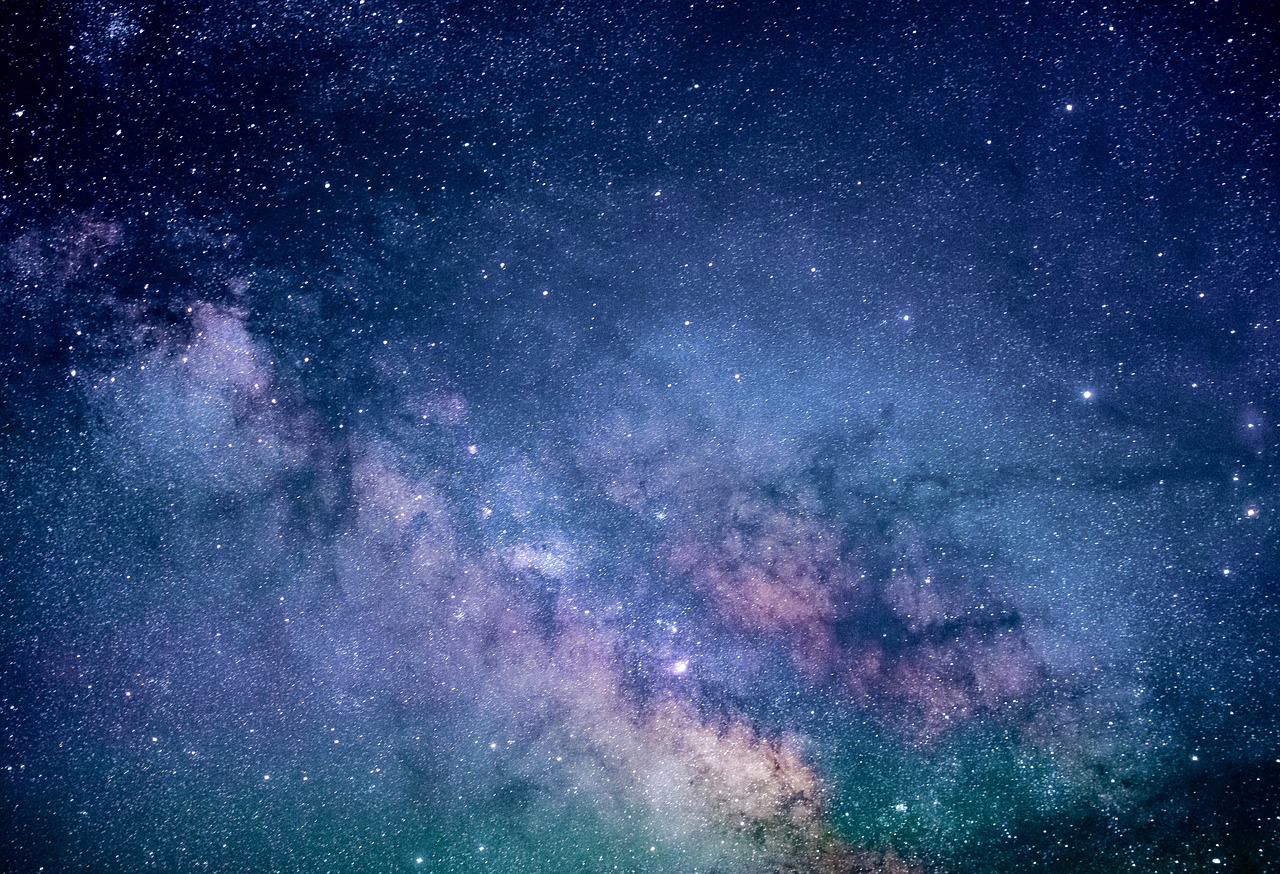
\includegraphics{Pictures/blue_space.jpg}}} % Image background
\$centering
\vspace*{11.3cm}
\par\normalfont\fontsize{35}{35}\sffamily\selectfont

\newpage
\begin{center}
    % List of Latex Colour names here: https://www.overleaf.com/learn/latex/Using_colours_in_LaTeX
    \textbf{\textsc{\color{Blue} \mytitle}}   % Modify the name of the colour used to suit your image
    
  %  \textbf{\color{White}(\ILMCode)} % Modify the name of the colour used to suit your image
    
   \color{black}\par % Modify the name of the colour used to suit your image
    
    \vspace*{4 cm}
    %\color{Apricot}\author % Modify the name of the colour used to suit your image
\begin{Huge}
 \textcolor{black}{Victoria Vampa}\\
\end{Huge}
    %(\id)\par  
\end{center}

\endgroup

%----------------------------------------------------------------------------------------
%	PARA TITULO USAR VERSALITA NEGRITA CENTRADO
%----------------------------------------------------------------------------------------
%\textsc{versalita}
%------------------------------------------------------------------



\chapter*{Agradecimientos}
Estoy muy agradecida a la Facultad de Ciencias Astronómicas y Geofísicas, por avalar la redacción de este texto,  y en especial al Dr. Adrián Brunini por haberme invitado en el año 2012 a elaborar una propuesta para que la asignatura Álgebra Lineal se dicte en la facultad.


Agradezco también a la Dra. Ana María Platzeck, por haberme brindado sus   notas de clase sobre tensores, ya que constituyeron  un aporte importante. 


Agradezco   especialmente  a lxs estudiantes, por las   valiosas contribuciones que han realizado a mis cursos   con sus comentarios y preguntas.
% \pagenumbering{Roman} % para comenzar la numeracion de paginas en numeros romanos
%\begin{flushright}
%\textit{Dedicado a los muchos alumnos,\\
%que a lo largo de un década\\
%me han ayudado a ser mejor docente.}
%\end{flushright}
\chapterimage{Pictures/blue_space(1).jpg} % Table of contents 
\chapter*{Prólogo}

Este libro es un texto de Álgebra Lineal destinado a estudiantes de la Licenciatura en Astronomía.
Es el resultado de enseñar durante muchos años los temas de Álgebra Lineal tanto en la Facultad de Ingeniería como en la Facultad de Ciencias Astronómicas y Geofísicas y de las contribuciones importantes que han realizado lxs  estudiantes, que han servido notablemente  al mejoramiento de mis clases.

He intentado lograr un equilibrio entre los desarrollos teóricos y las técnicas, escribiéndolos en forma detallada y dando ejemplos que ilustran su utilización. Para lograr una mejor comprensión de los conceptos teóricos, he puesto énfasis en la importancia de la interpretación geométrica. 


Quiero resaltar que la propuesta original sobre el curso ha sido  enriquecida con la contribución de la Licenciada en Astronomía Lucía Rizzo Buschiazzo,   quien incorporó  por un lado, problemas de aplicación diseñados especialmente para estudiantes de Astronomía y, por otro, una metodología novedosa promoviendo  la exposición oral de los trabajos prácticos.  

Creemos que este material elaborado resulta apropiado como apoyo y guía de estudio  para el desarrollo de la asignatura Álgebra Lineal que deben cursar lxs estudiantes de la carrera Licenciatura en Astronomía  en segundo año. Consideramos  que hemos podido  conectar los conceptos teóricos del Álgebra Lineal con  aplicaciones orientadas especialmente a esa disciplina. 

















%\newglossaryentry{latex}
%{
%    name=latex,
 %   description={Is a markup language specially suited for 
%scientific documents}
%}


%\newglossaryentry{formula}
%{
%    name=formula,
 %   description={A mathematical expression}
%}

%\end{document}

%The \Gls{latex} typesetting markup language is specially suitable 
%for documents that include \gls{maths}. \Glspl{formula} are rendered 
%properly an easily once one gets used to the commands.

\clearpage

%\printglossary

%\end{document}




%----------------------------------------------------------------------------------------
%	TABLE OF CONTENTS
%----------------------------------------------------------------------------------------
\renewcommand{\contentsname}{Índice}
\tableofcontents
\chapterimage{Pictures/blue_space(1).jpg} % Table of contents heading image
\vspace{12cm}
%\pagestyle{empty} % No headers
% \newpage
%\thispagestyle{empty} % para que no se numere esta pagina
 %% En esta secci'on se describe la estructura del documento de la tesis.
%% Consulta los reglamentos de tu universidad para determinar el orden
%% y la cantidad de secciones que debes de incluir.

%% # Portada de la tesis #
%% Mirar el archivo "titlepage.tex" para los detalles.

%% # Prefacios #
%% Por cada prefacio (p.e. agradecimientos, resumen, etc.) crear
%% un nuevo archivo e incluirlo aqu'i.
%% Para m'as detalles y un ejemplo mirar el archivo "gracias.tex"
\chapter*{Introducción}
\addcontentsline{toc}{chapter}{Introducción}
%\pagenumbering{Roman} % para comenzar la numeracion de paginas en numeros romanos
\vspace{1cm}
\section*{Introducción}

 \vspace{0.35cm}


El Álgebra Lineal es  una rama de la Matemática en la que se introducen numerosos conceptos abstractos. Es una disciplina de gran utilidad en la actualidad, en la resolución de problemas complejos y de grandes dimensiones. 
%Es una rama de la Matemática en la que se introducen numerosos conceptos abstractos, entre ellos, por ejemplo, los espacios vectoriales y las %transformaciones lineales. 

Este libro abarca los temas básicos de Álgebra Lineal   como son: espacios vectoriales, transforma-\ ciones lineales, diagonalización de una matriz y espacios vectoriales con producto interno. Si bien los temas tratados  son los mismos que aparecen en la mayoría de los textos introductorios al Álgebra Lineal, el punto de vista con que se enfoca la teoría y la ejercitación, se aparta del enfoque tradicional, y se enfatizan las aplicaciones. 
En todos los temas se establece la conexión fundamental con la interpretación geométrica. Se presenta una gran variedad de ejemplos y se proponen, además de ejercicios, actividades de investigación especialmente diseñadas para estudiantes de Astronomía. El texto tiene además un capítulo de cálculo tensorial y otro capítulo que describe  aplicaciones en la resolución de sistemas  ecuaciones diferenciales y en la aproximación de  funciones.  




En cuanto al origen, la palabra \textit{Álgebra}  procede del título de un  tratado  de un matemático, geógrafo y astrónomo persa conocido como Al-Juarismi. Vivió aproximadamente entre los años  780 y  850, en un tiempo de esplendor del mundo islámico. Su tratado,  el Hisab al-yabr wa’l muqabala  es un Compendio de cálculo por restauración y reducción \cite{lavanguardia}:
\begin{parchment}[Al-yabr]
%\lipsum[Al-yabr, restauración, la palabra del título que ha dado origen al término álgebra, es una de las operaciones básicas que ofrece %para resolver ecuaciones y que consiste en pasar los términos negativos de un lado de la ecuación como positivos al otro. Mientras que la %otra operación, la muqabala, consiste en simplificar la ecuación agrupando los términos similares.]
{Al-yabr, restauración, la palabra del título que ha dado origen al término álgebra, es una de las operaciones básicas que ofrece para resolver ecuaciones y que consiste en pasar los términos negativos de un lado de la ecuación como positivos al otro. Mientras que la otra operación, la muqabala, consiste en simplificar la ecuación agrupando los términos similares.}
%(Del artículo https://www.lavanguardia.com/cultura/20210520/7467794/bagdad-matematico-persa-fibonacci-algoritmo-algebra-cero-%guarismo.html).]
\end{parchment}
La historia del Álgebra Lineal moderna se remonta a mediados del siglo XIX con los trabajos de William Hamilton, quien introdujo el uso del término vector. Sin embargo, fue recién en la segunda mitad del siglo XX, cuando se incorporó al Álgebra Lineal   como una materia básica e introductoria en las matemáticas universitarias. 

Por sus múltiples aplicaciones, el estudio del Álgebra Lineal cobra cada día más importancia.  Su teoría es extensamente usada en el análisis funcional, en el análisis vectorial y en las ecuaciones diferenciales, entre otras áreas. Cabe señalar que sus numerosas aplicaciones no se restringen al campo de las ciencias exactas, sino que se extienden también al campo de las ciencias naturales y de las ciencias sociales.

%Es un texto interesante y peculiar.
%Al final del texto se incluten soluciones completas de las autoevaluaciones.
%Se usan notas al margen para ayudar al lector no solo a identificar los conceptos sino para   resaltar algunas propiedades de interés.


%En este curso semestral les proponemos no sólo que incorpore los nuevos conceptos sino que también ejercite su capacidad de investigación y la de %trasmitir sus hallazgos, lo cual es igual de importante.

Con la escritura de este libro he intentado  hacer interesantes y accesibles los temas de Álgebra Lineal, equilibrando los desarrollos teóricos con las técnicas que se utilizan en las aplicaciones, pretendiendo proporcionar a lxs estudiantes las habilidades algebraicas necesarias para resolver problemas. He resaltado las interpretaciones geométricas de conceptos importantes, como las transformaciones lineales y el producto interno. 

El texto tiene siete capítulos, con una breve introducción al comienzo de cada uno de ellos.  Para facilitar la lectura, en todos los capítulos se ha  indicado con \tikz{\fill[orange!25] (0,0) circle (0.3cm);
\node at (0,0) {\textcolor{blue}{\fontfamily{qcr}\selectfont{i}}};} a las  observaciones importantes. Además, para una mejor comprensión de los temas, se han incluído numerosos ejemplos. 


%\textcolor{blue}{{\fontfamily{qcr}\selectfont{i}}} 
En cada capítulo, las actividades propuestas contemplan  un problema de aplicación que el estudiante debe realizar y presentar y luego una serie de ejercicios  prácticos y teóricos. Al final, se presenta una autoevaluación  que le servirá al estudiante  para saber qué temas debe reforzar y cuyas respuestas se presentan al final del libro.


En cuanto a los conocimientos previos que se requieren, en el Apéndice se presentan  una serie de ejercicios  como 'precalentamiento' que facilitarán al estudiante el abordaje del libro. 

Por último y para estimular al lector el interés sobre el desarrollo histórico de los temas, se incluyen varias notas históricas dispersas  a lo largo del libro, y   semblanzas breves sobre científicos  que han realizado aportes muy valiosos al desarrollo del Álgebra Lineal. 

Sobre el template 
% The original template (the Legrand Orange Book Template) can be found here --> %http://www.latextemplates.com/template/the-legrand-orange-book
%
% Original author of the Legrand Orange Book Template::
% Mathias Legrand (legrand.mathias@gmail.com) with modifications by:
% Vel (vel@latextemplates.com)

Sobre la imagen de portada

%Imagen en la portada de los capítulos: Nebulosa Roseta, IC 1396B, obtenida por el relevamiento fotométrico IPHAS/N, preparada por  Nick Wright.
%\newpage

% \begin{flushleft}

% \end{flushleft}
%\begin{figure}[h] %Puts the image here
  %  \centering
   % 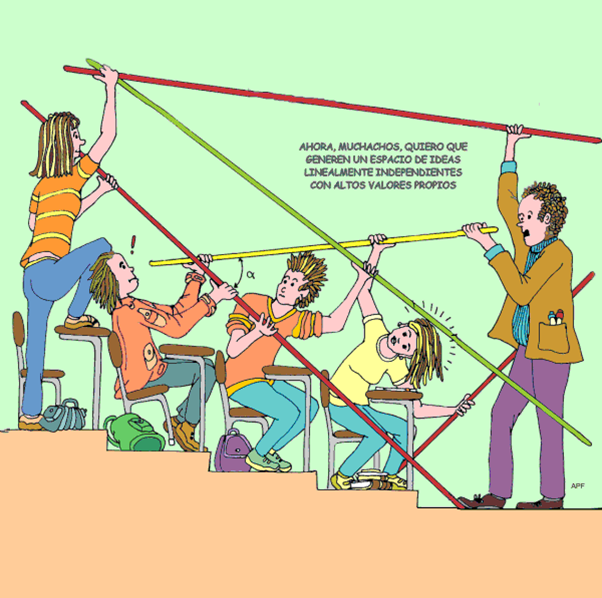
\includegraphics[width=0.7\textwidth]{Pictures/lineal.png} % If you want a smaller image you can change the width to [width=0.5\textwidth] or any percentage. This scales automatically, so will not become squashed or stretched 
%\end{figure}

%\listoftables %uncomment this if you want to print the list of tables at the start

%\pagestyle{fancy} % Print headers again


%----------------------------------------------------------------------------------------
%	Glossary
%----------------------------------------------------------------------------------------
%\newpage
%\chapterimage{Pictures/blue_space(1).jpg} % Table of contents heading image
%\printglossary


%\printglossaries

%----------------------------------------------------------------------------------------
%	First set of related questions
%----------------------------------------------------------------------------------------

\


%--------------------------------------------------------------}Second set of related questions
%----------------------------------------------------------------------------

\chapterimage{Pictures/blue_space(1).jpg}
%\chapter{Espacios Vectoriales}
%El concepto de espacio vectorial generaliza las propiedades que tienen las operaciones de suma y producto por escalares  para los vectores de %$\mathbb{R}^2$ y $\mathbb{R}^3$. Abordaremos en este capítulo la estructura de espacio vectorial, objeto básico de estudio del Álgebra Lineal. A sus %elementos se los denomina vectores, independientemente de su naturaleza.

\chapter{Espacios Vectoriales}

El concepto de espacio vectorial generaliza las propiedades que tienen las operaciones de suma y producto por escalares  para los vectores de $\mathbb{R}^2$ y $\mathbb{R}^3$. Abordaremos en este capítulo la estructura de espacio vectorial, objeto básico de estudio del Álgebra Lineal. A sus elementos se los denomina vectores, independientemente de su naturaleza.

\bigskip


\section{Definición de espacio vectorial. Ejemplos  }\label{intro}


El conjunto de los números reales y el conjunto de los números complejos, con los cuales ya se trabajó, tienen propiedades similares. En ambos conjuntos pueden definirse dos operaciones $+$ y $.$ que satisfacen ciertas propiedades y reciben el nombre de  \textit{cuerpo}. Trabajaremos tanto con el cuerpo de los reales,  $\mathbb{R}$ como con el cuerpo de los complejos  $\mathbb{C}$, denotándolos por K.
Al estudiar vectores en el plano y en el espacio, se ha definido la \textit{suma de vectores} y la \textit{multiplicación por un número real}, y se vieron las propiedades que satisfacían. También para el conjunto de polinomios. 
Cuando en varios conjuntos distintos aparecen estructuras similares es conveniente axiomatizar éstas y darles un nombre al ente resultante, con la ventaja que estudiando esta estructura, quedan estudiadas todas las estructuras que en ella se encuadran. Cuando en un conjunto se da una estructura similar a la de los ejemplos anteriores, se dice que se tiene un \textit{espacio vectorial}.

\bigskip

\bigskip
 

\bigskip


\begin{definition}\index{Espacio Vectorial}
    {Un conjunto $V$, cuyos elementos se denotan mediante $\vec{u}$, $\vec{v}$, $\vec{w}$, se dice que es un \textit{espacio vectorial} sobre el cuerpo $K$, si en él se han definido dos operaciones: la \textit{suma}, de manera que a cada par de elementos $\vec{u}$ y $\vec{v}$ de $V$ se le hace corresponder el elemento $\vec{u}+\vec{v}$ de $V$, denominado suma de $\vec{u}$ y $\vec{v}$, y la \textit{multiplicación por escalares}, de manera que a todo elemento $\vec{u}$ de $V$  y a todo elemento $a$ de $K$ se le hace corresponder el elemento $a\vec{u}$ de $V$, y se satisfacen las siguientes propiedades:

\bigskip

%\vskip0.5cm

\begin{enumerate}
%\item[]\textbf{EJEMPLO 1:}


\item Conmutativa $~\vec{u}~ + ~\vec{v}~ = ~\vec{v}~ + ~\vec{u}~$ $~~\forall$ $\vec{u}$ y $\vec{v}$ $\in$ $V$.

\item Asociativa $~\vec{u}~ + (~\vec{v}~+  ~\vec{w}~)= (~\vec{u}~+  ~\vec{v}~) + ~\vec{w}~$,$~~\forall$ $\vec{u}$,  $\vec{v}$ y $\vec{w}$  $\in$ $V$. 
\item Existe un elemento de $V$, designado por $\vec{0}$ y denominado \textit{elemento neutro}, tal que 
$~\vec{u}~ + ~\vec{0}~ = ~\vec{u}~$ $\forall$ $\vec{u}$ $\in$ $V$.

\item Para todo elemento $\vec{u}$ $\in$ $V$, existe un elemento designado por $-\vec{u}$ y denominado \textit{elemento opuesto} de $\vec{u}$, tal que 
$~\vec{u}~ + ~(-\vec{u})~ = ~\vec{0}$

\item $1~\vec{u}~ =~\vec{u}~$ $\forall$ $\vec{u}$ $\in$ $V$, donde $1$ denota el elemento unidad del cuerpo  $K$. 

\item $a(b~\vec{u}~) =(ab)~\vec{u}~$ $~~\forall$ $\vec{u}$ $\in$ $V$, y $~~\forall$ $a$ y $b$ $  \in K$.
\item $(a+b)~\vec{u}~ =a~\vec{u}~+b~\vec{u}~ $ $\forall$ $\vec{u}$ $\in$ $V$, y todo $a$ y $b$ $\in$ K.
\item $a(~\vec{u}~+~\vec{v}~) =a~\vec{u}~+a~\vec{v}~ $ $\forall$ $\vec{u}$, $\vec{v}$ $\in$ $V$, y $\forall$ $a$ $\in$ K.

\end{enumerate}}
\end{definition}

\bigskip

\bigskip

En la Figura  \ref{fig:my_label} se muestra la propiedad conmutativa $1$.

%\begin{tikzpicture}[scale=1.5]
    % Draw axes
    %\draw [<->,thick] (0,2) node (yaxis) [above] {$y$}
        %|- (3,0) node (xaxis) [right] {$x$};
    % Draw two intersecting lines
    %\draw (0,0) coordinate (a_1) -- (2,1.8) coordinate (a_2);
    %\draw (0,1.5) coordinate (b_1) -- (2.5,0) coordinate (b_2);
    % Calculate the intersection of the lines a_1 -- a_2 and b_1 -- b_2
    % and store the coordinate in c.
    %\coordinate (c) at (intersection of a_1--a_2 and b_1--b_2);
    % Draw lines indicating intersection with y and x axis. Here we use
    % the perpendicular coordinate system
    %\draw[dashed] (yaxis |- c) node[left] {$y'$}
       % -| (xaxis -| c) node[below] {$x'$};
    % Draw a dot to indicate intersection point
    %\fill[red] (c) circle (2pt);
%\end{tikzpicture}

%\begin{tikzpicture} % ejes
%\draw[thin, blue] (0,0) -- (0,2) node (yaxis) [above] {$z$};
%\draw[thin, blue] (0,0) -- (2,0)  node (xaxis) [above] {$y$};
% segmento
%\draw[thin, blue]
%(0,0) -- (-1,-1) node (zaxis) [above] {$x$};
%\end{tikzpicture}


%\vskip0.5cm
%\tikzset{ % Lista de opciones de nodo
% opción draw = color borde
% opacity = porcentaje transparencia
% opción fill = color relleno
%opciones/.style={%
%draw= red!50!black!50,
%top color = white,
%bottom color = red!50!black!20,
%fill opacity = 0.6,
%rectangle, font=\small\bf\sffamily}
%}
%\begin{center}
%\begin{tikzpicture}
%\draw[draw= yellow!30,fill=yellow!30] (0,0) rectangle(2,2);
%\node[draw=black,rectangle, anchor=center] at (1,1) {$\bullet$};
%\node[opciones, anchor=south east] at (1,1) {ancla en el sur-este};
%\node[opciones, anchor=north west] at (1,1) {ancla en el norte-oeste};
%\end{tikzpicture}
%\caption{figure}{Nodos rectangular con anclaje en el sureste y noroeste}
%\end{center}
%\begin{tikzpicture}
%\draw[thick,->] (0,0,0) -- (1,0,0) %node[anchor=north east]{$x$};
%\draw[thick,->] (0,0,0) -- (0,1,0) node[anchor=north west]{$y$};
%\draw[thick,->] (0,0,0) -- (0,0,1) node[anchor=south]{$z$};
%\end{tikzpicture}

\begin{figure}
    \centering
    %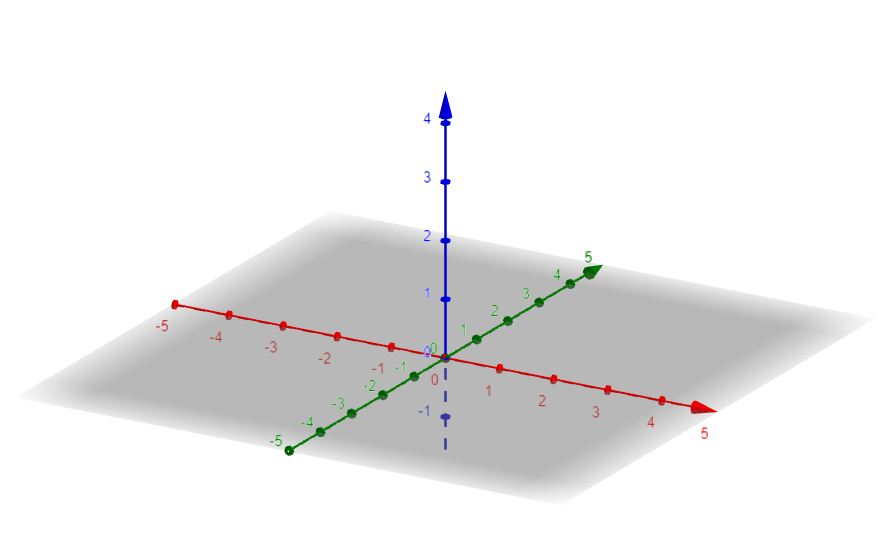
\includegraphics[width=0.60\textwidth]{Pictures/geogebra-export.png}
    %\caption{Caption}
    \label{fig:my_label}
\end{figure}
\begin{figure}
    \centering
    %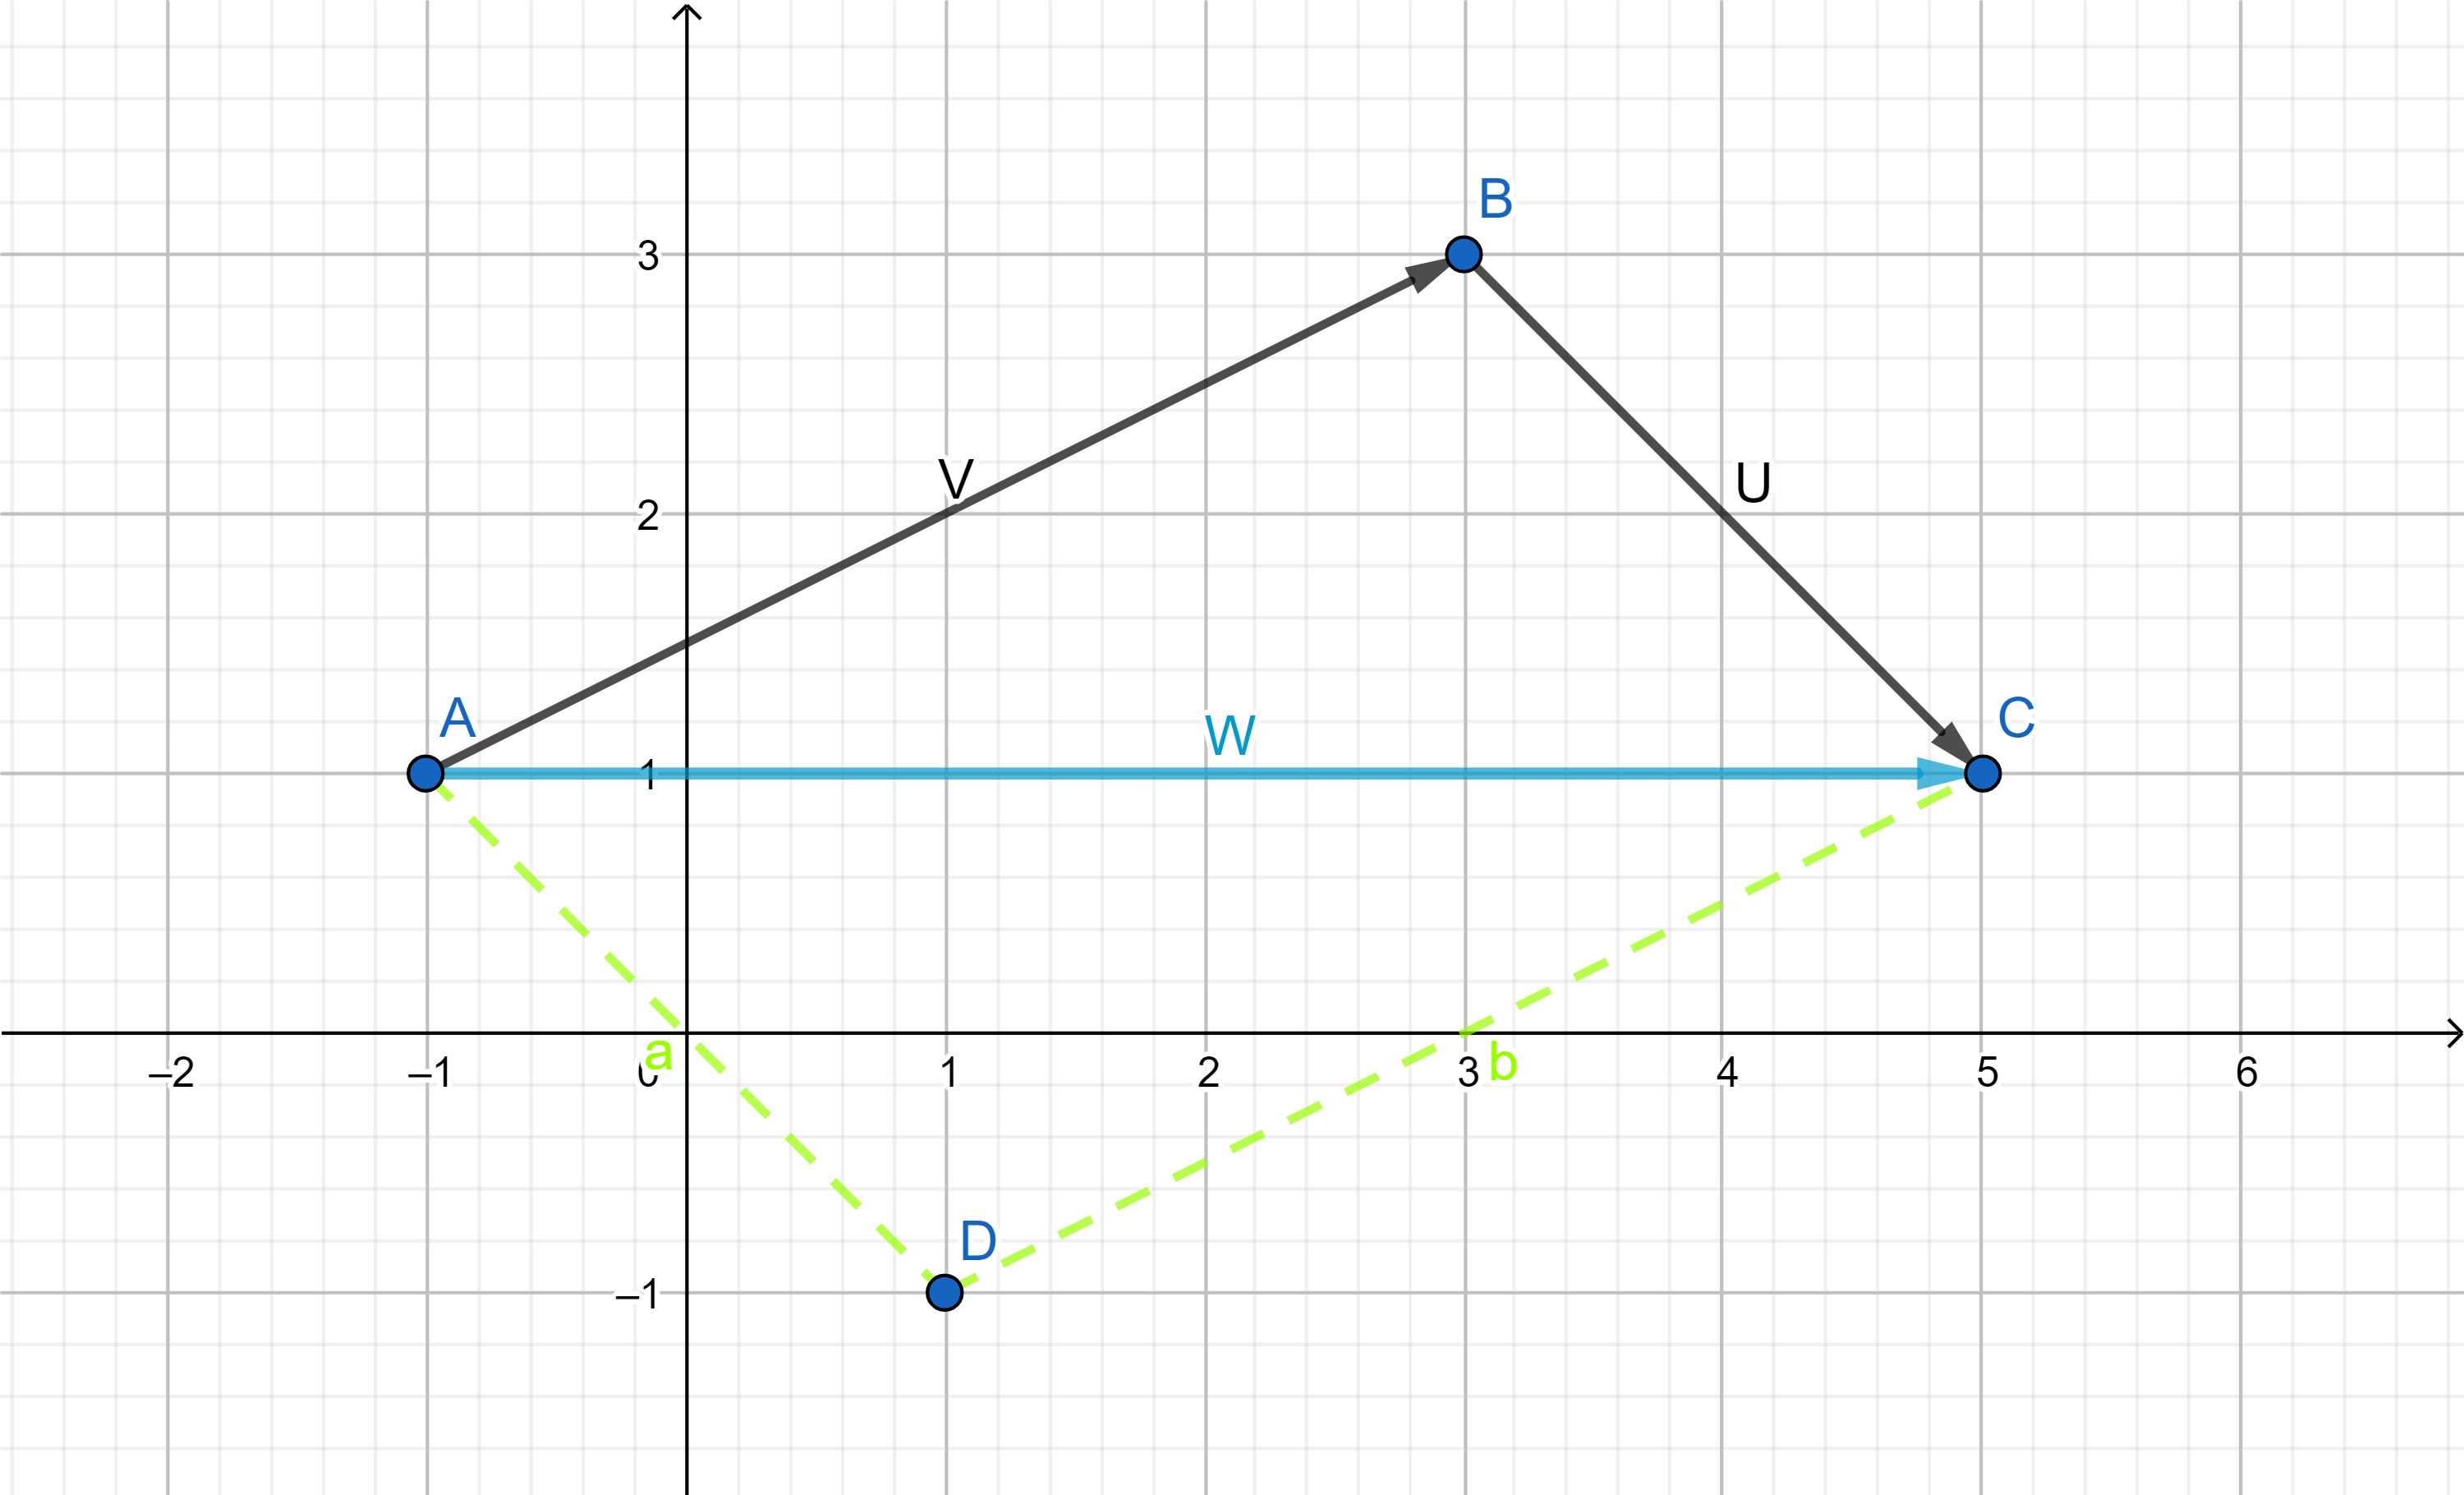
\includegraphics[width=0.60\textwidth]{Pictures/suma de vectores.png}   
\end{figure}



\begin{figure}
    \centering
    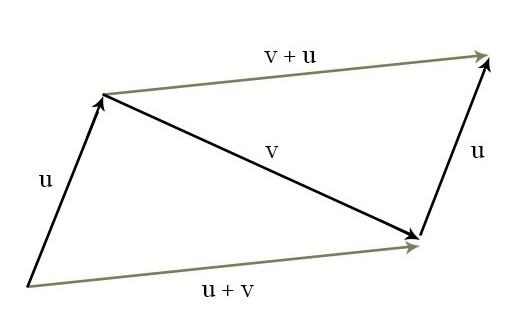
\includegraphics[width=0.50\textwidth]{Pictures/fig.40d.jpg}
   \caption{$~\vec{u}~ + ~\vec{v}~ = ~\vec{v}~ + ~\vec{u}~$}
    \label{fig:suma}
\end{figure}

\bigskip


\bigskip

\bigskip

\begin{remark} 
%$\\$
%\vspace{1.5cm}
\begin{itemize}

\item 

Los elementos del espacio vectorial reciben el nombre genérico de \textit{vectores}.
\item 
Las primeras cuatro propiedades se refieren a la suma en $V$, las dos que siguen a la multiplicación de elementos de $V$  por escalares y las dos últimas son las propiedades distributivas de una operación con respecto a la otra.
\item 
Si K es $\mathbb{R}$ se dice que $V$ es \textit{un espacio vectorial real}, y si K es  $\mathbb{C}$ se dice que es \textit{un espacio vectorial complejo}.
\end{itemize}
%\hfill$\blacktriangle$
\end{remark}

%\begin{enumerate}[label=\itembolasazules{\arabic*}]

\begin{example}
$\mathbb{R}$ es un espacio vectorial sobre $\mathbb{Q}$, $\mathbb{C}$ es un espacio vectorial sobre $\mathbb{R}$ y  sobre $\mathbb{Q}$.
$\mathbb{R}^{2}$ o $\mathbb{R}^{3}$ (vectores en el plano, o en el espacio), con las operaciones usuales son espacios vectoriales sobre $\mathbb{R}$.
\end{example}

\bigskip

\begin{example}   
$$K^n=\{(x_1,x_2, \cdots, x_n), ~ x_j \in K, j=1,2, \cdots, n\}$$
con las operaciones usuales es un espacio vectorial sobre K. En particular, $\mathbb{R}^{n}$ es un espacio vectorial real y  $\mathbb{C}^{n}$ es un espacio vectorial complejo.
\end{example}

\bigskip

\begin{example}
Sea $P_K \left[x\right]$ el conjunto de todos los polinomios en la variable $x$ sobre el cuerpo $K$, es decir, todos los elementos de la forma
$$p(x)= a_0 + a_1 x +a_2 x^2 + \cdots + a_n x^n  + \cdots $$ 
donde los coeficientes $a_j \in K$ con las operaciones suma de polinomios y multiplicación por escalares.  $P_K\left[x\right]$ es un espacio vectorial sobre $K$.
\end{example}

\bigskip


\begin{example} 
Sea $C(\left[a,b\right])$ el conjunto de todas las funciones continuas definidas en el intervalo real $[a,b]$, con valores en $\mathbb{R}$, $\left \{ f: [a,b]  \rightarrow  \mathbb{R} \right \}$ con las operaciones suma de funciones,

$$(f+g)(x)=f(x)+g(x),$$ y multiplicación de una función por un escalar,
$$(af)(x)=a(f(x)).$$
Puede comprobarse fácilmente  que  $C([a,b])$ es un espacio vectorial. El elemento neutro es la función nula.
\end{example}


\bigskip


\begin{example} 
El conjunto $S(A)$ de soluciones del sistema homogéneo $A\vec{X}=\vec{0}$, donde $A \in \mathbb{R}^{m \times n}$ y $\vec{X}=(x_1, x_2, \cdots, x_n)$ $\in \mathbb{R}^{n}$ es un  espacio vectorial sobre $\mathbb{R}$. Es un subespacio de  $\mathbb{R}^{n}$.
\end{example}

\bigskip

\begin{remark}
Los siguientes son algunos resultados que se deducen de las propiedades que definen un espacio vectorial y se dejan como ejercicio para el lector.

\begin{itemize}
\item[$\bullet$]  El elemento neutro de un espacio vectorial es único. 

\item[$\bullet$]  El opuesto de cada elemento en un espacio vectorial es único. 

\item[$\bullet$]   Para todo $\vec{u}$ de un espacio vectorial $V$, $0.\vec{u}=\vec{0}$. 


\item[$\bullet$] Para todo elemento $\vec{u}$ de un espacio vectorial $V$, $(-1)\vec{u}$ es su opuesto.

\item[$\bullet$] En todo espacio vectorial $V$, $a$ $\vec{0}=\vec{0}$, donde $a\in $K y $\vec{0}$ es el elemento neutro de $V$.

\end{itemize}
\end{remark}


\section{Subespacio vectorial}
\label{Subespacio vectorial}
Algunos subconjuntos de un espacio vectorial $V$ son a su vez espacios vectoriales con las operaciones definidas en $V$; estos subconjuntos especiales reciben el nombre de \textit{subespacios vectoriales} de $V$.

\bigskip

\begin{definition}\index{Subespacio vectorial}
Un \textit{subespacio vectorial} de un espacio vectorial $V$ es un subconjunto $S$ no vacío  de $V$, que a su vez es un espacio vectorial con las operaciones definidas en $V$.
\end{definition}


\bigskip

\begin{remark}
Para demostrar que un subconjunto  $S$ es un subespacio vectorial no es necesario comprobar de nuevo que satisface todas las propiedades del espacio vectorial. Es suficiente demostrar que  contiene al vector nulo, que la suma de dos elementos de $S$ es otro elemento de $S$, y que la multiplicación de un elemento de $S$ por un elemento del cuerpo K, es otro elemento de $S$:


\bigskip

 
\begin{enumerate}
\item  $\vec{0} \in S$
\item Si $\vec{u}$ y $\vec{v}$ $ \in$ $S$, $~\vec{u}~+  ~\vec{v}~$ $ \in$ $S$

\item Si $a$ $ \in$ $K$ y $\vec{u}$ $ \in$ $S$, $a~\vec{u}~$ $\in$ $S$

\end{enumerate}
%\hfill$\blacktriangle$
\end{remark}


\begin{figure}
    \centering
    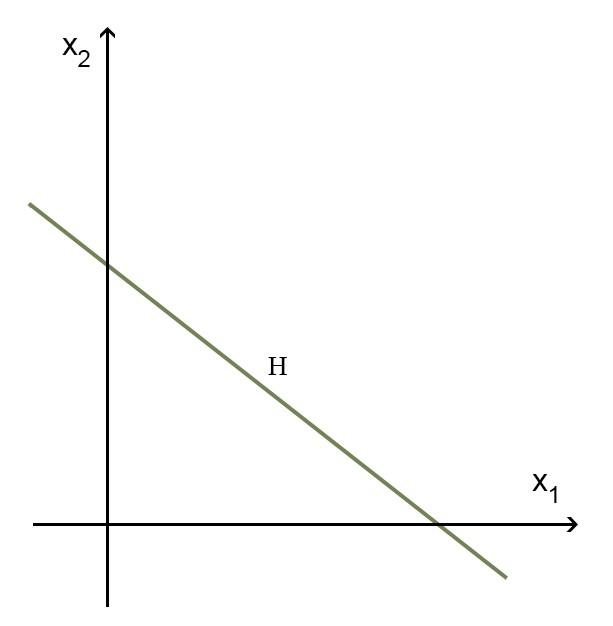
\includegraphics[width=0.40\textwidth]{Pictures/fig.41.jpg}
   \caption{Recta que no pasa por el origen. }
    \label{rectanon}
\end{figure}
%\begin{center}
 %\begin{tikzpicture}[scale=1.5]
 %\label{rectano}
    % Draw axes
    %\draw [<->,thick] (0,2) node (yaxis) [above] {$x_2$}
      %  |- (3,0) node (xaxis) [right] {$x_1$};
       %     \draw[line width =0.051cm, blue]  (-0.5,1.5) -- (2.5,-0.5);
    %\draw [thick] (1.2,1) node[below]{$H$};
 %\end{tikzpicture}
%\caption{ Figura 2.2. Una recta que no pasa por el origen no es un subespacio vectorial  de $\mathbb{R}^2$.}
%\caption{Una recta que no pasa por el origen no es un subespacio vectorial  de $\mathbb{R}^2$.}
%\end{center}
%\begin{figure}
 %   \centering
    %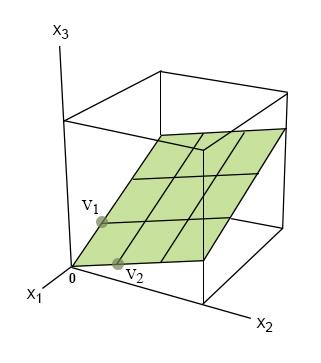
\includegraphics[width=0.50\textwidth]{Pictures/EVfig.2.jpg}
   
    %\label{EVfig. 2}
%\end{figure}
%\begin{example}
%{$S=\{(0,0)\}$ es un subespacio}

%\bigskip


\begin{example}
Sea $V$ un espacio vectorial sobre $K$. $S=\{\vec{0}\}$ es un subespacio de $V$.
\end{example}
\begin{example}
$V$ es un subespacio de $V$.
\end{example}




\begin{example}
Veamos cómo  caracterizar los subespacios de $\mathbb{R}^2$.
\begin{enumerate}
\item
$S=\{(0,0)\}$ es un subespacio.

\item 
Supongamos $S$ un subespacio que contiene algún elemento $\vec{u}$ no nulo. Entonces para todo $a$ $\in R$, $a\vec{u}$ $\in S$. Si esos son todos los elementos de $S$, $S$ es un subespacio y gráficamente es una recta por el origen.

\item 

Si $S$ contiene a un $ \vec{v}$ que no es $a \vec{v}$, contiene a sus múltiplos $a \vec{v}$. 
Luego contiene a dos rectas $L_{\vec{u}}$ y $L_{\vec{v}}$ por el origen. Por la regla del paralelogramo cualquier $\vec{w}$ $\in$ $\mathbb{R}^2$ es suma de un elemento de $L_{\vec{u}}$ y uno de $L_{\vec{v}}$. En consecuencia $S=\mathbb{R}^2$.
\end{enumerate}

\bigskip

Los subespacios de $\mathbb{R}^2$ son entonces, el vector nulo, las rectas por el origen y todo $\mathbb{R}^2$.
\end{example}

\bigskip

\begin{example}
\label{rectanonueva}
Sea $H=\{(x,y) \text{ tales que } y=mx+b \quad m, b \in \mathbb{R}, ~ b \neq 0 \}$ 
(Ver Figura \ref{rectanon}).
$H$ no es un subespacio de $\mathbb{R}^2$. Ya que si $(x_1,y_1)$ y $(x_2,y_2)$  son $2$ puntos sobre la recta $y=mx+b$, $y_1=m x_1+ b$ e $y_2=m x_2+ b$, se tiene que  $y_1+y_2= m(x_1+x_2) + 2 b$,  y entonces, $y_1+y_2  \notin H$.
O bien, directamente,  no es subespacio de $\mathbb{R}^2$ porque $(0,0) \notin H$.
\end{example}
\begin{figure}
    \centering
    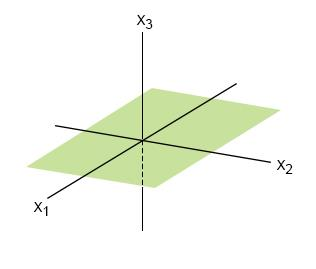
\includegraphics[width=0.60\textwidth]{Pictures/EVfig.1.jpg}
    \caption{El plano $x_1x_2$ es un subespacio de $\mathbb{R}^3$ }
    \label{EVfig.1}
\end{figure}
%\begin{example}
%El  plano por el origen $x_3=0$  (Figura \ref{EVfig.1}) es un subespacio de $\mathbb{R}^3$
%\end{example}
%\vskip1.5cm
\begin{example}
Si $\vec{v}$  $ \in$ $V$, $S=\{a\vec{v}, a\in K \}$ es un subespacio de $V$. Este subespacio se denomina el subespacio generado por $\vec{v}$, y se nota $S=\left\langle \vec{v}\right\rangle$.
\label{ejgenv}
\end{example}

\bigskip
\begin{theorem}
\label{PROP121}
%\begin{thm}
Sean $\vec{v}_1,\vec{v}_2,\cdots,\vec{v}_n$ $ \in$ $V$. Entonces $S=\{a_1 \vec{v}_1+a_2 \vec{v}_2+\cdots +a_n\vec{v}_n, ~ a_i ~ \in K \}$ es un subespacio de $V$. 
\noindent
\begin{proof}

\begin{itemize}
\item
$\vec{0}\in S$ ya que 
$\vec{0} =0 \vec{v}_1+0 \vec{v}_2+\cdots +0\vec{v}_n, ~ 0 ~ \in K $.

\item
Si
 $\vec{u} =a_1 \vec{v}_1+a_2 \vec{v}_2+\cdots +a_n\vec{v}_n, ~ a_i ~ \in K$ y
 
 $\vec{w} =b_1 \vec{v}_1+b_2 \vec{v}_2+\cdots +b_n\vec{v}_n, ~ a_i ~ \in K $,
 entonces
 
 $\vec{u}+\vec{w} =(a_1+b_1) \vec{v}_1+(a_2+b_2) \vec{v}_2+\cdots +(a_n+b_n)\vec{v}_n, 
 
 con (a_i+b_i) ~ \in K $, por lo tanto, $  \vec{u}+\vec{w} \in S$.
 \item
 Si $\alpha \in K$
 $ \alpha \vec{u} = (\alpha a_1) \vec{v}_1+  (\alpha a_2) \vec{v}_2+\cdots + (\alpha a_n)\vec{v}_n, ~ (\alpha a_i) ~ \in K $, por lo tanto $  \alpha \vec{u}  \in S$
 \end{itemize}
 Se tiene, entonces, que $S$ es un subespacio de $V$.
 \end{proof}
%\end{thm}
\end{theorem}





\begin{remark}
El espacio vectorial $\mathbb{R}^2$ no es un subespacio de $\mathbb{R}^3$. $\mathbb{R}^2$ ni siquiera es un subconjunto  de $\mathbb{R}^3$.  En cambio el conjunto


$$S=\left \{ \left( \begin{array}{c} x_1 \\ x_2 \\ 0\end{array}\right) \quad x_1,~x_2 \in \mathbb{R}   \right\}$$

\bigskip
\noindent
sí es un subconjunto y un subespacio de $\mathbb{R}^3$ (Ver Figura \ref{EVfig.1}).
%\hfill$\blacktriangle$
\end{remark}


\begin{example}
 $P_\mathbb{R}^{(n)}\left[t\right]$ (polinomios en $t$  de grado $\leq n$, con coeficientes reales) es un subespacio vectorial de $P_\mathbb{R}\left[t\right]$; a su vez, $P_\mathbb{R}\left[t\right]$ es un subespacio vectorial  del espacio vectorial de las funciones continuas en $\mathbb{R}$.
\end{example}
% figuras subespacios

\begin{figure}
    \centering
    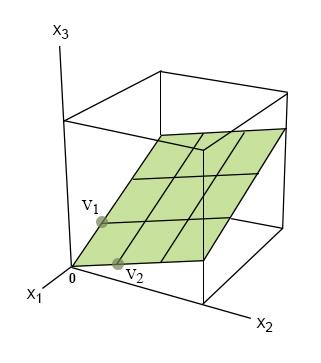
\includegraphics[width=0.50\textwidth]{Pictures/EVfig.2.jpg}
    \caption{Subespacio generado por $\vec{v}_1$ y $\vec{v}_2$ }
    \label{EVfig. 2}
\end{figure}


\begin{example}\index{Combinación lineal}
\label{ejemploLS}
Sea $S=\left\{\vec{u}_1,\vec{u}_2,\cdots,  \vec{u}_n\right\}$ un conjunto de $n$ vectores de un espacio vectorial $V$. Consideremos como en el Ejemplo \ref{ejgenv}  pero con más vectores.
Se define el conjunto de todas las combinaciones lineales de los vectores de $S$, 
$$\bold{L}(S)=\bold{L}(\vec{u}_1,\vec{u}_2,\cdots,  \vec{u}_n)=\left\{\sum_{j=1}^{n}a_j\vec{u}_j,  ~ ~a_j\in K, j=1,2,\cdots,n\right\}$$
El conjunto $\bold{L}(S)$ es un subespacio vectorial de $V$ (ver Proposición \ref{PROP121}), que recibe el nombre de \textsl{subespacio vectorial generado por $S$}. 

En $\mathbb{R}^3$, si $\vec{v}_1$ y $\vec{v}_2$ son dos vectores tales que uno no es múltiplo del otro, entonces,  $\bold{L}(\vec{v}_1,\vec{v}_2,  )$ es un plano que pasa por el origen.  Es un subespacio de $\mathbb{R}^3$; se muestra en la  Figura \ref{EVfig. 2}.




\end{example}

%\vskip1.5cm

\begin{example}
\label{ejintsub}
Sean $a_1, a_2, \cdots, a_n \in K $ fijos.  

$S=\{ (x_1,x_2,\cdots, x_n) \in K^n, a_1x_1+a_2x_2+\cdots +a_nx_n=0\}$ es un subespacio de $K^n$.
\end{example}
%figura Nul A


\begin{example}\index{Espacio nulo de una matriz}
\label{ejsistema}
Dada una matriz $A \in \mathbb{R}^{m \times n}$ , y de rango $r$, todas las soluciones del sistema de ecuaciones homogéneo
$$A\vec{X}=\vec{0}, \qquad  \vec{X}\in \mathbb{R}^n$$
constituyen un subespacio vectorial de $\mathbb{R}^n$, conocido como \textit{espacio nulo} de la matriz $A$. Se anota $Nul(A)$  y se muestra en la  Figura \ref{EVfig. 3.}.


\bigskip

Para el sistema homogéneo:
\begin{equation} 
\left\{ \begin{array} {ccl} \nonumber
                    2y-z+w &\ =&0      \\
                     3x+y+10z+5w &\ = &0  \\
                    x+3z + w &\ =&0 \label{ejemplosist}
                   \end{array}
           \right.
\end{equation}

\bigskip
\noindent
luego de realizar operaciones elementales sobre las filas de la matriz de coeficientes del sistema (método de eliminación gaussiana), se llega a la matriz escalonada:

\[ \left( \begin{array}{cccc}
3 & 1 & 10 & 5\\0 & 2 & -1 &1  \\ 0 & 0 & -1/2 & 1/2 
\end{array}
\right )
\]

\bigskip

\noindent
de donde la solución es $z=-w$, $y=-w$ y $x=2w$. El subespacio  de soluciones del sistema homogéneo es, entonces,

$$S=Nul(A) = \langle (2,-1,-1,1) \rangle $$
\end{example}
%\end{enumerate}


\begin{figure}
    \centering
    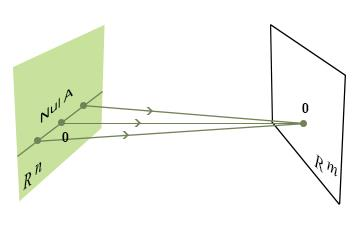
\includegraphics[width=0.60\textwidth]{Pictures/EVfig.3.jpg}
    \caption{Espacio nulo de una matriz $A$.}
    \label{EVfig. 3.}
\end{figure}

\begin{remark}
\label{SHSNH}
Así como vimos que las rectas que no pasan por el origen no son un subespacio de $\mathbb{R}^2$ (Ejemplo  \ref{rectanonueva}), las soluciones de un sistema no homogéneo 
$$A\vec{X}=\vec{b}, \qquad  \vec{b} \neq \vec{0}$$  son un subconjunto pero no un subespacio de    $\mathbb{R}^n$.
%\hfill$\blacktriangle$
\end{remark}

\bigskip

\index{Hamilton, William R.}
\begin{parchment}[William Rowan Hamilton (1805 - 1865)]{ Fue un matemático británico. Fue uno de los fundadores de la escuela británica moderna de matemáticas puras e hizo importantes contribuciones al desarrollo de la óptica, la dinámica, y el álgebra. Su descubrimiento del cuaternión, junto con su sistematización de la dinámica, son sus trabajos más conocidos. Este último trabajo sería decisivo en el desarrollo de la mecánica cuántica, donde un concepto fundamental llamado hamiltoniano lleva su nombre.
Hamilton fue el cuarto de los nueve hijos. Vivían en Dublín. Se dice que Hamilton demostró un inmenso talento a una edad muy temprana. 
Su tío observó que Hamilton, había mostrado una asombrosa habilidad para aprender idiomas. A la edad de siete años, ya había hecho un progreso considerable con el hebreo, y antes de los trece años, bajo la supervisión de su tío (un lingüista), había adquirido conocimientos casi en tantos idiomas como años de edad tenía (idiomas europeos clásicos y modernos, y persa, árabe, hindustaní, sánscrito e incluso maratí y malayo).
Hamilton es reconocido como uno de los científicos más destacados de Irlanda, y a medida que la nación se vuelve más consciente de su herencia científica, cada vez se lo celebra más. Se dice que se le permitía pisar el césped de la Universidad, algo totalmente prohibido. Este hecho camina entre la realidad y la ficción. Posiblemente ocurriera que, absorto en sus meditaciones, descuidara esta prohibición y accidentalmente caminase por los jardines. Esta anécdota seguramente sirve para dar idea de la categoría de Hamilton como uno de los grandes matemáticos de su tiempo y de la historia.
El Instituto Hamilton está dedicado a la investigación sobre matemáticas aplicadas en la Universidad Maynooth. 
Irlanda emitió dos sellos conmemorativos en 1943 para celebrar el centenario del anuncio de los cuaterniones. El Banco Central de Irlanda acuñó en 2005 una moneda de plata conmemorativa de 10 euros para conmemorar los 200 años desde su nacimiento.
Los talleres de mantenimiento más nuevos del sistema de tranvías de Dublín (LUAS), llevan su nombre.

En su juventud, Hamilton tuvo un telescopio y se convirtió en un experto en el cálculo de fenómenos celestes, como por ejemplo, la determinación de la visibilidad de los eclipses de luna. Fue elegido Astrónomo Real de Irlanda y se instaló en el Observatorio de Dunsink, donde permaneció hasta su muerte en 1865.
Hoy en día, Hamilton no es reconocido como un gran astrónomo, aunque durante su vida si gozó de esta consideración. Sus conferencias de introducción a la astronomía fueron famosas; además de sus alumnos, atrajeron a muchos eruditos y poetas, e incluso a damas; en aquellos días una hazaña notable. La poetisa Felicia Hemans escribió su poema "La oración del estudiante solitario" después de escuchar una de sus conferencias.  \cite{hamilton}}
\end{parchment}

\bigskip

\section{Base y dimensión de un espacio vectorial}\index{Independencia lineal}\index{Sistema de generadores}

Sea $V$ un espacio vectorial sobre un cuerpo K; un número finito de vectores  $\vec{v}_1, \vec{v}_2, ,\cdots, \vec{v}_n$  se dice que son \textit{linealmente dependientes} si existen $n$ elementos de K, $a_1, a_2, ,\cdots, a_n$  no todos nulos, tal que 
$$a_1\vec{v}_1+a_2\vec{v}_2+\cdots +a_n\vec{v}_n=\vec{0}$$

Si los vectores $\vec{v}_1, \vec{v}_2, ,\cdots, \vec{v}_n$ no son linealmente dependientes, se dice que son \textit{linealmente independientes}; por lo tanto los vectores $\vec{v}_1, \vec{v}_2, ,\cdots, \vec{v}_n$  son linealmente independientes si cualquier igualdad como la anterior implica que todos los elementos de K, $a_1, a_2, ,\cdots, a_n$  son  nulos.

Si en la igualdad anterior $a_n$ es no nulo, podemos escribir
$$\vec{v}_n=- \frac{ a_1}{a_n}\vec{v}_1- \frac{ a_1}{a_n}\vec{v}_2+\cdots - \frac{ a_{n-1}}{a_n}\vec{v}_{n-1}$$
 y decimos que $\vec{v}_n$ es una \textit{combinación lineal} de los vectores $\vec{v}_1, \vec{v}_2, ,\cdots$, $\vec{v}_{n-1}$. En general, se dice que $\vec{v}$ es combinación lineal de los vectores $\vec{v}_1, \vec{v}_2, \cdots, \vec{v}_k$, si existen  $a_1, a_2, ,\cdots, a_k ~ \in K$  tal que 
$$\vec{v}=a_1\vec{v}_1+a_2\vec{v}_2+\cdots +a_k\vec{v}_k$$

\bigskip

Un conjunto finito de vectores $\{ \vec{v}_1,\vec{v}_2,\cdots, \vec{v}_k\}$ de un espacio vectorial $V$ se dice que es \textsl{un sistema de generadores} de $V$ si todo elemento de $V$ se puede escribir como una combinación lineal de los vectores $\vec{v}_1,\vec{v}_2,\cdots$, $\vec{v}_k$.

\bigskip

\bigskip



\begin{theorem}
    Un conjunto finito de vectores linealmente indepen-\ dientes de un espacio vectorial $V$ no puede contener un subconjunto de vectores que sean linealmente dependientes. 
\begin{proof}
    

Si $\{ \vec{v}_1,\vec{v}_2,\cdots, \vec{v}_n\}$ son linealmente independientes y suponemos que $\{ \vec{v}_1,\vec{v}_2,\cdots, \vec{v}_k\}$, $k\leq n$ son linealmente dependientes se tendría 
$$\vec{v}=a_1\vec{v}_1+a_2\vec{v}_2+\cdots +a_k\vec{v}_k=\vec{0}$$
con no todos los $a_j$ nulos; basta observar que, entonces,


$$a_1\vec{v}_1+a_2\vec{v}_2+\cdots +a_k\vec{v}_k+0\vec{v}_{k+1}+ \cdots + 0\vec{v}_n=\vec{0}$$
con lo cual los originales serían linealmente dependientes.
\end{proof}
\end{theorem} 

\bigskip

Antes de exponer algunos ejemplos es conveniente realizar algunas observaciones.
\begin{remark}

\begin{itemize}

\item 
%\bigskip

Todo conjunto finito de vectores que contiene al elemento neutro (o nulo) es linealmente dependiente; basta observar que 

$$a \vec{0}+0\vec{v_2}+\cdots +0\vec{v_n}=\vec{0}$$
para cualquier $a\in K $.


%\bigskip



\item 
Tres vectores no nulos de $\mathbb{R}^2$ son siempre linealmente dependientes.



\item 
En general, $n+1$  vectores  de $K^n$ son siempre linealmente dependientes.

\end{itemize}
%\hfill$\blacktriangle$
\end{remark}
\bigskip



\bigskip


\begin{example}\index{Espacio fila de una matriz}
\label{ejuis}
Si $\vec{u}_1=(1,0,1)$, $\vec{u}_2=(-1,1,0)$ y $\vec{u}_3=(1,1,2)$,  $\bold{L}(\vec{u}_1,\vec{u}_2,  \vec{u}_3)$ es un subespacio vectorial de $\mathbb{R}^3$. No es todo $\mathbb{R}^3$ porque  estos vectores no son linealmente independientes, ya que,  se anula el determinante de la matriz que tiene esos vectores  como filas:
\[ \left| \begin{array}{ccc}
1 &0 &1\\-1 &1 & 0 \\1&1&2
\end{array}
\right |=0
\]

Para hallar el subespacio que generan  esos vectores se realizan operaciones elementales sobre las filas, y se llega a la matriz escalonada:


\[ \left( \begin{array}{ccc}
1 &0 &1\\0 &1 & 1 \\0 &0 &0 
\end{array}
\right)
\]

\bigskip

La última fila de ceros indica que el vector $\vec{u}_3$ es combinación lineal de $\vec{u}_1$ y $\vec{u}_2$.
Entonces los vectores generados por $\vec{u}_1,~\vec{u}_2$ y  $\vec{u}_3$ son de la forma $\alpha (1,0,1)+ \beta (0,1,1)= ( \alpha, \beta, \alpha + \beta) $ por lo que 
$\bold{L}(\vec{u}_1,\vec{u}_2,  \vec{u}_3)$ es el plano por el origen  $z=x+y$.
Considerando la matriz que tiene los vectores $\vec{u}_i$ como filas, $\bold{L}(S)$ es el espacio generado por las filas de la matriz, conocido como \textit{espacio fila}.
\end{example}

\begin{example}
\label{ejpk}
Las funciones $p_0(t)=1$, $p_1(t)=t$, $p_2(t)=t^2$, $\cdots$, $p_n(t)=t^n$, son linealmente independientes, ya que si tenemos la igualdad

$$a_01+a_1t+a_2t^2  + \cdots + a_nt^n=0$$
para todo $t\in \mathbb{R}$, resultan $a_0=a_1=a_2=\cdots a_n=0$.

Para demostrarlo basta tomar $n$ puntos $t_i$ distintos y resolver el sistema. Tiene como única solución la trivial. El determinante del sistema es conocido como determinante de Vandermonde.
\end{example}




\begin{example}

Las funciones $f(t)=cos^2(t)$,  $g(t)=sen^2(t)$ y $h(t)=1$ son linealmente dependientes en $C(\left[0,2\pi\right])$ ya que $cos^2(t) +sen^2(t)=1$, y entonces es posible escribir al vector nulo con coeficientes no todos nulos $$1 cos^2(t) +1 sen^2(t)+ (-1)1 =0.$$

Por otro lado, ejemplos de funciones linealmente independientes son $f_1(t)= e^{k_1 t}$ y $f_2(t)= e^{k_2 t}$ con $k_1 \neq k_2$.
\end{example}

\begin{remark}
La independencia lineal de funciones  es de importancia para describir el conjunto solución de ecuaciones diferenciales y se determina a partir del cálculo de un determinante conocido como Wronskiano  (ver \cite{grossman}).
%\hfill$\blacktriangle$
\end{remark}


\begin{example}
$S=\{ cos(nx),sen(mx)\}_{n,m \in \mathbb{N}}$  es un conjunto de funciones linealmente independiente en $C(\left[0,2\pi\right])$.
\end{example}

\begin{remark}
Al desarrollo en serie de una función en   términos de las funciones $cos(nx)$ y $sen(mx)$ con $n,m \in \mathbb{N}$ se lo conoce como Serie de Fourier.
%\hfill$\blacktriangle$
\end{remark}


\bigskip
%\vskip1.5cm
\begin{definition}\index{Base de un espacio vectorial}
\label{base}
Un conjunto finito de vectores $\{ \vec{e}_1,\vec{e}_2,\cdots, \vec{e}_n\}$ se dice que es una \textit{base} de un espacio vectorial $V$ si se cumplen las dos condiciones siguientes:
\begin{enumerate}

\item
Los vectores $ \vec{e}_1,\vec{e}_2,\cdots, \vec{e}_n$ son linealmente independientes.
\item
Todo elemento de $V$ es una combinación lineal de los vectores $ \vec{e}_1,\vec{e}_2,\cdots, \vec{e}_n$.

\end{enumerate}

\end{definition}
%\textbf{DEFINICIÓN:}

\bigskip

\begin{remark}

La segunda condición de esta definición es equivalente al hecho de que el conjunto de vectores $\{\vec{e}_1,\vec{e}_2,\cdots, \vec{e}_n \}$ sea un sistema de generadores de $V$. Sin embargo, no todo sistema de generadores de un espacio vectorial $V$ es una base. Se deja al lector pensar ejemplos.
%\hfill$\blacktriangle$
\end{remark}




\bigskip


\begin{example}\index{Base canónica}


Si $\vec{e}_j=(0,0,\cdots,1,\cdots,0)\in K^{n}$, donde $1$ ocupa el lugar $j$, se tiene que $\vec{e}_1,\vec{e}_2,\cdots, \vec{e}_n$ son linealmente independientes y además si $\vec{x}=(x_1,x_2, \cdots,x_n)\in K^{n}$, se tiene que 
$$\vec{x}=\sum_{j=1}^{n}x_j\vec{e}_j$$

Por lo tanto $\left\{\vec{e}_1,\vec{e}_2,\cdots, \vec{e}_n\right\}$ es una base de $K^{n}$, que recibe el nombre de \textit{base canónica} de este espacio.  En la Figura \ref{EVfig. 4} se muestra  para el caso $n=3$.

\bigskip
\end{example}
\begin{figure}
    \centering
    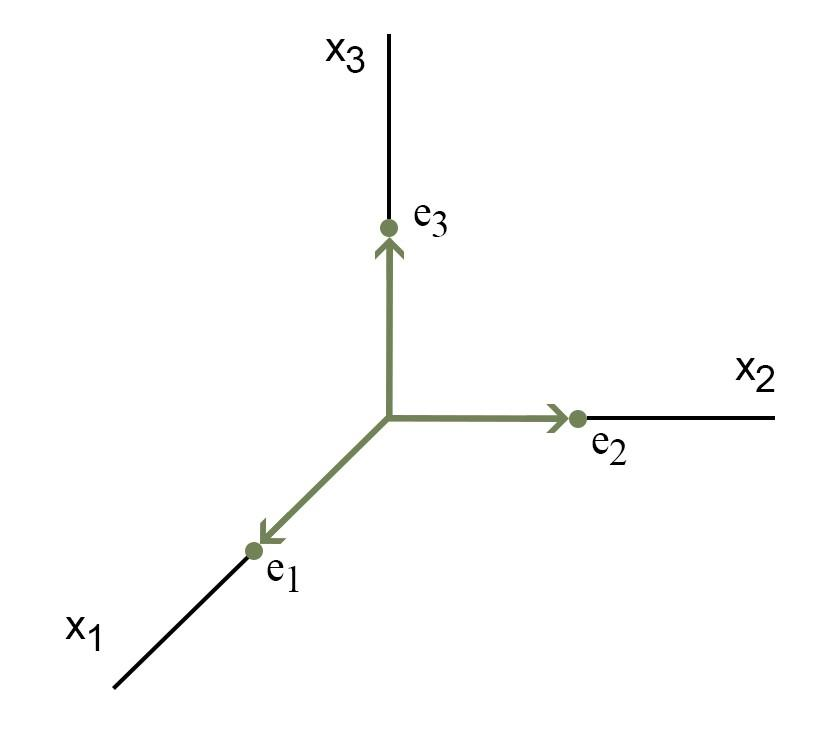
\includegraphics[width=0.50\textwidth]{Pictures/EVfig.4.jpg}
    \caption{Base canónica  de $\mathbb{R}^3$. }
    \label{EVfig. 4}
\end{figure}



\begin{example}
Dada una matriz $A$ de $m$ filas y $n$ columnas, y de rango $r$, todas las soluciones del sistema de ecuaciones homogéneo
$$A \vec{X}=\vec{0}, \qquad   \vec{X} \in \mathbb{R}^n$$
constituyen un subespacio vectorial de $\mathbb{R}^n$ generado por  $n-r$ vectores. Recordar que $r$ es la cantidad de pivotes al realizar operaciones elementales sobre las filas de la matriz  en eliminación gaussiana.

\bigskip
En el Ejemplo \ref{ejsistema} se tiene que  $m=3$, $n=4$ y el rango $r=3$. $S=Nul(A) = \langle (2,-1,-1,1) \rangle $,  es un subespacio de dimensión 
$n-r=4-3=1.$
\end{example}
\bigskip

\begin{example}

El conjunto $\left\{1,t,\cdots, t^{n}\right\}$ es una base de $P_K^{(n)}\left[t\right]$, ya que son polinomios linealmente independientes de acuerdo con el resultado del Ejemplo \ref{ejpk} (para $K= \mathbb{R}$), y todo polinomio $p$ de grado inferior o igual a $n$ puede escribirse de la forma
$$p(t)=a_01+a_1t+a_2t^{2} + \cdots +a_nt^{n}$$

 Para   para el caso $n=2$ se tiene la base $\left\{1,t, t^{2}\right\}$ que se muestra  en la Figura \ref{EVfig5}.
\end{example}
% figura base de P2

\begin{figure}
    \centering
    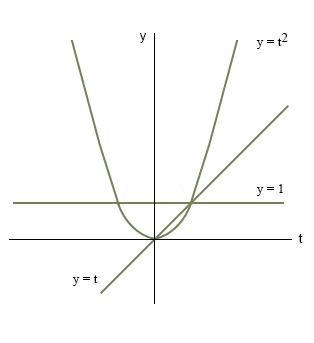
\includegraphics[width=0.50\textwidth]{Pictures/EVfig.5.jpg}
    \caption{Base canónica de $P_R^{(2)}\left[t\right]$ }
    \label{EVfig5}
\end{figure}

\bigskip

\begin{remark}
    El conjunto $\left\{1,t,\cdots, t^{n}\right\}$ no es una base de $P_K\left[t\right]$, ya que el polinomio $p(t)=t^{n+1}$ no es combinación lineal de estos. Se puede ver que ningún conjunto finito de polinomios  genera a $P_K\left[t\right]$ (ver  \cite{grossman}) .
%\hfill$\blacktriangle$
\end{remark}

\bigskip

\newpage

%\vskip0.5cm
\textbf{Coordenadas de un vector}\index{Coordenadas}

Si $\left\{\vec{e}_1,\vec{e}_2,\cdots, \vec{e}_n\right\}$ es una base de un espacio vectorial $V$ y $\vec{v}$ es cualquier elemento de $V$ podemos escribir a $\vec{v}$ como combinación lineal de $\vec{e}_1,\vec{e}_2,\cdots, \vec{e}_n$, de la forma

$$\vec{v}=  a_1\vec{e}_1+a_2\vec{e}_2+\cdots +a_n \vec{e}_n$$
con $a_j \in K$. Los números $a_1,a_2,\cdots,a_n$ se denominan \textit{coordenadas} de $\vec{v}$ con respecto a la base $\vec{e}_1,\vec{e}_2,\cdots, \vec{e}_n$.

\bigskip

\bigskip

\bigskip


\begin{theorem}
    
Las coordenadas de un vector $\vec{v}$ con respecto a una base son únicas.
 \begin{proof}
     Si suponemos se tienen  coordenadas $a_i$ y $b_i$, ~$i=1, \cdots n$ para un mismo vector $\vec{v}$,

$$\vec{v}=  a_1\vec{e}_1+a_2\vec{e}_2+\cdots +a_n \vec{e}_n$$
y 
$$\vec{v}=  b_1\vec{e}_1+b_2\vec{e}_2+\cdots +b_n \vec{e}_n$$
\noindent
se tiene  que 
$$\vec{0}=  (b_1-a_1)\vec{e}_1+(b_2-a_2)\vec{e}_2+\cdots +(b_n-a_n) \vec{e}_n$$
Como  $\vec{e}_1,\vec{e}_2,\cdots, \vec{e}_n$ son linealmente independientes,  $b_1=a_1$,  $b_2=a_2$, $\cdots$, $b_n=a_n$.
\end{proof}
\end{theorem}
%\vskip0.25cm

\bigskip



%\vskip1.5cm

\begin{example}


Sea $V=\mathbb{R}^{3}$    y sea $E$  la base canónica. Las coordenadas de un vector $\Vec{v}$ se anotan  $(x,y,z)_E=(x,y,z)$.


Si en lugar de la base canónica la base es $B=\left\{(1,1,1),(1,1,0),(1,0,0) \right\}$,  las coordenadas  de  un vector $(x,y,z)$  son $(z,y-z,x-y)_B$ y se escribe la igualdad $(x,y,z)=(z,y-z,x-y)_B$.

Esto se obtiene escribiendo  $(x,y,z)$ como combinación lineal de los vectores de $B$, $$(x,y,z)=a(1,1,1)+b(1,1,0)+c(1,0,0),$$ y  resolviendo el sistema lineal:

\begin{equation} 
\left\{ \begin{array} {ccl} \nonumber
                    a + b + c &\ =&x     \\
                     a + b + 0c &\ = &y  \\
                    a +0b +0c  &\ =&z \label{ejemplosist}
                   \end{array}
           \right.
\end{equation}


\end{example}

%coordenadas  ver ejemplos de la pag 22 


\bigskip

Un mismo espacio vectorial puede poseer varias bases; nuestro próximo objetivo es demostrar que todas ellas han de poseer el mismo número de elementos.

\bigskip

\begin{theorem}
\label{Prop1}
Si $V$ es un espacio vectorial que posee una base con $\textsl{n}$ elementos, cualesquiera $\textsl{n}+1$ vectores de $V$ son linealmente dependientes.

\bigskip
\begin{proof}


%\noindent
%\textsl{Demostración}

Sea $\left\{\vec{e}_1,\vec{e}_2,\cdots, \vec{e}_n\right\}$ una base de $V$ y sean $\vec{x}_1,\vec{x}_2,\cdots, \vec{x}_n, \vec{x}_{n +1} $,  $n+1$ vectores de $V$,

\bigskip
\noindent
que pueden escribirse como combinación lineal de la base dada:

\bigskip

$\vec{x}_1= \sum_{j=1}^{n} x_{j1}\vec{e}_j,  \qquad \vec{x}_2= \sum_{j=1}^{n} x_{j2}\vec{e}_j,  \qquad \vec{x}_n= \sum_{j=1}^{n} x_{jn}\vec{e}_j,   \qquad $ y $\vec{x}_{n+1}= \sum_{j=1}^{n} x_{jn+1}\vec{e}_j $

\bigskip


Se quiere ver si son linealmente independientes.  Nos preguntamos  si existen $a_i$ no todos nulos tales que 
  
  \bigskip
  
 $a_1\vec{x}_1+a_2\vec{x}_2+\cdots + a_n \vec{x}_n + a_{n+1}\vec{x}_{n +1} = \vec{0} $  
 
 \bigskip
 
Reemplazando, se  tiene

 \bigskip
 
 $   a_1  (\sum_{j=1}^{n} x_{j1}\vec{e}_j)  +  a_2  (\sum_{j=1}^{n} x_{j2}\vec{e}_j) +  a_n  (\sum_{j=1}^{n} x_{jn}\vec{e}_j) \\ + a_{n+1}  (\sum_{j=1}^{n} x_{j n+1}\vec{e}_j)= \vec{0}    $
 
  \bigskip
  
  Al desarrollar las sumas anteriores y  reordenar  sacando factor común los vectores $\vec{e}_j$,  se obtiene
  
  \bigskip
  
  
  $\vec{e}_1 ( x_{11}a_1+x_{12}a_2+ \cdots +x_{1n}a_n   +x_{1n+1}a_{n +1})=0  $
  
  \bigskip
  
  $\vec{e}_2 ( x_{21}a_1+x_{22}a_2+\cdots +x_{2n}a_n   +x_{2n+1}a_{n +1})=0  $
  
  \bigskip
  
  $\cdots$
  
   \bigskip
  
  $\vec{e}_n ( x_{n1}a_1+x_{n2}a_2+\cdots  +x_{nn}a_n   +x_{nn+1}a_{n +1})=0  $
  
  \bigskip
  
  Los términos entre paréntesis constituyen  un sistema homogéneo de $n$ ecuaciones con $n+1$ incógnitas, $a_1$, $a_2$,   $\cdots$, $a_{n+1}$ por lo que  existe  una solución no trivial ($a_i$ no todos nulos). 
  
  \bigskip
  
  Se concluye, entonces, que  los vectores $\vec{x}_1,\vec{x}_2,\cdots, \vec{x}_n, \vec{x}_{n +1} $ son lineal-\ mente dependientes.
  
  
  
  \end{proof}
\end{theorem} 

\bigskip


%\vskip1.5cm
\begin{remark}
De la proposición anterior se deduce un resultado un poco más general: en un espacio vectorial $V$ que posee una base con $n$ elementos, cualesquiera $m$ vectores de $V$, con $\textsl{m}>\textsl{n}$ son linealmente dependientes. Basta observar que $n+1$ de los $m$ vectores dados han de ser linealmente dependientes, debido a la proposición anterior, y por lo tanto, todos ellos han de formar un conjunto de vectores linealmente dependiente. Este resultado se aplica en la demostración del teorema que sigue.
%\hfill$\blacktriangle$
\end{remark}
%\vskip0.25cm

\bigskip

\bigskip

\bigskip

\index{Fourier, Jean-Baptiste.}
\begin{parchment}
[Jean-Baptiste Joseph Fourier (1768 - 1830)]{ Fue un matemático y físico francés conocido por sus trabajos sobre la descomposición de funciones periódicas en series trigonométricas convergentes llamadas Series de Fourier, método con el cual consiguió resolver la ecuación del calor. La transformada de Fourier recibe su nombre en su honor. Fue el primero en dar una explicación científica al efecto invernadero en un tratado.
Inició sus estudios en la Escuela Superior Benedictina de Auxerre, orientándose inicialmente a la carrera religiosa, hasta que el monarca Luis XV la convirtió en academia militar. Jean-Baptiste fue seleccionado como estudiante en la institución ya reformada, donde permanecería hasta los 14 años de edad, y empezó a ser instruido en idiomas, música, álgebra y matemáticas, materia en la que destacó, lo que le encaminó a dedicarse al estudio de las ciencias.
Posteriormente, participó en la Revolución francesa y, gracias a la caída del poder de Robespierre, se salvó de ser guillotinado. Se incorporó a la Escuela Normal Superior de París en donde tuvo entre sus profesores a los matemáticos Joseph Louis Lagrange y Pierre Simon Laplace. Posteriormente, ocupó una cátedra como docente en la prestigiosa École polytechnique.
Fourier participó en la expedición de Napoleón Bonaparte a Egipto en 1798. 
%Ya designado secretario perpetuo del Instituto de Egipto el 22 de agosto de 1798, presentó numerosas memorias y dirigió una de las comisiones de %exploración del Alto Egipto. Entre las distintas funciones políticas o administrativas que llevó a cabo, destaca la de comisario francés en el Divan. %A la muerte del General en Jefe del Ejército de Oriente Jean Baptiste Kléber a manos de un fanático sirio en su residencia en El Cairo, Fourier, %quien era amigo y colaborador del General Kléber, es designado para pronunciar el elogio fúnebre, el 17 de junio delante del Instituto de Egipto. A %su regreso a Francia en 1801, Napoleón Bonaparte le nombró prefecto de Isère y entre 1802 y 1815, Fourier presentó a Jean-François Champollion a los %veteranos de la expedición de Egipto.
Entró a la Academia de Ciencias Francesa en 1817 y al cabo de cinco años se convirtió en el secretario perpetuo de las secciones de matemáticas y física.
%Murió en París el 16 de mayo de 1830.
Fue en Grenoble donde condujo sus experimentos sobre la propagación del calor que le permitieron modelar la evolución de la temperatura a través de series trigonométricas. Estos trabajos mejoraron el modelado matemático de fenómenos físicos y contribuyeron a los fundamentos de la termodinámica.
Sin embargo, la simplificación excesiva que proponen estas herramientas fue muy debatida, principalmente por sus maestros Laplace y Lagrange.
Publicó en 1822 su Théorie analytique de la chaleur (Teoría analítica del calor), tratado en el cual estableció la ecuación diferencial parcial que gobierna la difusión del calor solucionándola mediante el uso de series infinitas de funciones trigonométricas, lo que establece la representación de cualquier función como series de senos y cosenos, ahora conocidas como las series de Fourier. El trabajo de Fourier provee el impulso para trabajar más tarde en las series trigonométricas y la teoría de las funciones de variables reales.
%Los dos primeros capítulos de la obra citada tratan problemas sobre difusión de calor entre cuerpos disjuntos en cantidad finita. 
Fourier en esta obra dedujo la ecuación en derivadas parciales que rige tal fenómeno, la cual es conocida como la ecuación del calor.  \cite{fourier}}
%En el capítulo III de la obra, titulado Difusión del calor en un cuerpo rectangular infinito Fourier introduce su método original de trabajo con %series trigonométricas.
\end{parchment}


\bigskip

\bigskip


\begin{theorem}
\label{2122}
%\textbf{PROPOSICIÓN 2.1.2.2 :}
Todas las bases de un mismo espacio vectorial $V$ poseen el mismo número de elementos.

\begin{proof}
Sean $\left\{\vec{e}_1,\vec{e}_2,\cdots, \vec{e}_n\right\}$  y $\left\{\vec{e}^{\prime}_1,\vec{ e}^{\prime}_2,\cdots, \vec{e}^{\prime}_m\right\}$ dos bases de un espacio vectorial $V$; por lo anterior $m\leq n$, ya que en caso contrario los vectores de la segunda base serían linealmente dependientes. Similarmente  \\ $n\leq m$
ya que en caso contrario los vectores de la primera base serían linealmente dependientes. Se tiene, por lo tanto, que $n=m$.

\end{proof}
\end{theorem}
%\vskip1.5cm

\bigskip


\index{Dimensión de un espacio vectorial}
El número de elementos que posee una base cualquiera de un espacio vectorial $V$ recibe el nombre de \textit{dimensión} de $V$; este número será designado mediante $dim(V)$. Si el espacio vectorial sólo contiene un elemento, es decir $V=\left\{\vec{0}\right\}$ tiene \textsl{dimensión cero}.

\bigskip


De los ejemplos anteriores podemos deducir los siguientes resultados:

\bigskip

\begin{enumerate}



\item

La dimensión de $K^{n}$  es $n$.
\item

La dimensión  de $P_K^{(n)}\left[t\right]$  es $n+1$.

\item
En el Ejemplo \ref{ejuis}  se puede ver que  $\bold{L}(\vec{u}_1,\vec{u}_2,  \vec{u}_3)$, donde $\vec{u}_1=(1,0,1)$, $\vec{u}_2=(-1,1,0)$ y $\vec{u}_3=(1,1,2)$,  es un subespacio vectorial de $\mathbb{R}^3$ de dimensión $2$ (un plano por el origen).

\end{enumerate}

\bigskip

\bigskip

\begin{remark}\index{Hiperplano}
    En $\mathbb{R}^n$ un \textit{hiperplano} que contiene al vector nulo es un subespacio $H$ de dimensión $n-1$. O sea  
    $$ H=\{ (x_1,x_2, \cdots, x_n): a_1x_1+a_2x_2 +  \cdots a_nx_n=0\}$$
\noindent
    donde $a_1, a_2, \cdots a_n$ son números reales fijos, no todos nulos. Es decir, un hiperplano  generaliza la noción de plano en $\mathbb{R}^3$.
\end{remark}

\bigskip

\begin{remark}
Se llama \textit{nulidad} de una matriz a la dimensión del espacio nulo. \index{Nulidad de una matriz}
\end{remark}
\bigskip

\begin{theorem}
\label{2123}

%\textbf{PROPOSICIÓN  2.1.2.3  :}

Sea $V$ un espacio vectorial de dimensión $n$. Todo conjunto de $n$ vectores de $V$ que sean linealmente independientes son una base de $V$.

\begin{proof}


Sean $\vec{x}_1,\vec{x}_2,\cdots, \vec{x}_n $,   $n$ vectores linealmente independientes. Si $\vec{v}$  es otro vector de $V$, por la Proposición  \ref{Prop1},   $ \vec{v}, \vec{x}_1,\vec{x}_2,\cdots, \vec{x}_n $  son linealmente dependientes.  
    
\bigskip

 Entonces, $\exists   \quad      a_0, a_1,  \cdots,  a_n$ tales que 

\bigskip

$ a_0 \vec{v} + a_1 \vec{x}_1+ a_2\vec{x}_2+ \cdots a_n \vec{x}_n = \vec{0}, \quad$   con algún $a_j$ no nulo.

\bigskip

En realidad $a_0$ debe ser no nulo, ya que si fuera $0$, los vectores $\vec{x}_1,\vec{x}_2,\cdots, \vec{x}_n $ serían linealmente dependientes. Se tiene, entonces, 
 
 
 



\[\vec{v} = \frac{-a_1}{a_0}  \vec{x}_1+\frac{-a_2}{a_0}  \vec{x}_2 \cdots a_n +\frac{-a_n}{a_0} \vec{x}_n \] 




\bigskip
\noindent
y por lo tanto $\vec{x}_1,\vec{x}_2,\cdots, \vec{x}_n $ generan $V$.

\end{proof}
\end{theorem}


\begin{remark}
Una forma sencilla de encontrar una base de un espacio vectorial $V$ es agregar vectores a un conjunto de vectores linealmente independientes de $V$. En la demostración de la proposición que sigue se explica la forma de agregarlos.
%\hfill$\blacktriangle$
\end{remark}
%\vskip0.25cm

\bigskip

\begin{theorem}
\label{2124}

Sea $V$ un espacio de dimensión finita $n$; todo conjunto de vectores linealmente independientes de $V$ puede completarse para obtener una base, es decir, dados $k$ vectores $\vec{e}_1,\vec{e}_2,\cdots, \vec{e}_k$, con $k<n$, de $V$, linealmente independientes, existen $n-k$ vectores $\vec{e}_{k+1},\vec{e}_{k+2},\cdots, \vec{e}_n$ de $V$ tal que el conjunto $\left\{\vec{e}_1,\vec{e}_2,\cdots, \vec{e}_k,\vec{e}_{k+1},\vec{e}_{k+2},\cdots, \vec{e}_n\right\}$ es una base de $V$.

\bigskip

\begin{proof}
Como $k<n$, puedo encontrar un elemento de $V$  linealmente indepen-\ diente con  $\vec{e}_1,\vec{e}_2,\cdots, \vec{e}_k$ (sino,  $ \left\{\vec{e}_1,\vec{e}_2,\cdots, \vec{e}_k  \right\}$ serían base de $V$). Lo llamo $\vec{e}_{k+1}$. Se repite con $ \left\{\vec{e}_1,\vec{e}_2,\cdots, \vec{e}_k, \vec{e}_{k+1}  \right\}$ hasta encontrar $n$ vectores linealmente independientes, que necesariamente serán base de $V$.
%\vskip1.5cm
\end{proof}
\end{theorem}

\bigskip

\noindent
Si $V$ es un espacio vectorial de dimensión finita $n$ en la Proposición \ref{2124} probamos  que $k$ vectores linealmente independientes de $V$ pueden \textit{completarse} para obtener una base. Puede demostrarse también  que si $S$ es un sistema de generadores de $V$, de él puede extraerse un subconjunto $S_1$ que sea una base de $V$.

%\vskip1.5cm
\bigskip
\noindent
Ahora unos comentarios acerca de la dependencia o independencia lineal de subconjuntos infinitos de un espacio  vectorial.

\bigskip

\begin{remark}
\begin{itemize}

\item 

\noindent
Un \textit{conjunto infinito} $S$ de elementos de un espacio vectorial $V$ se dice linealmente independiente si cualquier subconjunto finito de $S$ es linealmente independiente. En caso contrario, $S$ se dice \textit{linealmente dependiente}; es decir $S$ es linealmente dependiente si existe un subconjunto finito de él que es linealmente dependiente. 

%\vskip0.25cm
\item 
\noindent
Un espacio vectorial $V$ en el que se puede encontrar un subconjunto $S$ linealmente independiente y con infinitos elementos, se dice que tiene \textit{dimensión infinita
}.

\item 
\noindent
Los espacios  vectoriales $P_K\left[t\right]$, y $C(\left[0,2\pi\right])$, introducidos en la secciones anteriores, son espacios vectoriales de dimensión infinita. 
\item 
\noindent
El conjunto $S=\left\{t^{n}, n\in N\right\}$ es un conjunto linealmente independiente de $P_K\left[t\right]$ mientras que  el conjunto $S=\left\{cos(nx), sen(mx)\right\}_{n,m\in N}$ es un conjunto linealmente independiente en el espacio vectorial de las funciones continuas $C(\left[0,2\pi\right])$.
\end{itemize}
%\hfill$\blacktriangle$
\end{remark}






%\end{document}
\section{Intersección y suma de subespacios vectoriales}\index{Intersección de subespacios}\index{Suma de subespacios}
\label{intysumadesub}
Una pregunta que surge es si al considerar las operaciones de unión e intersección entre subespacios de un espacio vectorial $V$ (que son subconjuntos de $V$) se preserva la estructura de subespacio. Veremos que se preserva en la intersección pero no en la unión.

Dados dos subespacios $V_1$ y $V_2$ de un espacio vectorial $V$ podemos definir su \textit{intersección}

$$V_1\cap V_2=\left\{\vec{u},\vec{u}\in V_1 \wedge \vec{u}\in V_2\right\}$$
\noindent
y se demuestra fácilmente que $V_1\cap V_2$ es un subespacio.

Por otro lado, con un ejemplo se puede ver que con la unión de  dos subespacios $V_1$ y $V_2$, no ocurre lo mismo.   Si $V_1$ y $V_2$ son los subespacios generados por los vectores $(1,0)$ y $(0,1)$ (los ejes $x$ e $y$ respectivamente) la unión de $V_1$ y $V_2$ son los vectores  que están sobre un eje o el otro. $V_1\cup V_2$ no es un subespacio, ya que la suma no es cerrada: la suma de los vectores $(1,0)+(0,1)= (1,1) \notin V_1\cup V_2$ pues $(1,1) \notin V_1$ y $(1,1) \notin V_2$ siendo que $(1,0) \in V_1$ y $(0,1) \in V_2$.

Se define, entonces, para sí obtener un subespacio, la  \textit{suma} de dos subespacios $V_1$ y $V_2$ de la forma siguiente

$$V_1+V_2=\left\{\vec{u_1}+ \vec{u_2},\vec{u_1} \in V_1 \wedge \vec{u_2} \in V_2 \right\}$$
\noindent
y se puede demostrar  que $V_1+V_2$ es un subespacio vectorial de $V$ (y contiene a  $V_1\cup V_2$).

\bigskip

La relación que existe entre las dimensiones de estos subespacios vectoriales y las dimensiones de los subespacios $V_1$ y $V_2$ queda plasmada en el siguiente resultado:

\bigskip

\begin{theorem}
\label{2131}
$$dim(V_1 +V_2) =dim(V_1)+dim(V_2)- dim(V_1 \cap V_2) $$
para cualesquiera subespacios vectoriales $V_1$ y $V_2$ de un espacio vectorial $V$ de dimensión finita.

\begin{proof}


\noindent
Sea  $ \left\{\vec{e}_1,\vec{e}_2,\cdots, \vec{e}_l  \right\}$ una base de $V_1 \cap V_2$. Es posible completarla:


\bigskip

\noindent
 hasta obtener una base de $V_1$, $ \left\{\vec{e}_1,\vec{e}_2,\cdots, \vec{e}_l , \vec{f}_{l+1},\vec{f}_{l+2},\cdots, \vec{f}_k  \right\} $ 
 
 (de $l+(k-l)$ vectores)


\bigskip

\noindent
y también ,  hasta obtener una base de  $V_2$, 
$ \left\{\vec{e}_1,\vec{e}_2,\cdots, \vec{e}_l,  \vec{g}_{l+1},\vec{g}_{l+2},\cdots, \vec{g}_m  \right\}$   (de $l+(m-l)$ vectores).

\bigskip

%\noindent
Veremos que 

\bigskip
$ \left\{\vec{e}_1,\vec{e}_2,\cdots, \vec{e}_l ,\vec{f}_{l+1},\vec{f}_{l+2},\cdots, \vec{f}_k , \vec{g}_{l+1},\vec{g}_{l+2},\cdots, \vec{g}_m  \right\}$ 

es base de $V_1 +V_2$.


\bigskip

Está claro que es un sistema de generadores  de $V_1 +V_2$. Veamos que es un conjunto linealmente independiente. Se considera una combinación lineal igual al vector nulo:

\bigskip
\noindent
$a_1\vec{e}_1+a_2\vec{e}_2+\cdots+ a_l \vec{e}_l + b_{l+1} \vec{f}_{l+1}+ b_{l+2}\vec{f}_{l+2}+\cdots+ b_k \vec{f}_k +  c_{l+1}\vec{g}_{l+1}+c_{l+2}\vec{g}_{l+2}+\cdots+ c_m \vec{g}_m =  \vec{0} $

\bigskip
\noindent
que puede escribirse en forma equivalente 

\bigskip

\noindent
$a_1\vec{e}_1+a_2\vec{e}_2+\cdots+ a_l \vec{e}_l + b_{l+1} \vec{f}_{l+1}+ b_{l+2}\vec{f}_{l+2}+\cdots+ b_k \vec{f}_k =  -c_{l+1}\vec{g}_{l+1}-c_{l+2}\vec{g}_{l+2}-\cdots- c_m \vec{g}_m $

\bigskip


El término del lado izquierdo $\in V_1$, mientras que el lado derecho $\in V_2$. Es decir que está en $V_1 \cap V_2$ cuya base son los vectores $ \left\{\vec{e}_1,\vec{e}_2,\cdots, \vec{e}_l  \right\}$. Entonces es posible escribir el término de la derecha como combinación lineal de la base $ \left\{\vec{e}_1,\vec{e}_2,\cdots, \vec{e}_l  \right\}$ con coordenadas $\delta_i$.  Es decir, se tiene la igualdad 

\bigskip


$-c_{l+1}\vec{g}_{l+1}-c_{l+2}\vec{g}_{l+2}-\cdots- c_m \vec{g}_m =   \delta_1\vec{e}_1+\delta_2\vec{e}_2+\cdots+ \delta_l \vec{e}_l   $

\bigskip
\noindent
que puede reescribirse,


\bigskip

$\delta_1\vec{e}_1+\delta_2\vec{e}_2+\cdots+ \delta_l \vec{e}_l + c_{l+1}\vec{g}_{l+1}+c_{l+2}\vec{g}_{l+2}+\cdots+ c_m \vec{g}_m= \vec{0}$

\bigskip

Por ser  $ \left\{\vec{e}_1,\vec{e}_2,\cdots, \vec{e}_l ,  \vec{g}_{l+1},\vec{g}_{l+2},\cdots, \vec{g}_m  \right\}$ una base de $V_2$, se tiene que 

\bigskip

$ c_{l+1}=c_{l+2}=\cdots= c_m  =   \delta_1=\delta_2=\cdots+ \delta_l=0   $

\bigskip

\noindent
y, entonces, el término de la izquierda, 

\bigskip

$a_1\vec{e}_1+a_2\vec{e}_2+\cdots+ a_l \vec{e}_l + b_{l+1} \vec{f}_{l+1}+ b_{l+2}\vec{f}_{l+2}+\cdots+ b_k \vec{f}_k=  \vec{0} $

\bigskip

\noindent
y como $ \left\{\vec{e}_1,\vec{e}_2,\cdots, \vec{e}_l , \vec{f}_{l+1},\vec{f}_{l+2},\cdots, \vec{f}_k  \right\} $ son base de $V_1$,  son linealmente independientes, 

\bigskip

 $a_1=a_2=\cdots+ a_l = b_{l+1}=b_{l+2}=\cdots= b_k =0$

\bigskip

\newpage
Luego,

\bigskip

$dim(V_1 +V_2)=l + (k-l) + (m-l) = k+m-l 

=dim(V_1)+dim(V_2)-dim(V_1 \cap V_2)$
\end{proof}
\end{theorem}

\bigskip
%\vskip0.25cm



\begin{remark}
\begin{itemize}
    \item 

 Si $V_1$ y $V_2$ son los subespacios generados por los vectores $(1,0)$ y $(0,1)$ respectivamente, la suma de $V_1$ y $V_2$ da todo $\mathbb{R}^2$, ya que $(x,y)= (x,0) + (0,y)$, $(x,0) \in V_1$ y $(0,y) \in V_2$.
 \item 
Es importante notar que $V_1+V_2$ es el menor subespacio (con respecto a la inclusión) que contiene a $V_1\cup V_2$.
\end{itemize}
%\hfill$\blacktriangle$
\end{remark}

%\vskip0.25cm
\bigskip

\begin{example}
%$S=\{ (x_1,x_2,\cdots, x_n) \in K^n, a_1.x_1+a_2.x_2+\cdots +a_n.x_n=0,\}$
El subespacio $S$ de las soluciones del sistema homogéneo, 
\begin{equation} 
S=\{ (x_1,x_2,\cdots, x_n) \in K^n
\left\{ \begin{array} {rcl} \nonumber
               a_{11}x_1+a_{12}x_2+\cdots +a_{1n}x_n& =&0\\
               \cdots \\
                    a_{m1}x_1+a_{m2}x_2+\cdots +a_{mn}x_n& =&0
                   \end{array}
           \right.
           \label{ejsist}
\end{equation}
es un subespacio de $K^n$. Es  intersección de $m$ subespacios,  $S=\bigcap^{m}_{i=1} S_i$, donde $S_i=\{ (x_1,x_2,\cdots, x_n) \in K^n, a_{i1}x_1+a_{i2}x_2+\cdots +a_{in}x_n=0,\}, 1\leq i\leq m$. Cada $S_i$ es un subespacio de $K^n$ (correspondiente a las soluciones de cada una de las $m$ ecuaciones, como se vió en el  Ejemplo \ref{ejintsub}, Sección  \ref{Subespacio vectorial}).
\end{example}


\begin{example}



Dos subespacios vectoriales distintos de $\mathbb{R}^{2}$,  $V_1$ y $V_2$, ambos de dimensión $1$, tienen una suma que coincide con todo $\mathbb{R}^{2}$, ya que 

$$dim(V_1 +V_2)=dim(V_1)+dim(V_2)-dim(V_1 \cap V_2)=1 + 1 -0=2 $$

\end{example}


\begin{definition}\index{Suma directa}


Un espacio vectorial $V$ es \textit{suma directa} de dos subespacios $V_1$ y $V_2$ si 

\begin{enumerate}

\item $V_1 +V_2=V$

\item $V_1 \cap V_2={\vec{0}}$



\end{enumerate}
\end{definition}
Utilizaremos la notación $V=V_1 \oplus V_2$ para indicar que $V$ es suma directa de los subespacios $V_1$ y $V_2$.


\bigskip

\begin{remark}
\begin{itemize}




\item 

El plano $\mathbb{R}^{2}$ puede escribirse como suma directa de dos rectas no coincidentes que pasan por el origen.

\item El espacio $\mathbb{R}^{3}$ puede escribirse como suma directa de un plano que pasa por el origen y una recta que le corta en ese punto.

\item De acuerdo a la Proposición \ref{2131} anterior  si $V=V_1 \oplus V_2$, se tiene que 

$$dim(V)=dim(V_1 \oplus V_2)=dim(V_1)+dim(V_2)$$
ya que el subespacio $V_1 \cap V_2={\vec{0}}$ tiene dimensión $0$. Además, si $B_1$ es base de $V_1$ y $B_2$ es base de $V_2$, $B=B_1\cup B_2$ es una base de $V$.

\end{itemize}
%\hfill$\blacktriangle$
\end{remark}

\bigskip

\begin{example}
Sean los subespacios de $\mathbb{R}^3$, 
$S=\{ \vec{x} \in \mathbb{R}^3, x_1+x_2+x_3=0,\}$ y $T=\left\langle (1,1,1)\right\rangle$. Se tiene que $dim(S)=2$, $dim(T)=1$ y $S\cap T={\vec{0}}$. 
Entonces, $dim(S+T)=3$, de donde,  $S+T=\mathbb{R}^3$.
\end{example} 


\begin{remark}
Si $V=V_1 +V_2$ todo elemento $\vec{v}\in V$ puede escribirse de la forma $\vec{v}=\vec{v}_1+\vec{v}_2$ con $\vec{v}_1 \in V_1$ y $\vec{v}_2 \in V_2$. Si la suma es directa, esta descomposición es única. 
%\hfill$\blacktriangle$
\end{remark}


 \bigskip

%\newpage


\begin{theorem}
\label{2132}
Sean  $V_1$ y $V_2$  subespacios vectoriales de un espacio vectorial $V$. Las siguientes afirmaciones son equivalentes:

\begin{enumerate}

\item 

$V=V_1  \oplus V_2$

\item 
Para todo $\vec{v}\in V$  existe una descomposición  única de la forma 

$\vec{v}=\vec{v}_1+\vec{v}_2$ con $\vec{v}_1 \in V_1$ y $\vec{v}_2 \in V_2$.  

  
\end{enumerate}

\begin{proof} 
Veamos que $1 \rightarrow  2$

Supongamos $\vec{v}=\vec{v}_1+\vec{v}_2$ con $\vec{v}_1 \in V_1$ y $\vec{v}_2 \in V_2$  y $\vec{v}=\vec{u}_1+\vec{u}_2$ con $\vec{u}_1 \in V_1$ y $\vec{u}_2 \in V_2$. 

\bigskip
Se tiene que, 
$$\vec{v}_1+\vec{v}_2  = \vec{u}_1+\vec{u}_2, $$
\noindent
igualdad que puede reescribirse

$$\vec{v}_1-\vec{u}_1  = \vec{u}_2-\vec{v}_2 $$

De donde $\vec{v}_1-\vec{u}_1$ $\in  V_1 \cap V_2 $, como por hipótesis,      $V_1 \cap V_2={\vec{0}}$, $\vec{v}_1=\vec{u}_1 $ y de la misma forma, $\vec{v}_2=\vec{u}_2 $.

\noindent
Para ver que  $2 \rightarrow  1$ alcanza con demostrar que $V_1 \cap V_2={\vec{0}}$.

Si $ \vec{v} \in  V_1 \cap V_2={\vec{0}}$, $ \vec{v} $ se puede escribir $ \vec{v}=\vec{v}+  \vec{0}  $ y $ \vec{v}=\vec{0}+  \vec{v}  $,
\noindent
como la descomposición es única, $ \vec{v}= \vec{0} $.

\end{proof}
\end{theorem}


\bigskip

%También podemos definir la intersección, la suma y la suma directa de más de dos subespacios vectoriales. 





En general, dados $n$ subespacios vectoriales $V_1, V_2, \cdots, V_n$ de un espacio vectorial $V$, definimos

$$\bigcap^{n}_{j=1}V_j=\left\{\vec{u}\in V, \vec{u}\in V_j, j=1,\cdots,n\right\}$$
\noindent
y

$$\sum^{n}_{j=1}V_j=\left\{\sum^{n}_{j=1}\vec{u_j},~ \vec{u_j}\in V_j,j=1,\cdots,n\right\}$$

\bigskip
\noindent
que reciben el nombre de \textit{intersección} y \textit{suma}, respectivamente, de los subespacios vectoriales $V_j$ dados. Estos dos nuevos subespacios son también subespacios vectoriales de $V$.



La definición de \textsl{suma directa} de varios subespacios vectoriales es un poco más complicada en general, que si solamente hay dos. Se dice  que $V$ es \textsl{suma directa}  de los subespacios vectoriales  $V_1, V_2, \cdots, V_n$ y se escribe
$$ V= V_1 \oplus V_2 \oplus V_3 \oplus \cdots \oplus V_n$$
si todo vector  $\vec{v}\in V$  tiene  una descomposición \textsl{ única} de la forma $\vec{v}=\sum^{n}_{i=1} \vec{v_i}$ con $\vec{v_i} \in V_i, i=1,\cdots, n $.  


%\vskip1.5cm

\begin{remark}
\label{obssumadesub}
\begin{itemize}

\item
Si $n=2$, esta última definición y la dada anteriormente son equivalentes. 

\item
Para $n\geq 3$ se puede demostrar que las siguientes afirmaciones son  equivalentes:

\begin{itemize}
\item
$ V= V_1 \oplus V_2 \oplus V_3 \oplus \cdots \oplus V_n$

\item

$V= \sum^{n}_{i=1}V_i$ y $V_i\cap(\sum^{n}_{k \neq i}V_k)={\vec{0}}$

\end{itemize}

\end{itemize}
%\hfill$\blacktriangle$
\end{remark}




\section{ Cambio de base}\index{Matriz de cambio de base}
\label{Cambio de base}

\begin{figure}
    \centering
    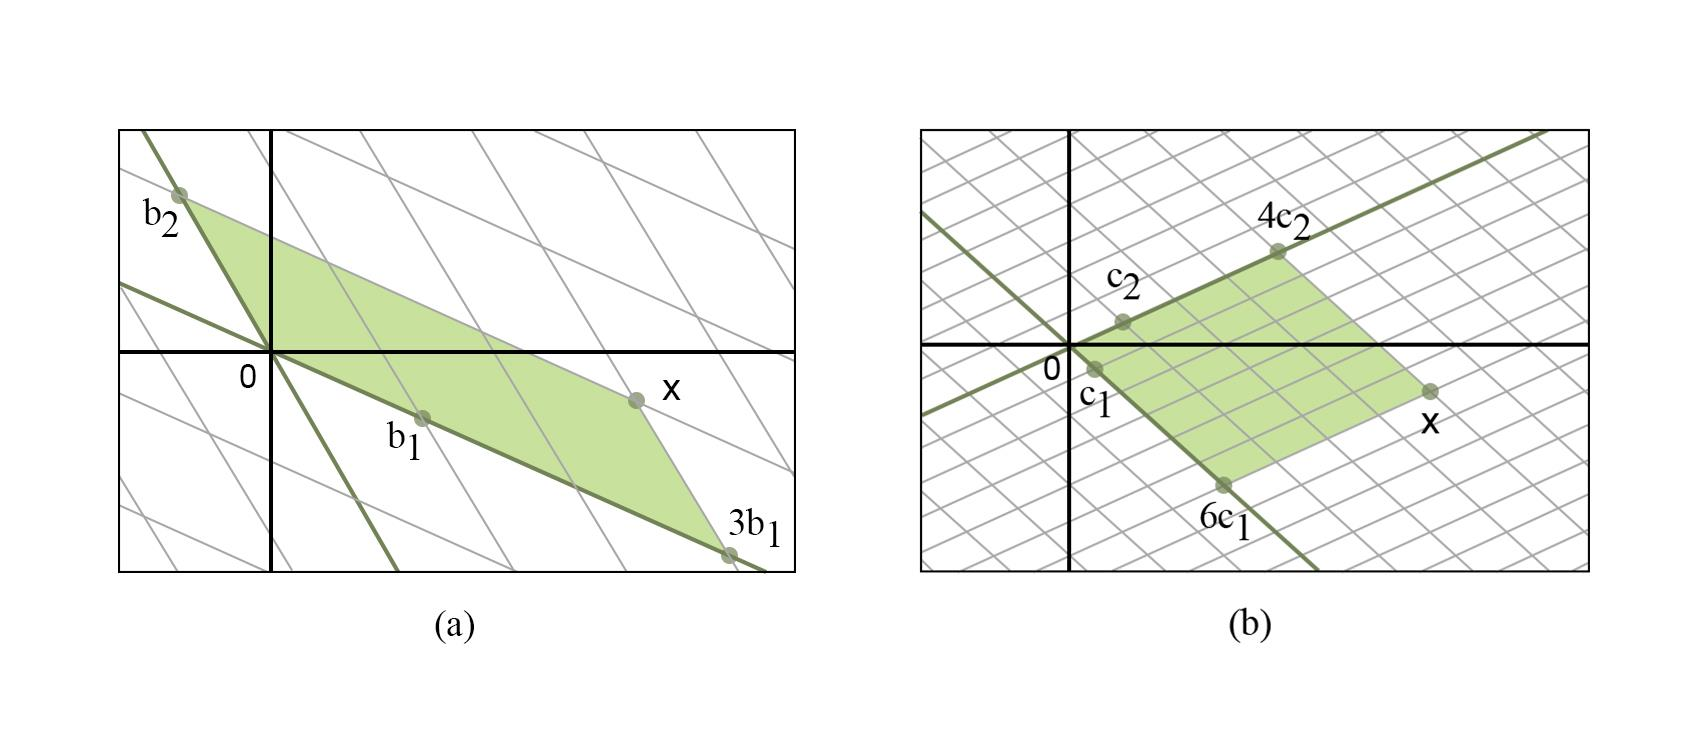
\includegraphics[width=0.99\textwidth]{Pictures/TLfig80.jpg}
    \caption{Coordenadas de un vector $\vec x$, en las bases $\{\vec b_1,\vec b_2\}$ (a) y $\{\vec c_1,\vec c_2\}$ $(b)$}
    \label{TLfig700}
\end{figure}


Para visualizar el problema de cambio de base, considere los dos  sistemas de  coordenadas que se muestran en
la Figura \ref{TLfig700}.  En $(a)$, $\vec{x} = 3\vec{b}_1 +1 \vec{b}_2$, mientras que en $(b)$, el mismo vector $\vec{x}$ se
expresa como $\vec{x} = 6\vec{c}_1 +4 \vec{c}_2$. 
%Esto es,
%[ x ]B = 3
%1
%y [ x ]C = 6
%4
El problema consiste en encontrar la relación que hay entre las coordenadas de un mismo vector $\vec{x}$ en las dos bases  $  \{\vec{b}_1,\vec{b}_2 \}$  y $  \{\vec{c}_1,\vec{c}_2 \}$ .
%En el ejemplo 1 se muestra cómo hacer esto, suponiendo que ya se sabe cómo
%están formadas b1 y b2 a partir de c1 y c2.



Para el caso general, supongamos que se tienen dos bases  $B$ y $B ^{\prime}$ de un espacio vectorial $V$ de dimensión finita. Se verá que con la ayuda de una matriz se pueden obtener las coordenadas de un vector con respecto a una base de $V$ a partir de las coordenadas del vector en la  otra base. Llamaremos base antigua a la base $B$ y base nueva a la base $B ^{\prime}$.


Si $B =\left\{\vec{e_1},\vec{ e_2},\cdots, \vec{e_m}\right\}$ y $B ^{\prime}=\left\{\vec{e}^{\prime}_1,\vec{e} ^{\prime}_2,\cdots, \vec{e} ^{\prime}_m\right\}$ son dos bases de un espacio vectorial $V$ de dimensión $n$,
todo elemento de la base  $B ^{\prime}$   puede escribirse como combinación lineal de los elementos de la base $B$ :

\begin{equation} \label{matriz Acb}
\left\{ \begin{array} {ccl} 
                    \vec{e }^{\prime}_1&\ =&   a_{11}\vec{e}_1+a_{21}\vec{e}_2+\cdots +a_{n1}\vec{e}_n    \\
                     \vec{e }^{\prime}_2 &\ = &a_{12}\vec{e}_1+a_{22}\vec{e}_2+\cdots +a_{n2}\vec{e}_n  \\
										\cdots  \\
                    \vec{e }^{\prime}_n &\ =&a_{1n}\vec{e}_1+a_{2n}\vec{e}_2+\cdots +a_{nn}\vec{e}_n
                   \end{array}
           \right.
\end{equation}


\bigskip

\noindent
que en forma abreviada puede escribirse


$$\vec{e }^{\prime}_j=\sum^{n}_{i=1}a_{ij}\vec{e}_i, \qquad j=1, \cdots n$$

\begin{remark}
Puede escribirse en forma más concisa  usando convenio de Einstein (índice repetido indica suma)
$$  \vec{e }^{\prime}_j=a_{ij}\vec{e}_i, \qquad  j=1, \cdots n  $$
%\hfill$\blacktriangle$
\end{remark}

\bigskip


La nueva  base $B ^{\prime}$   se obtiene de la base $B$ mediante la siguiente matriz 



$$A=\left(\begin{array}{cccc} a_{11} & a_{12}&  \cdots & a_{1n} \\a_{21}  & a_{22} & \cdots & a_{2n}
\\  \cdots & \cdots  &  \cdots  & \cdots \\ a_{n1} & a_{n2} & \cdots & a_{nn}
\end{array}
 \right)$$
 \bigskip
\noindent
donde la $j$-ésima columna de $A$ son las coordenadas del vector $\vec{e }^{\prime}_j$ con respecto a la base antigua $\vec{e}_j$, $j=1,2,\cdots ,n$.

\bigskip

 La matriz $A$ se denomina \textsl{matriz del cambio de base}  de   $B ^{\prime}$ a $B$ y se denota $P_{B, B^{\prime}}$.

\begin{remark}
\begin{itemize}
\item
A la matriz del cambio de base  de   $B ^{\prime}$ a  $B$ también se la denomina  \textsl{matriz de transición}  de la base   $B ^{\prime}$ a la base  $B$.
\item
 Cuando  sea necesario hacer constar las bases $B$ y $B ^{\prime}$ escribiremos $P_{B^{\prime},B}$ para denotar la matriz de cambio de base de  $B$ a $B ^{\prime}$. 

\item
Si $B$ y $B ^{\prime}$ coinciden se tiene que $P_{B ^{\prime},B}=I_{n {\times}n}$.
\end{itemize}
%\hfill$\blacktriangle$
\end{remark}



\begin{theorem}
\label{2141}
La matriz $A$ del cambio de base de  $B ^{\prime}$  a $B$  es invertible  y su inversa es la matriz de cambio de base de $B$ a  $B ^{\prime}$. Podemos,  por lo tanto, escribir

$$A^{-1}=P_{B,B ^{\prime}}^{-1}= P_{B ^{\prime},B}$$

\begin{proof} 

\noindent 
El determinante de la matriz es no nulo, ya que sus columnas son las coordenadas de los vectores $ \vec{e }_j $ que por ser una base son linealmente independientes.

\bigskip




Si  $A^{\prime}$ es la matriz de cambio de base de $B$ a $B^{\prime}$, entonces  se tiene 


$$\vec{e }_j=\sum^{n}_{i=1}a_{ij}^{\prime} \vec{e}^{\prime}_i, \qquad j=1, \cdots n$$

 


\bigskip
\noindent
 y por la definición de la matriz $A$,

 $$\vec{e }^{\prime}_i=\sum^{n}_{k=1}a_{ki} \vec{e}_k, \qquad i=1, \cdots n.$$
\noindent 
 por lo tanto, 

 \bigskip
 
$\vec{e }_j=\sum^{n}_{i=1}a_{ij}^{\prime} (   \sum^{n}_{k=1}a_{ki} \vec{e}_k)=\sum^{n}_{k=1}  (   \sum^{n}_{k=1}a_{ki}   a_{ij}^{\prime} ) \vec{e}_k, \qquad j=1, \cdots n.$


\bigskip


\noindent 
Como el término dentro de la sumatoria en $k$, $ \sum^{n}_{k=1}a_{ki}   a_{ij}^{\prime} $, es el elemento que ocupa el lugar $(k,j)$ del producto de las matrices $A$ y $A^{\prime}$,  de acuerdo a la igualdad, ese término   vale $1$ si $k=j$, y $0$ si no. Es decir que se tiene que el producto de las matrices  $A$ y $A^{\prime}$, es   $AA^{\prime}=I_{n \times n}$.

\end{proof}
\end{theorem}

\bigskip


\bigskip

\begin{remark}

\begin{itemize}



\item
Las expresiones anteriores pueden reescribirse en forma sintética  considerando que el índice repetido se suma de $1$ a $n$: 
$ \vec{e }_j=  a_{ij}^{\prime}  \vec{e}_i^{\prime}$

\bigskip

\item
Usando la delta de Kronecker,  $ \delta_{kj}$ (definida  $ \delta_{kj}=1$ si $k=j$ y $ \delta_{kj}=0$ si $k\neq j$),

\noindent
la expresión se escribe $ \vec{e }_j=a_{ki}  a_{ij}^{\prime}  \vec{e}_k= \delta_{kj}\vec{e}_k$
\end{itemize}
%\hfill$\blacktriangle$
\end{remark}


\bigskip


\begin{example}
\label{cambiob1}
Dadas las bases de  $\mathbb{R}^{3}$, $B =\left\{(1,1,1), (1,1,0),(1,0,0)\right\}$ y $B^{\prime}= \left\{\vec{e}_1,\vec{e}_2, \vec{e}_3\right\}$  (base canónica), la matriz de cambio de base de $B$ a $B^{\prime}$,  de acuerdo a las Ecs.(\ref{matriz Acb}), es


%\vskip1.25cm

$$P_{B ^{\prime},B}=\left(\begin{array}{ccc} 1 & 1 &  1 \\ 1 & 1 & 0
\\ 1 & 0 & 0
\end{array}
 \right)$$
\end{example}

\begin{remark}
\label{cambiobasecan}
Si la base nueva, $B^{\prime}$ es la base la canónica, la matriz de cambio de base de $B$ a $B^{\prime}$ se obtiene directamente  poniendo las coordenadas de los vectores de la base $B$ en cada columna  (ver Ejemplo \ref{cambiob1}).
%\hfill$\blacktriangle$
\end{remark}




\textbf{Relación entre las coordenadas en la base $B$ y en la $B^{\prime}$}
\label{RELCOORD}

\bigskip

\noindent 
Tratemos ahora de relacionar entre sí las coordenadas de un mismo vector en las bases nueva $B ^{\prime}$  y antigua $B$. Supongamos que $\vec{x}\in V$,


    
\begin{equation}
\label{ecx}
\vec{x}= x_1\vec{e}_1+x_2\vec{e}_2+\cdots +x_n\vec{e}_n 
\end{equation}

\noindent 
y además
\begin{equation}
\label{ecxp}
\vec{x}= x^{\prime}_1\vec{e}^{\prime}_1+x^{\prime}_2\vec{e}^{\prime}_2+\cdots +x^{\prime}_n\vec{e}^{\prime}_n 
\end{equation}

\bigskip

\noindent 
Sustituyendo Ec.(\ref{matriz Acb}) en la segunda expresión, Ec.(\ref{ecxp}), obtenemos

\bigskip

$$\vec{x}= x_1^{\prime} ( \sum^{n}_{i=1}  a_{i1} \vec{e}_i)+x_2^{\prime}( \sum^{n}_{i=1}  a_{i2} \vec{e}_i)+\cdots +x_n^{\prime}( \sum^{n}_{i=1}  a_{in} \vec{e}_i)$$

\bigskip

$$=(a_{11}x_1^{\prime}+  a_{12}x_2^{\prime}  +\cdots + a_{1n}x_n^{\prime}  )\vec{e}_1+ (a_{21}x_1^{\prime}+  a_{22}x^{\prime}_2  +\cdots$$


$$+ a_{2n}x_n^{\prime}  )   \vec{e}_2+\cdots +   (a_{n1}x_1^{\prime} +  a_{n2}x_2^{\prime}   +\cdots + a_{nn}x_n^{\prime}   )\vec{e}_n$$

\bigskip


Comparando esta última igualdad con la primera expresión Ec.(\ref{ecx}) podemos escribir 

\begin{equation} \label{ec4}
\left\{ \begin{array} {ccl} 
                    x_1&\ =&   a_{11}x_1^{\prime}+a_{12}x_2^{\prime}+\cdots +a_{1n}x_n^{\prime}    \\
                     x_2 &\ = &a_{21}x_1^{\prime}+a_{22}x_2^{\prime}+\cdots +a_{2n}x_n^{\prime}  \\
										\cdots  \\
                    x_n &\ =&a_{n1}x_1^{\prime}+a_{n2}x_2^{\prime}+\cdots +a_{nn}x_n^{\prime}
                   \end{array}
           \right.
\end{equation}

%\vskip1.25cm

Si convenimos en escribir $X=\left(\begin{array}{c} x_{1} \\ x_{2}  
\\  x_3 \\ \cdots \\ x_{n} 
\end{array}
 \right)$ y $X^{\prime}=\left(\begin{array}{c} x^{\prime}_{1} \\ x^{\prime}_{2}  
\\  x^{\prime}_3 \\ \cdots \\ x^{\prime}_{n} 
\end{array}\right)$ 

\bigskip
\noindent
a las coordenadas del vector $\vec{x}$ en la antigua base  $B$  y en la nueva base $B ^{\prime}$ , respectivamente, las Ecs.(\ref{ec4}) se escribe  de la forma

%\vskip1.25cm
\begin{equation}
\label{XPAX}
X=AX^{\prime}
\end{equation}

Esto  permite obtener las coordenadas del vector $\vec{x}$ en la base antigua  conociendo las coordenadas del mismo vector en la  base nueva.

%\vskip1.25cm



\begin{example}


Dadas las mismas  bases del Ejemplo \ref{cambiob1}, 

$B =\left\{(1,1,1), (1,1,0),(1,0,0)\right\}$ y $B^{\prime}= \left\{\vec{e}_1,\vec{e}_2, \vec{e}_3\right\}$, se quieren encontrar las coordenadas del vector $\vec{x}=(3,2,3)_{B^{\prime}}$ en la base $B$, para lo cual se necesita la matriz de cambio de base, $P_{B,B ^{\prime}}$.

De acuerdo a las Ecs. (\ref{matriz Acb}), la matriz de cambio de base, $P_{B,B ^{\prime}}$ se obtiene a partir de encontrar las coordenadas de  los vectores de la base $B^{\prime}$ en la base $B$  y colocarlos como columnas. Después de resolver el sistema de ecuaciones se obtuvo



\begin{equation} \label{ec5}
\left\{ \begin{array} {ccl} 
                   (1,0,0)&\ =&   0 (1,1,1)+0(1,1,0)+1(1,0,0)   \\
									(0,1,0)&\ =&   0 (1,1,1)+1(1,1,0)+(-1)(1,0,0)   \\
									(0,0,1)&\ =&   1 (1,1,1)+(-1)(1,1,0)+0(1,0,0)
                    \end{array}
           \right.
\end{equation}

\bigskip
\noindent
y entonces, 

\bigskip

$$P_{B,B ^{\prime}}=\left(\begin{array}{ccc} 0 & 0 &  1 \\ 0 & 1 & -1
\\ 1 & -1 & 0
\end{array}
 \right)$$
 
\bigskip

 Otra alternativa para hallar la matriz $P_{B,B ^{\prime}}$   es usar la Proposición \ref{2141} y entonces  $  P_{B,B ^{\prime}} = P_{B ^{\prime},B}^{-1}$ dado que $P_{B ^{\prime},B}$ se encontró en el Ejemplo \ref{cambiob1}.

\bigskip

Luego, usando (\ref{XPAX}), las coordenadas son

\bigskip

$$X=P_{B,B ^{\prime}}X^{\prime}=\left(\begin{array}{ccc} 0 & 0 &  1 \\ 0 & 1 & -1
\\ 1 & -1 & 0
\end{array}
 \right) \left(\begin{array}{c} 3 \\ 2  
\\ 3  
\end{array} \right)_{B ^{\prime}} =\left(\begin{array}{c} 3 \\ -1 
\\ 1  
\end{array} \right)_{B}$$

\bigskip

Así se obtuvieron  las coordenadas del vector $\vec{x}$ en la base  $B$ conociendo las coordenadas del mismo vector en la base $B ^{\prime}$.
\end{example}


\bigskip


\bigskip

\begin{example}
\label{ejrotR2}

Sean $\vec{e}_1$ y $\vec{e}_2$ dos vectores perpendiculares unitarios en $\mathbb{R}^{2}$ en la dirección de los ejes de coordenadas cartesianas. Girando los ejes de coordenadas un ángulo $\phi$ en sentido positivo, contrario a las agujas del reloj, se obtiene una nueva base  $B ^{\prime}=\{ \vec{e}_1^{\prime}$, $\vec{e}_2^{\prime}\}$.

\bigskip


\bigskip

De acuerdo a la Figura \ref{EVrot}, se observa que 


\begin{equation} \label{rot}
\left\{ \begin{array} {ccl} 
                    \vec{e}^{\prime}_1&\ =&   cos(\phi)\vec{e}_1+sen(\phi)\vec{e}_2    \\
                     \vec{e}^{\prime}_2 &\ = &-sen(\phi)\vec{e}_1+ cos(\phi)\vec{e}_2 \\
										
                   \end{array}
           \right.
\end{equation}

\bigskip
\noindent
por lo cual, teniendo en cuenta el sistema (\ref{matriz Acb}),  la matriz del cambio de base $A$ es 


\begin{equation}
\label{matrizrotR2}
A= \left(\begin{array}{cc}  cos(\phi) & -sen(\phi)  \\ sen(\phi) &  cos(\phi)
\end{array}
 \right)
\end{equation}

\begin{figure}
    \centering
    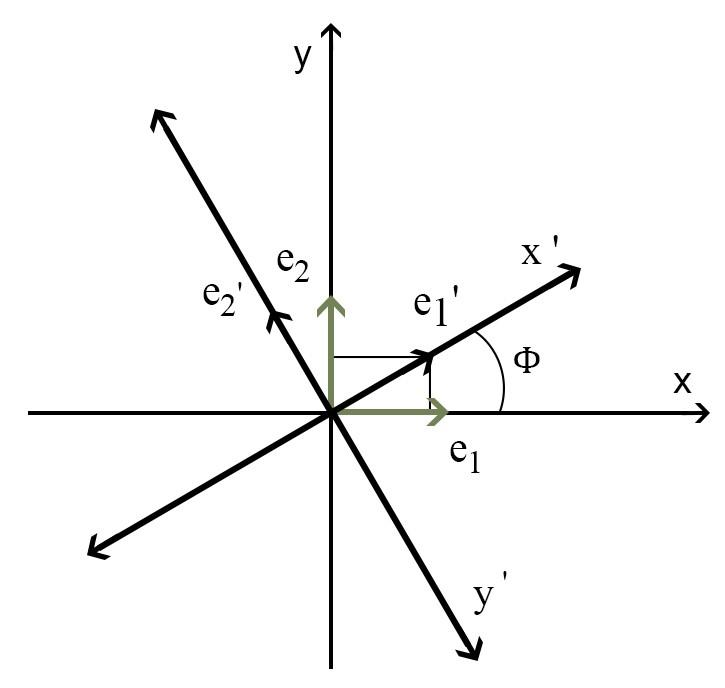
\includegraphics[width=0.60\textwidth]{Pictures/EVrot.jpg}
    \caption{Cambio de base. Rotación de ejes en un ángulo $\phi$.}
    \label{EVrot}
\end{figure}

\bigskip

Así, si $\phi= \pi/4$, las coordenadas respecto a la base $B=\{ \vec{e}_1^{\prime}$, $\vec{e}_2^{\prime} \}$ del vector $(2,3)_B$

\bigskip


$$\left(\begin{array}{cc}  cos(\pi/4) & -sen(\pi/4)  \\ sen(\pi/4) &  cos(\pi/4)
\end{array}
 \right)^{-1}\left(\begin{array}{c}  2 \\ 3
\end{array}
 \right)_{B}\approx \left(\begin{array}{c}  3.53 \\ 0.71
\end{array}
 \right)_{B ^{\prime}} $$
\end{example}


\bigskip

\bigskip

\begin{example}
Dadas las bases de $P_\mathbb{R}^{(2)}\left[x\right]$, $B =\left\{3,1+x,x^{2}\right\}$  y $B^{\prime}= \left\{1,x+3,x^{2}+x\right\}$, se quiere hallar la matriz de cambio de base de $B ^{\prime}$ a $B$.

Teniendo en cuenta la Observación {\textcolor{blue}{\fontfamily{qcr}\selectfont{i}}}, luego del Ejemplo \ref{cambiob1} resulta más simple hallar $P_{E,B}$ y  $P_{E,B ^{\prime}}$, donde $E =\left\{1,x,x^{2}\right\}$ es la base canónica.
 Como 


\begin{eqnarray*}
1&= & 1\cdot 1+0 \cdot x+ 0 \cdot x^2 \\
x+3&= &3\cdot1+ 1\cdot x +  0\cdot x^2 \\
x^2+x & = &0\cdot 1+ 1\cdot x + 1\cdot x^2
\end{eqnarray*}

Se tiene  que  
$$P_{E,B ^{\prime}}=\left(\begin{array}{ccc} 1 & 3 &  0 \\ 0 & 1 & 1
\\ 0 & 0 & 1
\end{array}
 \right)$$ 
 \bigskip
 \noindent
 y de la misma forma, 
$$P_{E,B}=\left(\begin{array}{ccc} 3 & 1 &  0 \\ 0 & 1 & 0
\\ 0 & 0 & 1
\end{array}
 \right)$$


\bigskip


Luego, la matriz de cambio de base de $B ^{\prime}$ a $B$ sale de multiplicar  las matrices de cambio de base de $E$ a $B$ y de $ B ^{\prime}$ a $E$, es decir,

$$P_{B,B ^{\prime}}=P_{B,E}P_{E,B ^{\prime}}=(P_{E,B})^{-1}P_{E,B ^{\prime}}= \left(\begin{array}{ccc} 1/3 & 2/3 &  -1/3 \\ 0 & 1 & 1
\\ 0 & 0 & 1
\end{array}
 \right)$$

\bigskip

$\left(\begin{array}{ccc} 1/3 & 2/3 &  -1/3 \\ 0 & 1 & 1
\\ 0 & 0 & 1
\end{array}
 \right)\left(\begin{array}{c} 0 \\ 0  
\\ 1 
\end{array} \right)_{B^{\prime}}=\left(\begin{array}{c} -1/3\\ 1  
\\ 1 
\end{array} \right)_B =x^{2}+x $

\end{example}














%\begin{VF}
%``A Process is a structured, measured set of activities designed to produce a specific output for a particular customer
%or market---A process is thus a specific ordering of work activities across time and space, with a beginning, an end.
%and clearly defined inputs and outputs: a structure for action.''%

%\VA{Thomas Davenport}{Senior Adjutant to the Junior Marketing VP}
%\end{VF}













\index{Goobar, Ariel}
\begin{parchment}[Ariel Goobar]{Nacido en Argentina en 1962, Es un astrofísico sueco que trabaja en la Universidad de Estocolmo en astrofísica de altas energías y teoría de la relatividad. Es integrante del equipo que ganó el Nobel de Física en 2011 por descubrir mediante las mediciones con supernovas, la expansión acelerada del universo, actualmente es Director del Oskar Klein Centre for Cosmoparticle Physics. Emigró de Argentina a los 13 años. Se dedica al contenido de lo que se llama materia oscura.
La gran esperanza –aunque a lo mejor me equivoco dijo– desde el punto de vista experimental es que si entendemos qué es la energía oscura, muy probablemente eso nos vaya a dar un indicio importante de cómo se puede entender la fuerza de gravedad, cómo casar la teoría de la relatividad con la física cuántica. Muy probablemente estén relacionadas, pero hoy no tenemos idea de cómo. Hoy, si yo pudiera soñar algo, creo que es entender eso, sería alucinante. \cite{goobar}}
\end{parchment}















\bigskip


\newpage



%\begin{figure}
%\label{figproyxy}
 %   \centering
    %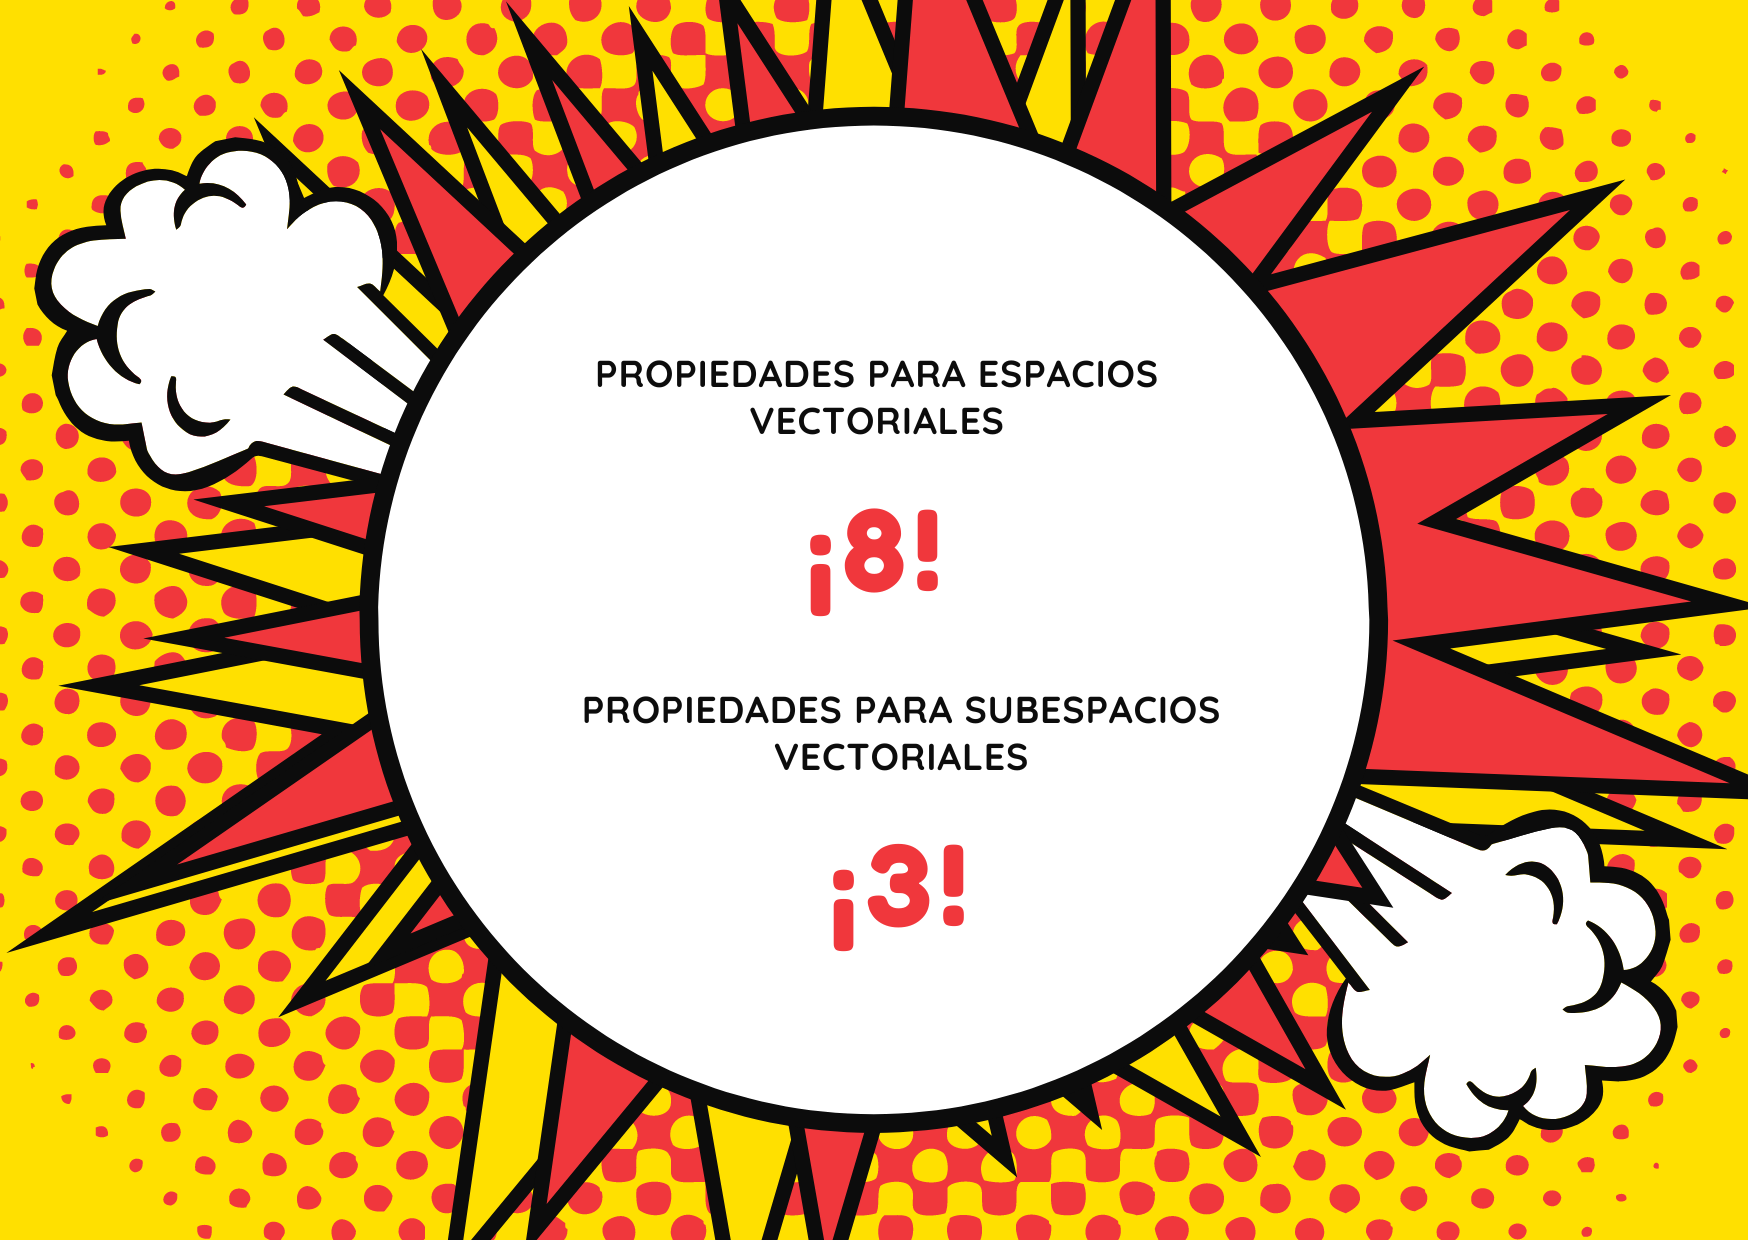
\includegraphics[width=0.60\textwidth]{Pictures/8.png}    
   % \label{TLfig10}
%\end{figure}




\section{Actividades propuestas}
%\subsection{}
\begin{answers}
Para realizar un cambio de coordenadas celestes a coordenadas horizontales\index{Cambio de coordenadas celestes}, es necesario hacer dos rotaciones:


\begin{figure}
    \centering
    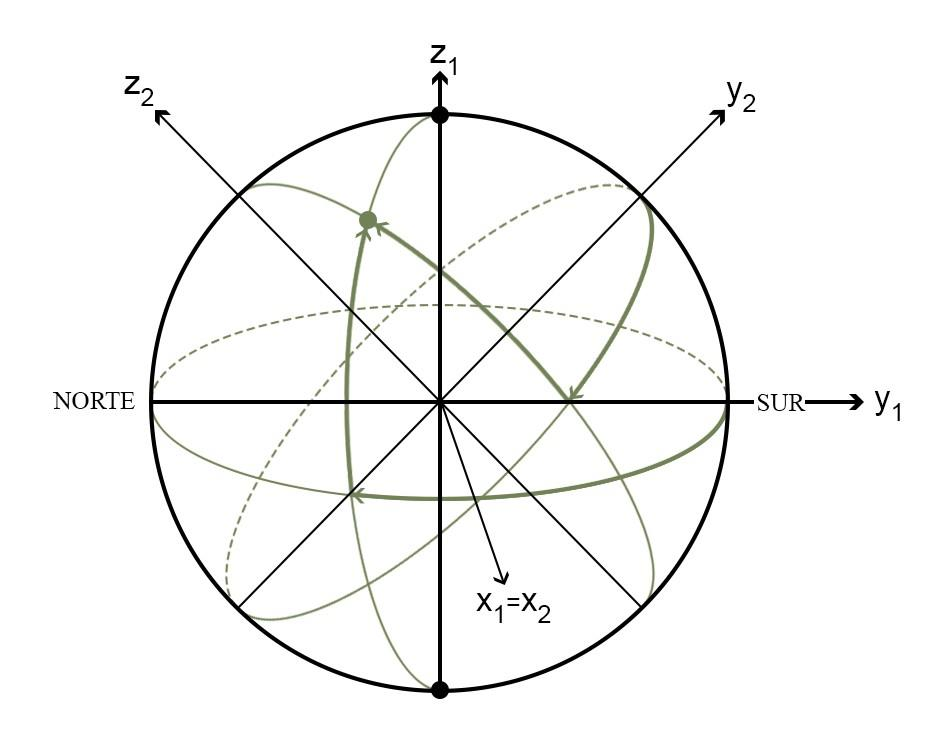
\includegraphics[width=0.7\textwidth]{Pictures/fig.42.jpg}
    \caption{Coordenadas $(x_1, y_1, z_1)$ y $(x_2, y_2, z_2)$ en el sistema cartesiano  horizontal y en el cartesiano  ecuatorial}
%horario respectivamente}
    \label{Esfera}
\end{figure}
%Figura nueva si se denotan con (x1, y1, z1) y (x2, y2, z2) las coordenadas de un astro en el
%sistema cartesiano tridimensional horizontal y en el cartesiano tridimensional ecuatorial
%horario respectivamente, teniendo en cuenta la definición de ambos sistemas, se
%obtienen por:

%\textcolor{red}{revisar fórmula no se aclara que son subindices  h, el y ec ? abajo si aclaro que son y como se escriben }

$$\vec{r}_{el}= R_z(TSL)*\vec{r}_{ec}$$

$$\vec{r}_{h}= R_y(90-\varphi)*\vec{r}_{el}$$

Esto se debe a que entre el sistema ecuatorial celeste y el ecuatorial local, el polo celeste (eje $z$) permanece  fijo para ambos, pero el origen desde donde medimos uno y otro sitema en el ecuador celeste, cambia en una cantidad TSL. Usaremos $TSL$ como tiempo siderio local, $TSL$= 18:31:31, Recuerde pasar de horas a grados para poder operar. Luego para realizar el cambio de coordenadas de celeste locales a horizontales, se mantiene en común el eje $y$, la línea este-oeste, y el ángulo en que se rotan el plano $x$, $z$ es $90-\varphi$. Para el problema actual usaremos la $\varphi$= $-$34º 50'  que corresponde a la ciudad de La Plata.

\bigskip

%\textcolor{red}{no entiendo la primera frase por qué entre, la reescribi pero tengo dudas. puse comas, revisar }

%\textcolor{red}{Esto se debe a que entre el sistema ecuatorial celeste y el sistema ecuatorial local, el polo celeste (eje $z$) permanece  fijo para ambos, pero el origen desde donde medimos uno y otro sistema en el ecuador celeste, cambia en una cantidad TSL. Usaremos $TSL$ como tiempo siderio local   $TSL= 18:31:31$, 
%Luego, para realizar el cambio de coordenadas de celestes locales a horizontales, se mantiene en común el eje $y$, la línea este-oeste, y el ángulo en que se rotan el plano $x$, $z$ es $90-\varphi$. Para el problema actual utilice  $\varphi= -34º 50'$,  que corresponde a la ciudad de La PLata. Creo haber agregado las comas ect..}

\bigskip

El vector de las coordenadas ecuatoriales celestes se escribe como:

\bigskip

$$\vec{r}_{ec}=\left(\begin{array}{c} cos(\delta)cos(\alpha)\\cos(\delta)sen(\alpha) \\ sen(\delta)
\end{array}
 \right)$$

 
\bigskip
\noindent
y el vector de las coordenadas horizontales:

$$\vec{r}_{h}=\left(\begin{array}{c} cos(h)cos(A)\\-cos(h)sen(A) \\ sen(h)
\end{array}
 \right)$$

 \bigskip
 
\noindent
donde $h=sen^{-1}(z)$ y $A=tan^{-1}(-y/x)$.

\bigskip
 
 Amplíe la Tabla \ref{cum} con las coordenadas horizontales para cada cúmulo.  Recuerde pasar de horas a grados para poder operar. Nota: No tenga en cuenta la precesión. \textcolor{blue}{Recomendación}: Realice un programa computacional para hacer los cálculos.

 
 \bigskip

%\end{document}

\begin{table}
%[!hbt]
\renewcommand{\tablename}{Tabla}
\centering
\begin{tabular}{L{0.15\textwidth} R{0.15\textwidth} R{0.15\textwidth}} 
%Specify column alignment with L{width}, C{width} and R{width} for fixed-%width columns, or the default latex l, c and r for flexible-width columns
		\toprule
		\textbf{Cúmulo} & \textbf{RA(J2000)} & \textbf{Dec(J2000)}\\%
		\midrule
NGC6192 &16:40:16.40 & $-$43:30:31.0\\
NGC6242 & 16:55:32.38& $-$39:28:02.0\\
NGC6322&17:18:25.13  & $-$42:56:03.3\\
NGC6704 &18:50:42.00 & $-$05:12:42.5\\
NGC6737 &19:02:16.30 & $-$18:32:56.5\\
Rup 102 & 12:13:32.95& $-$62:43:18.7\\
Rup 166 & 13:25:38.14& $-$63:27:54.6\\
SLS4565& 18:01:59.55&$-$23:41:06.3\\
Lynga 14& 16:55:03.40&$-$45:14:09.1\\
Trumpler 22& 14:31:03.33&$-$61:09:57.0\\
Trumpler 24& 16:56:11.14&$-$40:40:01.1\\
Dominici 11& 18:57:36.31&$-$10:23:39.9\\
Dominici 12& 18:51:24.93&$-$13:18:50.2\\
\bottomrule
\end{tabular}
\caption{Coordenadas celestes de 13 cúmulos abiertos.}
\label{cum} % Unique label used for referencing the table in-text
\end{table}

 


\end{answers}

\bigskip

 \bigskip

 

\subsection{Ejercicios}

%\subsubsection{Espacios Vectoriales. Subespacios. Suma de subespacios.}

 

%\newpage
\begin{exercise}
\item
Analice si los siguientes conjuntos son espacios vectoriales
sobre $\mathbb{R}$. 
%(asumiendo que $\oplus$ y $\ast$ son las operaciones naturales)

a) El conjunto  $S=\{(x,y) : y=2x+1\}
\subseteq \mathbb{R}^2$

b) El semiplano en $\mathbb{R}^2$,  $S=\{(x,y) : y\geq 0\}$, 

c) Los polinomios de grado menor o igual que 2, $P^{(2)}_{\mathbb{R}}[x]$.

\end{exercise}



\begin{exercise}
\item
Dé al menos $5$ ejemplos de espacios vectoriales y escriba según su opinión, 
qué utilidad podría tener saber que tienen estructura de espacio vectorial.
\end{exercise}
\begin{exercise}
\item 

De acuerdo con la definición; $S$ es un subespacio de un espacio vectorial $V$ sí 
y sólo sí, se cumplen las siguientes condiciones:

i) S contiene al vector $\vec{0}$ de $V$.

ii) Si $\vec{u}$ y $\vec{v}$ están en S, entonces $\vec{u}$  + $\vec{v}$ está en $S$.

iii) Si $\vec{u}$ está en $S$ y $\alpha$ es un escalar entonces, $\alpha\vec{u}$ está en $S$.

\noindent Compruebe si valen las siguientes afirmaciones:

\noindent a) $S=\{(x,y,z) : z=0\}$, es un subespacio de $\mathbb{R}^3$.

\noindent b) El conjunto de polinomios $P^{(2)}_{\mathbb{R}}[x]$, de grado menor o igual que $2$, es subespacio vectorial del espacio vectorial 
$P^{(n)}_{\mathbb{R}}[x]$ de todos los polinomios con coeficientes reales.


\end{exercise}

%\bigskip

\begin{exercise}
\item

Dados los subespacios de $\mathbb{R}^3$, $S$=$\{(x,y,z)\in \mathbb{R}^3: x=y=0\}$ y
$T=\{(x,y,z) \in \mathbb{R}^3: x+y+z=0\}$ calcule:
a) Una base y la dimensión de ambos subespacios.
b)  $S + T$ y $ S \cap T$, dando las bases de dichos subespacios.
c) ¿La suma $S + T$ es directa?
\end{exercise}

\begin{exercise}
\item

Encuentre en cada uno de los ejemplos siguientes la suma y la intersección del par de subespacios dados, y compruebe
que se verifica la ecuación:

\bigskip

    $dim(V_1)+dim(V_2) = dim(V_1+V_2) + dim(V_1 \cap V_2)$
    
\bigskip
		
		
a) Siendo el conmutador la diferencia entre $A.B - B.A$ con $A$ y $B$ matrices, y trabajando con que el conmutador sea necesariamente la matriz nula, encuentre los subespacios que se forman si $A$ es la matriz que se muestra en cada caso:

\bigskip

$A_1=\left(\begin{array}{cc} 2 & 1  \\ 0 & 2 
\end{array}
 \right), \qquad    A_2=\left(\begin{array}{cc} 2 & 0 \\ 1 & 2 
\end{array}
 \right)$\\
 
 \bigskip
 
b) Los subespacios formados por las bases $\{sen(t),cos(t)\}$ y $\{e^{it},e^{-it}\}$ considerados en el espacio real de las funciones complejas continuas en el intervalo $[0,1]$.
\end{exercise}

 
\begin{exercise} 
\item
 \begin{enumerate}
 
 \item 
 Demuestre que el conjunto de soluciones de la ecuación diferencial de primer orden homogénea, con coeficientes constantes:
 $y' + k y=0$ es un espacio vectorial de dimensión uno, siendo $\{e^{-kx}\}$ una base. A su vez el conjunto de soluciones de esta ecuación
 es un subespacio vectorial del espacio de las funciones derivables cuya dimensión es infinita.

\bigskip 
    
 
\item  Luego resuelva la ecuación diferencial homogénea de segundo orden:
 
 $y''- y' - 6y=0$, con las condiciones iniciales y(0)=3
 y y'(0)=-1.\\
 
  Dado que éste tipo de ecuaciones se resuelve usando la ecuación característica, que para éste caso sería:
 $\lambda^2-\lambda-6=0$.
 \begin{enumerate}
   
 \item Encuentre las raíces $\lambda_1$ y $\lambda_2$ y reemplazar en la función: $y(x)= C_1e^{\lambda_1 x}+C_2e^{\lambda_2 x}$.
 
 \item Escriba la base del conjunto solución, y especifique que dimensión tiene. 
 \item Halle la solución particular definiendo los coeficientes $C_1$ y $C_2$, con ayuda de las condiciones iniciales.
 \end{enumerate}
 \item Averigue que pasaría si las soluciones de la ecuación característica de una ecuación diferencial homogénea fueran raíces dobles. Escriba su base.
 
\item Cite al menos un ejemplo de física donde se necesita usar ecuaciones diferenciales.
\end{enumerate}
\end{exercise}

\begin{exercise}
\item

¿Son los vectores  $\vec{u}=(4,-2,5)$ y $\vec{v}=(1,-1,-1)$ de $\mathbb{R}^3$ combinación lineal
de $\vec{x_1}=(1,-1,2)$ y $\vec{x_2}=(2,0,1)$? Interprete geométricamente y conecte con los subespacios de 
$\mathbb{R}^3$.
\end{exercise}

\begin{exercise}
\item

Los primeros cuatro polinomios de Laguerre son  $\{1, 1-x, 2-4x+x^2, 6-18x + 9x^2 - x^3\}$. Demuestre que estos polinomios forman una base de $P^{(3)}_{\mathbb{R}}[x]$.
\end{exercise}

\begin{exercise}
\item

Compruebe que $B=\{1,x,x^2\}$ es una base del espacio vectorial $P^{(2)}_{\mathbb{R}}[x]$. En consecuencia dim$(P^{(2)}_{\mathbb{R}}[x])$= 3.
¿Es correcta la afirmación dim$(P^{(n)}_{\mathbb{R}}[x])$= n+1?
 \end{exercise}
\begin{exercise}
\item

Sea la matriz, 


$$A=\left(\begin{array}{ccc}x & a & b \\ a & x & b\\ a & b & x 
\end{array}
 \right)$$

 \bigskip
\noindent 
Encuentre los valores de $x$ para los que el $Det (A)= 0$. Lo cual es equivalente a decir que columnas o filas son linealmente dependientes.
¿Cuáles son las dimensiones posibles del espacio generado por las filas?

\end{exercise}





%\subsubsection{Bases. Coordenadas de  un vector en una base. Cambio de base.}


 
\begin{exercise}
\item

Encuentre las coordenadas del vector  $\vec{x}=(1,3,-2)$ con respecto a la base B=$\{\vec{b_1}, \vec{b_2}, \vec{b_3}\}$
donde $\vec{b_1}=(1,0,0)$, $\vec{b_2}=(1,1,0)$, $\vec{b_3}=(1,1,1)$.

\bigskip

\end{exercise}

\begin{exercise}
\item
 Calcule las coordenadas del vector $\vec{w}$ relativas a la base
$B=\{ \vec{u}_1,\vec{u}_2\}$.

a) $\vec{u}_1=(1,0)$, $\vec{u}_2=(0,1)$; $\vec{w}=(3,7)$

b) $\vec{u}_1=(2,-4)$, $\vec{u}_2=(3,8)$; $\vec{w}=(1,1)$

c) $\vec{u}_1=(1,1)$, $\vec{u}_2=(0,2)$; $\vec{w}=(a,b)$\\

\end{exercise}

\begin{exercise}
\item
Encuentre las coordenadas del vector $\vec{v}$ relativas a la base $B=\{
\vec{v}_1,\vec{v}_2,\vec{v}_3\}$.

 $\vec{v}_1=(1,0,0)$, $\vec{v}_2=(2,2,0)$, $\vec{v}_3=(3,3,3)$; $\vec{v}=(2,-1,3)$.\\
\end{exercise}

\begin{exercise}
\item

Calcule las coordenadas del vector $p \in P^{(2)}_{\mathbb{R}}[x]$ relativas a la base $B=\{
p_1(x),p_2(x),p_3(x)\}$.



$p_1(x)=1+x$, $p_2(x)=1+x^2$, $p_3(x)=x+x^2$; $p(x)=4-3x+x^2$\\
\end{exercise}
\begin{exercise}
\item
En $\mathbb{R}^{2\times2}$, encuentre las coordenadas de la matriz
$A=\left(\begin{array}{cc}2 & 0  \\-1 & 3
\end{array}
 \right)$ relativas a la base


\[ B= \left\{
 \left(\begin{array}{cc}-1 & 1  \\0 & 0
\end{array}
 \right),\left(\begin{array}{cc}1 & 1  \\0 & 0
\end{array}
 \right),\left(\begin{array}{cc}0 & 0  \\1 & 0
\end{array}
 \right),\left(\begin{array}{cc}0 & 0  \\0 & 1
\end{array}
 \right)
 \right \}
 \]\\
\end{exercise}
\begin{exercise}
\item 


Considere las bases $B=\{ \vec{u}_1,\vec{u}_2\}$  y $B^\prime=\{ \vec{v}_1,\vec{v}_2\}$ para
$ \mathbb{R}^2$, donde  $\vec{u}_1=(1,0)$, $\vec{u}_2=(0,1)$, $\vec{v}_1=(2,1)$,
$\vec{v}_2=(-3,4)$.

a) Halle la matriz de cambio de base de $B$ a $B^\prime$, $P_{B^\prime,B}$.

b) Utilice la matriz anterior para obtener las coordenadas en la base
$B^\prime$ de $\vec{w}=(3, -5)_{B}$.

c) Verifique lo obtenido en b) haciéndolo directamente.

d) Calcule la matriz de transición $P_{B,B^\prime}$ y verifique que
$P_{B,B^\prime}= P^{-1}_{B^\prime,B}$.
\end{exercise}

\begin{exercise}
\item

Considere las bases $B=\{ \vec{u}_1,\vec{u}_2, \vec{u}_3\}$  y $B^\prime=\{ \vec{v}_1,\vec{v}_2,
\vec{v}_3\}$ para $ \mathbb{R}^3$, donde  $\vec{u}_1=(-3,0,-3)$,
$\vec{u}_2=(-3,2,1)$, $ \vec{u}_3=(1,6,-1)$, $ \vec{v}_1=(-6,-6,0)$, $\vec{v}_2=(-2,-6,4)$ y
$\vec{v}_3=(-2,-3,7)$.\\

a) Halle la matriz de cambio de base de $B$ a $B^\prime$.


b) Utilice la matriz anterior para obtener las coordenadas en la base
$B^\prime$ de $\vec{w}=(-5, 8, -5)_{B}$.
\end{exercise}



\begin{exercise}
\item

Considere las bases $B=\{ p_1(x),p_2(x)\}$  y $B^\prime=\{ q_1(x),q_2(x)\}$ para
$P^{(1)}_{\mathbb{R}}[x]$, donde  $p_1(x)=6+3x$, $p_2(x)=10+2x$, $q_1(x)=2$, $q_2(x)=3+2x$.

a) Halle la matriz de transición de $B$ a $B^\prime$.

b) Utilice la matriz anterior para obtener las coordenadas de $p(x)=-4+x$
en la base $B^\prime$.\\
\end{exercise}
%\vspace{0.15cm}



\begin{exercise}
\item

Si se quiere obtener un sistema de coordenadas rectangulares
$x'y'$ haciendo girar un sistema de coordenadas rectangulares $xy$ hasta
describir un ángulo de $\theta= \frac {3 }{4} \pi$.

a) Halle las coordenadas $x^\prime y^\prime$ del punto cuyas coordenadas $xy$
son $(-2,6)$.

b) Calcule las coordenadas $xy$ del punto cuyas coordenadas $x^\prime y^\prime$
son $(5,2)$.

%\vspace{0.15cm}
\end{exercise}

\begin{exercise}
\item

Si se quiere obtener un sistema de coordenadas rectangulares
$x^\prime y^\prime z^\prime$ haciendo girar un sistema de coordenadas rectangulares $xyz$ en sentido
contrario a las agujas del reloj alrededor del eje $z$, cuando se
observa hacia abajo a lo largo del eje $z$ hasta describir un
ángulo de $\theta= \frac {\pi}{4}$.

a) Halle las coordenadas $x^\prime y^\prime z^\prime$ del punto cuyas coordenadas
$xyz$ son $(-1,2,5)$.

b) Calcule las coordenadas $xyz$ del punto cuyas coordenadas
$x^\prime y^\prime z^\prime$ son $(1,6,-3)$.

\end{exercise}



 %\subsection{Ejercicios teóricos}\\
 
\begin{exercise}
\item

Sea $V$ un espacio vectorial de dimensión $n$. Demuestre que todo conjunto linealmente independiente de $n$ elementos es una base de $V$.
\end{exercise}

\begin{exercise}
\item

Sean $p_0(x), p_1(x),.., p_n(x)$ polinomios cualesquiera de $P^{(n)}_{\mathbb{R}}[x]$ de grado $0,1,  \cdots,n$ respectivamente: demuestre que 
$\{p_0(x), p_1(x),..,p_n(x)\}$ es una base de $P^{(n)}_{\mathbb{R}}[x]$. ¿Podría encontrar alguna relación entre este teorema y el teorema del resto?
¿Y con la fórmula de Taylor?
\end{exercise}
\begin{exercise}
\item

En el supuesto que V=$V_1\oplus V_2$ donde $V_1$ y $V_2$ son dos subespacios de V de dimensiones n y m respectivamente y sean $B_1=\{\vec{u}_1,\vec{u}_2,\cdots,\vec{u}_n\}$ y $B_2=\{\vec{v}_1,\vec{v}_2,\cdots,\vec{v}_n\}$ sus bases, compruebe que $B=B_1 \cup B_2$ es una base de $V_1\oplus V_2$.
\end{exercise}

\bigskip


\bigskip

\begin{exercise}
\item
Sea $A=LU$, donde $L$ es una matriz triangular inferior invertible y $U$ es triangular superior. Explique por qué la primera columna de $A$ es un múltiplo de la primera columna de $L$. ¿Cómo se relaciona la segunda columna de $A$ con las columnas de $L$?\\
\end{exercise}



\begin{exercise}
\item
Sea $\{\vec{e_1},\vec{e_2},\cdots,\vec{e_n}\}$ la base canónica de $\mathbb{R}^n$, y sean $\vec{u_1}=\vec{e_2}- \vec{e_1}$, $\vec{u_2}=\vec{e_3}- \vec{e_2}, \cdots,  \vec{u_n}=\vec{e_{n}}- \vec{e_{n-1}}$. 
Demuestre que  $\{\vec{u_1},\vec{u_2},\cdots,\vec{u_n}\}$ es una base de $\mathbb{R}^n$.
Exprese el vector $ \vec{v} = \vec{e_1}+ \vec{e_2}+\cdots+\vec{e_n}$  como una combinación lineal de los vectores $\vec{u_1},\vec{u_2},\cdots,\vec{u_n}$.\\


\end{exercise}


%\newpage

\bigskip

 \subsection{Autoevaluación}
 \label{Auto1}
 

\subsubsection{Verdadero o Falso.}


 \bigskip

\begin{enumerate}

\item

Si una matriz tiene dos filas iguales, su determinate vale $0$.

\item

Si F= $F_1 \oplus F_2 \oplus .. \oplus F_p$ entonces dim F $ \neq $ dim $F_1$ + dim $F_1$ + .. + dim $F_p$.

\item

Si $P_{B,A}$ es invertible, entonces $P^{-1}_{B,A}$=$P_{B,A}$.

\item

Siendo $A$,$ B$ y $C$  bases de un espacio vectorial,  se cumple que $P_{C,B}.P_{B,A}$=$P_{C,A}$. 

\item

 Sea S un conjunto de un espacio vectorial V de dimensión n y además S contiene menos de n vectores, entonces S no puede generar V.

\item

Un plano en $\mathbb{R}^3$ es un subespacio de dimensión $2$ de $\mathbb{R}^3$.


\item

Si un conjunto $\{\vec{v_1},\vec{v_2},\cdots,\vec{v_p}\}$ genera un espacio vectorial V de dimensión finita y si T es un conjunto de más de p vectores en V, entonces T es linealmente dependiente.

\item

La suma del subespacio de  las matrices simétricas de $\mathbb{R}^{n \times n}$  con las matrices antisimétricas de $\mathbb{R}^{n \times n}$ es directa generando el espacio vectorial de las matrices de $\mathbb{R}^{n \times n}$.

\item

La suma del subespacio de las  funciones pares con el subespacio de las funciones impares no es directa.

\end{enumerate}









%--------------------------------------------------------------
%	More sections?
%----------------------------------------------------------------------------

\chapterimage{Pictures/blue_space(1).jpg}



%Y ese conjunto junto con el producto interno forman en por sí mismo un espacio vectorial. Hemos trabajando con varios durante las prácticas:
%Los polinomios, dado un x el resultado es un escalar, también la traza y el determinante, incluso integrales de productos de funciones o series como %en el caso de Fourier, ahora bien todos estos funcionales son justamente los elementos del espacio dual.
%En física si un vector representa la velocidad de una partícula su funcional será el momento angular. Por lo que resultaría interesante saber cómo %encontrar éstos funcionales asociados.\\

%Si estamos trabajando en una base ortonormal es fácil ver que, por ser paralelos, el producto entre el vector y su funcional será necesariamente 1, %mientras que para los demás vectores que son perpendiculares al primero el producto debe dar 0. Con esta información construimos un sistema de %ecuaciones y encontramos los coeficientes necesarios. Aquellos funcionales que anulan a ese vector están en el espacio anulador del vector. Pero el %espacio anulador es más interesante cuando se aplica a conjunto de vectores.\\

%Otro ejemplo: En el espacio Euclídeo un vector puede representarse como una flecha, entonces dado un vector, el funcional asociado a ese vector y que %vive en el espacio dual será el que genera todos los vectores paralelos a ese vector. Uno puede saber el vector o el funcional y tendrá información %sobre ambos.\\

%Para decirlo de una forma más simple, supóngase que un vector es el cuadro de la Monalisa, el cuadro puede dividirse entre el fondo (el paisaje) y la %forma (el rostro de Monalisa). Como puede verse fácilmente el fondo determina la forma y viceversa por eso la denominación dual. Así mismo se llama %doble dual, al dual del dual que no es otro que el espacio vectorial V, pero nos sirve porque es la forma de pasar del dual al espacio V. \\ 



%Una transformación (o función o mapeo) $T:\mathbb{R}^n \rightarrow \mathbb{R}^m$ asigna a cada vector $\vec{x}$ en $\mathbb{R}^n$ %%%%5(dominio) un vector $T(\vec{x})$ en $\mathbb{R}^m$ (codominio). A su vez el mapeo dado por T del dominio al codominio se asocia a una %multiplicación matricial $T(\vec{x})=A\vec{x}$ donde A es la matriz de la transformación. Esta matriz genera dos espacios de particular %interés para el álgebra, el subespacio anulador o núcleo de T y el subespacio de la columnas de A o imagen de T. Un resultado muy %importante es que la suma de las dimensiones de estos subespacios siempre será igual a la dimensión del dominio de T.


\chapter{Transformaciones Lineales}

En este capítulo nos interesamos por aquellas aplicaciones entre espacios vectoriales que preservan las operaciones de suma y producto por escalares. Son las aplicaciones o transformaciones lineales. Son las funciones con las que se trabaja en Álgebra Lineal y tienen uma amplia variedad de aplicaciones.  Se verá que, en el caso de dimensión finita,  es posible  asociarles una matriz. Se estudian los espacios asociados; el espacio nulo y el espacio que generan las columnas de la matriz. Un resultado útil e importante es que las sumas de las dimensiones de esos subespacios da la dimensión del espacio de partida. Mostramos la interpretación geométrica tanto de las aplicaciones lineales en el plano como en el espacio. Se presentan una gran variedad de ejemplos.\\
Se  estudia, además, el espacio dual de un espacio vectorial. Es el conjunto de todas las transformaciones lineales entre un espacio vectorial y el cuerpo de los escalares, conocidas como funcionales lineales. 
%Las transformaciones (o aplicaciones) lineales son las funciones con las que se trabaja en Algebra Lineal. Son funciones que van de un %espacio vectorial a otro y tienen una gran variedad de aplicaciones.

\section{Definición de transformación lineal. Ejemplos.}

\bigskip

\begin{definition}\label{TL}\index{Transformación lineal}


Sean $V$ y $W$ dos espacios vectoriales, una \textit{transformación lineal} $T$ de $V$ en $W$ es una aplicación $T: V \rightarrow W$ tal que: 


\bigskip

\begin{enumerate}

\item $T(\vec{v}+\vec{w})=T(\vec{v})+T(\vec{w})$ para todo  $\vec{v}$, $\vec{w}$ $\in V$.

\item $T(a ~\vec{v})=a~T(\vec{v})$ para todo $a\in K$ y todo $\vec{v}$ $\in V$.
  

\end{enumerate}

\end{definition}

\bigskip

\bigskip

Entre las transformaciones lineales más utilizadas están las proyecciones. En la Figura \ref{figproyxy} se muestra la proyección ortogonal  de un vector $\vec{v}=(x,y,z)$ sobre el plano $xy$. \index{Proyección ortogonal}

\bigskip

Se tiene $T: \mathbb{R}^3 \rightarrow \mathbb{R}^3$, donde $   T((x,y,z))=(x,y,0)$.
Es una transformación lineal ya que se cumplen para $ \forall ~ \vec{v}=(x,y,z)$, $\vec{w}=(x^{\prime},y^{\prime},z^{\prime})$ y  $ \forall ~a\in K$:



\bigskip

\begin{enumerate}

\item $T(\vec{v}+\vec{w})=T((x+x^{\prime},y+y^{\prime},z+z^{\prime}))= (x+x^{\prime},y+y^{\prime},0) =(x,y,0)+ (x^{\prime},y^{\prime},0)= T(\vec{v})+ T(\vec{w})$.

\bigskip

\item $T(a ~\vec{v})= T( a  (x,y,z)) = T((ax,ay,az)) = (ax,ay,0)=a(x,y,0)=   a~T(\vec{v})$.
  

\end{enumerate}



\bigskip


\begin{figure}[!htbp]
\label{figproyxy}
    \centering
    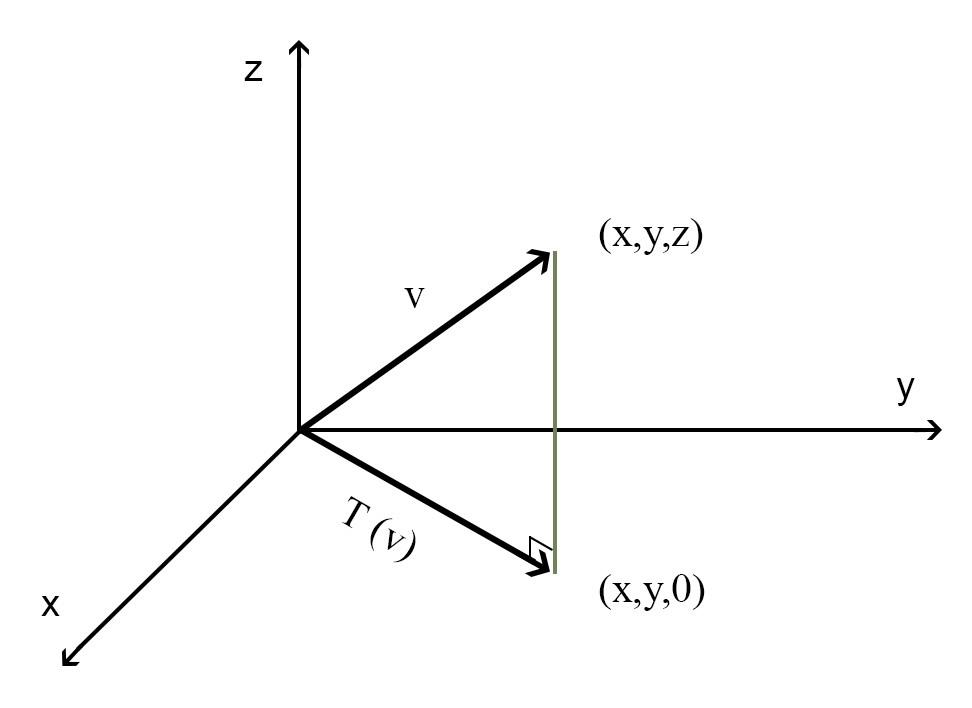
\includegraphics[width=0.60\textwidth]{Pictures/TLfig10.jpg}
    \caption{Proyección ortogonal de un vector $\vec{v}$ sobre el plano $xy$. }
    %\label{TLfig10}
\end{figure}

\begin{remark}
\begin{itemize}
\item En una transformación lineal $V$ y $W$ deben ser espacios vectoriales sobre el mismo cuerpo $K$.

\item Las aplicaciones  $O: V \rightarrow W$, $O(\vec{u})= \vec{0}_W$ para todo $\vec{u} \in V$ y 
$I_d: V \rightarrow V$, $I_d(\vec{u})= \vec{u}$ son  transformaciones lineales.

\item La traza de una matriz, \index{Traza de una matriz}

$Tr: K^{n \times n } \rightarrow K $ dada por $Tr(A)=\sum_{i=1}^n a_{ii}$, es una transformación lineal.



\item $T: \mathbb{R} \rightarrow \mathbb{R}$ dada por $T(x)=x^2$ es un ejemplo de  transformación \textit{no lineal}.
Se tiene que $T(x+y) \neq T(x) + T(y)$, ya que $T(x+y) = (x+y)^2= x^2 + y^2+2xy$,   mientras que $T(x)+T(y) = x^2 + y^2$.
\item
Otro ejemplo de transformación no lineal es el determinante de una matriz, ya que, en general  $Det(A+B) \neq Det(A)+Det(B)$.
\end{itemize}
%\hfill$\blacktriangle$
\end{remark}


\bigskip

\begin{example}
Dado un número real $a$, la aplicación que asocia a cada polinomio $p$ del conjunto  $P_\mathbb{R}\left[t\right]$ su valor en $x=a$, $p(a)$, es una transformación lineal. Está definida mediante las siguientes expresiones: 

$$T: P_\mathbb{R}\left[t\right] \rightarrow \mathbb{R}$$ 

$$T(p(t))=p(a)$$


El hecho que $T$ es una transformación lineal se deduce de las igualdades $T(p+q)=T(p) + T  (q)$ y $T(cp)=cT(p)$ que se prueban a continuación:

$$T(p+q)(t)=(p+q)(a)=p(a)+q(a)=T(p)(t)+T(q)(t)$$


\noindent
y
$$T(cp)(t)=(cp)(a)=c(p(a))=cT(p)(t)$$
\noindent
para todo número real $c$.
\end{example}




\bigskip

\index{Imagen de una transformación lineal}
Aplicando repetidas veces las propiedades $1$ y $2$  de la definición de transformación lineal entre espacios vectoriales $V$ y $W$ se puede ver que la imagen de una combinación lineal de vectores  del espacio vectorial inicial $V$ es una combinación lineal de vectores del espacio vectorial final $W$, es decir 

$$T(\sum_{j=1}^{n}c_j\vec{v}_j)=\sum_{j=1}^{n}c_jT(\vec{v}_j)$$

\bigskip
\noindent
donde $c_j  \in K$ y $\vec{v}_j  \in V$  para todo $j=1,2, \cdots, n$.


\bigskip


\bigskip

\bigskip

Otras propiedades de las transformaciones lineales que se deducen de la definición  se enuncian en las proposiciones a continuación.

\bigskip

\bigskip



\begin{theorem}
\label{Prop31}

Sea $T$ una aplicación lineal entre dos espacios vectoriales $V$ y $W$. Se tienen los siguientes resultados:

\begin{enumerate}

\item La imagen del elemento neutro de $V$ mediante $T$ es el neutro de $W$, es decir, $T(\vec{0}_V)= \vec{0}_W$


\item La imagen mediante T del opuesto de un elemento  $\vec{v}\in V$ es el opuesto de $T(\vec{v})$, es decir,  $T(-\vec{v})=-T(\vec{v})$

\end{enumerate}

\begin{proof}

\begin{enumerate}

\item  $T(\vec{0}_V)= T(\vec{0}_V +\vec{0}_V )= T(\vec{0}_V) + T(\vec{0}_V)$

%\noindent
Restando $T(\vec{0}_V)$ en ambos miembros de la igualdad, se tiene 

\bigskip

$T(\vec{0}_V)- T(\vec{0}_V)= T(\vec{0}_V)$
\noindent
de donde, $\vec{0}_W  = T(\vec{0}_V) $.

\bigskip

\item     $T(-\vec{v})= T((-1)\vec{v})= (-1)T(\vec{v})=  -T(\vec{v})$, $ \forall ~ \vec{v}\in V$.

\end{enumerate}

\end{proof}

\end{theorem}

\bigskip

\bigskip

\begin{theorem}
\label{Prop32}


Sea $T: V \rightarrow W$ una transformación lineal entre espacios vectoriales. La imagen mediante $T$ de cualquier subespacio vectorial $V_1$ de $V$, $W_1=T(V_1)$ es un subespacio vectorial de $W$.

\begin{proof}

\begin{itemize}

\item
$0_W  \in T(V_1)$, ya que $T(0_V)= 0_W$.

\item
Sean $\vec{w}_1$ y $\vec{w}_2$ $\in T(V_1)$. Existen  $ \vec{v}_1, \vec{v}_2  \in V_1$ tales que $T(\vec{v}_1)=\vec{w}_1$ y $T(\vec{v}_2)=\vec{w}_2$. Para ver que $\vec{w}_1 + \vec{w}_2$ $\in T(V_1)$ basta ver que,  por ser $V_1$ subespacio, $\vec{v}_1+ \vec{v}_2  \in V_1$  y $T(\vec{v}_1+ \vec{v}_2)=  T(\vec{v}_1)+T(\vec{v}_2)=\vec{w}_1 + \vec{w}_2$.

\item
Y también $\alpha\vec{w}_1$ $\in T(V_1)$, ya que $\alpha\vec{v}_1  \in V_1$, por ser $V_1$ subespacio, y  $T(\alpha   \vec{v}_1)=  \alpha T(\vec{v}_1)=\alpha \vec{w}_1$ .


\end{itemize}
\end{proof}
\end{theorem}


\bigskip

\bigskip


\begin{theorem}
\label{Prop33}




Sea $T: V \rightarrow W$ una transformación lineal entre espacios vectoriales. Si $U$ es un subespacio de $W$, entonces 
$T^{-1}(U)=\left\{\vec{v} /\vec{v} \in V, T(\vec{v})~ \in U \right\}$ es un subespacio de $V$.

\begin{proof}
\begin{itemize}

\item
$0_V  \in T^{-1}(U)$, ya que $T^{-1}(0_W)= 0_V$.


\item

Sean $\vec{v}_1$ y $\vec{v}_2$ $\in T^{-1}(U)$. Existen $ \quad \vec{u}_1$ y $\vec{u}_2$  $\in W$ tales que $T(\vec{v}_1)=\vec{u}_1$  y $T(\vec{v}_2)=\vec{u}_2$. Como $T(\vec{v}_1+\vec{v}_2)= T(\vec{v}_1)+T(\vec{v}_2)$ $\in U$, 
$\vec{v}_1+\vec{v}_2$ $\in T^{-1}(U)$.
\item

De  la misma forma,  si $ \vec{v}_1$ $\in T^{-1}(U)$, $\alpha \vec{v}_1$ $\in T^{-1}(U)$ pues $T( \alpha \vec{v}_1)=  \alpha T(\vec{v}_1)= \alpha  \vec{u}_1$. 

\end{itemize}

\end{proof}

\end{theorem}

\bigskip



\bigskip


\begin{theorem}
\label{Prop34}

La imagen mediante una transformación lineal de un subespacio vectorial de dimensión $k$ es un subespacio vectorial de dimensión no superior a $k$.

\begin{proof}
Por la Proposición  \ref{Prop32}, si el subespacio $V_1$ de $V$ tiene $\left\{\vec{v}_1,\vec{v}_2,\cdots, \vec{v}_k\right\}$ como base, todo elemento $w$ de la imagen de $W_1=T(V_1)$ puede escribirse como combinación lineal de los vectores $T(\vec{v}_1),T(\vec{v}_2),\cdots, T(\vec{v}_k)$.  Esto es cierto ya que tomando $\vec{v}\in V_1$  tal que $T(\vec{v})=\vec{w}$ se tiene que 

$$\vec{w}=T(\vec{v})=T(\sum_{j=1}^{k}c_j\vec{v}_j)=\sum_{j=1}^{k}c_jT(\vec{v}_j).$$


Por lo tanto,  $W_1$ coincide con el subespacio generado por los vectores $T(\vec{v}_1),T(\vec{v}_2),\cdots, T(\vec{v}_k)$,
$$  \langle T(\vec{v}_1),T(\vec{v}_2),\cdots, T(\vec{v}_k)   \rangle$$

Es decir $W_1=\bold{L}(T(\vec{v}_1),T(\vec{v}_2),\cdots, T(\vec{v}_k))$.  $T$ preserva las combina-\ ciones lineales.

En consecuencia, la dimensión de $W_1$ no puede superar $k$.


\end{proof}

%\begin{proof}

%Si $V_1$ tiene como base a ${\vec{v}_1,\vec{v}_2, \cdots \vec{v}_k}$, la imagen se puede escribir como combinación lineal de los vectores 
%$T(\vec{v}_1), T(\vec{v}_2), \cdots, T(\vec{v}_k)$, $W= L( T(\vec{v}_1), T(\vec{v}_2), \cdots, T(\vec{v}_k))$ y por lo tanto la dimensión %no puede ser superior a $k$.

%\end{proof}




\end{theorem}
%\noindent

\bigskip

\bigskip

Demostraremos con el teorema que sigue  que una transformación queda determinada cuando se conocen las imágenes de los elementos de una base del espacio vectorial inicial.

\bigskip

\bigskip


\begin{theorem}
\label{TEO1}


Sea $B= \left\{\vec{e}_1,\vec{e}_2,\cdots, \vec{e}_n\right\}$ una base de un espacio vectorial $V$  y sean $\vec{w}_1,\vec{w}_2,\cdots, \vec{w}_n$ $n$ vectores cualesquiera de otro espacio vectorial $W$. En estas condiciones, existe una única transformación lineal $T$ de $V$ en $W$ tal que 

$$T(\vec{e}_j)=\vec{w}_j, ~~
j=1,2, \cdots, n$$

\begin{proof}
\begin{itemize}
\item
Existencia.
Dado $\vec{v} \in V$,  $\vec{v}= \sum_{j=1}^{n} \alpha_j \vec{e}_j  $ con $\alpha_j \in K$.
Se define $T(\vec{v})= \sum_{j=1}^{n} \alpha_j \vec{w}_j $.  
\item
T es lineal


Sean $\Vec{v}$ y $\Vec{v}^{\prime}$  tales que $\vec{v}= \sum_{j=1}^{n} \alpha_j \vec{e}_j  $ y $\vec{v}^{\prime}= \sum_{j=1}^{n} \alpha_j^{\prime} \vec{e}_j  $. Entonces,
$$\vec{v}  +\vec{v}^{\prime} =  \sum_{j=1}^{n} \alpha_j \vec{e}_j + \sum_{j=1}^{n} \alpha_j^{\prime} \vec{e}_j =\sum_{j=1}^{n}( \alpha_j + \alpha_j^{\prime}) \vec{e}_j  $$
y 
$$   T(\vec{v} + \Vec{v}^{\prime}  )= \sum_{j=1}^{n} ( \alpha_j + \alpha_j^{\prime}) \vec{w}_j = \sum_{j=1}^{n} \alpha_j  \vec{w}_j + \sum_{j=1}^{n} \alpha_j^{\prime} \vec{w}_j =T(\vec{v}) + T(\Vec{v}^{\prime} ) $$

De la misma forma, 

$$   T(c\vec{v} )= \sum_{j=1}^{n} (c \alpha_j ) \vec{w}_j = c \sum_{j=1}^{n} \alpha_j  \vec{w}_j  = cT(\vec{v}) $$
\item
$T$ es única

Si $T^{\prime}$ cumple  $T^{\prime}(\vec{e}_j)=\vec{w}_j$ y $\vec{v}= \sum_{j=1}^{n} \alpha_j \vec{e}_j  $,  se tiene que 


$$T^{\prime}(\vec{v})= \sum_{j=1}^{n} \alpha_j T^{\prime}(\vec{e}_j)= \sum_{j=1}^{n} \alpha_j T(\vec{e}_j)=T(\vec{v}).$$

\bigskip


Luego $T( \vec{v})=T^{\prime}(\vec{v}) $, $\forall  \vec{v} \in V $, de donde $T=T^{\prime} $.

\end{itemize}
\end{proof}
\end{theorem}

\bigskip

\bigskip

Se presentan a continuación  ejemplos de  transformaciones lineales  conocidas  como  la derivada, la integral definida (entre espacios vectoriales de funciones) y la multiplicación de una matriz por un vector. Se deja  al lector  la verificación de  que son transformaciones lineales.

\bigskip

\bigskip


\begin{example}
\label{ejderi}
$D: P_{\mathbb{R}}^{(n)}[x] \rightarrow  P_{\mathbb{R}}^{(n-1)} [x] $  (derivada)
$$D(a_01+a_1x+a_2x^{2} + \cdots +a_nx^{n}) = a_1+ 2 a_2x + \cdots +n a_nx^{n-1}     $$
\end{example}

\begin{example}

$J: ~C([0,1])\rightarrow  \mathbb{R}  $     (integral definida)

$$J(f)=\int_0^1 f(x)dx $$

\end{example}

\bigskip
  

\begin{example}

Dada la matriz, 
$$A=\left(\begin{array}{ccc} i & 1 &  0\\
1 &  i  &  0
\end{array}\right)$$

\noindent
es posible definir la transformación que multiplica la  matriz por un vector $ \vec{v}=(z_1,z_2,z_3)  \in \mathbb{C}^2$, es decir,   $A:\mathbb{C}^3 \rightarrow \mathbb{C}^2 $, está  dada por $A ((z_1,z_2,z_3))= A (z_1,z_2,z_3)^t$.

Es una transformación lineal, ya que se cumple
$$ A (\vec{v} + \vec{v}^{\prime})= A \vec{v} + A\vec{v}^{\prime} $$

y  $$ A (c \vec{v})= c  A \vec{v} $$

\end{example}



\begin{remark}
\label{AyT}
\begin{itemize}
    \item 
Dada una matriz $A \in K^{m \times n } $, la transformación  $A:K^n \rightarrow K^m $, dada por 
$$A ((z_1,z_2, \cdots, z_n)) = A (z_1,z_2, \cdots, z_n)^T,$$ es la transformación lineal asociada con la matriz $A$.
\item
Se verá  que, recíprocamente, dada una transformación lineal es posible hallar la matriz que la representa.
\end{itemize}
%\hfill$\blacktriangle$
\end{remark}

\bigskip

\section{Matriz  de una transformación  lineal.}\index{Matriz de una transformación lineal}
\label{MatrizdeunaTL}


Sean $V$ y $W$ dos espacios vectoriales sobre el mismo cuerpo $K$. Sea $B= \left\{\vec{e}_1,\vec{e}_2,\cdots, \vec{e}_n\right\}$ una base  de $V$ y $\bar{B}= \left\{\vec{f}_1,\vec{f}_2,\cdots, \vec{f}_m\right\}$ una base  de $W$. El elemento $T(\vec{e}_1)$ es un vector de $W$, y por lo tanto puede escribirse como combinación lineal de los vectores de  la base $\bar{B}$:

\bigskip

$$T(\vec{e}_1)=a_{11}\vec{f}_1+a_{21}\vec{f}_2+\cdots + a_{m1}\vec{f}_m$$ 

Análogamente, 

$$T(\vec{e}_2)=a_{12}\vec{f}_1+a_{22}\vec{f}_2+\cdots + a_{m2}\vec{f}_m$$ 
$$  \cdots                \cdots                  \cdots $$
$$T(\vec{e}_n)=a_{1n}\vec{f}_1+a_{2n}\vec{f}_2+\cdots + a_{mn}\vec{f}_m.$$ 

\bigskip



Estas igualdades se escriben de la forma

\bigskip
\begin{equation}
\label{Tej0}
T(\vec{e}_j)=\sum_{i=1}^{m}a_{ij}\vec{f}_i,~~ j=1,2 \cdots,n
\end{equation}

\bigskip
O en forma más abreviada, usando notación indicial, es decir sumando sobre el índice repetido $i$ de $1$ a $m$,


\bigskip

$T(\vec{e}_j)=a_{ij}\vec{f}_i,~~ j=1,2 \cdots,n$

\bigskip

En estas condiciones diremos que 

\bigskip


\bigskip

$$T=\left(\begin{array}{cccc}a_{11} ~&a_{12}  ~& a_{13} ~\cdots &a_{1n}~\\
a_{21} ~&a_{22}  ~& a_{23} ~\cdots &a_{2n}~\\ 
   ~ ~ ~ ~ ~  \cdots \cdots    
\\ a_{m1} ~&a_{n2}  ~& a_{m3} ~\cdots &a_{mn}~                   
\end{array}\right)$$

\bigskip

\noindent
es \textit{la matriz de la aplicación $T$ con respecto a las bases  $B$ y $\bar{B}$}.

\bigskip

\begin{remark}
\begin{itemize}
\item
En la $j$-ésima columna de la matriz de la aplicación lineal $T$ están las coordenadas de $T(\vec{e}_j)$ con respecto a la base $\bar{B}$ de $W$. Ver Sección \ref{Cambio de base}
\item
El cambio de base para obtener las coordenadas de un vector visto en la Sección \ref{Cambio de base} es una transformación lineal. Las nuevas coordenadas del vector se obtienen al multiplicar por la matriz de cambio de base. La matriz de una transformación lineal, se construye, entonces, de la misma forma que lo hicimos con la matriz de  cambio de base. 

\item
A veces se agregan en la notación  las bases $B$ y $\bar{B}$, para indicar las bases consideradas en los espacios $V$ y $W$. 
\item
Para el caso dimensión finita, y si están especificadas las bases $B$ y $\bar{B}$, es posible denominar a la matriz de la transformación lineal con la misma letra que la transformación lineal.   

\end{itemize}
%\hfill$\blacktriangle$
\end{remark}



\bigskip

\bigskip


Dado $\vec{x}\in V $, se puede  escribir

$$\vec{x}=\sum_{j=1}^{n}x_{j}\vec{e}_j \qquad e $$ 

$$\vec{y}= T(\vec{x})=\sum_{i=1}^{m}y_{i}\vec{f}_i,$$


\bigskip


\noindent
la relación  entre las coordenadas $y_i$ y $x_j$ de $\Vec{y}$ y $\Vec{x}$ viene dada por la matriz $T$. 

\bigskip

\bigskip

En efecto, teniendo en cuenta la expresión para $ T (\vec{e}_j)$, Ec.(\ref{Tej0}),

\bigskip

\bigskip

$\sum_{i=1}^{m}y_{i}\vec{f}_i= T(\vec{x})=T(\sum_{j=1}^{n}x_{j}\vec{e}_j)=\sum_{j=1}^{n}x_{j}T(\vec{e}_j)=\sum_{j=1}^{n}x_{j}(\sum_{i=1}^{m}a_{ij}\vec{f}_i )=\sum_{i=1}^{m}(\sum_{j=1}^{n}a_{ij}x_{j})\vec{f}_i$

\bigskip

\noindent
del primer  y del último término de la igualdad anterior, se tiene que  



$$y_{i}=\sum_{j=1}^{n}a_{ij}x_{j},~~ i=1,2 \cdots,m$$

\noindent
es decir que  la relación  entre las coordenadas $y_i$ y $x_j$ viene dada por los elementos $a_{ij}$ (ver Sección \ref{Cambio de base}).

\bigskip

\bigskip

\begin{example}
\label{proyxy}
Sea $P$ la proyección ortogonal sobre el plano $xy$, (representada en la Figura \ref{figproyxy}). $P:\mathbb{R}^3 \rightarrow \mathbb{R}^3$. $P$ es una transformación lineal que verifica 

$$ P(\vec{e}_1)=\vec{e}_1, \quad P(\vec{e}_2)=\vec{e}_2, \quad P(\vec{e}_3)=  \vec{0}$$

\noindent
por lo tanto, su matriz con respecto a la base canónica es: 

$$P=\left(\begin{array}{ccc} 1 & 0 &  0\\
0 &  1  &  0\\
0 &  0  &  0
\end{array}\right)$$
\end{example}

\begin{example}
\index{Rotación}
\label{mrotacion}
Sea $ R_{\phi}$ la transformación que corresponde a una rotación en un ángulo $ \phi$ en sentido positivo  alrededor del origen (Ver Figura (\ref{TLfig20})).  $ R_{\phi}:\mathbb{R}^2 \rightarrow \mathbb{R}^2$.
Su matriz en la base canónica es:

\begin{equation} \label{rot}
R_{\phi}=\left( \begin{array} {cc} 
                     cos(\phi) & sen(\phi)   \\
                     -sen(\phi) & cos(\phi)
				\end{array}
           \right).
\end{equation}
\bigskip

De acuerdo a la Figura \ref{TLfig20}, se tiene que



$$ \left(  \begin{array}{c} x^{\prime} \\ y^{\prime} \end{array}    \right)  = R_{\phi} \left(  \begin{array}{c} x \\ y \end{array}    \right)$$


\bigskip

Esta matriz es la matriz de cambio de base del  Ejemplo \ref{ejrotR2}.

\end{example}

\begin{figure}
    \centering
    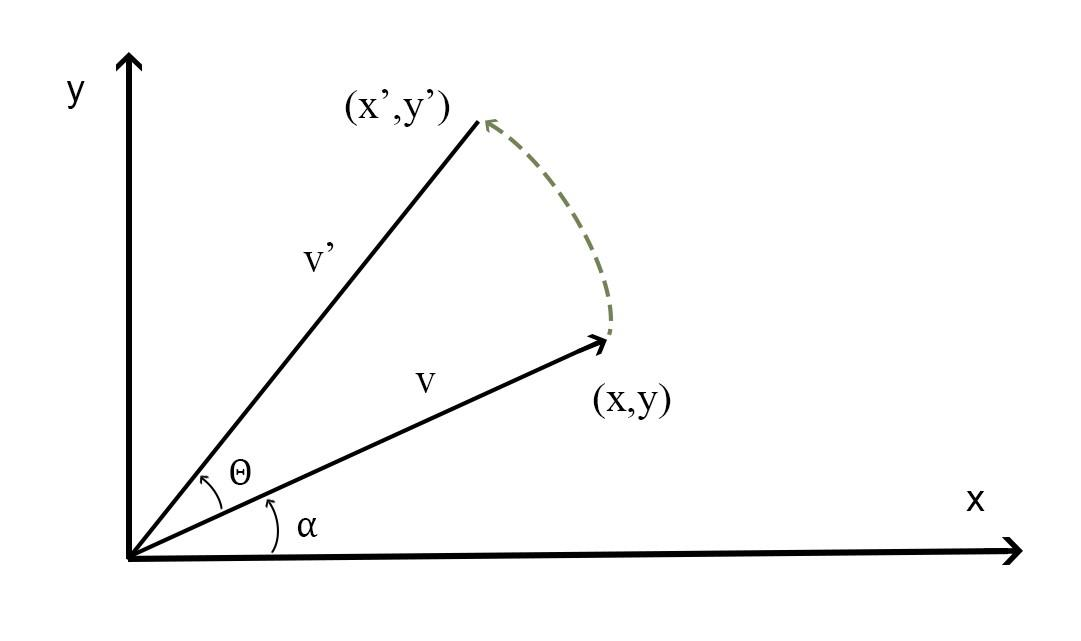
\includegraphics[width=0.60\textwidth]{Pictures/TLfig20.jpg}
    \caption{Transformación de rotación }
    \label{TLfig20}
\end{figure}

\bigskip

\begin{example}
\label{Simetria}
En $\mathbb{R}^3$, consideramos el subespacio $V_1$ correspondiente al  plano $xy$. Si $B= \left\{\vec{e}_1,\vec{e}_2,\vec{e}_3\right\}$ es la base canónica, y $S$ la transformación lineal que  para cada vector $\vec{v}$ da el vector  simétrico con respecto al plano $xy$, como se muestra en la Figura \ref{TLfig30},  se tiene  que  

$$ S(\vec{e}_1)=\vec{e}_1, \quad S(\vec{e}_2)=\vec{e}_2, \quad S(\vec{e}_3)= - \vec{e}_3.$$

Por lo tanto su matriz con respecto a  la base canónica es

$$S=\left(\begin{array}{ccc} 1 & 0 &  0\\
0 &  1  &  0\\
0 &  0  &  -1
\end{array}\right)$$
\end{example}
\begin{figure}
    \centering
    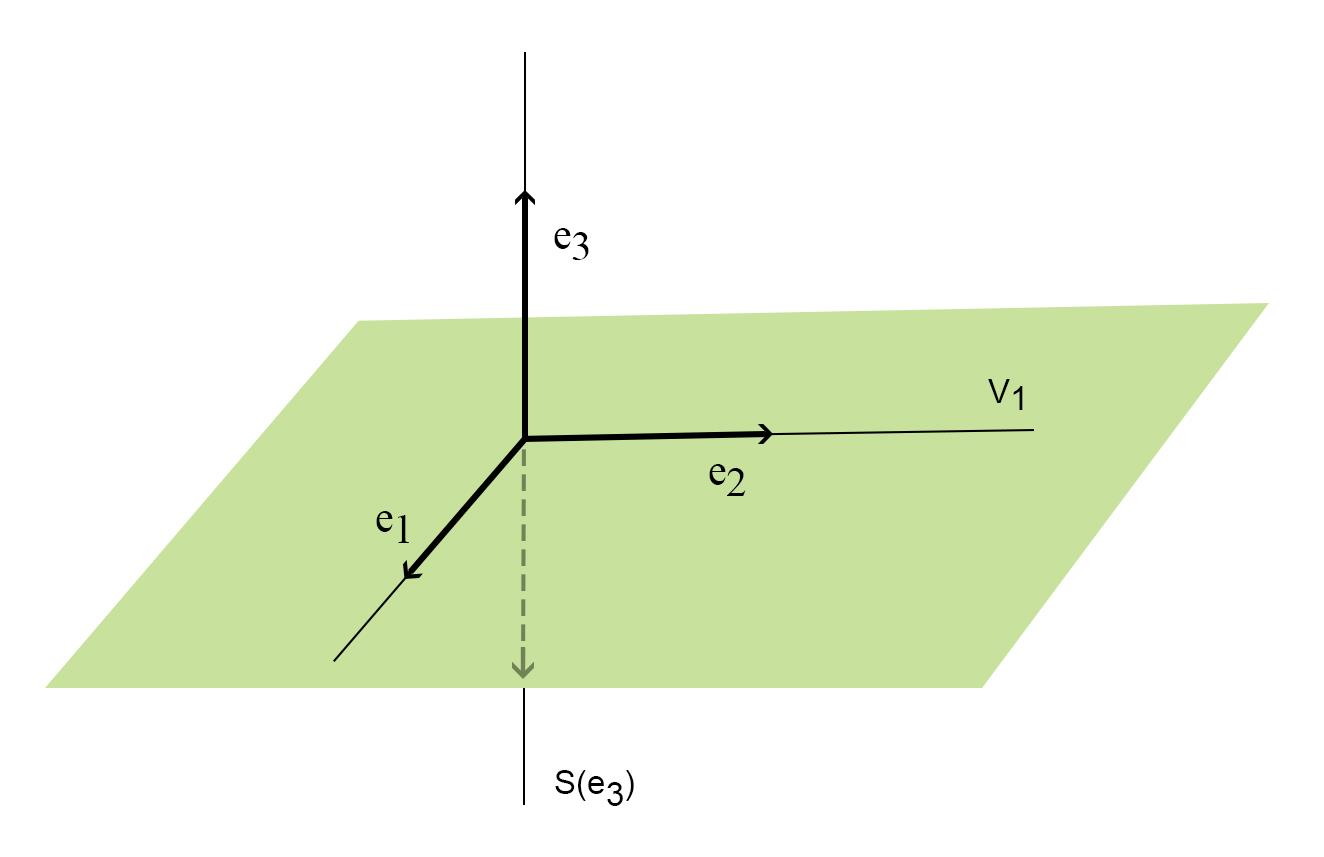
\includegraphics[width=0.90\textwidth]{Pictures/TLfig30.jpg}
    \caption{Simetria con respecto al plano $xy$ }
    \label{TLfig30}
\end{figure}
%(agregar figura pág 256 EH)




\begin{remark}
$\\$
Si se quiere  hallar la matriz que corresponde a la transformación lineal que a cada vector le hace corresponder el vector   simétrico  con respecto a un plano cualquiera, es conveniente   hallar  una base del plano ${ \vec{u}_1, \vec{u}_2}$ y un vector $\vec{u}_3 $ perpendicular.  Así, en la base $\{ \vec{u}_1, \vec{u}_2, \vec{u}_3\} $, la matriz de la simetría con respecto al plano es la misma  que la matriz del Ejemplo \ref{Simetria}. Una vez obtenida la matriz se realiza el cambio de base a la base deseada.
%\hfill$\blacktriangle$
\end{remark}

\bigskip


\begin{example}
De acuerdo a la corolario anterior, para hallar la matriz correspondiente a la simetría con respecto al plano $x+y+z=0$ (Figura \ref{TLfig300}). se busca una base del plano (como $x=-y-z$, los vectores en el plano son de la forma $(-y-z,y,z)=y(-1,1,0)+z(-1,0,1)$, es decir que  los vectores $\vec{u}_1=( -1,1,0)$  y $\vec{u}_2=( -1,0,1)$ son una base del mismo ). Y un vector perpendicular es  $\vec{u}_3=( 1,1,1)$.
En esa  base $\{ \vec{u}_1, \vec{u}_2, \vec{u}_3\} $ la matriz de la simetría con respecto al plano $x+y+z=0$ es, 
entonces,  

$$\left(\begin{array}{ccc} 1 & 0 &  0\\
0 &  1  &  0\\
0 &  0  &  -1
\end{array}\right)$$
\end{example}

\bigskip

\begin{figure}
    \centering
    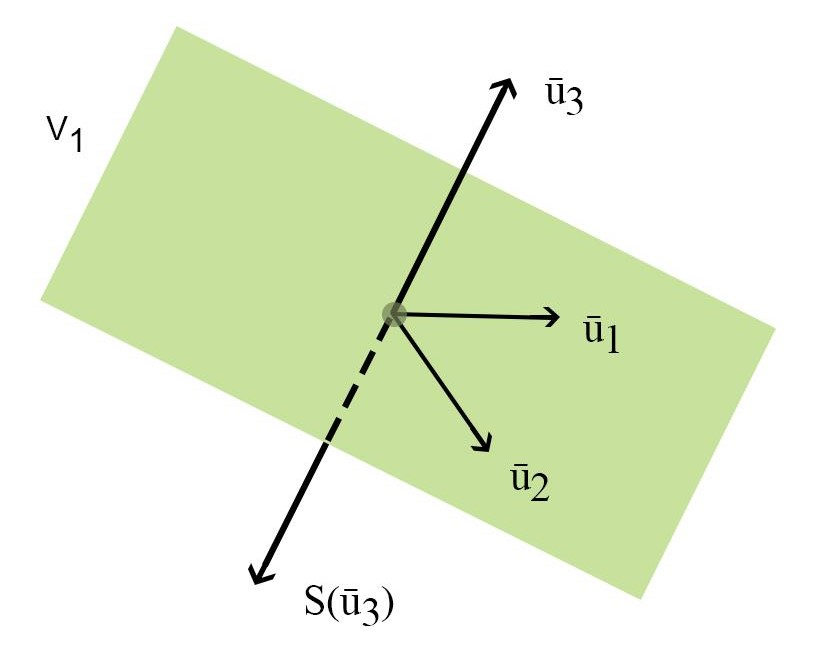
\includegraphics[width=0.65\textwidth]{Pictures/TLfig40.jpg}
    \caption{Simetría respecto al plano $x+y+z=0$ }
    \label{TLfig300}
\end{figure}

\bigskip

\bigskip

Si en los espacios vectoriales $V$ y $W$, de dimensiones finitas $n$ y $m$, respectivamente, se fijan bases, existe una correspondencia biunívoca entre las transformaciones lineales de $V$ en $W$ y el conjunto de las matrices $K^{m \times n}$ (de orden $m \times n$) sobre el cuerpo $K$. Puesto que el conjunto $K^{m \times n}$, posee una estructura de espacio vectorial, también  tiene esa estructura el conjunto de todas las transformaciones lineales entre dos espacios vectoriales sobre el mismo cuerpo $K$. A ese espacio vectorial se lo  denomina $L(V,W)$.


\bigskip

%Las  dos operaciones que le dan estructura de espacio vectorial son:





%Si $T$ y $T ^\prime$ son elementos de $L(V,W)$, definimos la suma mediante

%$$(T+ T ^\prime)(\vec{v})=T(\vec{v})+T^ \prime(\vec{v})~~ para ~todo ~ \vec{v}\in V$$

%Si $T$ es un elemento de $L(V,W)$ y $c$ es un elemento de $K$, se define la multiplicación de $c$ por $T$ mediante

%$$(cT)(\vec{v})=c(T(\vec{v}))~~ para ~todo ~ \vec{v}\in V$$



%Las operaciones recién definidas tienen ciertas propiedades que coinciden con las enumeradas para matrices, y se resumen en el teorema a %continuación:
\bigskip


\bigskip


\begin{corollary}
\label{TEO2}
Sean $V$ y $W$ dos espacios vectoriales sobre un mismo cuerpo $K$; el conjunto $L(V,W)$ de las aplicaciones lineales entre $V$ y $W$, es un espacio vectorial sobre el cuerpo $K$. 

\begin{proof}
\begin{itemize}
\item
Suma. 

Dadas $T_1$ y $T_2$ $ \in  L(V,W)$, se define $T_1+T_2$, $T_1+T_2: V \rightarrow W$  como 
$$ (T_1+T_2)(\vec{v})=  T_1(\vec{v})  +T_2(\vec{v}) \qquad \forall  \vec{v}\in V $$

Veamos que $T_1+T_2$ es una transformación lineal



\begin{itemize}
\item $(T_1+T_2)(\vec{v} + \vec{w} ) = T_1(\vec{v} + \vec{w} )  +  T_2(\vec{v} + \vec{w} )$

$= T_1(\vec{v}) +T_1( \vec{w} )  +  T_2(\vec{v} )+ T_2(\vec{w} )$

$=(T_1+T_2)(\vec{v})     + (T_1+T_2) (\vec{w})$

\bigskip

\bigskip

\item 
$ (T_1+T_2)( \alpha \vec{v})=  T_1( \alpha \vec{v}) + T_2( \alpha \vec{v}) $ 

$=  \alpha T_1( \vec{v}) + \alpha T_2( \vec{v}) $

$= \alpha (T_1( \vec{v}) +  T_2( \vec{v})) = \alpha (T_1 +  T_2)( \vec{v}) $
\end{itemize}

\bigskip

\bigskip

\item
Producto por escalares. 

Dada $T \in L(V,W)$ y $\alpha \in K$, se define  $(\alpha T)$, $(\alpha T): V \rightarrow W$ como 

$$ (\alpha T)(\vec{v})=  \alpha T ( \vec{v}) $$


Veamos que $(\alpha T)$ es una transformación lineal

\bigskip

\begin{itemize}
\item $(\alpha T)(\vec{v} + \vec{w} ) = \alpha (T(\vec{v} + \vec{w} ))$

$= \alpha (T(\vec{v}) + T(\vec{w} ))=  \alpha T(\vec{v}) + \alpha T(\vec{w} )    $

$=(\alpha T)(\vec{v}) + (\alpha T)(\vec{w} )$


\bigskip

\item 
$ (\alpha T)( \beta  \vec{v})=  \alpha (T( \beta  \vec{v})) $ 

$= \alpha (  \beta   T(  \vec{v})) =  (\alpha  \beta)   T(  \vec{v})  $

$= \beta (\alpha T(  \vec{v}))=  \beta (\alpha T)(  \vec{v})  $
\end{itemize}


\end{itemize}

\end{proof}
\end{corollary}



\bigskip

\bigskip

Como toda transformación lineal puede representarse mediante una matriz y recíprocamente, se tiene el siguiente resultado:


\bigskip

\bigskip

\begin{corollary}
\label{TEO3}

Sean $V$ y $W$ espacios vectoriales de dimensiones $n$ y $m$, respectivamente, entonces, el espacio vectorial de las transformaciones lineales del espacio vectorial  $V$ al espacio vectorial $W$, $L(V,W)$,  tiene dimensión $m\times n$.



\begin{proof}
 Se puede ver   en el libro de  E. Hernández \cite{hernandez}. En ella se construye una base de $L(V,W)$. También puede demostrarse  a partir de la correspon-\ dencia biyectiva entre el espacio vectorial de las matrices $K^{m \times n}$ (de dimensión $m \times n$) y  $L(V,W)$.

\end{proof}

\end{corollary}




\begin{remark}
\begin{itemize}
\item
Si $V$ y $W$ coinciden escribimos $L(V)$ en lugar de $L(V,V)$.

\item


La matriz de la aplicación lineal \textit{suma} coincide con la suma de las matrices de cada una de las aplicaciones y la matriz de la aplicación lineal $cT$ coincide con el producto de la matriz $T$ por el escalar $c$. Si llamamos $M(T)$ a la matriz de la aplicación lineal $T$, esto se escribe 

$$M(T+ T ^\prime) = M(T)+M(T ^\prime) \quad \text{y} \quad  M(cT) = cM(T),~ ~ c\in K$$ 
\end{itemize}
%\hfill$\blacktriangle$
\end{remark}


\bigskip

\bigskip

Se verá a continuación que la composición de funciones usual puede realizarse entre dos transformaciones lineales y el resultado es otra transformación lineal.\index{Composición de transformaciones lineales }


\bigskip


\begin{theorem}
\label{Prop342}


Sean $V$, $W$ y $X$ espacios vectoriales sobre el cuerpo $K$. Sean $T\in L(V,W)$ y $T ^\prime\in L(W,X)$. Entonces 

$$ T ^\prime \circ T  \in L(V,X)$$

\begin{proof}

Sean $\vec{v}_1,\vec{v}_2  \in V      $, entonces

\bigskip

$(T ^\prime \circ T )( \vec{v}_1 + \vec{v}_2)= T ^\prime ( T ( \vec{v}_1+ T(\vec{v}_2))= T ^\prime ( T ( \vec{v}_1) )+  T ^\prime (  T(\vec{v}_2)) $

\bigskip

$= (T ^\prime \circ T )( \vec{v}_1)+  (T ^\prime \circ T )( \vec{v}_2) $

Análogamente,

\bigskip


$(T ^\prime \circ T )( \alpha \vec{v})= T ^\prime ( T ( \alpha \vec{v})) = T ^\prime (\alpha T (  \vec{v}))= \alpha  (T ^\prime  \circ T )( \alpha \vec{v})    $
\end{proof}
\end{theorem} 

\bigskip


\begin{theorem}
 Si los espacios $V$, $W$ y $X$ tienen dimensión finita y si denotamos por $M(T)$, $M(T ^\prime)$ y $M(T ^\prime o T)$ las matrices de $T$, $T ^\prime$ y $T ^\prime o T $, respectivamente, con respecto a las bases de antemano fijadas, se tiene el siguiente resultado:

$$M(T ^\prime o T)= M(T ^\prime)M(T)$$

%{\textbf{NOTA:}}  Se puede ver la demostración en el Eugenio Hernández, pág. 261.

\begin{proof}
\begin{equation}
\label{Tej}
T(\vec{e}_j)=\sum_{i=1}^{m}a_{ij}\vec{f}_i,~~ j=1,2 \cdots,n
\end{equation}
donde $a_{ij}$ son los elementos de la matriz $M(T)$.

\bigskip

Sean $\left\{\vec{e}_1,\vec{e}_2,\cdots, \vec{e}_n\right\}$, $\left\{\vec{f}_1,\vec{f}_2,\cdots, \vec{f}_m\right\}$  y $\left\{\vec{g}_1,\vec{g}_2,\cdots, \vec{g}_p\right\}$  bases  de $V$, $W$ y $X$, respectivamente. 
En la $i$-ésima columna de la matriz   $M(T ^\prime o T)$    están las coordenadas del vector $(T ^\prime o T)(\vec{e}_i)$ con respecto a la base $g_k$.

\begin{eqnarray*}
T ^\prime (T(\vec{e}_i))&= &T ^\prime ( \sum_{j=1}^{m}a_{ji}\vec{f}_j)\\
&= &\sum_{j=1}^{m}a_{ji} T ^\prime ( \vec{f}_j)\\
&= &\sum_{j=1}^{m}a_{ji} \sum_{k=1}^{p}b_{kj}  \vec{g}_k\\
&= &\sum_{k=1}^{p}\sum_{j=1}^{m}b_{kj} a_{ji} \vec{g}_k
\end{eqnarray*}
\bigskip
\noindent
donde $b_{ij}$ son los elementos de la matriz $M(T ^\prime)$.

Esto prueba que $  \sum_{j=1}^{m}b_{kj} a_{ji}$ es el elemento que ocupa el lugar $(k,i)$ de la matriz $ M(T ^\prime o T)$ y este valor coincide con el elemento $(k,i)$ del producto de las matrices $M(T ^\prime)$ y $M(T)$.

\end{proof}
\end{theorem} 

\bigskip

\begin{remark}
El resultado anterior se generaliza para el caso de una sucesión de tranformaciones lineales, $T_i$, $i=1, \cdots k$ aplicadas a un vector $\Vec{v}$. Se tendrá entonces que resulta equivalente a aplicar a $\Vec{v}$ una única matriz $T$ tal que   $$M(T)= M(T_k)M(T_{k-1}) \cdots M(T_{2}) M(T_{1})  .$$
%\hfill$\blacktriangle$
\end{remark}

\bigskip

\section{Transformaciones lineales inyectivas y suryectivas.}\index{Transformación lineal inyectiva}\index{Transformación lineal suryectiva}
\label{TLIYS}

Sean $V$ y $W$ dos espacios vectoriales sobre el mismo cuerpo $K$ y $T$ una aplicación lineal de de $V$ en $W$. Recordamos que $T$ es inyectiva si 
$T(\vec{x})=T(\vec{y})$ implica $\vec{x}=\vec{y}$ y $T$ es suryectiva si para todo $\vec{y} \in W$ existe $\vec{x} \in V$ tal que $T(\vec{x})=\vec{y}$ (o equivalentemente $T(V)=W$, donde $T(V)$ denota la imagen de $V$ mediante $T$). Finalmente recordamos que $T$ es \textit{biyectiva} si es a la vez inyectiva y suryectiva.


\begin{remark}\index{Monomorfismo}\index{Epimorfismo}\index{Isomorfismo}
$\\$
En el caso de tranformaciones lineales cada uno de los tipos anteriores recibe un nombre especial: una aplicación lineal \textit{inyectiva} recibe el nombre de \textit{monomorfismo}; si es \textit{suryectiva }se le da el nombre de \textit{epimorfismo}; finalmente si la aplicación es \textit{biyectiva} se dice que es un \textit{isomorfismo}.
%\hfill$\blacktriangle$
\end{remark}




Encontraremos ahora condiciones sencillas que sirvan para determinar si una aplicación lineal es de cualquiera de los tipos anteriores. Comenzaremos con las aplicaciones inyectivas, y para ello necesitamos definir el concepto de \textit{núcleo }de una aplicación lineal.

\section{Núcleo e imagen  de una  transformación  lineal.}
\label{Núcleo e Imagen}

\bigskip

\begin{definition}\label{Nucleo}\index{Núcleo  de una transformación lineal}
Dada una aplicación lineal $T: V \rightarrow W$, 
 definimos el \textit{núcleo} de $T$, que se denota por $N(T)$ (o $Ker(T)$, del inglés \textit{kernel} significa núcleo), como el conjunto de todos los $\vec{v} \in V$ tal que $T(\vec{v})=\vec{0}$, es decir 


$$N(T)=\left\{\vec{v}~ \in V, / T(\vec{v})=\vec{0} \right\}$$

\end{definition}

\bigskip

\bigskip

El subconjunto $N(T)$ nunca es vacío, ya que $\vec{0} \in N(T)$ y esto se deduce de que $T(\vec{0})=\vec{0}$ como ya fue demostrado. Se tiene además, el siguiente resultado:

\bigskip


\bigskip

\begin{theorem}
\label{Prop343}


Si $T: V \rightarrow W$ es una aplicación lineal entre espacios vectoriales, $N(T)$ es un subespacio vectorial de $V$.

\begin{proof}

Esta propiedad  es consecuencia de la Proposición \ref{Prop33}. Por definición $N(T)$ es la preimagen de $\vec{0}_W$ que es un subespacio de $W$.
\end{proof}
\end{theorem} 



%\begin{thm}
%\label{Prop344}

%Si $T: V \rightarrow W$ es una aplicación lineal entre espacios vectoriales. La imagen mediante $T$ de cualquier subespacio vectorial de %$V$ es un subespacio vectorial de $W$.

%\begin{proof}
%\end{proof}
%\end{thm} 

%(ver Prop. 4 pág. 44)

\bigskip


\begin{theorem}
\label{Prop345}

Una aplicación lineal  $T: V \rightarrow W$ es inyectiva si y sólo si  $N(T)=\left\{\vec{0} \right\}$.



\begin{proof}
\begin{itemize}
\item
Si $T$ es inyectiva se tiene que $ T(\Vec{v})=T(\Vec{v}^{\prime})$ implica que $\vec{v}=\Vec{v}^{\prime}$. Si $\exists ~ \Vec{v} ~\in N(T)$  tal que  $T(\vec{v})=\vec{0}  $ como $T(\vec{0})=\vec{0}$ resulta $\vec{v}=\vec{0}$.
\item
Para ver que $T$ es inyectiva suponemos $\exists $ $\vec{v}$ y $\vec{v}^{\prime}$, tales que $ T(\vec{v})=T(\vec{v}^{\prime})$.

Por ser $T$ una transformación lineal $T(\vec{v})=T(\vec{v}^{\prime})= T( 
  \vec{v}-\vec{v}^{\prime})$, y si $T( \vec{v}-\vec{v}^{\prime})= \vec{0} $, entonces,  $\vec{v}-\vec{v}^{\prime} ~ \in ~ N(T)$. 
  
  Como $N(T)=\left\{\vec{0} \right\}$, se tiene que $\vec{v}=\Vec{v}^{\prime}$ y por lo tanto $T$ es inyectiva.
 
  
\end{itemize}
\end{proof}
\end{theorem} 

\bigskip

\begin{example}
Para la proyección ortogonal $P$   de la Figura \ref{figproyxy} (Ejemplo \ref{proyxy}), $$N(P) = \{(x,y,z) \in \mathbb{R}^3 \text{  tales que  } P(x,y,z)=(x,y,0)=(0,0,0) \}.$$ O sea $N(P)= \{ (0,0,z), ~z \in \mathbb{R} \}$ o sea todo el eje $z$. Por  la Proposición \ref{Prop345}, se tiene que  $P$  no es inyectiva (intuitivamente se ve que muchos vectores de 
$\mathbb{R}^3$  dan el mismo vector al proyectarlos  sobre el plano $xy$).
Además, se tiene que  las dimensiones  de $N(P)$ y de la $Im(P)$ son $1$ y $2$, respectivamente, suman $3$, que es la dimensión de $\mathbb{R}^3$. 
\end{example}

\bigskip

\begin{remark}
Si bien las soluciones de un sistema $A\vec{X}=\vec{b}, ~  \vec{b} \neq \vec{0}$  son un subconjunto pero no un subespacio de    $\mathbb{R}^n$ (ver Observación 
 \textcolor{blue}{{\fontfamily{qcr}\selectfont{i}}} en \ref{SHSNH}), toda solución puede expresarse de la forma $\vec{X}= \vec{X}_{NH} + \vec{X}_{H}$, donde  $\vec{X}_{NH}$ es solución de $A\vec{X}=\vec{b}$ mientras que  $\vec{X}_{H} \in Nul(A)$.
Esto sale porque si $\vec{X}_{NH}$ es solución de $A\vec{X}=\vec{b}$, $A(\vec{X}_{NH}+\vec{X}_{H})=  A\vec{X}_{NH}+ A\vec{X}_{H}=   \vec{b}+ \vec{0}= \vec{b} $ y si $\vec{X}$ es otra solución de $A\vec{X}=\vec{b}$, entonces $A(\vec{X}- \vec{X}_{NH})= A\vec{X}- A\vec{X}_{NH}=\vec{b}-\vec{b}=\vec{0} $, de donde $\vec{X}- \vec{X}_{NH}  \in Nul(A)$ y por lo tanto $\vec{X}=  \vec{X}_{NH} +\vec{X}_{H} $.

\bigskip

Como ejemplo se deja al lector verificar que la solución del sistema no homogéneo
\begin{equation} 
\left\{ \begin{array} {ccccl} \nonumber
                    x + y + w&\ =&1     \\
                     2x+3y+z+2w &\ = &1  
                    \end{array}
           \right.
\end{equation}

\bigskip
\noindent
es $\vec{X}=  \vec{X}_{NH} +\vec{X}_{H}= (2,-1,0,0)+ \alpha (1,-1,1,0) + \beta (-1,0,0,1) $ con $\alpha$ y $\beta$ $ \in \mathbb{R}$.
\hfill$\blacktriangle$
\end{remark}

\bigskip

\bigskip


Como se demostró en la Proposición \ref{Prop32}, la imagen de una transformación lineal $T$ es un subespacio. En el teorema que sigue se enuncia la relación que existe entre las dimensiones  del núcleo de $T$,  de la imagen de $T$ y la dimensión de $V$:

\bigskip



\begin{corollary}
    \label{Prop346}

Sean $V$ y $W$ dos espacios vectoriales de los cuales $V$ es de dimensión finita y  $T: V \rightarrow W$ es  una aplicación lineal. Entonces

$$ dim(N(T))+dim(Im(T))=dim(V).$$


\begin{proof}
Sea  $n=dim(V)$ y $k=dim(N(T))$,  

\bigskip
\noindent
si $k=n$, entonces $T$ es la aplicación nula y la $dim(Im(T))=0$. Por lo tanto el teorema vale.

\bigskip

Si $k=0$, entonces $T$ es un monomorfismo. Si $B$ es una base de $V$, $T(V)$ es base de la $Im(T)$. Luego la $dim(Im(T))=dim(V)$ y el teorema vale.

\bigskip

Supongamos que $0<k<n$ y sea $ \left\{\vec{v}_1,\vec{v}_2,\cdots, \vec{v}_k\right\}$  una base de $N(T)$. Sean $\vec{v}_{k+1},\vec{v}_{k+2},\cdots, \vec{v}_n$ tales que $ \left\{\vec{v}_1,\vec{v}_2,\cdots, \vec{v}_k, \vec{v}_{k+1},\vec{v}_{k+2},\cdots, \vec{v}_n    \right\}$ es una base de $V$.

\bigskip

Veamos que $ \left\{T(\vec{v}_{k+1}),T(\vec{v}_{k+2}),\cdots, T(\vec{v}_n )   \right\}$  es una base de $Im(T)$. 

\bigskip

En ese caso se tendrá que $dim(N(T))+dim(Im(T))=k + (n-k) = n= dim(V)$.

\bigskip

\begin{itemize}
    \item 
    Si $\vec{w}\in Im(T)$, $ \quad \exists \quad \vec{v} \in V $ tal que $T( \vec{v}) = \vec{w}$. 
    
    Como $\vec{v}= \sum_{j=1}^n  c_j \vec{v}_j $,  $\vec{w}=T(\vec{v})= \sum_{j=1}^n  c_j T(\vec{v}_j )= \sum_{j=k+1}^n  c_j T(\vec{v}_j )$,   ya que $ \left\{\vec{v}_1,\vec{v}_2,\cdots, \vec{v}_k\right\}$  es una base de $N(T)$. 
    
    Entonces, 
    $ \left\{T(\vec{v}_{k+1}),T(\vec{v}_{k+2}),\cdots, T(\vec{v}_n )   \right\}$  es un sistema de genera-\ dores de $Im(T)$.
    
    
   \bigskip 
    
    \item 
    Para ser si en un conjunto linealmente independiente, supongamos 
    
    $ \sum_{j=k+1}^n  c_j T(\vec{v}_j ) = \vec{0}=    T( \sum_{j=k+1}^n   c_j \vec{v}_j )    $. Entonces,
    
    $ \sum_{j=k+1}^n   c_j \vec{v}_j \in ~ N(T) $.  Como $ \left\{\vec{v}_1,\vec{v}_2,\cdots, \vec{v}_k\right\}$ es una base de $N(T)$, existen escalares $c_1, c_2, \cdots, c_k$ tales que 
    
    \bigskip
    
    $ \sum_{j=k+1}^n   c_j \vec{v}_j =   \sum_{j=1}^k   c_j \vec{v}_j  $

     \bigskip
\noindent
    que puede reescribirse
    
    \bigskip
    
    $    \sum_{j=1}^k  (- c_j)  \vec{v}_j + \sum_{j=k+1}^n   c_j \vec{v}_j = 0$
    
    
    \bigskip
    
Se tiene que $c_i=0$, $ \forall  ~ 1 \le i \le n$, 

por ser $ \left\{\vec{v}_1,\vec{v}_2,\cdots, \vec{v}_k, \vec{v}_{k+1},\vec{v}_{k+2},\cdots, \vec{v}_n    \right\}$  una base de $V$. En parti-\ cular $c_i=0$, $ \forall  ~  k+1 \le i \le n$. Luego $ \left\{T(\vec{v}_{k+1}),T(\vec{v}_{k+2}),\cdots, T(\vec{v}_n )   \right\}$ es un conjunto linealmente independiente.   
\end{itemize}
\end{proof}
\end{corollary}
\bigskip

\begin{example}
Se  verificará el teorema anterior para la transformación lineal $T:\mathbb{R}^5 \rightarrow \mathbb{R}^3 $, dada por $T ((z_1,z_2, \cdots, z_5)) = A (z_1,z_2, \cdots, z_5)^T$, donde $A$ es la matriz (ver Observación 
 \textcolor{blue}{{\fontfamily{qcr}\selectfont{i}}} al final de  la Sección \ref{AyT}).





$$A= \left(   \begin{array}{ccccc} 1 & 1 & 1 & 1 & 1 \\ 0 & 1 & 0 & -1 & 1 \\ 1 & 0 & 1 & 2 & 0 \end{array} \right )$$

En primer lugar, se resuelve el sistema homogéneo utilizando eliminación gaussiana (con la matriz ampliada):


   $$\left(   \begin{array}{cccccc} 1 & 1 & 1 & 1 & 1 & 0 \\ 0 & 1 & 0 & -1 & 1 & 0 \\ 1 & 0 & 1 & 2 & 0 & 0\end{array} \right )  \rightarrow  \left(   \begin{array}{cccccc} 1 & 1 & 1 & 1 & 1 & 0 \\ 0 & 1 & 0 & -1 & 1 & 0\\ 0 & -1 & 0 & 1 & -1 & 0\end{array} \right )\rightarrow  
   
   \rightarrow \left(   \begin{array}{cccccc} \underline{1} & 1 & 1 & 1 & 1 & 0 \\ 0 &\underline{1} & 0 & -1 & 1 & 0\\ 0 & 0 & 0 & 0 & 0 & 0\end{array} \right )$$
   
\bigskip
   
Al quedar solo dos pivotes, hay $2$ variables dependientes y $n-2=3$ variables independientes. Se tiene que dim(N(T))=3.


\bigskip

Para estudiar cuál es el subespacio que corresponde a la imagen de $T$, se debe hallar el subespacio de $\mathbb{R}^3$ que generan las columnas. Puede repetirse la eliminación anterior con término independiente $(x,y,z)$. 

\bigskip

$$\left(   \begin{array}{cccccc} 1 & 1 & 1 & 1 & 1 & x \\ 0 & 1 & 0 & -1 & 1 & y \\ 1 & 0 & 1 & 2 & 0 & z\end{array} \right )  \rightarrow  \left(   \begin{array}{cccccc} 1 & 1 & 1 & 1 & 1 & x \\ 0 & 1 & 0 & -1 & 1 & y\\ 0 & -1 & 0 & 1 & -1 & z-x\end{array} \right )\rightarrow  

\rightarrow \left(   \begin{array}{cccccc} \underline{1} & 1 & 1 & 1 & 1 & x \\ 0 & \underline{1} & 0 & -1 & 1 & y\\ 0 & 0 & 0 & 0 & 0 & z-x+y\end{array} \right )$$


\bigskip
Se tiene, entonces que $Im(T)= \left\{ (x,y,z)=( x,y, x-y) \right\}$, es el plano por el origen $z=x-y$, y

 \bigskip
 
$$dim(N(T))+dim(Im(T))= 3 + 2 = 5= dim(V),$$

\bigskip

\noindent
ya que $V= \mathbb{R}^5$.
 \end{example}

Para deducir algunas consecuencias del Teorema \ref{Prop346} es necesario hacer uso del concepto de \textit{rango}.\index{Rango de una matriz}

\bigskip

Sea $T$ una aplicación entre los espacios vectoriales $V$ y $W$, ambos de dimensión finita, $m$ y $n$ respectivamente. Sea $A$ la matriz de la aplicación lineal en dos bases cualesquiera de $V$ y $W$. Para encontrar el núcleo de $T$, $N(T)$, es necesario resolver el sistema homogéneo $A{\vec{\textbf{x}}}=\vec{0}$ (como se hizo en el ejemplo anterior). 

Si $r(A)$ es el rango  de la matriz $A$, se  obtienen, $r(A)$ soluciones dependien-\ tes y  $n-r(A)$ soluciones linealmente independientes. Es decir que

$$dim(N(T))=dim(V)-r(A)$$
\noindent
y comparando con el Teorema \ref{Prop346}, se tiene que 

$$dim(Im(T))=r(A)$$


\bigskip



Puesto que la dimensión de la $Im(T)$ no depende de las bases que se elijan en $V$ y $W$, de la igualdad anterior se deduce que  las matrices de la aplicación $T$ en cualquier base tienen el mismo rango.

\bigskip

Como consecuencia de lo anterior, es posible definir el \textit{rango de una transformación lineal} $T$, que escribiremos $r(T)$ como el rango de una cualquiera de sus
representaciones matriciales,  y resumir los resultados anteriores en el Corolario que sigue:


\bigskip

\textcolor{orange}{\textbf{Corolario}}
Sean $V$ y $W$ dos espacios vectoriales de los cuales $V$ es de dimensión finita y $T$ una transformación lineal, $T: V \rightarrow W$. Entonces


\begin{enumerate}

\item 

$T$ es inyectiva sí y sólo sí $r(T)=dim(V)$.


\item 

$T$ es suryectiva sí y sólo sí $r(T)=dim(W)$.


\end{enumerate}
%\end{remark}
%{\hfill{\tiny\ensuremath{\blacksquare}}

\bigskip


\bigskip
Por último se estudian las aplicaciones lineales entre espacios vectoriales de igual dimensión que son biyectivas. Se conocen como isomorfismos.
Supongamos que $V$ y $W$ son espacios vectoriales de dimensión finita, y que $T$ es un isomorfismo entre ellos. Del Corolario anterior deducimos que 

$$dim(V)=r(T)=dim(W)$$


\bigskip

Otras consecuencias  de  resultados anteriores se resumen en el teorema que sigue.

\bigskip

\bigskip

\begin{corollary}
\label{Prop347}





Sean $V$ y $W$ espacios vectoriales  de dimensión finita $n$  y  sea $T: V \rightarrow W$ es  una aplicación lineal. Las siguientes condiciones son equivalentes:

\bigskip

\begin{enumerate}

\item  $T$ es biyectiva


\item  $T$ es inyectiva

\item $N(T)=\left\{\vec{0} \right\}$

\item  $T$ es suryectiva

\item  El rango de $T$ es $n$

\end{enumerate}

\bigskip
%manual de latex pag30
\begin{proof}
Entre $2$, $3$, $4$ y $5$ se tienen las equivalencias siguientes:


\[ 
\begin{array}{ccc}
2 & \stk{Prop. \ref{Prop345}} & 3 \\
\Updownarrow{Corolario} &   &  \\
5  & \stk{Corolario}  & 4
\end{array}
\]
Además, $1  \rightarrow 2$ porque toda transformación biyectiva es inyectiva. Como $2$ y $4$ son equivalentes en este contexto y ambas implican $1$, se tiene que también  $2 \rightarrow 1$, y queda demostrado.
%$\stk{Prop. \ref{Prop345}}$
\end{proof}
\end{corollary} 


\bigskip


\bigskip

%\textbf{Isomorfismo}


Decimos que dos espacios vectoriales cualesquiera son \textit{isomorfos} si podemos encontrar un isomorfismo entre ellos. Para que esto ocurra entre espacios vectoriales de dimensión finita ya vimos que ambos han de tener la misma dimensión. El recíproco también es cierto.

\bigskip

\bigskip

\begin{corollary}
\label{Prop348}

Dado cualquier número natural $n$, todos los espacios vectoriales de dimensión $n$ sobre un mismo cuerpo son isomorfos.

\bigskip


\begin{proof}Sean $V$ y $W$ dos espacios vectoriales de dimensión $n$ con bases $\left\{\vec{e}_1,\vec{e}_2,\cdots, \vec{e}_n\right\}$ y $\left\{\vec{e}^{\prime}_1,\vec{e}^{\prime}_2,\cdots, \vec{e}^{\prime}_n\right\}$ respectivamente. 
Existe una transfor-\ mación lineal $T_1$, $T_1: V \rightarrow K^n$ definida de la forma siguiente:

\bigskip

Si $\Vec{v}=\sum_{i=1}^n \alpha_i \vec{e}_i$, $$T_1(\Vec{v})=(\alpha_1, \alpha_2, \cdots , \alpha_n) $$


\bigskip

Es decir que la transformación da el vector con las coordenadas de $\Vec{v}$.
Se demuestra fácilmente (y se deja al lector) que esta transformación es lineal, inyectiva y suryectiva. Al ser biyectiva, existe también su transformación inversa  (Proposición \ref{Prop347}).
Utilizando este isomorfismo de un espacio vectorial $V$ con $K^n$, se tiene que dos espacios cualesquiera de la misma dimensión sos isomorfos. Para encontrar la transformación entre $V$ y $W$ hay que  componer la transformación  $T_1$ entre V y  $K^n$ con la transformación $T_2$ entre   $K^n$ y el espacio vectorial $W$, $T_2: K^n  \rightarrow  W$.
Esta última está dada por

$$T_2(\alpha_1, \alpha_2, \cdots , \alpha_n) = \sum_{i=1}^n \alpha_i \vec{e}^{\prime}_i.$$

\bigskip

El isomorfismo entre $V$ y $W$ está dado por la transformación $$(T_2 \circ T_1)(\Vec{v})=T_2(T_1(\Vec{v}))=\Vec{w}= \sum_{i=1}^n \alpha_i \vec{e}^{\prime}_i  .$$
\end{proof}
\end{corollary} 

\bigskip

\begin{example}
 Aplicando el Teorema anterior, el isomorfismo entre $P_{\mathbb{R}}^{(2)}[t]$ y  $\mathbb{R}^3$  está dado por 
$$T( a_0 1+ a_1 t + a_2 t^2)= (a_0, a_1, a_2)^t,$$
mientras que el isomorfismo entre   $\mathbb{R}^3$ y las matrices simétricas  de $\mathbb{R}^{2\times2 }$  está dado por:
$$T(x,y,z)= \left(   \begin{array}{cc} x & y \\ y & z   \end{array} \right ).$$

\bigskip

Se consideraron  las bases canónicas de  $\mathbb{R}^3$, de $P_{\mathbb{R}}^{(2)}[t]$ y  de las matrices simétricas de $\mathbb{R}^{2\times2 }$,  espacios vectoriales de dimensión $3$. 
Se deja al lector la verificación de estos resultados.
\end{example}

\bigskip

\begin{remark}
Si $T$ es un isomorfismo entre dos espacios vectoriales $V$ y $W$ de dimensión $n$, por el Teorema \ref{Prop347}, su rango es $n$, y por lo tanto la matriz $M(T)$ de $T$ en cualesquiera bases de $V$ y $W$ es \textit{invertible}. Además, la inversa de $M(T)$ es la matriz de la aplicación inversa de $T$.
%\hfill$\blacktriangle$
\end{remark}


\bigskip

\begin{example}
%Ejemplos
%hojitas 15 y
Sean $V$ y $W$  dos espacios vectoriales de funciones,   de dimensión infinita:

 \bigskip
 
 $V=\{ f \in C^1[0,1] / f(0)=0 \}$ y $W=C[0,1] $.

 \bigskip
 
Sea la transformación 

\bigskip
 
 $D: V  \rightarrow W$ dada por $D(f)= f^{\prime}$. $D$ es una transformación lineal (En el Ejemplo \ref{ejderi} se vió para polinomios en $P_R^{(n)}[x]$) .
 \begin{itemize}
\item
$D$ es monomorfismo

Supongamos $D(f)=D(g)$, entonces $f^{\prime}= g^{\prime}$ o, en forma equivalente $(f-g)^{\prime}=0$. Entonces $f(x)-g(x)=cte$. Como $f(0)=g(0)=0$, se tiene que la $cte=0$, por lo tanto $f=g$. 
\item
$D$ es epimorfismo

Sea $g \in W$ y sea 

\[
f(x)=\int_0^x g(t)dt.
\]
Entonces, por el Teorema Fundamental del cálculo, $f \in C^1[0,1]$  y $f^{\prime}=g(x)$,  $ \forall  x \in [0,1]$.
Más aún, como \[
\int_0^0 g(t)dt=0, 
\]
\noindent
se tiene que 
$f(0)=0$. Por lo tanto, $\forall g \in W,  ~ \exists f \in V $  tal que $Df=g$. O sea $D$ es epimorfismo.
\end{itemize}
Resulta, entonces, que $V$ y $W$ son espacios isomorfos.
\end{example}

\bigskip

\index{González, Gabriela}
\begin{parchment}[Gabriela González] {Gabriela González es una física, investigadora y profesora argentina. Nació en 1965. Fue portavoz y coordinó durante seis años un equipo de mil especialistas, que trabajó en las detecciones de ondas gravitacionales efectuadas desde el proyecto LIGO (Ondas Gravitacionales con Interferómetro Láser, por sus siglas en inglés). En febrero de 2016 fue una de los cuatro científicos de LIGO que anunciaron la primera observación ondulatoria gravitacional, detectada en septiembre de 2015. Egresada de la Universidad Nacional de Córdoba y actual profesora en el departamento de física y astronomía de la Universidad de Louisiana, fue reconocida en 2016 como una de los diez científicos más destacados del mundo por la revista académica Nature. Además, a partir de 2018 forma parte de la Academia de Ciencias de Estados Unidos, institución de máximo prestigio internacional.  \cite{GabG} }
\end{parchment}


\bigskip

\section{Geometría de las transformaciones  lineales  de $\mathbb{R}^2$ en  $\mathbb{R}^2$   }
Se verán en esta sección algunas propiedades geométricas de las transformaciones lineales en el plano.
Dada la matriz 

$$A=\left(   \begin{array}{cc} a & b \\ c & d   \end{array} \right )$$
\noindent
la transformación $L: \mathbb{R}^2  \rightarrow \mathbb{R}^2$ dada por $L((x,y))=A (x,y)^t$ es $$L  \left( \left(  \begin{array}{c} x  \\ y  \end{array}    \right) \right )=\left(   \begin{array}{c} a x + by  \\ cx +  d y  \end{array} \right )$$ .
\begin{example}
 En la Figura \ref{TLfig50} se muestra la transformación que a cada vector le hace corresponder el simétrico respecto del eje $y$.
 \index{Reflexión}

 $$L  \left( \left(  \begin{array}{c} x  \\ y  \end{array}    \right) \right )= \left(   \begin{array}{cc} -1 & 0 \\ 0 & 1   \end{array} \right ) \left( \begin{array}{c} x  \\ y  \end{array} \right )     =\left(   \begin{array}{c} - x   \\ y  \end{array} \right )$$ .
\end{example}


\begin{figure}
    \centering
    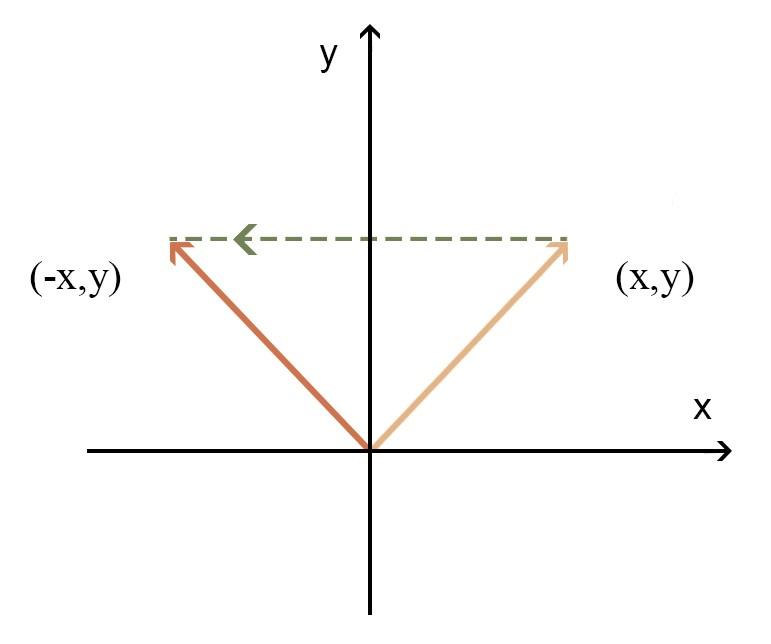
\includegraphics[width=0.50\textwidth]{Pictures/fig.13.jpg}
    \caption{Transformación de simetría (o reflexión) respecto del eje $y$ }
    \label{TLfig50}
\end{figure}

\begin{example}
 En la Figura \ref{TLfig60} se muestra la transformación que a cada vector le hace corrresponder el simétrico respecto del eje $x$

 $$L  \left( \left(  \begin{array}{c} x  \\ y  \end{array}    \right) \right )= \left(   \begin{array}{cc} 1 & 0 \\ 0 & -1   \end{array} \right )\left( \begin{array}{c} x  \\ y  \end{array} \right )      =\left(   \begin{array}{c} x   \\ -y  \end{array} \right )$$ .
\end{example}

\begin{figure}
    \centering
    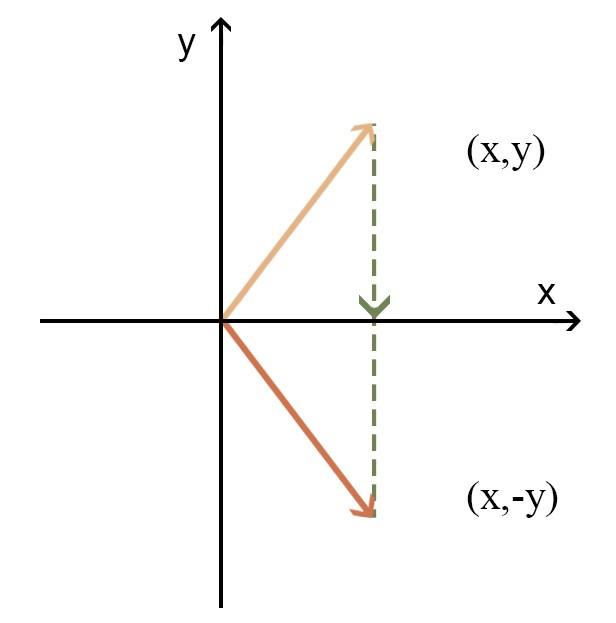
\includegraphics[width=0.50\textwidth]{Pictures/fig.14.jpg}
    \caption{Transformación de simetría respecto del eje $x$ }
    \label{TLfig60}
\end{figure}


\begin{example}
\label{proyejex}
 En la Figura \ref{fig36} se muestra la transformación que a cada vector le hace su proyección ortogonal sobre el eje $x$:

 $$L  \left( \left(  \begin{array}{c} x  \\ y  \end{array}    \right) \right )= \left(   \begin{array}{cc} 0 & 1 \\ 1 & 0   \end{array} \right ) \left( \begin{array}{c} x  \\ y  \end{array} \right )    =\left(   \begin{array}{c} x   \\ 0  \end{array} \right ).$$ 
\end{example}


\begin{figure}
    \centering
    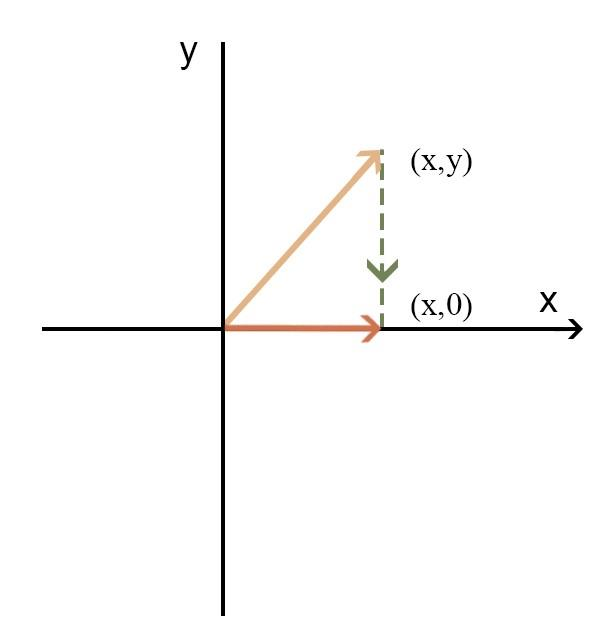
\includegraphics[width=0.50\textwidth]{Pictures/fig.36.jpg}
    \caption{Proyección ortogonal sobre el eje $x$ }
    \label{fig36}
\end{figure}



\begin{example}
\index{Reflexión}
 En la Figura \ref{TLfig77} se muestra la transformación que a cada vector le hace su reflexión  respecto de la recta  $y=x$:

 $$L  \left( \left(  \begin{array}{c} x  \\ y  \end{array}    \right) \right )= \left(   \begin{array}{cc} 0 & 1 \\ 1 & 0   \end{array} \right ) \left( \begin{array}{c} x  \\ y  \end{array} \right )     =\left(   \begin{array}{c} y   \\ x  \end{array} \right )$$ .
\end{example}
\begin{figure}
    \centering
    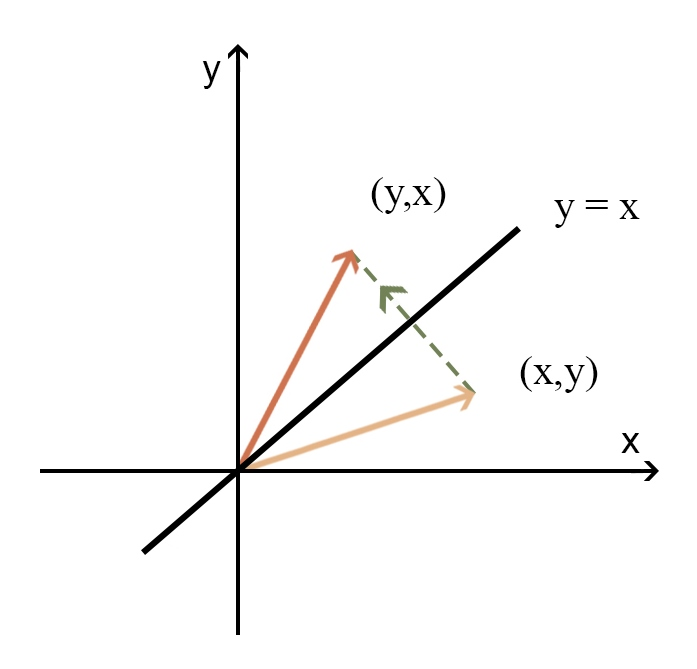
\includegraphics[width=0.50\textwidth]{Pictures/fig.17.jpg}
    \caption{Transformación de reflexión respecto de la recta $y=x$ }
    \label{TLfig77}
\end{figure}

\bigskip

\begin{remark}
 Otras  transformaciones se obtienen al multiplicar una de las  coordenadas por una constante $k$. Así el efecto es comprimir o dilatar en esa dirección, dependiendo si $k < 1$ o $k > 1$. También están las transformaciones llamadas de \textit{trasquillado}, dadas por matrices de la forma:

 $$L  \left( \left( \begin{array}{c} x  \\ y  \end{array}    \right) \right )= \left(   \begin{array}{cc} 1 & k \\ 0 &  0   \end{array} \right ) \left( \begin{array}{c} x  \\ y  \end{array} \right )     =\left(   \begin{array}{c} x+ky   \\ y  \end{array} \right ).$$
 %\hfill$\blacktriangle$
\end{remark}

Estos casos se analizarán en los ejercicios propuestos.


\begin{figure}
    \centering
    %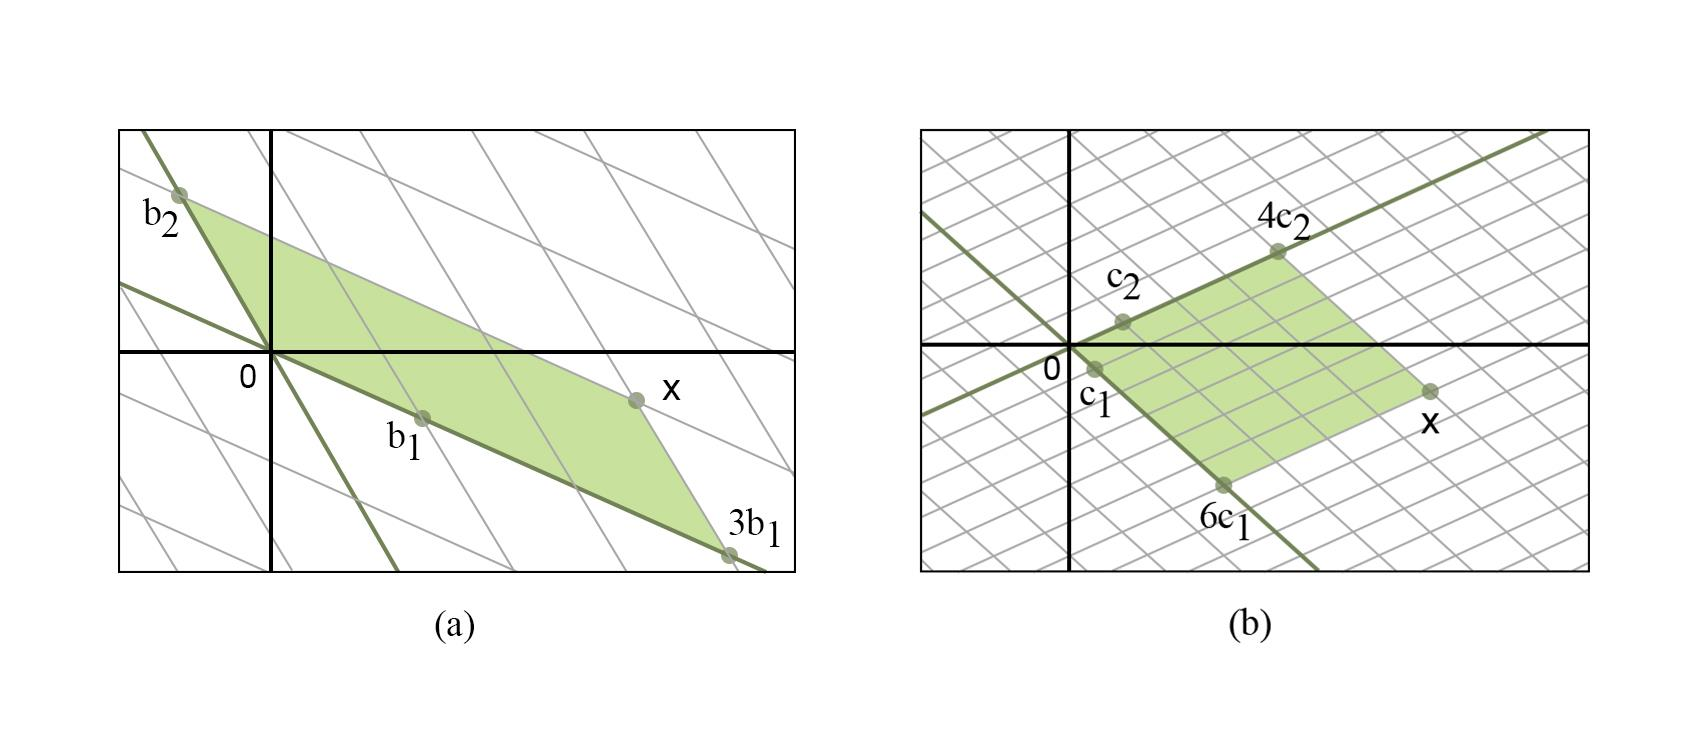
\includegraphics[width=0.90\textwidth]{Pictures/TLfig80.jpg}
    %\caption{Transformación de simetría respecto de la recta $y=x$ }
    \label{TLfig70}
\end{figure}


%\end{document}

\section{Cambio  de base para transformaciones  lineales}
 \label{cbaseTL}

Sean $V$ y $W$ dos espacios vectoriales sobre el mismo cuerpo $K$ de dimensiones $n$ y $m$, respectivamente. Sea $T$ una transformación lineal de $V$ en $W$ con matriz 

$$T=(a_{i,j})_{i,j=1,n}$$

\bigskip

\noindent
con respecto a las bases $B= \left\{\vec{e}_1,\vec{e}_2,\cdots, \vec{e}_n\right\}$  y $\bar{B}= \left\{\vec{f}_1,\vec{f}_2,\cdots, \vec{f}_n\right\}$   de $V$ y $W$, respectivamente. 

\bigskip


Si queremos conocer la matriz $T^{\prime} =(a_{i,j})_{i,j=1,n}$ de la misma aplicación $T$ respecto a dos nuevas bases  $B^{\prime}= \left\{\vec{e}^{\prime}_1,\vec{e}^{\prime}_2,\cdots, \vec{e}^{\prime}_n\right\}$  y $\bar{B^{\prime}}= \left\{\vec{f}^{\prime}_1,\vec{f}^{\prime}_2,\cdots, \vec{f}^{\prime}_n\right\}$   de $V$ y $W$, respectivamente, es necesario realizar los cambios de base adecuados en los espacios vectoriales  inicial y final, $V$ y $W$.



\bigskip


\noindent
Para seguir el razonamiento, veamos el diagrama siguiente

 %\begin{center}
 %    {\framebox{
 %         \parbox {8.5cm}{\begin{center} {$B= \left\{\vec{e}_1,\vec{e}_2,\cdots, \vec{e}_n\right\}$ \end{center}}}}   
%nd{center}
%
%newcommand{\stk}[1]{\stackrel{#1}
%{\longrightarrow}}
%\newcommand{\cT}{\mathcal{T}}
%\newcommand{\dwn}[1]{
%{\scriptstyle #1}\downarrow}
%\[
%\begin{array}{ccc}
%U       & \stk{G}  & \cT  U\\
%\dwn{\phi}  &      &  \dwn{\cT\phi}\\
%$B^{\prime}= \left\{\vec{e^{\prime}}_1,\vec{e}_2,\cdots, \vec{e}_n\right\}$  & \stk{\cT\phi\circ G\circ\phi}     &  \cT\phi(\cT U)
%\end{array}
%\]

\newcommand{\stk}[1]{\stackrel{#1}
{\Longrightarrow}}
\newcommand{\cT}{\mathcal{T}}
\newcommand{\dwn}[1]{
{\scriptstyle #1}\Uparrow}
\[
%\begin{center}
\begin{array}{ccc}
      V           & y=T(x)         &    W        \\\\
B= \left\{\vec{e}_1,\vec{e}_2,\cdots, \vec{e}_n\right\}    & \stk{a_{i,j}}  &  \bar{B}= \left\{\vec{f}_1,\vec{f}_2,\cdots, \vec{f}_n\right\} \\
\dwn{C}  &      &  \dwn{D} \\
B^{\prime}= \left\{\vec{e}^{\prime}_1,\vec{e}^{\prime}_2,\cdots, \vec{e}^{\prime}_n\right\}  & \stk{a^{\prime}_{i,j}}    &  \bar{B^{\prime}}= \left\{\vec{f}^{\prime}_1,\vec{f}^{\prime}_2,\cdots, \vec{f}^{\prime}_n\right\}
\end{array}
%\end{center}
\]

\bigskip

\bigskip

En el diagrama

\bigskip

\begin{itemize}
\item

$a_{ij}$ son los elementos de  la matriz de la transformación $T$ tomando la base $ B$ en $V$ y la base  $\bar{B}$ en $W$   
\item
$a^{\prime}_{ij}$ son los elementos de  la matriz de la transformación $T$ tomando la base $ B^{\prime}$ en $V$ y la base  $\bar{B}^{\prime}$ en $W$   \item
 $C$ y $D$ son las matrices del cambio de base de $B^{\prime}$ a $B$ y de $\bar{B^{\prime}}$ a $\bar{B}$, respectivamente.
\end{itemize}

\bigskip


Se tiene que $\vec{x}\in V$ puede escribirse de dos formas 

\bigskip

$$ x_1\vec{e}_1+x_2\vec{e}_2+\cdots +x_n\vec{e}_n = x^{\prime}_1\vec{e}^{\prime}_1+x^{\prime}_2\vec{e}^{\prime}_2+\cdots +x^{\prime}_n\vec{e}^{\prime}_n $$


\bigskip
e   $\vec{y}=T(\vec{x})$ también


\bigskip

$$ y_1\vec{f}_1+y_2\vec{f}_2+\cdots +y_n\vec{f}_n = y^{\prime}_1\vec{f}^{\prime}_1+y^{\prime}_2\vec{f}^{\prime}_2+\cdots +y^{\prime}_n\vec{f}^{\prime}_n $$


\bigskip

\bigskip

\bigskip

En primer lugar, se tiene que, 

\bigskip

\begin{eqnarray}
\label{yTx}
\left(\begin{array}{c} y_{1} \\ y_{2}  
\\  y_3 \\ \cdots \\ y_{n} 
\end{array} \right)=T\left(\begin{array}{c} x_{1} \\ x_{2}  
\\  x_3 \\ \cdots \\ x_{n} 
\end{array} \right)
\end{eqnarray}

\bigskip

\noindent
y de acuerdo a los cambios de base en un mismo espacio vectorial que se estudiaron antes, 


$$\left(\begin{array}{c} x_{1} \\ x_{2}  
\\  x_3 \\ \cdots \\ x_{n} 
\end{array} \right)=C\left(\begin{array}{c} x^{\prime}_{1} \\ x^{\prime}_{2}  
\\  x^{\prime}_3 \\ \cdots \\ x^{\prime}_{n} 
\end{array} \right)~~~~~~~~\left(\begin{array}{c} y_{1} \\ y_{2}  
\\  y_3 \\ \cdots \\ y_{n} 
\end{array} \right)=D\left(\begin{array}{c} y^{\prime}_{1} \\ y^{\prime}_{2}  
\\  y^{\prime}_3 \\ \cdots \\ y^{\prime}_{n} 
\end{array} \right)$$
\bigskip
mientras que, considerando las bases ${B^{\prime}}$ y   $\bar{B^{\prime}}$, se tiene que, 
\bigskip
\begin{eqnarray}
\label{yTpx}
\left(\begin{array}{c} y^{\prime}_{1} \\ y^{\prime}_{2}  
\\  y^{\prime}_3 \\ \cdots \\ y^{\prime}_{n} 
\end{array} \right)=T^{\prime}\left(\begin{array}{c} x^{\prime}_{1} \\ x^{\prime}_{2}  
\\  x^{\prime}_3 \\ \cdots \\ x^{\prime}_{n} 
\end{array} \right)
\end{eqnarray}
\bigskip



Sustituyendo en (\ref{yTx}),  se obtiene, 


$$D\left(\begin{array}{c} y^{\prime}_{1} \\ y^{\prime}_{2}  
\\  y^{\prime}_3 \\ \cdots \\ y^{\prime}_{n} 
\end{array} \right)=TC\left(\begin{array}{c} x^{\prime}_{1} \\ x^{\prime}_{2}  
\\  x^{\prime}_3 \\ \cdots \\ x^{\prime}_{n} 
\end{array} \right)$$

\bigskip

\noindent
y como $D$ es una matriz de cambio de base, tiene inversa, por lo tanto


$$\left(\begin{array}{c} y^{\prime}_{1} \\ y^{\prime}_{2}  
\\  y^{\prime}_3 \\ \cdots \\ y^{\prime}_{n} 
\end{array} \right)=D^{-1}TC\left(\begin{array}{c} x^{\prime}_{1} \\ x^{\prime}_{2}  
\\  x^{\prime}_3 \\ \cdots \\ x^{\prime}_{n} 
\end{array} \right)$$

\bigskip

\noindent
Comparando esta expresión con (\ref{yTx}) se obtiene, finalmente que 

$$T^{\prime}= D^{-1}TC,$$

\bigskip

\noindent
y es posible  calcular la matriz $T^{\prime}$ de la aplicación  $T$ con respecto a las bases $B^{\prime}$ y $\bar{B^{\prime}}$, conocidas la matriz $T$ de la misma aplicación con respecto a las bases $\bar{B}$ y $\bar{B^{\prime}}$ y las matrices $C$ y $D$ del cambio de base $B^{\prime}$ a $B$ y de $\bar{B^{\prime}}$ a $\bar{B}$, respectivamente.

\newpage

\begin{remark}\index{Matrices equivalentes} \index{Matrices semejantes}
\label{Obssemejanza}
\begin{itemize}
\item
Cuando entre dos matrices $T$ y  $T^{\prime}$ se tiene la relación 
$T^{\prime}= D^{-1}TC$, se dice que las matrices $T$ y  $T^{\prime}$ son \textit{equivalentes}  (  $D$ y $C$ son matrices invertibles). Y si  las matrices $D$ y $C$ coinciden, se dice que las matrices $T$ y  $T^{\prime}$ son  \textit{semejantes}.

\item
En muchos casos los espacios inicial $V$  y final $W$  de una transformación lineal coinciden, y se anota $T \in L(V)$. 

\item
Cuando  $B$ y $\bar{B}$ coinciden y $B^{\prime}$ y  $\bar{B^{\prime}}$ coinciden, la fórmula del cambio de base es más sencilla. Si $T$ es la matriz de la aplicación $T\in L(V)$ con respecto a la base $B$ de $V$, la matriz $T^{\prime}$ de la misma aplicación con respecto a una base $B^{\prime}$ de $V$  está dada por 


$$T^{\prime}=C^{-1}TC.$$
\noindent
donde $C$ es la matriz del cambio de base de $B^{\prime}$ a $B$.
Al tener esta relación entre las matrices,  por lo anterior, $T$ y  $T^{\prime}$ son \textit{semejantes}. 

\bigskip

\item

 Si $T^{\prime}=C^{-1}TC$, $Det(T^{\prime})=Det(T)$, ya que 
 \bigskip
 
 $Det(T^{\prime})= Det(C^{-1}TC)= Det(C)^{-1}Det(T).Det(C) \\ = Det(C^{-1}C)Det(T)= Det(I)Det(T)=Det(T)$.
 

\end{itemize}

% ejemplo hojita 15 y problema 6.5
\end{remark}
\bigskip

\bigskip


\begin{example}
\label{ejemplo217}

Si $B$ es la base canónica, $B^{\prime}=\{ (1,2), (2,3) \}$ y  

$$(T)_{B}= \left(   \begin{array}{cc} 6 & -2 \\ 6 &  -1   \end{array} \right )$$

se tiene que 
 $$(T)_{B^{\prime}}= \left(   \begin{array}{cc} 1 & 2 \\ 2 &  3   \end{array} \right )^{-1}\left(   \begin{array}{cc} 6 & -2 \\ 6 &  -1   \end{array} \right ) \left(   \begin{array}{cc} 1 & 2 \\ 2 &  3   \end{array} \right )   = \left(   \begin{array}{cc} 2 & 0 \\ 0 &  3   \end{array} \right )$$.
\end{example}
%\hfill$\blacktriangle$


\bigskip

\section{Espacio dual de un espacio Vectorial.}\index{Espacio dual}


Dado un espacio vectorial $V$ sobre un cuerpo $K$, podemos considerar el conjunto $L(V,K)$ de todas las transformaciones lineales de $V$ en el espacio vectorial  $K$ (de dimensión  $1$ sobre $K$). 

\bigskip


Este espacio vectorial es un caso particular del estudiado anteriormente ($L(V,W)$), y el Teorema \ref{TEO2} de la sección nos permite concluir que $L(V,K)$ es un espacio vectorial sobre $K$. Este espacio vectorial recibe el nombre de \textit{espacio dual} del espacio vectorial $V$  y para indicarlo se utiliza comúnmente el símbolo $V^*$, en lugar de $L(V,K)$. En otras palabras, $V^*$ es el espacio vectorial de todas las aplicaciones lineales de $V$ en $K$, también llamados funcionales lineales..



\bigskip



Los elementos de $V^*$ son transformaciones lineales. Si $V$ es un espacio vectorial de dimensión finita $n$, del  Teorema \ref{TEO3} se deduce que es espacio dual $V^*$  tiene dimensión $n$. El teorema que sigue exhibe una base $B^{*}$ asociada de manera única  y natural a una base $B$ de $V$. La demostración del  Teorema \ref{TEO3}, más general, fue citada. Se presenta a continuación la demostración para este caso particular.

\bigskip

\bigskip


\begin{corollary}
\label{basedual}
Sea $V$ un espacio vectorial de dimensión finita $n$ y  $B= \left\{\vec{e}_1,\vec{e}_2,\cdots, \vec{e}_n\right\}$ una base de  $V$. Existe una única base 

$$B^*= \left\{\varphi_1,\varphi_2,\cdots,\varphi_n\right\}$$
de $V^*$ tal que $\varphi_i(\vec{e}_i)=1$ para todo $i=1, \cdots,n$,   y $\varphi_j(\vec{e}_i)=0$  si $i\neq j$. 
Es decir, los elementos de la base dual de  $B$ satisfacen 
 $$\varphi_j(\vec{e}_i)= \delta_{ij}, \qquad j,i= 1,2, \cdots, n  $$
 
 
La base $B^*$  se denomina \textit{base dual} de $B$.



\bigskip

\begin{proof}
Para $ \vec{v}= \sum_{j=1}^n   v_j \vec{e}_j$,  definimos los funcionales  $\varphi_j$, $j=1,2, \cdots, n$ de la forma siguiente, 
$$ \varphi_j( \vec{v})=v_j  $$
\noindent
es decir, da la coordenada $j$-ésima.

\bigskip 


\begin{itemize}
\item
$\varphi_j  \in V^* $  y satisface $\varphi_j(\vec{e}_i)= \delta_{ij}$

\item
 ¿$\left\{\varphi_1,\varphi_2,\cdots, \varphi_n \right\}$ son linealmente independientes ?
 
 \bigskip
 
 Si $ \sum_{j=1}^n  c_j \varphi_j = \vec{0}   $,  ¿ Se cumple que $c_j = 0, \quad \forall j$ ?
 
\bigskip 

Notar que el término $\vec{0}$ del miembro derecho de la igualdad  es la aplicación nula (la imagen de $\vec{0}$ es $0 \in K$  $ ~\forall \vec{v} \in V$). Se deberá cumplir  esa igualdad  al evaluar  las transformaciones lineales de ambos lados en cualquier vector $\vec{v}$. En particular si se evaluán en los vectores de la base,
 
 \bigskip 

 
$ \sum_{j=1}^n  c_j \varphi_j( \vec{e}_i)= \vec{0}( \vec{e}_i)=0   $, $ ~\forall i=1,2, \cdots, n$. 

\bigskip 

\noindent
Por lo tanto, $~c_i=0, i=1,2,\cdots, n$, ya que  $ \varphi_j( \vec{e}_i)   $ es no nulo solo cuando $j=i$. De ahí que $B^*$ es un conjunto de aplicaciones linealmente independientes.

\bigskip 

\item
Finalmente, para ver que generan, si $A \in V^*$, 

\bigskip 

$A( \vec{v})=A( \sum_{j=1}^n   v_j \vec{e}_j)= \sum_{j=1}^n A(  v_j \vec{e}_j)$

\bigskip 

$=\sum_{j=1}^n v_j A(\vec{e}_j)= \sum_{j=1}^n \varphi_j( \vec{v}) A(\vec{e}_j)=\sum_{j=1}^n A(\vec{e}_j)\varphi_j( \vec{v})      $.

\bigskip 

Entonces, se tiene la igualdad  $$   A= \sum_{j=1}^n A(\vec{e}_j)\varphi_j  $$
\end{itemize}

\bigskip 

\noindent
y por lo tanto, $B^*=\left\{ \varphi_1,\varphi_2,\cdots,\varphi_n\right\}$ es una base y queda demostrado el teorema.


\end{proof}
%\end{theom} 
\end{corollary}

%{\textbf{NOTA:}}

%La propiedad de $B^*$  se escribe más fácilmente usando la \textit{delta} ($\delta$) de %\textit{Kronecker} que ya se introdujo antes:

%$$E_j(\vec{e}_i)=\delta_{ji}$$

\bigskip

\bigskip

\bigskip

\begin{example}
Se quiere hallar la base dual  $ B^* =\left\{\varphi_1,\varphi_2, \varphi_3\right\} $ de la base canónica $B= \left\{\vec{e}_1,\vec{e}_2, \vec{e}_3\right\}$  de $\mathbb{R}^3$.

La transformación lineal $\varphi_1$ debe satisfacer

\bigskip

$\varphi_1 (\vec{e}_1)=1$, $\varphi_1 (\vec{e}_2)=0$, y $\varphi_1 (\vec{e}_3)=0$,
\noindent
de donde se obtiene, 

\bigskip

$\varphi_1( x_1,x_2,x_3)=\varphi_1( x_1 \vec{e}_1+ x_2 \vec{e}_2 + x_3 \vec{e}_3)=x_1$. 

\bigskip


De manera similar, $\varphi_2( x_1,x_2,x_3)=x_2$ y $\varphi_3( x_1,x_2,x_3)=x_3$. 

\end{example}


\begin{example}
\label{polLag}

Sean $L_i$, $i=1,2,3$, funcionales  sobre $P_\mathbb{R}^{(2)}\left[t\right]$, definidos como  $L_i(p(t))=p(t_i)$  donde los $t_i$ son distintos. 

Son aplicaciones lineales y son linealmente independientes, ya que si $c_1 L_1 + c_2 L_2 + c_3 L_3=\vec{0}$, para todo $p \in P_\mathbb{R}^{(2)}\left[t\right]$, entonces $c_1=c_2=c_3=0$.


 

$V= P_\mathbb{R}^{(2)}\left[t\right]$ tiene dimensión $3$. $L_1$, $L_2$ y $L_3$ $\in V^*$ y entonces,
$\left\{L_1, L_2,  L_3 \right\}$ es una base de $V^*$. (Recordar que $V$ y $V^*$ tienen la misma dimensión).



¿Existe una base $B$  de $V$ para la cual $\left\{L_1, L_2,  L_3 \right\}$ es su base dual, $ B^*$?

Es decir se quieren hallar   $\left\{p_1,p_2, p_3 \right\}$ $\in V$  tales que 

$$L_j(p_i)=\delta_{ji}$$

\bigskip

$p_1(t_1)=1$, $p_1(t_2)=0$, $p_1(t_3)=0$

$p_2(t_1)=0$, $p_2(t_2)=1$, $p_2(t_3)=0$

$p_3(t_1)=0$, $p_3(t_2)=0$, $p_3(t_3)=1$

\bigskip

De donde, 




\[
p_1(t)= \frac{(t-t_2)(t-t_3)}{(t_1-t_2)(t_1-t_3)}
\]



\[p_2(t)= \frac{(t-t_1)(t-t_3)}{(t_2-t_1)(t_2-t_3)}\]



\[p_3(t)= \frac{(t-t_1)(t-t_2)}{(t_3-t_1)(t_3-t_2)}\]

\bigskip







Para cada $p \in V$, 
\bigskip

$p(t)=L_1(p(t))p_1(t) + L_2(p(t)) p_2(t) + L_3(p(t))p_3(t)= p(t_1)p1(t) + p(t_2) p_2(t) + p(t_3) p_3(t) $

\bigskip

$p_1(t),p_2(t), p_3(t)$ son los polinomios de interpolación de Lagrange. Es importante señalar que estos polinomios tienen muchas aplicaciones en aproximación de funciones y en integración numérica.

\bigskip

Es posible, por ejemplo,  expresar el polinomio $p(t)=t^2+1$ como combinación lineal de los funcionales $L_i$ si $t_1=0$, $t_2=1$ y $t_3=-1$.

\[
p_1(t)= \frac{(t-t_2)(t-t_3)}{(t_1-t_2)(t_1-t_3)}=\frac{(t-1)(t+1)}{(-1)(1)}=1-t^2
\]



\[p_2(t)= \frac{(t-t_1)(t-t_3)}{(t_2-t_1)(t_2-t_3)}=\frac{(t)(t+1)}{(1)(2)}=\frac{(t^2+t)}{2}\]



\[p_3(t)= \frac{(t-t_1)(t-t_2)}{(t_3-t_1)(t_3-t_2)}=\frac{(t)(t-1)}{(-1)(-2)}=\frac{(t^2-t)}{2}\]

\bigskip


Como $L_i(p)=p(t_i)$, se tiene que 

\bigskip


$L_1(p)=p(t_1)= p(0)=1$, $~L_2(p)=p(t_2)= p(1)=2$, y $ L_3(p)=p(t_3)= p(-1)=2$.

\bigskip

Finalmente,

\bigskip


$p(t)=L_1p_1(t) + L_2 p_2(t) + L_3p_3(t)= p(t_1)p_1(t) + p(t_2) p_2(t) + p(t_3) p_3(t)$

\bigskip

$p(t)= (1)(1-t^2) + 2 \frac{(t^2+t)}{2} + 2 \frac{(t^2-t)}{2}= t^2+1  $


\bigskip

Esta última es la expresión de $p(t)$ en la base $\left\{p_1,p_2, p_3 \right\}$. Notar que sus coordenadas están dadas por $L_i(p)=p(t_i)$, $i=1,2,3$.

\end{example}
\bigskip

Siempre es  posible hallar la base de $B$ como se hizo en el ejemplo anterior. Asi como toda base de $V$ de dimensión finita tiene una base dual asociada, toda base de $V^*$ es la base dual de una base de $V$. Esta   propiedad importante -de la cual no incluimos la demostración- se enuncia en el teorema a continuación.

\bigskip

\begin{corollary}
\label{basedeV}

Sea $V$ un espacio vectorial de dimensión finita $n$ y  sea $V^*$  su espacio dual.  Sea $B^{\prime}= \left\{\phi_1,\phi_2,\cdots, \phi_n\right\}$ una base de  $V^*$. Existe una única base $B= \left\{\vec{v}_1,\vec{v}_2,\cdots, \vec{v}_n\right\}$ de $V$ que satisface  $B^* = B^{\prime}  $.
\end{corollary}

\bigskip


\textbf{Relación entre las coordenadas en las bases $B$ y $B^*$}
Si $B$ es una base de un espacio vectorial $V$ de dimensión finita y 
$$B^*= \left\{\varphi_1,\varphi_2,\cdots,\varphi_n\right\}$$  es su base dual, es posible calcular fácilmente las coordenadas de un elemento de $V$ usando la base $B^*$ como se realizó al final del  Ejemplo \ref{polLag}. Y recíprocamente es posible hallar las coordenadas  de un elemento de $V^*$ utilizando la base $B$. Esto se muestra en el ejemplo que sigue:

\bigskip

\begin{example}
Si 
$B= \left\{\vec{e}_1,\vec{e}_2\right\}=  \left\{(1,1),(1,-1)\right\}    $ y 


\[B^*= \left\{\varphi_1,\varphi_2\right\}=\left\{\frac{x+y}{2},\frac{x-y}{2}\right\} \]

La relación entre las coordenadas en las bases $B$ y $B^*$ es:

\bigskip

$(5,5)= \alpha (1,1) + \beta  (1,-1)$


\bigskip


$\varphi_1(5,5)= \alpha \varphi_1(1,1) + \beta \varphi_1 (1,-1)=  \alpha$

\bigskip

$\varphi_2(5,5)= \alpha \varphi_2(1,1) + \beta \varphi_2 (1,-1)=  \beta$

\bigskip

ya que $ \varphi_i(\vec{e}_j)= \delta_{ij} $.

\bigskip

Por otro lado, dado un funcional $\varphi(x,y) ~\in V^*$, $\varphi(x,y) = \alpha^* \varphi_1 (x,y) + \beta^*  \varphi_2(x,y)  $

Así, para 

\bigskip
\noindent
\[\varphi(x,y) = 3 x + 5 y = \alpha^* (\frac{x+y}{2}) +\beta^*  (\frac{x-y}{2}) \]



\bigskip

\noindent
sus coordenadas son,  $  \alpha^* =\varphi(1,1)$ y $  \beta^*= \varphi(1,-1) $ 

\bigskip

 Entonces, la relación entre las coordenadas es la siguiente:
 
\bigskip
 
$$\alpha=\varphi_1(5,5)=5 \qquad\beta=\varphi_2(5,5)=0$$


$$\alpha^*= \varphi (1,1)=8  \qquad\beta^* = \varphi(1,-1) =-2$$

\bigskip



\end{example}
\bigskip


Se puede generalizar lo que vimos en el ejemplo anterior. 
%Si $B$ es una base de $V$y $B^*$ su base dual, es posible calcular las coordenadas de un elemento de $V$  en la base %$B$ usando $B^*$, y recíprocamente usando $B$ es fácil obtener las coordenadas en la base $B^*$ de un elemento de $V^*$.

\bigskip

Sean 
$B= \left\{\vec{e}_1,\vec{e}_2,\cdots, \vec{e}_n\right\}$ una base de  $V$  y $B^*= \left\{\varphi_1,\varphi_2,\cdots, \varphi_n\right\}$ una base de  $V^*$.


\bigskip

\begin{itemize}
\item
Dado  $\vec{v} \in V$, $\vec{v}=  \sum_{i=1}^n  \alpha_i \vec{e}_i  $,  $ \alpha_i \in K  $
\begin{equation}
 \label{alphaj}   
 \varphi_j(\vec{v}) = \varphi_j( \sum_{i=1}^n  \alpha_i \vec{e}_i)=  ( \sum_{i=1}^n  \alpha_i \varphi_j(\vec{e}_i))= \alpha_j.
\end{equation}

\bigskip

Luego, 

\bigskip


$ (\vec{v} )_B=   ( \varphi_1( \vec{v} ), \varphi_2( \vec{v} ),  \cdots,   \varphi_n( \vec{v} ) ) $

\bigskip

\item

Dada $\varphi \in  V^* $, $\exists \quad \beta_i \in K   $ tal que  $\varphi=  \sum_{i=1}^n  \beta_i \varphi_i  $

\bigskip

Para cada $j$, $   1 \le j \le n$, 


\begin{equation}
 \label{betaj}   
\varphi(\vec{e}_j )  = (\sum_{i=1}^n  \beta_i \varphi_i) (\vec{e}_j ) = \sum_{i=1}^n  \beta_i \varphi_i (\vec{e}_j )  \beta_j   
\end{equation}
\bigskip

Luego, 

\bigskip

$(\varphi)_{B^*}= ( \varphi(\vec{e}_1 )   ,   \varphi(\vec{e}_2),  \cdots,  \varphi(\vec{e}_n  ))$



\end{itemize}

\bigskip

\begin{remark}
En el Ejemplo \ref{polLag} las coordenadas de $p(t)$ son, de acuerdo a (\ref{alphaj}), $L_i(p(t))=p(t_i)$, $i=1,2,3$.
%\hfill$\blacktriangle$
\end{remark}

\bigskip

\subsubsection{Anulador de un subespacio.}

Existe también relación entre  los subespacios de $V$ con ciertos subespacios de $V^*$. En particular, dado un subespacio $S$ de $V$ si consideramos el conjunto de todas los funcionales  lineales que se anulan en $S$ se prueba  que tiene una estructura de subespacio.

\bigskip

\bigskip

\begin{definition}\index{Anulador de un subespacio}
\noindent
Sea $V$ un espacio vectorial y sea $S$ un subespacio de $V$. Se llama \textit{anulador} al conjunto 
$$S^0=\left\{\varphi~ \in V^*, \varphi(\Vec{s})=0 ~ \forall \Vec{s} \in S\right\}$$
$$=\left\{\varphi~ \in V^*, ~ S \subseteq N(\varphi) \right\}$$
\end{definition}


\bigskip


\begin{theorem} $S^0$ es un subespacio de $V^*$.

% hojita 20


\begin{proof}
\begin{itemize}
\item
$\Vec{0}~ \in ~ S^0 $ (se anula en todo $S$ y $\Vec{0}~ \in ~ S$).
\item
Si $\varphi_1$ y $\varphi_2$ $ ~ \in ~ S^0$, entonces $\varphi_1(\Vec{s})=0$ y  $\varphi_2(\Vec{s})=0$   $\forall~\Vec{s} ~ \in ~ S $, de donde $(\varphi_1 + \varphi_2)(\Vec{s})=\varphi_1(\Vec{s})+\varphi_2(\Vec{s})  =0 $  $\forall~\Vec{s} ~ \in ~ S $. Se tiene,  que 
$\varphi_1 + \varphi_2  \in ~S^0$.
\item
Si $c ~\in ~ K $ y $\varphi_1$ $ \in ~ S^0$, $ (  c \varphi_1)(\Vec{s})=c \varphi_1(\Vec{s})= c 0= 0 $  $\forall~\Vec{s} ~ \in ~ S $. Luego, $  c \varphi_1  \in ~S^0$.
\end{itemize}
\end{proof}
\end{theorem} 

\bigskip


\begin{theorem} 
\label{TeodimS0}
Sea $V$ un espacio vectorial de dimensión $n$ y sea $S$ un subespacio de $V$. Entonces 
$$dim(S)+dim(S^0) = n$$

\bigskip

\begin{proof}
% pag 101 UBA y ejemplo
Sea $\left\{\vec{v}_1,\vec{v}_2,\cdots, \vec{v}_k\right\}$ una base de $S$, y sean $  \vec{v}_{k+1},\vec{v}_{k+2},\cdots, \vec{v}_n\  ~ \in V$  tales que \\ $B=\left\{\vec{v}_1,\vec{v}_2,\cdots, \vec{v}_k,  \vec{v}_{k+1},\cdots, \vec{v}_n \right \}$ sea una base de $V$.

Sea $ B^* =\left\{\varphi_1,\varphi_2,\cdots, \varphi_k, \varphi_{k+1}, \cdots, \varphi_k \right\}  \subset V^*$ la base dual de $B$. Entonces, para cada $k+1 \leq i \leq n$, se tiene que $ \varphi_i(\vec{v}_1)=\varphi_i(\vec{v}_2) =\cdots = \varphi_i(\vec{v}_k)=0 $, y por lo tanto    $\varphi_i $  se anula en todo $S$. Se tiene que   $  \left\{\varphi_{k+1}, \cdots, \varphi_n \right\}$ $  \subseteq  ~S^0$.

  Como $  \left\{\varphi_{k+1}, \cdots, \varphi_n \right\}$ es parte de una base, es un conjunto linealmente independiente. Veamos que es un sistema de generadores de $S^0$ y entonces es base de $S^0$.

\bigskip

  Sea $ \psi  \in ~S^0 $. Como $ B^*$ es una base de $V^*$, existen $  c_1,c_2, \cdots, c_n ~ \in K $ tales que 
$ \psi = \sum^n_{i=1} c_i \varphi_i$. Por la relación entre las coordenadas (\ref{betaj}) se tiene que $  c_i= \psi(\vec{v}_i)=0$. Además, como $ \psi \in ~S^0$ y $\left\{\vec{v}_1,\vec{v}_2,\cdots, \vec{v}_k\right\}$ una base de $S$, $ \psi(\vec{v}_i)=0$ para cada $1 \leq i \leq k$. En consecuencia, $c_i=0$  para $1 \leq i \leq k$, y por lo tanto $ \psi \in \langle \varphi_{k+1}, \cdots, \varphi_n  \rangle $. 

\bigskip

Luego, $  \left\{\varphi_{k+1}, \cdots, \varphi_n \right\}$ es una base de $S^0$ y entonces, $$dim(S^0) = n - k = n-dim(S). $$
\end{proof}
\end{theorem}

\bigskip



\bigskip

\bigskip


\begin{example}
Se quiere hallar el subespacio anulador  $S^0$  para 

$S\langle (1,1,1),(1,2,1)\rangle \subset  \mathbb{R}^3 $.
De acuerdo a la demostración de la Proposición \ref{TeodimS0}, $S^0= \langle \varphi_3 \rangle$. Se completa $S$ para tener una  base de $\mathbb{R}^3$, $B= \left\{\vec{v}_1,\vec{v}_2,\vec{v}_3\right\}= \left\{(1,1,1), (1,2,1),(1,0,0)\right\} $ y luego, a partir de escribir $(x,y,z)$ como combinación lineal de esa base y teniendo en cuenta que  $\varphi_i(\vec{v}_j)=\delta_{ij}$, se obtiene que $\varphi_3(x,y,z)=x-z$.

\end{example}
Veremos  que los sistemas de ecuaciones lineales (como el del Ejemplo \ref{ejsistema}),  pueden estudiarse  desde el punto de vista de los funcionales lineales.

\bigskip


\begin{example}
Sea el sistema lineal homogéneo:


\begin{equation} 
\left\{ \begin{array} {ccl} \nonumber
                    x_1+ x_3 &\ =&0      \\
                     2x_1-x_2+x_3 &\ = &0 \label{ejemplosistdual}
                   \end{array}
           \right.
\end{equation}

%Si se consideran las bases canónicas de $\mathbb{R}^3$ y del dual (ver ejemplo XXX)

%Las ecuaciones pueden escribirse como  2 funcionales $  \varphi_1 $  y $  \varphi_2 $, en términos de la base $E^*$ :

%$$\varphi_1(x_1,x_2,x_3) = E_1 + E_3  $$

%$$\varphi_2(x_1,x_2,x_3) = 2E_1 - E_2 + E_3  $$

\bigskip


Sea $S$ el subespacio de $\mathbb{R}^3$ generado por $\alpha_1=(1,0,1)$, $\alpha_2=(2,-1, 1)$. Entonces el espacio solución es el espacio anulador,  $S^0$.
Es decir,  $~\varphi\in S^0 \Leftrightarrow  \varphi(\alpha_i)=0$, para $i=1,2$.

\bigskip
Resolviendo el sistema homogéneo, se tiene que $S= \langle (-1,-1,1)\rangle$. Para hallar una base de $S^0$, se deben realizar los pasos de la demostración de la Proposición \ref{TeodimS0}:
\begin{itemize}
    \item 
    Se completa la base de $S$ para tener una base de $\mathbb{R}^3$, $B\left\{\vec{v}_1,\vec{v}_2, \vec{v}_3\right\}$, por ejemplo,
    
    $B=\left\{(-1,-1,1),(1,0,0),(0,0 1)\right\} $.
\item
Se halla la base $ B^* = \left\{\varphi_1,\varphi_2, \varphi_3 \right\}$ tal que  $\varphi_j(\vec{v}_i)= \delta_{ij}, \quad i,j= 1,2,3$.
 \item   
La base de $S^0$ está dada por $  \left\{\varphi_{2}, \varphi_3 \right\}= \left\{ x_1-x_2, x_2+x_3 \right\} $.
\end{itemize}
\end{example}




Se verá a continuación cómo se comporta el anulador con la suma y la intersección de subespacios:

\bigskip

\begin{theorem} Sea $V$ un espacio vectorial de dimensión $n$ y sean $S$ y $T$  subespacios de $V$. 


Entonces, 

\bigskip

\begin{enumerate}
\item
$(S+T)^0 = S^{0}\cap T^{0}$  y 

\item

$(S\cap T)^{0}=S^{0} +T^{0}$ 
\end{enumerate}
\bigskip

\begin{proof}
% pag 102 uba

\begin{enumerate}
\item
Sea $ \varphi \in V^*$. Se tiene que $ \varphi \in (S+T)^0$ sí y solo sí $ \varphi(\Vec{s} + \Vec{t})=0$ para todo $\Vec{s} \in S$  y   para todo $\Vec{t} \in T$. Y esto es equivalente a que  $\varphi(\Vec{s})=0$ para todo  $\Vec{s} \in S$  y $\varphi(\Vec{t})=0$  para todo $\Vec{t} \in T$, es decir que  $\varphi \in  S^{0}\cap T^{0}$.

\bigskip

\item
Sea $ \varphi \in  S^{0} +T^{0}$. Entonces $ \varphi= \varphi_S + \varphi_T$, $\varphi_S \in  S^{0} $ y $\varphi_T \in  T^{0} $. Para cada $\Vec{x} \in S\cap T $ se tiene que $ \varphi(\Vec{x})=\varphi_S (\Vec{x})+  \varphi_T(\Vec{x})=0+0=0 $. Luego $  \varphi  \in (S\cap T)^{0}$. Por lo tanto $ S^{0} +T^{0}   \subseteq (S\cap T)^{0} $. Por el Teorema de la dimensión para la suma de subespacios (Proposición \ref{2131}),  teniendo en cuenta que $(S+T)^0 = S^{0}\cap T^{0}$ y la Proposición \ref{TeodimS0},

\begin{eqnarray*}
dim(S^{0} +T^{0})&=&dim(S^{0}) + dim(T^{0}) - dim (S^{0}\cap T^{0})\\
& = & dim(S^{0}) + dim(T^{0}) - dim ((S+T)^0)\\
&=& n-dim(S) + n-dim(T)-(n-dim(S+T))\\
&=& n-(dim(S) + dim(T) - dim(S+T))\\
&=& n-dim(S\cap T)\\
&=& dim((S\cap T)^{0})
\end{eqnarray*}

\bigskip

En consecuencia, $(S\cap T)^{0}=S^{0} +T^{0}$.
\end{enumerate}
\end{proof}
\end{theorem} 


%Pueden estudiarse los sistemas de ecuaciones lineales desde el punto de vista de los funcionales lineales


%\begin{example}

%Sea $W$ el subespacio de $\mathbb{R}^{(5)}$ generado por $\alpha_1=(2,-2,3,4,-1)$, $\alpha_2=(-1,1,2,5,2)$, %$\alpha_3=% %(0,0,-1,-2,3)$, $\alpha_4=(1,-1,2,3,0)$

%\bigskip

%Hallar $W^0$.



%Consideramos



%$A= \left(\begin{array}{ccccc}  2 & -2 &  3 & 4 & -1 \\ -1 & 1 &  2 & 5 & 2    \\     0 & 0 &  -1 & -2 & 3  \\     1 & %-1 &  2 & 3 & 0 
%\end{array}
% \right)$


%Si $\varphi$ es un funcional sobre $\mathbb{R}^{(5)}$, es de la forma 


%$\varphi(x_1,x_2,x_3,x_4,x_5)= c_1 x_1 + c_2 x_2 + c_3 x_3 + c_4 x_4 + c_5 x_5$


%y $\varphi\in W^0 \Leftrightarrow  \varphi(\alpha_i)=0$, para $i=1,2,3,4$

%terminar hojita 21
%\end{example}

\bigskip


\bigskip


\subsubsection{El doble dual}\index{Doble dual}

\bigskip

Como $V^*=L(V,K)$ es un espacio vectorial,  es posible definir su espacio  dual. Entonces $(V^*)^*=L(V^*,K)$. Por las propiedades vistas antes, se tiene que  $dim(V)=dim(V^*)=dim(V^{**})$.
Si $V$ es de dimensión finita, sabemos que los espacios $V$ y $V^*$, al tener la misma dimensión, son isomorfos. Para hallar el isomorfismo se debe hallar una base de $V$ y su base dual. En forma similar, como la dimensión de $V^*$  es igual a la dimensión de $V^{**}$, existe un isomorfismo  entre los espacios $V^*$ y $V^{**}$. En este segundo caso,  el isomorfismo  no requiere la elección de bases, y se dice que es natural. 

\bigskip



%Sea $\vec{v} \in V$. Se tiene una aplicación $L_{\vec{v}}: V^* \rightarrow K$

%$$L_v(\varphi)=\varphi(v)$$


%\textbf{Nota}

%Si $dim(V)<\infty$ y $v\neq \vec{0}$,  entonces $L_{\vec{v}}\neq \vec{0}$ 

%   hojita 24 (ver dem. como ejercicio)

%\bigskip

\begin{theorem}

Sea $V$ un espacio vectorial,  $dim(V)<\infty$ sobre $K$. Para cada vector $v \in V$, se define
$L_v: V^* \rightarrow K$, $L_{\vec{v}}(\varphi)=\varphi(\vec{v})$, $\varphi \in V^*$.


\bigskip

La aplicación 
$\phi:V \rightarrow V^{**}$ que a $\vec{v}$ hace corresponder $L_v(\varphi)$ es un isomorfismo.
%($\varphi(\vec{v})=L_{\vec{v}}$).


\bigskip


Notar que   $L_v$ se aplica a elementos de $V^*$ y debe dar un escalar. La definición indica que, aplicado a $\varphi$ ese escalar es $\varphi(\vec{v})$, de ahí que el nombre de este isomorfismo es la \textit{evaluación}, ya que para cada $\varphi$ da su evaluación en $\vec{v}$,  $\varphi(\vec{v})$.
\begin{proof}
Se deja al lector probar que $L_v$ es una transformación lineal. Como $V$ y $~V^{**}$ tienen la misma dimensión, alcanza con probar que la transforma-\ ción es inyectiva.

\bigskip

Sea $\vec{v} \in N(\phi)$. Entonces $L_{\vec{v}}(\varphi)=0$ para todo $\varphi$ en  $V^*$, o sea 
$\varphi(\vec{v})=0$  para todo $\varphi$ en  $V^*$. El único elemento de $V$ con esta propiedad (da $0$ en cualquier funcional $V^*$), es $\vec{0}$. Es decir que $N(\phi)= \vec{0}$. Así que, $\phi$ es inyectiva, y por lo tanto, es un isomorfismo.


% hojita 23 y 24 poner como ejercicio
\end{proof}
\end{theorem}


\begin{remark}
Si $V$ tiene dimensión infinita la aplicación $\phi:V \rightarrow V^{**}$ sigue siendo inyectiva, pero no suryectiva. Así que no todo espacio de dimensión infinita es isomorfo a su doble dual.
%\hfill$\blacktriangle$
\end{remark}
%\bigskip
%\noindent
%\textbf{Corolario 1}


%Sea $V$ un espacio vectorial,  $dim(V)<\infty$ sobre $K$. Si  $L \in V^*$, existe un único  $\vec{v} \in V$ tal que %$L(\varphi)=\varphi(\vec{v})$ para todo $\varphi \in V^*$.

%\bigskip
%\noindent
%\textbf{Corolario 2}


%Sea $V$ un espacio vectorial,  $dim(V)<\infty$ sobre $K$. Toda base de    $V^*$, es la base dual de alguna base de $V$.

\bigskip

\subsubsection{Aplicación transpuesta}\index{Aplicación transpuesta}

\noindent
Sean $V$ y $W$ dos espacios vectoriales de  $dim<\infty$ sobre $K$. 
Sea $T: V \rightarrow W$ una aplicación lineal. $T$ induce una aplicación lineal  de $W^*$ en $V^*$ que llamaremos \textit{transpuesta }de $T$, 

Si $\phi: W \rightarrow K$,

\bigskip

$$T^t: W^* \rightarrow V^*$$

$$T^t(\varphi)=\phi \circ T$$

$$T^t(\varphi)(\vec v)=\varphi(T(\vec v))$$

\bigskip

Se deja al lector probar que $T^t(\varphi)$ es una transformación lineal.
% hojita 24'

\bigskip


\begin{theorem}

Sean $V$ y $W$ dos espacios vectoriales sobre el mismo cuerpo $K$. Sea $T$ una aplicación lineal de $V$ en $W$, entonces

$$N(T^t)=Im(T)^0$$

\bigskip
Se deja la prueba al lector.
%\noindent
%Si  $V$ y $W$ tienen  $dim<\infty$, entonces $T$ y $T^t$ tienen el mismo rango ($r(T)=r(T^t)$). 





%\begin{proof}
% falta
%\end{proof}
\end{theorem}

\bigskip



\textbf{Relación entre las matrices que representan a una aplicación lineal y su traspuesta}

\bigskip

\noindent
Sean $T: V \rightarrow W$  y  $T^t: W^* \rightarrow V^*$. Y sean $B$ y $B^{\prime}$ bases de $V$ y $W$ respectivamen-\ 
te, y  $B^*$ y $B^{\prime *}$   bases de $ V^*$  y $W^*$, respectivamente.


\bigskip

 Si $A=\left[T\right]_{B ^{\prime},B}$ y $C=\left[T^t\right]_{ B^*  ,B ^{\prime *}}$, entonces $C=A^t$


\bigskip


\begin{example}

 En este ejemplo se muestra la relación  entre las matrices de la transformación $T$ y la  de su aplicación  transpuesta $ T^t$, en el caso   $V=\mathbb{R}^2$, $W=\mathbb{R}^3$, y $T: V \rightarrow W$ definida por 
  $T(x,y)=(2x-y,3x,x-2y)$.
  
  Sean las bases de $V$ y $W$,

\bigskip

$B= \left\{(1,2),(1,3)\right\}$  y $B^{\prime}= \left\{(1,1,1),(1,1,0),(1,0,0)\right\}$, respectivamente.
 
\bigskip



\begin{itemize}
    \item 
    Como
$$T((1,2))=  (0,3,-3)= -3(1,1,1,) + 6(1,1,0) -3(1,0,0,)$$

$$T((1,3))=  (-1,3,-5)= -5(1,1,1,) + 8(1,1,0) -4(1,0,0,)$$
\bigskip

la matriz de $T$ en las bases $B$ y $ B^{\prime}$ es 
$\left(\begin{array}{cc}  -3 & -5  \\ 6 &  8 \\ -3  &  -4
\end{array}
 \right)$

\bigskip

Veamos ahora la matriz correspondiente a la transformación transpuesta $ T^t$, $T^t: W^* \rightarrow V^*$ , definida como $T^t(\varphi)(\vec v)=\varphi(T(\vec v))$ y considerando las bases $B^{\prime *}$  de $W^*$  y $B^*$  de $V^*$.
  \item
 $B^*= \left\{ \varphi_1, \varphi_2 \right\}$ 
 
 \bigskip
 
$(x_1,x_2)= \alpha (1,2) + \beta ( 1,3)$
de donde $\alpha + \beta =x_1$ y $2\alpha + 3\beta =x_2$.

\bigskip

Se resuelve el sistema y resulta 

\bigskip

$\varphi_1(x_1, x_2)= \alpha=3x_1 -x_2$

\bigskip

 $\varphi_2(x_1, x_2)= \beta =x_2 -2 x_1$
 
\bigskip

 \item
 $B^{\prime *}=\left\{ \varphi^{\prime}_1, \varphi^{\prime}_2, \varphi^{\prime}_3 \right\}$ 


\bigskip

Para hallar esta base  se hace lo mismo que para  $B^*$, partiendo de 

\bigskip

$(x_1, x_2,x_3)= \alpha (1,1,1)+   \beta (1,1,0)+  \gamma (1,0,0)$

\bigskip


se aplican $\varphi^{\prime}_i$, $i=1,2,3$, y se obtiene 


\bigskip

$\varphi^{\prime}_1(x_1, x_2,x_3)= \alpha=x_3$

 \bigskip
 
$\varphi^{\prime}_2(x_1, x_2,x_3)= \beta=x_2-x_3$

 \bigskip
 
$\varphi^{\prime}_3(x_1, x_2,x_3)= \gamma=x_1-x_2$

 \bigskip
 
 \item
 
Para obtener  la matriz de $ T^t$ se debe calcular

\bigskip

$ T^t ( \varphi^{\prime}_1)(x_1, x_2,x_3)   = \varphi^{\prime}_1(T(x_1, x_2,x_3)) = x_1-2x_2= -3 \varphi_1 - 5 \varphi_2 $


\bigskip

$ T^t ( \varphi^{\prime}_2)(x_1, x_2,x_3)   = \varphi^{\prime}_2(T(x_1, x_2,x_3)) =  6 \varphi_1 + 8 \varphi_2 $ 


 \bigskip

$ T^t ( \varphi^{\prime}_3)(x_1, x_2,x_3)   = \varphi^{\prime}_3(T(x_1, x_2,x_3)) =  -3 \varphi_1 -4 \varphi_2 $ 


\bigskip

La matriz de $T^t$ en las bases  $B^{\prime *}$  de $W^*$  y $B^*$  de $V^*$ es 
$\left(\begin{array}{ccc}  -3 & 6   & -3\\ -5 &  8 & -4
\end{array}
 \right)$


\bigskip

Se verifica que la matriz correspondiente a la transformación transpuesta,  $ T^t$ es la matriz transpuesta de la matriz correspondiente a la transformación $T$.

\end{itemize}
\end{example}


\bigskip


\index{Dickestein, Alicia}
\begin{parchment}[Alicia Dickestein]{ Nació en Argentina en 1955.  Es una matemática, investigadora y profesora argentina conocida por su trabajo en geometría algebraica, particularmente geometría teórica. En 1982, obtuvo el título de Doctora en Ciencias Matemáticas en la Facultad de Ciencias Exactas y Naturales de la Universidad de Buenos Aires, con una tesis sobre geometría analítica compleja.
Fue la primera directora del Departamento de Matemática de la Facultad de Ciencias Exactas y Naturales de la UBA (en el período 1996-1998), donde desde 2009 pasó a ser profesora regular titular plenaria. Allí se desempeña como investigadora superior del CONICET, organismo en el que ingresó en 1985.
En la actualidad Dickenstein es Investigadora Superior del Consejo Nacional de Investigaciones Científicas y Técnicas de Argentina (CONICET). En los últimos años concentró su trabajo en las aplicaciones de la geometría algebraica en el ámbito de la biología molecular.
En 2019 se incorporó como Académica Titular de la Academia Nacional de Ciencias Exactas, Físicas y Naturales (ANCEFN). 
A lo largo de su vida participó de una gran cantidad de congresos y reuniones científicas. Dirigió numerosas tesis de licenciatura, maestría y doctorado. Se desempeñó también como jurado de diversas tesis doctorales y de maestría tanto en su país como en el extranjero.
Publicó varios libros, entre los cuales se encuentra Mate max: la matemática en todas partes, que presenta problemas matemáticos destinados a niñas y niños de los últimos años de educación básica.
Fue merecedora del Premio TWAS (de la Academia Mundial de Ciencias) en el área de Matemática, en el año 2015, por su destacada contribución a la comprensión de discriminantes.
En 2017 le fue entregado el Premio Consagración en Matemática de la Academia Nacional de Ciencias Exactas, Físicas y Naturales.
En 2021 recibió el premio L'Oréal-UNESCO a Mujeres en Ciencia por su trayectoria en geometría algebraica.
También en 2021 le fue otorgado el reconocimiento como "Personalidad destacada de la Universidad de Buenos Aires", durante los festejos por el Bicentenario de dicha universidad, recibiendo también una medalla personalizada, una moneda acuñada por la Casa de la Moneda y un sello postal del Correo Argentino.  \cite{AliDicK}}
\end{parchment}


\newpage

\bigskip
%\begin{figure}
   % \centering
    %
\includegraphics[width=0.60\textwidth]{Pictures/chiste.png}    
    %\label{TLfig10}
%\end{figure}


\section{Actividades propuestas}
\begin{answers}
Dada una variable aleatoria discreta $X$ con distribución de probabilidad $\operatorname{P}[X=x_i]$ con i=1,2,\dots,n,  la esperanza \index{Esperanza} (o valor medio) de $X$ se define como:

\bigskip

$\operatorname{E}[X]=\sum_{i=1}^n x_i\operatorname{P}[X=x_i]$

\bigskip

\noindent Indique los espacios vectoriales involucrados en esta aplicación. Demuestre que la  Esperanza $\operatorname{E}[\cdot]$ es una transformación lineal, es decir   que para cualquier par de  variables aleatorias, $X$ e $Y$  y cualquier $c\in\mathbb{R}$ se cumple que:


%\noindent Demuestre que el operador Esperanza $\operatorname{E}[\cdot]$ es una transformación lineal en el sentido de que para cualesquiera %variable aleatoria, X y Y y cualquier $c\in\mathbb{R}$ cumple que


\begin{align*}
    \operatorname{E}[X + Y]&=\operatorname{E}[X] + \operatorname{E}[Y] \\
    \operatorname{E}[cX]&=c\operatorname{E}[X]
\end{align*}

\noindent (Para una analogía física, si los $x_i$ son masas puntuales  en la recta, cada una con peso $\operatorname{P}[X=x_i]$, entonces $\operatorname{E}[X]$  es el centro de gravedad de estas masas.)

\noindent Busque  otros ejemplos. E investigue el caso de una variable aleatoria continua. Cómo se define su esperanza en ese caso y si también se tiene una transformación lineal. 
\end{answers}


\subsection{Ejercicios}
%\subsubsection{Transformaciones Lineales.}
\begin{exercise}
\item
Utilice la definición de transformación lineal para justificar por qué: $T:\mathbb{R} \rightarrow \mathbb{R}$ tal que $T(\epsilon)=\stackrel{1}{3}E\epsilon^2$ no la cumple ($E$ es una constante). Grafique.
\end{exercise}


\bigskip

\begin{exercise}
\item

Sea $A$ la matriz de la transformación lineal $T:\mathbb{R}^2 \rightarrow \mathbb{R}^3$. Encuentre una $\vec{x}$ en $\mathbb{R}^2$ cuya imagen bajo T sea $\vec{b}$ y responda si existe más de una $\vec{x}$ cuya imagen bajo $T$ sea $\vec{b}$.\\

$A=\left(\begin{array}{ccc}1& -3 \\3 & 5\\-1&7
\end{array}
\right)$,   $\quad  \vec{b}=\left(\begin{array}{c}3\\2\\-5
\end{array}
 \right)$\\
\end{exercise}

\begin{exercise}
\item

La transformación de trasquillado deforma un cuadrado como si este se empujara hacia la derecha manteniendo fija la base. Grafique el producto de multiplicar por $A$ los vértices del cuadrado: $(0,0)$, $(0,2)$, $(2,0)$ y $(2,2)$.

\bigskip

 $A=\left(\begin{array}{cc}1& 3 \\0 & 1
\end{array}
\right)$\\
\end{exercise}

\begin{exercise}
\item
Encuentre la expresión de la transformación proyección $T(\vec{x})$ donde $\vec{x}$=$(x_1,x_2,x_3)$ y 
describa la aplicación. Su matriz es:


\bigskip

 $A=\left(\begin{array}{ccc}1& 0&0 \\0 & 1&0\\0&0&0
\end{array}
\right)$
\end{exercise} 

\newpage
\begin{exercise}
\item

Dado un escalar $r$, si $T:\mathbb{R}^2 \rightarrow \mathbb{R}^2$ es tal que $T(\vec{x})=r\vec{x}$, identifique que valores debe tomar $r$ para que $T$ sea una contracción y cuáles para que $T$ sea una dilatación.

\end{exercise}
\begin{exercise}
\item
Dadas:

\bigskip

$A=\left(\begin{array}{cc}1& 0 \\0 & -1
\end{array}
\right), \quad B=\left(\begin{array}{cc}-1& 0 \\0 & 1
\end{array}
\right), \quad C=\left(\begin{array}{cc}0& 1 \\1 & 0
\end{array}
\right)$

\bigskip

$     D=\left(\begin{array}{cc}0& -1 \\-1 & 0
\end{array}
\right), \quad  E=\left(\begin{array}{cc}-1& 0 \\0 & -1
\end{array}
\right),\quad F=\left(\begin{array}{cc} k & 0 \\0 & 1
\end{array}
\right)$ 



$ G=\left(\begin{array}{cc} 1& 0 \\0 & k
\end{array}
\right),\quad H=\left(\begin{array}{cc} 1& k \\0 & 1
\end{array}
\right), \quad    I=\left(\begin{array}{cc} 1& 0 \\k & 1
\end{array}
\right),$


\bigskip

$ J=\left(\begin{array}{cc} 1& 0 \\0 & 0
\end{array}
\right),\quad K=\left(\begin{array}{cc} 0& 0 \\0 & 1
\end{array}
\right) $\\

Indique cuál de ellas es una contracción o expansión vertical y cu\'al una horizontal, cu\'al una proyección sobre el eje $x_1$ y cuál sobre el eje $x_2$, cu\'al es un trasquillado vertical y cuál horizontal, cuál es una reflexión con respecto al origen, cual a través del eje $x_1$ y cu\'al a través del eje $x_2$, por último cuál representa una reflexión a través de la recta $x_1$=$x_2$ y cuál a través de la recta  $x_1$=$- x_2$. 
\end{exercise}

\begin{exercise}
 \item
 Para las matrices del ejercicio anterior calcule su determinante. Con el resultado exprese de que modo el valor del determinate determina el área que se crea entre dos vectores antes y después de la transformación. Comente como el signo del determinante esta conectado con la \textit{quiralidad} para estas transformaciones.

\bigskip

 Hay objetos que vienen en dos variedades: derecha e izquierda. Por ejemplo, hay zapatos derechos y zapatos izquierdos, orejas derechas y orejas izquierdas. Estos objetos se llaman quirales (del griego, keirós= mano). Otros objetos no vienen en dos variedades derecha e izquierda, por ejemplo las pelotas de fútbol; uno nunca pide una pelota derecha o izquierda. Tales objetos son aquirales. La propiedad de ser derecho o izquierdo se llama quiralidad (los físicos la llaman paridad). Es así que, los espejos cambian la quiralidad. El área puede pensarse con quiralidad, piense en el producto cruz, implica la regla de la mano derecha.
 Si el Det(T)$\geq0$ no hay cambio de quiralidad, pero si Det(T)$\leq 0$ sí lo hay y la transformación tiene  el carácter de un espejo.\\
\end{exercise}
\begin{exercise}
\item
Sea $T:\mathbb{R}^2 \rightarrow \mathbb{R}^3$ definida por $T((x,y))=(x+2y,-x,0)$\\

 
a) 
Encuentre  la matriz de la transformación lineal $T$  respecto a las bases
 $B=\{\Vec{u}_1,\Vec{u}_2\}$ y $B^{\prime}=\{\Vec{v}_1,\Vec{v}_2,\Vec{v}_3\}$, donde

 \bigskip

$\Vec{u}_1=\left(\begin{array}{c}1\\3
\end{array}
 \right)$, $\Vec{u}_2=\left(\begin{array}{c}-2\\4
\end{array}
 \right)$, $\Vec{v}_1=\left(\begin{array}{c}1\\1\\1
\end{array}
 \right)$, $\Vec{v}_2=\left(\begin{array}{c}2\\2\\0
\end{array}
 \right)$, $\Vec{v}_3=\left(\begin{array}{c}3\\0\\0
\end{array}
 \right).$

\bigskip

 
b)
Verifique utilizando la matriz anterior que $T\left(\left(\begin{array}{c}8\\3
\end{array}
 \right)\right)=\left(\begin{array}{c}14\\-8\\0
\end{array}
 \right)$
\end{exercise}

\begin{exercise}
\item
Una rotación de Givens es una transformación lineal de $\mathbb{R}^n \rightarrow \mathbb{R}^n$ que se utiliza para crear una entrada cero en un vector. Sería como generar la rotación en vez de cambiar el sistema de referencia. Para 
$n=2$ la rotación de Givens tiene la forma general:\\

$\left(\begin{array}{cc}a &-b \\b & a
\end{array}
 \right)$, $ \quad a^2 + b^2 =1$

\bigskip

\noindent
Encuentre $a$ y $b$ tales que $\left(\begin{array}{c}4 \\3
\end{array}
 \right)$ gire a $\left(\begin{array}{c}5  \\0
\end{array}
 \right)$
 \end{exercise}


\bigskip

% \subsubsection{Núcleo e Imagen de una Transformación Lineal.}

 \vspace{0.25cm}
\begin{exercise}
  \item

Sea $T:\mathbb{R}^3 \rightarrow \mathbb{R}^2$, dada por
$T((x,y,z))=(x+y,x+z)$. Determinar  el núcleo y la imagen de T, y
sus dimensiones. Caracterice el conjunto $T^{-1}(C)$, siendo
$C=\{(x,y):x=1\}$.
\end{exercise}

\begin{exercise}
\item

Sea $T:\mathbb{R}^2 \rightarrow \mathbb{R}^2$, la multiplicación
por la matriz $\left(\begin{array}{cc}2 & -1  \\-8 & -4
\end{array}
 \right)$


 \bigskip

\noindent
Indique cuáles  vectores están en el núcleo de T y cuáles en la
 imagen de T:\\
 
$\left(\begin{array}{c}1\\-4
\end{array}
 \right)$, $\left(\begin{array}{c}5\\0
\end{array}
 \right)$, $\left(\begin{array}{c}-3\\12
\end{array}
 \right)$, $\left(\begin{array}{c}5\\10
\end{array}
 \right)$, $\left(\begin{array}{c}3\\2
\end{array}
 \right)$, $\left(\begin{array}{c}1\\1
\end{array}
 \right)$
\end{exercise}

\bigskip

\begin{exercise}
\item

 Sea $T: P^{(2)}_{\mathbb{R}}[x] \rightarrow P^{(3)}_{\mathbb{R}}[x]$  la transformación lineal definida por
 $T(p(x))=xp(x)$.
 
\bigskip

a)
 Indique cuáles  polinomios de los siguientes están en el núcleo de
 T:  $x^2$, $0$, $1+x$.


b) Y cuáles polinomios están  en la
 imagen de T: $x+x^2$, $1+x$, $3-x^2$
\end{exercise}


\begin{exercise}
 \item

 Sea $T: P^{(2)}_{\mathbb{R}}[x] \rightarrow P^{(1)}_{\mathbb{R}}[x]$ la transformación lineal definida
 por  $T(a_0+a_1x+a_2x^2)=(a_0+a_1)-(2a_1+3a_2)x$.
 
 \noindent
 Halle la matriz de $T$ con respecto a las bases canónicas de
 $P^{(2)}_{\mathbb{R}}[x]$ y $P^{(1)}_{\mathbb{R}}[x]$.

\end{exercise}

\bigskip

\begin{exercise}
\item En cada caso utilice la información que se da para hallar
la nulidad de $T$.



a) $T:\mathbb{R}^5 \rightarrow \mathbb{R}^7$ tiene rango $3$.

b) La imagen de $T:\mathbb{R}^6 \rightarrow \mathbb{R}^3$ es
$\mathbb{R}^3$.

c) $T:\mathbb{R}^{2x2} \rightarrow  \mathbb{R}^{2x2}$  tiene rango
$3$.
\end{exercise}
\begin{exercise}
 \item
Sea $T:\mathbb{R}^3 \rightarrow \mathbb{R}^3$ la
multiplicación de un vector de $\mathbb{R}^3$ por la matriz $\left(\begin{array}{ccc}1 & 3 & 4  \\3  & 4 & 7
\\ -2  & 2 & 0
\end{array}
 \right)$\\

a) Demuestre que el núcleo de $T$ es una recta por el origen y
encuentre sus ecuaciones paramétricas.

b) Demuestre que la imagen de $T$ es un plano por el origen y
encuentre su ecuación.
\end{exercise}

\begin{exercise}
\item 
Sea $D: P_{\mathbb{R}}^{(3)}[t] \rightarrow  P_{\mathbb{R}}^{(2)}[t]$ la transformación derivación.
Describa el núcleo de $D$, $N(D)$.
\end{exercise}
\begin{exercise}
\item  
Sea $I: P_{\mathbb{R}}^{(1)}[t]\rightarrow \mathbb{R}$ la transformación
integración de $p$, $\int_{-1}^1 p(x)dx$. Describa el núcleo de $I$,
$N(I)$.
\end{exercise}

%\subsubsection{Dual, Espacio Anulador y Aplicación Transpuesta .}


\begin{exercise}
\item

Explique de qué modo se obtiene la base dual de un espacio vectorial dado; utilice un ejemplo. Luego 
de un ejemplo a la inversa, esto es, teniendo la base dual, encuentre la base del espacio vectorial.
\end{exercise}

\begin{exercise}
\item

Responda:

a)   ¿Qué relación hay entre las dimensiones del espacio dual con su espacio vectorial V?

b)   ¿A qué se llama espacio anulador?

c)  ¿Los elementos del espacio anulador pertenecen al dual?

d)  ¿A qué se llama aplicación transpuesta? De un ejemplo.

e)   ¿A qué se denomina doble dual?¿Para qué sirve?
\end{exercise}




\bigskip

%\subsection{Ejercicios teóricos}\\



\begin{exercise}
\item
Dado un cuerpo $K$, sea $T: V \rightarrow V'$ una transformación
lineal entre dos espacios vectoriales sobre el cuerpo $K$. Sean $S$ y $S'$
subespacios de $V$ y $V'$ respectivamente. Pruebe que $T(S)$,
$T^{-1}(S')$ y  $N(T)$ son subespacios vectoriales.
\end{exercise}

\begin{exercise}
\item
Sea $V$ un espacio vectorial de dimensión $n$ sobre el
cuerpo $K$ y sea $T: V \rightarrow V$ una transformación lineal.
Pruebe que $T$ es inyectiva sí y sólo sí $T^{-1}(\vec{0})=\{\vec{0}\}$.
\end{exercise}

\begin{exercise}
\item
Sea $V$ un espacio vectorial sobre $K$  de dimensión $n$ y $X=\{\vec{v}_1,
\cdots,\vec{v}_m\}$ un conjunto finito de vectores de $V$. Considere la
aplicación lineal $E:K^m \rightarrow V$ definida por $E(k_1, \cdots,k_m)=k_1\vec{v}_1+k_2\vec{v}_2+ \cdots+k_m\vec{v}_m$.

a)
Pruebe que $E$ es lineal

b)  Demuestre que $E$ es inyectiva sí y sólo sí $X$ es linealmente
independiente

c)  Pruebe que $E$ es suryectiva sí y sólo sí $X$ es un
conjunto de generadores de $V$.
\end{exercise}

\begin{exercise}
\item

Dado $V$ un espacio vectorial  sobre el cuerpo  $K$ de dimensión $n$, sea $\varphi \in V^*$. Pruebe que $Im(\varphi)=K$ y que $dim(N(\varphi))=n-1$.
\end{exercise}
\begin{exercise}
\item

Sea $V$ un $\mathbb{C}$-espacio vectorial. Dados $\varphi$ y $\phi$ funcionales lineales sobre $V$, suponga que la función $\psi$ definida por $\psi(v)=\varphi(v).\phi(v)$ también es un funcional lineal sobre $V$. Demuestre que $\varphi=\textbf{0}$ o $\phi=\textbf{0}$.
\end{exercise}

\begin{exercise}
 \item
  
 Sea $V$ un $K$-espacio vectorial de dimensión finita ($K$ cuerpo). Demuestre: 
 
 
 a) Si $A$ y $B$ son subconjuntos de $V$ tales que $A\subseteq B$, entonces $B^0\subseteq A^0$.
 
 b) Dados $S$ y $T$ subespacios de $V$,
 
 $(S+T)^0=S^0 \cap T^0$ y $(S \cap T)^0=S^0+T^0$
\end{exercise}

\begin{exercise}
\item
 
 
 Sean $V$ y $W$ dos espacios vectoriales sobre $K$ y sea $T:V \rightarrow  W$ una transformación lineal. La $\emph{traspuesta}$   de $T$ es la función 
 $T^t:W^* \rightarrow V^*$  que aplica a un funcional $ \varphi \in W^*$  en el funcional $T^t(\varphi) \in V^*$ definido por
 
 \begin{center}
 $(T^t(\varphi))(v)= \varphi(T(v))$, para todo $v \in V$
 \end{center} 

 
a)  Pruebe que $T^t$ está bien definida y que es una aplicación lineal.

b) Pruebe que $Nu(T^t)=(Im(T))^0$.

\end{exercise} 



 \bigskip


\begin{exercise}
\item
Sea $V$ un espacio vectorial sobre $K$ y sea $B=\{\vec{v}_1,\vec{v}_2,\cdots,\vec{v}_n\}$ una base ordenada de $V$, se define la transformación lineal
$T: V \rightarrow V$ de la siguiente forma:

\[T(\vec{v}_i)=
\left\{
\begin{array}{ll}
\vec{v}_{i+1}~~1 \leq i \leq n-1\\
0~~  i=n
\end{array}
\right.
\]



a) Encuentre la matriz correspondiente a $T$ en la base $B$.

b)
Pruebe que $T^n=\textbf{0}$, pero $T^{n-1} \neq \textbf{0}$.


c)
Sea $S$ cualquier transformación  lineal sobre $V$ tal que $S^n=0$, pero $S^{n-1} \neq \textbf{0}$.
Demuestre que existe una base ordenada $B^{\prime}$ de $V$ tal que la matriz  de $S$ en la base $B^{\prime}$ coincide con la matriz hallada en el primer inciso.

d)
Demuestre que si $M$ y $N$ son matrices de $n \times n$ sobre $K$ tales que $M^n=N^n=\textbf{0}$,  con $M^{n-1} \neq \textbf{0}$ y 
$N^{n-1} \neq \textbf{0}$, entonces $M$ y $N$ son semejantes.
\end{exercise}


\subsection{Autoevaluación}
\label{Auto2}
\bigskip

\subsubsection{Verdadero o Falso.}


 \bigskip

\begin{enumerate}

\item

El rango de T es el conjunto de todas las combinaciones lineales de las columnas de $A$.

\item

La generalización $T(c_1\vec{v}_1 + .. + c_p\vec{v}_p) = c_1 T(\vec{v}_1)+ .. + c_p T(\vec{v}_p)  $ es lo que se conoce como principio de superposición en física.

\item

El conocimiento de $T(\vec{e}_1)$ y $T(\vec{e}_2)$ siendo $\vec{e}_1$ y $\vec{e}_2$ los vectores canónicos, no basta para encontrar T sabiendo que T es lineal.

\item

A=$ [ T(\vec{e}_1) .. T(\vec{e}_n)]$ se llama matriz estandar de $T$.

\item

$T$ es suryectiva si y sólo si las filas de $A$ generan la imagen de $T$. 

\item

$T$ es inyectiva sí y sólo sí las columnas de $A$ son linealmente independientes y la ecuación $T(\vec{x})= \vec{0}$
tiene únicamente la solución trivial.

\item

Para que una transformación sea isomorfa el dominio y la imagen deben coincidir.

\item

A es invertible si la dimensión del núcleo de A es cero.

\item

Si los vectores en el dominio generan un área y después que se les aplica una transformación lineal  siguen generando un área, cuánto aumente o disminuya el área dependerá
del determinante de la matriz $A$ de la transformación lineal.

\item
Una transformación lineal siempre lleva el vector nulo del dominio al vector nulo de la imagen.

\item

Existe un isomorfismo $T:P^{(3)}_{\mathbb{R}}[x] \rightarrow \mathbb{R}^4$.




\end{enumerate}







%\textcolor{red}{ Este capítulo se tratará sobre autovectores y autovalores que es una herramienta matemática muy útil a la hora de resolver diversos %problemas. En una  clase que impartió en la Universidad de Góttingen en 1905, el matemático alemán David Hilbert (1862-1943) utilizó por primera vez %el término espectro para referirse
% al conjunto completo de los autovalores. De hecho, el término fue más que adecuado, puesto que los autovalores del operador que describe los saltos %de energía en un átomo, son literalmente los que vemos en el espectro del átomo.}





 
%https://classroom.google.com/u/2/c/NDYwMDczNDg5MTUz/p/MzYzMjE5MjY0NTk5/details

%\begin{thm}
%\begin{theom}
%\begin{proof}
%\end{proof}
%\end{thm} 

\chapterimage{Pictures/blue_space(1).jpg}
\chapter{Autovalores y autovectores}
En este capítulo   se tratará sobre autovectores y autovalores que es una herramienta matemática muy útil a la hora de resolver diversos problemas. Nos ocuparemos de resolver el problema $A \vec{v}=\lambda \vec{v}$, donde $A$ es una matriz cuadrada. G. Strang \cite{strang} lo llama el \textit{segundo problema} de Álgebra lineal, considerando que el \textit{primer problema}  es resolver $Ax=b$. Notar que $A\vec{v}=\lambda \vec{v}$ es una ecuación no lineal, ya que $\lambda$ multiplica a $\vec{v}$ y ambos $\lambda$ y $\vec{v}$ son deesconocidos. El método de eliminación gaussiana,    adecuado   para el problema $Ax=b$, no es  una herramienta útil, ya que  las operaciones elementales sobre las filas de una matriz pueden  modifican a los autovalores $\lambda$. El problema  se resuelve  a partir de simplificar la matriz, y eso es haciéndola lo más diagonal posible. A partir  del cálculo de un determinante se obtiene un polinomio cuyas raíces son los autovalores.
La obtención de una forma casi diagonal de la matriz $A$ tiene muchas aplicaciones, entre ellas el cálculo de las potencias de una matriz y la resolución de sistemas de ecuaciones diferenciales.


\lstset{language=Matlab, breaklines=true, basicstyle=\footnotesize}
%\lstset{numbers=left, numberstyle=\tiny, stepnumber=1, numbersep=-2pt}

%Por último, cade señalar que algunas proposiciones de  este capítulo se presentan sin demostración. Se sugiere al  lector consultar  el %libro de Hoffman \cite{hoffman}.

\bigskip

\section{Introducción}
\label{programa}

Presentamos  a modo de introducción  un modelo lineal que representa   la dinámica de la infección y de la propagación de una epidemia.  En este modelo, la enfermedad se introduce en una población, y en cada día se cuenta la fracción de la población que se encuentra dividida en cuatro estados o compartimentos:

\begin{itemize}
\item

Susceptibles: son los individuos que pueden adquirir la enfermedad al día siguiente.
\item
Infectados: son los individuos con la enfermedad.

\item
Recuperados: son los individuos que tuvieron la enfermedad y se recuperaron. Ahora tienen inmunidad.

\item
Fallecidos: son los individuos que tuvieron la enfermedad y fallecieron a causa de ella.

\end{itemize}


\bigskip


Son llamados \textit{modelos compartimentales}. A este, en particular, se lo conoce como modelo SIRD (Susceptible, Infected, Recovered, Deceased) y las variables que indican  la cantidad de individuos en cada compartimento al día $t$ son $X_t^1$, $X_t^2$, $X_t^3$  y $X_t^4$. En este caso, conocidas los valores al día $t$, se supone que al día siguiente $t+1$:

\begin{itemize}
\item

El 6\% de la población de individuos Susceptibles adquirirá la enfermedad (el 94\% restante sigue siendo Susceptible)
\item

El 1\% de la población infectada morirá a causa de la enfermedad, el 16\% se recuperará y adquirirá inmunidad, y el 3\% se recuperará y no adquirirá inmunidad y por lo tanto pasará a ser Susceptible. El 80\% restante seguirá Infectado.
\item

Los individuos  Recuperados con inmunidad  y los Fallecidos permanecen esos estados



\end{itemize}


\bigskip


Si $X_t^1$ es  la proporción de individuos Susceptibles al día $t$,  al día siguiente, $X_{t+1}^1$  está dada por las Susceptibles de hoy que no se infectaron, $0.94*X_t^1$, más los infectados que se recuperaron sin inmunidad $0.03 *X_t^2   $.
La proporción de Infectados, $X_{t+1}^2$ estará dada por los Susceptibles que adquieren la enfermedad  $0.06 *X_t^1   $ , más los infectados que siguen infectados $0.80 *X_t^2$. De igual forma la cantidad de Recuperados, $ X_{t+1}^3$  estará dada por los infectados que se recuperen con inmunidad  $0.16 *X_t^2$    más los que permanecen Recuperados,$ X_{t}^3$ . Y los Fallecidos, $X_{t+1}^4$ comprenden el $1\%$ de los Infectados $X_{t}^2$  más los Fallecidos, $X_{t}^4$.


\bigskip


Es decir que la modelización tiene la expresión


$$X_{t+1}= AX_{t}    $$

\noindent
donde 

$$A=\left(\begin{array}{cccc}  0.94  & 0.03  & 0 & 0  \\ 0.06 &  0.80 & 0 &  0 \\ 0 & 0.16 & 1 & 0 \\0 & 0.01 &  0  & 1
\end{array}
 \right)$$

\bigskip



\begin{figure}[ht]
	\centering
		%\includegraphics{C:/Users/Lucía/Documents/lineal/linael2016/circuito.jpg}
			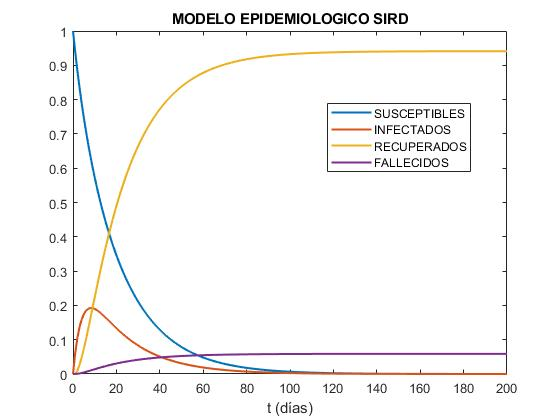
\includegraphics[width=0.8\textwidth]{Pictures/DIAG_EPIDEM.jpg}
 \end{figure}

\bigskip

Si se desea saber la evolución de la cantidad de individuos en cada estado después de 6 meses, se debe calcular $A^{180}$ !! 

Si $A$ fuera diagonal esto llevaría un  bajo costo computacional ya que quedarían elevados al exponente $180$  los elementos de la diagonal.



\bigskip

El prograna en lenguaje de programación GNU Octave que sigue diagonaliza la matriz $A$ del modelo. 
%Se sugiere al lector ejecutar  el programa  y comparar los tiempos de ejecución  para calcular $XF$ con la matriz $A$ y $XFD$ con la diagonalización.


\bigskip

% MODELO SIRD
% El 94% de la población sigue siendo susceptible. 6% adquiere la
% enfermedad
% El 1% morirá por la enfermedad, el 16% se recuperará y tendrá inmunidad. 
% El 3% se recuperará y no tendrá inmunidad, volverá a ser
% susceptible. El 80% seguirá infectado
% Los recuperados y los fallecidos permanecen en ese estado


\begin{lstlisting}[frame=single]
% MODELO SIRD 
%(SUSCEPTIBLES, INFECTADOS, RECUPERADOS, FALLECIDOS)
clear all
close all
A=[.94 .03 0 0 ; 0.06 .8 0 0 ; 0 0.16 1 0 ; 0 0.01 0 1];
X=[1 0 0 0 ]';
t=0:200;
for k= 1:200
    X(:,k+1)=A*X(:,k);
end
for k=1:4
%plot(t,X(k,:),'linewidth',1.5)
hold on
axis tight
end
XF=A^180
[U,D]=eig(A);
XFD=U*D^180*inv(U)
\end{lstlisting}

%[ht!]
\bigskip


\begin{remark}
Este ejemplo estuvo inspirado en la pandemia del COVID-19 del año 2020 y en estudios realizados en el tema, como el del trabajo \cite{covid}.  Los modelos matemáticos de epidemia que se utilizaron para su análisis  y para hacer predicciones  son modelos  de última generación,  representados mediante un sistema de ecuaciones diferenciales  con muchas variables y  poblaciones y que, entre otros  parámetros,  contemplan los que miden el comportamiento social. 
\end{remark}



En  la Sección \ref{cbaseTL} vimos, en el  Ejemplo \ref{ejemplo217}, que dada una aplicación lineal $T$ cuya matriz en la base canónica es 

$$T=\left(\begin{array}{cc}  6 & -2  \\ 6 &  -1
\end{array}
 \right)$$

\bigskip

\noindent
es posible hallar  una base tal que la matriz sea diagonal. 


$$T^\prime=\left(\begin{array}{cc}  2 & 0  \\ 0 &  3
\end{array}
\right)$$

\bigskip


La matriz $T^\prime$ en esa nueva base es mucho más sencilla que la matriz $T$ y se tiene que $T^\prime=C^{-1}TC$  donde $C$ es la matriz de cambio de base.
Nos surge  la pregunta si esto siempre es posible.


\bigskip


Un ejemplo sencillo que nos permite responder que no siempre es posible es la matriz 

$$T=\left(\begin{array}{cc}  1 & 1  \\ 0 &  1
\end{array}
 \right)$$

\bigskip


Supongamos existe una matriz $C$ de cambio de base  tal que 

\bigskip

$$C^{-1}TC=T^\prime=\left(\begin{array}{cc}  \alpha & 0  \\ 0 &  \beta
\end{array}
 \right)$$
 
\bigskip
\noindent
o en forma equivalente,

$$T=C\left(\begin{array}{cc}  \alpha & 0  \\ 0 &  \beta
\end{array}
 \right)C^{-1}$$ 
%ver H pag 284


\bigskip

$$\left(\begin{array}{cc}  1 & 1  \\ 0 &  1
\end{array}
 \right)= \left(\begin{array}{cc}  a & b  \\ c &  d
\end{array}
 \right) \left(\begin{array}{cc}  \alpha & 0  \\0 &  \beta
\end{array}
 \right) \left(\begin{array}{cc}  d & -b  \\ -c &  a
\end{array}
 \right) \frac{1} {Det(C)}$$

\bigskip

$$\left(\begin{array}{cc}  1 & 1  \\ 0 &  1
\end{array}
 \right)= \left(\begin{array}{cc}  a\alpha & b\beta  \\ c\alpha &  d\beta
\end{array}
 \right)  \left(\begin{array}{cc}  d & -b  \\ -c &  a
\end{array}
 \right) \frac{1} {Det(C)}$$
 
\bigskip 


$$\left(\begin{array}{cc}  1 & 1  \\ 0 &  1
\end{array}
 \right)= \left(\begin{array}{cc}  a\alpha d - b\beta c & -a\alpha b + b  \beta a \\ c \alpha d - c d \beta &  -c \alpha b +  d \beta a
\end{array}
 \right)   \frac{1} {Det(C)}$$

\bigskip

Igualando los elementos de ambas matrices, se tiene un sistema de ecuaciones:

\bigskip
\begin{eqnarray}
Det(C)&=& a\alpha d - b\beta c \\
Det(C)&=& ba( -\alpha  +   \beta )  \\
0&=&cd( -\alpha  +   \beta )  \\
Det(C)&=& -c \alpha b + d \beta a
\end{eqnarray}
 


\bigskip

\bigskip

De la igualdad $(3$.$3)$  se tiene que $c=0$ o $d=0$ o $\alpha = \beta$. Si $c=0$, de $(3$.$1)$ y ($3$.$4$), queda $Det(C)= a\alpha d= d \beta a$, de donde $\alpha = \beta$ y en $(3$.$3)$ se tiene $1=0$.
Si $d=0$, de $(3$.$1)$ y $3$.$4$,  $Det(C)= - b \beta c = -c\alpha b $, de donde también resulta $\alpha = \beta$ y en $(3.3)$ se tiene $1=0$. Lo mismo si $\alpha = \beta$. 

Se llega a una contradicción. Concluimos que no siempre es posible diagonalizar una matriz.

\bigskip

\begin{remark}
 \begin{itemize}
     \item 
No todas las matrices son diagonalizables.

\item 
Si es digonalizable,  $A$ es semejante a una matriz diagonal y tendremos ventaja al calcular su potencia. En otros casos  será semejante a una matriz casi diagonal.
  \item 
  Siempre es posible encontrar una forma \textit{ más sencilla} de una matriz dada  mediante un cambio de base. Se denomina \textit{matriz de Jordan de la matriz dada} y el nombre se debe al matemático Camille Jordan (1838-1922).
 \end{itemize}   
\end{remark}


\bigskip
Si se desea  calcular 

\bigskip

$$T^6=\left(\begin{array}{cc}  6 & -2  \\ 6 &  -1
\end{array}
 \right)^6$$

\bigskip
\noindent
como  $T=CT^\prime C^{-1}$,  $T^2=CT^\prime C^{-1} CT^\prime C^{-1}=CT^\prime I T^\prime C^{-1}=C(T^\prime)^2 C^{-1}$, y en general, 
$$T^n=C(T^\prime)^n C^{-1}, \quad n \in \mathbb{Z}$$
\noindent
de donde se tiene que 

\bigskip

$$T^6=\left(\begin{array}{cc}  1 & 2  \\ 2 &  3
\end{array}
 \right) \left(\begin{array}{cc}  2^6 & 0  \\ 0 &  3^6
\end{array}
 \right) \left(\begin{array}{cc}  -3 & 2  \\ 2 &  -1
\end{array}
 \right) $$

\bigskip

\section{Subespacios invariantes. Valores y vectores propios.}\index{Subespacios invariantes}
\label{Subespacios invariantes}


Dado un espacio vectorial $V$ y una aplicación lineal  $T: V \rightarrow V$, es decir $T \in L(V)$, un subespacio vectorial $W$ de $V$ se dice  \textit{invariante}   respecto a $T$ si $T(W)\subset W$, es decir si la imagen $T(\vec{x})$ de todo vector  $\vec{x}\in W$ es un elemento de $W$.

\bigskip

 %(es inyectiva si y sólo si  $N(T)=
\begin{example}

Sea $T\in L(\mathbb{R}^2)$ una aplicación lineal en $\mathbb{R}^2$ cuya matriz respecto de la base canónica $\left\{\vec{e_1} , \vec{e_2}\right\}$ de $\mathbb{R}^2$ está dada por 


$$T=\left(\begin{array}{cc}  2 & 0  \\ 0 &  1
\end{array}
\right)$$

\bigskip

Entonces $W_1=\left\{x_1\vec{e_1} ,~ x_1\in \mathbb{R}\right\}$ y $W_2=\left\{x_2\vec{e_2} ,~ x_2\in \mathbb{R}\right\}$ son invariantes respecto de $T$. 


\bigskip

En efecto, de la definición de matriz de una transformación lineal se tiene que $T(\vec{e_1})=2 \vec{e_1} + 0 \vec{e_2}$ y $T(\vec{e_2})=0 \vec{e_1} + 1 \vec{e_2}$.

\bigskip
Luego, 

$$T(x_1\vec{e_1})=x_1T(\vec{e_1})=x_1(2\vec{e_1})=(2x_1)\vec{e_1}\in W_1$$

y

$$T(x_2\vec{e_2})=x_2T(\vec{e_2})=x_2\vec{e_2}\in W_2$$

\end{example}
\bigskip

 %(es inyectiva si y sólo si  $N(T)=
\begin{example}

Sea $R_\alpha$ una rotación de ángulo $\alpha\neq 0$ en $\mathbb{R}^3$ con respecto al eje $z$. Geométricamente se observa que el plano $xy$ y el eje $z$ son invariantes con respecto a esta aplicación. Para comprobar algebraicamente que el plano $xy$ es invariante se observa, en primer lugar,  que la matriz de $R_\alpha$ con respecto a la base canónica de $\mathbb{R}^3$ es 


$$R=\left(\begin{array}{ccc} cos\alpha & -sen\alpha &  0 \\ sen\alpha & cos\alpha & 0
\\ 0 & 0 & 1
\end{array}
 \right).$$

\vskip0.25cm
Si $\vec{x}=x_1\vec{e_1}+ x_2\vec{e_2}$ es un elemento del plano $xy$, se tiene que su rotación da el vector



$$\left(\begin{array}{ccc} cos\alpha & -sen\alpha &  0 \\ sen\alpha & cos\alpha & 0
\\ 0 & 0 & 1
\end{array}
 \right)  \left(\begin{array}{c} x_1 \\ x_2
\\ 0 
\end{array}
 \right) =  \left(\begin{array}{c} x_1cos\alpha- x_2sen\alpha  \\ x_1sen\alpha+ x_2cos\alpha 
\\ 0 
\end{array}
 \right)   $$

 \bigskip
\noindent 
y, por lo tanto, $R_\alpha(\vec{x})= (x_1cos\alpha- x_2sen\alpha)\vec{e_1}+  (x_1sen\alpha+ x_2cos\alpha) \vec{e_2}     $  y  es nuevamente un elemento del plano $xy$.

\end{example}
\begin{figure}[ht]
    \centering
    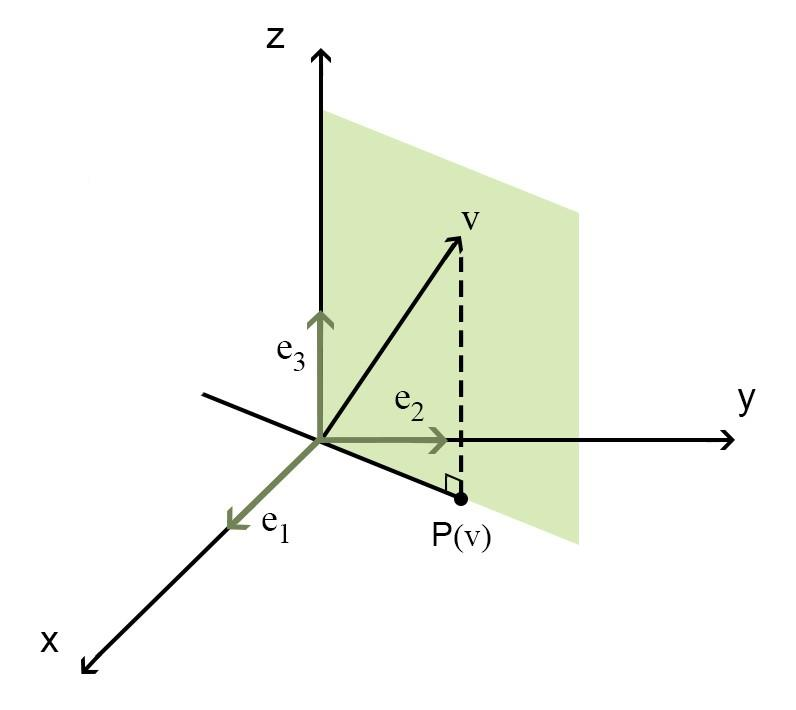
\includegraphics[width=0.70\textwidth]{Pictures/fig.35.jpg}
    \caption{Todo plano que contiene al eje $z$ es invariante por $P$.
    }
    \label{pag286}
\end{figure}

\bigskip

\begin{example}

En la Figura \ref{pag286} se muestra   la proyección ortogonal $P$ de $\mathbb{R}^3$  sobre el plano $xy$. (Ver Ejemplo \ref{proyxy}). La matriz de $P$ es 
$$P=\left(\begin{array}{ccc} 1 & 0 &  0 \\ 0 & 1 & 0
\\ 0 & 0 & 0
\end{array}
 \right)$$
con respecto a la base canónica. Se puede ver que todo plano $\pi$  que contiene al eje $z$ es invariante:

\noindent
el plano  $\pi$ tiene ecuación $x_1 x +  x_2 y + x_3 z=0$, donde $x_3=0$ ya que $(0,0,1) \in \pi$. Los vectores de ese plano  son de la forma
$\vec{x}=x_1\vec{e_1} + \lambda x_1\vec{e_2} + x_3\vec{e_3}, ~\lambda \in \mathbb{R}$,
y se  tiene que su imagen, $P(\vec{x})$,  es de nuevo un elemento del plano $\pi$:
$$P=\left(\begin{array}{ccc} 1 & 0 &  0 \\ 0 & 1 & 0
\\ 0 & 0 & 0
\end{array}
 \right)      \left(\begin{array}{c} x_1 \\ \lambda x_1
\\ x_3
\end{array}
 \right) =   \left(\begin{array}{c} x_1 \\ \lambda x_1
\\ 0
\end{array}
 \right)            $$



\bigskip
% agregar figura de la pág. 286 VH




Otros subespacios invariantes de esta proyección ortogonal son el plano $xy$, el eje $z$ y cualquier recta del plano $xy$ que pase por el origen de coordenadas.
\end{example}

\bigskip

\begin{remark}
Para cualquier transformación lineal  $T\in L(V)$ ( o endomorfismo), el subespacio $S=\left\{\vec{0}\right\}$, formado sólo por el elemento nulo, es invariante ya que $T(\vec{0})=\vec{0}$ y el propio espacio vectorial $V$ es también invariante ya que $T(\vec{x})$ para todo vector  $\vec{x}\in V$ es un elemento de $V$.
%\hfill$\blacktriangle$
\end{remark}

\bigskip

\begin{theorem}
\label{intysumainv}
\noindent
La intersección y la suma de subespacios invariantes respecto de una aplicación lineal $T\in L(V)$ son subespacios invariantes respecto de $T$.

%\begin{proof}
Se deja la demostración al lector.
%\end{proof}

\end{theorem} 

\bigskip

\bigskip

\bigskip


\begin{definition}\index{Autovector (o vector propio)}\index{Autovalor (o valor propio)}
%\label{eigen}

\bigskip

Un vector $\vec{v}\neq \vec{0}$ de un espacio vectorial $V$ sobre $K$ se llama \textit{autovector} o \textit{vector propio}  de una aplicación lineal $T\in L(V)$ si existe un escalar $\lambda \in K$ tal que $T(\vec{v})=\lambda \vec{v}$. Este número $\lambda $ se denomina \textit{autovalor }o \textit{valor propio} de la aplicación $T$ correspondiente al vector $\vec{v}$.

\end{definition}

\bigskip

\begin{remark}
Si $\vec{v}$  es un vector propio de $T$ con autovalor  $\lambda$, todo elemento no nulo del subespacio unidimensional generado por $\vec{v}$ es un autovector de $T$ con el mismo autovalor $\lambda $. Esto es porque $T(c \vec{v})=c T(\vec{v})= c \lambda \vec{v}=\lambda (c\vec{v}) $.
%\hfill$\blacktriangle$
\end{remark}
\bigskip



\begin{figure}
    \centering
    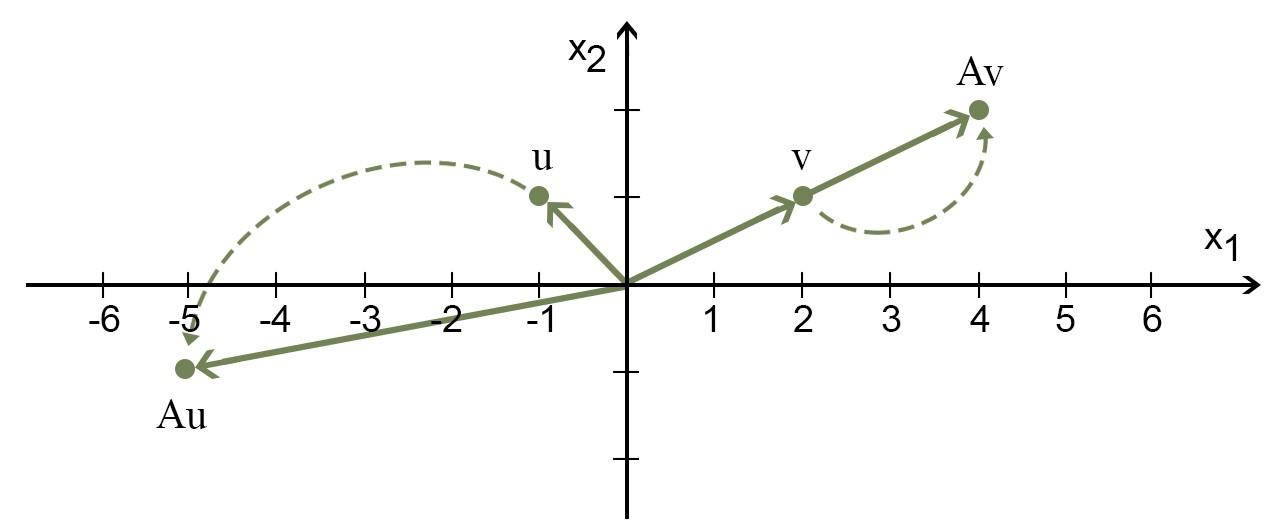
\includegraphics[width=0.90\textwidth]{Pictures/FIGAuAv.jpg}
    \caption{El vector $\vec{v}$ es autovector de $A$, mientras que el vector $\vec{u}$ no es autovector,   $A\vec{u}$  no es múltiplo de $\vec{u}$.}
    \label{FIGAuAv}
\end{figure}

\bigskip

\begin{theorem}
\label{PROPOSICION3}
Una aplicación lineal  $T\in L(V)$ es diagonalizable sí y sólo sí existe una base de $V$ formada por vectores propios.

\begin{proof}

Supongamos que una aplicación lineal $T$ en un espacio $V$ de dimensión $n$ tiene $n$ vectores propios linealmente independientes, $\vec{e}_1,\vec{e}_2, \cdots ,\vec{e}_n$ con valores propios $\lambda_1,\lambda_2, \cdots ,\lambda_n$ respectivamente, tomando $\left\{\vec{e}_1,\vec{e}_2, \cdots,\vec{e}_n\right\}$ como una base de $V$ se tiene que 

$$T(\vec{e}_1)=\lambda_1\vec{e}_1, T(\vec{e}_2)=\lambda_2\vec{e}_2, \cdots,T(\vec{e}_n)=\lambda_n\vec{e}_n$$

\bigskip

\noindent
y, por lo tanto, la matriz de $T$ con respecto a esta base es la matriz diagonal

\bigskip


$$T=\left(\begin{array}{ccccc} \lambda_1 & 0 &  0 & 0 &  0\\ 0 &  \lambda_2 & 0  & 0 & 0
\\ 0 & 0  &\ddots   &  0 &   0  \\   0 & 0 &  0 &\ddots   &  0   \\ 0 & 0 & 0 & 0 & \lambda_n
\end{array}
 \right)$$



\bigskip


Recíprocamente, toda aplicación lineal que tiene una matriz diagonal en una cierta base, tiene a los elementos de esta base como vectores propios. 


\bigskip


\end{proof}

\end{theorem}

\bigskip

\begin{remark}
Una aplicación lineal  $T\in L(V)$ es \textit{diagonalizable} sí y solo sí existe una base de $V$ en la cual la matriz de $T$ es diagonal.
%\hfill$\blacktriangle$
\end{remark}


\begin{definition}\label{Diag}\index{Matriz diagonalizable}

Una matriz $T\in K^{n \times n}$ se dice diagonalizable en $K$ si la aplicación lineal  $T: K^n \rightarrow  K^n$ que la matriz que la representa es diagonalizable.

\end{definition}

\bigskip
\noindent
De esta definición se deduce que una matriz es diagonalizable en $K$ si existe una matriz $C\in K^{n \times n}$ con determinante no nulo, tal que $T^\prime=C^{-1}TC$ es una matriz diagonal.

\bigskip





\noindent
En el ejemplo del inicio de la sección, para 

$$T=\left(\begin{array}{cc}  6 & -2  \\ 6 &  -1
\end{array}
 \right)$$
 \noindent
se tiene que 
 
 
$$\left(\begin{array}{cc}  6 & -2  \\ 6 &  -1
\end{array}
 \right) \left(\begin{array}{c}  1   \\ 2 
\end{array}
 \right) = \left(\begin{array}{c}  2  \\ 4 
\end{array}
 \right)  = 2 \left(\begin{array}{c}  1  \\ 2 
\end{array}
 \right)  $$
 
\bigskip

$$\left(\begin{array}{cc}  6 & -2  \\ 6 &  -1
\end{array}
 \right) \left(\begin{array}{c}  2   \\  3
\end{array}
 \right) = \left(\begin{array}{c}  6  \\ 9 
\end{array}
 \right)  = 3 \left(\begin{array}{c}  2  \\ 3 
\end{array}
 \right)  $$

\bigskip

Se tiene que $T(\vec{v}_1)=  2 \vec{v}_1$ y  $T(\vec{v}_2)=  3 \vec{v}_2$, siendo    $\vec{v}_1=(1, 2)$ y $\vec{v}_2=(2, 3)$, con lo que $\vec{v}_1 $ y $ \vec{v}_2$ son vectores propios de $T$ con sus correspondientes valores propios $2$ y $3$ respectivamente.
Como $\vec{v}_1$ y $\vec{v}_2$  forman una base de $\mathbb{R}^2$ (son linealmente independientes y son $2$), la matriz $T$ es diagonalizable en $\mathbb{R}$ y su matriz diagonal asociada es 

$$\left(\begin{array}{cc}  2 & 0  \\ 0 &  3
\end{array}
 \right)$$
 
\bigskip


\noindent
\textbf{Cálculo de  autovalores y autovectores de una transformación lineal.}

\bigskip

Supongamos que $\vec{v}$ es un vector propio de una aplicación lineal $T$ en un espacio vectorial $V$ y que $\lambda$ es su autovalor, es decir $T(\vec{v})=\lambda \vec{v}$. Sea $\left\{\vec{e}_1,\vec{e}_2, \cdots,\vec{e}_n\right\}$ una base de $V$ y  sean   $v_{j}$, $ j=1,\cdots n $ las coordenadas de  $\vec{v}$ en esa base, es decir,  $\vec{v}=\sum_{j=1}^{n}v_{j}\vec{e}_j$. Si $(a_{ij})$ es la matriz 
de $T$ con respecto a la base tenemos que 


$$\sum_{j=1}^{n} \lambda v_{j}\vec{e}_j = \lambda \sum_{j=1}^{n}  v_{j}\vec{e}_j = \lambda \vec{v}=T(\vec{v})=T(\sum_{j=1}^{n}  v_{j}\vec{e}_j) $$

%\newpage

\bigskip


$$ =\sum_{j=1}^{n}  v_{j} T(\vec{e}_j )= \sum_{j=1}^{n}  v_{j}  (\sum_{i=1}^{n}  a_{ij}\vec{e}_i)=  \sum_{i=1}^{n}   (\sum_{j=1}^{n}  a_{ij} v_{j})\vec{e}_i $$

\bigskip

Como $\left\{\vec{e}_1,\vec{e}_2, \cdots,\vec{e}_n\right\}$ es una base de $V$, del primer y del último término de la igualdad anterior se tiene que: 

\bigskip

\begin{equation} \label{matriz A0}
\left\{ \begin{array} {ccl} 
                    \lambda v_1&=&a_{11}v_1+a_{12}v_2+\cdots +a_{1n}v_n    \\
                    \lambda v_2&=&a_{21}v_1+a_{22}v_2+\cdots +a_{2n}v_n  \\
										\cdots  \\
                    \lambda v_n&=&a_{n1}v_1+a_{n2}v_2+\cdots +a_{nn}v_n  
                   \end{array}
           \right.
\end{equation}

\bigskip

\noindent
o en forma equivalente,

\bigskip

\begin{equation} \label{matriz A}
\left\{ \begin{array} {ccl} 
                    (a_{11}-\lambda)v_1+a_{12}v_2+\cdots +a_{1n}v_n  =& 0  \\
                    a_{21}v_1+(a_{22}-\lambda)v_2+\cdots +a_{2n}v_n =& 0 \\
										\cdots  \\
                    a_{n1}v_1+a_{n2}v_2+\cdots +(a_{nn}-\lambda)v_n  =& 0
                   \end{array}
           \right.
\end{equation}

\bigskip


Como es un sistema homogéneo, para que exista una solución no nula debe ocurrir que 

\bigskip

\begin{equation} \label{polca}
Det(A-\lambda I)=\left(\begin{array}{cccccc}a_{11}-\lambda & a_{12} & a_{13} &\cdots  &\cdots & a_{1n}\\ a_{21} & a_{22}-\lambda    &\cdots  &\cdots  &\cdots &a_{2n}
\\\cdots & \cdots   &\ddots   &  \cdots  &   \cdots   \\ \cdots & \cdots  & \cdots  &  \ddots  &\cdots   & \cdots  
\\ \cdots & \cdots  & \cdots  &  \cdots  &\ddots   & \cdots 
\\ a_{n1} & a_{n2}  &  &\cdots  &  a_{nn-1} & a_{nn}-\lambda
\end{array}
 \right) =  0
\end{equation}

\bigskip

\noindent
donde $I$ denota la matriz identidad. Esto es una ecuación de grado $n$ en $\lambda$ y sus soluciones en $K$ ($\mathbb{R}$ o $\mathbb{C}$) son los autovalores de $T$. 
Si $V$ es un espacio vectorial complejo, por el teorema fundamental del álgebra la ecuación anterior tiene $n$ soluciones complejas contando cada una con su multiplicidad. Si $V$ es un espacio vectorial real, no podemos asegurar que la ecuación anterior tenga $n$ soluciones reales.


\bigskip
%En base a lo anterior, los 
{\textbf{Pasos para resolver $A\vec{v}=\lambda \vec{v}$}}

\bigskip

\begin{enumerate}
\item
Se calcula $ Det(A-\lambda I)$ (se anota en forma equivalente como $\left   | A -  \lambda I   \right  |$)      , restando $ \lambda $ de los elementos de la diagonal de la matriz $A$. Es un polinomio de grado $n$, con coeficiente $ (-\lambda)^n $. 

\bigskip

\item
Se hallan las raíces de este polinomio. Las $n$ raíces son los autovalores de la matriz $A$.

\bigskip

\item
Para cada autovalor $ \lambda $, se resuelve el sistema lineal  $(A-\lambda I) \vec{v}=   \vec{0} $. Como el determinante es cero, tendrá soluciones no nulas. Esos son los autovectores.


\end{enumerate}


\bigskip

\bigskip

\begin{example}
\label{ejemploaut}
\noindent
Se desea determinar los valores y vectores propios de la aplicación lineal de $T: V \rightarrow V$, $V=\mathbb{R}^2$, que tiene como matriz, 

\bigskip

$$T=\left(\begin{array}{cc}  1 & 2  \\ 5 &  4
\end{array}
 \right)$$

\begin{enumerate}
\item
\[
0= 
\left   | T -  \lambda I   \right  |=\left | \begin{array}{cc}
1- \lambda  & 2  \\
5 &  4- \lambda 
\end{array}
\right|=(1- \lambda)(4- \lambda)-10= \lambda^2 - 5 \lambda -6
\]


\bigskip

\item
Las raíces son $\lambda_1= 6$ y $\lambda_2=-1$

\bigskip


\item

Para $\lambda_1= 6$  se resuelve el sistema 

$$(T-6I) \left(\begin{array}{c}  x_1  \\ x_2 
\end{array}
 \right)=  \left(\begin{array}{c}  0  \\ 0 
\end{array}
 \right) $$

 Los vectores propios correspondientes a $\lambda_1= 6$  son de la forma $ \alpha  \left(\begin{array}{c}  2  \\ 5 
\end{array}
 \right)$.

\bigskip

 
Para $\lambda_2= -1$  se resuelve el sistema 

$$(T-(-1)I) \left(\begin{array}{c}  x_1  \\ x_2 
\end{array}
 \right)=  \left(\begin{array}{c}  0  \\ 0 
\end{array}
 \right) $$

 Los vectores propios correspondientes a $\lambda_2= 6$  son de la forma $ \beta  \left(\begin{array}{c}  1  \\ -1 
\end{array}
 \right)$.
 \end{enumerate}
 
\bigskip


 Como $  \left(\begin{array}{c}  2  \\ 5 
\end{array}
 \right)$  y $  \left(\begin{array}{c}  1  \\ -1 
\end{array}
 \right)$  forman una base de $\mathbb{R}^2$, por la Proposición \ref{PROPOSICION3},  $T$ es diagonalizable, 
 
 \bigskip

 \bigskip
 
 \noindent
 con matriz diagonal 

 $$\left(\begin{array}{cc}  6 & 0  \\ 0 &  -1
\end{array}
 \right)$$
 
 \bigskip

 
\noindent
 y la matriz de  cambio de base (de la base de autovectores a la base canónica) está dada por la matriz

 $$C=\left(\begin{array}{cc}  2 & 1  \\ 5 &  -1
\end{array}
 \right)$$
\end{example}


\bigskip
\index{Strang, William Gilbert}
\begin{parchment}[William Gilbert Strang  (1934)] {Es un matemático estadounidense, actualmente Professor Mathworks de Matemáticas del Department of Mathematics del Massachusetts Institute of Technology (MIT). Ha contribuido a la teoría de elementos finitos, al cálculo de variaciones, al análisis wavelet y al  álgebra lineal. Ha contribuido enormemente a la educación en matemáticas, en forma de libros técnicos y cursos online. En MIT enseña Álgebra Lineal, Ciencia Computacional e Ingeniería, Aprendiendo de los Datos. Sus clases están disponibles en la plataforma MIT OpenCourseWare (en inglés).
Gilbert Strang nació en Chicago, Illinois. Cursó estudios en el propio MIT y en el Balliol College, en la Universidad de Oxford. Se doctoró en la Universidad de California, Los Ángeles (UCLA) y desde ese momento ha llevado a cabo su actividad docente en el MIT. Entre las publicaciones más notables del Professor Strang se destaca An Analysis of the Finite Element Method, conjuntamente con George Fix, así como seis manuales:
Introduction to Linear Algebra (1993, 1998, 2003),
Linear Algebra and Its Applications (1976, 1980, 1988, 2005),
Introduction to Applied Mathematics (1986),
Calculus (1991),
Wavelets and Filter Banks, con Truong Nguyen (1996),
Linear Algebra, Geodesy, and GPS, con Kai Borre (1997).

Gilbert Strang fue Presidente de la SIAM (Society for Industrial and Applied Mathematics) durante los años 1999-2000. También ha sido Chairman of the US National Committee on Mathematics durante los años 2003-2004. Es Honorary Fellow, en el Balliol College de Oxford. También es Chairman, en la National Science Foundation (NSF) del Advisory Panel del área de Matemáticas.

Fue pionero al abrir sus clases y permitir que fueran grabadas en vídeo mientras explicaba matemáticas a sus alumnos del MIT para su difusión abierta y gratuita en Internet. \cite{gstrang}}
\end{parchment}


%\newpage

\bigskip

%Completar del hernández pág 290


\subsection{Localización de autovalores}\index{Localización de autovalores}

\bigskip

\begin{corollary}
\label{Teodiscos}
Teorema de Gershgorin. \index{Gershgorin}

Los autovalores de una matriz $A$ están en la unión de los discos $D_1$, $D_2$, $\cdots$, $D_n$ (del plano complejo) donde $D_i$ es el disco centrado en el elemento de la diagonal $a_{ii}$: 

$$|\lambda-a_{ii}|  \leq  r_i  $$

Su radio $r_i=\sum_{j \neq i} |a_{ij}|$ es igual a la suma de los valores absolutos de los elementos del resto de la fila.


\begin{proof}
Supongamos $v_i$ es la mayor componente en valor absoluto del autovector  $\vec{v}$,  $ A\vec{v}=\lambda \vec{v}$. Entonces,

\bigskip

$(\lambda-a_{ii})v_i= \sum_{j \neq i} a_{ij} v_j$, de donde, 

\bigskip

$|\lambda-a_{ii}|  \leq  \sum_{j \neq i} |a_{ij}| \frac{   |v_j|}{ |v_i| } \leq  \sum_{j \neq i} |a_{ij}|=r_i  $

\end{proof}
\end{corollary}

\bigskip


\begin{example}
Dada la matriz,

\bigskip

$$A=\left(\begin{array}{cccc} 3 & 0 &  -1 & 1/2 \\ 0 & 5   & 1/2 & 1
\\  -1/2  &  0 &  -3 &   5/4

\\   0 & 1/2 &  1/2 & 4 
\end{array}
 \right)$$

 \bigskip

 
Se muestra en la Figura \ref{DISCOS} la localización de sus autovalores de acuerdo al Teorema \ref{Teodiscos}. Los discos están centrados en los elementos de la diagonal de la matriz $A$ y tienen radios $r_1=3/2$, $r_2=3/2$, $r_3=7/4$ y $r_4=1$. Están en el intervalo $[-19/4,7]$, en el caso que sean números reales.

 \bigskip
 
\begin{figure}
    \centering
    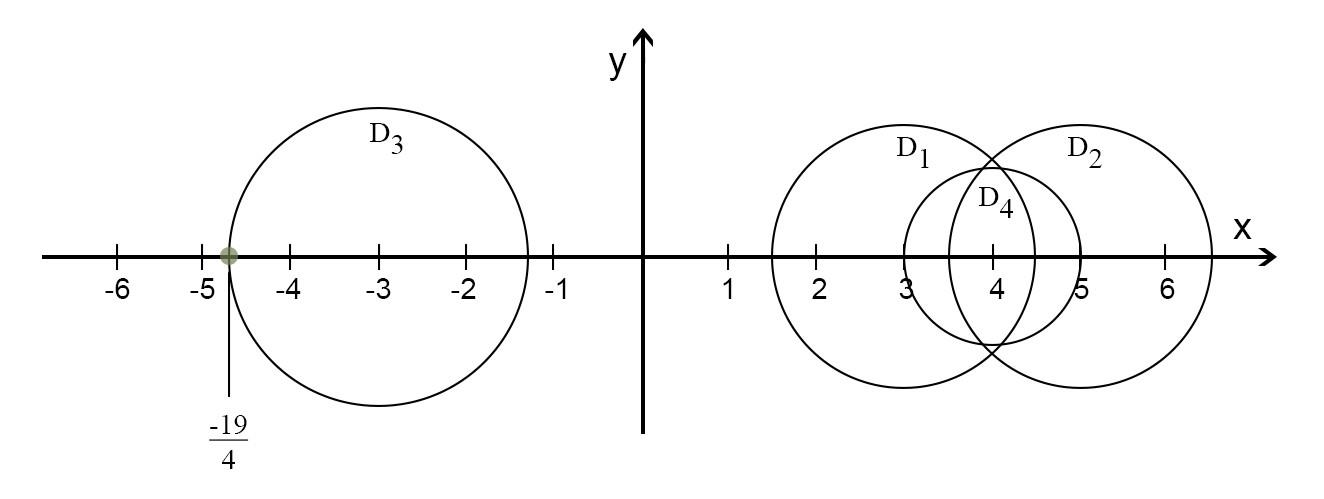
\includegraphics[width=0.90\textwidth]{Pictures/DISCOS.jpg}
    \caption{Los autovalores de $A$ se encuentran en la unión de los cuatro discos, $D_1, D_2, D_3$ y $D_4$.}
    \label{DISCOS}
\end{figure}


\end{example}
\bigskip

Para la matriz del Ejemplo \ref{ejemploaut} se  tienen los discos  $D_1=|\lambda-1|  \leq 2$ y $D_2=|\lambda-4|  \leq 5$.  Sin calcular los autovalores, se sabe que si son números reales, estarán  en el intervalo $[-1,9]$.


\section{Polinomio característico}
\label{polcar}

Al polinomio $Det(T-\lambda I) \in P_K^{(n)}\left[\lambda\right]$  (Ec. (\ref{polca})) se lo denomina \textit{polinomio característico} de la aplicación $T$  (o de la matriz $A \in K^{n \times n}$). Lo anotaremos  $\mathbf{P}_T( \lambda) $.

\bigskip

\begin{theorem}
\label{proppolauto}

Sea $T\in K^{n \times n}$ y sea $\lambda \in K$. Entonces $\lambda$ es autovalor de $T$ sí y sólo sí $\lambda$ es raíz del polinomio característico de $T$.


\end{theorem}

\bigskip

\begin{example}
La matriz 
$$\left(\begin{array}{cc}  0 & 1  \\ -1 &  0
\end{array}
 \right)$$

 \bigskip
\noindent 
es diagonalizable en $\mathbb{C}^{n \times n}$, pero no es diagonalizable en $\mathbb{Q}^{n \times n}$ ni en $\mathbb{R}^{n \times n}$. Sus autovalores son las raíces del polinomio


$$Det\left(\begin{array}{cc}  0-\lambda  & 1  \\ -1 &  0-\lambda
\end{array}
 \right)= \lambda^2+1=0 $$

\bigskip

Se tiene, entonces, que los autovalores son $\lambda_{1-2}= \mp i$
%y no dependen de la base elegida.
\end{example}






\bigskip


\begin{theorem}
\label{polcarbase}
El polinomio característico no depende de la base elegida en $V$ para representar la aplicación lineal  $T$.


\begin{proof}


\noindent
Sea $\mathbf{P}_{T,B}(\lambda)=Det(T-\lambda I)$ el polinomio característico  de la aplicación $T$ en la base $B=\left\{\vec{e}_1,\vec{e}_2, \cdots,\vec{e}_n\right\}$  de $V$ y sea  $\mathbf{P}_{T,B^{\prime}}(\lambda)=Det(T^{\prime}-\lambda I)$ el polinomio característico de $T$ en la base $B^{\prime} =\left\{\vec{e ^{\prime}}_1,\vec{ e ^{\prime}}_2,\cdots, \vec{e^{\prime}}_m\right\}$; si $C$ es la matriz del cambio de base, se  sabe que    $T=CT^\prime C^{-1}$, 
y se tiene 

\bigskip

$$\mathbf{P}_{T,B}(\lambda)=\mathbf{P}_{T,B^{\prime}}(\lambda)$$  

Se deja al lector  completar esta demostración.

\end{proof}
\end{theorem}

\bigskip

\bigskip

\begin{example}
La matriz de la proyección sobre el eje $x$, $ P_x$, (Ver Ejemplo \ref{proyejex}) en la base canónica $B=\{\vec{e}_1, \vec{e}_2 \}  $ es 

$$\left(\begin{array}{cc}  1 & 0  \\ 0 &  0
\end{array}
 \right)$$

 \bigskip
 
 Los autovalores son $\lambda_1=1$ y $\lambda_2=0$, ya que para los vectores $\vec{v}_1$ que están sobre el eje $x$ se verifica $P_x(\vec{v}_1)=1\vec{v}_1$, mientras que para los los vectores $\vec{v}_2$ que están sobre el eje $y$ se verifica $P_x(\vec{v}_2)=\Vec{0}$.
 
\bigskip
Si cambio de base, por ejemplo a la base $B^{\prime}= \{\vec{e}_1^{\prime}, \vec{e}_2^{\prime} \} $ (rotando  en $ \phi= \pi/4$ los vectores de la base canónica $B$),  donde los vectores de $B^{\prime}$ son las columnas de la matriz $A$ del Ejemplo \ref{ejrotR2}, se tendrá que 

$$ P_x( \vec{e}_1^{\prime})=(\sqrt 2/2,0)= 1/2 \vec{e}_1^{\prime} -1/2 \vec{e}_2^{\prime} $$
y 

$$ P_x( \vec{e}_2^{\prime})=(-\sqrt 2 /2,0)= -1/2 \vec{e}_1^{\prime} +1/2 \vec{e}_2^{\prime} $$

\noindent
entonces la matriz en esta nueva base es

$$\left(\begin{array}{cc}  1/2 & -1/2  \\ -1/2 &  1/2
\end{array}
 \right)$$

 \bigskip

 Ahora el polinomio característico es $\mathbf{P}_{P_x,B^{\prime}}(\lambda)(1/2-\lambda)^2 -1/4$, con las mismas raíces, $\lambda_1=1$ y $\lambda_2=0$, y los mismos autovectores que se obtuvieron con la base $B$, ya que

 \bigskip
 
 $\vec{v}^{\prime}_1= (1,-1)_{B^{\prime}}= 1(\sqrt 2 /2,\sqrt 2 /2)-1(-\sqrt 2 /2,\sqrt 2 /2)=(1,0)$ y
 
 \bigskip
 
 $\vec{v}^{\prime}_2= (1,1)_{B^{\prime}}=1(\sqrt 2 /2,\sqrt 2 /2)+1(-\sqrt 2 /2,\sqrt 2 /2)=(0,1)$.

 \bigskip
 
 Se verifica, entonces, como se vió en la  Observación 
 \textcolor{blue}{{\fontfamily{qcr}\selectfont{i}}} en  \ref{Obssemejanza} que las matrices de una misma transformación lineal en distintas bases son semejantes.  
Se tiene la relación, 

\bigskip

$$\left(\begin{array}{cc}  1 & 0  \\ 0 &  0
\end{array}
 \right)=  P _{B,B^{\prime}} \left(\begin{array}{cc}  1/2 & -1/2  \\ -1/2 &  1/2
\end{array}
 \right)P _{B^{\prime},B}$$
 
\bigskip
 
\noindent
 donde $P _{B,B^{\prime}}$ y $P _{B^{\prime},B}$ son las matrices del cambio de base de $B^{\prime}$ a $B$ y de $B$ a 
 $B^{\prime}$, respectivamente.
  \end{example}
  
 \bigskip
 
\begin{example}
\label{rotautov}


Se quieren determinar los valores y vectores propios de la aplicación lineal que corresponde a la rotación de ángulo $\alpha$ que tiene como matriz: (ver la matriz \ref{matrizrotR2}, Ejemplo  \ref{ejrotR2} )

\bigskip



$$R_\alpha=\left(\begin{array}{cc}  cos(\alpha) &-sen(\alpha)  \\ sen(\alpha) & cos(\alpha)
\end{array}
 \right)$$
\noindent
con respecto a la base canónica de $\mathbb{R}^2$.



\[
0= 
\left   | R_\alpha -   \lambda I \right  | = \left|\begin{array}{cc}
 cos(\alpha)-\lambda  & -sen(\alpha) \\
sen(\alpha) &  cos(\alpha)- \lambda 
\end{array}
\right| \]
\[=(cos(\alpha)- \lambda)^2+ sen^2(\alpha)= \lambda^2 - 2 cos(\alpha )\lambda +1
\]

\bigskip

Las raíces son $\lambda_1= cos(\alpha) + i sen(\alpha)$ y $\lambda_2= cos(\alpha) - i sen(\alpha)$, que son números complejos a no ser que $ \alpha = 2k \pi $ o $ \alpha = (2k+1) \pi $, con $k \in \mathbb{Z}$.

\bigskip

Si $ \alpha = 2k \pi $, se tiene la matriz identidad  y todo vector de $\mathbb{R}^2$ es autovector, y corresponden a $ \lambda=1$. 

\bigskip

Mientras que si $ \alpha = (2k+1) \pi $, la matriz es $-I$ y también resulta autovector cualquier vector de $\mathbb{R}^2$, y corresponden a $ \lambda=-1$. En este caso la transformación es una simetría respecto al origen de coordenadas.
\end{example}

\bigskip

\begin{example}
\noindent
La matriz correspondiente a una rotación de ángulo $\alpha$ en $\mathbb{R}^3$ con respecto al eje $z$, es,

$$R=\left(\begin{array}{ccc} cos(\alpha) & -sen(\alpha) &  0 \\ sen(\alpha) & cos(\alpha) & 0
\\ 0 & 0 & 1
\end{array}
 \right)$$

\bigskip

 Su polinomio característico es $  (\lambda^2 - 2 (cos(\alpha) )\lambda +1)(1-\lambda)$, cuyas raíces  son $\lambda_1= cos(\alpha) + i sen(\alpha)$, $\lambda_2= cos(\alpha) - i sen(\alpha)$ y $ \lambda_3= 1$.


\bigskip

Los vectores propios correspondientes a  $ \lambda_3= 1$ son las soluciones del sistema:
 
 \begin{eqnarray}
 \label{sisr3rot}
\left(\begin{array}{ccc} cos(\alpha) -1 & -sen(\alpha) &  0 \\ sen(\alpha) & cos(\alpha)-1 & 0
\\ 0 & 0 & 1
\end{array}
 \right)  \left(\begin{array}{c} x_1\\ x_2
\\ x_3
\end{array}
 \right) =  \left(\begin{array}{c} 0\\ 0
\\ 0
\end{array}
 \right) 
\end{eqnarray} 

 \bigskip
 
 Dado que 
\[
 \left|\begin{array}{cc}
 cos(\alpha)-1  & -sen(\alpha) \\
sen(\alpha) &  cos(\alpha)- 1 
\end{array}
\right|\]
\[=(cos(\alpha)- 1)^2+ sen^2(\alpha)= 2 - 2 cos(\alpha) =  4 sen^2 (\alpha /2 )
\]
El sistema (\ref{sisr3rot}) tiene únicamente la solución $x_1=x_2=0 $  si $ \alpha \neq 2k \pi $, con $k \in  \mathbb{Z}$. En este caso los autovectores correspondientes a $\lambda_3= 1$, son los vectores sobre el eje $z$, de la forma $(0,0,x_3)$.

\bigskip

Si $ \alpha = 2k \pi $, se trata de la identidad y todos los vectores de $ \mathbb{R}^3$ son autovectores.

\bigskip

Si $ \alpha = (2k+1) \pi $, $ $ $\lambda_1=\lambda_2= -1$, y los autovectores son las soluciones del sistema 

\bigskip

$$\left(\begin{array}{ccc} 0 & 0&  0 \\ 0 & 0 & 0
\\ 0 & 0 & 2
\end{array}
 \right)  \left(\begin{array}{c} x_1\\ x_2
\\ x_3
\end{array}
 \right) =  \left(\begin{array}{c} 0\\ 0
\\ 0
\end{array}
 \right)$$
 
\bigskip
\noindent
y son los vectores  $ (x_1, x_2,0)$ o sea del plano $xy$, y la transformación es una simetría respecto al eje $z$.

\end{example}

\bigskip



\section{Diagonalización.}
\label{diago}

La Proposición \ref{PROPOSICION3} nos da una condición necesaria y suficiente para saber cuándo una aplicación lineal es diagonalizable, a saber, que exista una base del espacio vectorial $V$ formada por vectores propios. En algunos casos puede resultar laborioso encontrar esta base. Una condición que es suficiente para poder asegurar la diagonalizaciónde una matriz está contenida en la proposición siguiente:



\bigskip


\begin{theorem}

\label{PROPOSICION4}



Los vectores propios de una aplicación $T$ correspon-\ dientes a valores propios distintos dos a dos, son linealmente independien-\ tes.

\begin{proof}
%ver hojita 27
Por inducción sobre la cantidad de vectores. 
\begin{itemize}
\item

Para $k=2$.
Supongamos que  se tienen $\Vec{v}_1$ correspondiente a $ \lambda_1 $ y $\Vec{v}_2$ correspondiente a $ \lambda_2 $, con $ \lambda_1  \neq \lambda_2 $.  

Si se tiene
\begin{eqnarray}
\label{auton2li}
 \alpha_1 \Vec{v}_1 + \alpha_2 \Vec{v}_2 &= &\Vec{0} \\
 T(\alpha_1 \Vec{v}_1 + \alpha_2 \Vec{v}_2 )&=&T( \Vec{0})=\Vec{0} \nonumber\\
\alpha_1 T(\Vec{v}_1) + \alpha_1 T(\Vec{v}_2 )&=&\Vec{0} \nonumber\\
\alpha_1 \lambda_1\Vec{v}_1 + \alpha_1 \lambda_2\Vec{v}_2 &=&\Vec{0} \nonumber
\end{eqnarray}

\bigskip

 De (\ref{auton2li}) se tiene que  $  \alpha_2 \Vec{v}_2 = - \alpha_1 \Vec{v}_1$. Si se reemplaza en la última ecuación, se tiene que
\begin{eqnarray}
 \alpha_1 \lambda_1\Vec{v}_1 - \alpha_1 \lambda_2 \Vec{v}_1 &=&\Vec{0} \nonumber\\
 \alpha_1 \Vec{v}_1( \lambda_1 - \lambda_2) &=&\Vec{0} 
 \end{eqnarray}


\bigskip 

 Como $\Vec{v}_1 \neq \Vec{0}$ y $ \lambda_1 - \lambda_2 \neq  0$, resulta  $ \alpha_1=0$, de donde  $ \alpha_2=0$, pues
 $\Vec{v}_2 \neq \Vec{0}$.

 \bigskip 
 
 Por lo tanto, $\Vec{v}_1$ y $\Vec{v}_2$ son linealmente independientes.


  \bigskip 
  
\item

Supongamos ahora el resultado es válido para $k-1$ autovalores distintos.

Si 

$\alpha_1 \Vec{v}_1 + \alpha_2 \Vec{v}_2  + \cdots + \alpha_{k-1} \Vec{v}_{k-1} + \alpha_{k} \Vec{v}_{k} = \Vec{0},$

\bigskip

como en el caso $k=2$, aplicamos $T$, despejamos de la igualdad anterior el término $\alpha_{k} \Vec{v}_{k}$. 

Entonces,

\bigskip 

$ \alpha_1 \lambda_1\Vec{v}_1 + \alpha_2 \lambda_2\Vec{v}_2 + \cdots  +\alpha_{k-1} \lambda_{k-1}\Vec{v}_{k-1}+  \alpha_{k} \lambda_{k}\Vec{v}_{k}=  \Vec{0} $

\bigskip

$ \alpha_1 \lambda_1\Vec{v}_1 + \alpha_2 \lambda_2\Vec{v}_2 + \cdots  +\alpha_{k-1} \lambda_{k-1}\Vec{v}_{k-1}+( -\alpha_1 \Vec{v}_1 - \alpha_2 \Vec{v}_2  - \cdots - \alpha_{k-1} \Vec{v}_{k-1}) \lambda_k =  \Vec{0} $

\bigskip



$ \alpha_1( \lambda_1 - \lambda_k) \Vec{v}_1 + \alpha_2 (\lambda_2 - \lambda_k) \Vec{v}_2 + \cdots  +\alpha_{k-1} (\lambda_{k-1} - \lambda_k) \Vec{v}_{k-1}=  \Vec{0} $

\bigskip

Como $\Vec{v}_1, \Vec{v}_2, \cdots,   \Vec{v}_{k-1}$ son linealmente independientes y además, como

\bigskip

$(\lambda_1 - \lambda_k ) \neq  0$, $(\lambda_2 - \lambda_k ) \neq  0$, $ \cdots $, $(\lambda_{k-1} - \lambda_k) \neq  0$,

\bigskip
\noindent
se tiene que  $  \alpha_1=  \alpha_2 = \cdots = \alpha_{k-1}=0$, y también $\alpha_{k}=0$, ya que $\Vec{v}_{k} \neq \Vec{0}$.

\bigskip

Por lo tanto $\Vec{v}_1, \Vec{v}_2, \cdots,   \Vec{v}_{k-1}, \Vec{v}_{k} $ son linealmente independientes.
\end{itemize}
\end{proof}


\end{theorem}


\bigskip

\bigskip

\bigskip

\begin{remark}
\begin{itemize}
\item
Una matriz $T$ puede ser diagonalizable y tener autovalores múltiples. Un ejemplo es la matriz identidad, que tiene único autovalor $1$ y es diagonalizable.

\bigskip

\item

Si una matriz $A  \in K^{ n \times n}$ tiene  sus $n$ autovalores distintos, sus autovectores son linealmente independientes y  forman una base, por lo tanto, $A$ es diagonalizable.

\bigskip

\item $A\vec{v}=\lambda \vec{v}$  es una ecuación no lineal ( $ \lambda$ multiplica $ \vec{v} $). Si hallamos $ \lambda$, sí la ecuación es lineal. Como $(A-\lambda I) \vec{v}=\vec{0}$, $ \vec{v}$ está en el espacio nulo  de $(A-\lambda I)$, ($   \vec{v} \in Nul (A-\lambda I))$. 

\bigskip

\item
 

La condición $Det(A-\lambda I)=0$ (donde $A$ es la matriz que representa la aplicación $T$ en alguna base) es equivalente a que la aplicación $T-\lambda I$ no es inyectiva, o sea  $N(T-\lambda I)\neq \{\vec{0}\}$. O equivalentemente el núcleo de  $T-\lambda I$ contiene no solo al vector nulo y es un subespacio de dimensión es mayor que $0$.

\bigskip

\item
Si $\lambda $ es autovalor con autovector $\vec{v}$  de una matriz $A$ no singular, $ \frac{1}{\lambda }$  es autovalor de $A^{-1}$, con el mismo autovector. Ya que,  si  $A\vec{v}=\lambda \vec{v}$, multiplicando por la inversa,  $  \vec{v}= A^{-1}\lambda \vec{v}$, se tiene que \[ A^{-1} \vec{v} = \frac{1}{\lambda} \vec{v}. \]


\bigskip

\item

Si $A$ es diagonalizable, $A= C^{-1}D C$, de donde, aplicando recursivamente, se tiene  $$A^n=C^{-1}D^n C  \quad \forall n \in \mathbb{Z}.$$

\bigskip

\item

Dos matrices diagonalizables $A$ y $B$ comparten la matriz de autovectores $S$ sí y solo sí  $AB= BA$.
Para ver esto, supongamos $A=  SD_1S^{-1}$ y $B= SD_2 S^{-1}$. Si comparten la matriz de autovectores $S$, se tiene que  
\bigskip

$$AB=  SD_1S^{-1} ~SD_2 S^{-1}=S  D_1D_2 S^{-1}$$
y
\bigskip
$$BA=  SD_2S^{-1} ~SD_1 S^{-1}= S D_2D_1 S^{-1},$$

\bigskip

como $D_1D_2=D_2D_1$  (las matrices diagonales siempre conmutan), entonces $AB=BA$. 
Y recíprocamente, si $AB=BA$, se puede demostrar que $A$ y $B$ comparten autovectores.

\item 

\bigskip

La suma de los $n$ autovalores de una matriz $A$ es igual a la traza de la matriz (suma de los elementos de la diagonal), es decir que 

$$Tr(A)= \lambda_1+ \lambda_2 + \cdots +\lambda_n$$

\noindent
y el producto de los $n$ autovalores  es el determinante de $A$.
$$Det(A)= \prod_{i=1,2,  \cdots n} \lambda_i$$ 
\end{itemize}
%\hfill$\blacktriangle$
\end{remark}


\bigskip

\begin{example}

Se deja al lector estudiar si las matrices

$$A=\left(\begin{array}{ccc} 6 & -2 &  1 \\ 6 & -1 & 1
\\ 0 & 0 & 1
\end{array}
 \right)  \qquad  T=\left(\begin{array}{cc}  0 & 1  \\ -1 &  0
\end{array}
\right) $$

\noindent
son  diagonalizables.

 Notar que la matriz $A$, por el Teorema \ref{Teodiscos}, tiene un autovalor $\lambda_1=1$.
 Verifique que $A$ es diagonalizable y  los autovalores restantes son $\lambda_2=2$ y $\lambda_3=3$. Puede utilizar  las sentencias  Octave del programa presentado en la Introducción, Sección \ref{programa} $[U,D]=eig(A)$. Obtiene así la matriz $U$ de autovectores y la matriz diagonal $D$ con los autovalores. O bien, puede usar  las sentencias en Python que están en recuadro.

 \bigskip 
 
 En cuanto a la matriz $T$, ya fue estudiada en el Ejemplo \ref{rotautov}. Es la matriz de una rotación en $\pi/2$ en sentido horario.
 
\end{example}


\begin{remark}
Sentencias en Python para diagonalizar una matriz
\end{remark}
\begin{lstlisting}[language = python, numbers = none, escapechar = !,
    basicstyle = \ttfamily\bfseries, linewidth = 1\linewidth] 
import numpy as np
A = np.array([[6,-2,1],[6,-1,1],[0,0,1]])
print(mat)
print()
D, U  = np.linalg.eig(A) 
%print('autovalores',D)
print(D)
%print('autovectores',U)
print(U)
\end{lstlisting}




\bigskip

%\textbf{EJEMPLO 5:}
%Completar del hernández pág 295

\begin{example}

\bigskip






Sea la matriz $A=\left(\begin{array}{ccc} 0 & 0 & 0  \\0  & \alpha & 0
\\ \alpha  & 0 & 0
\end{array}
 \right).$ 

\bigskip

Si se desea analizar  para qué valores de $\alpha \in\mathbb{R}$  la matriz es diagonalizable, se tiene, en primer lugar que con solo observar los elementos de la matriz se sabe que tiene un autovalor $0$ y otro $\alpha$  (Por Teorema \ref{Teodiscos}). A partir de esa información, hay que ver para qué valores de $\alpha \in\mathbb{R}$ existe una base de autovectores.

Se deja al lector  verificar que solo es diagonalizable si $\alpha =0$ y en ese caso todo vector de $\mathbb{R}^3$ es autovector.
\end{example}
%Completar del hernández pág 295
%\newpage
Veamos a continuación una propiedad especial  y muy útil de los autovectores de una matriz simétrica.

\bigskip

\begin{corollary}
    \label{autoorto}
Los autovectores de una matriz simétrica, asociados a autovalores  diferentes, son ortogonales.
\begin{proof}
Sea $A$ una matriz simétrica y $\lambda_1\neq \lambda_2$ autovalores con autovectores correspondientes $\Vec{v}_1$ y $\Vec{v}_2$, es decir
$A \Vec{v}_1= \lambda_1 \Vec{v}_1$ y $A \Vec{v}_2= \lambda_2 \Vec{v}_2$. Se verá que  $\Vec{v}_1 \cdot \Vec{v}_2 = (\Vec{v}_1)^t \Vec{v}_2=0$


\begin{eqnarray*}
\lambda_1( \Vec{v}_1 \cdot \Vec{v}_2 )&=& \lambda_1 (\Vec{v}_1)^t  \Vec{v}_2   \\
&=& (A \Vec{v}_1)^t  \Vec{v}_2   \\
&=& (\Vec{v}_1)^t A^t \Vec{v}_2   \\
&=& (\Vec{v}_1)^t A \Vec{v}_2   \\
&=& \lambda_2  (\Vec{v}_1)^t \Vec{v}_2   \\
&=& \lambda_2 ( \Vec{v}_1 \cdot \Vec{v}_2 ) 
\end{eqnarray*}

\noindent
de donde
$$\lambda_1( \Vec{v}_1 \cdot \Vec{v}_2 )- \lambda_2 ( \Vec{v}_1 \cdot \Vec{v}_2 ) =( \lambda_1 - \lambda_2 )( \Vec{v}_1 \cdot \Vec{v}_2 )=  0,$$
\noindent
y al ser $\lambda_1\neq \lambda_2$, se tiene que  $\Vec{v}_1 \cdot \Vec{v}_2 =0$ y los vectores son ortogonales.
\end{proof}
\end{corollary}


\bigskip




\bigskip

\begin{example}

Si las matrices $A$ y $B$ de $ n \times n$ tienen autovalores $\lambda $ y $  \mu$, podemos preguntarnos si la matriz producto $AB$ tiene como autovalor a $\lambda   \mu$. Es decir si se verifica  para algún $\Vec{x}  \neq \Vec{0}$ tal que, 


$$AB\Vec{x}= A \mu \Vec{x}= \mu A \Vec{x}= \mu \lambda \Vec{x}.$$


Se deja al lector analizar  este ejemplo:
$$A=\left(\begin{array}{cc}  0 & 1  \\ 0 &  0
\end{array}
\right)$$
$$B=\left(\begin{array}{cc}  0 & 0  \\ 1 &  0
\end{array}
\right)$$
y $$AB=\left(\begin{array}{cc}  1 & 0  \\ 0 &  0
\end{array}
\right)$$
\end{example}
% pensar matrices  0100 00 10   prod 10 00  aut 0 aut 0 aut 1 

\bigskip

\subsection{Espacios propios}
\label{espprop}


Sea $T\in L(V)$. El conjunto de los autovectores de un autovalor $\lambda$ no es un subespacio de $K^n$, puesto que $\vec{0}$  no es autovector de $T$. Sin embargo, podemos considerar el siguiente subespacio:

\bigskip


\begin{definition}\label{esppropio}
Sea $T  \in K^{n \times n}$ y sea $\lambda$ un autovalor de $T$. Se define el \textit{espacio propio asociado } a $\lambda$ y se lo anota $E_\lambda$ a
\begin{equation}
\label{espaciopropio}
 \bold E_\lambda  =N(T-\lambda I)=\{\vec{v} \in K^n /T \vec{v}=  \lambda \vec{v}\}   
\end{equation}

\end{definition}


\bigskip


$\bold E_\lambda$ es un subespacio de $K^n$, puesto que es el conjunto de soluciones de un sistema lineal homogéneo. Contiene todos los vectores propios correspondientes a $\lambda$ junto con el vector $\vec{0}$ .


\bigskip


De los resultados ya vistos en el Teorema \ref{Prop346}, se tiene que

$$dim(\bold E_\lambda)=dim(V)-dim(Im(T-\lambda I))=dim(V)-r(T-\lambda I)$$

\bigskip


%%%%%%%%%%%%%%%%VER

%\noindent
\begin{corollary}

\label{Teosumad}



Sea $T\in L(V)$, $V$ de $dim<\infty$. Sean $\lambda_1,\lambda_2, \cdots,\lambda_k$ los $k$, ($k \leq n$ ) autovalores distintos de $T$. Entonces $\bold E_{\lambda_1}, \bold E_{\lambda_2}\cdots, \bold E_{\lambda_k}$ están en suma directa.

\begin{proof}
%ver hojita 27

\noindent
Lo probaremos por inducción sobre la cantidad $k$ de vectores considerados.

Para $k=2$, sean $\lambda_1$ y $\lambda_2$ autovalores distintos de $T$. Si $\vec{v} \in \bold E_{\lambda_1} \cap \bold E_{\lambda_2}$, se tiene que $T\vec{v}=  \lambda_1 \vec{v}$ y $T\vec{v}=  \lambda_2 \vec{v}$, de donde $( \lambda_1- \lambda_2)\vec{v}=0  $. Como $\lambda_1- \lambda_2 \neq 0$, resulta que $\vec{v}= \vec{0}$. Luego $\bold E_{\lambda_1} \cap \bold E_{\lambda_2}  =  {\vec{0}}$ y la suma es directa.


\bigskip

Supongamos ahora que el resultado vale para el caso de $k-1$ autovalores distintos, y sean  
$\lambda_1,\lambda_2, \cdots,\lambda_k$  autovalores distintos  de $T$.



Debemos probar que para cada $1 \leq i \leq k, \bold E_{\lambda_i} \cap(\sum^{k}_{j \neq i}\bold E_{\lambda_j})={\vec{0}}  $ (ver Observación 
 \textcolor{blue}{{\fontfamily{qcr}\selectfont{i}}}  al final de la Sección \ref{intysumadesub}).





\bigskip


Supongamos que $i=k$, y sea $ \vec{v} \in  \bold{E}_{\lambda_k} \cap(\sum^{k-1}_{j=1}\bold{E}_{\lambda_j})$. Entonces, existen $\vec v_j  \in \bold{E}_{\lambda_j}  $, ($1 \leq j \leq  k-1)$ tales que 
\begin{eqnarray}
\label{cldev}
\vec{v}=\vec v_1+ \vec v_2+   \cdots \vec v_{k-1}. 
\end{eqnarray}


Multiplicando la igualdad (\ref{cldev}) por la matriz $T$, como  $\vec{v} \in  \bold{E}_{\lambda_k}$, se tiene
\begin{eqnarray}
\lambda_k\vec{v}= \lambda_1 \vec v_1+\lambda_2 \vec v_2+   \cdots + \lambda_{k-1}\vec v_{k-1} 
\end{eqnarray}

\noindent
y multiplicando ahora la igualdad  Ec.(\ref{cldev}) por $\lambda_k$, se tiene,



 \begin{eqnarray*}
\lambda_k\vec{v}= \lambda_k \vec v_1+\lambda_k \vec v_2+   \cdots \lambda_{k}\vec v_{k-1}
\end{eqnarray*}
 
 
\bigskip
 
Restando las igualdades miembro a miembro, 

\begin{eqnarray*}
\vec{0}= ( \lambda_1 - \lambda_k )\vec v_1+  ( \lambda_2 - \lambda_k ) \vec v_2+   \cdots ( \lambda_{k-1} - \lambda_k )\vec v_{k-1}
\end{eqnarray*}
   

   

Como por hipótesis inductiva, los subespacios $\bold E_{\lambda_j}$ ($1 \leq j \leq  k-1)$ están en suma directa,  el vector nulo se escribe de forma única como suma de vectores nulos, de donde  
   $( \lambda_j - \lambda_k )\vec v_j= \vec{0} $  para cada $1 \leq j \leq  k-1$ y por lo tanto $\vec v_j= \vec{0} $  para cada $1 \leq j \leq  k-1$, con lo cual $\vec{v}=\vec{0}$.
\end{proof}
\end{corollary}


\bigskip






\bigskip

\begin{theorem}



Sea $T  \in K^{n \times n}$ y sea $\lambda  \in K$ un autovalor de $T$. Sea $r$ la \textit{multiplicidad}  de $\lambda$ como raíz del polinomio característico  $\mathbf{P}_T $  y sea $E_{\lambda}$ su espacio propio. Entonces 
$$ dim(E_{\lambda}) \leq r  $$
\end{theorem}


\bigskip

\begin{theorem}

\label{PROPOSICIÓN 622:}
Sea $T  \in K^{n \times n}$ y sean $\lambda_1,\lambda_2  \cdots \lambda_k   \in K$ los $k$ autovalores distintos   de $T$ ($\lambda_i \neq \lambda_j$ si $i \neq j$). Son equivalentes:




\begin{enumerate}
%\item[]\textbf{EJEMPLO 1:}


\item $T$ es diagonalizable

\item $K^{n}=\bold E_{\lambda_1} \oplus \bold E_{\lambda_2}\cdots  \oplus \bold E_{\lambda_k}$

\item El polinomio característico de $T$ es 
$$   \mathbf{P}_T(\lambda)=(\lambda-\lambda_1)^{\alpha_1}(\lambda-\lambda_2)^{\alpha_2}\cdots(\lambda-\lambda_k)^{\alpha_k}$$ 

\noindent
y se tiene que $\alpha_i=dim(\bold E_{\lambda_i})$, para $1 \leq i \leq k$.

\end{enumerate}

\bigskip
\noindent
%(Ver \cite{hoffman}).

%\begin{proof} La demostración puede verse en el libro de Hoffman, Teorema 2, pág. 186.


%ver hojita 28
%\end{proof}
\end{theorem}



\bigskip


\bigskip


\begin{example}
Se quiere estudiar  si la matriz

$$T= \left(\begin{array}{ccc} 0 & 3 & 1  \\ 2  & -1 & -1
\\ -2  & -1 & -1
\end{array}
 \right)$$ 

\bigskip

\noindent
es diagonalizable. Sus autovalores son: $\lambda_1=2$, que es una  raíz simple (multiplicidad algebraica $1$) y  $\lambda_2= \lambda_3=-2$  que es una raíz doble (multiplicidad algebraica  $2$).
 
\bigskip 

\bigskip

$\bold E_{\lambda_1}  =N(T-2 I)=\{\vec{v} \in K^n /T\vec{v}=  2 \vec{v}\}= \langle ( 1,1,-1)^t \rangle$

\bigskip

$\bold E_{\lambda_2}  =N(T+2 I)=\{\vec{v} \in K^n /T\vec{v}=  -2 \vec{v}\}= \langle ( 1,-1,1)^t \rangle$

\bigskip

La $dim(\bold E_{\lambda_1})=1$ coincide con la multiplicidad algebraica mientras que $dim(\bold E_{\lambda_2})=1$   es menor que $2$,  que es la multiplicidad algebraica. Por el Teorema \ref{PROPOSICIÓN 622:}, $T$ no es diagonalizable.
\end{example}

\bigskip



\begin{theorem}
\label{diagyEi}
Sea $T\in L(V)$, $V$ de $dim<\infty$. Si $T$ es diagonalizable y  $\lambda_1,\lambda_2, \cdots,\lambda_k$ son  los autovalores distintos de $T$,  entonces existen  $E_1,E_2, \cdots,E_k$ aplicaciones lineales tales que 

\begin{enumerate}

\bigskip

\item   $E_1+E_2+ \cdots+E_k=I$ 

\bigskip

\item $T=\lambda_1E_1+\lambda_2E_2 + \cdots + \lambda_kE_k$ 

\bigskip

\item $E_i \circ E_j=\vec{0}$ $i\neq j$

\bigskip

\item $E_i ^2=E_i$, $i=1,2,\cdots,k$

\bigskip

\item $Im(E_i) =\bold E_{\lambda_i}$

\end{enumerate}
\begin{proof}
\begin{enumerate}
\item

%(Ver Teorema 11 Hoffman)
Por ser $T$ diagonalizable, de la Proposición \ref{PROPOSICIÓN 622:}  se tiene que
$$V=\bold E_{\lambda_1} \oplus \bold E_{\lambda_2}\cdots  \oplus \bold E_{\lambda_k}$$

Para ver $1$, se consideran  las proyecciones $E_i$ sobre cada espacio propio, $\bold E_{\lambda_i}$, asociadas a la descomposición anterior y $ \Vec{v}=  \Vec{w}_1+  \Vec{w}_2+  \cdots + \Vec{w}_k$, con $ \Vec{w}_i  \in \bold E_{\lambda_i}$.

Entonces, 

$ (E_1+ E_2 +  \cdots +  E_k)(\Vec{v})= (E_1+ E_2 +  \cdots +  E_k)(\Vec{w}_1+  \Vec{w}_2+  \cdots + \Vec{w}_k) = E_1(\Vec{w}_1+  \Vec{w}_2+  \cdots + \Vec{w}_k) +E_2(\Vec{w}_1+  \Vec{w}_2+  \cdots + \Vec{w}_k)  \cdots  + E_k(\Vec{w}_1+  \Vec{w}_2+  \cdots + \Vec{w}_k)= \Vec{w}_1+  \Vec{w}_2+  \cdots + \Vec{w}_k = \Vec{v}$.

\bigskip

De donde se tiene, que $E_1+ E_2 +  \cdots +  E_k = I$



\item
Para ver $2$, se usa $1$ y se toma la composición $ T \circ  I = T= T(E_1+ E_2 +  \cdots +  E_k)$. Luego, si $ \Vec{v}  \in V$, $   T(E_1+ E_2 +  \cdots +  E_k)(\Vec{v})= T(E_1(\Vec{v})) +  T(E_2(\Vec{v}))  \cdots T(E_k(\Vec{v}))$

Como $$T(E_i(\Vec{v}))= T(\Vec{w}_i)= \lambda_i \Vec{w}_i=  \lambda_i E_i(\Vec{v})$$

\bigskip

se tiene, $T(E_1(\Vec{v})) +  T(E_2(\Vec{v}))  \cdots T(E_k(\Vec{v}))= \lambda_1 E_1(\Vec{v})  +  \lambda_2 E_2(\Vec{v})  + \cdots + \lambda_k E_k(\Vec{v})  = (\lambda_1 E_1  +  \lambda_2 E_2  + \cdots \lambda_k E_k)(\Vec{v})  $, y por lo tanto, 
 $$    T=  \lambda_1 E_1  +  \lambda_2 E_2  + \cdots  + \lambda_k E_k$$
\end{enumerate}


La demostración de $3$, $4$ y $5$ se dejan como ejercicio para el lector.

%ver hojita 29

\end{proof}
\end{theorem}



\bigskip 

\subsection{Polinomios minimales}\index{Polinomio minimal}
\label{Polmin}

Sea $P\in P_K\left[x\right]$, 
 $P(x)=\alpha_0+\alpha_1x+\alpha_2x^2+\cdots+\alpha_{r}x^{r}$

\bigskip 

Dada $T  \in K^{n \times n}$ se define 

\bigskip 
$P(T)=\alpha_0I_n+\alpha_1T+\alpha_2T^2+\cdots+\alpha_{r}T^{r} \in K^{n \times n}  $

\bigskip 

Recordar que $T^{r}$ es la composición de la aplicación lineal $T$ $r$ veces, y  además, que si $P$, $Q$ $\in P_K\left[x\right]$, y $T  \in K^{n \times n}$, entonces $(P+Q)(T)= P(T)+Q(T)$  y $(P.Q)(T)= P(T).Q(T)$.


\bigskip 


Dada $T$ una aplicación lineal cualquiera de un espacio vectorial $V$ sobre $K$, interesa considerar polinomios que anulen a $T$, es decir $$\left\{ P\in P_K\left[x\right] P(T)=\vec{0}\right\}.$$ (Se pueden ver en  \cite{hoffman} más detalles sobre este tema). El  resultado  que sigue asegura que para cualquier matriz existe un polinomio no nulo con esta propiedad. 


\bigskip 

\begin{theorem}

\label{LEMA}

Sea $T  \in K^{n \times n}$. Existe un polinomio $P \in P_K\left[x\right]$, $P\neq 0$, tal que $P(T)=\vec{0}
$


\begin{proof}



Consideremos el conjunto  $\{I,T, T^2,\cdots,T^{n^2}\} \subseteq K^{n \times n}$ son $n^2+1$ transformaciones lineales de $L(K^n,K^n)$. Son linealmente dependientes porque ya vimos que  la dimensión  es la de $K^{n \times n}= n^2$. Luego existe una combinación lineal con escalares no todos nulos tales que 

$$\alpha_0I+\alpha_1T+\alpha_2T^2+\cdots+\alpha_{n^2}T^{n^2}=\vec{0}$$


Sea 
$$P(x)=\alpha_0+\alpha_1x+\alpha_2x^2+\cdots+\alpha_{n^2}x^{n^2}=\vec{0}$$
	
	\vskip1.cm
	
$P \in P_K\left[x\right]$, $P\neq\vec{0}$ y $P(T)=\vec{0}$ 

\bigskip 


\end{proof}
\end{theorem}

\bigskip 


Es decir, para toda matriz, distinguimos un polinomio particular entre todos los polinomios que la anulan: el de grado mínimo y mónico. Siempre existe un polinomio con esas propiedades y además, es único.

\bigskip 


\begin{definition} 

Sea $T  \in K^{n \times n}$.  Se llama \textit{polinomio minimal} de $T$ al polinomio mónico de grado mínimo que anula a $T$. Lo simbolizamos $m_T$.
\end{definition} 

\bigskip 

\begin{remark}
$m_T$ se caracteriza por 

\begin{enumerate}

\item $m_T(T)=\vec{0}$

\item $m_T$ es mónico y es el de menor grado que anula a $T$

\item $m_T / \mathbf{P}_T$  (divide al polinomio característico)

\end{enumerate}
%\hfill$\blacktriangle$
\end{remark}


\bigskip 

\begin{example}

\bigskip 

Dada la matriz, $T=\left(\begin{array}{ccc} 5 & -6 & -6  \\-1  & 4 & 2
\\ 3  & -6 & -4
\end{array}
 \right),$ 
 
 \bigskip 
\noindent
 el lector  puede verificar que $\{I,T\}$ son  linealmente independientes, es decir que  no existe $P\in P_\mathbb{R}\left[x\right]$ de grado 1 y tal que $P(T)=\vec{0}$.
 
  \bigskip 
 
En cambio,  $\{I,T, T^2\}$ es un conjunto linealmente dependiente, ya que 


\begin{equation}
 \left(\begin{array}{ccc} 5 & -6 & -6  \\-1  & 4 & 2
\\ 3  & -6 & -4
\end{array}
 \right) ^2- 3\left(\begin{array}{ccc} 5 & -6 & -6  \\-1  & 4 & 2 \\ 3  & -6 & -4
\end{array}
 \right)+ 2 \left(\begin{array}{ccc} 1 & 0 & 0  \\0  & 1 & 0
\\ 0  & 0 & 1
\end{array}
 \right)=\vec{0}
  \end{equation}
\bigskip  
  

Se tiene que $T^2-3T+2I= (T-2I)(T-1I)=\vec{0}$, luego el polinomio minimal es  $$m_T(\lambda)= \lambda^2-3\lambda+2=(\lambda-2)(\lambda-1).$$

 \noindent
$m_T$  divide a $ \mathbf{P}_T$ ya que    $\mathbf{P}_T=(\lambda-2)^2 (\lambda-1)$ es el polinomio característico.


\end{example}

\bigskip

\begin{remark}
\begin{itemize}

\item
En la Proposición \ref {proppolauto} de la Sección \ref{polcar} vimos que las raíces del polinomio característico de una matriz son sus autovalores. Lo mismo vale para el polinomio minimal.
\item
Dos matrices semejantes tienen el mismo polinomio minimal (y el mismo polinomio característico como  se vio en la Proposición \ref{polcarbase}). 
\end{itemize}
%\hfill$\blacktriangle$
\end{remark}

\bigskip

\begin{theorem}
\label{PROPOSICIÓN 6.3:}
Sea $T\in K^{n \times n}$,  sea $\lambda \in K$  y $m_T$ el polinomio minimal de $T$. Entonces $\lambda$ es autovalor de $T$ sí y sólo sí $\lambda$ es raíz  de  $m_T$.
%\begin{proof}
 %La demostración puede verse en el libro de Hoffman, Teorema 3, pág. 192.
   
%\end{proof}

\end{theorem}
\bigskip
\noindent
\textbf{Criterio de diagonalización usando el polinomio minimal}
\label{critdiagminimal}

Si el polinomio característico de $T\in K^{n \times n}$, $\mathbf{P}_T(\lambda)$ se factoriza linealmente en $P_K\left[x\right]$, con todas sus raíces $\lambda_1  \cdots  \lambda_n   $ simples  (raíces distintas), entonces $T$ es diagonalizable.

Esto  sale de la Proposición  \ref{PROPOSICIÓN 622:} de la sección \ref{espprop}, ya que existe una base de $K^n$ formada por autovectores y  los espacios propios $E_{\lambda_1}, E_{\lambda_2}\cdots, E_{\lambda_n}$ están en suma directa.
La recíproca no es cierta, es decir que $\mathbf{P}_T(\lambda)$ puede tener raíces múltiples y ser diagonalizable.

\bigskip

\begin{theorem}
\label{PROPOSICIÓN29}
Sea $T\in K^{n \times n}$. Entonces $T$ es diagonalizable  en  $ K^{n \times n}$    sí y sólo sí   el polinomio minimal $m_T$ tiene todas sus raíces en   $K$ y son simples.
O en forma equivalente,  
sean $\lambda_1,\lambda_2, \cdots,\lambda_k$ los autovalores distintos de $T$. $T$ es diagonalizable sí y sólo sí 

$$m_T(\lambda)=(\lambda-\lambda_1) (\lambda-\lambda_2)\cdots(\lambda-\lambda_k)$$
%\begin{proof}  La demostración puede verse en el libro de Hoffman, Teorema 6, pág. 203.

%ver hojita 27
%\end{proof}
\end{theorem}

%\textsl{Demostración}



\bigskip









\begin{theorem}

\label{Teorema10}
Sea $T$ una aplicación lineal sobre un espacio vectorial de $V$ de $dim<\infty$. 

El polinomio característico y el polinomio minimal tienen las mismas raíces.


%\begin{proof}
%Está como ejercicio en la práctica.
%\end{proof}
\end{theorem}

\bigskip

El Teorema que sigue fue enunciado por Arthur Cayley (1821-1895) en 1858. Lo demostró inicialmente  para matrices de $2 \times 2$. 

\bigskip

\bigskip


\begin{corollary} \textbf{ Teorema de Cayley-Hamilton:}

\label{TeoremaCH}







%CORREGIR el orden. A-lambda en las matrices

%\textbf{Teorema de Cayley-Hamilton:}
Sea $T$ una aplicación lineal sobre un espacio vectorial de $V$ de $dim<\infty$. 
Si $\mathbf{P}_T $ es el polinomio característico de $T$, entonces $\mathbf{P}_T(T) =\vec{0}$. 



\bigskip

\begin{proof}


Sea  $\{ \vec{v}_1,\vec{v}_2,\cdots, \vec{v}_n\}$ una base de $V$ y sea $A$ la matriz que representa a $T$ en la base dada. Entonces


\bigskip

$$T \vec{v_i}=\sum^{n}_{j=1}a_{ij}\vec{v_j},~~1\leq i \leq n $$

\bigskip

Estas ecuaciones, que son las mismas que las desarrolladas en  \ref{matriz A0}, pueden escribirse en forma equivalente





$$\sum^{n}_{j=1}( \delta_{ij}T ~-~  a_{ij}I   )\vec{v_j}=\vec{0},~~1\leq i \leq n $$

\bigskip

Sea  $B\in K^{n \times  n}$ con elementos $B_{ij}= \delta_{ij}T  ~-~   a_{ij}I      $


\bigskip

Cuando $n=2$,
 
$$B=\left(\begin{array}{cc} T  ~-~  a_{11}I  &  -a_{12} I \\ - a_{21} I & T ~-~   a_{22} I
\end{array}
 \right)$$

\bigskip
y 
$$det(B)=(T ~-~   a_{11}I)( T  ~-~ a_{22} T   )-a_{21}a_{12}I$$

\bigskip

$$ det(B)= T^{2}-(a_{11}+a_{22})T+  ( a_{11}a_{22}      -a_{12}a_{21})I$$

\bigskip

$$det(B)=\mathbf{P}_T(T)$$
\noindent
donde $\mathbf{P}_T$ es el polinomio característico correspondiente a $T$.




$$\mathbf{P}_T(\lambda)=\lambda^{2}-traza(A)\lambda+det(A)$$

\bigskip

Para $n>2$, también se tiene $det(B)=f(T)$, ya que $\mathbf{P}_T$ es el determinante de la matriz $(\lambda I  ~-~   A    )$ cuyos elementos son los polinomios 

\bigskip

$$(\lambda I   ~-~   A )_{ij}=\delta_{ij} \lambda  ~-~   a _{ij}$$

\bigskip

Se quiere demostrar que $\mathbf{P}_T(T)=\vec{0}$, y para eso es necesario y suficiente ver que $(det(B)) ~\vec{v_k}=\vec{0}$ para $~~1\leq k \leq n$.
Por la definición de $B$, los vectores $\vec{v}_1,\vec{v}_2,\cdots, \vec{v}_n$ satisfacen las ecuaciones

\bigskip

$$\sum^{n}_{j=1}B_{ij}\vec{v_j}=\vec{0},~~1\leq i \leq n $$

\bigskip

\bigskip

Cuando $n=2$,

$$\left(\begin{array}{cc} T ~-~  a_{11}I& -a_{12}I  \\ -a_{21}I &  T~-~  a_{22} I
\end{array}
 \right)\left(\begin{array}{c} \vec{v_1} \\ \vec{v_2} 
 \end{array}\right)= \left(\begin{array}{c} 0 \\ 0
 \end{array}\right)$$




\bigskip

\noindent
la matriz adjunta  de $B$ transpuesta  es

$$B^{*}=\left(\begin{array}{cc}  T~-~  a_{22} I & a_{12}I  \\ a_{21}I & T ~-~  a_{11}I
\end{array}
 \right)$$

\bigskip
\noindent
y se tiene 

$$B^{*}B=\left(\begin{array}{cc}  det(B) & 0 \\ 0 & det(B)
\end{array}
 \right)$$

\bigskip

Luego,  



$$(det(B))~I~\left(\begin{array}{c} \vec{v_1} \\ \vec{v_2}  
 \end{array}\right)=B^{*}B \left(\begin{array}{c}\vec{v_1} \\ \vec{v_2}  
 \end{array}\right)  = \left(\begin{array}{c} 0 \\ 0  
 \end{array}\right)$$


\bigskip



Para el caso general, como

\bigskip

$$\sum^{n}_{j=1}B_{ij}\vec{v_j}=\vec{0},~~1\leq i \leq n $$

\bigskip

$$\sum^{n}_{j=1}B^{*}_{ki}B_{ij}\vec{v_j}=\vec{0}$$ 

\noindent
para todo par $k$, $i$, y sumando sobre $i$, se tiene $\sum^{n}_{i=1}\sum^{n}_{j=1}B^{*}_{ki}B_{ij}\vec{v_j}=\vec{0} $, y entonces,  

\bigskip

$$\sum^{n}_{j=1}(\sum^{n}_{i=1}B^{*}_{ki}B_{ij})\vec{v_j}=\vec{0} $$ 

\bigskip




Como $B^{*}B=det(B)I$, se tiene que  $\sum^{n}_{i=1}B^{*}_{ki}B_{ij}=\delta_{kj}det(B)$

\bigskip

\noindent
y, por lo tanto,

$$\sum^{n}_{j=1}\delta_{kj}det(B)\vec{v_j}=det(B)\vec{v_j}=\vec{0} $$
 
\bigskip



%~~1\leq k \leq n $$



\end{proof}
\end{corollary}

\bigskip

\bigskip


\begin{remark}
\begin{itemize}
\item
Una utilidad de este teorema es que reduce la búsqueda del polinomio minimal. Si se conoce la matriz $A$ que representa a $T$ en cierta base, se  calcula el polinomio característico, y se sabe que el polinomio minimal lo divide y que los dos tienen las mismas raíces.

\bigskip

\item

En algunos casos el teorema resulta útil para calcular la inversa de una matriz. Si existe $T^{-1}$`y $\mathbf{P}_T(T) =\vec{0}$, entonces,   $T^{-1 }\mathbf{P}_T(T) =\vec{0}$.


Si
 $$\mathbf{P}_T(\lambda)=\alpha_0+\alpha_1\lambda+\alpha_2\lambda^2+\cdots+\alpha_{n}\lambda^{n}$$



$$\mathbf{P}_T(T)=\alpha_0I+\alpha_1T+\alpha_2T^2+\cdots+T^{n} \in K^{n \times n} , $$
\noindent
entonces,

$$T^{-1 }\mathbf{P}_T(T)=  \alpha_0 T^{-1 }  +\alpha_1I+\alpha_2T+\cdots+T^{n-1}=\vec{0}$$

\noindent
de donde, despejando,

$$T^{-1 }= \frac{1} {\alpha_0}(  - \alpha_1I-\alpha_2T-\cdots-T^{n-1})$$

\bigskip
$\alpha_0 \neq 0$, ya que $\alpha_0= \mathbf{P}_T(\Vec{0})=Det(0I-T)=(-1)^n Det(T)$ y $T$ es invertible.
\end{itemize}
%\hfill$\blacktriangle$
\end{remark}


\bigskip
\index{Cayley, Arthur}
\begin{parchment}[Arthur Cayley (1821-1895)] {Fue un matemático británico. Fue uno de los fundadores de la escuela británica moderna de matemáticas puras.
Además de su predilección por las matemáticas, también era un ávido lector de novelas, le gustaba pintar, sentía pasión por la botánica y por la naturaleza en general, y era aficionado al alpinismo.
Se educó en el Trinity College de Cambridge. Estudió durante algún tiempo la carrera de leyes con lo que trabajó de abogado durante 14 años, a la vez que publicaba un gran número de artículos. Luego pasó a ser profesor en Cambridge. Fue el primero que introdujo la multiplicación de las matrices. Es el autor del teorema de Cayley-Hamilton que dice que cualquier matriz cuadrada es solución de su polinomio característico.
Dio la primera definición moderna de la noción de grupo.
En combinatoria, su nombre está unido a la fórmula que cuenta los posibles árboles generadores con nodos etiquetados de orden n.
Se llama a veces octavas de Cayley o números de Cayley a los octoniones.
Es el tercer matemático más prolífico de la historia, sobrepasado tan solo por Euler y Cauchy, con aportaciones a amplias áreas de la matemática. En 1889, Cambridge University Press le pidió que preparara sus artículos matemáticos en forma de colección. Siete volúmenes aparecieron con Cayley como editor, pero tras su fallecimiento, el resto de artículos fue editado por Andrew Forsyth, su sucesor en la cátedra de Cambridge. En total los Collected Mathematical Papers comprenden trece grandes volúmenes que contienen 967 artículos. \cite{cayley}
\end{parchment}

\bigskip
\section{Teorema de la descomposición prima}

\bigskip

Es de interés, dada $T$ una aplicación lineal sobre un espacio vectorial de $V$ de $dim<\infty$,  la descomposición de $V$ como suma directa de subespacios invariantes por $T$,

\bigskip

$V=W_1 \oplus W_2\cdots  \oplus W_k$, $W_i$ subespacio de $V$ y $T(W_i)\subseteq W_i$

\bigskip

\noindent
es decir, generalizar la Proposición \ref{PROPOSICIÓN 622:} de la sección \ref{espprop} para el caso que  $T$  no es diagonalizable. Esto hace el Teorema que sigue.

\bigskip

\begin{corollary}\textbf{ Teorema de la descomposición prima:}

\vskip.5cm

Sea $T$ una aplicación lineal sobre un espacio vectorial de $V$ de $dim<\infty$. Sea  $m_T(\lambda)$ el polinomio minimal de $T$ cuya factorización prima  es  

$$m_T(\lambda)=p_1^{r_1}p_2^{r_2}   \cdots p_k^{r_k}=(\lambda-\lambda_1)^{r_1} (\lambda-\lambda_2)^{r_2}\cdots(\lambda-\lambda_k)^{r_k}$$

\vskip.5cm
\noindent
los $p_i$ son los polinomios primos (mónicos e irreducibles)  en $P_K\left[\lambda\right]$, todos distintos y $r_i$ son enteros positivos.





\bigskip

Sea $W_i=N(p_i^{r_i}(T))=N(T-\lambda_i)^{r_i}$. Entonces

\bigskip

\begin{enumerate}

\bigskip

\item $V=W_1 \oplus W_2\cdots  \oplus W_k$

\bigskip

\item
Cada $W_i$ es invariante por $T$, o sea,  $T(W_i)\subseteq W_i$

\bigskip

\item
Si $T_i=T \| W_i$ ($T$ restringido a $W_i$), entonces $T_i$ tiene a $p_i^{r_i}$ como polinomio minimal

\end{enumerate}
%\begin{proof}
%La demostración puede verse en el libro de Hoffman, Teorema 12, pág. 219. 
%\end{proof}

\end{corollary} 


\bigskip

%\textsl{Demostración}
%\end{theom}

\begin{example}
\label{ejTDP}
Dada la matriz 

$$T=\left(\begin{array}{ccc} 3 & 1 &  -1 \\ 2 & 2 & -1
\\ 2 & 2 & 0
\end{array}
 \right)$$


\bigskip


Las raíces del polinomio característico son $\lambda_1=\lambda_2=2$ raíz doble y $\lambda_3=1$, raíz simple.

\bigskip

Hay dos opciones para el polinomio minimal, 

\bigskip

$m_T(\lambda)=(\lambda - 2) (\lambda-1)$ o $m_T(\lambda)=(\lambda - 2)^{2} (\lambda-1)$.

\bigskip

Puede verificarse que  $(T-2I)(T-I)\neq \vec{0}$, así que resulta $m_T(\lambda)=(\lambda - 2)^{2} (\lambda-1)$ y $T$ no es diagonalizable  (por la Proposición \ref{PROPOSICIÓN29}).

\bigskip

Por el Teorema de la descomposición prima ,

\bigskip

$p_1=(\lambda - 2) ^2$ y  $p_2=(\lambda - 1)$,  ($r_1=2$ y $r_2=1$) 

\bigskip

Teniendo en cuenta que

\bigskip

 $W_i=N(p_i^{r_i}(T))=N(T-\lambda_i)^{r_i}$,
 se tiene que $W_1=N(p_1^{r_1}(T))=N(T-2I)^2$.

 \bigskip

Para hallar $W_1$ se calcula la matriz $(T-2I)$,  luego $(T-2I)^2$ y se resuelve el sistema homogéneo con la matriz $(T-2I)^2$:

\bigskip

$$\left(\begin{array}{ccc} 0 & 0&  0 \\ 0 & 0 & 0
\\ 0 & 0 & 2
\end{array}
 \right)  \left(\begin{array}{c} x_1\\ x_2
\\ x_3
\end{array}
 \right) =  \left(\begin{array}{c} 0\\ 0
\\ 0
\end{array}
 \right)$$ 

 \bigskip
 
Se obtiene que $\left\{(1,1,2)\right\} $  y  $\left\{(1,1,2),(1,1,0)\right\}$  son  bases de $N(T-2I)$ y de $W_1$, respectivamente.

\bigskip
Por otro lado, $W_2=N(p_2^{r_2}(T))=N(T-1I)=\bold{E}_{\lambda_3}$. 

\bigskip

Al resolver este sistema homogéneo,

$$\left(\begin{array}{ccc} 2 & 1 &  -1 \\ 2 & 1 & -1
\\ 2 & 2 & -1
\end{array}
 \right)  \left(\begin{array}{c} x_1\\ x_2
\\ x_3
\end{array}
 \right) =  \left(\begin{array}{c} 0\\ 0
\\ 0
\end{array}
 \right)$$ 

\bigskip
\noindent
 se tiene que una base de $W_2$ es $\left\{(1,0,2)\right\}$.

\bigskip

Es posible hallar  la matriz de $T$ en la base $B=\left\{ (1,1,2),(1,1,0)(1,0,2)\right\}$. 


\bigskip

Utilizando la matriz en la base canónica, se tiene que  

 \bigskip

\begin{itemize}
    \item
$$\left(\begin{array}{ccc} 3 & 1 &  -1 \\ 2 & 2 & -1
\\ 2 & 2 & 0
\end{array}
 \right)  \left(\begin{array}{c} 1\\ 1
\\ 2
\end{array}
 \right) =  \left(\begin{array}{c} 2\\ 2
\\ 4
\end{array}
 \right)$$ 
 
 \bigskip
 
\noindent
de donde   
    
 $T((1,1,2))=2(1,1,2)+ 0 (1,1,0) +0(1,0,2)$.

  \bigskip
 
 $(1,1,2)$  es un autovector correspondiente a $\lambda_1=\lambda_2=2$.
 
 

 
  \bigskip  
  
  \item

$$\left(\begin{array}{ccc} 3 & 1 &  -1 \\ 2 & 2 & -1
\\ 2 & 2 & 0
\end{array}
 \right)  \left(\begin{array}{c} 1\\ 1
\\ 0
\end{array}
 \right) =  \left(\begin{array}{c} 4\\ 4
\\ 4
\end{array}
 \right)$$ 

  \bigskip  
  
   $T((1,1,0))=(4,4,4)=2(1,1,2)+2(1,1,0)+0(1,0,2)$ 

  \bigskip

  
  De la misma forma,

   \bigskip

   
  \item
   $T((1,0,2))=(1,0,2)= 0(1,1,2)+0(1,1,0)+1(1,0,2)$,
   
    
\end{itemize}


\bigskip

\noindent
La matriz de $T$ en la nueva base es casi diagonal,

\bigskip

$$(T)_B=\left(\begin{array}{ccc} 2 & 2 &  0 \\ 0 & 2 & 0
\\ 0 & 0 & 1
\end{array}
 \right).$$
 

\bigskip

Para verificar que 


\bigskip


 $V=\mathbb{R}^{3}=W_1 \oplus W_2$, 
\noindent
se toma un vector $(x_1,x_2,x_3)$ y se buscan sus  proyecciones sobre los subespacios $W_1$ y $W_2$.

\bigskip
A partir de la igualdad 
\noindent
$(x_1,x_2,x_3)=  \alpha(1,1,2) + \beta (1,1,0) + \gamma (1,0,2)$
\noindent 
se resuelve el sistema y se obtiene que $\alpha=-x_1+x_2+x_3/2$, $\beta=x_1-x_3/2$ y $\gamma=x_1-x_2$.  Los dos primeros términos del lado derecho corresponden a la proyección sobre $W_1$, que llamaremos $E_1$ y el tercero a la proyección sobre $W_2$, $E_2$. Es decir  que 

$$E_1((x_1,x_2,x_3))=  (x_2,x_2, x_3-2x_1+2x_2)$$
\noindent
y 

$$E_2((x_1,x_2,x_3))=  (x_1-x_2,0, 2x_1-2x_2)$$

\bigskip

\noindent
Como ejemplo, las proyecciones  del vector $(2,1,2)$  sobre $W_1$ y $W_2$, son $E_1((2,1,2)) =(1,1,0)$  y $E_2((2,1,2))=(1,0,2)$, respectivamente ya que  $(2,1,2)=  (1,1,0) +  (1,0,2)$.

\end{example}

\bigskip




\begin{example}

\bigskip

 $T: V \rightarrow V$,  $V=\mathbb{R}^{5}$  y   $m_T(\lambda)=  (\lambda-1)(\lambda^{2}+1) (\lambda+1)^{2}$

\bigskip

Los autovalores reales son $\lambda_1=1$, $\lambda_2=\lambda_3=-1$

\bigskip

$W_1=N(p_1^{r_1}(T))=N(T-1I)=E_{\lambda_1}$

\bigskip

$W_2=N(p_2^{r_2}(T))=N(T^2+I)$





\bigskip

$W_3=N(p_3^{r_3}(T))=N(T+I)^2$

\bigskip

 $V=\mathbb{R}^{5}=W_1 \oplus W_2 \oplus W_3$

 \bigskip

 Se deja al lector verificar esta descomposición en suma directa.

\end{example}

\bigskip

\begin{remark}  

Si aplicamos el teorema anterior en el caso que $T$ sea un operador diagonalizable se tiene que 


$$m_T(\lambda)=(\lambda-\lambda_1) (\lambda-\lambda_2)\cdots(\lambda-\lambda_k)$$

\noindent
 donde $\lambda_1,\lambda_2, \cdots,\lambda_k$ son los autovalores distintos de $T$ y entonces, $W_i=N(T-\lambda_i I )=E_{\lambda_i}$
y

$$V=\bold E_{\lambda_1} \oplus \bold E_{\lambda_2} \cdots  \oplus \bold E_{\lambda_k}$$

\bigskip


(ver Proposición \ref{PROPOSICIÓN 622:}).
%\hfill$\blacktriangle$
\end{remark}


\bigskip

\begin{definition}\label{nilpo}\index{Nilpotente}

Sea $N$ una aplicación lineal sobre un espacio vectorial $V$. Se dice que $N$ es \textit{nilpotente}  si existe algún entero positivo $r$ tal que $N^r= \textbf{0}$  (matriz nula).

\end{definition}


\bigskip

Se tiene el siguiente resultado:

\bigskip

\begin{corollary}
    


Sea $T$ una transformación lineal sobre un espacio vectorial de $V$ de $dim<\infty$. Supongamos que $m_T(\lambda)=(\lambda-\lambda_1)^{r_1} (\lambda-\lambda_2)^{r_2}\cdots(\lambda-\lambda_k)^{r_k}$. Entonces existe una transformación lineal  $D$ diagona-\ lizable y  un operador lineal  $N$ nilpotente tal que 

\begin{enumerate}

\vskip.5cm

\item  $T=D+N$

\item  $DN=ND$

\end{enumerate}

\bigskip
A la transformación lineal $D$ se la llama parte diagonal de la transfor-\ mación lineal $T$.
%\textsl{Demostración Ver capítulo 6 del Hoffman}
\begin{proof}
Supongamos que $T$  es una transformación lineal tal que  $m_T(\lambda)=p_1^{r_1}p_2^{r_2}   \cdots p_k^{r_k}= \\(\lambda-\lambda_1)^{r_1} (\lambda-\lambda_2)^{r_2}\cdots(\lambda-\lambda_k)^{r_k}$. 

Sean $E_1$, $E_2$, $\cdots$, $E_k$ las proyecciones tales que $Im(E_i)=N(T- \lambda_i I)^{r_i}$ y 
$D=\lambda_1 E_1 + \lambda_2 E_2  + \cdots +  \lambda_k E_k$.

\bigskip

Consideremos $N=T-D$.
De la Proposición \ref{diagyEi} se tiene que $E_1+E_2+ \cdots+E_k=I$ y $T=TE_1+TE_2+ \cdots + TE_k$.
\begin{eqnarray*}
    N&=&(T E_1+T E_2 +\cdots +T E_k)- (\lambda_1 E_1 + \lambda_2 E_2  + \cdots +  \lambda_k E_k) \\
     N&=&  (T-\lambda_1 I) E_1 + \cdots  (T-\lambda_k I) E_k \\
N^2&=& ((T-\lambda_1 I) E_1 + \cdots  (T-\lambda_k I) E_k )((T-\lambda_1 I) E_1 + \cdots  (T-\lambda_k I) E_k ) \\
N^2&=& (T-\lambda_1 I)^2 E_1 + \cdots  (T-\lambda_k I)^2 E_k \\
\cdots &=& \cdots \\
N^r&=& (T-\lambda_1 I)^r E_1 + \cdots  (T-\lambda_k I)^r E_k 
\end{eqnarray*}

Si $r\ge r_i$, se tiene que $N^r= \Vec{0}$, ya que, 
dado $\Vec{v}  \in V$,  $\Vec{v}= \Vec{v_1} + \Vec{v_2}  + \cdots \Vec{v_k}$, con $\Vec{v_i} \in N(T- \lambda_i I)^{r_i}$

\bigskip

$N^r \Vec{v} = (T-\lambda_1 I)^r E_1 \Vec{v} + \cdots  (T-\lambda_k I)^r E_k \Vec{v}$ 

\bigskip

$N^r \Vec{v} = (T-\lambda_1 I)^r  \Vec{v_1} + \cdots  (T-\lambda_k I)^r  \Vec{v_k}$ 

\bigskip

\noindent
y como $\Vec{v_i} \in N(T- \lambda_i I)^{r_i}$ cada término  da el vector nulo, $\Vec{0}$.
\end{proof}
\end{corollary}


\bigskip

\begin{example}
 Del Ejemplo \ref{ejTDP} 

 $$(T)_B=\left(\begin{array}{ccc} 2 & 2 &  0 \\ 0 & 2 & 0
\\ 0 & 0 & 1
\end{array}
 \right)$$
\bigskip
 
\noindent
$D(x_1,x_2,x_3)= \lambda_1 E_1(x_1,x_2,x_3) + \lambda_2 E_2(x_1,x_2,x_3) $

\bigskip

\noindent
y de acuerdo a lo obtenido antes, si se reemplazan $E_1$ y $E_2$, se tiene que  la transformación $D$ es 

$$D((x_1,x_2,x_3))=  \lambda_1 (x_2,x_2, x_3-2x_1+2x_2)   + \lambda_2 (x_1-x_2,0, 2x_1-2x_2)$$

\bigskip
\noindent
Su matriz asociada, en la base $B$ es

\bigskip

$$(D)_B=\left(\begin{array}{ccc} 2 & 0 &  0 \\ 0 & 2 & 0
\\ 0 & 0 & 1
\end{array}
 \right)$$
\bigskip
\noindent
mientras que 

$$N= (T)_B-(D)_B =  \left(\begin{array}{ccc} 0 & 2 &  0 \\ 0 & 0 & 0
\\ 0 & 0 & 0
\end{array}
 \right)    $$ 
\bigskip
 
\noindent
es nilpotente de orden $2$ ($N^2= $  \textbf{0}, es la matriz nula). Se cumple además que $D ~N =N ~D$.



 
\end{example}



 


\section{Forma canónica de Jordan}\index{Forma de Jordan}
Como ya vimos existen transformaciones lineales (o matrices  $A\in K^{n \times n}$) que no son diagonalizables, es decir no existe una base de autovectores. En ese caso, aún es posible demostrar que la matriz es semejante a otra, una matriz más sencilla aunque no es diagonal. La matriz de la transformación es un poco más difícil de obtener que en el caso diagonalizable.
Veremos a continuación el procedimiento para matrices de $2 \times 2$.




\subsubsection{Forma de Jordan de matrices de orden 2}
Sea $T\in L(V)$, $V$ espacio vectorial de dimensión $2$, y supongamos su matriz, en cierta base es 
$$T=\left(\begin{array}{cc}  a & b  \\ c &  d
\end{array}
\right)$$

\bigskip

Su polinomio característico es $\mathbf{P}_T (\lambda)=(a-\lambda)(d-\lambda)-cb$ con lo que $\mathbf{P}_T(\lambda)=0$ es una ecuación de grado $2$ en la variable $\lambda$ y se tendrán dos casos diferentes  según las dos soluciones sean iguales o distintas.
\bigskip

\begin{enumerate}

\item  Caso I.  Las raíces del polinomio característico son distintas $\lambda_1\neq\lambda_2$. 

En este caso la matriz $T$ es diagonalizable (consecuencia de la Proposición \ref{PROPOSICION4}). Su forma de Jordan es la matriz diagonal 

$$J=\left(\begin{array}{cc}  \lambda_1 & 0  \\ 0 &  \lambda_2
\end{array}
\right)$$
\bigskip

y $T= CJC^{-1}$, donde la matriz $C$ del cambio de base tiene en sus columnas las coordenadas de vectores $\vec{v}_1$ e $\vec{v}_2$ $\in N(T-\lambda_i I ), \quad i=1,2$, respectivamente.

\bigskip



\item  Caso II.  Las raíces del polinomio característico coinciden $\lambda_1=\lambda_2$

 En este caso, si $N(T-\lambda_1 I )$ tiene dimensión 1, no podremos encontrar una base de autovectores en $V$. 

\bigskip

Se tiene el siguiente resultado:

\bigskip

\textbf{Lema:}
Suponga  $T$ es una matriz de $2 \times 2$  que tiene dos autovalores iguales $\lambda$. Sea  $\vec{v}_1$ un autovector correspondiente a $\lambda$. Existe un vector $\vec{v}_2$ que satisface la ecuación $$(T-\lambda I)\vec{v}_2=\vec{v}_1$$

\end{enumerate}
\bigskip

\begin{definition}\label{autgen}
Se denomina \textit{autovector generalizado} al vector $\vec{v_2}$ de la ecuación anterior. 
\end{definition}
\bigskip

 Como $\vec{v_1}$ y  $\vec{v_2}$ son linealmente independientes, forman una base de $V$. En esta base tenemos,

$$(T-\lambda I ) \vec{v}_1=\vec{0} \Leftrightarrow T \vec{v}_1 =\lambda \vec{v}_1$$

\bigskip

$$(T-\lambda I ) \vec{v_2}= \vec{v_1} \Leftrightarrow T \vec{v_2} =   \vec{v_1} + \lambda \vec{v_2}$$

\noindent
con lo que la matriz de la transformación lineal en esta base es 

$$\left(\begin{array}{cc}  \lambda & 1  \\ 0 &  \lambda
\end{array}
\right)$$
\bigskip

\noindent
y la matriz de cambio de base $C$ tiene en sus columnas a los vectores $\vec{v_1}$ y  $\vec{v_2}$. 

\bigskip





\bigskip

\begin{remark}
A partir de $(T-\lambda I ) \vec{v_2}= \vec{v_1}$, se tiene que 


$$(T-\lambda I )(T-\lambda I ) \vec{v_2}= (T-\lambda I )\vec{v_1}= \vec{0}$$
\noindent
y, entonces,
$$\vec{v_2} \in N((T-\lambda I )^2)$$
%\hfill$\blacktriangle$
\end{remark}

\bigskip


Se pueden resumir estos resultados en la siguiente proposición, en donde $K$ designa el cuerpo de los números reales o el de los complejos.


\bigskip

\begin{theorem}
\label{PROPOSICIÓNJORDAN1}

Dada una matriz $T\in K^{2\times 2 }$ siempre puede encontrarse una matriz $J\in K^{2\times 2 }$ de una cualquiera de las formas


\bigskip

\bigskip

$\left(\begin{array}{cc}  \lambda_1 & 0  \\ 0 &  \lambda_2
\end{array}
\right)$ o $\left(\begin{array}{cc}  \lambda & 1  \\ 0 &  \lambda
\end{array}
\right)$



\bigskip

\bigskip

\noindent
con  $\lambda_1,  \lambda_2  \in K $ y una matriz $C\in K^{2\times 2 }  $ tal que $T= CJC^{-1}$.

\bigskip


\end{theorem}
La matriz $J$ se denomina \textit{matriz de Jordan} de $T$.

\bigskip

\begin{example}
Dada la matriz, 
$$T= \left(\begin{array}{cc} 3 & -2  \\ 8  & -5 
\end{array}
 \right)$$ 
 
\bigskip
\noindent
al tener el polinomio característico una raíz doble (Caso II), su forma de Jordan es: 
 
$$T= CJC^{-1}= \left(\begin{array}{cc} 1 & 1/4  \\ 2  & 0 
\end{array}
 \right) \left(\begin{array}{cc} -1 & 1  \\ 0  & -1 
\end{array}
 \right) \left(\begin{array}{cc} 0 & 1/2  \\ 4  & -2 
\end{array}
 \right) $$
\end{example}

\bigskip



\subsubsection{Forma de Jordan de matrices de orden 3} 



\bigskip

Ahora veremos para   aplicaciones lineales entre espacios vectoriales de dimensión $3$. Servirá para comprender los resultados teóricos necesarios para obtener la forma de Jordan en espacios vectoriales de cualquier dimensión.

\bigskip

\begin{example}
Se quiere  reducir la matriz 



 $$T=\left(\begin{array}{ccc} 0 & 3 & 1  \\ 2  & -1 & -1
\\ -2  & -1 & -1
\end{array}
 \right)$$ 

\bigskip

\noindent
a su forma de Jordan. Sus autovalores son $\lambda_1=2$ (simple) y  $\lambda_2=\lambda_3=-2$  (doble), y los espacios propios correspondientes,

\bigskip

$\bold E_{\lambda_1}=N(T-2 I )=\left\{\alpha   \left(\begin{array}{c} 1 \\ 1 
\\  -1
\end{array} \right)    \alpha \in K    \right\}$

\noindent 
y




$\bold E_{\lambda_2}=N(T+2 I )=\left\{\alpha   \left(\begin{array}{c} 1 \\ -1 
\\  1
\end{array} \right)    \alpha \in K    \right\}$

\bigskip


$\vec{v_1}=\left(\begin{array}{c} 1 \\ 1
\\ - 1 \end{array}\right)$ y $\vec{v_2}=\left(\begin{array}{c} 1 \\ -1
\\  1 \end{array}\right)$ 


\bigskip

\noindent 
son dos autovectores  linealmente independientes pero  no forman  una  base. Se debe realizar un trabajo análogo  al realizado en el caso de raíces iguales para matrices de orden 2.

Se halla $\vec{v_3}$ tal que $(T-\lambda I ) \vec{v_3}= \vec{v_2}$, 
o, equivalentemente, 

$(T-\lambda I ) (T-\lambda I ) \vec{v_3}= (T-\lambda I )\vec{v_2}= \Vec{0}$, 

\noindent
es decir, 
$$\vec{v_3} \in N((T-\lambda_2 I )^2)=N((T+2 I )^2)$$

\bigskip

Sea $\vec{v_3}=\left(\begin{array}{c} 0 \\ 0
\\  1 \end{array}\right)$, se tiene que $ \vec{v_3} \in N((T+2 I )^2)$
 
pues 
$(T+2I)(T+2I)\left(\begin{array}{c} 0 \\ 0 
\\  1 \end{array}\right)=\left(\begin{array}{c} 0\\ 0
\\  0 \end{array}\right) $ 

y 

\bigskip

$N((T+2 I )^2)=\left\{\alpha   \left(\begin{array}{c} 1 \\ -1 
\\  1 \end{array}\right) + \beta  \left(\begin{array}{c} 0 \\ 0 
\\  1
\end{array} \right)    \alpha, \beta \in K    \right\}$

\bigskip

Ahora es posible  elegir una base de $V$ con estos vectores, $\left\{\vec{v_1},\vec{v_2},\vec{v_3}\right\}$  de manera que la matriz de $T$ en esta base sea sencilla.






\bigskip



$T \vec{v_1}=2\vec{v_1}$, $T \vec{v_2}=-2\vec{v_2}$, $T \vec{v_3}=\vec{v_2}-2\vec{v_3}$


\bigskip

$T \left(\begin{array}{c} 0 \\ 0 
\\  1 \end{array}\right)=\left(\begin{array}{c} 1 \\ -1
\\  -1 \end{array}\right) =\left(\begin{array}{c} 1 \\ -1
\\  1 \end{array}\right)-2 \left(\begin{array}{c} 0 \\ 0
\\  1 \end{array}\right)$

\bigskip

$$J=\left(\begin{array}{ccc} 2 & 0 & 0  \\ 0  & -2 & 1
\\ 0  & 0 & -2
\end{array}
 \right)$$ 
 \noindent
 y la matriz del cambio de base es 
$$C=\left(\begin{array}{ccc} 1 & 1 & 0  \\ 1  & -1 & 0
\\ -1  & 1 & 1
\end{array}
 \right)$$ 

\end{example} 
\bigskip

\bigskip

\textbf{Lema:}
Suponga  $T$ es una matriz de $3 \times 3$  que tiene $3$ autovalores iguales a $\lambda$ y la dimensión de su espacio propio es $1$. Sea  $\vec{v_1}$ un autovector correspondiente a $\lambda$.

\bigskip

\begin{itemize}
    \item 
    Existe un vector $\vec{v_2}$ que satisface la ecuación $$(T-\lambda I)\vec{v_2}=\vec{v_1},$$ tal que $\vec{v_1}$ y $\vec{v_2}$ son linealmente independientes.
    \item 
    
    \bigskip
    
    Con el  $\vec{v_2}$ hallado en el punto anterior, existe    un vector $\vec{v_3}$ solución del sistema  $$(T-\lambda I)\vec{v_3}=\vec{v_2}$$ tal que $\vec{v_1}$, $\vec{v_2}  $ y $\vec{v_3}$ son linealmente independientes.
\end{itemize}

\bigskip



\begin{example}
Dada la matriz, 

$$T=\left(\begin{array}{ccc} -2 & 1 & -1  \\ -1  & -1 & 0
\\ 0  & 1 & -3
\end{array}
 \right)$$ 
 
\bigskip



$\lambda= -2$  es raíz triple del polinomio característico. Se deja al lector verificar que su forma de Jordan es $T= CJC^{-1}$ donde 

$$C=\left(\begin{array}{ccc} 1 & 0 & -1  \\ 1  & 1 & 0
\\ 1  & 0 & 0
\end{array}
 \right)$$ 
 
 \bigskip
\noindent 
 Las columnas de $C$ son  vectores  $\vec{v_1}$, $\vec{v_2}  $ y $\vec{v_3}$ que cumplen el lema anterior, y
 
$$J=\left(\begin{array}{ccc} -2 & 1 & 0  \\ 0  & -2 & 1
\\ 0  & 0 & -2
\end{array}
 \right)$$  
\end{example} 

\bigskip
\index{Jordan, Marie Ennemond Camille}
\begin{parchment}[Marie Ennemond Camille Jordan (1838 - 1922)] {Fue un matemático francés, conocido tanto por su trabajo sobre la teoría de grupos, como por su influyente Curso de análisis (Cours d’analyse). Estudió en la Escuela Politécnica (promoción de 1855). Fue ingeniero de minas y, más tarde, ejerció como examinador en la misma escuela. En 1876 entró como profesor en el Colegio de Francia, sustituyendo a Joseph Liouville.
Su nombre se asocia a un determinado número de resultados fundamentales:
El teorema de la curva de Jordan: un resultado topológico recogido en análisis complejo.
La forma canónica de Jordan en álgebra lineal.
El teorema de Jordan-Holder, que es el resultado básico de unas series de composiciones.
El trabajo de Jordan incidió de manera sustancial en la introducción de la teoría de Galois en la corriente del pensamiento mayoritario. Investigó también los grupos de Mathieu, los primeros ejemplos de grupos esporádicos. Su Tratado de las sustituciones (Traité des substitutions) sobre las permutaciones de grupos fue publicado en 1870.
El 4 de abril de 1881 fue elegido miembro de la Academia de la Ciencia.
De 1885 a 1921 dirige la «Revista de matemáticas puras y aplicadas» (Journal de mathèmatiques pures et apliqués), fundado por Liouville. \cite{jordan} }
\end{parchment}

\subsubsection{Teorema de clasificación de Jordan} 


\bigskip

Se denomina  \textit{ matriz elemental de Jordan} de orden $k$ y autovalor $\lambda\in \mathbb{C}$ a la matriz de orden $k$ cuyos elementos son todos nulos, excepto los de la diagonal principal, que valen $\lambda$ y los situados inmediatamente encima de la diagonal principal que son unos. Por ejemplo:

\vskip.5cm

$J_1(\lambda)=\left(\lambda\right)~~~J_2(\lambda)=\left(\begin{array}{cc}  \lambda & 1   \\  0 &  \lambda
\end{array}
 \right)~~~J_3(\lambda)=\left(\begin{array}{ccc} \lambda & 1 &  0 \\ 0 & \lambda & 1
\\ 0 & 0 & \lambda
\end{array}
 \right)$
\noindent 
y así sucesivamente.

\bigskip



Se llama \textit{matriz de Jordan} a cualquier matriz cuadrada formada por yuxtaposición de matrices elementales de Jordan a lo largo de la diagonal, de la forma


$$\left(\begin{array}{cccc} J_{1j} & 0 &  0 & 0  \\ 0   & J_{2j} & 0 & 0 
\\  \cdots & \cdots  &  \cdots  & \cdots \\ 0 & 0 & \cdots & J_{nj}
\end{array}
 \right)$$
\noindent
donde, en el caso de orden $3$,  $J_{ij}=\left(\begin{array}{ccc} \lambda_i & 1 &  0 \\ 0 & \lambda_i & 1
\\ 0 & 0 & \lambda_i
\end{array}
 \right)$

\bigskip

\bigskip

Una transformación lineal  $T$ puede expresarse en la forma canónica de Jordan si sus polinomios característico y minimal se factorizan en polinomios lineales. Esto siempre es verdadero si el cuerpo $K$ es $\mathbb{C}$. Análogamente toda matriz es semejante a una matriz en forma canónica de Jordan.

\bigskip


\bigskip


\begin{corollary} {Teorema de Jordan:}


Sea $T\in L(V)$ cuyos polinomios característico y minimal son respecti-\ vamente, 

\bigskip

$\mathbf{P}_T (\lambda)=(\lambda-\lambda_1)^{n_1} (\lambda-\lambda_2)^{n_2}\cdots(\lambda-\lambda_k)^{n_k}$


\bigskip

$m_T(\lambda)=(\lambda-\lambda_1)^{m_1} (\lambda-\lambda_2)^{m_2}\cdots(\lambda-\lambda_k)^{m_k}$
\noindent
donde los $\lambda_i$ son distintos. 

\bigskip

Entonces $T$ tiene una representación matricial  $J$ que es diagonal por bloques. 

Para cada $\lambda_i$ los bloques correspondientes $J_{ij}$ tienen las siguientes propiedades:

 \begin{enumerate}
 
 \bigskip
 
\item Existe al menos un $J_{ij}$ de orden $m_i$, los demás  $J_{ij}$ son de orden $\leq m_i$.

\bigskip

\item La suma de los órdenes de los $J_{ij}$ es $n_i$.

\bigskip

\item  La cantidad de $J_{ij}$ es igual a la multiplicidad geométrica de $\lambda_i$ (dimensión de $\bold{E}_{\lambda_i)}$.

\bigskip


\item La cantidad de $J_{ij}$ de cada orden posible está determinado única-\ mente por $T$.


\end{enumerate}


\bigskip

\end{corollary}

\bigskip


\bigskip


\begin{remark}
La matriz  $J$ se llama forma canónica de Jordan de la transformación lineal  $T$. A $J_{ij}$ se lo llama bloque de Jordan correspondiente al valor propio $\lambda_i $.Observar que $J_{ij}=\lambda_iI + N$, donde $N$ es una matriz nilpotente.
\hfill$\blacktriangle$
\end{remark}

\bigskip

\begin{example}



Supongamos 

\bigskip

$\mathbf{P}_T(\lambda)=(\lambda-2)^{4} (\lambda-3)^{3}$  y $m_T(\lambda)=(\lambda-2)^{2} (\lambda-3)^{2}$.

\bigskip


Se quiere hallar su matriz de Jordan aplicando el teorema anterior:

\bigskip

\bigskip

Como $m_1=m_2=2$ existe al menos un bloque de orden $2$ para cada $\lambda$,  $\lambda_1=2$ y  $\lambda_2=3$.

\bigskip

La suma de los órdenes de los bloques para  $\lambda_1=2$ es $n_1=4$ y para $\lambda_2=3$  es $n_2=3$.

\bigskip

La cantidad de bloques es la dimenasión del espacio propio correspondiente. Para $\lambda_2=3$, hay un bloque de orden $2$ y uno de orden $1$.

\bigskip

Para $\lambda_1=2$ hay $2$ posibilidades, dependiendo de su multiplicidad geométrica:

\bigskip

$$\left(\begin{array}{ccccccc} 2 & 1 &  0 & 0  & 0 &  0 & 0 \\ 0   & 2 & 0 & 0 & 0 &  0 & 0 
\\  0 & 0 &  2  & 1 & 0 &  0 & 0 \\ 0 & 0 & 0 & 2 & 0 &  0 & 0 \\  0 & 0 & 0 & 0 & 3 &  1 & 0 \\  0 & 0 & 0 & 0 & 0 &  3 & 0 \\  0 & 0 & 0 & 0 & 0 &  0 & 3 
\end{array}
 \right)~~~\left(\begin{array}{ccccccc} 2 & 1 &  0 & 0  & 0 &  0 & 0 \\ 0   & 2 & 0 & 0 & 0 &  0 & 0 
\\  0 & 0 &  2  & 0 & 0 &  0 & 0 \\ 0 & 0 & 0 & 2 & 0 &  0 & 0 \\  0 & 0 & 0 & 0 & 3 &  1 & 0 \\  0 & 0 & 0 & 0 & 0 &  3 & 0 \\  0 & 0 & 0 & 0 & 0 &  0 & 3 
\end{array}
 \right)$$



\bigskip

En el primer caso, la dimensión del espacio propio  es $2$, hay $2$ bloques de orden $2$. En el segundo,  como hay $3$ autovectores, hay $3$ bloques, $1$ de orden $2$ y $2$ de orden $1$.

\bigskip

Se puede observar que la cantidad de $1$ en la matriz de Jordan corresponde a la resta: multiplicidades algebraicas - multiplicidades geométricas, $3= 7 - 2-2 $ en el primer caso y $2= 7 -3-2$ en el segundo.

\end{example}



\bigskip


\newpage


%\begin{figure}
    %\centering
    %\includegraphics[width=0.60\textwidth]%{Pictures/valorespropios.png} 
  
    %\label{TLfig11}
%\end{figure}



\section{Actividades propuestas}



\begin{answers}

	Un circuito eléctico\index{Circuito eléctrico} que describe el valor del voltaje de dos capacitores en función del tiempo, y en paralelo como se aprecia en la Figura \ref{cir} se resuelve con el siguiente sistema de ecuaciones diferenciales  de primer orden:
 
\bigskip
 
	
	$ \left(\begin{array}{c} x^{\prime}_1(t)  \\ x^{\prime}_2(t
 
 ) 
\end{array}
 \right)$= $\left(\begin{array}{cc} -(1/R_1 + 1/R_2)/C1 & 1/(R_2C_1)\\1/(R_2C_2) & -1/(R_2C_2)\\
 \end{array}
 \right)$$ \left(\begin{array}{c} x_1(t)\\x_2(t)
\end{array}
 \right)$

 \bigskip
 
 
	\bigskip
 
	\noindent donde $x_1(t)$ y $x_2(t)$ son los voltajes en los dos capacitores al tiempo $t$. El voltaje es la magnitud que da cuenta de la diferencia en el potencial eléctrico entre dos puntos determinados. Aclaremos que un capacitor es un dispositivo capaz de almacenar energía a través de campos eléctricos. Los capacitores se utilizan principalmente como filtros de corriente continua, ya que evitan cambios bruscos y ruidos en las señales debido a su funcionamiento. 
 
 En la matriz puede observarse que esta corriente dependerá de las resistencias $(R)$ del circuito en cuestión. Una resistencia  es un dispositivo eléctrico que tiene la particularidad de oponerse al flujo de la corriente. Suponga que las resistencias valen para nuestro problema: $R_1=1$, $R_2=2$, las capacitancias involucradas tendrán el valor de $C_1= 1$ y $C_2=0.5$. Con todos esos datos es posible  obtener  la matriz del problema, a la que deberá encontrarle sus autovectores y autovalores. De esa manera, haciendo uso de la matriz diagonal pertinente podrá desacoplar el sistema. Podrá construir una familia de soluciones.  Para hallar la solución particular del problema necesita conocer los voltajes iniciales que se miden en los capacitares  a un tiempo $t=0$. Para este problema supondremos que las cargas iniciales han sido $x_1(0)$=5 y $x_2(0)$=4.
 
  Su tarea consiste en encontrar las soluciones $x_1(t)$ y $x_2(t)$ que describan cómo los voltajes evolucionan  en el tiempo. Tenga en cuenta que en general dado $\vec{y}^{\prime}=A\vec{y}$ un sistema de ecuaciones diferenciales de primer orden donde la matriz $A$, de dimensi\'on $n \times  n$ es diagonalizable (los vectores $\vec{u}_1$, $\vec{u}_2$, ..., $\vec{u}_n$
 asociados a los valores propios distintos  $\lambda_1$, $\lambda_2$, ..., $\lambda_n$ de $A$,  respectivamente,  son  linealmente independientes). 
 Entonces el conjunto \{$e^{\lambda_1x}\vec{u}_1$ ,$e^{\lambda_2x}\vec{u}_2$, ..., $e^{\lambda_nx}\vec{u}_n$\} es una base 
 del espacio de soluciones de  $\vec{y}^{\prime}=A\vec{y}$.

\begin{figure}[ht!]
	\centering
		%\includegraphics{C:/Users/Lucía/Documents/lineal/linael2016/circuito.jpg}
			\includegraphics[width=0.2\textwidth]{circuito.jpg}
     \caption{Circuito}
         \label{cir}
 \end{figure}

\end{answers}


\bigskip

\subsection{Ejercicios}

\bigskip

%\subsubsection{Autovalores y autovectores. Polinomio característico. Diagonalización.}



\begin{exercise} 
 \item

Halle el polinomio característico, autovalores y autovectores de las Matrices de Pauli:

\bigskip

$\sigma_x) \left(\begin{array}{cc}0 & 1\\\ 1 & 0
\end{array}
 \right)$, \quad
 $\sigma_y) \left(\begin{array}{cc}0& -i\\\ i& 0
\end{array}
 \right)$, \quad
 $\sigma_z) \left(\begin{array}{cc}1 & 0 \\\ 0 & -1
\end{array}
 \right)$

 \bigskip

\bigskip
\noindent
Las sentencias Python a continuación dan los autovalores de la matiz. Investigue cómo puede hallar los autovectores en Python.

\begin{lstlisting}[language = python, numbers = none, escapechar = !,
    basicstyle = \ttfamily\bfseries, linewidth = 1\linewidth] 
import numpy as np
a = np.array([[0, 1],
              [1, 0]])
LA.eigvals(a)
\end{lstlisting} 
  
\bigskip
\end{exercise}
\begin{exercise} 
\item
Sea $T \in L(\mathbb{R}^2$), dado por $T((x,y))=(y,x)$. Halle el polinomio característico, autovalores y autovectores. Interprete geométricamente.
\end{exercise}

\bigskip

\begin{exercise} 
\item
Demuestre  que si $ 0 < \theta < \pi$, la matriz $R_{\theta}=\left(\begin{array}{cc}cos(\theta) & -sen(\theta) \\sen(\theta) & cos(\theta)
\end{array}
 \right)$
no tiene autovalores ni autovectores reales. Interprete geométricamente.
\end{exercise} 

\begin{exercise} 
\item 

Sea $T:\mathbb{R}^3 \rightarrow \mathbb{R}^3$ la transformación lineal definida por:

$T((x,y,z))=(-x-2y+2z,-y,-x-3y-4z)$. Encuentre una base $B$ de $\mathbb{R}^3$ tal que $(T)_B$ sea diagonal.
\end{exercise} 
\begin{exercise} 
\item
\bigskip

Sea $A=\left(\begin{array}{ccc}1/2 & 1/2 & 0  \\1/2  & 1/2 & 0
\\ 0  & 0 & 0
\end{array}
 \right)$ 

 \bigskip
 
\noindent
la matriz que representa la transformación lineal que proyecta cualquier vector $v \in \mathbb{R}^3$ sobre la recta de vector director $(1,1,0)$:


$a$) Analice si $A$ es semejante sobre el cuerpo $\mathbb{R}$ a una matriz diagonal. En caso afirmativo halle la matriz diagonal correspondiente.

$b$)
Interprete geométricamente lo hallado en $a$.

\end{exercise} 
\begin{exercise} 
\item
\bigskip

 Sea $A=\left(\begin{array}{ccc}\alpha & \beta & 0  \\0  & -1 & 0
\\ 0  & 0 & 1
\end{array}
 \right)$ 
 
 \bigskip

Indique para qué valores de $\alpha$ y $\beta$ la matriz es diagonalizable.

\end{exercise} 
\begin{exercise} 
\item 
Sea

\bigskip

 $A=\left(\begin{array}{ccc}6 & -3 & -2  \\0  & -1 & 2
\\ 0  & -5 & -3
\end{array}
 \right)$

 \bigskip
 
 
 \noindent
 Analice si $A$ es semejante sobre el cuerpo $\mathbb{R}$ a una matriz diagonal. Idem sobre el cuerpo $\mathbb{C}$. En caso afirmativo hallar la matriz diagonal correspondiente.
 
 
\end{exercise} 

\bigskip

\bigskip

\begin{exercise} 
 \item 
 
 Halle $A^{10}$, donde 
 $A=\left(\begin{array}{cc}1 & 3 \\-3 & -1
\end{array}
 \right)$

 \bigskip
 
 Deberá encontrar una matriz $P$ que diagonalice a $A$.

\end{exercise} 
\begin{exercise} 
\item 

Conforme a que $A=T^{-1}BT$ con

\bigskip


$A=\left(\begin{array}{cccc}-3 & -4 & 0  &-2\\8  & 13 & 4
& 8\\ 4  & 6 & 3 & 4  \\ -12& -20& -8& -13                       
\end{array}
 \right)$, \quad $B=\left(\begin{array}{cccc}1 & 0 & 0  &0\\0  & 1 & 0
& 0\\ 0  & 0 & -1 & 0  \\ 0& 0& 0& -1                       
\end{array}
 \right)$, \quad $T=\left(\begin{array}{cccc}1 & 0 & 4  &1\\1  & 1 & 2
& 1\\ 2  & 3 & 1 & 2  \\ 0& 1& 1& 1                       
\end{array}
 \right)$.

 \bigskip
 
 
 Calcule $A^{6}$.

\end{exercise} 
\begin{exercise} 
 \item
 
 Encuentre la solución del sistema 
 
 \[
\left\{
\begin{array}{lll}
2y_1 + 2y_2 + y_3 = y^{\prime}_1 \\
y_1 + 3y_2 + y_3= y^{\prime}_2\\
y_1 + 2y_2 + 2y_3= y^{\prime}_3\\
\end{array}
\right.
\]
\noindent
con las condiciones iniciales $y_1(0)=0$, $y_2(0)=1$ y $y_3(0)=1$.
\end{exercise} 

\begin{exercise} 
\item

Resuelva la ecuación diferencial homogénea de tercer orden 

$y^{\prime\prime\prime}- y^{\prime} =0$, con las condiciones iniciales

y(0)=1, $ y^{\prime}(0)=0$, e $ y^{\prime\prime}(0)=1$

Realizando el cambio

$z_1=y$, $~~~~z_2=y^{\prime}$, $~~~~z_3=y^{\prime\prime}$.
\end{exercise} 

%\subsubsection{Polinomio Minimal}

\begin{exercise} 
 
 \item

Sea $T \in L(\mathbb{R}^3$), definida  por $T((x,y,z))=(x,x+y,z)$ 

\bigskip


a) Halle el polinomio característico, y el polinomio minimal.

\bigskip

b) Halle autovalores y una base para cada espacio propio de $T$.

\bigskip

c) Determine si $T$ es o no diagonalizable.
 
\end{exercise} 

%\subsubsection{Teorema de Cayley-Hamilton.}

\bigskip
\begin{exercise} 
 \item
 
 Dada $A=\left(\begin{array}{ccc}0 & 1 & 1  \\1  & 0 & 0
\\ 0  & 1 & 0
\end{array}
 \right)$

 \bigskip

 
 
\noindent utilice el teorema de Cayley-Hamilton para hallar $A^{-1}$ y $A^3$.

 \end{exercise} 

 \begin{exercise} 

\item
 \noindent
 Utilice las propiedades del polinomio minimal para determinar si las matrices siguientes son diagonalizables o no (considerar sobre el cuerpo $\mathbb{R}$ y sobre el cuerpo $\mathbb{C}$).
 
\bigskip
 
 
a) $A=\left(\begin{array}{cc}2 & -1 \\3 & 1
\end{array}
 \right)$
 
 \bigskip
 
b) $A$ es una matriz cuadrada tal que $A \neq I$ y $A^3-A^2+A=I$
\end{exercise}  
 
\newpage



\bigskip

%\subsubsection{Forma de Jordan. Transformaciones lineales nilpotentes.}

\begin{exercise} 

\item
Encuentre la forma de Jordan de la matriz

\bigskip
 
$ \left(\begin{array}{cc}-10 & -7 \\7 & 4
\end{array}
 \right)$

\end{exercise} 
\begin{exercise} 

\item

Escriba todas las  matrices de Jordan de $ 4 \times 4$ posibles.

\end{exercise} 
\begin{exercise} 
\item

Determine las formas de Jordan posibles de una matriz de $ 4 \times 4$  cuyo polinomio característico es 
$ (\lambda +2)^3.(\lambda -3)$.

\end{exercise} 
\begin{exercise} 
\item

Determine las formas de Jordan posibles de una matriz de $ 5 \times 5$  cuyo polinomio minimal es 
$ (\lambda -2)^2$.
\end{exercise} 
\begin{exercise} 

\item

Sea $T \in L(\mathbb{R}^4$), tal que su polinomio característico es $(\lambda+1)^2(\lambda-2) \lambda$:

\bigskip

a) Indique los polinomios minimales de $T$ y describa en qué casos es diagonalizable.

\bigskip

b) Si $T$ no es diagonalizable, encuentre su forma de Jordan.

\end{exercise} 


\newpage


\begin{exercise} 
\item
Dada \[N_6=\left(\begin{array}{cccccc}0 & 1 & 0 &0 &0 &0  \\ 0& 0 & 1 & 0 &0
& 0\\ 0  & 0 & 0 &1 & 0 & 0\\0 & 0 & 0 & 0 &1 &0 \\0 & 0 & 0 & 0 &0 &1\\0 & 0 & 0 & 0 & 0 & 0                        
\end{array}
 \right)
\]
Demuestre que es nilpotente con índice de nilpotencia $6$.

\end{exercise} 

\begin{exercise} 
\item
La matriz

\bigskip

\[A=\left(\begin{array}{cccc}1 & 0 & 0 &2  \\ 2& -1 & 0
& 2\\ 2  & 0 & -1 &  2\\0 & 0 & 0 & 1                         
\end{array}
 \right)
\]

\bigskip

\noindent  tiene polinomio característico $(\lambda+1)^2(\lambda-1)^2$, y polinomio minimal $(\lambda+1)(\lambda-1)^2$, por lo que no es diagonalizable.
Encuentre su forma de Jordan y utilicela para encontrar $A^{10}$.

\bigskip


\noindent Nota: para hallar las potencias de los bloques de Jordan que son de la forma $(\lambda I_m +N)^k$ utilice el binomio de Newton y el hecho que N es una matriz nilpotente.

\end{exercise} 

 %\subsection{Ejercicios teóricos}\\ 
 
\bigskip

\begin{exercise} 
\item

 Pruebe la proposición \ref{intysumainv}:
\noindent
La intersección y la suma de subespacios invariantes respecto de una aplicación lineal $T\in L(V)$ son subespacios invariantes respecto de $T$.

\end{exercise} 
\begin{exercise} 
\item

Dado un cuerpo $K$, sea $A \in K^{n\times n}$ inversible. Pruebe que los autovalores de $A^{-1}$ son los inversos de los autovalores de $A$, y que los autovectores correspondientes a autovalores inversos coinciden.
\end{exercise} 

\begin{exercise} 
\item
Demuestre que  dos matrices semejantes tienen  el mismo polinomio característico
$\mathbf{P}_{T,B}(\lambda)=\mathbf{P}_{T,B^{\prime}}(\lambda)$
\end{exercise} 
\begin{exercise} 
\item
Demuestre que los valores propios de una matriz Hermitiana (A= $A^{+}=\overline A ^t$) son reales.

\bigskip

Nota: Sirve empezar
por $A\vec{x_i}=\lambda_i \vec{x_i}$ y multiplicar a izquierda por $A^{+}$ y por último transponer y conjugar. 
\end{exercise} 

\begin{exercise} 
\item
Sea 
$A=\left(\begin{array}{cc}a & b \\c & d
\end{array}
 \right)$

 \bigskip
 
 
\noindent a)  Demuestre que $A$ es diagonalizable si $(a-d)^2+4bc > 0$.

\bigskip

\noindent b)  Analice el caso que $A$ sea simétrica ($b=c$).

\end{exercise} 


\bigskip


\begin{exercise} 
\item
 Sea $D$ el operador derivación sobre el $\mathbb{R}$-espacio vectorial de las funciones derivables de $\mathbb{R}$ en $\mathbb{R}$. Si $k \in \mathbb{Z}, k \neq 0$, demuestre que las funciones $sen(kx)$ y $cos(kx)$ son autovectores de $D^2$. Indique cuáles son los autovalores correspondientes. 
 \end{exercise}  
 \begin{exercise} 
\item

Sea $T:\mathbb{R}^n \rightarrow \mathbb{R}^n$ una transformación lineal con matriz asociada $A$ respecto a la base canónica, $\vec{u}$ y $\vec{v}$  
$ \in \mathbb{R}^n$ autovectores asociados a los autovalores $\lambda$ y $\mu$.
Indique justificando cuáles de las siguientes afirmaciones son verdaderas

$a$) Para todo $\alpha \in \mathbb{R}$ el vector $\alpha \vec{u}$ es un autovector asociado
a $\lambda$.

$b$) Todo vector del núcleo es autovector.

$c$) El vector $\vec{w}=\vec{v}+\vec{u}$ es autovector de $T$.

$d$) $\lambda^n$ es autovalor de $T^n$ con autovector asociado $\vec{u}$.

$e$) Una matriz diagonalizable es invertible.

\end{exercise} 
\begin{exercise} 
\item
 
 Dado un cuerpo $K$, sean $A$ y $P \in K^{n \times n}$, $P$ inversible. Demuestre que $(P^{-1}AP)^2=P^{-1}A^2P$ y  $(P^{-1}AP)^k=P^{-1}A^kP$ para $k$ un entero positivo.
 
 \end{exercise} 
 \begin{exercise} 
  \item
 
 Sea $T \in L(\mathbb{R}^2)$ la transformación lineal 
cuya matriz en la base canónica es : $A=\left(\begin{array}{cc}1 & -1 \\2 & 2
\end{array}
 \right)$
 

a) Demuestre que los únicos subespacios de $\mathbb{R}^2$ invariantes por $T$ son  $\mathbb{R}^2$ y $0$.


b) Si $U$ es la misma transformación pero en $\mathbb{C}^2$, cuya matriz en la base canónica es $A$, demuestre que $U$ tiene algún subespacio unidimensional invariante.

\end{exercise} 

\begin{exercise} 
 \item
 
 Sea $T \in L(\mathbb{R}^2$) la transformación lineal 
cuya matriz en la base canónica es :

\[A=\left(\begin{array}{cc}2 & 1 \\0 & 2
\end{array}
 \right)\]
 
\noindent y sea $W_1$ el subespacio de $\mathbb{R}^2$  generado por $(1,0)^t$:
 
 \bigskip
 
a) Pruebe que $W_1$ es $T$-invariante.

b) Demuestre que no existe un subespacio $W_2$ que sea invariante tal que $\mathbb{R}^2=W_1+W_2$.


\end{exercise} 


 \bigskip
 
 \subsection{Autoevaluación}
\label{Auto3}
 \bigskip
 
 \subsubsection{Verdadero o Falso.}


\bigskip

\begin{enumerate}

\item
 
  Si A es invertible entonces cero no es un valor propio de $A$.
\item
 
  Los valores propios de una matriz triangular son los elementos  en la diagonal de la matriz.
 \item

  Si la matriz real  $A \in \mathbb{R}^{3\times 3}$ tiene tres valores propios distintos, entonces los vectores propios correspondientes a esos valores propios constituyen una base para $\mathbb{R}^3$.

 \item
 Si la matriz $A \in \mathbb{R}^{3\times 3}$ tiene dos valores propios distintos, entonces A tiene a lo sumo dos vectores propios linealmente independientes.
 
\item
 Si A tiene elementos reales, entonces A puede tener exactamente un valor propio complejo.
 \item
 Si Det(A) = 0, entonces 0 es un valor propio de A.
 \item
  Si una matriz de $n \times n$ tiene n valores propios diferentes, se puede diagonalizar.
 \item
  Si la matriz A de $5 \times 5$ tiene 3 valores propios diferentes, entonces A no puede ser semejante a la matriz diagonal.
 \item
  El subespacio propio contiene todos los vectores propios asociados a $\lambda$ y además al vector nulo.
 \item
 El determinante de una matriz y el de su transpuesta son iguales, por lo tanto tienen el mismo polinomio característico, los mismos valores y vectores propios.
 \item
  La matriz $\lambda$I - A es invertible entonces $\lambda$ es un valor propio de A.

 \item
 Dos matrices semejantes tienen el mismo polinomio característico y los mismos valores propios con las mismas multiplicidades algebraicas. 
 \item
  Una matriz es diagonalizable si la multiplicidad algebraica de cada valor propio de la matriz, coincide con la dimensión del subespacio propio correspondiente.
	\item
	 El determinante de una matriz es igual a la suma de todos sus autovalores (reales y complejos,
y elevados a sus respectivas multiplicidades).
\item
La traza de una matriz es igual al producto de todos sus autovalores (reales y complejos,
y elevados a sus respectivas multiplicidades).
\item
Las variables ángulo-acción están relacionadas con la diagonalización de matrices simétricas en la mecánica analítica, y corresponden a las coordenadas en el espacio de los autovectores de la matriz Hessiana.

\end{enumerate}
 


%\end{document}
\chapterimage{Pictures/blue_space(1).jpg}

%\textcolor{red}{La idea básica del ajuste de mínimos cuadrados de los datos (A$\vec{v}=\vec{b}$ no tiene solución entonces encontremos una $\vec{x}$ tal que A$\vec{x}$ %esté lo más cerca posible de $\vec{b}$) se debe a K.F Gauss (e, independientemente, a A. Legendre), cuya fama despuntó en 1801 cuando utilizó el método para obtener la %trayectoria del asteroide Ceres. Cuarenta días después del que asteriode fue descubierto, desapareció detrás del Sol. Gauss predijo que Ceres aparecería 10 meses después %y precisó su ubicación. La exactitud de la predicción asombró a la comunidad científica.\\
%El ajuste es el mismo que hace su GPS con los datos de al menos de tres satélites para determinar su ubicación aproximada sobre la tierra.\\
%Para obtener una solución aproximada de un sistema de ecuaciones inconsistente, se necesita una idea bien definida de cercanía, para lo que se usa los conceptos de %norma, producto interno, distancia y proyección ortogonal.}

%\section{Espacios vectoriales con producto interno}
%\chapter{Espacios vectoriales con producto interno}
\chapter{Espacios vectoriales con prod. int.}
Los conceptos geométricos de longitud, distancia y perpendicularidad, que son bien conocidos para   $\mathbb{R}^2$ y $\mathbb{R}^3$, se definen en este capítulo  para cualquier espacio vectorial euclídeo $V$. Estos conceptos  proporcionan herramientas geométricas potentes para resolver muchos problemas aplicados, incluidos los problemas de mínimos cuadrados. Los tres conceptos se definen en términos del  producto escalar o  producto interior, de dos vectores.

\section{Producto interno. Ejemplos}\index{Producto interno}


\bigskip

\begin{definition} \index{Producto interno}
\label{Prod.int.}
\bigskip

Sea $V$ un espacio vectorial sobre $\mathbb{R}$ o $\mathbb{C}$. Un \textit{producto interno} sobre $V$ es una función $\phi :  V \times V\rightarrow \mathbb{R}$ (o $\mathbb{C}$) que cumple:

\bigskip


\begin{enumerate}

\item   $\phi(\vec{x},\vec{y})=\overline{\phi(\vec{y},\vec{x})} $  para todo $\vec{x}$, $ \vec{y}$ $\in V$

\bigskip


\item  

$\phi(\vec{x}+\vec{z},\vec{y}   )=\phi(\vec{x},\vec{y}) + \phi(\vec{z},\vec{y})$, para todos  $ \vec{x}$, $ ~\vec{y}$, $ ~\vec{z} $ $\in V$

\bigskip


\item $\phi(\alpha\vec{x},\vec{y})=\alpha\phi(\vec{x},\vec{y})$ para todo $\vec{x}$,$\vec{y}$ $\in V$ y todo $\alpha \in \mathbb{R} $ o $\mathbb{C}$

\bigskip

\item  $\phi(\vec{x},\vec{x})> 0$ para todo $\vec{x}\neq 0$

\end{enumerate}
\end{definition}

\bigskip


\bigskip


\begin{remark}
\label{ObsPI}


Consecuencias de $1$, $2$ y $3$:

\begin{itemize}
    
\item 

De $1.$  y $2.$ se deduce 

\bigskip



$\phi(\vec{x},\vec{y}+\vec{z}   )=\phi(\vec{x},\vec{y}) + \phi(\vec{x},\vec{z})$, para todos $ \vec{x}$, $ ~\vec{y}$, $ ~\vec{z} $ $\in V$.

\bigskip

\item 

De $3.$ y de $1.$ se deduce que 

\bigskip


$\phi(\vec{x},\alpha \vec{y})=\overline {\alpha }\phi(\vec{x},\vec{y})$ para todo $\vec{x}$, $\vec{y}$ $\in V$ y todo $\alpha \in \mathbb{R}$.



\bigskip

\item 

De $2.$ se deduce que 

\bigskip


$\phi(\vec{0}+\vec{y},\vec{x}   )=\phi(\vec{y},\vec{x}) = \phi(\vec{0},\vec{x})+ \phi(\vec{y},\vec{x})$, sí y sólo sí $\phi(\vec{0},\vec{x})=0$. 


\bigskip

Por la propiedad simétrica $\phi(\vec{x},\vec{0})=0$  y, en particular, $\phi(\vec{x},\vec{x})=0$ si $\vec{x}=\vec{0}$.




\end{itemize}
%\hfill$\blacktriangle$
\end{remark}


\bigskip

\begin{example}

\newpage

Los productos internos  en $\mathbb{R}^n$  y $\mathbb{C}^n$ son,   respectivamente:
  
\bigskip

$$ \phi(\vec{x},\vec{y})= \phi((x_1, x_2, \cdots, x_n),  (y_1, y_2, \cdots, y_n))= x_1y_1+ x_2 y_2+ \cdots + x_ny_n   \qquad (\mathbb{R}^n) $$

 $$ \phi(\vec{x},\vec{y})= \phi((x_1, x_2, \cdots, x_n),  (y_1, y_2, \cdots, y_n))= x_1 \overline y_1+ x_2 \overline y_2+ \cdots + x_n\overline y_n  \qquad (\mathbb{C}^n)$$
 
\bigskip

Son los productos internos  canónicos.
Se deja al lector la verificación de las propiedades $1-4$ de la Definición \ref{Prod.int.} en cada caso.
\end{example}


\bigskip

\begin{remark}
\label{ObsPII}
\begin{itemize}
    \item 
A un espacio vectorial real  (o complejo) $V$ provisto de un producto interno se lo llama espacio  \textit{Espacio euclídeo}, $\mathbb{E}$, (respectivamente, \textit{unitario}). 
    \item

El producto interno generaliza el producto escalar de los vectores $\Vec{x}$ e $\Vec{y}$ $ \in \mathbb{R}^n$ a un espacio vectorial $V$ cualquiera.
    \item 
Si se tiene un producto interno, se anotará   $\phi(\vec{x},\vec{y})=(\vec{x},\vec{y})$
\end{itemize}
\end{remark}


\bigskip





\begin{example}
\label{PRODINTL2}
En el espacio vectorial de las funciones continuas en $[a,b]$, $C([a,b])$, a valores reales,  se define

$$\phi :  C([a,b]) \times C([a,b]) \rightarrow \mathbb{R}$$

$$ \phi(f,g)=  \int_a^b  f(t) g(t) dt.$$

\bigskip

En el caso de funciones a valores complejos,  se define $ \phi(f,g)=  \int_a^b  f(t) \overline g(t) dt$  (similar a $\mathbb{C}^2$).

\end{example}
\begin{remark}
\begin{itemize}
    \item
El producto interno anterior es el que se utiliza para hallar los coeficientes de la serie de Fourier de una función $f(x)$  en $[0, 2 \pi]$.  Se calculan con el producto interno entre la función $f(x)$ y la base ortogonal $ \{e^{inx}\}_{n \in Z}$ o $\{1, cos(nx), sen(nx)\}_{n \in N}$.
\item
La serie de Fourier tiene importantes aplicaciones, por ejemplo, en el procesamiento de señales. Permite la descomposición de la señal en una base ortonormal y obtener sus componentes frecuenciales. En señales de música posibilita  separar los instrumentos.
\end{itemize}
%\hfill$\blacktriangle$
\end{remark}


\bigskip

Una vez fijada una base de $V$,   si $V$ es un espacio vectorial de dimensión finita con un producto interno,  es posible construir una matriz asociada al producto interno y a dicha base.




\section{Matriz de un producto Interno.}\index{Matriz de un producto interno}

%\textbf{DEFINICIÓN: Matriz de un producto interno} 

\bigskip

Sea $V$ un espacio vectorial sobre $\mathbb{R}$ o $\mathbb{C}$ de dimensión finita con producto interno y sea $B= \left\{\vec{v}_1,\vec{v}_2,\cdots, \vec{v}_n\right\}$ una base de $V$. Se define  la \textit{matriz del producto interno}  $(\cdot,\cdot)$  en la base $B$ como la matriz  $\in \mathbb{R }^{n \times n }$  (resp. $\in \mathbb{C }^{n \times n }$)  tal que $$P_ {ij}= (\vec{v}_i,\vec{v}_j)  \quad1\leq i,j\leq n$$



Esta matriz nos permite calcular el producto interno entre cualquier par de vectores. Si $\vec{x}=\sum^{n}_{i=1}x_i \vec{v}_i~$  e $~\vec{y}=\sum^{n}_{j=1}y_j \vec{v}_j$

\bigskip




$$(\vec{x},\vec{y})=(\sum^{n}_{i=1}x_i \vec{v}_i,\sum^{n}_{j=1}y_j \vec{v}_j)= \sum^{n}_{i=1}\sum^{n}_{j=1}x_i \overline {y}_j ~(\vec{v}_i,\vec{v}_j) $$

\bigskip

\noindent
En particular, para $n=3$, se tiene

$$(\vec{x},\vec{y})=(x_1, x_2, x_3) \left(\begin{array}{ccc}  (\vec{v}_1, \vec{v}_1)  & (\vec{v}_1, \vec{v}_2)  & (\vec{v}_1, \vec{v}_3)   \\ (\vec{v}_2, \vec{v}_1) & (\vec{v}_2, \vec{v}_2)  & (\vec{v}_2, \vec{v}_3)  \\ (\vec{v}_3 , \vec{v}_1 )  & (\vec{v}_3 , \vec{v}_2 )& (\vec{v}_3, \vec{v}_3 )\end{array}
 \right) \left(\begin{array}{c} \overline y_{1} \\ \overline y_{2}  
\\  \overline y_3 
\end{array}\right)$$

\bigskip

\bigskip


\begin{remark}
    Si $P$ es la matriz de un producto interno, entonces $P_{ij}=\overline P_{ji}$  para todo $i\neq j$. Sin embargo, esa condición no es suficiente para que $P$ sea la matriz de un producto interno. Por ejemplo, la matriz  

$$A= \left(\begin{array}{cc}  0 & 1  \\ 1 &  1
\end{array}
 \right)$$
 
 \bigskip
 
 \noindent
 no puede ser la matriz de un producto interno en una base, ya que si $ \vec v$ es el primer vector de la base, se tendría $(\vec v,\vec v)=0$ y sería el vector nulo.
\end{remark}

 



%\textbf{Ejemplos:}



\section{Longitud, ángulos, distancia y ortogonalidad.}

\bigskip

A partir de la definición de un producto interno, es posible  generalizar las nociones de longitud, ángulos, distancia y ortogonalidad ya vistas para vectores de $\mathbb{R}^{2}$ y $\mathbb{R}^{3}$.

\bigskip

\begin{definition}\index{Longitud de un vector}
\textbf{Longitud o norma de un vector} $\vec{x}$ en un espacio  con producto interno se define como
\begin{equation}
 \left\| \vec{x}\right\|=\sqrt{(\vec{x},\vec{x})},\qquad \vec{x}\in \mathbb{E} 
 \label{10}
\end{equation}
\end{definition}

\bigskip

\begin{example}
En $\mathbb{R}^2 $, si $\vec{v}= (a , b)$,  $\left\| \vec{v}\right\| $  es la longitud del segmento que va desde el origen hasta $\vec{v}$, y es consecuencia del Teorema de Pitágoras (ver Figura \ref{PITAGORAS}).




\end{example}
\index{Longitud de un vector}

\bigskip

\begin{example}
\label{EX1chap6}
 Sea $\vec{x}=(1,-2,2,0)$. Como $\left\| \vec{x}\right\|^2=(1)^2+(-2)^2+(2)^2=9$,
su longitud o norma euclídea  es $\left\| \vec{x}\right\|=\sqrt{9}=3.$   
\end{example}

\bigskip


\begin{remark}
    \begin{itemize}
\item

La definición de longitud   tiene sentido por la propiedad $4.$ del producto interno (Definición  \ref{Prod.int.}).


\item

Se tiene  la propiedad siguiente:

$$\left\|\alpha \vec{x}\right\|= \sqrt{(\alpha\vec{x},\alpha\vec{x})}=\sqrt{\alpha^{2}(\vec{x},\vec{x})}=\left|\alpha\right|\sqrt{(\vec{x},\vec{x})}=\left|\alpha\right|\left\|\vec{x}\right\|$$


\item
Todo vector de longitud $1$ se dice \textit{unitario}; todo vector $\vec{x}$ no nulo de un espacio euclídeo puede \textit{normalizarse}, es decir, hacerlo unitario multiplicándolo por $\frac {1}{\left\|\vec{x}\right\|}$.
%\[
%\frac {1}{\left\|\vec{x}\right\|}.
%\]
\end{itemize}
%\hfill$\blacktriangle$
\end{remark}





\begin{figure}
    \centering
    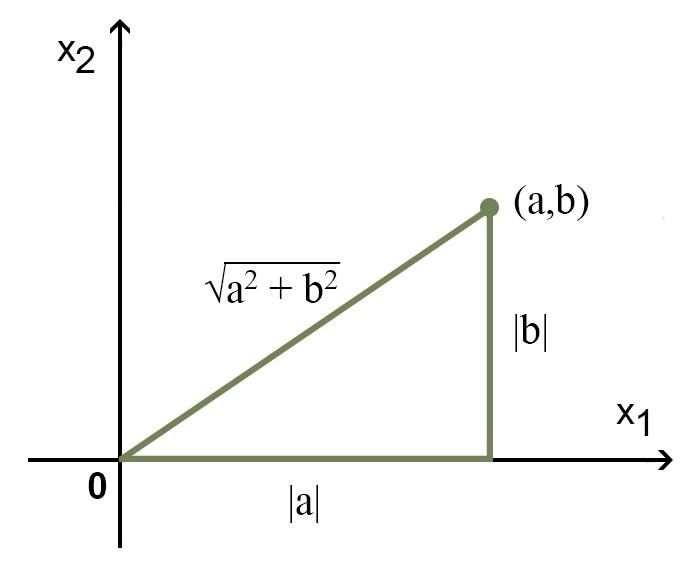
\includegraphics[width=0.50\textwidth]{Pictures/PITAGORAS.jpg}
    \caption{La norma da la longitud del vector.}
    \label{PITAGORAS}
\end{figure}

\bigskip

\begin{example}
    

El vector unitario $\vec{u} \in \mathbb{R}^4$ que tiene la misma dirección que el vector $\vec{x}$ del Ejemplo \ref{EX1chap6} es



\begin{equation}
\vec{u}=\frac{\vec{x}}{\left\| \vec{x} \right\|}=(\frac{1}{3}, -\frac{2}{3}, \frac{2}{3},0)
 \label{20}
\end{equation}
\end{example}  

\bigskip



%Ver para $\mathbb{R}^{2}$ primero Lay pag 381 y hacer gráfico

\textbf{Ángulo entre dos vectores.}\index{Angulo entre dos vectores.}


\bigskip

En $\mathbb{R}^{2}$ el producto escalar verifica la expresión que sigue:
\begin{equation}
 (\vec{x},\vec{y})   = \left\|\vec{x}\right\|\left\|\vec{y}\right\|cos \theta
 \label{30}
\end{equation}


La verificación para $\mathbb{R}^{3}$ es similar. Cuando $n > 3$, puede usarse la Ec.(\ref{30})  para
definir el ángulo entre dos vectores de $\mathbb{R}^{n}$, o en espacios vectoriales cualesquiera. 


\bigskip

Dados dos vectores $\vec{x}$ e $\vec{y}$ de un espacio euclídeo, definimos el \textit{coseno} del ángulo  entre ellos como 

\begin{equation}
cos (\theta)=\frac {(\vec{x},\vec{y})} {\left\|\vec{x}\right\|\left\|\vec{y}\right\|} 
  \label{444}
  \end{equation}


\bigskip

Para que tenga sentido la definición anterior, es necesario demostrar que el valor absoluto del cociente
\[\frac {(\vec{x},\vec{y})} {\left\|\vec{x}\right\|\left\|\vec{y}\right\|}\] 

\bigskip
\noindent
sea menor que o igual que $1$.

\bigskip
\begin{remark}
En Estadística, el valor de $cos (\theta)$ definido mediante la Ec.(\ref{444}) para los vectores $\vec{x}$ e $\vec{y}$ es llamado  \textit{coeficiente de correlación entre los vectores $\vec{x}$ e $\vec{y}$}, y mide de alguna forma la similitud entre ambos.
%\hfill$\blacktriangle$
\end{remark}

\bigskip

\index{Cauchy, Augustin Louis}
\begin{parchment}[ Augustin Louis Cauchy (1789-1857)]{Fue un matemático francés, miembro de la Academia de Ciencias de Francia y profesor en la Escuela politécnica.
Cauchy ha sido uno de los matemáticos más prolíficos de todos los tiempos, solo superado por Leonhard Euler, Paul Erdős y Arthur Cayley con cerca de 800 publicaciones y siete trabajos; su investigación cubre el conjunto de áreas matemáticas de la época. Fue pionero en análisis donde se le debe la introducción de las funciones holomorfas, los criterios de convergencia de series y las series de potencias. Sus trabajos sobre permutaciones fueron precursores de la teoría de grupos, contribuyendo de manera medular a su desarrollo. En óptica se le atribuyen trabajos sobre la propagación de ondas electromagnéticas. \cite{Cauchy}}
\end{parchment}
%{ Nació en París y murió en una villa cercana a esa misma ciudad. Fue autor de trabajos importantes sobre ecuaciones %diferenciales, series infinitas, determinantes, probabilidad, grupos de permutación y de física matemática. En 1814 %publicó una memoria que se convirtió en el fundamento de la teoría de las funciones complejas. Su trabajo se conoce %por su rigor. Publicó 789 artículos y ocupó puestos en la Facultad de Ciencias, en el Colegio de Francia y en la %Escuela Politécnica, todos en París. Existen muchos términos y teoremas que llevan su apellido. Fue un realista fiel y %vivió en Suiza, Turín y Praga. Regresó a París en 1838 y recuperó su puesto en la Academia de Ciencias. En 1848 %recuperó su lugar en la Sorbona, que mantuvo hasta su muerte.}



\bigskip

\begin{theorem}\textbf{Desigualdad de Cauchy-Schwartz:}\index{Desigualdad de Cauchy-Schwartz}
\label{PROPOSICIÓN 6.39:}



En todo espacio vectorial con producto interno, 

$$\left|{(\vec{x},\vec{y})}\right|\leq {\left\|\vec{x}\right\|\left\|\vec{y}\right\|}$$
\noindent
para todo  $\vec{x}$,$~\vec{y}$  $\in \mathbb{E}$.

\bigskip

\begin{proof}

Si $\vec{y}=\vec{0}$ vale, pues $\left|{(\vec{x},\vec{0})}\right|=0 \leq \left\|\vec{x}\right
\|0=0$.

\bigskip

Si $\vec{y}\neq \vec{0}$,

\bigskip

\[0 \leq (\vec{x}-\frac {(\vec{x},\vec{y})\vec{y}} {\left\|\vec{y}\right\|^2},\vec{x}-\frac {(\vec{x},\vec{y})\vec{y}} {\left\|\vec{y}\right\|^2})
\]
\bigskip

\[
0 \leq (\vec{x},\vec{x}-\frac {(\vec{x},\vec{y})\vec{y}} {\left\|\vec{y}\right\|^2})-\frac {(\vec{x},\vec{y})} {\left\|\vec{y}\right\|^2} (\vec{y},\vec{x}-\frac {(\vec{x},\vec{y})\vec{y}} {\left\|\vec{y}\right\|^2})
\]

\bigskip

\[0 \leq (\vec{x},\vec{x})- \overline{(\vec{x},\vec{y}}+\frac {(\vec{x},\vec{y})} {\left\|\vec{y}\right\|^2}  - \frac {(\vec{x},\vec{y})} {\left\|\vec{y}\right\|^2}(\vec{y},\vec{x}) + \frac {(\vec{x},\vec{y})} {\left\|\vec{y}\right\|^2}\frac {\overline{(\vec{x},\vec{y})}} {\left\|\vec{y}\right\|^2}(\vec{y},\vec{y})
\]

\bigskip


\[0 \leq (\vec{x},\vec{x})- \overline{(\vec{x},\vec{y})}\frac {(\vec{x},\vec{y})} {\left\|\vec{y}\right\|^2}  - \frac {(\vec{x},\vec{y})} {\left\|\vec{y}\right\|^2}(\vec{y},\vec{x}) + \frac {(\vec{x},\vec{y})} {\left\|\vec{y}\right\|^2}\frac {{(\vec{y},\vec{x})}} {\left\|\vec{y}\right\|^2}(\vec{y},\vec{y})
\]

\bigskip


Como $\left\|\vec{y}\right\|^2=(\vec{y},\vec{y})$, se cancelan los dos últimos términos. Entonces,

\bigskip

\[0 \leq \left\|\vec{x}\right\|^2 - \frac {\left|{(\vec{x},\vec{y})}\right|^2} {\left\|\vec{y}\right\|^2}
\]
\noindent
que equivale a 

\[0 \leq  \frac {\left\|\vec{x}\right\|^2 \left\|\vec{y}\right\|^2 -\left|{(\vec{x},\vec{y})}\right|^2} {\left\|\vec{y}\right\|^2}
\]
\bigskip

En el numerador se tiene la desigualdad que se quería demostrar.

\end{proof}
\end{theorem}







\begin{remark}
Se acredita a Cauchy la desigualdad para vectores y a Schwarz para los productos escalares con integrales. Sin embargo, fue Bunyakovsky quien demostró y publicó la desigualdad de Schwarz en una monografía, 25 años antes que Schwarz.
%\hfill$\blacktriangle$   
\end{remark}

\bigskip







\section{Distancia entre vectores.}

\bigskip

\begin{definition}\index{Distancia entre vectores}
%\textbf{Distancia entre vectores}



Sea $V$ un espacio vectorial sobre $\mathbb{R}$ o $\mathbb{C}$ con producto interno. Se define la distancia $d$, $d :  V \times V\rightarrow \mathbb{R}$  como:

$$d(\vec{x},\vec{y})=\left\|\vec{x}-\vec{y}\right\|.$$
\end{definition}

\bigskip

Usando las propiedades de la norma, se puede verificar que $d$ satisface:

\bigskip

\begin{enumerate}

\item   $d(\vec{x},\vec{y}) \geq 0 $  para todo $\vec{x}$,$~\vec{y}$ $\in E$

\bigskip

\item   $d(\vec{x},\vec{y})= 0 $  sí y sólo sí  $\vec{x}=\vec{y}$ 

\bigskip

\item   $d(\vec{x},\vec{y})= d(\vec{y},\vec{x})$  para todo $\vec{x}$,$~\vec{y}$ $\in E$

\bigskip

 \item  $d(\vec{x},\vec{z})\leq d(\vec{x},\vec{y})+ d(\vec{y},\vec{z})   $  para todo $\vec{x}$, $~\vec{y}$, $~\vec{z}$ $\in E$.

\bigskip

\bigskip

\bigskip

\end{enumerate}

\index{Schwarz, Karl  Herman  }
\begin{parchment}[Karl Herman Amandus Schwarz (1843-1921)] {Fue un matemático alemán conocido por su trabajo en análisis complejo. Schwarz inicialmente estudio química en Berlín pero Kummer y Weierstrass lo persuadieron para que se hiciera matemático. Entre 1867 y 1869 trabajó en Halle, después en Zürich. Desde 1875 trabajó en el universidad de Gotinga, tratando los temas de teoría de funciones, geometría diferencial y cálculo de variaciones. Su memoria en ocasión del 70 aniversario de Weierstrass contiene, entre otros temas importantes, la desigualdad para integrales que hoy se conoce como desigualdad de Schwarz. \cite{schwarz} }
\end{parchment}




\bigskip




\index{Bunyakovsky, Viktor Yakovlevich}
\begin{parchment}[Viktor Yakovlevich Bunyakovsky (1804-1889)]{ Nació en Ucrania. Estudió matemáticas en la Sorbona, en la que se doctoró en 1825 bajo la tutoría de Augustin Cauchy.1​
En 1826 volvió a San Petersburgo donde ejerció como profesor de la Escuela de Cadetes de la Academia Naval y del Instituto de Comunicaciones. De 1846 a 1880 fue profesor en la Universidad de San Petersburgo. 

Entre otros campos de las matemáticas, Buniakovski trabajó sobre todo en teoría de números, análisis matemático y en teoría de la probabilidad. Son relevantes las aportaciones que llevan su nombre como la conjetura de Buniakovski (nunca demostrada) y la desigualdad de Cauchy-Buniakovski-Schwarz. Sus aportaciones más originales son en teoría de la probabilidad, acerca de la cual publicó numerosos artículos sobre el estudio de problemas estadísticos de la población de Rusia. \cite{buny}   } 
\end{parchment}


\bigskip

\bigskip






\begin{figure}
    \centering
    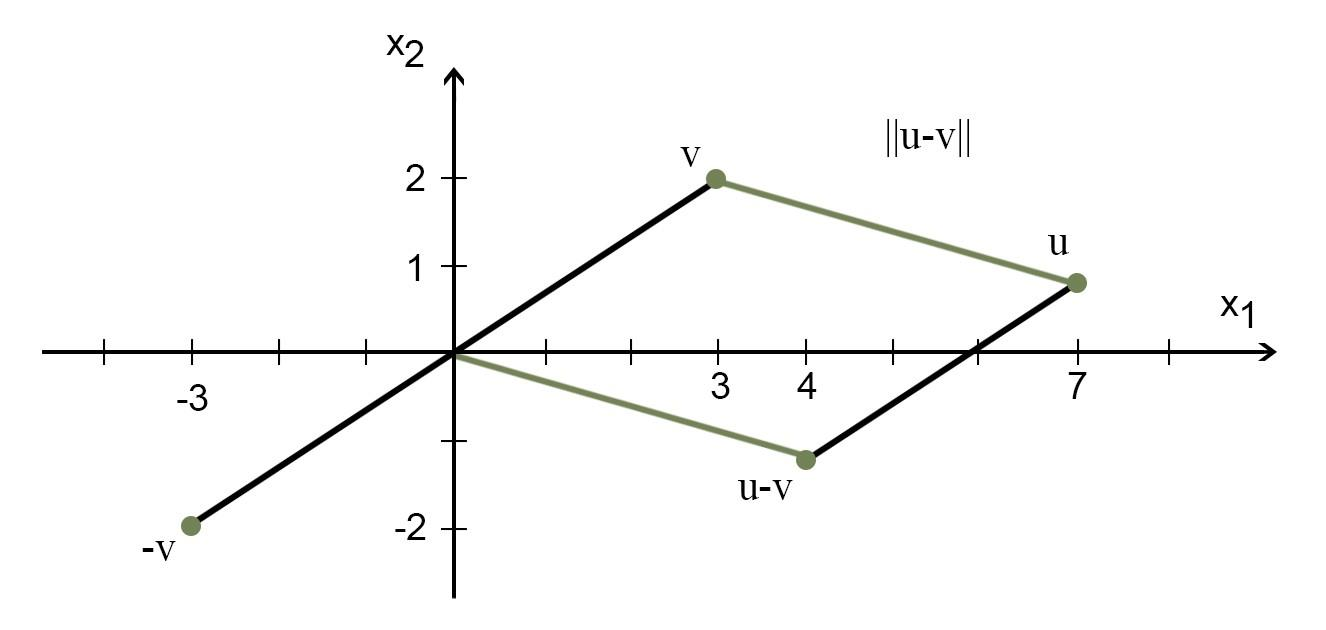
\includegraphics[width=0.80\textwidth]{Pictures/DISTANCIA.jpg}
    \caption{Distancia entre los vectores $\vec{u}$ y $\vec{v}$. }
    \label{DISTANCIA}
\end{figure}

\bigskip

\begin{example}
    

En la Figura \ref{DISTANCIA} se muestran los vectores $\vec{u}$, $\vec{v}$ y $\vec{u}- \vec{v}$,

$$ \vec{u}- \vec{v}= \left(\begin{array}{c}  7  \\ 1
\end{array}
 \right)-   \left(\begin{array}{c}  3  \\ 2 
\end{array}
 \right) =   \left(\begin{array}{c}  4  \\ -1
\end{array}
 \right)$$ 

$$\left\|\vec{u}-\vec{v}\right\|= \sqrt{ 4^4+ (-1)^2}=\sqrt{17}.$$

Puede observarse que la distancia de $\vec{v}$ a $\vec{u}$ es la misma que la de $\vec{u}- \vec{v}$ a $\vec{0}$, y también que si se suma el vector $\vec{u}- \vec{v}$ a $\vec{v}$ se obtiene el vector $\vec{u}$.
\end{example} 

\begin{remark}
\begin{itemize}
    \item 

     Dados dos vectores   $\vec{x}$ e $\vec{y}$, se dice que $d(\vec{x},\vec{y})$ es la \textit{distancia} entre $\vec{x}$ e $\vec{y}$.
     \item 

     Una distancia es una función  que verifica las $4$ propiedades anteriores. Puede no provenir de ninguna norma.
\end{itemize}
 %\hfill$\blacktriangle$   
\end{remark}






\bigskip

Con la definición que sigue se  generaliza  la noción de perpendicularidad entre vectores de un espacio vectorial. 

\bigskip
\begin{definition}

Sea $V$ un espacio vectorial sobre $\mathbb{R}$ o $\mathbb{C}$ con producto interno. Dos vectores $\vec{x}$, $\vec{y}$ se dicen \textit{ortogonales} (o perpendiculares), si
\begin{equation}
(\vec{x},\vec{y})=0
\label{40}
\end{equation}

\end{definition}

\bigskip

\begin{remark}
Por las propiedades vistas en las  observaciones \textcolor{blue}{{\fontfamily{qcr}\selectfont{i}}} en la Sección \ref{ObsPI}, el vector nulo,  es ortogonal a todo vector de $V$.
%\hfill$\blacktriangle$   
\end{remark}




\begin{corollary}
    
\textbf{Teorema de Pitágoras} 
\label{Pitagoras}


Dos vectores $\vec{x}$ e $\vec{y}$  son ortogonales, sii 

$$\left\|\vec{x}+\vec{y}\right\|^{2}=\left\|\vec{x}\right\|^{2}+\left\|\vec{y}\right\|^{2}$$

\end{corollary}

\bigskip

La demostración se deja al lector.


\bigskip


\begin{definition} 

Sea $V$ un espacio vectorial sobre $\mathbb{R}$ o $\mathbb{C}$ de dimensión finita con producto interno. Se dice que $\left\{\vec{v}_1,\vec{v}_2,\cdots, \vec{v}_r\right\}\subset V$ es un conjunto ortogonal si $(\vec{v}_i,\vec{v}_j)=0$ para todo $i\neq j$. \end{definition}

\bigskip

\begin{example}
 \label{eju1u2u3}   

El conjunto  $S=\{\vec{u_1}, \vec{u_2}, \vec{u_3}\}$, 
donde $\vec{u_1}=(3,1,1)^T$, $\vec{u_2}=(-1,2,1)^T$ y $\vec{u_3}=(-1/2,-2,7/2)^T$,
es un conjunto ortogonal, ya que al considerar los tres pares posibles de vectores, 

\bigskip

$\{\vec{u_1}, \vec{u_2}\}$, $\{\vec{u_1},\vec{u_3}\}$, y $\{\vec{u_2}, \vec{u_3}\}$, se tiene 

 \bigskip 

$\vec{u}_1 \cdot \vec{u}_2= 3(−1) + 1(2) + 1(1)= 0$

\bigskip

$\vec{u}_1 \cdot \vec{u}_3= 3(−1/2) + 1(-2) + 1(7/2)= 0$

\bigskip

$\vec{u}_2 \cdot \vec{u}_3= -1(−1/2) + 2(-2) + 1(7/2)= 0$

\bigskip



Cada par de vectores distintos es ortogonal, así que $S=\{\vec{u_1}, \vec{u_2}, \vec{u_3}\}$, es un conjunto ortogonal como se muestra  en  la Figura \ref{Conj.Ortog}. 
\end{example}



\begin{figure}
    \centering
    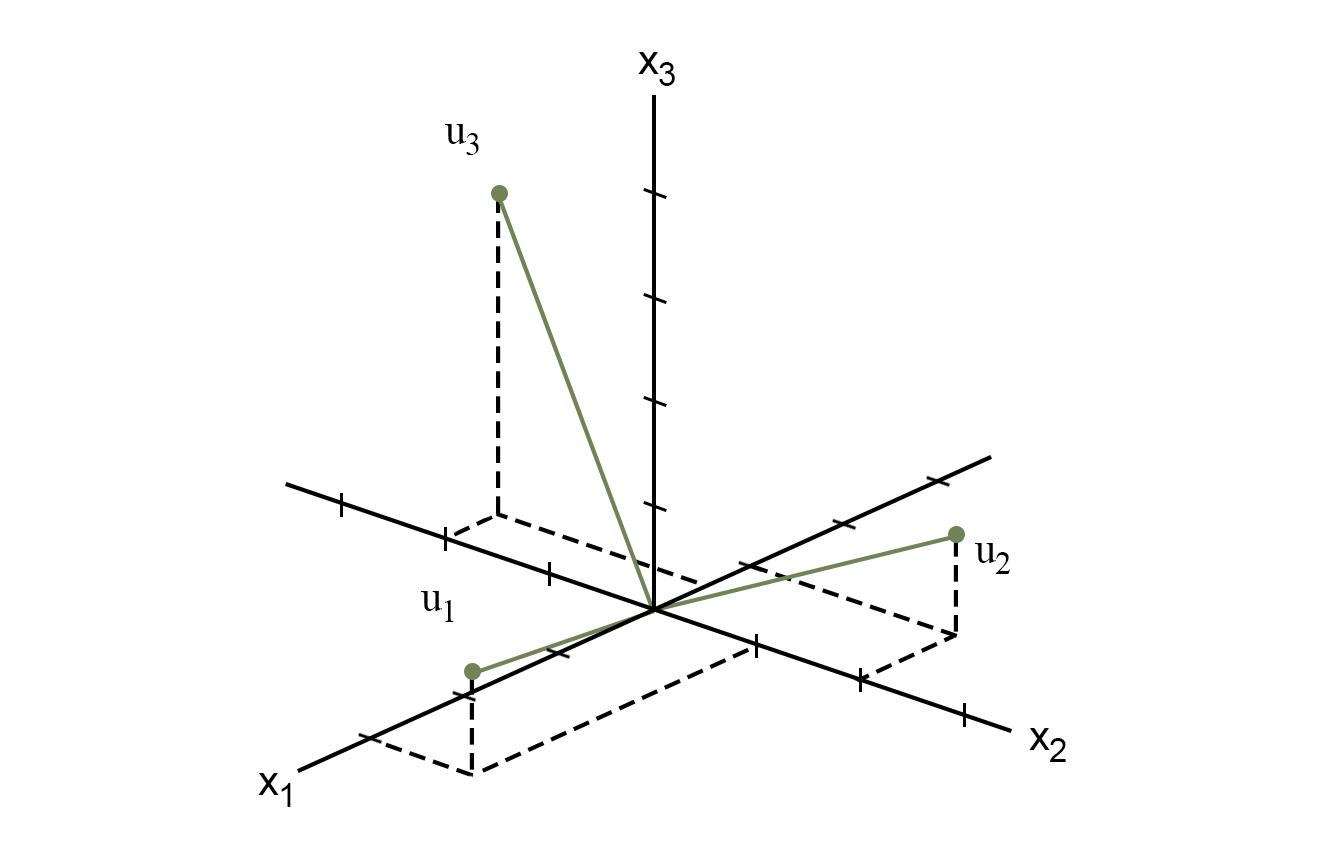
\includegraphics[width=0.80\textwidth]{Pictures/fig.28.jpg}
    \caption{$\{\vec{u_1}, \vec{u_2}, \vec{u_3}\}$ es un conjunto ortogonal de $\mathbb{R}^3$.}
    \label{Conj.Ortog}
\end{figure}

\bigskip

\begin{remark}
Un conjunto de $r$ vectores se dice \textit{ortonormal} si es ortogonal y $\left\|\vec{u}_i\right\|=1$  para cada $1\leq i\leq r$.
%\hfill$\blacktriangle$  
\end{remark}

\bigskip

\begin{theorem}

Sea $V$ un espacio vectorial sobre $\mathbb{R}$ o $\mathbb{C}$ de dimensión finita con producto interno y sea $\left\{\vec{v}_1,\vec{v}_2,\cdots, \vec{v}_r\right\}\subset V$  un conjunto ortogo-\ nal de $V$ con $\vec{v}_i\neq \vec{0}$  para  $1\leq i\leq r$. Entonces  $\left\{\vec{v}_1,\vec{v}_2,\cdots, \vec{v}_r\right\}$ es un conjunto de vectores  linealmente independiente.

\begin{proof}

Supongamos que $\sum_{i=1}^r  \alpha_i \vec{v}_i = \vec{0}$. Entonces, para cada $j$, $ 1 \leq j \leq r$,


$$ 0=(\vec{0}, \vec{v}_j)= ( \sum_{i=1}^r  \alpha_i \vec{v}_i,\vec{v}_j) = \sum_{i=1}^r  \alpha_i (\vec{v}_i,\vec{v}_j )= \alpha_j \left\|\vec{v}_j\right\|^{2}, $$

\noindent
y como $\vec{v}_j \neq \vec{0}$,  $ \alpha_j=0$ para  $ 1 \leq j \leq r$ y entonces, $\left\{\vec{v}_1,\vec{v}_2,\cdots, \vec{v}_r\right\}$ es un conjunto de vectores linealmente independiente.

 
\end{proof}

\end{theorem}

\bigskip

En el teorema siguiente se muestra por qué una base ortogonal es mucho mejor que otras bases: las coordenadas de un vector en esa base  pueden calcularse muy  fácilmente.

\bigskip


\begin{theorem}

Sea $V$ un espacio vectorial sobre $\mathbb{R}$ o $\mathbb{C}$ de dimensión finita con producto interno y sea $\left\{\vec{v}_1,\vec{v}_2,\cdots, \vec{v}_r\right\}\subset V$ es un conjunto ortogonal de $V$ con $\vec{v}_i\neq \vec{0}$  para  $1\leq i\leq r$. Sea $\vec{v} \in \left\langle \vec{v}_1,\vec{v}_2,\cdots, \vec{v}_r\right\rangle$. Entonces 


\begin{equation}
  \vec{v} =\sum^{r}_{j=1}   \frac {(\vec{v}, \vec{v}_j)} {\left\|\vec{v}_j\right\|^{2}} \vec{v}_j
  \label{50}
\end{equation}


\begin{proof}
 Si  $ \vec{v} = \sum_{i=1}^r  \alpha_i \vec{v}_i$, para cada $j$, $ 1 \leq j \leq r$, se tiene que 

 $$ (\vec{v}, \vec{v}_j)= ( \sum_{i=1}^r  \alpha_i \vec{v}_i,\vec{v}_j) = \sum_{i=1}^r  \alpha_i (\vec{v}_i,\vec{v}_j )= \alpha_j (\vec{v}_i,\vec{v}_j ) =\alpha_j \left\|\vec{v}_j\right\|^{2}, $$

\noindent 
 y como $\vec{v}_j\neq \vec{0}$, se tiene entonces que \[\alpha_j = \frac{(\vec{v}, \vec{v}_j)}{\left\|\vec{v}_j\right\|^{2}}\]
\end{proof}

\end{theorem}

\bigskip


\begin{example}
\label{EJ48}
El conjunto $\{\vec{u_1}, \vec{u_2}, \vec{u_3}\}$  del Ejemplo \ref{eju1u2u3}   es una base ortogonal para
$\mathbb{R}^3$. Si se  desea expresar el vector $\vec{y}=(6,1,-8)^T$ como una combinación lineal de los vectores en $S$,
de acuerdo a la  Ec.(\ref{50}) se tiene que, 

\begin{equation*}
  \vec{y} =\sum^{3}_{j=1}   \frac {(\vec{y}, \vec{u}_j)} {\left\|\vec{u}_j\right\|^{2}} \vec{u}_j
  \label{60}
\end{equation*}

\bigskip

Para hallar las coordenadas de $\vec{y}$ en la base ortogonal,   se  calculan los productos escalares

\bigskip

$\vec{y}. \vec{u_1}= 11$, $\vec{y}. \vec{u_2}= -12$, $\vec{y}. \vec{u_3}= -33$

\bigskip
y 
$\vec{u_1}. \vec{u_1}= 11$, $\vec{u_2}. \vec{u_2}= 6$, $\vec{u_3}. \vec{u_3}= 33/2$



 \bigskip

\begin{equation*}
  \frac {(\vec{y}, \vec{u}_1)} {\left\|\vec{u}_1\right\|^{2}} \vec{u}_1=\frac{11}{11}(3,1,1) =(3,1,1)
  \label{70}
\end{equation*}

\begin{equation*}
  \frac {(\vec{y}, \vec{u}_2)} {\left\|\vec{u}_2\right\|^{2}} \vec{u}_2=\frac{-12}{6}(-1,2,1)=2(-1,2,1)
  \label{70}
\end{equation*}

\begin{equation*}
   \frac {(\vec{y}, \vec{u}_3)} {\left\|\vec{u}_3\right\|^{2}} \vec{u}_3=\frac{-33}{33/2}(-1/2,-2,7/2)=2(-1/2,-2,7/2)
  \label{80}
\end{equation*}

Y se obtiene, 
\[
\vec{y}= 1 \vec{u}_1 -2 \vec{u}_2 -2 \vec{u}_3 
\]
\noindent
que puede verificarse fácilmente,

$\vec{y}=(6,1,-8)=(3,1,1) -2(-1,2,1) -2 (-1/2,-2,7/2)$.
\end{example}

\bigskip

\begin{remark}
 \begin{itemize}
     \item

     Como se vio en el Ejemplo  \ref{EJ48}, es muy  fácil  calcular las coordenadas de un vector $\vec{y}$ en una base ortogonal. En otro caso,  se debe que resolver un sistema de ecuaciones lineales para hallarlas.
\item
Si el conjunto además, es ortonormal, se tiene

$$ \vec{v} =\sum^{r}_{j=1}   (\vec{v}, \vec{v}_j)  \vec{v}_j $$
 \end{itemize}
 %\hfill$\blacktriangle$
\end{remark}

\bigskip

\bigskip

La proposición que sigue asegura que en todo espacio vectorial de dimensión finita con producto interno tiene  bases ortonormales. Más aún, en la demostración se da un procedimiento recursivo conocido como Gram-Schmidt que permite obtener una base ortonormal del espacio vectorial a partir de una base cualquiera del mismo.


\bigskip

\begin{theorem}
\textbf{ Método de ortonormalización de Gram-Schmidt} \index{Método  de Gram-Schmidt} 

\bigskip

Sea $V$ un espacio vectorial sobre $\mathbb{R}$ o $\mathbb{C}$ de dimensión finita con producto interno y sea $\left\{\vec{v}_1,\vec{v}_2,\cdots, \vec{v}_n\right\}$ una base de $V$. Existe una base ortonormal $B= \left\{\vec{w}_1,\vec{w}_2,\cdots, \vec{w}_n\right\}$ de $V$ tal que 

$$\left\langle \vec{v}_1,\vec{v}_2,\cdots, \vec{v}_k \right\rangle  = \left\langle \vec{w}_1,\vec{w}_2,\cdots, \vec{w}_k \right\rangle $$
para todo $1\leq k \leq n$

%La base ortonormal se obtiene normalizando los vectores de $B$ (dividiendo cada vector de $B$ por su %longitud).


\begin{proof}

Se construyen los vectores  $\left\{\vec{z}_1,\vec{z}_2,\cdots, \vec{z}_n\right\}$ de una base ortogonal, recursivamente



\begin{enumerate}

\item Se toma $\vec{z}_1=\vec{v}_1$  

\bigskip

\item  Se busca $\vec{z}_2 \in V$ tal que $(\vec{z}_2, \vec{z}_1)=0$ y tal que 
$\left\langle \vec{z}_1,\vec{z}_2\right\rangle=\left\langle \vec{v}_1,\vec{v}_2\right\rangle$




\end{enumerate}

\bigskip


La segunda condición vale sí y sólo sí $~\vec{z}_2=a\vec{v}_1+b\vec{v}_2$ con $b\neq 0$. Es  posible considerar $b=1$ y buscar $a$ para que se cumpla la primera condición:

\bigskip



$0=(\vec{z}_2, \vec{z}_1)=(a\vec{v}_1+b\vec{v}_2, \vec{z}_1)= a(\vec{v}_1,\vec{v}_1)+(\vec{v}_2,\vec{v}_1)$,

\noindent 
lo que implica 



$$ a=  \frac {-(\vec{v}_2, \vec{v}_1)} {\left\|\vec{v}_1\right\|^{2}}. $$



Luego, el vector, 

$$ \vec{z}_2= \vec{v}_2 - \frac {(\vec{v}_2, \vec{v}_1)} {\left\|\vec{v}_1\right\|^{2}} \vec{v}_1= \vec{v}_2 - \frac {(\vec{v}_2, \vec{v}_1)} {\left\|\vec{v}_1\right\|^{2}} \vec{z}_1$$
\noindent
satisface las condiciones.

\bigskip


Supongamos construídos $\vec{z}_1, \vec{z}_2,   \cdots, \vec{z}_r \in V$  tales que 

\bigskip

\begin{enumerate}

\bigskip

\item $(\vec z_i,\vec z_j)=0$  cuando $i\neq j$

\bigskip

\item   $\left\langle \vec z_1,\vec z_2, \cdots, \vec z_r \right\rangle=\left\langle \vec v_1,\vec v_2, \cdots, \vec v_r\right\rangle$   con $1\leq k \leq r$


\end{enumerate}
\bigskip

\noindent
consideramos el vector

$$ \vec{z}_{r+1}= \vec{v}_{r+1} -\sum^{r}_{i=1} \frac {(\vec{v}_{r+1}, \vec{z}_i)} {\left\|\vec{z}_i\right\|^{2}} \vec{z}_i$$


\bigskip

Se tiene que 


\bigskip

\begin{itemize}

\item 
$\left\langle \vec{z}_1,\vec{z}_2, \cdots, \vec{z}_r, \vec{z}_{r+1} \right\rangle=\left\langle \vec{v}_1,\vec{v}_2, \cdots, \vec{v}_r,\vec{v}_{r+1}\right\rangle$   con $1\leq k \leq r$

\bigskip

\item  para cada $j\leq r$,  reemplazando $\vec{z}_{r+1}$ y teniendo en cuenta $1.$, 

$$(\vec{z}_{r+1}, \vec{z}_j)=( \vec{v}_{r+1} -\sum^{r}_{i=1} \frac {(\vec{v}_{r+1}, \vec{z}_i)} {\left\|\vec{z}_i\right\|^{2}} \vec{z}_i, \vec{z}_j)$$


$$(\vec{z}_{r+1}, \vec{z}_j)=( \vec{v}_{r+1},, \vec{z}_j) - \frac {(\vec{v}_{r+1}, \vec{z}_j)} {\left\|\vec{z}_j\right\|^{2}}( \vec{z}_j, \vec{z}_j)=0$$


\end{itemize}

\bigskip

Luego $\vec{z}_{r+1}$ satisface las condiciones requeridas.

\bigskip

De esta manera, al concluir el $n$-ésimo paso, se obtiene una base ortogonal $\left\{\vec{z}_1,\vec{z}_2,\cdots, \vec{z}_n\right\}$ de $V$ que además satisface

$$\left\langle \vec{v}_1,\vec{v}_2,\cdots, \vec{v}_k \right\rangle  = \left\langle \vec{z}_1,\vec{z}_2,\cdots, \vec{z}_k \right\rangle $$
para todo $1\leq k \leq n$.

\bigskip

Finalmente, para cada $1\leq i \leq n$ consideramos el vector   $\vec{w}_i=\frac {\vec{z}_i} {\left\|\vec{z}_i \right\|}$. Luego, el conjunto $B= \left\{\vec{w}_1,\vec{w}_2,\cdots, \vec{w}_n\right\}$ resulta una base de $V$ que cumple lo pedido.

\end{proof}
\end{theorem}



\bigskip


\bigskip


\textcolor{blue}{\textbf{Corolario}}
Sea $V$ un espacio vectorial sobre $\mathbb{R}$ o $\mathbb{C}$ de dimensión finita con producto interno y sea $S$ un subespacio   de $V$, $S\neq \{\vec{0}\}$. Entonces existe una base ortonormal de $V$ que contiene una base ortonormal de $S$.
Se demuestra tomando una base de $S$, completando a una base de $V$ y aplicando a esta base el procedimiento de Gram-Schmidt.
{\hfill{\tiny\ensuremath{\blacksquare}}

\bigskip

\bigskip

%\end{document}



\begin{example} \textbf{Aplicación del  Método de Gram-Schmidt}

\bigskip

Dada la base $B= \left\{(1,0,i),(1,1,2+i),(0,0,1)\right\}$ de $\mathbb{C}^{3}$ se desea hallar una base ortonormal con G-S.

\bigskip

$\vec{v}_1= (1,0,i)  $, $\vec{v}_2= (1,1,2+i)$    y $\vec{v}_3=(0,0,1)$ 

\bigskip






$\vec{z}_{1}= \vec{v}_{1}$



\[
 \vec{z}_{2}= \vec{v}_{2} -\frac {(\vec{v}_2, \vec{z}_1)} {\left\|\vec{z}_1\right\|^{2}} \vec{z}_1 
\]



\[\vec{z}_{2}= (1,1,2+i) -\frac {((1,1,2+i), (1,0,i))} {\left\|(1,0,i)\right\|^{2}} (1,0,i)
\]


\[\vec{z}_{2}= (1,1,2+i) -(1-i) (1,0,i)=(i,1,1)
\]


y luego, 




\[ \vec{z}_{3}= \vec{v}_{3} - \frac {(\vec{v}_{3}, \vec{z}_1)} {\left\|\vec{z}_1\right\|^{2}} \vec{z}_1 - \frac {(\vec{v}_{3}, \vec{z}_2)} {\left\|\vec{z}_2\right\|^{2}} \vec{z}_2 
\]
\bigskip


$ \vec{z}_{3}=(i/6,-1/3,1/6)$

\bigskip

$\left\{\vec{z}_1,\vec{z}_2, \vec{z}_3\right\}$ resulta una base de ortogonal de $\mathbb{C}^{3}$ 

\bigskip

Diviendo por su norma queda una base ortonormal $\left\{\vec{w}_1,\vec{w}_2, \vec{w}_3\right\}$

\bigskip

donde $\vec{w}_1=(1/\sqrt{2},0,i/\sqrt{2})$

\bigskip

$\vec{w}_2=(i/\sqrt{3},1/\sqrt{3} , 1/\sqrt{3})$

\bigskip

$\vec{w}_3=(\sqrt{6}i/6,-\sqrt{6}/3 , \sqrt{6}/6)$
  
\end{example}

\bigskip

\bigskip
%\end{document}
La existencia de bases ortogonales para subespacios de dimensión finita de un espacio
con producto interior puede establecerse por medio del proceso Gram-Schmidt, de igual
forma que en $\mathbb{R}^n$. Al aplicar este proceso, es posible plantear ciertas bases ortogonales
que surgen con frecuencia en las aplicaciones y  construir la proyección ortogonal de un vector sobre un subespacio $S$. La proyección no depende de la selección de la
base ortogonal y tiene muy buenas propiedades que se describirán más adelante.
%descritas en el teorema de la descomposición
%ortogonal y en el teorema de la mejor aproximación (ver).
En el teorema que sigue se ve cómo es posible escribir la matriz de una transformación lineal usando producto interno para escribir las coordenadas de la imagen de cada vector de la base ortogonal.

\bigskip

\begin{corollary}
    

Si $T$ es una transformación lineal sobre $V$, $V$ es un espacio vectorial con producto interno y de 
dimensión finita, entonces

$$ (T)_B=((T(\vec{u_j}),\vec{u_i})_{ij}$$
siendo $B=\{\vec{u_1}, \vec{u_2},\cdots  \vec{u_n}\}$ cualquier base ortonormal de $V$.

\begin{proof}
$T(\vec{u}_1)=k_1\vec{u}_1+k_2\vec{u}_2+ \cdots +k_n\vec{u}_n.$

\bigskip

En la primer columna de la matriz deben ir las coordenadas   de $T(\vec{u}_1)$, o sea  $k_1$,  $\cdots  k_n$.

\bigskip
\noindent
y resulta que, las coordenadas son

\bigskip

$(T(\vec{u}_1),\vec{u}_i )= T(k_1\vec{u}_1+k_2\vec{u}_2\cdots+k_n\vec{u}_n,\vec{u}_i)$

\bigskip

$=k_1 (\vec{u}_1,\vec{u}_1) +  k_2 (\vec{u}_1,\vec{u}_2) + \cdots  k_n (\vec{u}_1,\vec{u}_n) = k_i$

\end{proof}
\end{corollary}


\bigskip

\subsection{Complemento Ortogonal}\index{Complemento ortogonal}

\bigskip


\begin{definition}\index{Complemento ortogonal}
    Sea $V$ un espacio vectorial sobre $\mathbb{R}$ o $\mathbb{C}$  con producto interno y sea $S$ un subespacio de $V$. Se define el complemento ortogonal de $S$ como 


\bigskip

$S^{\perp} = \left\{\vec{v}\in V \quad (\vec{v}, \vec{s})=0 \quad \forall \vec{s} ~\in S \right\}$
\end{definition}
\bigskip

\begin{remark}
$S^{\perp}$ es un subespacio de $V$.
\end{remark}  





\begin{example}
Para el subespacio de  $\mathbb{R}^{2}$ generado por el vector $(1,1)$, su complemento ortogonal es  $\left\langle (1,1)\right\rangle^{\perp}=\left\{(x,y) \in \mathbb{R}^{2}, ((x,y),(1,1))=0 \right\}= \left\{(x,y) \in \mathbb{R}^{2}, \quad x+y=0 \right\}=\left\langle (1,-1)\right\rangle$.
\end{example}


\bigskip

\begin{example}
Sea $W$ un plano que pasa por el origen en $\mathbb{R}^3$, y sea $L$ la recta que pasa
por el origen y es perpendicular a $W$. Si $\Vec{u}_1$ y $\Vec{u}_2$ son diferentes de $\Vec{0}$, $\Vec{u}_1$ está sobre $L$, y $\Vec{u}_2$ está en $W$, $\Vec{u}_1 \cdot \Vec{u}_2= 0$, como se muestra en la  Figura \ref{321PROYORTOG}. Así que cada vector sobre $L$ es ortogonal a cada vector $\Vec{w}$ en $W$. De hecho, $L$ consiste en todos los vectores que son ortogonales a los $\Vec{w}$ en
$W$, y $W$ consiste en todos los vectores ortogonales a los vectores  en $L$. Es decir,
$L = W^{\perp}$ y $W = L^{\perp}$. ❚
\end{example} 




\begin{figure}
    \centering
    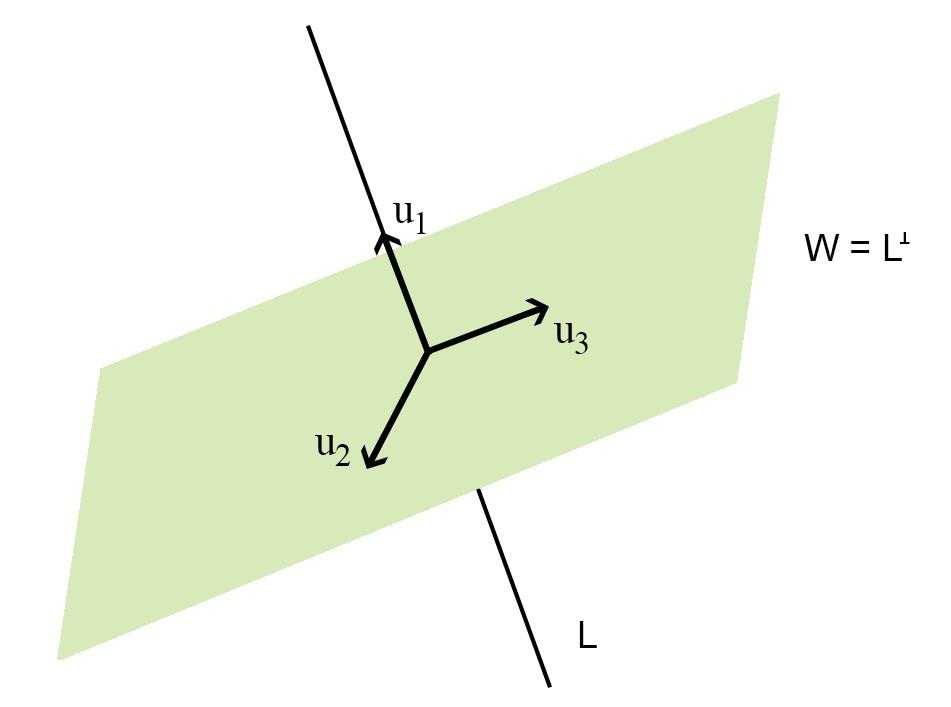
\includegraphics[width=0.80\textwidth]{Pictures/fig.321.jpg}
    \caption{Complemento ortogonal.}
    \label{321PROYORTOG}
\end{figure} 


\bigskip

\begin{example}
%Ejemplo hojita 36
En $\mathbb{C}^3$ hallar el complemento ortogonal de $ \langle( 1,i,1+i) \rangle$.
$ \langle( 1,i,1+i) \rangle^t =$
\begin{eqnarray*}
   = \left \{ (x_1,x_2,x_3) \in \mathbb{C}^3, (x_1,x_2,x_3) \cdot (\alpha , \alpha i, \alpha (1+i))=0 \quad \forall \alpha \in \mathbb{C} \right \} \\
     = \left \{ (x_1,x_2,x_3) \in \mathbb{C}^3, x_1 \overline{\alpha} + x_2 \overline{\alpha i }  + x_3  \overline{\alpha}   (\overline{1+i})=0 \quad \forall \alpha \in \mathbb{C} \right \} 
\end{eqnarray*}
De donde  $$   x_1 \overline{\alpha} - x_2 \overline{\alpha} i + x_3 \overline{\alpha} (1-i)=0$$
o 
 $$    \overline{\alpha}( x_1 - x_2 i + x_3 (1-i))=0.$$
 
 Se tiene, entonces, $x_1= x_2 i - x_3 (1-i)$ y resulta 
\begin{eqnarray*}
    \langle( 1,i,1+i) \rangle^t =  \left \{ (x_2 i - x_3 (1-i), x_2, x_3 )= x_2(i,1,0) + x_3 (i-1,0,1) \right \}
\end{eqnarray*}
\end{example}

\bigskip
\index{Espacio columna de una matriz}
\begin{corollary}
Sea $A$ una matriz de $m \times  n$. El complemento ortogonal del espacio fila de $A$, $Fil A$,  (subespacio de $\mathbb{R}^{n}$ que generan los vectores filas de $A$) es
el espacio nulo de $A$, $Nul(A)$ y el complemento ortogonal del espacio columna de $A$, $Col A$, (subespacio de $\mathbb{R}^{m}$ que generan los vectores columnas de $A$) es el
espacio nulo de la matriz $A^T$. Es decir,



\bigskip

$(Fil A)^{\perp} = Nul(A)$ y $(Col A)^{\perp} = Nul(A^T)$
\end{corollary}



\bigskip

\bigskip

\begin{example}
Dada la matriz


\begin{equation}
A= \left(\begin{array}{ccc} 1  & 0  & 2  \\ 1 & 1 & 4
\end{array}
 \right), \label{333}
\end{equation}
\end{example}

\bigskip
\noindent
se describen los espacios $(Fil A)$, $ Nul(A)$ y $(Col A):


$Nul(A)$ son los vectores de $\mathbb{R}^{3}$ soluciones del sistema homogéneo. Esos vectores son perpendiculares a las filas de la matriz $A$, y pertenecen entonces a subespacio $(Fil A)^{\perp}$.

Si ahora se resuelve el sistema homogéneo con la matriz $A^T$, da el vector nulo de $\mathbb{R}^{2}$.
El subespacio que generan las columnas de $A$, $Col A$ es todo $\mathbb{R}^{2}$, pues  hay en las columnas $2$ vectores linealmente independientes. De ahí que el subespacio ortogonal,  $(Col A)^{\perp} = Nul(A^T)= \vec{0}$.

\bigskip

\bigskip

\begin{theorem}

Sea $V$ un espacio vectorial de dimensión finita con producto interno y sea $S\subseteq V$ un subespacio. Entonces


\bigskip

\begin{enumerate}

\item $S \cap S^{\perp} =\vec{0}$

\bigskip

\item $dim(S) + dim(S^{\perp}) = dim(V)$

\end{enumerate}

\bigskip

En consecuencia, $S \oplus S^{\perp}$.

\bigskip

\begin{proof}

\bigskip
\begin{itemize}
    \item 
  Sea   $\vec{v} \in S \cap S^{\perp}$. Como $\vec{v} \in  S^{\perp}$, $(\vec{v},\vec{s})=0$, $\forall \vec{s}\in S$. En particular para $\vec{s}=\vec{v}$, entonces $(\vec{v},\vec{v})=\left\|\vec{v}\right\|^2=0$, de donde $\vec{v}=\vec{0}$.

  \bigskip
     \item 
   Sea $\left\{\vec{s}_1,\vec{s}_2,\cdots,\vec{s}_r\right\}$ una base de $S$. Existen 
   $\vec{v}_{r+1}, \cdots,\vec{v}_n$ tales que \\ $B=\left \{\vec{s}_1,\vec{s}_2,\cdots,\vec{s}_r,\vec{v}_{r+1}, \cdots,\vec{v}_n \right \}$ es una base de $V$. 
   
   Aplicando Gram-Schmidt se obtiene una base ortonormal  de $V$, 
    $B^\prime=\left\{\vec{w}_1,\vec{w}_2,\cdots,\vec{w}_r,\vec{w}_{r+1}, \cdots\vec{w}_n\right\}$ tal que  $$\left\langle \vec{w}_1,\vec{w}_2,\cdots, \vec{w}_r \right\rangle  = \left\langle \vec{s}_1,\vec{s}_2,\cdots, \vec{s}_r \right\rangle=S.$$
    Sea $j > r$. Veamos que $\vec{w}_j \in S^{\perp}$.
    Dado $\vec{s} \in S$, existen escalares $\alpha_1,\cdots,\alpha_r$, tales que $\vec{s}=\sum_{i=1}^r \alpha_i \vec{w}_i  $, entonces
    
    
    $$(\vec{w}_j, \vec{s})=(\vec{w}_j,\sum_{i=1}^r \alpha_i \vec{w}_i)= \sum_{i=1}^r \overline \alpha_i ( \vec{w}_j, \vec{w}_i) =0.$$
    \noindent
    como la base es ortonormal  y $j > r$, $( \vec{w}_j, \vec{w}_i)=0$  para $1 \le i \le r$.
    De donde, $\vec{w}_j \in S^{\perp}$, y se tiene que, 
    
    $$\left\{\vec{w}_{r+1}, \cdots\vec{w}_n\right\}\in S^{\perp},$$ y, por lo tanto, 
    $$\left\langle \vec{w}_1,\vec{w}_2,\cdots, \vec{w}_r \right\rangle \subseteq S^{\perp},$$ por ser $S^{\perp}$ un subespacio. 
    
     \bigskip
     
    $dim (S^{\perp})   \ge dim (\left\{\vec{w}_{r+1}, \cdots\vec{w}_n\right\})=n-r=n-dim(S)$.
     \bigskip
    Entonces,  $dim (S^{\perp})+ dim(S)   \ge n$.
    
     \bigskip 
    Por otro lado como $S \cap S^{\perp} =\{\vec{0}\}$
    $$dim (S^{\perp})+ dim(S)= dim(S^{\perp}+ S) \le dim(V) = n.$$
    
       Entonces, $dim (S^{\perp})+ dim(S)=dim(V)$
    
\end{itemize}

\end{proof}
\end{theorem}


\bigskip

\begin{remark}
Del teorema sale cómo generar  el subespacio $S^{\perp}$, a partir de la base ortonormal de $V$.  $$S^{\perp}=\left\langle\vec{w}_{r+1}, \cdots\vec{w}_n\right\rangle$$
%\hfill$\blacktriangle$
\end{remark}

\bigskip



\bigskip

\begin{theorem}



Sea $V$ un espacio vectorial de dimensión finita con producto interno y sea $S$ un subespacio de $V$. Entonces $(S^{\perp})^{\perp}=S$

\begin{proof}

Por definición, $(S^{\perp})^{\perp}=\{\vec{v} \in V  / \quad (\vec{v}, \vec{w})=0 \quad \forall ~ \vec{w} \in S^{\perp}  \}$.
Veamos que $S \subseteq (S^{\perp})^{\perp}$. Sea  $ \vec{s} \in S$. Para cada $\vec{w}  \in S^{\perp}$ se tiene que $(\vec{s},\vec{w})= \overline {(\vec{w},\vec{s})}=0$, de donde se deduce que  $ \vec{s} \in (
S^{\perp})^{\perp}$.
\end{proof}
\end{theorem}

\bigskip

\section{Proyección ortogonal}

Dado un subespacio $S$ de un espacio vectorial $V$  de dimensión finita con producto interno . Como  $S \oplus S^{\perp}=V$ se puede considerar el proyector $P_S :  V \rightarrow V$ cuya imagen es $S$ y cuyo núcleo es $S^{\perp}$.


\vskip.5cm

\begin{figure}
    \centering
    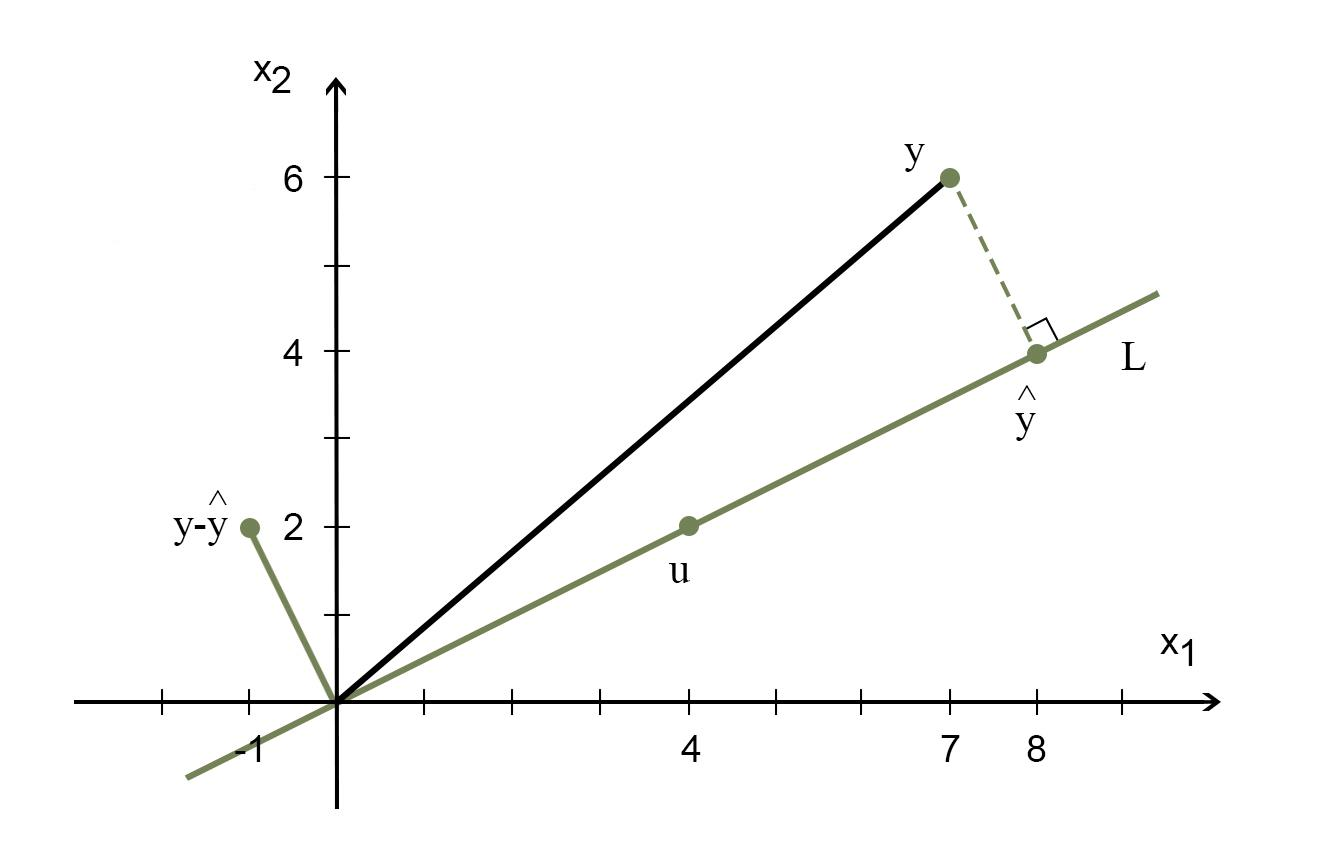
\includegraphics[width=0.80\textwidth]{Pictures/PROYvL.jpg}
    \caption{Proyección del vector $\vec{y}$ sobre la recta $L$. }
    \label{PROYORTOG}
\end{figure}

\begin{definition}
\bigskip
Sea $V$ un espacio vectorial  de dimensión finita con producto interno y sea $S\subseteq V$ un subespacio. Se define la \textit{proyección ortogonal } sobre $S$ como la transformación lineal $P_S :  V \rightarrow V$ que satisface 

\bigskip

\begin{enumerate}

\item $P_S(\vec{s})=\vec{s} $  $ ~ \forall \vec{s}\in S$

\bigskip

\item $P_S(\vec{t})=\vec{0} $  $ ~ \forall \vec{t}\in S^{\perp}$

\end{enumerate}

\end{definition}

\bigskip



\begin{example}
  En $\mathbb{R}^2$  se desea hallar la proyección ortogonal de un vector $\vec{y}$, $ \vec{\hat{y}}$  sobre el subespacio $S$  generado por otro vector $\vec{u} $, o sea sobre la recta $L$ generada por $\vec{u} $ que pasa por el origen. Esto se muestra en la Figura \ref{PROYORTOG}.

  $$P_S(\vec{y})= \vec{\hat{y}}= c \vec{u},$$ y se debe cumplir que $\vec{u} $ sea ortogonal al vector $ \vec{y} -\vec{\hat{y}}$, es decir, $ (\vec{y} -c \vec{u}) \cdot \vec{u}=0 $, entonces,
$$ \vec{y}  \cdot \vec{u} -c \vec{u} \cdot \vec{u}=0  $$
\noindent
  de donde 
  \[c= \frac{\vec{y}  \cdot \vec{u}}{\vec{u} \cdot \vec{u}}
  \]

\noindent
y entonces, la  proyección sobre $L$ es ,
  \begin{equation}
       \label{proyR2}
\vec{\hat{y}}=  \frac{\vec{y}  \cdot \vec{u}}{\vec{u} \cdot \vec{u}}\vec{u}
\end{equation}

  En el caso de la Figura \ref{PROYORTOG}, se tiene que 
  $ \vec{y}= \left(\begin{array}{c}  7  \\ 6
\end{array}
 \right)$  y $\vec{u}=   \left(\begin{array}{c}  4  \\ 2 
\end{array}
 \right).$
 
\bigskip

 Usando Ec.(\ref{proyR2}), como  $\vec{y}  \cdot \vec{u}=40$   y  $\vec{u}  \cdot \vec{u}=20$, se obtiene, 

\bigskip

\[\vec{\hat{y}}=  \frac{\vec{y}  \cdot \vec{u}}{\vec{u} \cdot \vec{u}}\vec{u}= \frac{40}{20}\vec{u}= 2 \vec{u}=\left(\begin{array}{c}  8  \\ 4
\end{array}
 \right)\]
\noindent
 y la componente ortogonal a $  \vec{u}$  es 
 $\vec{y}- \vec{\hat{y}} =\left(\begin{array}{c}  -1  \\ 2
\end{array}
 \right)   .$
 
\bigskip

 La descomposición de $\vec{y}$, como suma de proyecciones sobre $S$ y sobre  $S^{\perp}$, es

 

$$\left(\begin{array}{c}  7  \\ 6
\end{array}
 \right)=\left(\begin{array}{c}  8  \\ 4
\end{array}
 \right)+ \left(\begin{array}{c}  -1  \\ 2
\end{array}
 \right)$$
 
\end{example}

\bigskip

\begin{remark}
\begin{itemize}
    \item 
   Si $B=\left\{\vec{v}_1,\vec{v}_2,\cdots,\vec{v}_r,\vec{v}_{r+1}, \cdots\vec{v}_n\right\}$ una base ortonormal de $V$ tal que $\left\{\vec{v}_1,\vec{v}_2,\cdots,\vec{v}_r\right\}$ es una base de $S$ y $ \left\{\vec{v}_{r+1}, \cdots\vec{v}_n\right\}$ una base de $S^{\perp}$, la proyección ortogonal sobre $S$ es la única transformación lineal $P_S :  V \rightarrow V$ que satisface 

\bigskip

\begin{enumerate}

\item $P_S(\vec{v}_i)=\vec{v}_i $  $ ~ \forall ~ 1 \leq i \leq r$

\bigskip

\item $P_S(\vec{v}_i)=\vec{0} $  $ ~ \forall ~ r+1 \leq i \leq n$

\end{enumerate}

\bigskip

En consecuencia, para $\vec{v}\in V$, recordando que $ \vec{v} =\sum^{n}_{j=1}   (\vec{v}, \vec{v}_j)  \vec{v}_j $   resulta,


%\begin{equation}
% \label{formulaproy}   
%P_S(\vec{v})&= & P_S (\sum^{n}_{j=1}   (\vec{v}, \vec{v}_j)  \vec{v}_j ) \\ 
%P_S(\vec{v})&=& \sum^{n}_{j=1}   (\vec{v}, \vec{v}_j)  P_S (  \vec{v}_j )=\sum^{r}_{j=1}   (\vec{v}, \vec{v}_j)  \vec{v}_j  
%\end{equation}

\begin{equation}
 \label{formulaproy}   
P_S(\vec{v})=  P_S (\sum^{n}_{j=1}   (\vec{v}, \vec{v}_j)  \vec{v}_j )  = \sum^{n}_{j=1}   (\vec{v}, \vec{v}_j)  P_S (  \vec{v}_j )=\sum^{r}_{j=1}   (\vec{v}, \vec{v}_j)  \vec{v}_j,  
\end{equation}



\noindent
que es una expresión para $P_S(\vec{v})$ en términos de los vectores de la base ortonormal de $S$.
 \item
Sea $V$ un espacio vectorial  de dimensión finita con producto interno y sea $S\subseteq V$ un subespacio.
Entonces $P_S+P_{S^{\perp}}=id_V$,

\bigskip
\noindent
donde, 
 $P_S(\vec{v})= \sum^{r}_{j=1}   (\vec{v}, \vec{v}_j)  \vec{v}_j $  y $ ~P_{S^{\perp}}(\vec{v})=\sum^{n}_{j=r+1}   (\vec{v}, \vec{v}_j)  \vec{v}_j.$
    
\end{itemize}
%\hfill$\blacktriangle$
\end{remark}


\bigskip




\begin{example}

\end{example}
Si  $V=\mathbb{R}^4 $ y $W$ es el subespacio 

$$W= \left \{ \vec{x} \in \mathbb{R}^4,~ x_1-2x_2 + x_3= x_1-3x_2 +x_4=0  \right \},$$
se desea hallar la proyección ortogonal del vector $\vec{v}= (4,8,-4,12)$ sobre el subespacio $W$.
	
Para usar la expresión de la Ec.(\ref{formulaproy}) debemos hallar una base ortonormal de $W$.
 En primer lugar calculamos una base de $W$ resolviendo el sistema por eliminación
de Gauss:

\bigskip

\begin{equation}
 \left(\begin{array}{cccc} 1  & -2  & 1 & 0  \\ 1 & -3 & 0 & 1
\end{array}
 \right) \rightarrow  \left(\begin{array}{cccc} 1  & -2  & 1 & 0  \\ 0 & -1 & -1 & 1
\end{array}
 \right)
\end{equation}

\bigskip
A partir de la matriz escalonada, al resolver el sistema homogéneo,  quedan como variables independientes $x_3$ y $x_4$  y una base de $W$ es 

$\left \{ (-3,-1,1,0),(2,1,0,1) \right \}$.  Una base ortogonal,  de $W$ a partir de aplicar Gram-Smichdt  es 
$$  \left \{ (-3,-1,1,0),(\frac{1}{11},\frac{4}{11},\frac{7}{11},1) \right \}. $$ 



Si llamamos $\vec{w}_1=(-3,-1,1,0)$ y $\vec{w}_2=(\frac{1}{11},\frac{4}{11},\frac{7}{11},1)$, los vectores de la base ortonormal $\vec{v}_i$ se obtienen dividiéndolos por su norma, $\vec{v}_i =\frac {\vec{w}_i} {\left\| \vec{w}_i \right\|}.$ 


\bigskip


Entonces,  como $P_W(\vec{v})= \sum^{2}_{j=1}   (\vec{v}, \vec{v}_j)  \vec{v}_j  $, se calculan los productos escalares $(\vec{v}, \vec{v}_j)$, y se obtiene que  

$$P_W((4,8,-4,12))= (\frac{124}{17},\frac{88}{17}, \frac{52}{17}, \frac{140}{17}  )$$


\bigskip

\noindent
es el vector del subespacio  $W$ más cercano a $\vec{v}= (4,8,-4,12)$.


\end{example}

\bigskip

%Es interesante leer el teorema de la mejor aproximación  pag 398 Lay.

\begin{corollary}
    

 Teorema de la proyección ortogonal.
 \label{TPOr}

Sea $S$ un subespacio de un espacio vectorial con producto interno, $V$. Entonces, para cada $\vec{v} \in V$, el vector de $S$ a menor distancia de $\vec{v}$ es $P_S(\vec{v})$.

\begin{proof}



Si $B=\left\{\vec{v}_1,\vec{v}_2,\cdots,\vec{v}_r,\vec{v}_{r+1}, \cdots\vec{v}_n\right\}$ una base ortonormal de $V$ tal que $\left\{\vec{v}_1,\vec{v}_2,\cdots,\vec{v}_r\right\}$ es una base de $S$.

Sea $\vec{v} \in V$. Se tiene que $\vec{v}= \sum^{n}_{j=1}   (\vec{v}, \vec{v}_j)  \vec{v}_j $  y $ ~P_{S}(\vec{v})=\sum^{r}_{j=1}   (\vec{v}, \vec{v}_j)  \vec{v}_j $.
Por otro lado, si $\vec{s} \in S$, $\vec{s}= \sum^{r}_{j=1}   (\vec{s}, \vec{v}_j)  \vec{v}_j  $.


Entonces

$$\vec{v}-\vec{s}= \sum^{n}_{j=1}   (\vec{v}, \vec{v}_j)  \vec{v}_j -  \sum^{r}_{j=1}   (\vec{s}, \vec{v}_j)  \vec{v}_j = \sum^{r}_{j=1}   (\vec{v} - \vec{s}, \vec{v}_j)  \vec{v}_j+ \sum^{n}_{j=r+1}   (\vec{v}, \vec{v}_j)  \vec{v}_j  $$


\noindent
de donde,

$$\left\|\vec{v}-\vec{s}\right\|^2=  \sum^{r}_{j=1}   \left|(\vec{v} - \vec{s}, \vec{v}_j)\right|^2 + \sum^{n}_{j=r+1}  \left| (\vec{v}, \vec{v}_j) \right|^2  \geq    

\sum^{n}_{j=r+1}  \left| (\vec{v}, \vec{v}_j)\right|^2 = \left\|\vec{v}-P_{S}(\vec{v})\right\|^2 $$

\end{proof}

\end{corollary}

\bigskip

\begin{remark}
\begin{itemize}
    \item 
El teorema anterior es conocido también como el Teorema de la mejor aproximación.
\item
En la Figura \ref{PROYORTOG},  $\vec{\hat{y}}$ es el punto de $L$ más cercano a $\vec{y}$, en el sentido que
$$\left\|\vec{y}-\vec{\hat{y}}\right\| \leq \left\|\vec{y}-\vec{v} \right\|,$$
para todo $\vec{v}$ en $L$ distinto de $\vec{\hat{y}}$.
\end{itemize}
%\hfill$\blacktriangle$
\end{remark}


\bigskip

%Ver del LAY un ejemplo

\subsection{Problema de cuadrados mínimos}
El problema de hallar la proyección de  un vector $\textbf{b}$ sobre un subespacio surge cuando se tiene el problema $A\textbf{x}=\textbf{b}$, con $A$ una matriz de $m \times n$, donde $m$ es la cantidad de observaciones es mucho mayor que la cantidad de incógnitas $n$, de forma tal que se espera que el sistema $A\textbf{x}=\textbf{b}$ sea incompatible. En otras palabras, el vector $\textbf{b}$ no es combinación lineal de los vectores columna de $A$ (no está en el espacio columna de $A$). Se trata entonces, de hallar $ \hat x$ que minimice el error, y esto se realizará en el sentido de los cuadrados mínimos. El error es $E=\left\|Ax-\textbf{b}\right\|$, y es la distancia de $\textbf{b}$ al vector $A\textbf{x}$ en el espacio columna. El vector $\textbf{p}$ del espacio columna  más próximo a $\textbf{b}$ que cualquier otro es la \textit{proyección de $\textbf{b}$ sobre el espacio columna}. El error $Vec{e}=\textbf{b}-A  \hat{\textbf{x}}$ es perpendicular al espacio columna.
%(ver figura  pag 162 Strang).
Recordando que  el espacio nulo de la matriz $A$ es el conjunto de vectores de $\mathbb{R}^{n}$ que son perpendiculares a todas las filas de $A$, el error $\textbf{e}$ pertenecerá al espacio nulo de la matriz $A^T$ (es perpendicular al espacio columna). Es decir que el error Vec{e} es perpendicular a cada columna de $A$  (ver Figura \ref{MINCUAD_1}). Entonces se tiene que,


\begin{equation}
  A^T(\textbf{b}-A \hat{\textbf{x}})=0 \qquad  \text{o}  \qquad    A^TA  \hat{\textbf{x}}=A^T\textbf{b}
  \label{150}
\end{equation}

Las ecuaciones (\ref{150}) se conocen como \textit{ecuaciones normales}\index{Ecuaciones normales}. Pueden obtenerse a partir de buscar  $\textbf{x}$ que minimiza $E^2$, tomando derivadas parciales de $E^2= (Ax-b)^T(Ax-b)$. Al igualar a cero,   se tiene $2A^TA\textbf{x}-2A^T\textbf{b}=0$.


Si $A^TA$ tiene inversa (esto ocurre cuando las columnas de $A$ son linealmente independientes), entonces 

\begin{equation}
  \hat {\textbf{x}}=  (A^T A)^{-1}A^T\textbf{b}
  \label{160}
\end{equation}
y la proyección $\textbf{p}$ de $\textbf{b}$ sobre el espacio columna, es el vector $A \hat{\textbf{x}}$

\begin{equation}
  \textbf{p}= A \hat{\textbf{x}}= A (A^T A)^{-1}A^T \textbf{b}
  \label{170}
\end{equation}

\begin{figure}
    \centering
    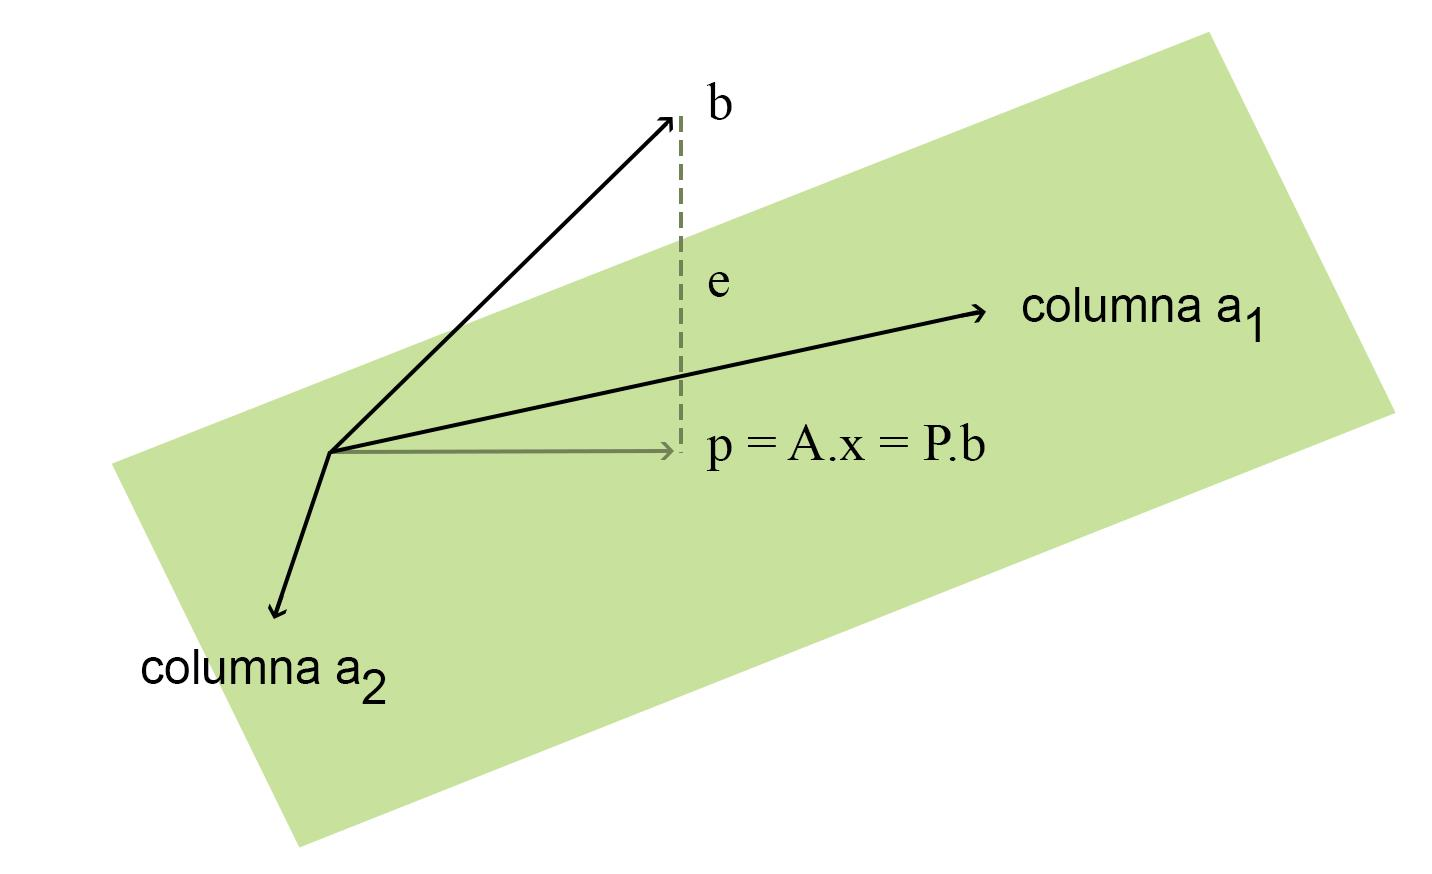
\includegraphics[width=0.80\textwidth]{Pictures/CUADM1.jpg}
    \caption{Proyección sobre el espacio columna.}
    \label{MINCUAD_1}
\end{figure}

\subsubsection{Un ejemplo de ajuste de datos  por  cuadrados mínimos}\index{Ajuste por cuadrados mínimos}

Supongamos realizamos un experimento en el que se espera que la salida $\textbf{b}$ sea una función lineal de la entrada $\textbf{t}$. Se buscará la recta $\textbf{b}= \alpha + \beta \textbf{t}$. Por ejemplo, si a diferentes tiempos medimos la distancia a un satélite en su recorrido a Marte. En este caso $\textbf{t}$ es el tiempo y $\textbf{b}$ la distancia y el satélite se moverá con una velocidad casi constante ($\textbf{b}=\textbf{b}_0 + v \textbf{t})$. 
¿Es posible calcular $\alpha$ y $\beta$ ? Si no hay errores experimentales dos mediciones determinan la recta $\textbf{b}= \alpha + \beta \textbf{t}$. Pero si hay error  se deberá promediar los experimentos y hallar la \textit{mejor} recta.
Al realizar $m$ mediciones, 

\begin{eqnarray*}
  \alpha + \beta t_1&=& b_1 \\
  \alpha + \beta t_2&=& b_2  \\
  \cdots  \\
  \alpha + \beta t_m&=& b_m
  \label{180}
\end{eqnarray*}

Se tendrá un sistema \textit{sobredeterminado}, con  $m$ ecuaciones y solo $2$ incógnitas. Si las mediciones tienen error, el sistema no tiene solución. En este caso la matriz $A$ tiene dos columnas  y $\textbf{x}=( \alpha, \beta)^T$:

\begin{eqnarray}
\left(\begin{array}{cc} 1 \quad t_1\\ 1  \quad t_2
\\  1  \quad t_3 \\ \cdots \\ 1  \quad t_m 
\end{array}\right) \left(\begin{array}{c} \alpha\\ \beta
\end{array}\right)= \left(\begin{array}{c} b_1\\ b_2
\\  b_3 \\ \cdots \\ b_m 
\end{array}\right)
\end{eqnarray}

o $A\textbf{x}=\textbf{b}$.
La mejor recta se tendrá con $\hat{\textbf{x}}= (\hat \alpha, \hat \beta)$ que minimizan 

$$E^2=\left\|A \textbf{x}-\textbf{b} \right\|^2= (b_1- \alpha- \beta t_1)^2 + (b_2- \alpha- \beta t_2)^2 +  \cdots (b_m- \alpha- \beta t_m)^2 $$.

El vector $\textbf{p}=A \hat{\textbf{x}}$ es el más cercano a $\textbf{b}$. De todas las rectas $\textbf{b}= \alpha + \beta \textbf{t}$ estamos eligiendo la que mejor ajusta los datos. 
%Ver figura (Strang  Figure 3.9). 
Los errores son las distancias verticales $\textbf{b}- \alpha - \beta t$ (no perpendiculares). Estas distancias verticales se elevan al cuadrado, se suman y se minimizan.



\bigskip


 
\begin{example}
    
\end{example}

Si se considera como ejemplo, que se tienen tres mediciones:
\noindent
$b_1=1$ en $t_1=-1$, $b_2=1$ en $t_2=1$  y $b_3=3$ en $t_3=2$ se tiene el sistema $Ax=b$

\begin{equation}
\left(\begin{array}{cc} 1 & -1  \\  1 &  1 \\  1 & 2 
\end{array}
 \right) \left(\begin{array}{c} \alpha \\  \beta 
\end{array}
 \right)=  \left(\begin{array}{c} 1    \\  1 \\  3
\end{array}
 \right)
 \label{190}
\end{equation}
 
 El sistema es incompatible porque los puntos no están sobre una misma recta. Se resuelve entonces, por cuadrados mínimos,
  $A^TA  \hat{\textbf{x}}=A^T\textbf{b}$
  
  \begin{equation}
\left(\begin{array}{cc} 3 & 2  \\  2 &  6 
\end{array}
 \right) \left(\begin{array}{c} \hat \alpha \\  \hat \beta 
\end{array}
 \right)=  \left(\begin{array}{c} 5    \\  6 
\end{array}
 \right)
 \label{200}
\end{equation}

\bigskip

La solución es $\hat \alpha= \frac{9}{7}$, $\hat \beta= \frac{4}{7}$ y la mejor recta es $ \frac{9}{7} + \frac{4}{7} t $.

\bigskip

Como se muestra  en la Figura \ref{MINCUAD_3}, el vector $\textbf{b}$ no es combinación lineal de las columnas $( 1,1,1)^T$ y $( -1,1,2)^T$. Con mínimos cuadrados se reemplaza $\textbf{b}$ que no está en la recta  por el vector $\textbf{p}=A \hat{\textbf{x}}$ que sí está, al no poder resolver $A\textbf{x}=\textbf{b}$, se resuelve $A \hat{\textbf{x}} = \textbf{p}$. El vector $\textbf{p}=( \frac{5}{7}, \frac{13}{7} ,\frac{17}{7}  )$  está en el espacio columna, es la proyección en ese subespacio. Restando $\textbf{p}$ de $\textbf{b}$, los errores son $\textbf{e}=\textbf{b}-\textbf{p}=( \frac{2}{7},  -\frac{6}{7}, \frac{4}{7} )$. Son los errores verticales en la Figura \ref{MINCUAD_2}. Ese vector $\textbf{e}$, como se muestra en la  Figura \ref{MINCUAD_3}, es ortogonal a las  columnas de $A$ (está en el espacio nulo de $A^T$).

\begin{figure}
    \centering
    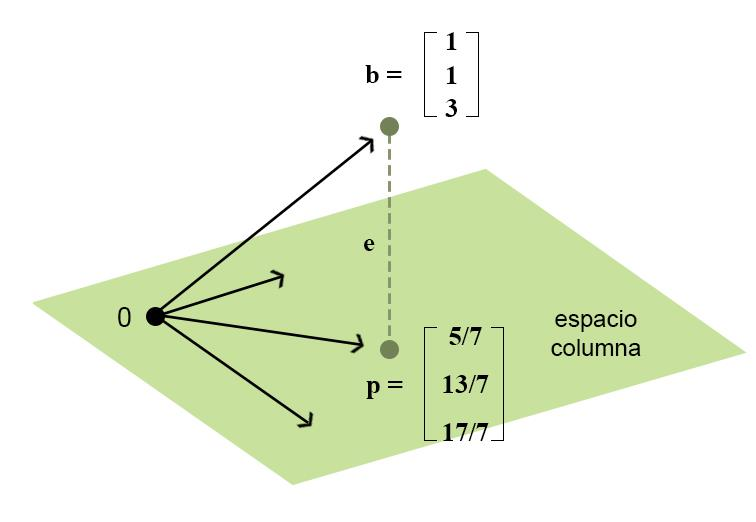
\includegraphics[width=0.80\textwidth]{Pictures/CUADM3.jpg}
    \caption{Proyección del vector $b$ en el espacio columna.}
    \label{MINCUAD_3}
\end{figure} 


\begin{figure}
    \centering
    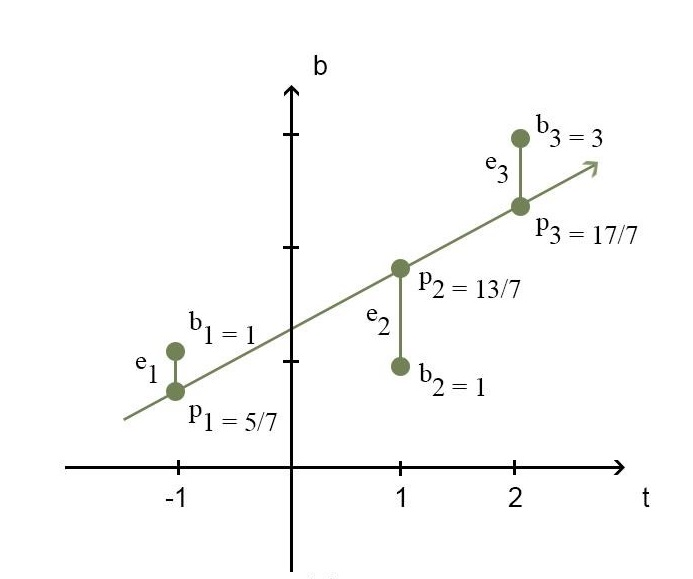
\includegraphics[width=0.75\textwidth]{Pictures/CUADM2.jpg}
    \caption{Recta que ajusta  por mínimos cuadrados los datos del ejemplo.}
    \label{MINCUAD_2}
\end{figure}
%\end{example}

Para el caso  de $m$ mediciones  $b_1, b_2,   \cdots, b_m$   en puntos  distintos $t_1, t_2,   \cdots, \\ t_m$, la recta  
$\alpha + \beta t$ que minimiza  $E^2$, surge de resolver el sistema lineal 

 \begin{equation}
A^TA\left(\begin{array}{c} \hat \alpha \\  \hat \beta 
\end{array}
 \right)= A^T b
 \label{210}
\end{equation}

o 

 \begin{equation}
\left(\begin{array}{cc} m & \sum_{i=1}^m t_i  \\  \sum_{i=1}^m t_i &  \sum_{i=1}^m t_i^2 
\end{array}
 \right) \left(\begin{array}{c} \hat \alpha \\  \hat \beta 
\end{array}
 \right)=  \left(\begin{array}{c} \sum_{i=1}^m b_i    \\ \sum_{i=1}^m t_i b_i
\end{array}
 \right)
 \label{220}
\end{equation}


 
  \bigskip
\begin{remark}  
Es importante notar que el método de cuadrados mínimos no está limitado a ajustar datos con una recta. En muchos casos interesan otros ajustes, con polinomios de grado más alto o con otras funciones como es el caso de ajuste  exponencial o el ajuste con senos y cosenos. Pueden conducir a problemas lineales o a problemas no lineales de cuadrados mínimos, siendo estos últimos  más complejos de abordar. 
\end{remark}


\begin{remark}
 El método por mínimos cuadrados fue inventado por Karl Friedrich Gauss, y lo usó para resolver un problema de astronomía. En 1801 el asteroide Ceres se había observado mucho más brillante durante más de un mes antes de desaparecer cuando se acercó al Sol. Con base en las observaciones disponibles, los astrónomos deseaban aproximar la órbita de Ceres para observarlo de nuevo cuando se alejara del sol. Gauss empleó los mínimos cuadrados e impactó a la comunidad científica al predecir la hora y el lugar correctos (unos 10 meses después) para localizar el asteroide.
 %\hfill$\blacktriangle$
\end{remark}


\index{Gauss, Karl Friedrich}
\begin{parchment}[Karl Friedrich Gauss (1777 - 1855)]{ Fue un matemático, astrónomo y físico alemán que contribuyó significativamente en muchos ámbitos, incluida la teoría de números, el análisis matemático, la geometría diferencial, la estadística, el álgebra, la geodesia, el magnetismo y la óptica. 

Gauss pronto fue reconocido como un niño prodigio, pese a provenir de una familia campesina de padres con poca cultura: su madre sabía leer, aunque no escribir; su padre sí, pero en cuanto a las matemáticas, no pasaba de la aritmética más elemental. De Carl Friedrich Gauss existen muchas anécdotas acerca de su asombrosa precocidad. Completó su magnum opus, Disquisitiones arithmeticae, a los veintiún años (1798), aunque la obra no se publicó hasta 1801. Constituye un trabajo fundamental como consolidación de la teoría de los números y ha moldeado esta área hasta los días presentes. \cite{gauss} }
\end{parchment} 


\section{Endomorfismos de espacios vectoriales con producto interno}\index{Endomorfismos}

Vamos a asociar ahora a cada endomorfismo  $f$ de un espacio vectorial $V$  de dimensión finita y con producto interno otra transformación lineal $f ^{*}$, $f ^{*}: V \rightarrow V  $.


\bigskip
\begin{definition}


Sea $V$ un espacio vectorial  con producto interno y sea $f$ una transformación lineal. Se llama \textit{adjunta} de $f$ y se anota  $f ^{*}$ a una transformación lineal $f ^{*}: V \rightarrow V  $ tal que 

 \begin{equation}
(f(\vec{v}),\vec{w})=(\vec{v},f ^{*}(\vec{w})) \qquad  \forall \vec{v},\vec{w}\in V
 \label{230}
\end{equation}
\end{definition}


\bigskip


\begin{example} 
\label{ejemplotadjunta}


Sea $f: \mathbb{C}^{2}\rightarrow  \mathbb{C}^{2}$ con el producto interno canónico, dada por 
$f(x,y)=((x+iy, 2x-(1+i)y)$


\bigskip


Se tiene que

\bigskip


% completar todos los pasos
$(f(x,y),(z,w))= ((x+iy, 2x-(1+i)y),(z,w) )= ((x,y), (z+2w,-iz+(-1+i)w))$ 

\bigskip
\noindent
de donde, $f ^{*}:  \mathbb{C}^{2}\rightarrow  \mathbb{C}^{2}  $ definida por $f ^{*}(z,w)=(z+2w, -iz+(-1+i)w)$ satisface 
$(f(x,y),(z,w))=((x,y),f ^{*}(z,w))$ para todo par de vectores $(x,y),(z,w)$ en $\mathbb{C}^{2}$.
\end{example}
\bigskip

  




El resultado que sigue prueba que  en espacios vectoriales   con producto interno de dimensión finita,   la transformación lineal adjunta existe y es única. 





\bigskip
\begin{theorem}

Sea $V$ un espacio vectorial de dimensión finita  con producto interno y sea $f$ una transformación lineal, $f: V \rightarrow V$. Entonces existe una única transformación lineal $f ^{*}: V \rightarrow V  $ tal que $$(f(\vec{v}),\vec{w})=(\vec{v},f ^{*}(\vec{w}))$$ 

\begin{proof}
Unicidad

Para ver la unicidad supongamos existen transformaciones lineales $g^{*}: V \rightarrow V$ y  $ h^{*}: V \rightarrow V $ tales que, para $\vec{w}$ fijo y para cada $\vec{v}$

$$ (f(\vec{v}), \vec{w})= (\vec{v},g(\vec{w}) )\qquad  (f(\vec{v}), \vec{w})= (\vec{v},h(\vec{w}))  $$
entonces 


$(\vec{v},g(\vec{w}))=(\vec{v},h(\vec{w}))$  o equivalentemente, $(\vec{v},g(\vec{w})-h(\vec{w}))=\vec{0}$, para todo $\vec{v} \in V$; tomando $ \vec{v}= g(\vec{w})-h(\vec{w})$, se tiene $(g(\vec{w})-h(\vec{w}),g(\vec{w})-h(\vec{w}))=0 $ y por la propiedad del producto escalar $g(\vec{w})-h(\vec{w})=0$, entonces $g(\vec{w})=h(\vec{w})$, para cada $\vec{w} \in V $, con lo cual $g$ y $h$ coinciden.

\bigskip

Existencia


Sea  $\left\{\vec{v}_1,\vec{v}_2, \cdots\vec{v}_n\right\}$ una base ortonormal de $V$. Si existe $f ^{*}: V \rightarrow V  $ con las condiciones del enunciado, debe cumplirse, para cada $\vec{w} \in V $


$$f ^{*}(\vec{w})= \sum_{i=1}^n (f ^{*}(\vec{w}), \vec{v}_i)\vec{v}_i$$

$$= \sum_{i=1}^n \overline{  ( \vec{v}_i,f ^{*}( w)})\vec{v}_i$$

$$ = \sum_{i=1}^n \overline{  (f(\vec{v}_i),\vec{w})}\vec{v}_i = \sum_{i=1}^n (\vec{w}, f(\vec{v}_i))\vec{v}_i  $$

Se define entonces, $f ^{*}: V \rightarrow V  $

\begin{equation}
  \label{adjunta}  
f ^{*}(\vec{w})= \sum_{i=1}^n (\vec{w},  f(\vec{v}_i))\vec{v}_i
\end{equation}

\bigskip

$f ^{*}$ es una transformación lineal


\begin{itemize}
     
    
    \item
    Usando la definición Ec.(\ref{adjunta} ),
    $$f ^{*}(\vec{w_1}+\vec{w_2} )=  \sum_{i=1}^n ( \vec{w_1}+\vec{w_2} ,  f(\vec{v}_i))\vec{v}_i $$
    
    $$=  \sum_{i=1}^n ( \vec{w_1} ,  f(\vec{v}_i)) + (\vec{w_2} ,  f(\vec{v}_i))\vec{v}_i $$
    
    $$=  \sum_{i=1}^n ( \vec{w_1} ,  f(\vec{v}_i))\vec{v}_i +  \sum_{i=1}^n (\vec{w_2} ,  f(\vec{v}_i))\vec{v}_i $$
    
    $$= f ^{*}(\vec{w_1} )+ f ^{*}(\vec{w_2} )$$
    
    \item
    
    
    Para $\lambda \in \mathbb{C} ($o$  \mathbb{R})$  $\vec{w} \in V$
    
    $$f ^{*}(\lambda \vec{w} )=  \sum_{i=1}^n ( \lambda \vec{w} ,  f(\vec{v}_i))\vec{v}_i $$
    
    $$ = \lambda \sum_{i=1}^n  (\vec{w} ,  f(\vec{v}_i))\vec{v}_i= \lambda f ^{*} (\vec{w})    $$
    
\end{itemize}

\bigskip


Veamos que para todo $ \vec{v},  \vec{w} \in V $ vale $(f(\vec{v}),\vec{w})=(\vec{v},f ^{*}(\vec{w}))$

\bigskip

Sean $ \vec{v},  \vec{w} \in V $. Se tiene que  $ \vec{v}= \sum_{i=1}^n ( \vec{v} ,  \vec{v}_i)\vec{v}_i $ y entonces, $ f(\vec{v})= \sum_{i=1}^n ( \vec{v} ,  \vec{v}_i)f(\vec{v}_i) $


$$ (f(\vec{v}),  \vec{w} )  = (\sum_{i=1}^n ( \vec{v} ,  \vec{v}_i)f(\vec{v}_i), \vec{w} )  $ $

$$  = \sum_{i=1}^n ( \vec{v} ,  \vec{v}_i)(f(\vec{v}_i), \vec{w} )   $$



Por otro lado 


$$( \vec{v},f ^{*}(\vec{w}))  =  (\sum_{i=1}^n ( \vec{v} ,  \vec{v}_i)\vec{v}_i),  \sum_{j=1}^n ( \vec{w} ,  f(\vec{v}_j))\vec{v}_j)     $$

$$  \sum_{i=1}^n ( \vec{v} ,  \vec{v}_i)(\vec{v}_i,  \sum_{j=1}^n ( \vec{w} ,  f(\vec{v}_j))\vec{v}_j)     $$

$$  \sum_{i=1}^n ( \vec{v} ,  \vec{v}_i)\sum_{j=1}^n  \overline{  ( \vec{w} ,  f(\vec{v}_j))  }( \vec{v}_i,  \vec{v}_j)$$  

$$\sum_{i=1}^n ( \vec{v} ,  \vec{v}_i) \overline{  ( \vec{w} ,  f(\vec{v}_i))  } = \sum_{i=1}^n ( \vec{v} ,  \vec{v}_i)  (  f(\vec{v}_i), \vec{w}  )   $$

\bigskip

Concluimos entonces que se cumple $(f(\vec{v}),\vec{w})=(\vec{v},f ^{*}(\vec{w}))$



\end{proof}
\end{theorem}




%COMPLETAR Unicidad. Existencia. 

%Se define $f ^{*}(\vec{w})= \sum^{n}_{i=1}(\vec{w},f(\vec{v}_i))\vec{v}_i$ , se prueba que es lineal y cumple lo pedido

\bigskip

\bigskip


A partir de la matriz de una transformación lineal $f: V \rightarrow V$ en una base ortonormal de $V$, puede obtenerse fácilmente la matriz de su adjunta en la misma base.


\bigskip


\begin{theorem}

Sea $V$ un espacio vectorial de dimensión finita  con producto interno y sea $f$ una transformación lineal, $f: V \rightarrow V$. Sea $B$ una base ortonormal de $V$. Entonces, la matriz que representa la transformación adjunta es la conjugada y transpuesta de la matriz de la transformación $f$, es decir,
\begin{equation}
(f^{*})_B= (( f )_B)^{*}
 \label{240}
\end{equation}



\bigskip

\begin{proof}

Supongamos que $B=\left\{\vec{v}_1,\vec{v}_2, \cdots\vec{v}_n\right\}$ es  una base ortonormal de $V$. Entonces para cada $1 \le i, j \le n$, 

$$((f^{*})_B)_{ij}= (f^{*}(\vec{v}_j), \vec{v}_i)$$
\noindent
como  en cada columna $j$ van las coordenadas de $f^{*}(\vec{v}_j$) en la base $B$,

$$=\overline{(\vec{v}_i, f^{*}(\vec{v}_j))}= \overline{(f(\vec{v}_i), \vec{v}_j)}= (\overline{( f )_B)})_{ji}= (( f )_B)^{*}_{ij} $$

\end{proof}

\end{theorem}

\bigskip

\bigskip

\begin{example}
En el caso de la transformación lineal adjunta del Ejemplo \ref{ejemplotadjunta}, si $B$ es la base canónica de $\mathbb{C}^{2}$, se tiene, de acuerdo a la proposición anterior, que la matriz que la representa es:

\bigskip

$(f)_B= \left(\begin{array}{cc}  1 & i  \\ 2 &  -1-i 
\end{array}
 \right)$  y   $ \qquad (f ^{*})_B= \left(\begin{array}{cc}  1 & 2  \\ -i &  -1+i 
\end{array}
 \right)$ \\
 
\noindent 
$(f ^{*})_B$ es la matriz transpuesta y conjugada de $(f)_B$.

  
\bigskip 


\end{example}



\bigskip

%Ver  propiedades del EH

Existe el caso particular de transformaciones lineales $f: V \rightarrow V$ cuya adjunta $f ^{*}$ coincide con $f$.

\bigskip

\begin{definition}\index{Transformación lineal autoadjunta} 

Sea $V$ un espacio vectorial  con producto interno y sea $f: V \rightarrow V$ una transformación lineal. Se dice que $f$ es \textit{autoadjunta}  si   $f= f ^{*}$ o sea, tal que


 \begin{equation}
(f(\vec{v}),\vec{w})=(\vec{v},f (\vec{w})) \qquad  \forall  ~ \vec{v}, \vec{w}\in V 
 \label{250}
\end{equation}
\end{definition}


\bigskip
\begin{definition}
 
Una matriz    $A \in \mathbb{R}^{n \times  n  }$   se dice \textit{simétrica} si $A _{ij}={A _{ji}}$    $\forall  1 \le i,j \le n$, o equivalentemente, si $A=A^T$. Una matriz  $A \in \mathbb{C}^{n \times  n  }$ se dice\textit{ hermitiana} si $A _{ij}=\overline {A _{ji}}$ $\forall  1 \le i,j \le n$, o equivalentemente, si $A=A^*$.  
\end{definition}
\bigskip

Si $A$ es la matriz de una transformación lineal $f$ en una base  ortonormal, sabemos que $A ^{*}$ es la matriz de la transformación adjunta en la misma base. Si $f$ es autoadjunta se tiene $A= A ^{*}$, por lo tanto la matriz de una transformación lineal autoadjunta es simétrica (hermítica).

%Ver propiedades de las autoadjuntas (p 385)









\bigskip

Si $f$ es autoadjunta, entonces, es una transformación lineal  diagonalizable. Más aún,  existe una base ortonormal de $V$ formada por autovectores de $f$ y todos sus autovalores son reales. 

\bigskip


\begin{theorem}

Sea $V$ un espacio vectorial  de dimensión finita con producto interno. Sea $f$ una transformación lineal autoadjunta. Entonces el polinomio característico de $f$ tiene todas sus raíces reales.

%\begin{proof}}
\end{theorem}
\bigskip

\begin{remark}
 Si $A \in \mathbb{C}^{n \times  n  }$ es una matriz hermitiana, entonces todas las raíces del polinomio característico de $A$ son reales.
 %\hfill$\blacktriangle$
\end{remark} 
 
\bigskip

El que sigue es un resultado importante sobre diagonalización de transformaciones lineales autoadjuntas.

\bigskip

\begin{theorem}
\label{diagreal}
Sea $V$ un espacio vectorial  de dimensión finita con producto interno. Sea $f: V \rightarrow V$ una transformación lineal autoadjunta. Entonces existe una base ortonormal $B$ de $V$  tal que la matriz $(f)_B$ es diagonal real.

\end{theorem}

\bigskip


\begin{remark}
 \begin{itemize}
     \item 
 Sea $A \in \mathbb{R}^{n \times  n  }$ es una matriz simétrica. Si se considera el producto interno canónico en $\mathbb{R}^{n}$, la transformación lineal $f_A: \mathbb{R}^{n}\rightarrow  \mathbb{R}^{n}$ definida por $f_A(\vec{x})=A\vec{x}$ es autoadjunta. Por la Proposición \ref{diagreal}  existe una base ortonormal $B$ de $\mathbb{R}^{n}$ tal que $(f_A )_B=D$, donde $D$ es una diagonal real. En este caso, si $E$ es la base canónica de $\mathbb{R}^{n}$, $(f_A )_E=A$,  $D= (P_{BE})^{-1}A(P_{BE})$, y  $(P_{BE})^{-1}=(P_{BE})^{t}$.
\item 
Análogamente, si    $A \in \mathbb{C}^{n \times  n  }$  es una matriz hermitiana. Si se considera $\mathbb{C}^{n}$ con   el producto interno canónico, la transformación lineal $f_A: \mathbb{C}^{n}\rightarrow  \mathbb{C}^{n}$,  definida por $f_A(\vec{x})=A\vec{x}$ es autoadjunta, y si $E$ es la base canónica de $\mathbb{C}^{n}$, $(f_A )_E=A$.
Por la proposición anterior  existe una base ortonormal $B$ de $\mathbb{C}^{n}$ tal que $(f_A )_B=D$, donde $D$ es una diagonal real. 
Entonces $ (P_{E,B})^{-1}A(P_{E,B})$, donde, por lo anterior $(P_{E,B})^{-1}=(P_{E,B})^{*}$.
% REVISAR SI $P_{BE}$   es la matriz de cambio de base de $B$ a $E$.
\end{itemize}
%\hfill$\blacktriangle$
\end{remark} 
\bigskip




Esto anterior nos lleva a la siguiente definición

\bigskip

\begin{definition}\index{Matriz ortogonal}\index{Matriz unitaria} 
\label{Matriz ortogonal}
Una matriz $O$ se dice \textit{ortogonal } si es invertible y $O^{-1}=O^{t}$.
Una matriz $U\in \mathbb{C}^{n \times  n  }$ se dice \textit{unitaria } si  es invertible y $U^{-1}=U^{*}$.
\end{definition} 


\begin{example}
Dada la matriz $A$,

\begin{equation}
A= \left(\begin{array}{cc} 1 & 1-i  \\ 1+i & 0
\end{array}
 \right), 
\end{equation}
se desea hallar una matriz unitaria $U$ tal que $U^{*}AU$  sea diagonal
\end{example}
Si en el programa Octave escribimos $[U,D]= eig(A)$
\noindent
nos devuelve las matrices $U$ y $D$ (con edición de $4$  dígitos):


\begin{equation}
U= \left(\begin{array}{cc} 0.4082-0.4082i & 0.5774-0.5774i  \\ -0.8165 & 0.5774
\end{array}
 \right), \qquad  D= \left(\begin{array}{cc} -1 & 0  \\ 0 & 2
\end{array}
 \right)
\end{equation}

\bigskip

Se verifican $U^{*}U=I$ y $U^{*}AU=D$


\bigskip

\bigskip

Resumiendo


\begin{enumerate}

\item  Sea   $A \in \mathbb{R}^{n \times  n  }$  una matriz simétrica. Entonces existe una matriz ortogonal  $O\in \mathbb{R}^{n \times  n  }$ tal que 
$O^{t}AO$ es diagonal.

%(En el Grossman está la demostración. Es el Teorema 3 del Capítulo 6, sección 4.)


\item Sea   $A \in \mathbb{C}^{n \times  n  }$ una matriz hermitiana. Entonces existe una matriz unitaria $C\in \mathbb{C}^{n \times  n  }$ tal que 
$C^{*}AC$ es diagonal real.


\end{enumerate}


\bigskip


\begin{remark}
    Toda transformación lineal autoadjunta en un espacio euclídeo de dimensión finita tiene sus autovalores reales
\end{remark}
\bigskip

%\begin{theom}
%(Diagonalización de matrices simétricas (hermíticas))
%La matriz de una transformación lineal autoadjunta puede ser reducida en una base ortonormal determinada %a una matriz diagonal.

%\end{theom}

\begin{example}

Se quiere diagonalizar ortogonalmente la matriz \index{Diagonalización}

\begin{equation}
A= \left(\begin{array}{cc} 1 & -2  \\ -2 & 3
\end{array}
 \right), \label{300}
\end{equation}

\bigskip


La ecuación característica de $A$ es $det(a- \lambda I)=  \left |\begin{array}{cc} 1-  \lambda & -2  \\ -2 & 3-\lambda  
\end{array}
 \right |= \lambda ^2 - 4 \lambda -1=0  $.
 
\bigskip
Tiene dos raíces, $\lambda_1= 2-\sqrt 5$  y  $\lambda_2= 2+\sqrt 5$


\bigskip


\noindent 
y los vectores propios correspondientes, son $ \vec{v}_1=  \left (\begin{array}{c} 2  \\ -1 + \sqrt 5  
\end{array}
 \right )$  y $ \vec{v}_2=  \left (\begin{array}{c} 1 - \sqrt 5   \\  2
\end{array}
 \right )$.
 
\bigskip

 %Notar que $\vec{v}_1. \vec{v}_2   =0$  (son ortogonales por teorema XX).
 
Para obtener vectores ortonormales los dividimos por su longitud, entonces,


\bigskip

$ \vec{u}_1= \frac{1}{\sqrt{10-2\sqrt 5}} \left (\begin{array}{c} 2  \\ -1 + \sqrt 5  
\end{array}
 \right )$ y  $ \vec{u}_2= \frac{1}{\sqrt{10-2\sqrt 5}} \left (\begin{array}{c} 1 - \sqrt 5   \\  2  
\end{array}
 \right )$

\begin{equation}
O= \frac{1}{\sqrt{10-2\sqrt 5}} \left(\begin{array}{cc} 2 & 1 - \sqrt 5 \\ -1 + \sqrt 5 & 2
\end{array}
 \right), \label{310}
\end{equation}

\bigskip

y $O^T A O =\left(\begin{array}{cc} 2-\sqrt 5 & 0  \\ 0 & 2+\sqrt 5
\end{array}
 \right)  $ 

\end{example}

\bigskip


\bigskip

\begin{example}



Sea 

\begin{equation}
A= \left(\begin{array}{cc} 2 & 3-3i  \\ 3+3i  & 5
\end{array}
 \right), \label{3000}
\end{equation}

\noindent
 una matriz hermitiana $\in \mathbb{C}^{2 \times 2}$.

 \bigskip
Es posible  diagonalizarla con la matriz unitaria 
 
\begin{equation}
U= \frac{1}{\sqrt{3}} \left(\begin{array}{cc} -1+i & 1 \\ 1 & 1+i
\end{array}
 \right), \label{320}
\end{equation}

\bigskip
\noindent
y se tiene que  $U^* A U =\left(\begin{array}{cc} -1 & 0  \\ 0 & 8
\end{array}
 \right)  $ 
es una matriz diagonal real.

\end{example}

\bigskip


\subsubsection{Transformaciones ortogonales}\index{Transformación ortogonal}
\label{Transf.Ortogonales}
Veremos ahora endomorfismos de un espacio vectorial con producto interno que preservan el producto interno y en particular, las distancias entre vectores.

\bigskip

\begin{theorem}

Sea $V$ un espacio euclídeo. Una transformación lineal $f$  se llama ortogonal si 
$(f(\vec{v}),f(\vec{w}))=(\vec{v},\vec{w})$ $~\forall \vec{v},\vec{w} \in V$. Es decir $f$ conserva el producto escalar.
\end{theorem}


\bigskip

\begin{theorem}
Toda transformación lineal $f$ en un espacio euclídeo  que conserve la longitud de los vectores  es una transformación ortogonal.

\begin{proof} 

$$\left\|f(\vec{v}+\vec{w})\right\|^{2}=   (f(\vec{v}+\vec{w}),f(\vec{v}+\vec{w})) $$

$$=\left\|f(\vec{v})\right\|^{2}  +2   (f(\vec{v}),f(\vec{w})) +  \left\|f(\vec{w})\right\|^{2} $$

\bigskip

\noindent
y, por otro lado, 

$$\left\|\vec{v}+\vec{w}   \right\|^{2} =   \left\|\vec{v}\right\|^{2} +2   (\vec{v},\vec{w}) +  \left\|\vec{w}\right\|^{2} $$

\bigskip

Como $f$ conserva la longitud de los vectores, $\left\|f(\vec{v}+\vec{w})\right\|=\left\|\vec{v}+\vec{w}\right\|$, $\left\|f(\vec{v})\right\|=\left\|\vec{v}\right\|$, $\left\|f(\vec{w})\right\|=\left\|\vec{w}\right\|$, entonces, igualando términos en las expresiones anteriores, se tiene que, 

\bigskip
$$(f(\vec{v}),f(\vec{w}))=(\vec{v},\vec{w}),$$

\noindent
y se  prueba que $f$ es ortogonal.

\end{proof} 
\end{theorem}

\bigskip

   \begin{example}
  
  $f=id_V$  es una transformación lineal ortogonal
\end{example} 

\bigskip


\begin{example} 
  
  
  Una rotación en $\mathbb{R}^{2}$ (con centro en el origen de coordenadas) es una transformación lineal ortogonal.
  
  Ya vimos en la Sección \ref{MatrizdeunaTL},  (Ec.(\ref{rot})) que la matriz de una  rotación en un ángulo $\theta$ en sentido antihorario, respecto de una base ortonormal es 
  
  \begin{equation}
R_{\theta}= \left(\begin{array}{cc} cos(\theta)   & -sen(\theta) \\ sen(\theta) & cos(\theta)
\end{array}
 \right), \label{400}
\end{equation}

\bigskip

Se verifica  que   $\forall \vec{v} \in \mathbb{R}^{2}  $,  $ \left\|R \vec{v}\right\|^{2} =  \left\|\vec{v}\right\|^{2}$
   \end{example} 
   
\bigskip
  
\begin{example}
  En $\mathbb{R}^{2}$ cualquier simetría con respecto a un subespacio vectorial unidimensional es una transformación lineal ortogonal.  
  
  
  En el caso de simetría respecto del eje $x$, en la base canónica, la matriz es 
  
  
  \begin{equation}
S= \left(\begin{array}{cc} 1   & 0\\ 0 & -1
\end{array}
 \right), \label{500}
\end{equation}



\end{example} 
  
\begin{remark}
\begin{itemize}
     \item 
     En $\mathbb{R}^{2}$ las únicas transformaciones ortogonales son las rotaciones y las simetrías, mientras que en
     $\mathbb{R}^{3}$ hay más  posibilidades de tener transformaciones lineales ortogonales que en $\mathbb{R}^{2}$.
\item
Para estudiar todas las posibles transformaciones lineales ortogonales se deben analizar los autovalores.
\item
Puede demostrarse que toda transformación lineal $f$ que transforma al menos una base ortonormal en una base ortonormal, es ortogonal.
\end{itemize}
\end{remark}

\bigskip


 \begin{example} 
En $\mathbb{R}^{3}$ la simetría con respecto a una recta, como se muestra  en la  Figura  \ref{SIM_3}.
La matriz de la transformación en la base $\{ \vec{u}_1, \vec{u}_2, \vec{u}_3  \}$ es 
%(ver Hernández figuras pág. 393).

\bigskip


$$\left(\begin{array}{ccc} 1  & 0  & 0  \\ 0 & -1 & 0  \\ 0 & 0 & -1
\end{array}
 \right)$$
\end{example} 

\begin{figure}
    \centering
    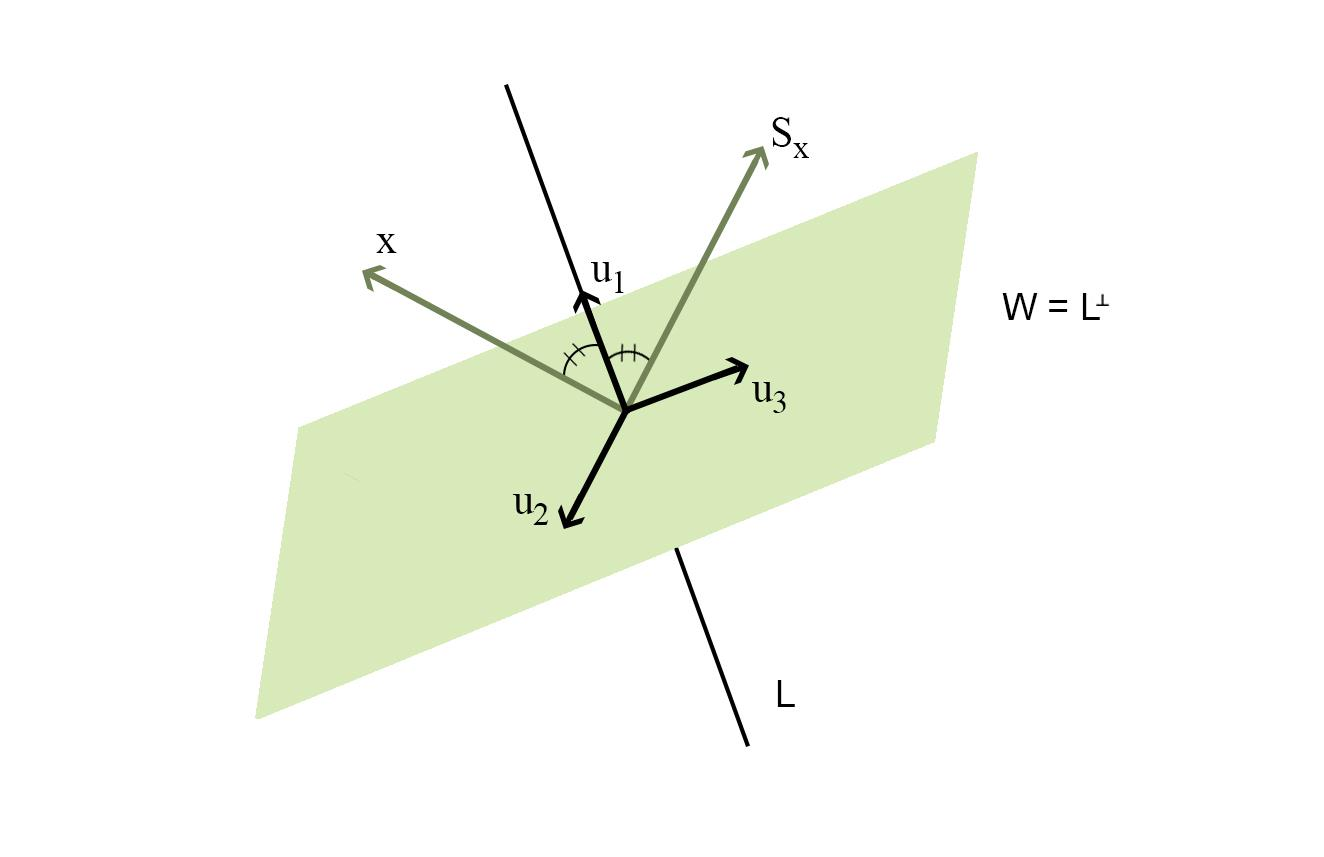
\includegraphics[width=0.80\textwidth]{Pictures/fig.32.jpg}
    \caption{Simetría con respecto a una recta.}
    \label{SIM_3}
\end{figure} 


\bigskip

 



\bigskip

\begin{theorem}
\label{det1ortog}

Los autovalores reales de una  transformación lineal ortogonal son iguales a $1$ o a $-1$.


\begin{proof}

Si $\lambda$ es un autovalor real de una transformación ortogonal, con autovector  $\vec{v}$, se tiene

$$(\vec{v},\vec{v})=(f(\vec{v}),f(\vec{v}))= ( \lambda \vec{v}, \lambda \vec{v})= \lambda ^2 (\vec{v},\vec{v})$$

Por lo tanto $ \lambda ^2 = 1$  y $ \lambda  = +- 1$. 

  \end{proof}
  \end{theorem}
\bigskip


\begin{remark} \index{Descomposición espectral de una matriz}
\begin{itemize}
    \item 

Una transformación lineal que cumple las  condiciones anteriores se dice unitaria  si $V$ es un $\mathbb{C}$ espacio vectorial y ortogonal si $V$ es un   $\mathbb{R}$ espacio vectorial.

\bigskip

$ f$ es unitaria (ortogonal) $\longleftrightarrow$  $(f)_B$ es unitaria (ortogonal) 

\bigskip

\item

Cuando A es simétrica y no demasiado grande, los algoritmos de computadora modernos que se usan  actualmente calculan con gran precisión vectores y valores propios.
Esos algoritmos aplican a $A$ una sucesión de transformaciones de semejanza en las
que intervienen matrices ortogonales.  El uso de matrices ortogonales evita que
los errores numéricos se acumulen durante el proceso. Cuando A es simétrica, la
sucesión de matrices ortogonales se combina para formar una matriz ortogonal cuyas
columnas son vectores propios de $A$.
Una matriz no simétrica no puede tener un conjunto completo de vectores propios
ortogonales, por lo que se necesitan técnicas no ortogonales para calcular los vectores
propios.


\bigskip

\item
Cuando una matriz $A$ tiene $n$ vectores propios ortogonales se llama \textit{descomposición espectral} de $A$ a la expresión

$$A= \lambda_1 \vec{u}_1^t \vec{u}_1 +\lambda_2 \vec{u}_2^t \vec{u}_2 + \cdots +\lambda_n \vec{u}_n^t \vec{u}_n.$$

La matriz $A$ queda dividida en partes determinadas por el espectro, y cada término es una matriz de rango $1$. Entre las aplicaciones de esta descomposición está la compresión de imágenes, que se realiza considerando  $k$ términos en lugar de $n$, con $k <n $, 
\end{itemize}
%\hfill$\blacktriangle$
\end{remark} 

\bigskip
%
%\end{document}

\newpage

%\begin{figure}
    %\centering
    %
\includegraphics[width=0.60\textwidth]{Pictures/prodint.png}    
    %\label{TLfig12}
%\end{figure}



\section{Actividades propuestas}
\begin{answers}

De acuerdo con la segunda ley de Kepler, un cometa debería tener una órbita elíptica,\index{Orbita de un cometa} parábolica o hiperbólica (despreciando las atracciones gravitacionales de los planetas). En convenientes coordenadas polares, la posición (r,$\vartheta$) de un cometa satisface una ecuación de la forma:

$$r=\beta+ e(r.\cos(\vartheta))$$

\noindent
donde $\beta$ es una constante y $e$ es la excentricidad de la órbita (con $0\leq e \le 1$ para una elipse,
e=1 para una parábola, y $e\ge 1$ para una hipérbola).
Suponga que los siguientes datos corresponden a las observaciones de un cometa recién descubierto. 

\bigskip

\begin{table*}[ht]
	\centering
					\begin{tabular}{lccccc}
\hline\hline
$\vartheta$&0.88&1.10&1.42&1.77&2.14\\
\hline
r &3.00&2.30&1.65&1.25&1.01\\
		\end{tabular}
\end{table*}
Determine el tipo de órbita e indique dónde estará el cometa cuando $\vartheta$=4.6 radianes.

\bigskip

\end{answers}

\bigskip

 \subsection{Ejercicios}
 
 \bigskip
%\subsubsection{Espacios Vectoriales con Producto Interno.}
 
 
\begin{exercise}
\item
Sea $\mathbb{E}$ un espacio euclídeo, si $\vec{x},\vec{y}$ y $\vec{z}$ son vectores de $\mathbb{E}$, desarrolle la siguiente expresión: ($\vec{x} +\vec{z}, \vec{x}-\vec{z}+\vec{y}$)
\end{exercise}
\begin{exercise}
\item

Calcule la distancia entre los vectores $\vec{u}=(2,i,1-i)$ y $\vec{v}=(-i,0,4i)$ en  $\mathbb{C}^3$ con el producto interno canónico. 
\end{exercise}


\begin{exercise}
\item

Pruebe que las siguientes  funciones definen productos internos sobre los espacios vectoriales considerados


a)   $  (\cdot,\cdot)$: $ C\left[0,1\right] \times C\left[0,1\right]  \rightarrow  \mathbb{R}, (f(x),g(x))= \int_0^1f(x)g(x)dx$.

b)   $   (\cdot,\cdot)$:  $K^{n \times n}  \times K^{n \times n}\rightarrow K$,(A,B)=$tr(A.B^*)$, con $K=\mathbb{R}$ y $K=\mathbb{C}$ ($B^*$ es la matriz traspuesta conjugada de B). 
\end{exercise}

\begin{exercise} 
\item

Determine para qué valores de $\alpha \in \mathbb{R} $:
\[
\phi((x_1,x_2),(y_1,y_2))=x_1y_1-x_1y_2-x_2y_1+\alpha x_2y_2
\]
es un producto interno en $\mathbb{R}^2$.
\end{exercise}
\begin{exercise}
\item

Sean $\vec{u}_1=(-2,-1,1),\vec{u}_2=(0,-1,0)$ y $\vec{u}_3=(1,-1,0)$ tres vectores linealmente independientes de $\mathbb{R}^3$. Si definimos el producto
escalar en $\mathbb{R}^3$ afirmando que $\{\vec{u}_1,\vec{u}_2,\vec{u}_3\}$ es una base ortonormal. ¿Cuál sería la expresión analítica de este producto escalar
en la base canónica de $\mathbb{R}^3$?

\end{exercise}


\bigskip

%\subsubsection{Matrices ortogonales y complemento ortogonal}

\vspace{0.25cm}

\begin{exercise}
\item
Demuestre que $Q$  $\in \mathbb{R}^{2 \times  2  }$ es una matriz de rotación puesto que $Q$ es ortogonal y además su determinante vale $1$.
$Q=\left(\begin{array}{cc}\cos(\phi) & -\sin(\phi) \\ \sin(\phi)& \cos(\phi)
\end{array}
 \right)$
\end{exercise}
\begin{exercise}

\bigskip

\item
En $P^{(2)}_{\mathbb{R}}\left[x\right]$ se define el producto escalar:
$\phi(p(x),q(x))= \int_{-1}^1p(x)q(x)dx$

\noindent Pruebe que el conjunto $\left\{1,x, \frac{1}{3}(3x^2 -1)\right\}$ es ortogonal.
\end{exercise}

\begin{exercise}
\item

Dada la matriz simétrica 
$A=\left(\begin{array}{cc}1 & -2 \\-2 & 1
\end{array}
 \right)$
 construya una matriz ortonormal $T$ tal que $(T^{-1}AT)$ sea una matriz diagonal. Verifique
 también que  $T^{-1}=T^{t}$ y que el determinante de $T$ es igual a 1. Obtenga asimismo la matriz
 diagonal $(T^{-1}AT)$.
\end{exercise}

%\newpage

\begin{exercise}
\item

Halle una base ortogonal de $\mathbb{R}^3$ -con el producto interno canónico- que contenga al vector $\vec{u}=(1,-1,2)$.
\end{exercise}
\begin{exercise}
\item
Sea 
\[A=\left(\begin{array}{ccc}1 & -2 & 0   \\ -2& 2 & -2
\\ 0  & -2 & 3                         
\end{array}
 \right)
\]

a) Halle una base ortonormal de autovectores de $A$.

b) Halle una matriz $P$ ortogonal tal que $P^tAP$ sea diagonal.
\end{exercise}
\begin{exercise}
\item


Sea $B=\{(1,0,1),(2,0,1),(1,1,0)\}$ una base de $\mathbb{R}^3$. Considere el producto interno canónico y utilice Gram-Schmidt para hallar a partir de $B$ una base $B^{\prime}$ que sea ortonormal. Calcule las coordenadas de $\vec{v}=(2,-1,3)$ en la base $B\prime$. Utilice sus resultados para encontrar la factorización $A=QR$.  Puede chequear sus resultados utilizando el diguiente programa Python:

\bigskip

\begin{lstlisting}[language = python, numbers = none, escapechar = !,
    basicstyle = \ttfamily\bfseries, linewidth = 1\linewidth] 
import numpy as np
# Definimos la matriz
A = np.array([[4, 3, 1],
              [2, 1, 3],
              [1, 1, 1]])
# Realizamos la descomposición QR
Q, R = np.linalg.qr(A)
# Imprimimos las matrices Q y R
print("Matriz Q:")
print(Q)
print("Matriz R:")
print(R)
\end{lstlisting}

\end{exercise}
\begin{exercise}
\item
Demuestre que S=$\left\{\vec{u}_1,\vec{u}_2,\vec{u}_3\right\}$ es un conjunto ortogonal donde

\bigskip


$\vec{u}_1=\left(\begin{array}{c} 3   \\ 1\\ 1                           
\end{array}
 \right) ,\vec{u}_2=\left(\begin{array}{c} -1   \\ 2\\ 1                           
\end{array}
 \right), \vec{u}_3=\left(\begin{array}{c} -\frac{1}{2}  \\ -2\\ \frac{7}{2}                       
\end{array} \right), \vec{y}=\left(\begin{array}{c} 6   \\ 1\\ -8                           
\end{array} \right)$


\bigskip

\noindent Exprese el vector $\vec{y}$
como combinación lineal del conjunto S. Recuerde las coordenadas se calculan cómo $c_j= (\frac{\vec{y}.\vec{u_j}}{\vec{u_j}\vec{u_j}})$ con $j=1,2,3$ por ser ortogonal.

\bigskip

\end{exercise}
\begin{exercise}
\item
Calcule la distancia de un punto $\vec{y}$ en $\mathbb{R}^3$ a un subespacio W generado por $\left\{\vec{u}_1,\vec{u}_2\right\}$ sabiendo que el punto más cercano se calcula como $\left\|\vec{y}-\hat{y}\right\|$, donde $\hat{y}=proy_w \vec{y}$.

\bigskip

$\vec{y}=\left(\begin{array}{c} -1   \\ -5\\ 10                           
\end{array}
 \right),\ vec{u}_1=\left(\begin{array}{c} 5   \\ -2\\ -1                           
\end{array}
 \right),\ vec{u}_2=\left(\begin{array}{c} 1   \\ 2\\ -1                          
\end{array} \right)$
\end{exercise}

\begin{exercise}
\item

Halle el complemento ortogonal para el siguiente subespacios de $V$:

$V=\mathbb{R}^3$, $S_1=\{(x_1,x_2,x_3)\in \mathbb{R}^3,  2x_1-x_2=0\} $ para el producto interno canónico.

\end{exercise}


\begin{exercise}
\item

Demuestre que el conjunto $S=  \{   cos nx,sen mx \}_{n,m \in  \mathbb{N}}$  es linealmente independiente en $C([0, 2 \pi])$.
Sugerencia: observar que 



$$\int_0^{2\pi}  (cos^2 nx )dx \neq 0, \quad   \int_0^{2\pi}  (sen^2 mx )dx \neq 0, \quad  n,m \in  \mathbb{N} $$ 

y 

$$\int_0^{2\pi}  (cos nx )(cos mx) dx =  \quad   \int_0^{2\pi}  (cos nx )(sen mx)) dx = 

=\quad  \int_0^{2\pi}  (sen nx )(sen mx) dx=0 $

\bigskip

si $n \neq m, n, m  \in  \mathbb{N} $ 

\bigskip

\end{exercise}


\newpage
 
%\subsubsection{Operador Adjunto. Operador Unitario }

\begin{exercise}
\item

Halle $T^*$ para cada una de las transformaciones lineales siguientes:

a) $T:\mathbb{R}^2 \rightarrow \mathbb{R}^2$, $T((x_1,x_2))=(3x_1+x_2,-x_1+x_2)$.\\

b) $T:\mathbb{R}^3 \rightarrow \mathbb{R}^3$, tal que $\left[T \right]_B=\left(\begin{array}{ccc}1 & 0 & 1   \\ 2& 0 & -1
\\ 0  & 1 & 0                         
\end{array}
 \right)$, 
 
 donde $B=\{(1,2,-1),(1,0,0),(0,1,1)\}$.

 \bigskip
 
 
%c)  $T:P^{(2)}_{\mathbb{R}}[x] \rightarrow P^{(2)}_{\mathbb{R}}[x]$, $T(p)=p'$, $(f,g)= \int_0^1f(x)g(x)dx$.

\end{exercise}

\begin{exercise}
\item
Determine si los siguientes endomorfismos definidos sobre $\mathbb{R}^3$ son autoadjuntos:

a) $T((x,y,z))=(x+y,x,-z)$

b) $S((x,y,z))=(-2x+2z,y,2x)$
\end{exercise}

\begin{exercise}
\item 

Encuentre en cada caso una matriz $O \in \mathbb{R}^{n \times n}$  ortogonal tal que $O.A.O^t$ sea diagonal

\bigskip

a) $A=\left(\begin{array}{cc}1 &  3   \\ 3 & -1
                       
\end{array}
 \right)$

\bigskip

b) $A=\left(\begin{array}{ccc}5 & 0 & -2   \\ 0 & 7 & -2
\\ -2  & -2 & 6                         
\end{array}
 \right)$

 
 

\end{exercise}

\newpage

\begin{exercise}
\item 


Dada 
$A=\left(\begin{array}{cccc}4 &1 & i & 0    \\ 1 & 3 & 2i
&0 \\ -i  & -2i & 3  & i \\0 & 1 &-i & 2                         
\end{array}
 \right)$

 \bigskip
 

\noindent encuentre una matriz $U \in \mathbb{C}^{n \times n}$  ortogonal tal que $U.A.U^*$ sea diagonal.
\end{exercise}
\begin{exercise}
\item

Halle la matriz en la base canónica de las siguientes transformaciones ortogonales

a)  $T:\mathbb{R}^2 \rightarrow \mathbb{R}^2$, rotación de un ángulo de $\frac {\pi}{4}$.


b)  $T:\mathbb{R}^2 \rightarrow \mathbb{R}^2$, simetría respecto de la recta $x_1=x_2$.

\end{exercise}

\bigskip

% \subsection{Ejercicios teóricos}\\
 
 \bigskip

\begin{exercise} 
\item

Sea $V$ un espacio vectorial y sea $(\cdot,\cdot)$ un producto interno sobre $V$. Pruebe

a) $( \Vec{x}, \Vec{y}+\Vec{z})= ( \Vec{x}, \Vec{y} ) +( \Vec{x}, \Vec{z} )$


b) $( \Vec{x}, c\Vec{y} )= \overline c ( \Vec{x}, \Vec{y} )$

c) $( \Vec{x}, \Vec{y})=  (\Vec{x},\Vec{z} )  \quad  \forall \Vec{x} \in V  \Rightarrow \Vec{y}=\Vec{z}$
\end{exercise}

\begin{exercise}
\item 


Sea $V$ un espacio vectorial con producto interno   $(\cdot,\cdot)$. Pruebe que $\left|(\Vec{x}, \Vec{y} )\right| =\left\|\Vec{x}\right\|\left\|\Vec{y}\right\|$ sí y sólo sí $\{\Vec{x},\Vec{y}\}$ es un conjunto linealmente dependiente.
\end{exercise}
\begin{exercise}
\item
Pruebe que dos vectores $\vec{x}$ e $\vec{y}$  son ortogonales, si 

$\left\|\vec{x}+\vec{y}\right\|^{2}=\left\|\vec{x}\right\|^{2}+\left\|\vec{y}\right\|^{2}$
\end{exercise}
%\newpage

\begin{exercise}
\item

Sea  $V$ un espacio vectorial sobre $K$ de dimensión finita con producto interno  $(\cdot,\cdot)$. Sea $T \in L(V)$ biyectivo. Considerar la aplicación    $(\cdot,\cdot)_{T}: V \times V \rightarrow  K$, $(\vec{x}, \vec{y})_{T} =( T(\vec{x}) ,T(\vec{y}))$, $~\forall \vec{x}, \vec{y} \in V$

\noindent Pruebe que $(\cdot,\cdot)_{T}$ también es un producto interno sobre $V$.
\end{exercise}
\begin{exercise}
\item

Sea $A \in   \mathbb{R}^{2 \times 2}$. Sea $\phi: \mathbb{R}^2 \times \mathbb{R}^2 \rightarrow \mathbb{R}$ definida por $\phi(x,y)=y.A.x^t$. Pruebe  que $\phi$ es un producto interno sobre $\mathbb{R}^2$ si y sólo sí $A=A^t$, $\~A_{11} \geq 0$ y $Det(A) \geq 0$.

\end{exercise}

\begin{exercise}
\item


Sea $V$ un $\mathbb{C}$-espacio vectorial con producto interno  $(\cdot,\cdot)$ y sea $T \in L(V)$ sobre $\mathbb{C}$. Pruebe que si $\lambda$ es autovalor  de $T$,  entonces  $\overline \lambda$ es un autovalor de $T^*$.
\end{exercise}

\begin{exercise}
\item


Sea $V$ un $\mathbb{C}$-espacio vectorial con producto interno  $(\cdot,\cdot)$ y sea $T \in L(V)$ sobre $\mathbb{C}$ autoadjunto. Pruebe que:


a)  si $\lambda$ es autovalor  de $T$,  entonces  $\lambda  \in \mathbb{R}$.

b) Si $v_i$ es autovector asociado al autovalor $\lambda_i$ de $T$ (para $i=1$,$2$) y $\lambda_1 \neq \lambda_2$, entonces
$(\vec{v_1}, \Vec{v_2})=0$.

\end{exercise}
\begin{exercise}
\item

Sea V un espacio vectorial de dimensión finita con producto interno y sean $S$ y $T$ $\in L(V)$. Si $k \in K$, pruebe:

a) $(S+T)^*=S^*+T^*$

b) $(kT)^*=\overline k T^*$

c)  $(ST)^*=T^*S^*$
\end{exercise}




\bigskip
 

 \subsection{Autoevaluación}
 \label{Auto4}
 \bigskip



\subsubsection{Verdadero o Falso.}


\bigskip

\begin{enumerate}
  

\item
El subespacio imagen de una transformación lineal es ortogonal a su núcleo.

\item
El vector cero es ortogonal a todo vector en $\mathbb{R}^n$.

\item
Sean W un plano a travéz del origen en $\mathbb{R}^3$ y L la recta que pasa por el origen y es perpendicular a W. Entonces $L^{\bot}=W$ y $W^{\bot}=L$.
\item
$T(\vec{x})=(\frac{\vec{x}.\vec{v}}{\vec{v}\vec{v}}).\vec{v}$ es una transformación de proyección.
\item
Una matriz cuadrada U tal que $U^{-1}=U^t$ se denomina ortogonal.
\item
Si $U$ es ortonormal tanto las filas como las columnas de U son ortonormales.
\item
En la factorización $QR$ el hecho de que R sea invertible es consecuencia directa de que las columnas de A sean linealmente independientes.
\item
Si $\left\{\vec{v}_1,\vec{v}_2,\vec{v}_3\right\}$ es una base ortogonal para W, entonces la multiplicación de $\vec{v}_3$ por un escalar, da una nueva base ortogonal  $\left\{\vec{v}_1,\vec{v}_2,3\vec{v}_3\right\}$
\item
Si $A=QR$, donde $Q$ tiene columnas ortonormales, entonces R=$Q^t A$.
\item
Si $\vec{x}$ no esta en un subespacio W, entonces $\vec{x}-proy_w \vec{x}$ no es cero.
\item
Un espacio vectorial con un producto escalar se dice que es un espacio vectorial euclídeo.
\item
Si $Q$ es ortogonal se cumple que la norma de $\vec{x}$ es igual a la norma de $Q\vec{x}$.
\item
Todo conjunto ortogonal de un espacio euclídeo es linealmente dependiente. 
\item
El determinante de una matriz ortogonal es $1$ ó $-1$.
\item
El producto de dos matrices ortogonales es la matriz identidad. 
\item
El rango de $A$ es $n$ si y sólo si $A^t=A$ es invertible.
\item
Descomponer un vector $\vec{y}$ en una suma de proyecciones ortogonales sobre espacios unidimensionales es la esencia del proceso de Gram-Smith.
\item
dim V = dim W + dim $W^{\bot}$.
\item
$d(\vec{u},-\vec{v})^2$= $\left\|\vec{u}+\vec{v}\right\|^2= \left\|\vec{u}\right\|^2 + \left\|\vec{v}\right\|^2 + 2\vec{u}\vec{v}$.



\end{enumerate}

\bigskip

%\begin{lstlisting}[language = python, numbers = none, escapechar = !,
%    basicstyle = \ttfamily\bfseries, linewidth = 1\linewidth] 
%import numpy as np
%a = np.random.randn(9, 6)
%q, r = np.linalg.qr(a)
%print(a)
%np.allclose(a, np.dot(q, r))  # a does equal qr
%r2 = np.linalg.qr(a, mode='r')
%np.allclose(r, r2)  # mode='r' returns the same r as mode='full'
%a = np.random.normal(size=(3, 2, 2)) # Stack of 2 x 2 matrices as input
%q, r = np.linalg.qr(a)
%print('matriz q')
%q.shape
%r.shape
%c=np.allclose(a, np.matmul(q, r))
%\end{lstlisting}

\bigskip

\chapterimage{Pictures/blue_space(1).jpg}

\chapter{Formas bilineales y cuadráticas}

En este capítulo  se dará una breve introducción al tema enfocada a
mostrar  aplicaciones de lo diagonalización de las matrices de las formas bilineales y cuadráticas  en el estudio  de secciones cónicas y superficies cuádricas. . 




\section{Formas bilineales y cuadráticas}

La ecuación general de una cónica está dada por una ecuación de segundo grado de la forma
\begin{equation}
a_{11}x_1^{2}+a_{12}x_1x_2+a_{22}x_2^{2}+ a_1 x_1 + a_2 x_2 + a = 0, \label{fcuadratica0}
\end{equation}
donde $a_{ij}$, $a_i$ ($i,j=1,2$) y $a$ son números reales  y al menos uno de los números $a_{ij}$ no es cero.
La parte principal es:



\begin{equation}
a_{11}x^{2}+a_{12}xy+a_{22}y^{2}
\end{equation}
\noindent
y puede escribirse

\begin{equation}
P(x,y)=a_{11}x^{2}+a_{12}xy+a_{22}y^{2}=(x, y) ~A \left(\begin{array}{c} x \\  y 
 \end{array}\right), \label{fcuadratica01}
\end{equation}


\bigskip
\noindent
donde $A$ es la matriz simétrica,
\begin{equation}
A= \left(\begin{array}{cc} a_{11} & a_{12}/2  \\a_{12}/2 & a_{22}
\end{array}
 \right). \label{fcmatriz}
\end{equation}

\bigskip



Y su generalización a $\mathbb{R}^{n}$, dado $\vec{x}=(x_1, x_2, x_3, \cdots, x_n) \in$ $\mathbb{R}^{n}$, es 



\begin{equation}
\label{fcuadratica01Rn}
P(\vec{x})=(x_1, x_2, x_3, \cdots, x_n)A \left(\begin{array}{c}  x_{1} \\  x_{2}  
\\  x_3 \\ \cdots \\  x_{n} 
\end{array}\right)
\end{equation}

\bigskip

\bigskip

\noindent
donde  $A$ es una matriz  simétrica $\in$ $\mathbb{R}^{n \times n}.$

\noindent
Análogamente al caso $n=2$, para $n=3$ se obtienen superficies de segundo grado.

\bigskip

Los dos ejemplos anteriores corresponden a   \textit{formas cuadráticas} (en $\mathbb{R}^{2}$ y en  $\mathbb{R}^{n}$), y son casos particulares de \textit{formas bilineales}, las que se definen a continuación.

\bigskip

\begin{definition}\textbf{Forma bilineal}\index{Forma bilineal}


Sea $V$ un espacio vectorial sobre $\mathbb{R}$ o $\mathbb{C}$. Una aplicación $\mathbf{A}:  V \times V\rightarrow \mathbb{R}$ (o $\mathbb{C}$) se dice que es una \textit{forma bilineal} sí y solo sí satisface:

\bigskip

\begin{enumerate}



\item  

$\mathbf{A}(\vec{x}+\vec{z},\vec{y}   )=\mathbf{A}(\vec{x},\vec{y}) + \mathbf{A}(\vec{z},\vec{y})$, $~ \forall~$  $\vec{x}$, $\vec{y}$, $\vec{z} $ $\in V$
\bigskip


\item $\mathbf{A}(\alpha\vec{x},\vec{y})=\alpha \mathbf{A} (\vec{x},\vec{y})$ $~ \forall~$$\vec{x}$, $\vec{y}$ $\in V$ y $~ \forall~$ $\alpha \in \mathbb{R} $ o $\mathbb{C}$

\bigskip


\item $\mathbf{A}(\vec{x},\vec{y} +\vec{z}  )=\mathbf{A}(\vec{x},\vec{y}) + \mathbf{A}(\vec{x},\vec{z})$, $~ \forall~$ $\vec{x}$, $\vec{y}$, $\vec{z} $ $\in V$

\bigskip


\item  $\mathbf{A}(\vec{x},\beta \vec{y})= \beta \mathbf{A}(\vec{x}, \vec{y})$ $~ \forall~$ $\vec{x}$, $\vec{y}$ y $~ \forall~$ $\beta \in \mathbb{R} $ o $\mathbb{C}$

\end{enumerate}


\end{definition}

\bigskip

\bigskip

\begin{remark}
Los productos internos reales son formas bilineales.
\end{remark}

\bigskip

\bigskip


\begin{example}
$\mathbb{E}$ un espacio  Euclídeo de dimensión finita, y $T$ una aplicación lineal de $\mathbb{E}$ en $\mathbb{E}$. Puede demostrarse que  $\mathbf{A}(\vec{x},\vec{y})=(\vec{x}, T \vec{y})$ es una forma bilineal.
\end{example}

\bigskip

\begin{example} 
Dados 

$\vec{x}=(x_1, x_2, x_3, \cdots, x_n)$ e $\vec{y}=(y_1, y_2, y_3, \cdots, y_n) \in$ $\mathbb{R}^{n}$,

$$P(\vec{x})=(x_1, x_2, x_3, \cdots, x_n)A \left(\begin{array}{c}  y_{1} \\  y_{2}  
\\  y_3 \\ \cdots \\  y_{n} 
\end{array}\right)$$

\noindent
donde  $A$ es una matriz  simétrica $\in$ $\mathbb{R}^{n \times n}$, es una forma bilineal.


\bigskip

La forma cuadrática en $\mathbb{R}^{n}$ de la Ec.(\ref{fcuadratica01Rn}) presentada antes sale de tomar para estee caso $\vec{x}=\vec{y}$.
\end{example}

\bigskip



\bigskip

\begin{remark}
\begin{itemize}
    \item 

Una forma bilineal se dice \textit{simétrica} si  $A(\vec{x},\vec{y})= A(\vec{y},\vec{x})$

\item 

Una forma bilineal se dice \textit{ antisimétrica} si  $A(\vec{x},\vec{y})= -A(\vec{y},\vec{x})$
\end{itemize}
\end{remark}

\bigskip

\begin{definition}\textbf{Matriz de una forma bilineal} \index{Matriz de una forma bilineal}

\bigskip

Sea  $\mathbf{A}$ una forma bilineal en un espacio $V$ y sea $B= \left\{\vec{e}_1,\vec{e}_2,\cdots, \vec{e}_n\right\}$ una base de $V$.


\bigskip

Si $\vec{x}=\sum^{n}_{i=1}x_i \vec{e}_i$, e $\vec{y}=\sum^{n}_{j=1}y_j \vec{e}_j$,


\begin{eqnarray*}
\mathbf{A}(\vec{x},\vec{y})&= &\mathbf{A} (\sum^{n}_{i=1} x_i \vec{e}_i, \sum^{n}_{j=1} y_j \vec{e}_j) \\
  &=&\sum^{n}_{i=1}\sum^{n}_{j=1} x_i y_j \mathbf{A}(\vec{e}_i, \vec{e}_j)
  \end{eqnarray*}


 Se define  la matriz de la forma bilineal $\mathbf{A}$ en la base $B$ como la matriz  $A \in \mathbb{R }^{n \times n }$    tal que $A_ {ij}= \mathbf{A}(\vec{e}_i,\vec{e}_j)$ para $1\leq i,j\leq n$
\end{definition}



\newpage






\begin{remark}
\begin{itemize}
    \item 
    
    Si $\mathbf{A}(\vec{x},\vec{y})= \mathbf{A}(\vec{y},\vec{x})$ (es decir $\mathbf{A}$ es una forma bilineal simétrica), entonces 
$\mathbf{A}(\vec{e}_i,\vec{e}_j) = \mathbf{A}(\vec{e}_j,\vec{e}_i)$   para cualquier base  $\left\{\vec{e}_1,\vec{e}_2,\cdots, \vec{e}_n\right\}$ de $V$, es decir la matriz de una forma bilineal $A$ simétrica en cualquier base es simétrica. 
Vale también la recíproca: si la matriz de una forma bilineal es simétrica en alguna base 
$\left\{\vec{e}_1,\vec{e}_2,\cdots, \vec{e}_n\right\}$ de $V$, entonces la forma bilineal es simétrica, pues

\bigskip


\begin{eqnarray*}
\mathbf{A}(\vec{y},\vec{x})&=& \sum^{n}_{i,j=1} \mathbf{A}(\vec{e}_i,\vec{e}_j) y_i x_j   \\
&= &\sum^{n}_{i,j=1} a_{ij} y_i x_j   \\
&=& \sum^{n}_{i,j=1} a_{ji}  x_j y_i \\
&= &\sum^{n}_{i,j=1} \mathbf{A}(\vec{e}_j,\vec{e}_i)  x_j y_i   \\
&=& \mathbf{A}(\vec{x},\vec{y})
\end{eqnarray*}

\bigskip

\item

%bolasazules{

\bigskip
Si $\mathbf{A}$ es una forma bilineal antisimétrica, $\mathbf{A}(\vec{x},\vec{y})= -\mathbf{A}(\vec{y},\vec{x})$ para cualquier base $\left\{\vec{e}_1,\vec{e}_2,\cdots, \vec{e}_n\right\}$ de $V$. La matriz satisface $a_{ij}=-a_{ji}$, de donde $a_{ii}=0$, $i=1,   \cdots , n$.

\bigskip

\item


Si $A$ es la matriz de una forma bilineal respecto a la base  $B= \left\{\vec{e}_1,\vec{e}_2,\cdots, \vec{e}_n\right\}$ y $\tilde{A}$ con respecto a la base $\tilde{B}= \left\{\vec{u}_1,\vec{u}_2,\cdots, \vec{u}_n\right\}$, entonces $A= C^{T} \tilde{A}C$, donde $C$ es la matriz de cambio de base de $B$ a $\tilde{B}$. Tienen el mismo rango $\tilde{A}$ y $ A $, ya que $det(C) \neq 0$.

\bigskip

\item
El rango de una forma bilineal es el rango que tiene la matriz de la forma bilineal en cualquier base.

\end{itemize}

\end{remark}


\bigskip



\begin{theorem}

Toda forma bilineal puede ser representada como la suma de una forma bilineal simétrica y una forma bilineal  antisimétrica.

\bigskip

\begin{proof}
Sea $\mathbf{A}$ una forma bilineal definida en $V$ y sea $\mathbf{B}:  V \times V\rightarrow K$  definida así $$\mathbf{B}(\vec{x},\vec{y})=\mathbf{A}(\vec{x},\vec{y})+\mathbf{A}(\vec{y},\vec{x})$$
y sea $\mathbf{C}:  V \times V\rightarrow K$
$$\mathbf{C}(\vec{x},\vec{y})=\mathbf{A}(\vec{x},\vec{y})-\mathbf{A}(\vec{y},\vec{x})$$


\bigskip

$$2\mathbf{A}(\vec{x},\vec{y})=\mathbf{B}(\vec{x},\vec{y})+ \mathbf{C}(\vec{x},\vec{y})$$

\vskip.3cm

$$\mathbf{A}(\vec{x},\vec{y})= \frac{\mathbf{B}(\vec{x},\vec{y})}{2}+ \frac{\mathbf{C}(\vec{x},\vec{y})}{2}$$


\noindent
donde 

$$\mathbf{B}(\vec{y},\vec{x})=\mathbf{A}(\vec{y},\vec{x})+ \mathbf{A}(\vec{x},\vec{y})=\mathbf{B}(\vec{x},\vec{y})$$


$$\mathbf{C}(\vec{y},\vec{x})=\mathbf{A}(\vec{y},\vec{x})- \mathbf{A}(\vec{x},\vec{y})=-\mathbf{C}(\vec{x},\vec{y})$$

\bigskip

Esto es similar a lo que ocurre con una matriz $A$, que puede expresarse, 
$$A= \frac{A+A^T}{2}+ \frac{A-A^T}{2}$$
\noindent
donde   $\frac{A+A^T}{2}$   es simétrica y $\frac{A-A^T}{2}$ antisimétrica.

\end{proof}
\end{theorem}


\begin{definition} \textbf{Forma cuadrática} \index{Forma cuadrática}

\bigskip


Dada  $\mathbf{A}$ $:  V \times V\rightarrow \mathbb{R}$  una forma bilineal,  se define una \textit{forma cuadrática }

  $\mathbf{Q} :   V\rightarrow \mathbb{R}$, $\mathbf{Q}(\vec{x})=\mathbf{A}(\vec{x},\vec{x})$.

\end{definition}

\bigskip


\begin{example}
$$\mathbf{Q}(x_1,x_2)=a_{11}x_1^{2}+a_{12}x_1x_2+a_{22}x_2^{2}$$
\end{example}



Usando la matriz $P$  definida antes, Ec.(\ref{fcuadratica01}) una forma cuadrática se escribe,






$$\mathbf{Q}(\vec{x})=(x_1, x_2, x_3, \cdots, x_n)P  (x_1, x_2, x_3, \cdots, x_n) ^{T}.$$
%\end{array}\right)$$


\bigskip

En general, toda expresión de la forma

$$\mathbf{Q}(\vec{x})=\sum^{n}_{j=1} \sum^{n}_{i \le j }  a_{ij} x_i x_j$$


\bigskip


\noindent
en un espacio vectorial define una forma cuadrática, ya que alcanza con tomar la forma bilineal 
  
\[
\mathbf{A}(\vec{x},\vec{y})= \sum^{n}_{i=1} a_{ii} x_i y_i  + \sum^{n}_{j=1} \sum^{n}_{i \le j } \frac{a_{ij}}{2} x_i y_j +  \sum^{n}_{j=1} \sum^{n}_{i  > j } \frac{a_{ij}}{2}  x_j y_i  
\]

  

    
  
con   $\vec{x}= \sum^{n}_{i=1}  x_i \vec{e}_i$ e  $\vec{y}= \sum^{n}_{j=1}  y_j \vec{e}_j$.

%\end{document}


 \bigskip


 \bigskip
 
\begin{remark}
Un ejemplo de forma bilineal   es el tensor de inercia,$I(\vec{x}, \vec{y})$ pero gran parte de su interés
radica en que $I(\omega, \omega)$ da la energía de rotacíon cuando la velocidad angular es $\omega$.
\end{remark}

 \bigskip

 
\subsection{Formas cuadráticas. Aplicación a las secciones cónicas}\index{Secciones cónicas}\index{Cuadrática}


La Ec.(\ref{fcuadratica0}) se reescribe, 

$$\mathbf{Q}(x_1,x_2)=a_{11}x_1^{2}+a_{12}x_1x_2+a_{22}x_2^{2}$$


\noindent
y también  en forma matricial,
\begin{equation}
\left(\begin{array}{cc}x_1 & x_2
\end{array}
 \right) \left(\begin{array}{cc} a_{11} & a_{12}/2  \\a_{12}/2 & a_{22}
\end{array}
 \right)  \left(\begin{array}{c} x_1 \\  x_2
\end{array}
 \right)+ \left(\begin{array}{cc}a_1 & a_2
\end{array}
 \right) \left(\begin{array}{c} x_1 \\ x_2
\end{array}
 \right) +a=0\label{fcuadraticatoda}
\end{equation}

\bigskip

\begin{equation}
\bf x ^T A \bf x + K \bf x + a =0 \label{fcuadraticamatricial}
\end{equation}
\noindent
donde 
\begin{equation}
\bf x=  \left(\begin{array}{c} x \\y
\end{array}
 \right),\qquad K=\left(\begin{array}{cc}a_1 & a_2
\end{array}
 \right)\label{fcuadraticaxyk}
\end{equation}
\index{Matriz de la forma cuadrática} 
Con esta notación, la forma cuadrática asociada a la Ec.(\ref{fcuadraticamatricial}) es $ \bf x ^T A \bf x$. La matriz simétrica $A$ se denomina \textit{matriz de la forma cuadrática } $ \bf x ^T A \bf x$. 

\bigskip

\begin{example}


En la ecuación,

\begin{equation}
3x_1^{2}+5x_1x_2-7x_2^{2}+ 2 x_1 + 7 = 0, \label{ejemplo61}
\end{equation}
la matriz de la forma cuadrática es, 

\bigskip

$\left(\begin{array}{cc}3 & 5/2 \\ 5/2 & 7
\end{array}
 \right)$.
 
 \bigskip
 
\noindent
mientras que para  la ecuación

\begin{equation}
8x_1^{2}-4x_2^{2} = 0, \label{ejemplo61}
\end{equation}
la matriz de la forma cuadrática es, 

\bigskip

$\left(\begin{array}{cc}8 & 0 \\ 0 & -4
\end{array}
 \right)$.

\end{example}

 \bigskip
 
 Para una cónica  $C$  con ecuación (\ref{fcuadraticamatricial})  es posible hacer girar los ejes de coordenadas $x_1x_2$ de modo que la ecuación de la cónica, en el sistema de coordenadas $x_1^\prime x_2^\prime$, no tenga término con producto cruzado.  
 
 \begin{itemize}
 
 \item
 Se halla una matriz $O$ que diagonaliza ortogonalmente a $A$, $A=ODO^t$. Se intercambian sus columnas en el caso que el $Det(O)\neq 1 $ para asegurar que la transformación de coordenadas sea una rotación.
 
 $$\bold x=O \bold x'$$
 
  \item
  Para obtener la ecuación en el sistema $x_1^\prime x_2^\prime$  se sustituye la ecuación anterior  en la Ec.(\ref{fcuadraticamatricial}).
 
 \begin{equation}
\bf (x^\prime) ^t O^t A O \bf x^\prime  + K O \bf x^\prime + a =0 \label{fcuadraticamatricialprima}
\end{equation}
Como $O$ diagonaliza ortogonalmente a la matriz $A$, $O^t A O =\left(\begin{array}{cc} \lambda_1 & 0 \\ 0 & \lambda_2
\end{array}
 \right)$,
 donde $\lambda_1$   y  $\lambda_2$  son los autovalores de $A$. Por lo tanto, la ecuación  (\ref{fcuadraticamatricialprima}) reescribir como
 
 \begin{equation}
\left(\begin{array}{cc}x_1^\prime & x_2^\prime
\end{array}
 \right) \left(\begin{array}{cc} \lambda_1& 0  \\ 0 & \lambda_2
\end{array}
 \right)  \left(\begin{array}{c} x_1^\prime \\x_2^\prime
\end{array}
 \right)+ \left(\begin{array}{cc}a_1 & a_2
\end{array}
 \right)
 \left(\begin{array}{cc} o_{11} & o_{12}  \\ o_{21} & o_{22}
\end{array}
 \right) 
 \left(\begin{array}{c} x_1^\prime \\x_2^\prime
\end{array}
 \right) +a=0\label{fcuadraticatoda}
\end{equation}
 o bien 
 
 $$\lambda_1(x^\prime_1)^{2}+\lambda_2(x^\prime_2)^{2}  +a_1^\prime x_1^\prime+ a_2^\prime x_2^\prime +a  =0$$

 \bigskip
 
 \noindent
 donde $a_1'=a_1o_{11}+a_2o_{21}$  y $a_2'=a_1o_{12}+a_2o_{22}$. 
 %Ahora la ecuación no tiene término de producto cruzado. 
 
  \end{itemize}
  
\begin{figure}
    \centering
    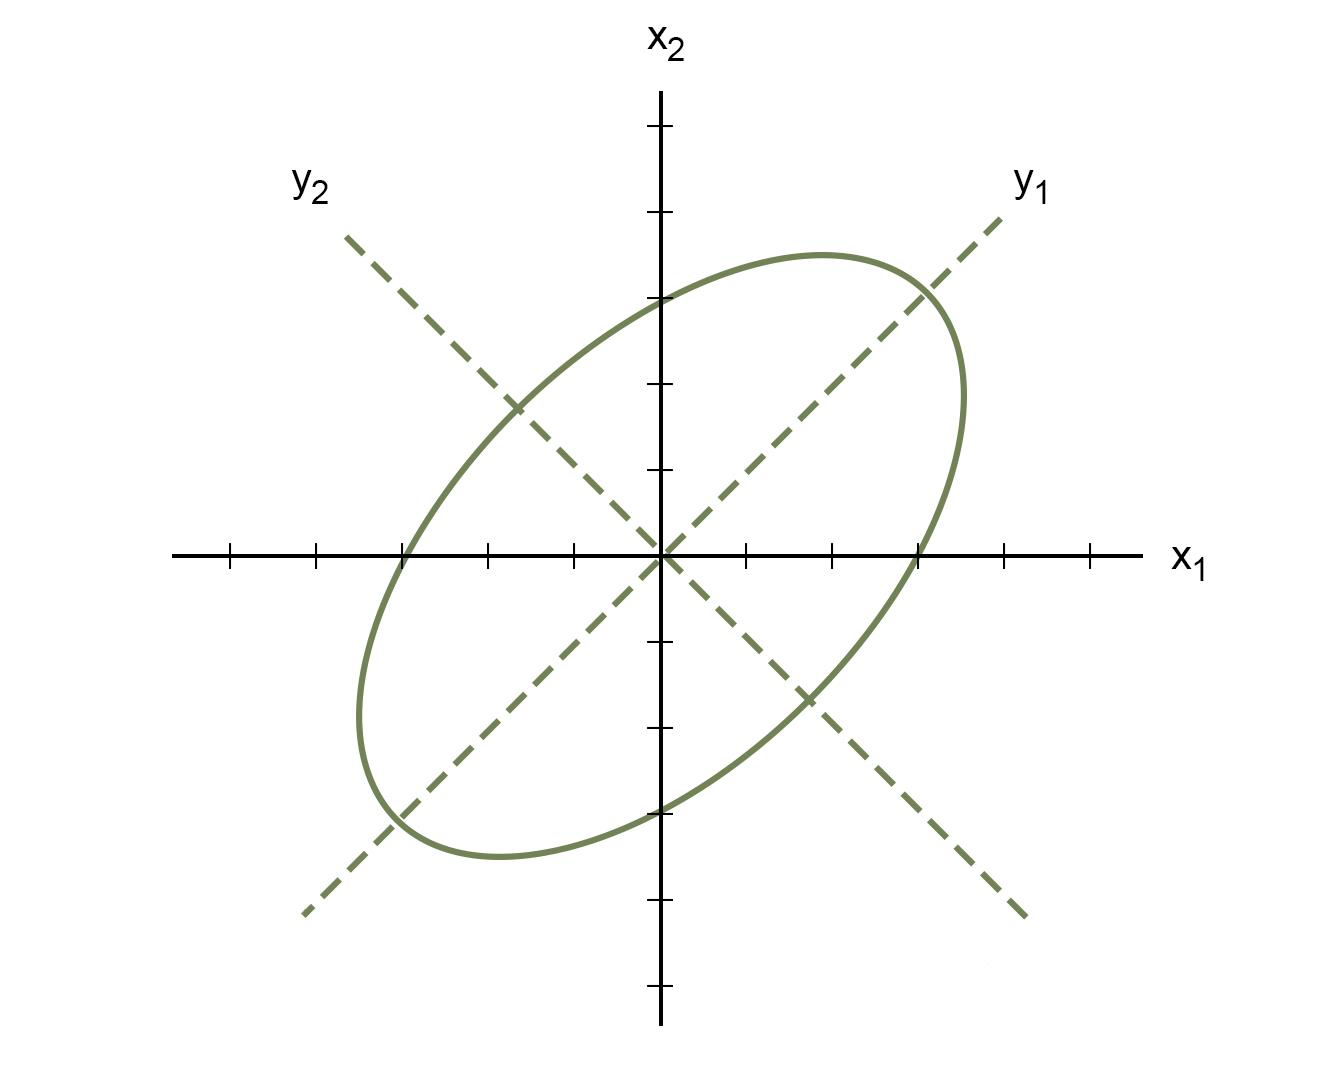
\includegraphics[width=0.75\textwidth]{Pictures/fig.29.jpg}
    \caption{Elipse}
    \label{Elipse}
\end{figure} 

  \bigskip
  
 El análisis anterior se resume en el Teorema siguiente:
 
 \bigskip
 
 \begin{corollary}\textbf{Teorema de los ejes principales para $\mathbb{R}^2$}.\index{Ejes principales $\mathbb{R}^2$}.
 
 Sea 
 \begin{equation}
a_{11}x_1^{2}+a_{12}x_1x_2+a_{22}x_2^{2}+ a_1 x_1 + a_2 x_2 + a = 0, 
\end{equation}
\noindent
la ecuación de una cónica $C$, y supongamos que 
 
 $$\bf{x} ^T A \bf{x}=a_{11}x_1^{2}+a_{12}x_1x_2+a_{22}x_2^{2}$$
 es la forma cuadrática asociada. Entonces, es posible  girar los ejes de coordenadas de modo que la ecuación para $C$ en el nuevo sistema de coordenadas $x^{\prime}y^{\prime}$ tenga la forma  
 
 $$\lambda_1x^{\prime 2}_1+\lambda_2x^{\prime 2}_2  +a_1^{\prime}x^{\prime}+ a_2^{\prime}y^{\prime} +a  =0$$
 \noindent
 donde $\lambda_1$   y  $\lambda_2$  son los autovalores de $A$. Se puede llevar a cabo la rotación por medio de la sustitución $\bold x=O \bold x^{\prime}$, donde $O$ diagonaliza a $A$ y $Det(O)=1$.
 \end{corollary}

 


\begin{figure}
    \centering
    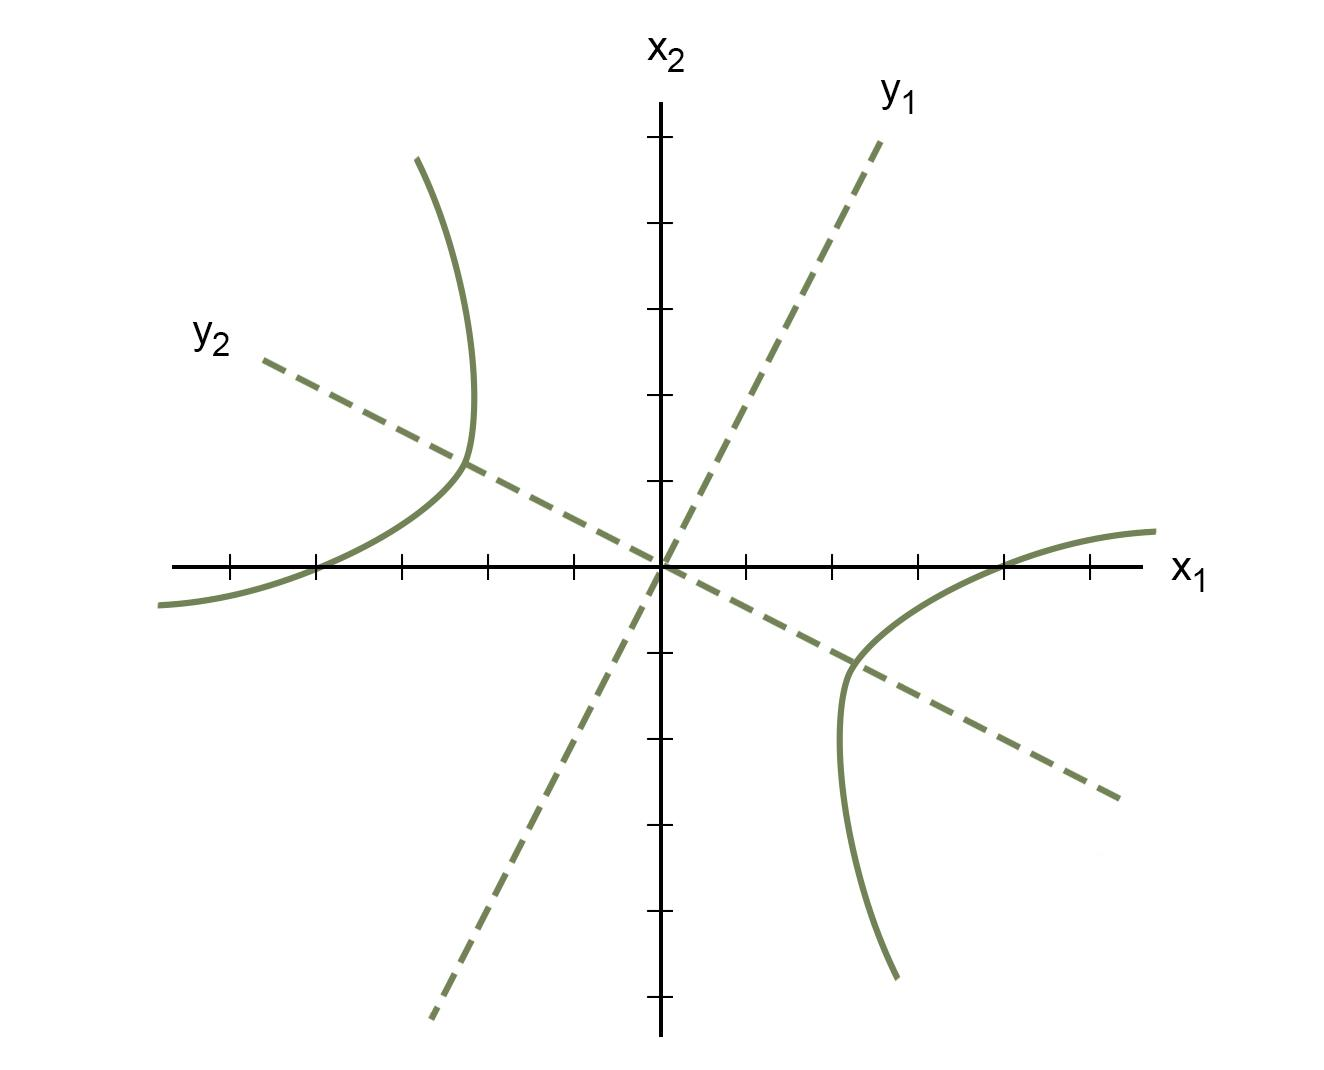
\includegraphics[width=0.75\textwidth]{Pictures/fig.30.jpg}
    \caption{Hipérbola}
    \label{Hipérbola}
\end{figure} 

Si $A$ es una matriz no diagonal, la gráfica   está girada hasta salirse de la posición estándar, como en las Figuras  \ref{Elipse} y \ref{Hipérbola}.
Encontrar los ejes principales (determinados por los vectores propios de $A$) equivale a
encontrar un nuevo sistema de coordenadas con respecto al cual la gráfica está en posición
estándar.

\bigskip

\subsection{Formas cuadráticas: aplicación a las superficies cuádricas}\index{Superficies cuádricas}
Sea
\begin{equation}
a_{11}x_1^{2}+a_{12}x_1 x_2+a_{13}x_1 x_3+a_{22}x_2^{2}+a_{23}x_2 x_3+a_{33}x_3^{2}+ a_1 x_1 + a_2 x_2+ a_3 x_3  + a = 0 \label{fcuadratica33}
\end{equation}
donde $a_{ij}$, $a_i$ ($i,j=1,3$) y $a$ son números reales  y al menos uno de los números $a_{ij}$ no es cero.
La parte principal

$$a_{11}x_1^{2}+a_{12}x_1x_2+a_{13}x_1x_3+a_{22}x_2^{2}+a_{23}x_2x_3+a_{33}x_3^{2}$$

\bigskip

 es la forma cuadrática asociada.

 \bigskip

 \bigskip
 
La Ec.(\ref{fcuadratica33}) puede escribirse en forma matricial

 \bigskip
 
\begin{equation*}
\left(\begin{array}{ccc} x & y & z 
\end{array}
 \right) \left(\begin{array}{ccc} a_{11} & a_{12}/2  & a_{13}/2  \\a_{12}/2 & a_{22} & a_{23}/2 \\a_{13}/2  & a_{23}/2 & a_{33}
\end{array}
 \right)  \left(\begin{array}{c} x \\y  \\z
\end{array}
 \right)+ \left(\begin{array}{ccc}a_1 & a_2& a_3
\end{array}
 \right) \left(\begin{array}{c} x \\y \\z 
\end{array}
 \right) +a=0\label{fcuadraticatodaR3
 }
\end{equation*}

 \bigskip
\begin{figure}
    \centering
    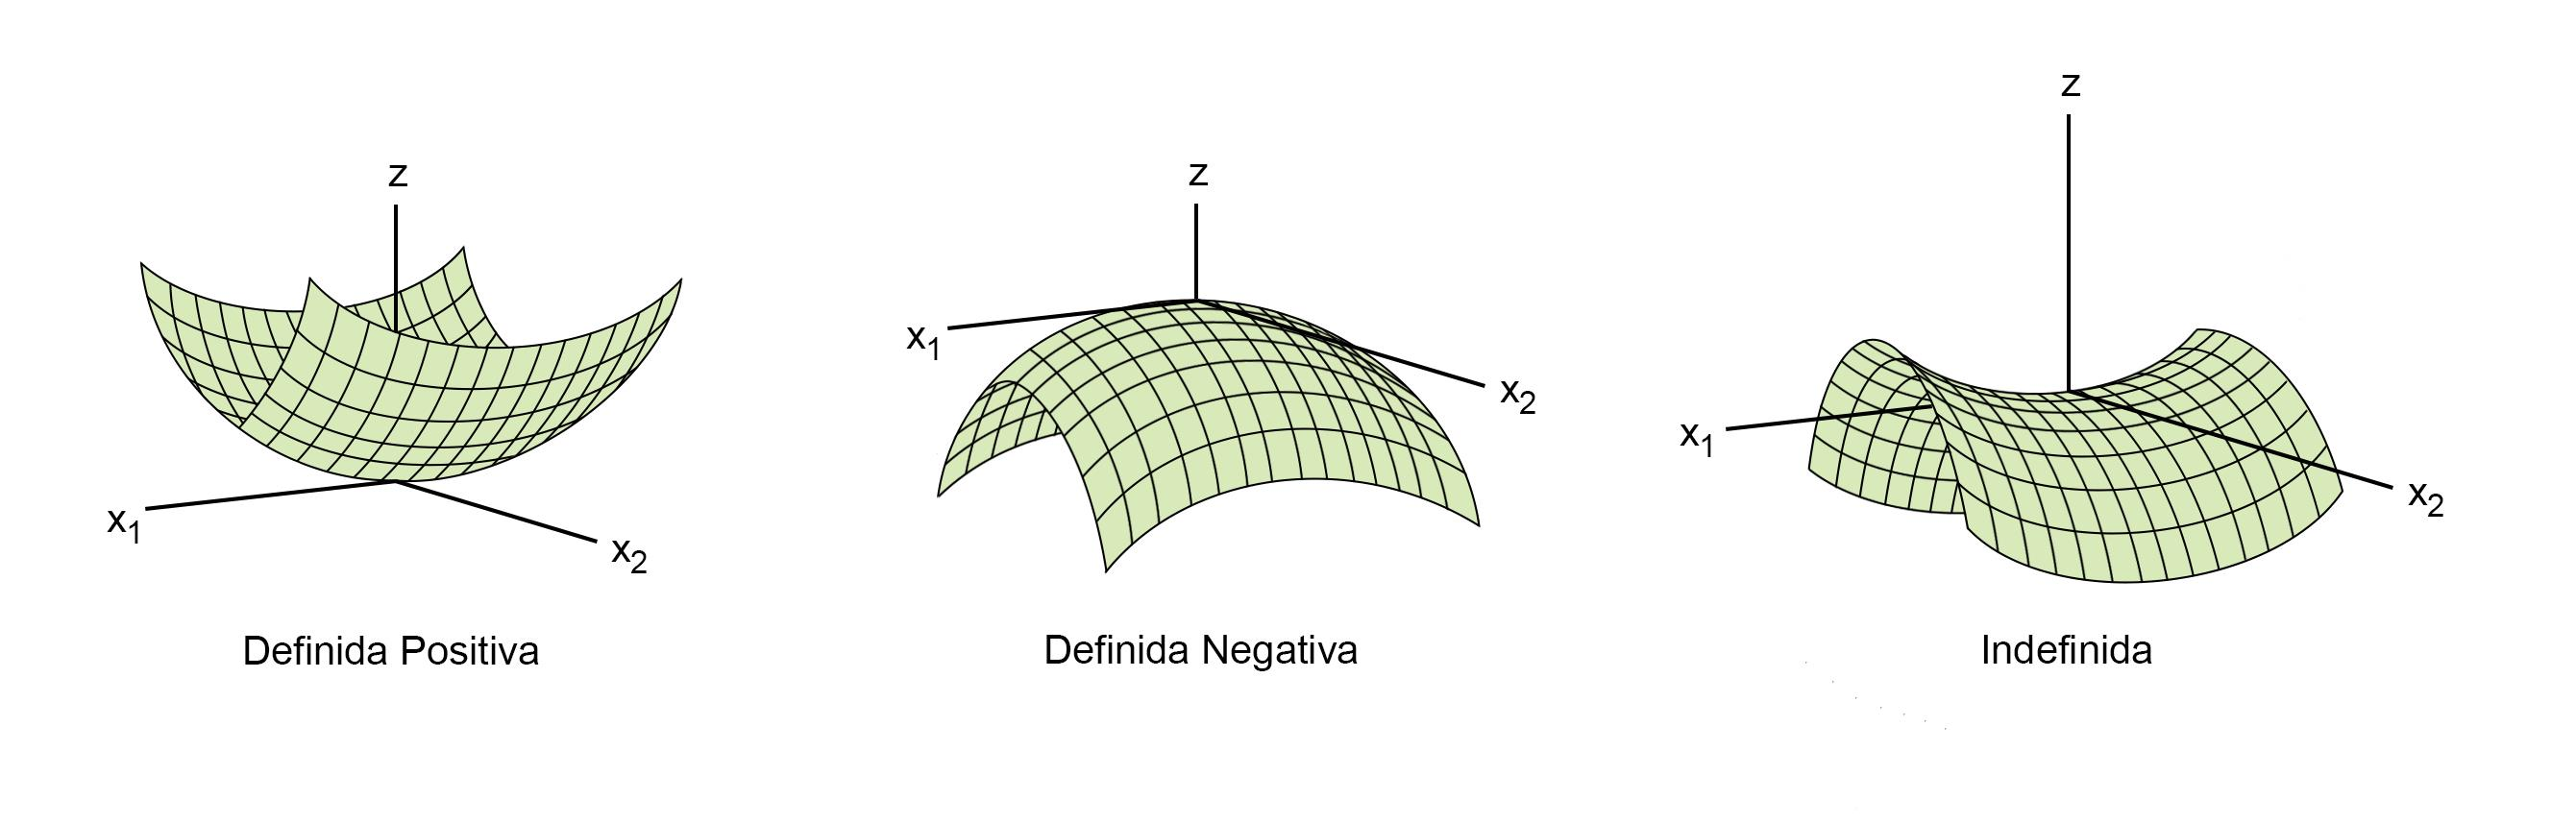
\includegraphics[width=1.1\textwidth]{Pictures/fig.31.jpg}
    \caption{Formas cuadráticas. a) Definida Positiva. b) Definida Negativa. c) Indefinida.}
    \label{FCUADRATICAS}
\end{figure} 

Se tiene el Teorema siguiente:

 \bigskip
 \begin{corollary}
     
 \textbf{Teorema de los ejes principales para $\mathbb{R}^3$}.
 
 Sea 
 \begin{equation*}
a_{11}x_1^{2}+a_{12}x_1x_2+a_{13}x_1x_3+a_{22}x_2^{2}+ 

a_{23}x_2x_3+a_{33}x_3^{2}+ a_1 x_1 + a_2 x_2+ a_3 x_3  + a = 0\label{fcuadratica3}
\end{equation*}


la ecuación de una cónica $C$, y supongamos que 
 
 $$\bf{x} ^T A \bf{x}=a_{11}x_1^{2}+a_{12}x_1x_2+a_{13}x_1x_3+a_{22}x_2^{2}+a_{23}x_2x_3+a_{33}x_3^{2}$$
 es la forma cuadrática asociada. Entonces se puede hacer girar los ejes de coordenadas de modo que la ecuación para $C$ en el nuevo sistema de coordenadas $x_1'x_2'x_3'$ tenga la forma  
 
 $$\lambda_1x^{\prime 2}_1+\lambda_2x^{\prime} 2_2+\lambda_3x^{\prime 2}_3  +a_1^{\prime}x_1^{\prime}+ a_2^{\prime}x_2^{\prime}+a_3 x_3^{\prime} +a  =0$$
 donde $\lambda_1$,   $\lambda_2$ y $\lambda_3$ son los autovalores de $A$. Como en el caso de $\mathbb{R}^2$ se puede llevar a cabo la rotación por medio de la sustitución $\bold x=O \bold x'$, donde $O$ diagonaliza a $A$ y $Det(O)=1$.
 \end{corollary}
 
 Este teorema sugiere el procedimiento para eleminar los términos de productos cruzados de una ecuación cuadrática en  $x_1$, $x_2$ y $x_3$. Y lo veremos con un ejemplo.
 
 \bigskip
 \begin{example}
 
 
 Se desea describir la superficie cuádrica cuya ecuación es 
 
 \begin{equation}
4x_1^{2}+4x_1x_2+4x_1x_3+4x_2^{2}+4x_2x_3+4x_3^{2}-3 = 0 \label{ejemplocuadrica}
\end{equation}

La forma matricial de la ecuación cuadrática anterior es 

\begin{equation}
\bf x ^T A \bf x -3 =0 \label{fcuadraticamatricialejemplo}
\end{equation}
  donde 
   
 \begin{equation}
  A=\left(\begin{array}{ccc} 4 & 2  & 2  \\2 & 4 & 2 \\2  & 2 & 4
\end{array}
 \right)
  \end{equation}
  
  Los autovalores de $A$ son $\lambda_1=\lambda_2=2$ y $\lambda_3=8$, y $A$ es diagonalizada ortogonalmente por la matriz  
  
  \begin{equation}
  O=\left(\begin{array}{ccc} -1/\sqrt 2  & -1/\sqrt 6   & 1/\sqrt 3   \\1/\sqrt 2  & -1/\sqrt 6  & 1/\sqrt 3  \\0  & 2/\sqrt 6 & 1/\sqrt 3
\end{array}
 \right)
  \end{equation}
 donde las dos primeras columnas de $O$ son los autovectores correspondientes a 
  $\lambda_1=\lambda_2=2$  mientras que la tercer  columna es un autovector correspondiente a 
$\lambda_3=8$. Se puede verificar que $Det(O)=1$ por lo que la transformación de coordenadas
$\bold x=O \bold x'$ es una rotación.

Al sustituir en la Ec.(\ref{fcuadraticamatricialejemplo})  se obtiene

\begin{equation}
\bf x^T O D O^T \bf x - 3 =  \bf x' D \bf x' -3 =0 \label{fcuadraticamatricialejemploprima}
\end{equation}

Y como 

\begin{equation}
  D= O^tAO=\left(\begin{array}{ccc} 2 & 0  & 0  \\0 & 2 & 0 \\0  & 0 & 8
\end{array}
 \right)
  \end{equation}
\noindent  
se tiene
  
  \begin{equation}
\left(\begin{array}{ccc} x^\prime & y^\prime & z^\prime
\end{array}
 \right) \left(\begin{array}{ccc} 2 & 0 & 0  \\0 & 2 & 0 \\0  & 0 & 8
\end{array}
 \right)  \left(\begin{array}{c} x^\prime \\y^\prime  \\z^\prime
\end{array}
 \right) -3=0\label{fcuadraticatodaR3ej
 }
\end{equation}
\noindent
o bien 
  
\begin{equation}
2(x_1^\prime)^{2}+2(x_2^\prime)^{2}+8(x_3^\prime)^{2}-3 = 0 \label{ejemplocuadricau}
\end{equation}
\noindent
que puede reescribirse

\begin{equation}
\frac {(x_1^\prime)^{2}}{3/2}+\frac {(x_2^\prime)^{2}}{3/2}+\frac {(x_3^\prime)^{2}}{3/8} = 1 \label{ejemplocuadricauu}
\end{equation}

\bigskip

y es la ecuación de un elipsoide.
\end{example}


\begin{remark}
Las superficies cuádricas han sido representadas en varios edificios contemporáneos.
Algunos de ellos son: Puente Juscelino Kubitichek, Brasilia (Brasil), Centro Nacional de las artes escénicas, Pekin (China), 
L'Oceanografic, Valencia (España).
\end{remark}

\textbf{ Formas cuadráticas y valores propios}  

 
Cuando $A$ es una matriz  de $n \times n$, la forma cuadrática $\mathbf{Q}(\bf x) = \bf{x}^T$$ A$$ \bf{x}$ es una función de
valores reales con dominio $\mathbb{R}^n$. Se distinguen varias clases importantes de formas cuadráticas
por el tipo de valores que asumen para diversos $\bf x$.


En la Figura  \ref{FCUADRATICAS} se muestran las gráficas de tres formas cuadráticas. Para cada punto
$\bf{x}$ $ = (x_1, x_2)$ del dominio de una forma cuadrática $\mathbf{Q}$, se traza un punto $(x_1, x_2, z)$, donde
$z = \mathbf{Q}(\bf x)$. Observe que excepto en $\bf x= \bf 0$, todos los valores de $\mathbf{Q}(\bf x)$ son positivos en la Figura \ref{FCUADRATICAS}(a) y  negativos en la Figura \ref{FCUADRATICAS}(b). En la Figura \ref{FCUADRATICAS}(c), en cambio, toma valores positivos y negativos.
De acuerdo a los autovalores de $A$ se tiene lo siguiente:


Sea $A$ una matriz simétrica de $n \times n$. Entonces una forma cuadrática $\bf x ^T$$ A$$ \bf x$ es:

\begin{itemize}
    \item 

\textit{definida positiva} si, y sólo si, todos los valores propios de $A$ son positivos,

\item 
\textit{definida negativa} si, y sólo si, todos los valores propios de $A$son negativos, o

\item 
\textit{
indefinida} si, y sólo si, $A$ tiene valores propios tanto positivos como negativos
\end{itemize}
\begin{remark}
Una de las aplicaciones más conocidas es  el estudio de extremos relativos  de funciones de varias variables. En ese caso se calculan los autovalores de la matriz Hessiana en los puntos estacionarios. Corresponde a un mínimo local en caso de ser definida positiva, a un máximo local en caso de definida negativa y a un punto silla si es indefinida.
\end{remark}

\bigskip


\newpage


%\begin{figure}
%\label{figproyxy}
    %\centering
    %
\includegraphics[width=0.60\textwidth]{Pictures/bilineal.png}    
    %\label{TLfig14}
%\end{figure}




\section{Actividades propuestas}



\begin{answers}
Realice un cuadro conceptual donde explique las diferentes superficies cuádricas.
Indique cuáles de ellas tienen centro, cuáles no, cuáles son degeneradas, y que significa ese término.
Investigue además, que carácteristica de los paraboloides hace que los radiotelescopios\index{Radiotelescopios} usen esa forma para sus antenas.
Complemente con imágenes de antenas de algún radiotelescopio y sus caracteristicas físicas
Se propone la presentación  oral del trabajo  con el fin de contribuir al desarrollo de  habilidades y capacidades del estudiante (15 minutos máximo).

\end{answers}

\subsection{Ejercicios}

\bigskip

%\subsubsection{Formas bilineales y cuadráticas.}

 \bigskip

\begin{exercise}
\item
Encuentre la matriz asociada a la forma bilineal
$\mathbf{A}(\vec{x},\vec{y})= x_1y_1-x_1y_2 + 2x_2y_1 + 6x_2y_2 - 3x_1y_3 + x_3y_3$
y calculale su rango.
\end{exercise}
\begin{exercise}
\item
Convierta la forma bilineal del ejercicio anterior en una forma cuadrática reemplzando $(\vec{x}=\vec{y})$.
Calcule su nueva matriz asociada.
\end{exercise}
\begin{exercise}
\item
Siendo que la matriz asociada a una forma cuadrática es simétrica haga una lista de todas las propiedades de las matrices
simétricas.
\end{exercise}

\begin{figure}
%\label{figproyxy}
    \centering
    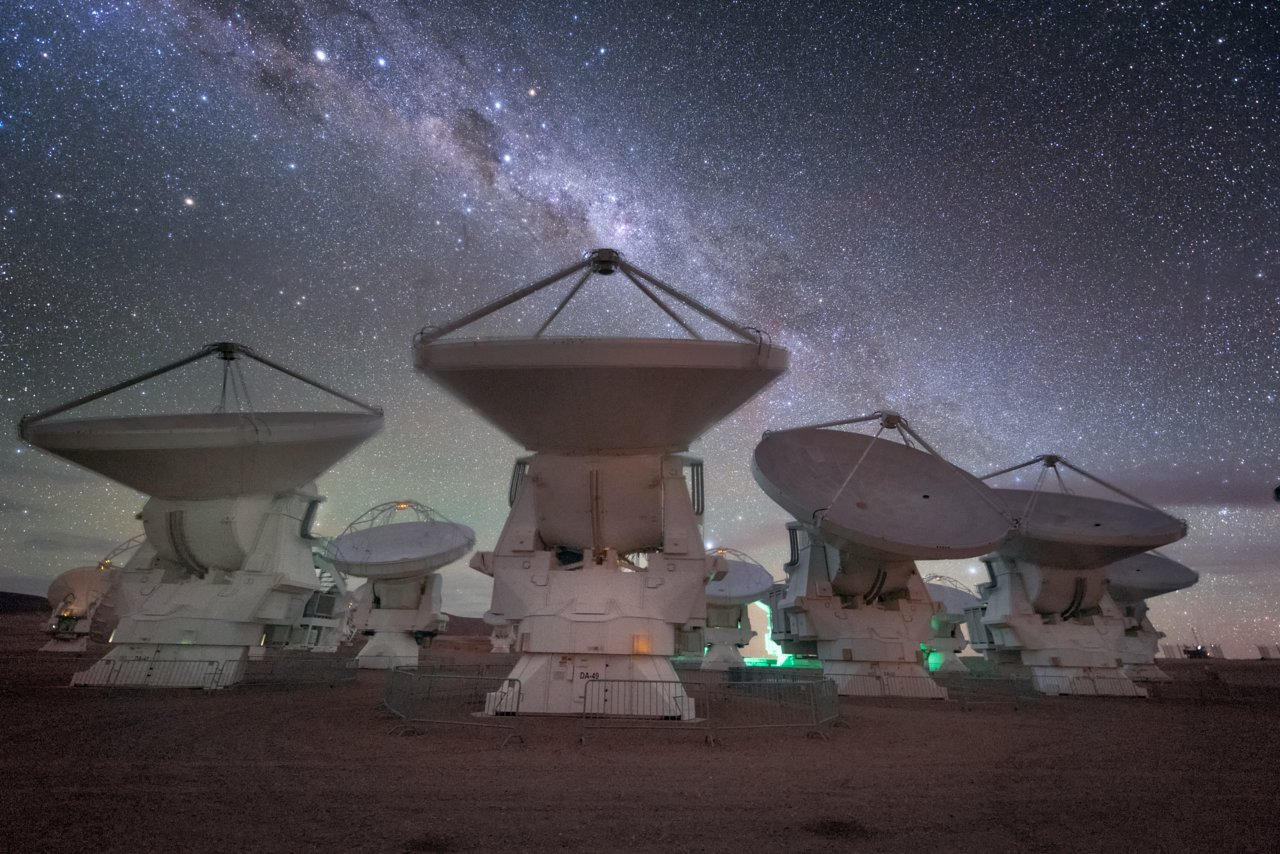
\includegraphics[width=0.70\textwidth]{Pictures/beletsky_alma_15-cc2.jpg}
\caption{Beletsky alma. https://www.eso.org/public/images/beletsky alma 15-cc2/}    
    \label{TELE}
\end{figure}

%\subsubsection{Forma canónica.}
\begin{exercise}
\item
Encuentre la forma canónica de la siguiente forma cuadrática:
$\mathbf{Q}(\vec{x})= x^2_2-3x^2_3 + 2x_1x_2 + x_1x_3$
\end{exercise}
\begin{exercise}
\item
Para la elipse $5x^2_1+5x^2_2 - 4x_1x_2 =48$, encuentre un cambio de variables por medio de calcular sus valores y vectores propios
unitarios tal que se elimine el producto cruzado de la ecuación.
\end{exercise}

\bigskip

%\subsubsection{Cónicas y su clasificación}

\vspace{0.25cm}
\begin{exercise}
\item
Especifique a que cónica corresponden las siguientes ecuaciones y especifique su centro.

\bigskip



a) $ (x-x_0)^2 + (y-y_0)^2=r^2$

b) $ (x-2)^2 - (y-3)^2=1$

c) $ x^2 +y^2 + 4x=1$
\end{exercise}

\newpage

\begin{exercise}
\item
Siendo la ecuación de una cónica:
$Ax^2+2Bxy+Cy^2+2Dx +2Ey+F=0$
Encuentre su forma matricial. Ayuda: Expresandola de la siguiente forma el elemento $a_{11}$ sería $F$, ¿cómo estarían relacionados los otros elementos de la matriz con la ecuación de la cónica?
  
  \begin{equation*}
\left(\begin{array}{ccc} 1 & x & y 
\end{array}
 \right) \left(\begin{array}{ccc} a_{11} &a_{12}  & a_{13}  \\a_{21} & a_{22} & a_{23} \\a_{31}  & a_{32} & a_{33}
\end{array}
 \right)  \left(\begin{array}{c} 1 \\x  \\y
\end{array}
 \right) =0\
\end{equation*}
Datos extras: Piense que las cónicas describen las órbitas. Ejemplo de órbitas elípticas pueden ser el  asteroide numerado 433 conocido con el nombre de Eros, en la página de  NEODyS (objetos cercanos al planeta Tierra) podrá encontrar muchos más.
Como ejemplo de órbita hiperbólica podría ser el  cometa C/2002 E2 Snyder-Murakami, y como ejemplo de órbita parábolica (excentricidad= 1) la del cometa C/2002 B2 LINEAR.

\bigskip

\end{exercise}
\begin{exercise}
\item
Usando la matriz del ejercicio anterior encuentre la forma de sus invariantes y especifique
de que tipo de cónica estamos hablando si $B^2-4AC=0$
\end{exercise}
\begin{exercise}
\item
Responda como estan los ejes de las cónicas con respecto a los ejes coordenados según:

a) $ B=0$

b) $ B\neq0$
\end{exercise}

\newpage

\begin{exercise}
\item
¿$\mathbf{Q}(\vec{x})= 3x^2_1+2x^2_2 + x^2_3 + 4x_1x_2 + 4x_2x_3$ es definida positiva?
\end{exercise}



 \subsection{ Autoevaluación}
 \label{Auto5}
 \bigskip



\subsubsection{Verdadero o Falso.}


 \bigskip
 
Dada una matriz simétrica:

\begin{enumerate}


 \item 
A es definida positiva si y solo si todos los valores propios de A son positivos.
\item
A es definida negativa si y solo si los valores propios van alternando entre positivos y negativos.
\item
A es indefinida si y solo si alguno de los valores propios es 0.
\item
Es posible clasificar A por medio de su determinante.
\item
Siempre exite un cambio ortogonal de la variable $\mathbf{x}=P\mathbf{y}$ tal que
$\mathbf{Q}(\mathbf{X})=\mathbf{x^t}A\mathbf{x}=\mathbf{y^t}D\mathbf{y}=\lambda_1x^2_1+\lambda_2x^2_2 + ... +\lambda_nx^2_n$
\end{enumerate}



\chapterimage{Pictures/blue_space(1).jpg}


\chapter{Cálculo tensorial}

Este capítulo trata de una introducción al estudio de tensores (escalar, vector, tensor de segundo orden y de orden superior). Se expone la notación indicial por su simplicidad  y facilidad de uso en las expresiones matemáticas. Se hace una revisión de las operaciones entre vectores, y de los sistemas de  coordenadas rectangulares. Luego se plantean los  sistemas de coordenadas curvilíneas, y la construcción de bases adecuadas. Para facilitar la comprensión  de los temas se presentan ejemplos y aplicaciones. El objetivo de incorporar el cálculo tensorial es  brindar al estudiante de Astronomía  herramientas matemáticas que le resulten de utilidad para los cursos superiores de la carrera.\\%\section{Tensores}

\section{ Invariancia y representación}





Dado un espacio vectorial, la elección de la base es arbitraria. Una vez elegida la base, lo que se tiene es una \textit{representación} del vector en una determinada base y por lo tanto, se tienen sus coordenadas.


Así para el vector $\mathbf{x}=(1,2,3)$, con las bases canónica, $B$ y la base $B^{\prime} =\left\{(1/2,0,0), (0,0,-2),(0,-1,0)\right\}$  se tendrán dos representaciones, 

$$\mathbf{x}= 1~\mathbf{e}_1+2~\mathbf{e}_2 +3~\mathbf{e}_3 $$

y 

$$\mathbf{x}= 2~\mathbf{e}^{\prime}_1+3/2~\mathbf{e}^{\prime}_2 -1~\mathbf{e}^{\prime}_3 $$.


En general, en un espacio vectorial de dimensión $N$, una vez elegida la base $B= \left\{\mathbf{e}_1,\mathbf{e}_2,\cdots, \mathbf{e}_n\right\}$, cada vector $\mathbf{x}$ estará representado por un conjunto de $n$ coordenadas representadas con $\lambda^j$
$$\sum_{j=1}^n~\lambda^j~\mathbf{e}_j$$
pero el  vector $\mathbf{x}$ es un \textit{invariante}, ya que  no depende de la base. De esta forma, dadas dos bases $B= \left\{\mathbf{e}_1,\mathbf{e}_2,\cdots, \mathbf{e}_n\right\}$  y $B ^{\prime}=\left\{\mathbf{e}^{\prime}_1,\mathbf{e}^{\prime}_2,\cdots, \mathbf{e}^{\prime}_n \right\}$  de un espacio vectorial $V$ de dimensión $n$, para un vector $\mathbf{x}$ se satisface la igualdad

$$\sum_{j=1}^n~\lambda^j~\mathbf{e}_j=\sum_{i=1}^n~\beta^i~\mathbf{e}^{\prime}_i$$
\begin{remark}
A diferencia de los capítulos anteriores, en este capítulo los vectores se indicarán en negritas.
\end{remark}


\section{Convenio de suma de Einstein}
\label{Convenio}
Albert Einstein, en 1916,  propuso un criterio que permite  escribir las sumas sin escribir los símbolos de sumatoria, dando origen a la notación indicial. Introdujo los dos convenios siguientes:  

\bigskip

\begin{enumerate}

\item Para un espacio vectorial de dimensión $N$, los índices  usados, ya sea como subíndices o como supraíndices pueden tomar todos los valores de $1$ a $N$, a no ser que se especifique lo contrario.

\item Si se repite un índice en un término, esto implica una suma con respecto a aquel índice desde $1$ a $N$. El índice repetido se llama índice \textit{mudo}.

\end{enumerate}

\bigskip

Usando los convenios anteriores, un vector  $\mathbf{x}$ puede  expresarse, entonces, 

\bigskip

$$\mathbf{x}=~\lambda^j~\mathbf{e}_j=~\beta^i~\mathbf{e}^{\prime}_i$$

\bigskip
En las expresiones anteriores $i$ y $j$ son índices mudos.

Así,


$$a_i^i~=~a_1^1~+~a_2^2~+~a_3^3~+\cdots~a_n^n~$$

\bigskip

Si los elementos $a_j^i$ son los de una matriz $ A \in \mathrm{R}^{n \times n}$,  (el supraíndice $i$ corresponde a la fila y el subíndice $j$ a la columna),  $a_i^i$ es la \textit{traza } de la matriz.
%, mientras  $a_{ii}$ es un elemento de la diagonal, uno sólo.
%(considerando que los índices que se repiten deben ser uno superior y otro inferior)

\bigskip


%\noindent
%Si la base $B$ es ortonormal  $ (\vec{e}_i.\vec{e}_j=\delta_{ij}~ \quad i,j=1,2,\cdots n)$, y si %$\vec{u}=~\beta^j~\vec{e}_j$

\bigskip

\begin{example}

En la expresión $$A_{ij}x_ix_j  \qquad  i,j=1,2,3$$ no hay índice libre, tanto $i$ como $j$ son índices mudos, por lo que al  sumar en $i$ y en $j$, el resultado da un escalar.
\end{example}

\bigskip 



\begin{remark}
Una de las ventajas de la notación indicial es que se tiene una expresión muy concisa. Así, un sistema  lineal de $3$ ecuaciones con $3$ incógnitas  usando el convenio de suma se escribe:
$$ a_{ij}x_j=b_i  \qquad  i,j=1,2,3.$$
%\hfill$\blacktriangle$
\end{remark}

\section{Notación indicial}




El sistema de coordenadas cartesianas rectangulares está definido por tres vectores, $\bold{i}$, $\bold{j}$, $\bold{k}$ que constituyen una base \textit{ortonormal}. Es decir que se satisfacen  dos propiedades:  son vectores  unitarios (longitud $1$) y  son ortogonales entre sí. El producto vectorial cumple la regla de la mano derecha: $ \bold{i} \times \bold{j}=\bold{k}  $, $ \bold{j} \times \bold{k}=\bold{i}  $ y $ \bold{k} \times \bold{i}=\bold{j}  $.

\bigskip

La representación de un vector $\bold{P}$ en un sistema de coordenadas rectangulares es:
\begin{equation}
\bold{P}= P_x \bold{i} + P_y \bold{j}  + P_z \bold{k}
\end{equation}
que puede reescribirse de la forma
\begin{equation}
\bold{P}= P_1 \bold{e}_1 + P_2 \bold{e}_2 + P_3 \bold{e}_3
\label{veccart}
\end{equation}
donde hemos considerado que $P_1 \equiv P_x$, $P_2 \equiv P_y$, $P_3 \equiv P_z$, $\bold{e}_1 \equiv \bold{i}$, $\bold{e}_2 \equiv \bold{j }$, $\bold{e}_3 \equiv \bold{k}$, como se indica en la Figura \ref{Tens_fig10}.

\begin{figure}[ht]
\begin{center}
\includegraphics[scale=0.4]{Pictures/Tens_fig10.jpg}
\caption{Vector en el sistema de coordenadas cartesianas.}
\label{Tens_fig10}
\end{center}
\end{figure}



La representación del vector  $\bold{P}$ de la  Ec.(\ref{veccart}) se expresa   con la notación indicial de la forma siguiente  (\cite{chaves}):
\begin{equation}
\bold{P}= P_i \bold{e}_i  \qquad (i=1,2,3)
\end{equation}

%Utilizando notación indicial los ejes del sistema de coordenadas son designados por la letra $x$ con un índice, 
%Por eso $x^i$ no representa un único valor sino $N$ valores si $i=1,2, \cdots, N$.


\subsection{Delta de Kronecker}\index{Delta de Kronecker}
El símbolo \textit{delta de Kronecker}, está definido por

\begin{eqnarray}
\label{Krone}
\delta_{ij} = \left \{
\begin{array}{ll}
1  & \mbox{ si $i=j$}, \\
                     0 & \mbox{ si  $i \neq j$}.
                     \end{array}
                     \right
\end{eqnarray}
\noindent                  
y  coincide con el resultado de hacer el producto escalar entre los vectores de  la base ortonormal $\bold{e}_i$, es decir que $\bold{e}_i   \cdot \bold{e}_j= \delta_{ij}$. Exponiendo esto en forma explícita se tiene:

   \begin{equation}
   \bold{e}_i. \bold{e}_j=
  \left(\begin{array}{ccc} \bold{e}_1 \cdot \bold{e}_1  & \bold{e}_1 \cdot \bold{e}_2  & \bold{e}_1 \cdot \bold{e}_3   \\ \bold{e}_2 \cdot \bold{e}_1 & \bold{e}_2 \cdot \bold{e}_2  & \bold{e}_2 \cdot \bold{e}_3  \\\bold{e}_3 \cdot \bold{e}_1   & \bold{e}_3 \cdot \bold{e}_2 & \bold{e}_3 \cdot \bold{e}_3
\end{array}
 \right) =    \left(\begin{array}{ccc} 1 & 0 & 0 \\0 & 1 & 0  \\0 & 0 & 1
 
\end{array}  \right) = \delta_{ij}
 \label{tensordelta}
\end{equation}

\bigskip


Este símbolo $\delta_{ij}$ es llamado \textit{operador de sustitución }, por la propiedad interesante que mostramos con un ejemplo.

Sea $\mathbf{v}$ un vector de componentes $v_i$, entonces

$$ \delta_{ij}v_i= \delta_{1j}v_1  +  \delta_{2j}v_2  +  \delta_{3j}v_3, $$
\noindent
como $j$ es un índice libre, se tiene:
\bigskip

Si $j=1$, $\delta_{i1}v_i= \delta_{11}v_1  +  \delta_{21}v_2  +  \delta_{31}v_3 =v_1 $

Si $j=2$, $\delta_{i2}v_i= \delta_{12}v_1  +  \delta_{22}v_2  +  \delta_{32}v_3 =v_2 $


Si $j=3$, $\delta_{i3}v_i= \delta_{11}v_1  +  \delta_{21}v_2  +  \delta_{31}v_3 =v_3 $

\noindent
de donde 
$$  \delta_{ij}v_i= v_j$$
\noindent
es decir, por la presencia de $\delta_{ij}$ se reemplaza en la componente $v_i$, el índice $i$ por el $j$. De ahí el nombre de operador de sustitución.

\subsection{Símbolo de Levi-Civita}\index{Símbolo de Levi-Civita}


El símbolo de permutación es llamado también de \textit{Levi-Civita} y está definido por:




\begin{equation}
\label{Levi}
 e_{i_1 i_2  \cdots i_N}=e^{i_1 i_2  \cdots i_N}=
\left\{ \begin{array} {lll} 
                    1 & \mbox{si los índices son distintos y son una permutación par}
\\
                    -1 & \mbox{si los índices son distintos y son una permutación  impar}\\
										 0 & \mbox{en otro caso} \\
                    
                   \end{array}
           \right.
\end{equation}

Es decir depende si  ${i_1 i_2 \cdots i_N}$   es una permutación par o impar de $1, 2, 3, \cdots,  N$.


Este símbolo es utilizado en la definición de determinante de una matriz de $N \times N$:


$$\left  | A \right  | = \sum_{i_1 i_2  \cdots i_N} e_{i_1 i_2  \cdots i_N} \quad a_{1i_1} a_{2i_2}  \cdots a_{Ni_N}$$

El determinante de una matriz $N \times N$ consiste en la suma de todos los productos posibles de $N$ elementos que pertenecen a distintas filas y columnas  multiplicados por $1$ o $-1$ de acuedo a si la permutación de los segundos índices es par o impar
.


\bigskip

En el caso $N=3$ se tiene lo siguiente:

$$e_{ijk}=e^{ijk}= \left[  ~\bold{e}_i~\bold{e}_j~\bold{e}_k   \right] $$



\begin{equation}
\label{Levi}
 e_{ijk}=e^{ijk}=
\left\{ \begin{array} {lll} 
                    1 & \mbox{si $ijk$ es una permutación par de $123$}
\\
                    -1 & \mbox{si $ijk$ es una permutación impar de $123$}\\
										 0 & \mbox{en otro caso} \\
                    
                   \end{array}
           \right.
\end{equation}

\bigskip

Y al calcular el determinante utilizando la definición anterior, se tiene la suma de seis términos, que son  todos los posibles productos de a tres elementos de la matriz

\[
\left  | \begin{array}{ccc}
a_{11}  & a_{12}   & a_{13}  \\
a_{21}  &  a_{22}   &  a_{23}  \\
a_{31}  &  a_{32}   &  a_{33}  
\end{array}
\right|=
\]

\bigskip

$$
=e_{123}~a_{11}a_{22}a_{33}+ e_{231}~a_{12}a_{23}a_{31}+e_{312}~a_{13}a_{21}a_{32}+

+e_{321}~a_{13}a_{22}a_{31}+e_{132}~a_{11}a_{23}a_{32}+e_{213}~a_{12}a_{21}a_{33}
$$


\bigskip

Luego, reemplazando los símbolos de permutación $e_{ijk}$ de acuerdo a (\ref{Levi}), resulta 
\[
\left  | A \right  |= 
a_{11}a_{22}a_{33}+ a_{12}a_{23}a_{31}+a_{13}a_{21}a_{32}-a_{13}a_{22}a_{31}-a_{11}a_{23}a_{32}-a_{12}a_{21}a_{33}
\]


\bigskip

Por otro lado, si se expresa el símbolo de permutación en función de la delta de Kronecker (u operador de sustitución), obtenemos

\begin{equation}
e_{ijk}=e_{lmn}~\delta_{li}\delta_{mj}\delta_{nk}
\end{equation}

\bigskip

\noindent
que es igual al resultado del determinante 


\[
e_{ijk}=\left  | \begin{array}{ccc}
\delta_{1i}  &\delta_{1j}   & \delta_{1k}  \\
\delta_{2i}  &  \delta_{2j}   &  \delta_{2k}  \\
\delta_{3i}  &  \delta_{3j}   &  \delta_{3k}  
\end{array}
\right|
\]


\begin{example}
 \[
e_{321}=\left  | \begin{array}{ccc}
\delta_{13}  &\delta_{12}   & \delta_{11}  \\
\delta_{23}  &  \delta_{22}   &  \delta_{21}  \\
\delta_{33}  &  \delta_{32}   &  \delta_{31}  
\end{array}
\right|= \left  | \begin{array}{ccc}
0  & 0   & 1  \\
0  &  1   &  0  \\
1  & 0   &  0  
\end{array}
\right|= -1
\]   
\end{example}

\section{Operaciones con vectores}
\noindent
\textbf{Producto escalar}\index{Producto escalar}

Dados 
$\bold{u}=~\beta^i~\bold{e}_i$ y  $\bold{v}=~\lambda^j~\bold{e}_j$ con $i,j=1,2, \cdots  n$
el producto escalar es 

\bigskip


$$\bold{u}.\bold{v}=~\beta^1 \lambda^1+ \beta^2 \lambda^2+ \cdots\beta^n\lambda^n = \beta^l\lambda^l $$



\bigskip

%Si suponemos que $\vec{e}^j=\vec{e}_j,j=1,2,\cdots n $, $\vec{v}=~\lambda^j~\vec{e}_j= ~\lambda_j~\vec{e}^j$, podemos  %reescribir el producto escalar $\vec{u}.\vec{v}$ de la forma siguiente:

\bigskip
Esto se obtiene al reemplazar  los vectores  $\vec{u}$ y $\vec{v}$, 
\begin{equation}
\bold{u}.\bold{v}= (~\beta^i~\bold{e}_i).~(\lambda^j~\bold{e}_j)=(~\beta^i \lambda^j) ~(\bold{e}_i.\bold{e}_j)
\label{producto escalar1}
\end{equation}

\bigskip
Usando (\ref{Krone}), como   $\bold{e}_i.\bold{e}_j=\delta_{ij}$, la ecuación ( \ref{producto escalar1}) queda
\begin{equation}
\bold{u}.\bold{v}= (~\beta^i \lambda^j) \delta_{ij}=  ~\beta^i\lambda^i
\label{producto escalar2}
\end{equation}
\bigskip

La  longitud de $\bold{u}$ puede escribirse

\bigskip


$$\left\|\bold{u}\right\|=\sqrt{\beta^i~\beta^i~}$$


La multiplicación de dos matrices $A\in \mathrm{R}^{m\times k }$ y $B\in \mathrm{R}^{k\times n }$ da por resultado una matriz $C\in \mathrm{R}^{m\times n }$. Si indicamos con el supraíndice la fila y con subíndice la columna,  los  elementos de la matriz $C$ son 

\bigskip


$$c^i_j=\sum_{l=1} ^k~a_l^i~b_j^l$$

\bigskip

\noindent
que se simplifica usando el convenio de Einstein a 

$$c^i_j=~a_l^i~b_j^l.$$

\bigskip

\noindent

\begin{remark}
Note que $c^i_j$ tiene dos índices libres. No es un escalar, porque no están todos los índices afectados a sumatorias.
%\hfill$\blacktriangle$
\end{remark}
\newpage
\noindent
\textbf{Producto vectorial}\index{Producto vectorial}

Si $\bold{u_i}= ~\beta_i^j~\bold{e}_j$  son vectores de $\mathrm{R}^{3}$, $i=1,3$, el producto vectorial  de $\bold{u_1}$ y $\bold{u_2}$ da como resultado un vector:
\begin{equation}
\bold{u}_1 \times\bold{u}_2= e_{ijk}~\beta_1^j~\beta_2^k~~\bold{e}_i
\label{producto vectorial}
\end{equation}
donde $e_{ijk}$ es el símbolo de permutación. 
\bigskip
Esa expresión se obtiene a partir de calcular el determinante 

\[
\bold{u}_1 \times\bold{u}_2=\left  | \begin{array}{ccc}
\bold{e}_1  & \bold{e}_2  & \bold{e}_3 \\
\beta_1^1 &  \beta_1^2  &  \beta_1^3 \\
\beta_2^1 &  \beta_2^2  &  \beta_2^3 
\end{array}
\right|=c_1 \bold{e}_1 + c_2 \bold{e}_2  + c_3 \bold{e}_3,
\]

\bigskip
\noindent
donde 
\[
c_1 = \beta_1^2 \beta_2^3 - \beta_2^2  \beta_1^3 \\
c_2 = - \beta_1^1  \beta_2^3  +  \beta_2^1   \beta_1^3  \\
c_3= \beta_1^1  \beta_2^2  - \beta_2^1  \beta_1^2  
\]

Teniendo en cuenta la definición de los símbolos de permutación (\ref{Levi}),  pueden reescribirse 
\[
c_1=e_{123} \beta_1^2 \beta_2^3  + e_{132} \beta_2^2 \beta_1^3 \\
c_2 = e_{231} \beta_1^1  \beta_2^3  + e_{213} \beta_2^1   \beta_1^3  \\
c_3=   e_{312} \beta_1^1  \beta_2^2 +  e_{321} \beta_2^1  \beta_1^2  
\]
luego, en forma reducida, usando la notación de Einstein,


$$c_i=e_{ijk} \beta_1^j \beta_2^k$$  

\noindent
y de ahí se obtiene la expresión (\ref{producto vectorial}).






\bigskip

\begin{example}


Si se desarrolla la expresión $c_i=e_{ijk} A^j B^k $ para $i=1$, se tiene:

\bigskip

\begin{eqnarray*}
c_1&=&e_{1jk} A^j B^k \\
c_1&=& e_{11k} A^1 B^k + e_{12k} A^2 B^k + e_{13k} A^3 B^k \\
c_1&=& e_{111} A^1 B^1 + e_{112} A^1 B^2 + e_{113} A^1 B^3 +  e_{121} A^2 B^1 + e_{122} A^2 B^2 +\\
 &&  + ~ e_{123} A^2 B^3 +    e_{131} A^3 B^1  + e_{132} A^3 B^2  + e_{133} A^3 B^3
\end{eqnarray*}


\bigskip

De acuerdo a la definición de los símbolos de permutación (\ref{Levi}) son nulos los términos con índices repetidos, entonces resulta


\begin{eqnarray*}
c_1=e_{123} A^2 B^3 + e_{132} A^3 B^2= A^2 B^3 - A^3 B^2 
\end{eqnarray*}
\end{example}


\noindent
\textbf{Producto mixto}\index{Producto mixto}

Si $\bold{u}_l=\beta_l^i~\bold{e}_i$  y anotamos como $\left[\bold{u}_1\bold{u}_2\bold{u}_3\right]$ al producto mixto,

 $$\left[\bold{u}_1\bold{u}_2\bold{u}_3\right]= \bold{u}_1.(\bold{u}_2\times\bold{u}_3)$$

\noindent
se tiene que 

\bigskip

$$\left[\bold{u}_1\bold{u}_2\bold{u}_3\right]=\left[ ~\beta_1^i~\bold{e}_i  ~\beta_2^j~\bold{e}_j ~\beta_3^k~\bold{e}_k \right]$$

\bigskip


$$=~\beta_1^i~\beta_2^j~\beta_3^k\left[  ~\bold{e}_i~\bold{e}_j~\bold{e}_k   \right]$$

\bigskip

$$=~\beta_1^i~\beta_2^j~\beta_3^k ~e_{ijk}$$


\bigskip


\noindent
o sea, es el determinante de la matriz de las coordenadas $\beta_j^i $, 

\bigskip

$$\left[\bold{u}_1\bold{u}_2\bold{u}_3\right]=\left|\beta_j^i  \right|$$



\bigskip

\noindent
\textbf{Producto tensorial}\index{Producto tensorial}

El producto tensorial o diádico entre dos vectores $\bold{u}$  y $\bold{v}$ está definido de la forma siguiente:

\begin{equation}
\bold{u} \otimes \bold{v}=  \left[ \begin{array}{c} u_1 \\ u_2
\\  u_3
\end{array}
 \right]  \otimes   \left[ \begin{array}{c} v_1 \\ v_2
\\  v_3
\end{array}
 \right] = \left[ \begin{array}{ccc} u_1 v_1  & u_1 v_2 & u_1 v_3 \\ u_2 v_1  & u_2 v_2 & u_2 v_3
\\  u_3 v_1  & u_3 v_2 & u_3 v_3
\end{array}
 \right]
 \label{ptensvectores}
\end{equation}

\bigskip


Se obtiene una matriz $\bold{A}$, $\bold{A}= \bold{u} \otimes \bold{v} $, donde, por ejemplo, $ u_3 v_2 $ es la  componente de la fila  $3$, y columna $2$. En este caso particular, el producto tensorial es el producto   matricial usual  de los vectores $ \bold{u}$ (de $n \times 1$)  y  $\bold{v}^t$, (de $1 \times n$). 


Una matriz $\bold{A}$ puede escribirse en términos de los productos tensoriales de los vectores de la base $~\bold{e}_1$, $~\bold{e}_2$, y $~\bold{e}_3  $, de la forma siguiente:

\bigskip

\begin{equation}
\bold{A}= \bold{u} \otimes \bold{v}=
u_1 v_1 \left( \begin{array}{ccc} 1  & 0   & 0 \\ 0    & 0 & 0
\\  0 & 0 & 0
\end{array}
 \right)+  u_1 v_2 \left( \begin{array}{ccc} 0  & 1   & 0 \\ 0    & 0 & 0
\\  0 & 0 & 0
\end{array}
 \right)+ 
 
+ u_1 v_3 \left( \begin{array}{ccc} 0  & 0   & 1 \\ 0    & 0 & 0
\\  0 & 0 & 0
\end{array}
 \right)+ \cdots u_3 v_3 \left( \begin{array}{ccc} 0  & 0   & 0 \\ 0    & 0 & 0
\\  0 & 0 & 1
\end{array}
 \right)
\end{equation}




\begin{equation}
\bold{A}= \bold{u} \otimes \bold{v}= u_1v_1 ~ \bold{e}_1 \otimes \bold{e}_1 + u_1v_2  ~\bold{e}_1 \otimes \bold{e}_2 +  \cdots  u_3v_3  ~\bold{e}_3 \otimes \bold{e}_3
\end{equation}

\bigskip

\noindent
que, utilizando el convenio de Einstein, puede  reescribirse
 

\begin{equation}
\bold{A}= \bold{u} \otimes \bold{v}= u_iv_j ~\bold{e}_i \otimes \bold{e}_j 
\end{equation}


\section{ Transformaciones lineales}


%%%%%OJO  ver apunte de tensores de Exactas

Sea $T: V \rightarrow W$ una transformación lineal entre dos espacios vectoriales $V$ y $W$ (ver Definición \ref{TL}).
Sean $B= \left\{\bold{v}_1,\bold{v}_2,\cdots, \bold{v}_N\right\}$ una base  de $V$ y $\bar{B}= \left\{\bold{w}_1,\bold{w}_2,\cdots, \bold{w}_m\right\}$ una base  de $W$. Si aplicamos $T$ a un vector arbitrario $\bold{v}\in V$, 



$$\bold{v}= ~\alpha^j~\bold{v}_j$$



$$T(\bold{v})= T(\alpha^j~\bold{v}_j)= ~\alpha^j~T(\bold{v}_j)$$

\bigskip

Como $T(\bold{v})$ es un elemento de $W$, se puede escribir como combinación lineal de los vectores de la base de $W$, 



$$T(\bold{v})= ~\beta^i~\bold{w}_i$$

\bigskip
Por otro lado, si se aplica $T$ a los vectores de la base de $V$, se obtiene la expresión 

 $$T(\bold{v}_j)=a_j^i~\bold{w}_i$$

\bigskip
\noindent
donde los escalares $a_i^j$ son las coordenadas $T(\bold{v}_j)$ en la base de $W$. 


En la expresión  anterior   el término $a_j^i$  tiene dos índices: $j$ está asociado al espacio  $V$ e $i$ al espacio $W$. $T$ es la matriz de la transformación lineal, en cada columna $j$ están las coordenadas de $T(\bold{v}_j)$ en la base de $W$.


$$T(\bold{v})=~\alpha^j~T(\bold{v}_j)= \alpha^j a_j^i~\bold{w}_i$$



$$T(\bold{v})= ~\beta^i~\bold{w}_i= a_j^i \alpha^j ~\bold{w}_i$$

\bigskip


\noindent
de donde,
 


$$ (~\beta^i~ - a_j^i \alpha^j ) ~\bold{w}_i=\bold{0}$$

\bigskip


\noindent
y por ser los $\bold{w}_i$ linealmente independientes (forman una base de $W$), resulta 



$$ \beta^i~ = a_j^i \alpha^j $$

\bigskip
\noindent
que da la relación entre las coordenadas  de $\bold{v}$ y de $T(\bold{v})$. Corresponde al producto matricial 




%$$A=\left(\begin{array}{cccc} a_{11} & a_{12}&  \cdots & a_{1n} \\a_{21}  & a_{22} & \cdots & a_{2n}
%\\  \cdots & \cdots  &  \cdots  & \cdots \\ a_{n1} & a_{n2} & \cdots & a_{nn}
%\end{array}
% \right)$$

%$$\left[ \begin{array}{c} \beta^1 \\ \beta^2 
%\\  \beta^3\\ \cdots \\ \beta^n
%\end{array}
% \right]  \left[\begin{array}{cccc} a_{1}^1 & a_{2}^1&  \cdots & a_{n}^1 \\a_{1}^2  & a_{2}^2 & \cdots & %a_{n}^2
%\\  \cdots & \cdots  &  \cdots  & \cdots \\ a_{1}^n & a_{2}^n & \cdots & a_{n}^n
%\end{array}
% \right]\left[\begin{array}{c} \alpha^1 \\ \alpha^2   
%\\  \alpha^3  \\ \cdots \\ \alpha^n  
%\end{array}\right] $$


\bigskip

\begin{equation}
    \left(\begin{array}{c} \beta^1 \\ \beta^2 
\\  \beta^3\\ \cdots \\ \beta^n 
\end{array}
 \right)=\left(\begin{array}{cccc} a_{1}^1 & a_{2}^1&  \cdots & a_{n}^1 \\a_{1}^2  & a_{2}^2 & \cdots & a_{n}^2
\\  \cdots & \cdots  &  \cdots  & \cdots \\ a_{1}^n & a_{2}^n & \cdots & a_{n}^n
\end{array}
 \right)\left(\begin{array}{c} \alpha^1 \\ \alpha^2   
\\  \alpha^3  \\ \cdots \\ \alpha^n  
\end{array}\right)
\end{equation}

\bigskip


En los elementos de la matriz el supraíndice $i$ y el subíndice $j$ del elemento $a_j^i$ corresponden a la fila y  a la columna  respectivamente. Es la matriz asociada a la transformación lineal $T$ definida en la Sección \ref{MatrizdeunaTL}).

\bigskip

\begin{example}
\label{ejuiyei}
\noindent
Si la transformación lineal  es la identidad, usamos dos bases distintas, $B=\left\{\bold{e}_1,\bold{e}_2\right\}$ y $B^\prime=\left\{\bold{u}_1,\bold{u}_2,\right\}$, y las coordenadas en cada base son  $\bold{v}= ~\beta^j~\bold{e}_j=~\alpha^j~\bold{u}_j$,   la relación entre las coordenadas es 
$$ \beta^i~ = a_j^i \alpha^j .$$


$$\left(\begin{array}{c} \beta^1 \\ \beta^2 
 \end{array}
 \right)= \left(\begin{array}{cc} a_{1}^1  &a_{2}^1  \\ a_{1}^2\ &  a_{2}^2
\end{array}
 \right)\left(\begin{array}{c} \alpha^1 \\ \alpha^2 
 \end{array}
 \right)$$
 
 \bigskip
 
Estas expresiones se  corresponden con las Ecs.(\ref{ec4}) y (\ref{XPAX}),  donde se vio la relación  entre  las coordenadas del vector $\vec{x}$ en la antigua base  $B$  y en la nueva base $B ^{\prime}$, respectivamente, $x^i$ y $x^{ \prime i}$, con $i=1,2$. En forma matricial, $X=AX^{\prime}$, o 



\begin{equation}
\left\{ \begin{array} {ccl} 
                    x^1&\ =&   a^1_{1}x^{\prime 1}+a^1_{2}x^{\prime 2}    \\
                     x^2 &\ = &a^2_{1}x^{\prime 1}+a^2_{2}x^{\prime 2} 
                   \end{array}
           \right.
\end{equation}



\bigskip

Si $\bold{u}_1=(2,3)$ y $\bold{u}_2=(1,4)$ 
usando lo anterior, para el vector  

\bigskip



$$\left(\begin{array}{c} 7 \\ 7
 \end{array}
 \right)_B=\left(\begin{array}{cc} 2  & 1 \\ 3  &  4
\end{array}
 \right)
\left(\begin{array}{c} 3 \\ 1
 \end{array}
 \right)_{B^\prime}= P_{B,B ^{\prime}}\left(\begin{array}{c} 3 \\ 1
 \end{array}
 \right)_{B^\prime}$$

\bigskip




\bigskip

La relación está dada por la matriz de cambio de base de $B^\prime$ a $B$, $P_{B,B ^{\prime}}$ vista en la  Sección \ref{Cambio de base}.


\bigskip


Por otro lado,  La relación entre los vectores de las bases  $B^\prime$  y $B$ está dada por la matriz transpuesta  (Ver Ec.(\ref{matriz Acb}) en la Sección (\ref{Cambio de base})):



\begin{equation*} \label{rot}
\left\{ \begin{array} {ccl} 
                    \bold{u _1} &\ =&   a_{1}^1\bold{e}_1+a_{1}^2\bold{e}_2 =2\bold{e}_1+3\bold{e}_2   \\
                     \bold{u _2 } &\ = &a_{2}^1\bold{e}_1+ a_{2}^2\bold{e}_2 =1\bold{e}_1+4\bold{e}_2  \\
										\end{array}
           \right.
\end{equation*}

\bigskip


Usando el convenio, la relación entre los vectores de las bases tiene la expresión


 $$ \bold{u}_j~ = a_j^l \bold{e}_l$$

\end{example}

%\subsection{Transformaciones de coordenadas ortogonales}


%\bigskip

\noindent
 %mientras que la  relación entre  las coordenadas de un mismo vector en las bases $B$ y $B^\prime$  (ver %Sección(\ref{RELCOORD}), Ec.(\ref{ec4})), está dada por:






\section{Definición de tensor}


El concepto de \emph{tensor} tiene su origen en la evolución de la geometría diferencial de Gauss, Riemann y Christoffel. La necesidad del cálculo tensorial, como rama sistemática de la matemática, se debe a Ricci y a su discípulo Levi-Civita, que publicaron en colaboración el primer trabajo sobre esta materia: \emph{Métodos del cálculo diferencial absoluto y sus aplicaciones}, en Mathematische Annalen, vol. 54 (1901).



El objeto principal del cálculo tensorial es la investigación de las relaciones que permanecen invariantes cuando se cambia de un sistema de coordenadas a otro. Las leyes de la física no pueden depender del sistema de referencia que elija el físico con fines descriptivos. Por eso es, estéticamente deseable y muchas veces conveniente, utilizar el cálculo tensorial como fundamento matemático en que se puedan formular tales leyes. Einstein, en particular, lo consideró un excelente instrumento para la presentación de su teoría general de la relatividad. El cálculo tensorial alcanzó gran importancia y es hoy en día inapreciable en sus aplicaciones en la mayoría de las ramas de la física teórica; es también indispensable en  geometría diferencial.




\begin{figure}[hbtp]
%\centering
\begin{center}
%\includegraphics[scale=0.35]{Pictures/VIDEO_tensores.png}
%\caption{}
\end{center}
\end{figure}

\bigskip


%Los tensores se definen en función de sus propiedades de transformación ante un cambio de coordenadas:
\subsection{Cambio de coordenadas}




Si se considera un espacio vectorial $V$ de dimensión $N$ con el sistema de coordenadas $  x^1, x^{2}, x^{3},\cdots,x^{n}$, las $N$ ecuaciones 




\begin{equation}
x^{\prime i} = x^{\prime i}( x^1, x^{2}, x^{3},\cdots,x^{n} )= \varphi ^i( x^1, x^{2}, x^{3},\cdots,x^{n} ), \qquad i=1, \cdots N
\label{cambiocoord}
\end{equation}

\bigskip
\noindent
donde $  \varphi ^i$  son funciones continuas y diferenciables de las coordenadas  definen un nuevo sistema de coordenadas  $  x^{\prime 1}, x^{\prime 2}, \cdots, x^{\prime N}$.

\bigskip

La condición necesaria y suficiente para que las Ec.(\ref{cambiocoord}) definan una transformación de coordenadas 
es que el Jacobiano formado por las derivadas parciales $  \frac{\partial  x^{\prime i}}{\partial   x^{j}}$ no se anule.
En ese caso se pueden resolver para las $  x^i$  como funciones de $  x^{\prime i}$ y se obtiene, 
\begin{equation}
x^{i} = \psi ^i( x^{\prime 1}, x^{\prime 2}, \cdots, x^{\prime N} ), \qquad i=1, \cdots N
\label{cambiocoord2}
\end{equation}


\bigskip

\begin{example}
\label{ejrelcont2}
 En el caso particular de un cambio de base en $\mathbb{R}^3$   la relación entre las coordenadas está dada por el sistema lineal (\ref{ec4}) para $n=3$


\begin{equation}
\left\{ \begin{array} {ccl} 
                    x^1&\ =&   a^1_{1}x^{\prime 1}+a^1_{2}x^{\prime 2}+a^1_{3}x^{\prime 3}    \\
                     x^2 &\ = &a^2_{1}x^{\prime 1}+a^2_{2}x^{\prime 2}+a^2_{3}x^{\prime 3} \\
                    x^3 &\ =&a^3_{1}x^{\prime 1}+a^3_{2}x^{\prime 2}+a^3_{3}x^{\prime 3}
                   \end{array}
           \right.
\end{equation}

Corresponde a  relaciones como  las de la Ec.(\ref{cambiocoord2}). El determinante de la matriz Jacobiana (cuyos elementos son $  \frac{\partial  x^{i}}{\partial   x^{\prime}_j}= a^i_{j}$) no se anula, porque   la matriz de cambio de base $A$ tiene inversa. Con su matriz inversa  pueden escribirse  las ecuaciones    (\ref{cambiocoord}) y así tener   las coordenadas $x^{\prime i}$ como funciones de las  $x^i$.
\end{example}
\subsection{Tensores de orden $0$, $1$ y $2$}
\label{T012}
Es importante tener presente la expresión  (\ref{XPAX})  de la relación ya vista  entre las coordenadas $x^{\prime i}$ y $x^{i}$  ante un cambio de base. Porque los tensores se definen en función de sus propiedades de transformación ante un cambio de coordenadas  (\cite{spain}).:
\begin{equation}
\label{Cambiocoord}
x^{i} \rightarrow x^{\prime i}  \qquad i=1,\cdots,N
\end{equation}
dado por las relaciones de las Ecs.(\ref{cambiocoord}) y (\ref{cambiocoord2}).

\bigskip

Se tiene lo siguiente:

\bigskip

\begin{itemize}
\item
\textbf{Tensor de orden cero o escalar} es una cantidad $\phi$ que permanece invariante al cambiar al sistema primado,

$$\phi^{\prime}=\phi$$

\textcolor{blue}{Ejemplos}
La masa, la energía, la temperatura.

\bigskip

 \item
\textbf{Tensor de orden uno o vector} son $N$ cantidades



\bigskip
\begin{itemize}
\item  
\textbf{Vectores contravariantes}

Las funciones $  v^{j}$   de las $N$ coordenadas $  x^{i}$  se dice que son las componentes de un \textit{vector contravariante} si se transforman según la ecuación:


\begin{equation}
v^{\prime i} = \sum^{n}_{i=1} \frac{\partial  x^{\prime i}}{\partial   x^{j}} \quad v^{j} = \frac{\partial  x^{\prime i}}{\partial   x^{j}} \quad  v^{j} \qquad i=1,\cdots,n 
\label{contravariante}
\end{equation}
en un cambio de coordenadas de $ x^{i}$  a $ x^{\prime i}$.
  
\bigskip

\textcolor{blue}{Ejemplo}  
Los diferenciales $d x^{\prime i} $,  
\[d x^{\prime i}= \frac{\partial  x^{\prime i}}{\partial   x^{j}} \quad  dx^{j}   \]
forman las componentes de un vector contravariante, ya que 
se transforman de la misma forma que la expresión (\ref{contravariante}).
\bigskip 

\item 

\textbf{Vectores covariantes}

Las funciones $  v_{j}$   de las $N$ coordenadas $  x^{i}$  se dice que son las componentes de un \textit{vector covariante} si se transforman según la ecuación:


\begin{equation}
v_i^{\prime}=\frac{\partial  x^{j}}{\partial   x^{\prime i}} \quad  v_{j}
\label{covariante}
\end{equation}
en un cambio de coordendas de $ x^{i}$  a $ x^{\prime i}$.
\bigskip
Ejemplo.
El vector gradiente de una función $f$
\begin{equation}
\frac{\partial  f }{\partial   x^{\prime i}}=\frac{\partial  f}{\partial   x^{j}} \frac{\partial  x^{j}}{\partial   x^{\prime i}}= \frac{\partial  x^{j}}{\partial   x^{\prime i}}\frac{\partial  f}{\partial   x^{j}}
\end{equation}
De acuerdo a la Ec.(\ref{covariante}) las magnitudes $  \frac{\partial  f}{\partial   x^{j}}$  son las componentes de un vector covariante (en esa expresión el índice $j$ es considerado un subíndice).



\bigskip 

\textcolor{blue}{Ejemplos} de tensores de orden $1$: $\bold r$, vector posición y  $\bold v$ vector velocidad.

\bigskip

\end{itemize}
\item
\textbf{Tensor de segundo orden: son $N^{2}$ cantidades}:

\bigskip

\begin{itemize}
\item 

$t^{ij}$ ($i,j=1, \cdots,N$) son las componentes de un tensor  dos veces contravariante 
si se transforman según 

\bigskip


\begin{equation}
t^{\prime ij}= \frac{\partial  x^{\prime i}}{\partial   x^{l}}  \frac{\partial  x^{\prime j}}{\partial   x^{m}} \quad  t^{lm}
\end{equation}

\bigskip

\item 

$t_{ij}$ ($i,j=1, \cdots,N$) son las componentes de un tensor  dos veces covariante 
si se transforman según 
\begin{equation}
t^{\prime}_{ij}= \frac{\partial  x^{l}}{\partial   x^{\prime i}}  \frac{\partial  x^{m}}{\partial   x^{\prime j}} \quad  t_{lm}
\end{equation}

\bigskip

\item


$t^{i}_{j}$ ($i,j=1, \cdots,N$) son las componentes de un tensor  una vez contravariante   y otra covariante si se transforman según

\begin{equation}
t^{\prime i}_{j}= \frac{\partial  x^{\prime i}}{\partial   x^{l}}  \frac{\partial  x^{m}}{\partial   x^{\prime j}} \quad  t^{l}_{m}
\end{equation}

\bigskip

o, 
\begin{equation}
t^{\prime j}_{i}= \frac{\partial  x^{l}}{\partial   x^{\prime i}}  \frac{\partial  x^{\prime j}}{\partial   x^{m}} \quad  t_{l}^{m}
\end{equation}





\end{itemize}
\end{itemize}

\bigskip


Los tensores de segundo orden están asociados  a matrices:

\bigskip

$$t_{ij}=\left(\begin{array}{ccccc} t_{11} & t_{12}& & \cdots& t_{15}\\ t_{21}   &  t_{22}  &  &  & \\ t_{31}  &  &  &  &  \\ t_{41} &  &  &  &  \\ t_{51}  &  & \cdots &  & t_{55} 
\end{array}
 \right),  \qquad \qquad t^{i}_{j}=\left(\begin{array}{ccccc} t^{1}_{1} & t^{1}_{2}& & \cdots& t^{1}_{5}\\ t^{2}_{1}   &  t^{2}_{2}  &  &  & \\ t^{3}_{1}  &  &  &  &  \\ t^{4}_{1} &  &  &  &  \\ t^{5}_{1}  &  & \cdots &  & t^{5}_{5}
\end{array}
 \right) $$

 
\bigskip 
 

Como ejemplo, en  (\ref{ptensvectores}) se obtuvo un tensor de segundo orden $\bold{A}$, a partir del producto tensorial de dos vectores.  
 
 
 

% VER El producto de componentes de tensores de rango $n$ por rango $m$ da un tensor de rango $n+m$. Por ejemplo
%\begin{itemize}
%\item  
%$$v^{i}w^{j}=T^{ij}$$
%\item  $$v_{i}w^{j}=T_i^{j}$$%

%\end{itemize}

\subsection{Suma. Contracción de índices.}\index{Contracción de índices}
La suma de tensores de igual orden es un tensor del mismo orden, y el producto de un escalar por un tensor de orden $q$ da un tensor de orden $q$.
El producto de componentes de un tensor por las componentes de otro da las componentes de un tensor de orden suma de los órdenes originales.


\bigskip 

\begin{example}
    

Si $u_i$ son las componentes de un vector y $t_{ij}$ son las componentes de un tensor de orden $2$,
$$u_it_{lm}$$ 
son las componentes de un tensor de orden $3$, ya que tiene $3$ índices libres.
\end{example}





Una operación importante entre tensores es la llamada \textit{contracción de índices}. Es la operación de multiplicar 2 tensores de orden $n$ y $m$ y hacer la suma sobre uno de los índices (de $1$ a $N$). Se obtiene un tensor de orden $n+m-2$.

También  puede realizarse incluso sobre el mismo tensor:
$$T^{i}_{i}$$
obteniéndose un nuevo tensor de rango $n-2$  (es un escalar o tensor de orden 0 para $n=2$, como se vió en el ejemplo de la traza  en la Sección \ref{Convenio}).


\begin{example}
Si se tiene un tensor de orden $3$, de componentes $t_{ijk}$, contrayendo el segundo y tercer índice se obtiene un tensor de orden $1$:

$$  v_i=t_{ijj} $$
\end{example}

    
\begin{example}
Dados $2$ tensores de orden $2$, en este caso $n=m=2$, al sumar sobre el índice $j$:
%(uno contravariante y el otro covariante) 


\begin{equation}
T^{ij}H_{jm}=T^{i1}H_{1m}+T^{i2}H_{2m}+\cdots = S^{i}_{m}
\end{equation}

\bigskip 

\noindent
se tiene  como resultado un tensor de rango $n+m-2=2+2-2=2$. 

\end{example}



\begin{remark}
    

El producto escalar de $2$ vectores ($n=m=1$) es un caso particular  y el resultado es un escalar o tensor de orden $0$. 
\end{remark}


\bigskip 
\begin{example}
Aparece con frecuencia la contracción de uno de los índices  de un tensor de orden $2$ con el índice de un vector (corresponde al producto escalar del tensor por el vector) y da como resultado un vector:
$$v_i=t_{ij}u_j$$ 
\end{example}
  %Para demostrar que efectivamente se obtiene un vector se analiza cómo se transforma ante cambios de %coordenadas.
  
%\begin{eqnarray}
%v^{'}_i&=& t^{'}_{ij}  u^{'}_j = a_{ik}a_{jl}t_{kl} a_{jm}u_m\\
%&=& a_{ik}(a_{jl} a_{jm}) t_{kl} u_m   \\
%&=& a_{ik} \delta_{lm}t_{kl} u_m = a_{ik} t_{kl} u_l = a_{ik} v_k
%\end{eqnarray}
%que es la ley de transformación de las componentes de un vector (considerando una transformación %ortogonal).



Un tensor es \textit{simétrico} respecto a dos de sus índices si al permutarlos se obtiene el mismo valor, por ejemplo 


$$t_{ij}= t_{ji}$$


o 

$$ h_{ijkl}= h_{ilkj} $$

(respecto al segundo y cuarto índice).
Será \textit{antisimétrico} si cambia de signo:  

$$t_{ij}= - t_{ji}$$


o 

$$ h_{ijkl}= - h_{ilkj} $$


Se dice que es \textit{totalmente simétrico} o \textit{totalmente antisimétrico} cuando se cumple lo anterior respecto de cualquier par de índices.
\bigskip


\begin{remark}
Se llama \textit{tensor isotrópico} a un tensor cuyas componentes son las mismas en cualquier sistema de coordenadas. Todo  escalar es un tensor isotrópico pero no hay vector no nulo que sea isotrópico.
Se puede mostrar que todo tensor isotrópico de orden $2$  es un escalar por la delta de Kronecker $\delta_{ij}$ y todo tensor isotrópico de orden $3$ es un escalar por los símbolos de Levi-Civita.
%\hfill$\blacktriangle$
\end{remark}




%\subsection{Transformaciones ortogonales}

%Pasan de sistemas de coordenadas cartesianas ortogonales a otro similar. Son lineales; además de teener en cuenta la ortogonalidad de %ambos sistemas de jes, se llega a que la matriz inversa de la matriz $A$ debe seer igual a su traspuesta.

%$$A^{-1}=A^{T}$$ 
%$$A.A^{T}=I$$

%o sea, 


%\begin{equation}
%a^{i}_{j}(a^{T})^{j}_{l}=\delta^{i}_{l}
%\end{equation}

%($ \sum_{j} a^{i}_{j}a^{l}_{j}=\delta^{il}$)
\index{Levi-Civita, Tullio}
\begin{parchment}[Tullio Levi-Civita (1873 - 1941)]{ Fue un matemático italiano, famoso por su trabajo sobre cálculo tensorial, pero que también hizo contribuciones significativas en otras áreas de las matemáticas. Era discípulo de Gregorio Ricci-Curbastro, el inventor (algunos dicen co-inventor con Levi-Civita) del cálculo tensorial. Su trabajo incluye artículos fundamentales en matemáticas puras y aplicadas, la mecánica celeste (notable en el problema de los tres cuerpos) e hidrodinámica.
Levi-Civita personalmente ayudó a Albert Einstein a aprender el cálculo tensorial, en el cual Einstein basaría su relatividad general, y que había luchado por dominar. Su libro de texto en cálculo tensorial El Cálculo Diferencial Absoluto (originalmente un conjunto de notas de la conferencia en italiano de coautoría con Ricci-Curbastro) sigue siendo uno de los textos estándares más de un siglo después de su primera publicación, con varias traducciones disponibles. \cite{levi}}
\end{parchment}











\subsection{Transformaciones ortogonales }

Vimos que si se aplica una transformación lineal la relación entre las coordenadas en distintas bases está dada por la expresión, (ver Sección \ref{Cambio de base} y el Ejemplo \ref{ejuiyei})
\begin{equation}
\label{TL0}
x^{j} =  a^{j}_{i}x^{\prime i}
\end{equation}
donde $a^{j}_{i}$ son los elementos de la matriz cambio de base. 

\bigskip


 A partir de la Ec.(\ref{TL0}), si $B=A^{-1}$ se tiene que 
\begin{equation}
\label{xpxnueva}
 x^{\prime i}= b^i_{j}x^j 
\end{equation}
\noindent
entonces las coordenadas se transforman mediante una ley contravariante .
\bigskip
%Se verá la relación entre la matriz de  cambio de base y las expresiones (\ref{contravariante}) y %(\ref{covariante}).

En la Ec.(\ref{contravariante}),   las cantidades $\frac{\partial  x^{'i}}{\partial   x^{j}}$ son, 

\begin{equation}
\frac{\partial  x^{\prime i}}{\partial   x^{j}} = b^{i}_{j}
\end{equation}

\bigskip
así que, se tiene 
\begin{equation}
x^{\prime i} = \frac{\partial  x^{\prime i}}{\partial   x^{j}} x^{j} = b^{i}_{j}   ~  x^{j} \qquad i=1,\cdots,n 
\label{contrax}
\end{equation}
\noindent
entonces, las coordenadas se transforman mediante una ley contravariante .

%Luego, en la expresión de la Ec.(\ref{covariante}), corresponde 

%\begin{equation}
%\frac{\partial  x^{j}}{\partial   x^{\prime i}} = a^{j}_{i}
%\end{equation}







De la misma manera, un tensor de segundo rango dos veces contravariante se transforma de la forma siguiente:
\begin{equation}
\label{Tpij}
T^{\prime ij} = a^{i}_{l}a^{j}_{m}T^{lm}
\end{equation}

%De la expresión Ec.(\ref{TL0}) se ve que para transformaciones lineales los vectores contravariantes se %transforman como las coordenadas.



Las transformaciones ortogonales son un caso particular de transformaciones lineales, son aquellas  que  transforman un sistema de coordenadas cartesianas ortogonales en otro similar también ortogonal y son tales que la inversa de la matriz que la representa es igual a su transpuesta. Corresponden a rotaciones o reflexiones  (ver  matriz ortogonal Definición  \ref{Matriz ortogonal}, y el Ejemplo \ref{mrotacion} de la Sección \ref{MatrizdeunaTL}).
Es decir 

$$A^{-1}= A^t$$

o bien $$  a^i_{~j} (a^t)^j_{~l}  = \delta^i_{ ~l} $$


o 
$$  a^i_{~j} a^l_{~j} = \delta^{ il} $$

\begin{example}
 Las ecuaciones que corresponden a una rotación de un ángulo $\phi$ alredor del eje $z$  son (ver Ec.(\ref{cambiocoord}) y el Ejemplo \ref{ejrelcont2}).
\begin{eqnarray}
x^{\prime 1}&=&cos(\phi) x^1+ sen(\phi) x^2 \\
x^{\prime 2}&=&-sen(\phi) x^1+ cos(\phi) x^2 \\
x^{\prime 3}&=&x^3
\end{eqnarray}

Es una transformación ortogonal ya que la inversa de la matriz que la representa es igual a su transpuesta, o sea $A^t. A=I$ (ver Sección \ref{Transf.Ortogonales}).



%Como $ x^{'i}= a_{ij}x^j $

%$e_i=a_{jk} x^k \bold{e}^{'}_j $

%Para un punto cuyas coordenadas en el sistema sin primar sean $x^j= \delta_{ij}$ se tendrá un vector %posición $ \vec{r}$ que se puede expresar en los dos sistemas de coordenadas:
%$  \vec{r}=\bold{e}_i= x^{'j}  \bold{e}^{'}_j$. Reemplazando en la expresión anterior, se tiene

%$e_i=a_{jk} \delta_{ik} \bold{e}^{'}_j =a_{ji} \bold{e}^{'}_j $.


%En el caso de transformaciones ortogonales se tiene que los versores en ambos sistemas son ortogonales, %o sea,  se verifica 

%$ \bold{e}_i \cdot \bold{e}_j = \delta_{ij} $

%$ \bold{e}^{'}_i \cdot \bold{e}^{'}_j = \delta_{ij} $.

%Luego


%$  \delta_{ij}= \bold{e}_i \cdot \bold{e}_j= a_{ki}a_{lj} \bold{e}^{'}_k \cdot \bold{e}^{'}_l   $

%$  \delta_{ij}= a_{ki}a_{lj} \delta_{kl}= a_{ki}a_{kj}   $.

%Esta última expresión  de la derecha es el producto de $A^t. A$. Resulta, entonces que $A^t. A=I$. 

Como se vió en la Proposición \ref{det1ortog}, si el determinante  es $1$ corresponde a una rotación y si es $-1$ corresponde a una reflexión (o a una composición de una simetría y una rotación).
\end{example}

\bigskip
\begin{example}
\textbf{Una transformación no ortogonal}

Las transformaciones de Lorentz relacionan las coordenadas en dos sistemas de referencia inerciales
$( x^0, x^1, x^2, x^3) $  y $  (x^{\prime 0}, x^{\prime 1}, x^{\prime 2}, x^{\prime 3})$.

Son las que dejan invariante 
$ s^2=  (x^{\prime 0})^2- (x^{\prime 1})^2 - ( x^{\prime 2})^2- (x^{\prime 3}))^2$.
\noindent
y su relación en forma matricial es la siguiente:



$$\left( \begin{array}{c} x^{\prime 0} \\ x^{\prime 1} 
\\  x^{\prime 2}\\ x^{\prime 3} 
\end{array}
 \right)  \left(\begin{array}{cccc} \gamma & -\beta \gamma &  0 & 0 \\-\beta \gamma  & \gamma & 0  & 0
\\  0 & 0  &  1 & 0 \\ 0 & 0 & 0 & 1
\end{array}
 \right)\left(\begin{array}{c} x^{0} \\ x^{1} 
\\  x^{2}\\ x^{3} 
\end{array}\right) $$
 
\bigskip
 
donde $\gamma = \frac{1}{\sqrt{1-\frac{V^2}{c^2}}}$ es el factor de Lorentz 
y $\beta= \frac{V}{c}$ es la velocidad relativa respecto de la luz ($V$ es la velocidad del movimiento uniforme y $c$ es la velocidad de la luz en el vacío).

La matriz inversa  se obtiene cambiando $\beta$ por $-\beta$, y por lo tanto se tiene que $A^{-1} \neq A^t$. No es una transformación ortogonal.
\end{example}

%\section{Sistema de coordenadas cartesianas}





\section{Tensores cartesianos}
Como se  mencionó  en la Sección \ref{T012} los tensores están definidos por las propiedades de transformación de sus componentes ante cambios de coordenadas. 

Se llaman \textit{tensores cartesianos} a los tensores que están definidos por sus propiedades ante transformaciones entre sistemas de coordenadas cartesianos ortogonales ( ver \cite{santalo}). 
Esto los diferencia de los tensores en general, en los que se consideran transformaciones más generales de coordenadas.  
En los tensores cartesianos no es necesario  diferenciar entre componentes covariantes y contravariantes ya que se transforman igual:  

En este caso, la Ec.(\ref{TL0}) puede escribirse 
\begin{equation}
\label{TL0C}
x^{'}_i =  a_{ij}x_{j}
\end{equation}
donde $a_{ij}$ son los elementos de la matriz cambio de base. 

Los tensores de orden $1$ se transforman con la ley 


\begin{equation}
v^{'}_i= a_{ij}v_j
\end{equation}

Ya que si se utilizan las  relaciones (\ref{contravariante}) y (\ref{covariante}), como $A^t.A=I$, se obtiene:

\begin{equation}
v^{'i}= a^{i}_{j}v^{j}
\end{equation}

\begin{equation}
v^{'}_{i}= (a^{-1})^{j}_{i}v_{j}=(a^{T})^{j}_{i}v_{j}=a^{i}_{j}v_{j}
\end{equation}
 Análogamente, en el caso de tensores de orden $2$, la expresión de la Ec.(\ref{Tpij}) se reescribe 
 
\begin{equation}
\label{Tpijc}
t^{'}_{ij} = a_{il}a_{jm}t_{lm}
\end{equation}

Si se asocian las componentes $t_{ij}$ a una matriz $T$, esta ley de transformación de (\ref{Tpijc}) corresponde a la transformación 
\begin{equation}
T^{'} = ATA^t
\end{equation}


%En general, un tensor de orden $q$ son $N^q$ cantidades $t_{ i_1, i_2, \cdots i_q}$ que ante el cambio de coordenadas %se transforman con la ley

%\begin{equation}
%\label{Tpijcq}
%t^{'}_{ i_1, i_2, \cdots, i_q} = a_{i_1 j_1} a_{i_2 j_2} \cdots a_{i_q j_q}  t_{ j_1, j_2, \cdots, j_q}
%\end{equation}



\begin{figure}[ht]
\label{Tens_fig11}
%\centering
\begin{center}
\includegraphics[scale=0.4]{Pictures/Tens_fig11.jpg}
\caption{Bases en coordenadas cartesianas.}
\end{center}
\end{figure}

Ejemplos de tensores cartesianos: el vector posición $\bold{r}$, el vector velocidad $\bold{v}$, el  tensor de inercia $I_{ij}$,  y el tensor de tensiones  $\bold{\tau}_{ij} $.

\section{Sistema de coordenadas curvilíneas}
Las transformaciones de coordenadas se presentaron en las Ecs.
(\ref{cambiocoord}) y  (\ref{cambiocoord2}) de la Sección \ref{Cambiocoord}. Consideremos ahora, en particular, una región del espacio de tres dimensiones referida a un sistema de ejes cartesianos ortogonales,  caracterizados con  supraíndices $x^{1}$, $x^{2}$, y $x^{3}$.

Sean, además
 
\begin{equation}
\overline x^{i} = \overline x^{i}( x^1, x^{2}, x^{3}),  \qquad i=1,2,3
\label{transf1}
\end{equation}



\noindent
funciones continuas con derivadas parciales primeras continuas y tal que el 
jacobiano formado por las derivadas parciales $\frac{\partial \overline x^i}{\partial  x^j}$  no se anule.

\bigskip


Entonces las ecuaciones anteriores pueden resolverse en las $x^{i} $, esto es


\begin{equation}
x^{j} = x^{j}(\overline x^1,\overline x^{2}, \overline x^{3}),  \qquad j=1,2,3
\label{transf2}
\end{equation}

\bigskip

Las variables $\overline x^{i}$ introducidas  son tales que a cada punto $P$   le corresponde una única terna de valores de ellas y recíprocamente: las denominamos coordenadas \textit{curvilíneas} de $P$.


Uno de los  sistemas de  coordenadas curvilíneas más usados en el espacio son las coordenadas cilíndricas $(r,\varphi,z)$, donde,
$\overline x^{1}=r$, $\overline x^{2}=\varphi$ y $\overline x^{3}=z$.
y tales que las  relaciones con las cartesianas $  ( x^1, x^{2}, x^{3})$ son 

$$r= \sqrt{  (x^1)^2  +  (x^2)^2} $$
$$ \varphi= arctan( \frac{x^2}{x^1})$$
$$z=x^3$$

Es decir que  la Ec.(\ref{transf1}) expresa la transformación  entre coordenadas cartesianas y coordenadas cilíndricas. En otro caso puede expresar la transformación  entre coordenadas cartesianas y coordenadas esféricas, otro sistema que  también es usado con frecuencia.

Es importante notar que cuando se pasa de un sistema de coordenadas cartesianas a otras cartesianas, la transformación es lineal, y la relación entre las coordenadas de un mismo punto en los dos sistemas diferentes se obtiene  multiplicando por una matriz. 


\bigskip


Igualando a una constante la Ec.(\ref{transf1})

\bigskip

$\overline x^{i} = \overline x^{i}( x^1, x^{2}, x^{3})= C_i =$ constante, 

\bigskip

\noindent
obtenemos la ecuación de una superficie para cada valor de la constante: es decir que la última ecuación  representa para cada $i=1,2,3$ tres familias de superficies, que se denominana \textit{superficies coordenadas} y la condición que el jacobiano no se anule, significa geométricamente  que tres de ellas (una de cada familia) se intersecan en uno y sólo un punto $P$.

\bigskip

La intersección de las tres superficies   que pasan por $P$ determinan tres líneas, a lo largo de las cuales sólo una coordenada $\overline x^i$ es variable: se denominan líneas coordenadas.
%Continuamos  utilizando  la convención de Einstein, es decir, cuando en una expresión   se repite un índice en un %término, se entiende que implica una suma con respecto a aquel índice, desde $1,2, \cdots, N$  (en este caso $N=3$). Y %usamos también la delta de Kronecker, definida así:

\bigskip
%$$\delta_{ij}=\delta_{i}^{j}= 1 \qquad i=j$$
%$$\delta_{ij}=\delta_{i}^{j}= 0  \qquad i\neq j $$








%Los versores  $\bold{e}_{i}$,  $\overline {\bold{e}}_{i}$ se relacionan mediante:


%\begin{eqnarray}\label{ec_7}
%\bold{e}_{i}= \frac {\partial  \overline x^{j}}{\partial  x^{i}}\overline {\bold{e}}_{j}  \qquad
%\overline {\bold{e}}_{i} = \frac {\partial  x^{j}}{\partial \overline x^{i}}\bold{e}_{j},
%\end{eqnarray}

\bigskip


%($ x^{j}$ y  $\overline x^{j}$ coordenadas curvilíneas).


\bigskip



%\subsection{Elemento de arco}


\subsection{Tensor fundamental (o Tensor Métrico).}\index{Tensor Métrico}

Supongamos se requiere calcular la longitud de un vector $\bold{v}$ dado de $R^3$, por ejemplo $\bold{v}=(7,4,-1)$. Entonces:

\begin{itemize}
    \item 
  Al estar dadas   sus coordenadas  en la base canónica  $B= \left\{\bold{e}_1,\bold{e}_2, \bold{e}_3\right\}$, (sino se hubiera anotado  $\bold{v}=(7,4,-1)_{\overline B}$)  para hallar la longitud  del vector $\bold{v}=(7,4,-1)$ se calcula $\| \bold v\|^2 = (7)^2+(4)^2+(-1)^2= 49+16+1=66$. Se obtiene que su longitud es  $\| \bold v\|=\sqrt{66}.$
     \item
     
Si se tienen las coordenadas de $\bold{v}$ en la base $B^{\prime} =\left\{(1,1,0), (4,2,1),(2,1,-2)\right\}$,  $\bold{v}=(1,1,1)_{B}$, se deben transformar sus coordenadas a la base canónica para calcular la longitud.
\end{itemize}



\bigskip 
 
 
 Es deseable, entonces,  una definición de longitud de un vector invariante ante un cambio de base. Con  el llamado \textit{tensor métrico} se redefine la longitud de un vector según la expresión: 
 
   \begin{equation}
\left(\begin{array}{ccc} x & y & z 
\end{array}
 \right) \left(\begin{array}{ccc} \overline {\bold{e}}_1 \cdot \overline {\bold{e}}_1  & \overline {\bold{e}}_1 \cdot \overline {\bold{e}}_2  & \overline {\bold{e}}_1 \cdot \overline {\bold{e}}_3   \\ \overline {\bold{e}}_2 \cdot \overline {\bold{e}}_1 & \overline {\bold{e}}_2 \cdot \overline {\bold{e}}_2  & \overline {\bold{e}}_2 \cdot \overline {\bold{e}}_3  \\\overline {\bold{e}}_3 \cdot \overline {\bold{e}}_1   & \overline {\bold{e}}_3 \cdot \overline {\bold{e}}_2 & \overline {\bold{e}}_3 \cdot \overline {\bold{e}}_3
\end{array}
 \right)  \left(\begin{array}{c} x \\y  \\z
\end{array}
 \right)\label{tensorm}
\end{equation}

\bigskip 

 \noindent
 donde $ \overline {\bold{e}}_i  $ son  los elementos de la base $B^{\prime}$, y $(x,y,z)$  sus coordenadas en esa base.
 
 
 \bigskip 
 
\begin{figure}
\begin{center}
\includegraphics[scale=0.35]{Pictures/Tens_fig12.jpg}
\caption{Bases en coordenadas curvilíneas}
\label{Tens_fig12}
\end{center}
\end{figure}
 
  Las componentes del tensor métrico (representado por los elementos $ij$ de la matriz) son los productos escalares de los vectores  de la base $B^{\prime}$, es decir, $\overline {\bold{e}}_i \cdot \overline {\bold{e}}_j$ .
  
  \bigskip 
  
 Así, para el vector $\bold{v}=(1,1,1)_{B}$, se tiene
 
  \bigskip 
  
  \begin{equation}
\left(\begin{array}{ccc} 1 & 1 & 1 
\end{array}
 \right)_{B} \left(\begin{array}{ccc} 2  & 6  & 3   \\ 6 & 21  & 8 \\ 3   & 8 & 9
\end{array}
 \right)  \left(\begin{array}{c} 1 \\1  \\1
\end{array}
 \right)_{B}=  \left(\begin{array}{ccc} 11 & 35 & 20
\end{array}
 \right)\left(\begin{array}{c} 1 \\1  \\1
\end{array}
 \right)=66   \label{tensormej}
\end{equation}
 
 
 \bigskip
 
 Con esta definición nueva, (que da la longitud del vector elevada al cuadrado), el tensor métrico da la matriz identidad si la base es la canónica y se tiene el resultado presentado al inicio: 

  \begin{equation}
\left(\begin{array}{ccc} 7 & 4 & -1 
\end{array}
 \right) \left(\begin{array}{ccc} 1  & 0  & 0   \\ 0 & 1  & 0 \\ 0   & 0 & 1
\end{array}
 \right)  \left(\begin{array}{c} 7 \\4 \\-1
\end{array}
 \right)=  \left(\begin{array}{ccc} 7 & 4 & -1
\end{array}
 \right)\left(\begin{array}{c} 7 \\4  \\-1
\end{array}
 \right)=66   \label{tensormej2}
\end{equation}


\bigskip

De lo anterior surge que es posible  introducir  el concepto de distancia en un espacio $V$ de dimensión $N$ cualquiera, y que la distancia $ds$ entre dos puntos próximos de coordenadas $x^i$ y $x^i +dx^i$, está dada por la expresión:


\begin{equation}
\label{tmg}
ds^{2}=g_{ij}dx^{i}dx^{j}= g_{11}(dx^{1})^{2}+g_{12}dx^{1} dx^{2}+    \cdots + g_{1N}dx^{1}dx^{N} + \cdots +g_{NN}(dx^{N})^{2}
\end{equation}

\noindent 
donde  $g_{ij}$ son funciones de $x^i$, con la restricción que $g=\left | g_{ij} \right |\neq 0$. 

Cuando se cumple esta definición de longitud se dice que el espacio es un \textit{espacio de Riemann}. 


\begin{remark}
\begin{itemize}

\item
Se postula que la distancia entre dos puntos próximos es independiente del sistema de coordenadas, es decir que $ds$ es un \textit{invariante}. 

\item

A la forma cuadrática $  g_{ij}dx^{i}dx^{j}$ se la llama \textit{métrica}.   $ g_{ij}$  es un tensor simétrico covariante de segundo orden llamado \textit{tensor fundamental}.  Sus componentes contravariantes están dadas por los elementos de la matriz inversa.



\begin{equation}
g^{ij}g_{jk} =\delta^{i}_{k}
\end{equation}

\bigskip 




%Es decir que en un sistema de coordenadas curvilíneas $x^{i}$, la expresión  de la distancia  entre dos %puntos próximos de coordenadas $x^{i}$  y $x^{i} + \delta x^{i}$)   adopta la forma  diferencial %cuadrática

%\bigskip



\bigskip

Los coeficientes $g_{ij}$ son funciones de las coordenadas, y se obtienen a partir de  los vectores de la base, $\overline {\bold{e}}_{i}$, ya que 

\bigskip

\begin{eqnarray}\label{ec_9}
g_{ij}= \overline {\bold{e}}_{i}\cdot \overline {\bold{e}}_{j}
\end{eqnarray}
\bigskip

\item
$g_{ij}= g_{ji}$.  $ g_{ij} dx^{i} dx^{j}  $ es una forma cuadrática. Se llama  \textit{métrica}, y es el cuadrado del elemento de línea $ds$.

\item

%Se postula que la distancia entre dos puntos próximos es %independiente del sistema de coordenadas, es decir, $ds$ es un %invariante.
La longitud de los vectores de la base  viene dada por:

\begin{eqnarray}\label{ec_10}
\left| \overline {\bold{e}}_i\right| =\sqrt{g_{ii}}
\end{eqnarray}
donde $i$ no se suma en la última expresión. Además, si el sistema es ortogonal, $g_{ij}=0$ para $i\neq j$.

\item
En un espacio euclídeo de tres dimensiones, referido a un sistema de ejes cartesianos rectangulares se tiene que la expresión de la Ec.(\ref{tmg}) para tensores cartesianos para $N=3$, es

\begin{eqnarray}\label{ec_8}
ds^{2}= (dx^{1})^2+  (dx^{2})^2+(dx^{3})^2
\end{eqnarray}


\bigskip

Teniendo en cuenta que,
\begin{eqnarray*}
    \delta_{ij}=\delta_{i}^{j}=  
\left \{ \begin{array}{ll}
    1 &  \mbox{cuando $i=j$},  \\
    0  & \mbox{cuando $i \ne j$}
\end{array}
\end{eqnarray*}

\bigskip
\noindent
y desarrollando las sumas, 
\begin{eqnarray*}
\delta_{ij}x^ix^j&=&\delta_{1j}x^1x^j+ \delta_{2j}x^2x^j + \delta_{3j}x^3x^j\\
&=&\delta_{11}x^1x^1+\delta_{12}x^1x^2+ \delta_{13}x^1x^3+  \delta_{21}x^2x^1 + \delta_{22}x^2x^2 + 

+\delta_{23}x^2x^3 + \cdots +  \delta_{33}x^3x^3
\end{eqnarray*}

\bigskip

$\delta_{ij}x^ix^j= (x^{1})^{2}+(x^{2})^{2}+(x^{3})^{2}= ds^{2}$

\bigskip

\begin{remark}
 Las expresiones  $\delta_{ij}x^ix^j=\delta_{m l}x^m x^l=\delta_{\beta \alpha}x^\beta x^\alpha$ son equivalentes por ser los índices mudos.
\end{remark}

\bigskip

%Notar que el índice repetido puede cambiarse a voluntad sin que se altere el resultado, mientras que el %índice que se presenta sólo una vez, no puede cambiarse. Así el índice repetido (índice mudo), %desaparece una vez efectuada la suma, y el que no se repite, queda presente en la expresión (índice %libre).
%Por ejemplo,

%\bigskip

%$\delta_{j}^{i}x^j= \delta_{1}^{i}x^1+ \delta_{2}^{i}x^2+ \delta_{3}^{i}x^3=x^{i}$

%\bigskip







%\item


%\begin{equation}
%ds^{2}=(dx^{1})^{2}+(dx^{2})^{2}+(dx^{3})^{2}
%\end{equation}
El tensor métrico en este caso es 

$$g_{ij}=\left(\begin{array}{ccc} 1 & 0 & 0 \\  0 & 1 & 0 \\ 0  & 0 & 1
\end{array}
 \right)$$



\bigskip



Las componentes del tensor fundamental son cero, excepto $g_{11}=g_{22}=g_{33}=1$.





    \item 
    La métrica en un espacio euclídeo es positiva. Será cero solo cuando $ dx^{1}= dx^{2} =dx^{3}=0 $.
    
    \item 
    En la teoría especial de la relatividad  la métrica no siempre es positiva. Su expresión está dada por

\begin{eqnarray}\label{ec_8}
ds^{2}=-  (dx^{1})^2-  (dx^{2})^2- (dx^{3})^2 + c^{2}(dx^{4})^2
\end{eqnarray}
\bigskip
\item
   Otro ejemplo de métrica en un espacio euclídeo es la referida  a coordenadas polares esféricas   $ x^{1}=r $, $ x^{2}=\theta $  y $ x^{3}=\psi $. La métrica está   dada por 
   
 \begin{eqnarray}\label{ec_8}
ds^{2}=  dr^{2}+ r^{2} d\theta^{2}+ r^2 sen^{2}\theta d\psi^2
\end{eqnarray}
 
    
    
    \end{itemize}
    %\hfill$\blacktriangle$
\end{remark}

%\newpage
\noindent Ejemplos de diferentes métricas:\\

De acuerdo con la teória de la relatividad general en presencia de materia, la geometría del espacio-tiempo no es plana. La métrica de Schwarzchild describe como se curva el espacio-tiempo a causa de un cuerpo esférico, aislado y estático que no gira sobre si mismo ($r$: distancia, $G$: constante gravitatoria, $M$: Masa, $c$: velocidad de la luz y $\theta$= ángulo):\\

Métrica de Schwarzchild: 

\bigskip

$g_{ij}= \left(\begin{array}{cccc}  -c^2(1- \frac{2GM}{c^2 r}) & 0 & 0& 0 \\ 0 &  (1- \frac{2GM}{c^2 r})^{-1}& 0 & 0 \\   0 & 0 & r^2 &0 \\ 0 & 0 & 0 & r^2sen^2(\theta)

\end{array}
 \right)  \qquad $

 \bigskip

 Por otro lado la métrica de Friedman-Lamaitre-Roberson-Waller nos describe la expansión de universo en términos del parámetro $k$. Si $k>0$ el universo es cerrado y volverá a plegarse sobre sí mismo generando un nuevo bigbang (teoría del bigcrush), mientras que si $k\leq 0$ el universo se expande sin límites. ($a(t)$ representa la aceleración del universo):\\

 Métrica de FLRW: 
 
 \bigskip
 
 $g_{ij}= \left(\begin{array}{cccc}  -c^2 & 0 & 0& 0 \\ 0 &  a(t)(\frac{1}{1-kr^2 })& 0 & 0 \\   0 & 0 & a(t)(\frac{1}{1-kr^2 }) &0 \\ 0 & 0 & 0 & a(t)r^2sen^2(\theta)(\frac{1}{1-kr^2 })

\end{array}
\right)  \qquad $






\subsection{Bases en coordenadas curvilíneas.}
\bigskip

%\textbf{Bases covariantes}
%\begin{eqnarray}\label{ec_4}
%e_{\theta}= \frac {\partial  \vec r}{\partial \theta}=  lim_{\Delta \theta \rightarrow 0} \frac {\vec r (P, \theta+\Delta \theta, \varphi)-\vec r (P, \theta, %\varphi) }{\Delta \theta} %
%\end{eqnarray}



\bigskip

De acuerdo a la Figura \ref{Tens_fig12},

\begin{eqnarray}\label{ec_5}
\bold{r} = x^{1}  \bold{e}_{1} +  x^{2}  \bold{e}_{2}+  x^{3}  \bold{e}_{3}
\end{eqnarray}



\bigskip
\noindent
donde \[ \bold{e}_{j}= \frac {\partial  \bold{r}}{\partial x^{j}}\]

\bigskip

Para cada punto $P$ del espacio se tienen tres líneas coordenadas $  \overline x^{i}$; es posible definir  tres vectores base para $P$ como:

\begin{eqnarray}\label{ec_6}
\overline {\bold{e}}_{i}= \frac {\partial  \bold{r}}{\partial \overline x^{i}}
\end{eqnarray}

\bigskip
\noindent
que se llaman vectores tangentes a las lineas coordenadas (\cite{itskov}) $  \overline x^{i}$. 
%En ec.\ref{ec_4} y Figura $3$ observamos  el procedimiento en virtud del cual se obtiene $e_{\theta}$, tangente a la línea coordenada $\theta$ %(semicircunferencia), en coordenadas esféricas.

\vskip.5cm

La base $\overline {\bold{e}}_{i}$, representada en la Figura \ref{Tens_fig12} es, en general, variable punto a punto y sus versores no necesariamente tienen longitud unitaria. Se trata de una base \textit{local }; cada punto $P$ del espacio tiene su propia base.






En un sistema de coordenadas curvilíneas  se tiene, en cada punto $P$, una base local dada por   los vectores  $\overline {\bold{e}}_{i}$ de  la Ec.(\ref{ec_6}) como se muestra en la Figura \ref{Tens_fig12}. De ahora en adelante a los vectores de esta base   los denotaremos $ \bold{g}_i$.


\bigskip

\begin{example} Coordenadas cilíndricas


\begin{eqnarray}\label{ec_19}
\vec r = x^{1}  \bold{e}_{1} +  x^{2}  \bold{e}_{2}+  x^{3}  \bold{e}_{3}
\end{eqnarray}
\vskip.25cm
donde $x^{1}=r cos(\varphi)$, $x^{2}=r sen(\varphi)$ y $x^{3}=z$

\bigskip
Es una transformación entre las coordenadas $x^{i} $ y,  $\overline x^{i}$

\bigskip

 $\overline x^{1}=r$, $\overline x^{2}=\varphi$ y $\overline x^{3}=z$


\bigskip





%De acuerdo a la ec.(\ref{ec_15}), despejando  


%\begin{eqnarray}\label{ec_25}
%  \vec{ g}_{i}= \frac {\partial   x^{j}}{\partial \overline x^{i}} \vec{e}_{j}  
%\end{eqnarray}



Los vectores tangentes (o base covariante, Ec.(\ref{ec_6})), son 

\bigskip

\begin{eqnarray}\label{ec_20}
\bold{g}_{1}= \frac {\partial  \bold{r}}{\partial \overline x^{1}}=cos(\varphi)  \bold{e}_{1} + sen(\varphi)  \bold{e}_{2}+  0. \bold{e}_{3}
\end{eqnarray}
\vskip.25cm
\begin{eqnarray}\label{ec_21}
 \bold{g}_{2}= \frac {\partial  \bold{r}}{\partial \overline x^{2}}=-r sen(\varphi)  \bold{e}_{1} +r  cos(\varphi)   \bold{e}_{2}+  0. \bold{e}_{3}
\end{eqnarray}

\bigskip

\begin{eqnarray}\label{ec_22}
 \bold{g}_{3}= \frac {\partial  \bold{r}}{\partial \overline x^{3}}=0  \bold{e}_{1} + 0   \bold{e}_{2}+  1  \bold{e}_{3}
\end{eqnarray}

\bigskip
\end{example}


%\textbf{Bases recíprocas (o duales)}

Existe además, para cada punto $P$, otro conjunto de tres direcciones  que puede ser adoptado para definir otra base local de vectores que  denotaremos  por $\bold{g}^{i}$.


\bigskip

Estos vectores $\bold{g}^{i}$  constituyen la denominada \textit{base recíproca o dual  } de la $\bold{g}_{i}$, en virtud de las relaciones:


\begin{eqnarray}\label{ec_11}
\bold{g}^{i}\cdot \bold{g}_{j}=\delta _{j} ^{i} 
\end{eqnarray}


%\noindent
Pueden obtenerse de la forma siguiente
\begin{eqnarray}\label{ec_12}
\bold{g}^{1}= \frac {\bold{g}_{2}\times \bold{g}_{3} }{\left[  \bold{g}_{1}\bold{g}_{2} \bold{g}_{3} \right]} \qquad
\bold{g}^{2}= \frac {\bold{g}_{3}\times \bold{g}_{1} }{\left[  \bold{g}_{1}\bold{g}_{2} \bold{g}_{3} \right]} \qquad
\bold{g}^{3}= \frac {\bold{g}_{1}\times \bold{g}_{2} }{\left[  \bold{g}_{1}\bold{g}_{2} \bold{g}_{3} \right]} 
\end{eqnarray}

\bigskip

\noindent
donde $\left[  \bold{g}_{1}\bold{g}_{2} \bold{g}_{3} \right]=\bold{g}_{1}\times \bold{g}_{2} \cdot \bold{g}_{3}=E  $ 

\bigskip

En la Figura \ref{Tens_fig2} se muestra un ejemplo en cartesianas.

Y también, 

\bigskip

\begin{eqnarray}\label{ec_13}
\bold{g}_{1}= \frac {\bold{g}^{2}\times \bold{g}^{3} }{\left[  \bold{g}^{1}\bold{g}^{2} \bold{g}^{3} \right]} \qquad
\bold{g}_{2}= \frac {\bold{g}^{3}\times \bold{g}^{1} }{\left[  \bold{g}^{1}\bold{g}^{2} \bold{g}^{3} \right]}  \qquad
\bold{g}_{3}= \frac {\bold{g}^{1}\times \bold{g}^{2} }{\left[  \bold{g}^{1}\bold{g}^{2} \bold{g}^{3} \right]} 
\end{eqnarray}

\bigskip

\noindent
y $\left[  \bold{g}^{1}\bold{g}^{2} \bold{g}^{3} \right]=E_R$



 



%\bigskip

%\begin{eqnarray}\label{ec_122}
%\bold{g}^{3}= \frac {\bold{g}_{1}\times \bold{g}_{2} }{\left[  \bold{g}_{1}\bold{g}_{2} \bold{g}_{3} \right]} 
%\end{eqnarray}

\bigskip


De la misma forma que en Ec.(\ref{ec_9}), se tiene 

\bigskip

\begin{eqnarray}\label{ec_14}
g^{ij}= \bold{g}^{i}\cdot \bold{g}^{j}
\end{eqnarray}


\bigskip
\noindent
y naturalmente,  $g^{ij}= g^{ji}$

\bigskip

\begin{figure}
%\centering
\begin{center}
\includegraphics[scale=0.4]{Pictures/Tens_fig2.jpg}
\caption{Ejemplo de una base $\bold{g}_{i}$ y su base recíproca $\bold{g}^{j}$}
\label{Tens_fig2}
\end{center}
\end{figure}

Decimos que estas dos bases, que son mutuamente recíprocas, y se pueden demostrar las siguientes propiedades

\bigskip

\begin{itemize}
\item
$\left[  \bold{g}_{1}\bold{g}_{2} \bold{g}_{3} \right]\left[  \bold{g}^{1}\bold{g}^{2} \bold{g}^{3} \right]=1 \qquad  E_R= E^{-1}  $

\bigskip
\item

det($g_{ij})=g=E^{2} \qquad  E=\sqrt{g}  $

\bigskip

\item

$g^{ik}g_{kj}=\delta^{i}_{j}$

\bigskip
\item
$\bold{e}^{j}\times \bold{e}_{j}=0$
\end{itemize}

\bigskip


En un sistema cartesiano ortogonal, la base recíproca  coincide con aquella que la genera, es decir, $\bold{g}^{i}= \bold{g}_{i} $.

\bigskip

\begin{example} \textbf{Coordenadas cilíndricas.}\index{Coordenadas cilíndricas}


La base recíproca, usando ec.(\ref{ec_12})



\begin{eqnarray}\label{ec_32}
 \bold{g}^{1}= \frac {\bold{g}_{2}\times \bold{g}_{3} }{\left[  \bold{g}_{1}\bold{g}_{2} \bold{g}_{3} \right]} 
\end{eqnarray}


\begin{eqnarray}\label{ec_29}
 \bold{g}^{1} = ( r cos(\varphi)  \bold{e}_{1} + r sen (\varphi)  \bold{}{e}_{2}+  0  \bold{e}_{3})/ r 
\end{eqnarray}

\begin{eqnarray}\label{ec_31}
\bold{g}^{2} = ( - sen(\varphi)  \bold{e}_{1} + cos (\varphi)  \bold{e}_{2}+  0  \bold{e}_{3})/ r 
\end{eqnarray}

\begin{eqnarray}\label{ec_33}
\bold{g}^{3} = ( r cos^{2}(\varphi)  \bold{e}_{1} +  r  sen^{2}(\varphi)  \bold{e}_{2}+  0  \bold{e}_{3})/ r 
\end{eqnarray}

\bigskip









En la Figura \ref{Tens_fig3} se muestran las coordenadas cilíndricas en el espacio $\mathbb{R}^{3}$ y los vectores $\overline {g}_{i}$.













%\begin{eqnarray}\label{ec_15}
%e_{j}= \frac {\partial  \overline x^{i}}{\partial  x^{j}}\overline e_{i}  
%\end{eqnarray}

\bigskip


Como por la Ec.(\ref{ec_9}),  $g_{ij}= g_{i}\cdot g_{j}$

\bigskip

 $g_{11}= \bold{g}_{1}\cdot \bold{g}_{1}=cos^{2}(\varphi)  + sen^{2}(\varphi)=1$

\bigskip

 $g_{12}= \bold{g}_{1}\cdot \bold{g}_{2}=-r cos(\varphi) sen(\varphi) +r cos(\varphi) sen(\varphi) =0 $
\bigskip

 $g_{13}= \bold{g}_{1}\cdot \bold{g}_{3}=0 $
\bigskip

 $g_{22}= \bold{g}_{2}\cdot \bold{g}_{2}=r^{2} sen ^{2}(\varphi) +r^{2} cos^{2}(\varphi) = r^{2}$
\vskip.25cm

 $g_{23}= \bold{g}_{2}\cdot \bold{g}_{3}=0 $
\vskip.25cm

 $g_{33}= \bold{g}_{3}\cdot \bold{g}_{3}=1 $
\vskip.25cm


$$g_{ij}= \left(\begin{array}{ccc}  1 & 0 & 0 \\ 0 &  r^{2} & 0 \\   0 & 0 & 1
\end{array}
 \right)$$
\vskip.25cm
y su inversa
\vskip.25cm
$$g^{ij}= \left(\begin{array}{ccc}  1 & 0 & 0 \\ 0 &  r^{-2}  & 0 \\   0 & 0 & 1
\end{array}
 \right)$$

\end{example}



\textbf{Relaciones entre versores de  base}

\bigskip

Dados dos sistemas de coordenadas curvilíneas  $ x^{i}$, $\overline x^{i}$, y considerando para cada uno de ellos las bases anteriormente introducidas, existen entre sus versores las relaciones:

\bigskip

\begin{eqnarray}
\label{ec_15}
\bold{g}_{j}= \frac {\partial  \overline{x}^{i}}{\partial  x^{j}} { \overline{\bold{g}}_{i} \qquad   \qquad  \overline{\bold{g}}_{i}= \frac {\partial  x^{j}}{\partial \overline{x}^{i}} \bold{g}_{j}  
\end{eqnarray}

\bigskip

\begin{eqnarray}\label{ec_16}
\bold{g}_{i}= g_{ij}\bold{g}^{j}  \qquad   \qquad  \bold{g}^{i}= g^{ij}\bold{g}_{j}
\end{eqnarray}
\vskip.25cm

Si
\begin{eqnarray}\label{ec_18}
 \bold{g}^{k} = \frac {\partial  x^{k}}{\partial \overline x^{j}} \overline {\bold{g}}^{j}, \qquad   \qquad  
 \overline {\bold{g}}^{j} = \frac {\partial \overline x^{k}}{\partial  x^{j}}  \bold{g}^{j}
\end{eqnarray}

\begin{eqnarray}\label{ec_17}
 \bold{g}_{m} = \frac {\partial  x^{i}}{\partial \overline x^{j}}g_{mi} \overline {\bold{g}}^{j}, 
\end{eqnarray}
\noindent 
se tiene que esta expresión se demuestra de la forma siguiente:


\noindent 
usando Ec.(\ref{ec_15})

$$\bold{g}_{m}= \frac {\partial  \overline x^{i}}{\partial  x^{m}}\overline {\bold{g}}_{i}  $$



$$\bold{g}_{m}= \frac {\partial  \overline x^{i}}{\partial  x^{m}} \frac {\partial  x^{j}}{\partial \overline x^{i}} \bold{g}_{j} $$ 

Reemplazando la Ec.(\ref{ec_16})

$$\bold{g}_{m}= \frac {\partial  \overline x^{i}}{\partial  x^{m}} \frac {\partial  x^{j}}{\partial \overline x^{i}} g_{jk} \bold{g}^{k} $$ 

Teniendo en cuenta la  Ec.(\ref{ec_18})
\vskip.25cm
$$\bold{g}_{m}=  \frac {\partial  x^{j}}{\partial \overline x^{i}} \frac {\partial  \overline x^{i}}{\partial  x^{m}} g_{jk}  \frac {\partial  x^{k}}{\partial \overline x^{j}} \overline {\bold{g}}^{j} $$ 

\bigskip

\noindent
y como  $\frac {\partial  x^{j}}{\partial \overline x^{i}} \frac {\partial  \overline x^{i}}{\partial  x^{m}}= \delta^j_m$, se tiene que 
$$\bold{g}_{m}=  \delta^j_m g_{jk}  \frac {\partial  x^{k}}{\partial \overline x^{j}} \overline {\bold{g}}^{j} $$ 


$$\bold{g}_{m}=  \frac {\partial  x^{k}}{\partial \overline x^{j}}  g_{mk}   \overline {\bold{g}}^{j},$$ 

\bigskip
\noindent
que coincide con Ec.(\ref{ec_17}) ya que  $k$ es un índice mudo.

\begin{figure}
%\centering
\begin{center}
\includegraphics[scale=0.4]{Pictures/Tens_fig3.jpg}
\caption{Coordenadas cilíndricas}
\label{Tens_fig3}
\end{center}
\end{figure}

\bigskip





\textbf{Componentes contravariantes y covariantes de un tensor}


De lo anterior surge que dado un tensor  $\bold A$ se dispone de dos bases aptas para su expresión: la $\bold{g}_{i}$ y su recíproca $\bold{g}^{j}$. Las componentes de $\bold A$ en $\bold{g}_{i}$ las denominamos \textit{contravariantes} y las indicaremos $A^{i}$, mientras que las componentes en $\bold{g}^{j}$ las llamaremos \textit{covariantes}, designándolas $A_{j}$. Entonces:

\begin{eqnarray}\label{ec_19ap}
\bold A=   A^{i}\bold{g}_{i}=  A_{j}\bold{g}^{j}
\end{eqnarray}

\bigskip





Como se mencionó antes, si el sistema es cartesiano ortogonal, ambas componentes son indistinguibles: $A^{i}=A_{i} $. Cuando $\bold A$ esté dado mediante $A^{i}$, diremos \textit{vector contravariante}; o vector  covariante $A_{k} $ si se nos presenta mediante esas componentes. Entre ellas se cumple:

\bigskip

\begin{eqnarray}\label{ec_20ap}
A_j=   g_{ij}  A^{i} \qquad  A^{j}=g^{ij}A_i
\end{eqnarray}

\bigskip

así, $g_{ij}$ y    $g^{ij}$ bajan y suben índices, respectivamente.
\vskip.25cm




Para demostrarlo, por ejemplo, la primera igualdad,  partimos de la expresión

$$ \bold A= A_k ~\bold{g}^k = A^l ~ \bold{g}_l $$

Multiplicando  escalarmente por $\bold{g}_j$  a ambos lados,

$$  A_k ~ \bold{g}^k \cdot \bold{g}_j = A^l ~ \bold{g}_l \cdot \bold{g}_j$$


y teniendo en cuenta la relación entre los vectores de la base y de su base recíproca, Ec.(\ref{ec_11}),


$$  A_k ~ \delta^{k}_j = A^i ~ \bold{g}_i ~ \bold{g}_j$$


 y se obtiene 
 
 $$A_j=   g_{ij}  A^{i}$$

\bigskip

Entre las componentes contravariantes (o duales) de $\bold A$ en dos sistemas $x^i$, $\overline x^i$ se verifica:



\bigskip
\begin{eqnarray}\label{ec_21ap}
A^{i} = \frac{\partial  x^i}{\partial \overline x^j} \overline A^{j}  \qquad \overline  A^{j}=\frac{\partial \overline x^j}{\partial  x^i} \overline A^{i} 
\end{eqnarray}

\bigskip

\noindent
y entre las covariantes

\bigskip

\begin{eqnarray}\label{ec_22ap}
A_{i} = \frac{\partial \overline x^j}{\partial  x^i} \overline A_{j}  \qquad \overline  A_{k}=\frac{\partial  x^j}{\partial \overline x^k} \overline A_{j} 
\end{eqnarray}

\bigskip

y además, 
\bigskip
\begin{eqnarray}\label{ec_23ap}
A^{j} = \bold A \cdot \bold{g}^j  \qquad  A_{i} = \bold A \cdot \bold{g}_i 
\end{eqnarray}
\vskip.25cm




De lo anterior sale que una vez  definido el tensor métrico, las  componentes covariantes y contravariantes de un tensor  están relacionadas por el tensor métrico, así por ejemplo,


$$v^{i}=g^{ij}v_{j}$$
$$v_{l}=g_{lm}v^{m}$$
$$T^{ij}=g^{il}T_{l}^{j}=g^{il}g^{jm}T_{lm}$$




Es importante notar que bases definidas ($\bold{g}_{i}$ y su recíproca $\bold{g}^{i}$) cumplen la relación de la Ec.( \ref{ec_11}) y que esta relación se mantiene al realizar una transformación de coordenadas.Para demostrarlo, se utilizan   los vectores contravariantes y covariantes, $\overline{\bold{g}}^{i} $ y $\overline{\bold{g}}_{j} $, y sus relaciones con los vectores $\bold{g}^{i} $ y $\bold{g}_{j} $, respectivamente  (Ecs.(\ref{contravariante}) y (\ref{covariante})). Se verá  que $\overline{\bold{g}}^{i} \cdot \overline{\bold{g}}_{j} = \delta^i_{~j} $.


\begin{eqnarray}\label{demdelta}
\overline{\bold{g}}^{i} \cdot \overline{\bold{g}}_{j}&=& \frac{\partial \overline x^i}{\partial  x^l}  \bold{g}^{l} \cdot \frac{\partial  x^k}{\partial \overline x^j} \bold{g}_{k} \\
&= &\frac{\partial \overline x^i}{\partial  x^l}  \frac{\partial  x^k}{\partial \overline x^j} \bold{g}^{l} \cdot \bold{g}_{k} \\
&=& \frac{\partial \overline x^i}{\partial  x^l}  \frac{\partial  x^k}{\partial \overline x^j} \delta^{l}_{~k}\\
&=& \frac{\partial \overline x^i}{\partial  x^l}  \frac{\partial  x^l}{\partial \overline x^j}\\
&=&  \delta^{i}_{~j}\\
\end{eqnarray}

\textbf{Componentes físicas de un vector}
En ciertos contextos son importantes las componentes físicas de un vector. Si $ \bold A= A^l  g_l $, están dadas por 

$$  \left |A^l \right |   \left |\bold{g}_l \right |  = \left |A^l \right | \sqrt{g_{jj}}$$





\section{Diagonalización de tensores de segundo orden. Invariantes.}

Dado un tensor de segundo orden simétrico y real siempre existe un sistema de coordenadas en el cual las únicas componentes no nulas del tensor son las que tienen los dos índices iguales, $t_{ij}=0$  si $i \neq j$. 
Si $T$ es la matriz de los $t_{ij}$, $T$ es una matriz diagonal:

$$T= \left(\begin{array}{ccc}  t_{11}& 0 & 0 \\ 0 &  t_{22} & 0 \\   0 & 0 & t_{33}
\end{array}
 \right)$$
\noindent
(para N=3).
El sistema de coordenadas en el que el tensor es diagonal se llama de \textit{ejes principales}.

Para demostrar que todo tensor simétrico y real es diagonalizable, se hace el producto escalar del tensor de componentes $t_{ij}$ por un vector $\textbf{v}_i$, con lo que se obtiene otro vector   $\textbf{w}_i$:
$$\textbf{w}_i= t_{ij}\textbf{v}_j.$$
Se trata de hallar los vectores $\textbf{v}_i$ tales que el vector resultante sea un múltiplo, o sea 
$$\textbf{w}_i= \lambda  \textbf{v}_i   \qquad   i=1,2, \cdots N.$$
donde   $ \lambda$ es un escalar. En ese caso a $\textbf{v}_i$ se lo llama \textit{autovector} y a  $ \lambda$  \textit{autovalor}.

Para que esto suceda los vectores $\textbf{v}_i$ deben satisfacer 

$$t_{ij}\textbf{v}_j= \lambda  \textbf{v}_i  $$


o
$$(t_{ij}- \lambda \delta_{ij})\textbf{v}_j= \vec{0}  $$

%$$T( \vec v)= \lambda \vec v$$




Para el caso que $N=3$, se tiene  un sistema de  ecuaciones  algebraicas:


\begin{equation} \label{diagT}
\left\{ \begin{array} {ccl} 
                    (t_{11}-\lambda)\textbf{v}_1+t_{12}\textbf{v}_2 +t_{13}\textbf{v}_3  =& 0  \\
                    t_{21}\textbf{v}_1+(t_{22}-\lambda)\textbf{v}_2+t_{23}\textbf{v}_3 =& 0 \\
                    t_{31}\textbf{v}_1+t_{32}\textbf{v}_2+(t_{33}-\lambda)\textbf{v}_3  =& 0
                   \end{array}
           \right.
\end{equation}



\bigskip

Como es un sistema homogéneo, para que tenga solución no trivial el determinante del sistema debe ser nulo.
A la ecuación
\begin{equation}
\label{eccaractT}
 det(T- \lambda I)=0   
\end{equation}


\noindent
se la llama ecuación característica  del tensor $\mathbf{T}$. 





El determinante de la Ec.(\ref{eccaractT}) es un polinomio de grado $3$ con respecto  a las potencias de $\lambda$:


%$$ P_T(\lambda) = (-1)^n \lambda^n + (-1)^{n-1} \lambda^{n-1} \mathbf{I_T}^{(1)} +  \cdots +  (-1)^{n-k} \lambda^{n-k} \mathbf{I_T}^{(k)} %+ \cdots + \mathbf{I_T}^{(n)}$$


 $$ P_T(\lambda) =  \lambda^3 +  \lambda^{2} \mathbf{I_T} + \lambda \mathbf{II_T} - \mathbf{III_T}=0$$
\noindent 
llamado polinomio característico del tensor $\mathbf{T}$. $\mathbf{I_T}$, $\mathbf{II_T}$, $\mathbf{III_T}$ son los \textit{invariantes principales} del tensor $\mathbf{T}$, definidos en función de sus componentes $t_{ij}$ por  (ver \cite{chaves}):

$$\mathbf{I_T}=tr(\mathbf{T})=t_{ii}$$

$$\mathbf{II_T}=\frac{1}{2} [ tr(\mathbf{T})^2-tr(\mathbf{T}^2)]$$


$$\mathbf{III_T}=Det(\mathbf{T})$$


Si $\mathbf{T}$ es un tensor simétrico, los invariantes principales se resumen de la forma:

\bigskip

$\mathbf{I_T}=t_{11}+t_{22}+t_{33}$

$\mathbf{II_T}=t_{11}t_{22} +t_{11}t_{33}+ t_{22}t_{33}- t_{12}^2 -t_{13}^2-t_{23}^2  $


$\mathbf{III_T}=t_{11}t_{22}t_{33}+ t_{12}t_{13}t_{23} +t_{13}t_{12}t_{23}- t_{12}^2 t_{33} -t_{23}^2 t_{11}-t_{13}^2 t_{22} $



\begin{remark}
\begin{itemize}
\item
Encontrar los autovalores o valores principales es equivalente a encontrar unas direcciones principales (autovectores) tales que $t_{ij}=0$ para $i \neq j$.


\item
 Una vez obtenidos los autovalores, los autovectores se obtiene  resolviendo las ecuaciones 

 $(t_{ij}- \lambda_1 \delta_{ij}) \textbf{n}_j^{(1)}=\Vec{0}$, $~(t_{ij}- \lambda_2 \delta_{ij}) \textbf{n}_j^{(2)}=\Vec{0}$ y $~(t_{ij}- \lambda_3 \delta_{ij}) \textbf{n}_j^{(3)}=\Vec{0}$.
\item
Si $\mathbf{T}$ es un tensor simétrico el espacio de los autovectores está definido por una base ortonormal y los autovalores son todos reales.


\item

Cuando un tensor presenta los tres autovalores iguales,  $\lambda_1= \lambda_2= \lambda_3$ se denomina \textit{Tensor Esférico}.
\end{itemize}
\end{remark}
\section{Tensores de mayor orden}

Hemos visto tensores de órdenes $0$, $1$ y $2$. De la misma forma es posible definir tensores de orden mayor. 

Un conjunto de $N^{s+p}$ funciones  $A^{t_1 t_2 \cdots  t_s}_{q_1 q_2 \cdots  q_p}$ de las $N$ coordenadas $x^i$ se dice que son las componentes de un \textit{tensor mixto} de orden $(s+p)$ contravariante de orden $s$ y covariante de orden $p$ si se transforman según la ecuación


\bigskip

\[\overline{A}^{u_1 u_2 \cdots  u_s}_{r_1 r_2 \cdots  r_p}=   \frac{\partial \overline{x}^{u_1}}{\partial  x^{t_1} }  \cdots  \frac{\partial \overline{x}^{u_s}}{\partial  x^{t_s} }  \frac{\partial  x^{q_1}}{\partial \overline {x}^{r_1}} \cdots \frac{\partial  x^{q_p}}{\partial \overline {x}^{r_p}}  A^{t_1 t_2 \cdots  t_s}_{q_1 q_2 \cdots  q_p}\]

\bigskip
\noindent
con el cambio de coordenadas $x^i $ en $\overline{ x}^i $.

  Aunque esta expresión parece complicada  es simplemente una combinación de la Ec.(\ref{contravariante} )  con respecto a los índices contravariantes y de la Ec.(  \ref{covariante}) en cuanto a los índices covariantes.

\bigskip


Un ejemplo de orden $4$ es el \textit{tensor constitutivo} $\bold C$ que relaciona las componentes de dos tensores de orden $2$, el \textit{tensor de deformaciones}, $\bold{\epsilon}$ con el \textit{tensor de tensiones},  $\bold{\tau}$.


$$ \tau_{ij}= {C}_{ijkl} \epsilon_{kl}  $$

El tensor constitutivo $C_{ijkl}$ es de orden  $4$ y sus componentes, considerando dos bases ortogonales $e_i$ y $\overline e_j$ del sistema cartesiano,  se transforman de la forma siguiente

$$\overline{ C}_{ijkl}= p_{im}p_{jn}p_{kr}p_{ls}   {C}_{mnrs} \epsilon_{kl}   $$


\begin{remark}
En las  ecuaciones de elasticidad para  el estudio de tensiones y deformaciones en cáscaras y láminas es muy útil expresar  el tensor constitutivo en las componentes de una base local no ortogonal. Se utilizan las bases de vectores  covariantes y contravariantes.
%\hfill$\blacktriangle$
\end{remark}

\bigskip






\begin{parchment}[Juan Martín Maldacena]\index{Maldacena, Juan Martín}
{Nacido en Buenos Aires, 10 de septiembre de 1968. Entre sus muchos aportes al campo de la teoría de supercuerdas —o Teoría M—, se encuentra la denominada «conjetura de Maldacena», «dualidad de Maldacena» o correspondencia AdS/CFT, que propone la equivalencia entre ciertas teorías de gravedad cuántica y cualquier teoría conforme de campos bajo determinadas condiciones que satisfacen el principio holográfico. En 1997 se unió a la Universidad de Harvard como profesor asociado —entonces el profesor asociado vitalicio más joven de la historia de Harvard—. Ahí en 1999 ascendió a profesor titular. En 2012 fue honrado con el nuevo Premio Yuri Milner a la física fundamental. La distinción le dotó con tres millones de dólares. En ese momento sus investigaciones estaban orientadas a la relación entre espacio y tiempo cuánticos y a las teorías de partículas. En 2018 recibió la Medalla Lorentz siendo así el único científico de habla hispana y de Iberoamérica en haberla recibido. \cite{Malda}}
\end{parchment}

\bigskip


\newpage


\begin{figure}
%\centering
\begin{center}
%\includegraphics[scale=0.55]{Pictures/FIGURA150.png}
\end{center}
\end{figure}
%\begin{figure}
%\label{figproyxy}
    %\centering
    %\includegraphics[width=0.60\textwidth]{Pictures/tensor.png}    
    %\label{TLfig13}
%\end{figure}
\section{Actividades propuestas}
%\section{Ejercitación}
\begin{answers}
Para el sistema de coordenadas esféricas \index{Coordenadas esféricas}

\bigskip
 
 $\vec{r}(\varphi,\phi,r)=r sen(\varphi)sen(\phi)\bold{e}_1+rcos(\phi)\bold{e}_2+rcos(\varphi)sen(\phi)\bold{e}_3$
 
  halle:
  
  \bigskip
  
 \noindent a) Los vectores base covariantes.
 
 \bigskip
 
  b)  Los vectores base contravariantes.
  
  \bigskip
  
  c) La métrica del sistema del coordenadas.

  \bigskip
  
  d) La matriz Jacobiana de la transformación  de coordenadas.
  
  \bigskip
  
  e) Calcule el $ds^{2}$  del sistema de coordenadas  $(\varphi,\phi,r)$. 
\end{answers}

\subsection{Ejercicios}

\bigskip

%\subsubsection{Notación Tensorial.}

 \vspace{0.5 cm}

 \begin{exercise}

\item

Responda:

a) ¿Qué información  dan los subíndices libres?

b) ¿Cómo se identifican los subíndices mudos?

c) ¿Por qué se llama frecuentemente a la delta de Kronecker operador de sustitución?

d) ¿Qué valor toma la terna 132 para el símbolo de permutación?

\end{exercise}


\begin{exercise}
\item 

Reescriba usando notación indicial las siguientes expresiones:
\begin{enumerate}
  
\item

$a_1x_1x_3+ a_2x_2x_3+ a_3x_3x_3$
\item
$x_1x_1+x_2x_2$
\item
\begin{equation} 
\left\{ \begin{array} {rcl} \nonumber
               a_{11}x+a_{12}y+a_{13}z& =&b_x\\
               a_{21}x+a_{22}y+a_{23}z& =&b_y\\
               a_{31}x+a_{32}y+a_{33}z& =&b_z\\
                   \end{array}
           \right.
           \label{ejsistnt}
\end{equation}
\end{enumerate}
\end{exercise}
%\newpage
\begin{exercise}
\item 
Desarrolle las expresiones siguientes para $n=3$: 
\begin{enumerate}
  \item

$ \delta^i_j~a^j$,  

\item

$\delta_{ij}~x^i~x^j$, 


\item
$\delta^i_i$,


\item
$\frac{\partial f_i}{\partial x^j}dx^j$


\end{enumerate}
\end{exercise}

\begin{exercise}

\item
Verifique en $\mathbb{R}^3$ las siguientes igualdades:
\begin{enumerate}
\item
$\delta^{ij}~e_{ijk}=0$

\item
$e^{ikm}~e_{jkm}=2~ \delta ^i_j$
\item
$e^{ijk}~e_{ijk}=3!$

\item
$e^{ijm}~e_{klm}=\delta ^i_k \delta ^j_l~ - ~ \delta ^i_l\delta
^j_k$

\bigskip

\end{enumerate}
\end{exercise}
\begin{exercise}

\item


Utilice el convenio de la suma de Einstein para escribir de forma tensorial:

\bigskip


\begin{enumerate}

\item
Multiplicación de dos matrices $A\in \mathbb{R}^{n\times m}$ y $B\in \mathbb{R}^{m\times k}$ , $C=A.B$ con elementos $c^j_i$ (el supraíndice indica fila y el subíndice indica columna).
\item
La traza de una matriz  $A\in \mathbb{R}^{n \times n}$. 
\item
El determinante de una matriz  $A\in \mathbb{R}^{n \times n}$. 
\item 
El polinomio característico en función de los invariantes de un tensor.
\end{enumerate}
\end{exercise}

\bigskip


\begin{exercise}
\item
Calcule el producto tensorial de los versores en $\mathbb{R}^{3}$, dos a dos y entre ellos mismos.
\end{exercise}
\begin{exercise}
\item
¿Cuál es el orden de los tensores representados por sus componentes: 

\bigskip

$v_i$, $\varphi_{ijk}$,
$F_{ijj}$, $\epsilon_{ij}$, $C_{ijkl}$, $\sigma_{ij}$? 

\bigskip

\noindent
¿Cuántas componentes tiene cada uno si los índices toman los valores $1,2,3$ ?
\end{exercise}

\begin{exercise}
\item

Dada la transformación, 

\bigskip

$\overline x^{1}=6 x^{1}$

\bigskip
$ \overline x^{2}=\frac{-3}{\sqrt{3}} / x^{1} + 3 x^{2}$

\bigskip

$\overline x^{3}=x^{3}$

\bigskip

y su inversa, 

\bigskip

$x^{1}=\overline x^{1}$

\bigskip

$x^{2}=    \frac{1}{6 \sqrt{3}} \overline x^{1} + 1/3 \overline x^{2}$

\bigskip

$x^{3}=\overline x^{3}$

\bigskip

\noindent
verifique, luego de  determinar los versores, $\overline{\bold{g}}_{i}$, y la base recíproca $\overline{\bold{g}}^{j}$, que 

\bigskip

$g_{ij}= \left(\begin{array}{ccc}   \frac{1}{36} + \frac{1}{36 \cdot 3}& \frac{1}{18 \sqrt{3}}& 0 \\  \frac{1}{18 \sqrt{3} } &  \frac{1}{9} & 0 \\   0 & 0 & 1
\end{array}
 \right)  \qquad   g^{ij}= \left(\begin{array}{ccc}    36 & -\frac{18}{ \sqrt{3}}& 0 \\  - \frac{18}{\sqrt{3} } &  12 & 0 \\   0 & 0 & 1
\end{array}
 \right) $
\end{exercise}


\begin{exercise}
\item

Responda:

\bigskip

1) ¿A qué se denomina tensor esférico?

2) ¿Qué expresión toman los invariantes de una matriz que está en su espacio principal?

3) ¿Qué expresión toman los invariantes de un tensor esférico? 

4) ¿Cómo queda la ecuación característica de un tensor antisimétrico?

5) ¿Cualquier combinación de los invariantes principales será un invariante?

6) ¿A qué se llama representación espectral de una matriz? 

7) ¿Cómo se calcula la matriz inversa usando el teorema de Cayley-Hamilton y los invariantes de un tensor? 

8) ¿La norma de un tensor es también un invariante?

\bigskip

\end{exercise}



 \subsection{Autoevaluación}
 \label{Auto6}
 \bigskip

 
\subsubsection{Verdadero o Falso.}

\begin{enumerate}
\item
Si V es de dimensión finita $n$, entonces los hiperplanos vectoriales de V son de dimensión n+1.
\item
Un hiperplano de $V$ es el núcleo de un funcional lineal no nulo sobre el espacio $V$.
\item
Si un espacio vectorial es suma directa de dos espacios vectoriales, la suma directa de los espacios duales de esos espacios 
conforman el espacio dual del espacio vectorial original. 
\item
La distancia de un punto depende de la forma o métrica donde se mide.
\item
El teorema de Pitágoras se cumple por igual en un plano o sobre una esfera.
\item
El valor de Curvatura Gaussiana o Función $K$ en el Espacio Euclídeo habitual es igual a $1$.
\item
La distancia más corta entre dos puntos sobre una esfera, se llama geodésica y no es una línea recta.
\item
En Radioastronomía se suele utilizar el término cubo de datos para nombrar la imagen de una región del espacio pero a diferentes velocidades.
\end{enumerate}






\chapterimage{Pictures/blue_space(1).jpg}
\chapter{Aplicaciones}
En este capítulo se abordan aplicaciones del Álgebra Lineal  en dos temas considerados de mucho interés como son  la resolución de ecuaciones difrenciales y la aproximación de funciones. 
Los sistemas de ecuaciones diferenciales surgieron para analizar cuantitativamente determinados sistemas físicos. En el campo de la astronomía, y contemplando los  principios físicos como las leyes del movimiento de Newton y la ley de gravitación, el problema matemático  al estudiar el movimiento de dos o más cuerpos, (moviéndose cada uno bajo la acción gravitatoria de los otros) es el de resolver un sistema de ecuaciones diferenciales ordinarias. Por otro lado, el estudio de la teoría de aproximación de funciones también es de importancia fundamental. Comprende dos tipos generales de problemas: uno se refiere a la
búsqueda de la función óptima que pueda  utilizarse  para representar un
conjunto de datos y fue tratado en el Capítulo $4$, en la aproximación por mínimos cuadrados. En este capítulo nos ocuparemos del problema que se presenta cuando  una función se da de
manera explícita, pero se quiere encontrar un tipo más simple de ella, por ejemplo un polinomio, que  sirva para determinar  valores aproximados de la función dada.

\section{Ecuaciones diferenciales}\index{Ecuaciones diferenciales}
Muchas leyes de la física, química, biología y economía se expresan en términos de \textit{ecuaciones diferenciales}, es decir ecuaciones que comprenden funciones y sus derivadas. En esta sección veremos que es posible aplicar el álgebra lineal para resolver ciertos sistemas de ecuaciones diferenciales.
Una de las ecuaciones diferenciales más simple es 
\begin{equation}
  y^\prime=ay
  \label{71}
  \end{equation}
  donde $y=f(x)$ es una función desconocida que se debe determinar, $y^\prime=\frac{dy}{dx}$ es su derivada y $a$ es una constante. La Ec.(\ref{71}) tiene infinitas soluciones, las cuales son funciones de la forma
  \begin{equation}
  y=ce^{ax}
  \label{72}
  \end{equation}
  donde $c$ es una constante arbitraria. Estas funciones son soluciones de $y^\prime=ay$, dado que 
  \begin{equation}
  y^\prime=cae^{ax}=ay
  \label{73}
  \end{equation}
  A la Ec.(\ref{72}) se le da el nombre de \textit{solución general} de $y^\prime=ay$
  
  Con frecuencia el problema físico que genera una ecuación diferencial impone alguna condición que permite hallar una solución única a partir de la solución general. Por ejemplo, si se requiere que la solución de $y^\prime=ay$ satisfaga que $y=3$ cuando $x=0$, entonces al sustituir en la solución general Ec.(\ref{73}), se obtiene un valos para $c$:
  \begin{equation}
  3=c  e^{0}=c
  \label{74}
  \end{equation}
  
  Por lo tanto, $y=3 e^{ax}$ es la única solución de $y^\prime=ay$ que satisface la condición agregada, que se conoce como \textit{condición inicial}. Al problema de resolver una ecuación diferencial sujeta a una condición inicial se denomina \textit{problema de valor inicial}.
  
  Dado ahora un sistema de ecuaciones diferenciales, por ejemplo, 
  \begin{eqnarray}
  y^\prime_1&=&3y_1 \nonumber\\
  y^\prime_2&=&-2y_2\nonumber\\
  y^\prime_3&=&5y_3 \nonumber\\
  \label{75}
  \end{eqnarray} 
  se desea hallar la solución del sistema que satisface las condiciones iniciales $y_1(0)=1$, $y_2(0)= 4$ y $y_3(0)=-2$.
  En forma matricial, se tiene  
  \begin{equation}
  Y^\prime=\left(\begin{array}{ccc} 3 & 0  & 0  \\0 & -2 & 0 \\0  & 0 & 5
\end{array}
 \right)Y
 \label{76}
  \end{equation}
  donde $Y=(y_1, y_2, y_3)^T$.
  Debido a que cada ecuación comprende sólo una función desconocida, se puede resolver cada una de las ecuaciones  por separado. De la Ec.(\ref{72}) se obtiene
  \begin{eqnarray*}
  y_1&=&c_1e^{3x} \nonumber\\
  y_2&=&c_2e^{-2x}\nonumber\\
  y_3&=&c_3e^{5x} \nonumber\\
  \end{eqnarray*} 
  A partir de las condiciones iniciales dadas, se obtiene
  \begin{eqnarray}
 1= y_1(0)&=&c_1e^{0}=c_1\nonumber\\
  4=y_2(0)&=&c_2e^{0}=c_2\nonumber\\
  -2=y_3(0)&=&c_3e^{0}=c_3 \nonumber\\
  \label{77}
  \end{eqnarray}
  de modo que la solución que satisface las condiciones iniciales es
  \[
  y_1=e^{3x}, \quad y_2=4e^{-2x},  \quad y_3=-2e^{5x}.
  \]
 El sistema de este ejemplo fue fácil de resolver porque cada ecuación comprendía solo una función desconocida, y fue ese el caso porque la matriz de coeficientes  (\ref{76}) es diagonal. 
 Para resolver el caso cuando la matriz no es diagonal es posible hacer una sustitución para $Y$, $Y=SU$ que conduzca a un nuevo sistema con una matriz diagonal de los coeficientes; y una vez resuelto este sistema más sencillo, se usa esa solución para determinar la del sistema original.
 Si se hacen las sustituciones $Y=PU$ e $Y^\prime=PU^\prime$ en el sistema original 
   \[
  Y^\prime=AY
  \]
  y se supone que $S$ tiene inversa, se obtiene 
  \[
  SU^\prime=A(SU)
  \]
  o bien, 
  \[
  U^\prime=(S^{-1}AS)U
  \]
  o bien,
  \[
  Y^\prime=DY
  \]
  donde $D=S^{-1}AS$. Está claro cómo elegir $S$ si se desea que la nueva mtriz de los coeficientes $D$ sea diagonal. Se debe elegir $S$ como la matriz que diagonalice a $A$.
  El procedimiento para resolver un sistema 
  \[
  Y^\prime=AY
  \]
 con una matriz $A$ diagonalizable lo veremos con un ejemplo.
  
Suponga que una partícula se mueve en un campo de fuerzas plano y que
su vector de posición $X$ satisface $X^\prime	 = AX$  y $X(0) = X_0$, donde
\[
  Y^\prime=\left(\begin{array}{cc} 4 & -5  \\-2 & 1 
\end{array}
 \right)Y
  \]
las condiciones iniciales $x_1(0)=2$.$9$, $x_2(0)= 2$.$6$
Se desea resolver este problema de valor inicial, y trazar la trayectoria de la partícula para $t \ge 0$.
La matriz $A$ de los coeficientes del sistema es 
\[
 \left(\begin{array}{cc} 4 & -5  \\-2 & 1 
\end{array}
 \right).
  \]
 Como se analizó en la Sección \ref{Subespacios invariantes}
 a partir de $Det(A-\lambda I)=0$, se obtienen los autovalores de la matriz, $\lambda_1= 6$ y $\lambda_2= -1$. Los autovectores correspondientes son $\Vec{v}_1=(-5,2)^T$ y $\Vec{v}_2=(1,1)^T$.
 
 De ahí que la matriz 
\[
 S=\left(\begin{array}{cc} -5& 1  \\2 & 1 
\end{array}
 \right)
  \]
diagonaliza a $A$ y 
\[
 D=S^{-1}A S=\left(\begin{array}{cc} 6& 0  \\0 & -1 
\end{array}
 \right).
  \]
  Por lo tanto, la sustitución $X=SU$ y $X'=SU^\prime$
  conduce al nuevo sistema diagonal
  \[
 U^\prime=DU=\left(\begin{array}{cc} 6& 0  \\0 & -1 
\end{array}
 \right)U.
  \]
 De acuerdo a (\ref{72}), si $U=(u_1,u_2)^t$, la solución de este sistema es 
 \begin{eqnarray*}
  u_1&=&c_1e^{6t} \nonumber\\
  u_2&=&c_2e^{-t}\nonumber\\
\end{eqnarray*} 
  y la ecuación $X=SU$ proporciona la solución para $X$
 \[
 X=  \left(\begin{array}{c} x_1  \\x_2 
\end{array}
 \right) =            \left(\begin{array}{cc} -5 & 1  \\2 & 1 
\end{array}
 \right) \left(\begin{array}{c} c_1e^{6t}  \\c_2e^{-t}
\end{array}
 \right)    
  \]
o bien
\begin{eqnarray*}
  x_1&=&-5 c_1e^{6t}+ c_2e^{-t} \nonumber\\
  x_2&=&2 c_1e^{6t}+ c_2e^{-t}\nonumber\\
\end{eqnarray*} 
  
Si se sustituyen las condiciones iniciales, se obtiene $c_1 = −3/70$  y $c_2 = 188/70$,
de modo que la solución que satisface las condiciones iniciales es 
\begin{eqnarray*}
  x_1&=&15/70e^{6t}+ 188/70e^{-t} \nonumber\\
  x_2&=&-6/70e^{6t}+ 188/70e^{-t}\nonumber\\
\end{eqnarray*} 

%\bigskip

\begin{figure}
    \centering
    \includegraphics[width=0.7\textwidth]{Pictures/fig.43.jpg}
    \caption{El origen es un punto silla}
    \label{357}
\end{figure} 

 %\begin{example}
Las trayectorias de $X$ se muestran en la Figura  \ref{357}.
Al origen se le llama punto silla del sistema dinámico porque algunas
trayectorias se aproximan primero al origen y luego cambian de dirección y luego se alejan de
él.
Se presenta un punto silla siempre que la matriz $A$ tiene valores propios tanto positivos
como negativos. La dirección de mayor repulsión es la línea que pasa por $\Vec{v}_1$ y $\Vec{0}$
correspondiente al valor propio positivo. La dirección de mayor atracción es la línea que
pasa por $\Vec{v}_2$ y $\Vec{0}$, correspondiente al valor propio negativo.


\bigskip


% agregar un ejemplo para no diagonalizable ej 4 pag 601 del grossman

\index{Caffarelli, Luis Ángel}
\begin{parchment}[Luis Ángel Caffarelli] {Nacido el 8 de diciembre de 1948 en Buenos Aires. Es el principal experto mundial en problemas de frontera libre para ecuaciones diferenciales en derivadas parciales no lineales. También es famoso por sus contribuciones a la ecuación Monge-Ampere y más en general ecuaciones completamente no lineales. Recientemente se ha interesado por los problemas de homogeneización.
En 2023 la Academia Noruega de Ciencias le concedió el Premio Abel, el cuál es semejante al nobel en matemáticas, puesto que éste último no cuenta con distinciones para esta rama del conocimiento. \cite{LuisC} }
\end{parchment}


\bigskip

\section{Problemas de aproximación de funciones.}\index{Aproximación de funciones.}

En muchas aplicaciones se tiene interés en encontrar la mejor aproximación posible sobre un intervalo, para una función $f$, por medio de otra función que pertenece a alguna clase especificada; por ejemplo:

\begin{itemize}
\item  la mejor aproximación posible para $e^x$ en $[0,1]$ por medio de un polinomio de la forma $a_0+a_1x + a_2 x^2$.
\item  la mejor aproximación posible para $sen( \pi x)$ en $[-1,1]$ por medio de una función de la forma $a_0+a_1e^x + a_2 e^{2x}+ a_3 e^{3x}$.

\item  la mejor aproximación posible para $  \left| x   \right|$ en $[0,2 \pi]$ por medio de una función de la forma $a_0+a_1 sen(x) + a_2 sen(2x)+ b_1 cos(x) + b_2 cos(2x)$.


\end{itemize} 


\bigskip

En cada uno de esos ejemplos las funciones de aproximación pertenecen a un subespacio del espacio vectorial $C[a,b]$  (funciones continuas en $[a,b]$), es decir que se está buscando \textit{la mejor aproximación}  utilizando funciones de un subespacio  $W$ de $C[a,b]$. Intuitivamente, la mejor aproximación posible en $[a,b]$ será aquella que produzca el menor error. Si se desea aproximar en un solo punto $x_0$, el error al aproximar $f(x)$ con $g(x)$ estaría dado por $ \left| f(x_0)-g(x_0)   \right|$ (desviación entre $f$ y $g$ en $x_0$). Si se desea la mejor aproximación en un intervalo, se necesita medir el error global de la aproximación $g(x)$. Una medida posible se obtiene integrando la desviación $\left| f(x)-g(x)   \right|$ sobre todo el intervalo; es decir,
\begin{eqnarray}
 \int_a^b {\left| f(x)-g(x)   \right|dx}
 \label{80}
 \end{eqnarray}
 
 Geométricamente (\ref{80}) es el área entre las gráficas de $f(x)$ y $g(x)$ sobre el intervalo $[a,b]$; mayor el área, mayor será el error global.
 Aunque es natural, y geométricamente atractiva, la presencia del valor absoluto hace que se utilice más frecuentemente otra medida del error, conocida como \textit{error cuadrático medio }, definido por 
 \begin{eqnarray}
 ECM=\int_a^b {\left| f(x)-g(x)   \right|^2dx}
 \label{81}
 \end{eqnarray}
 
 La ventaja adicional del ECM es que puede escribirse a partir de la teoría de espacios vectoriales con producto interno (ver Ejemplo \ref{PRODINTL2}). 
 
 Considerando el producto interior 
 \begin{eqnarray}
 (f,g)=\int_a^b {f(x)g(x)dx}
 \label{82}
 \end{eqnarray}
 sobre el espacio vectorial $C[a,b]$, el error cuadrático medio
 \begin{eqnarray}
 ECM=\|f-g\|^2=(f-g,f-g)=\int_a^b{\left| f(x)-g(x)   \right|^2dx}
 \label{83}
 \end{eqnarray}
 es el cuadrado de la distancia entre $f$ y $g$. La aproximación  $g$ en $W$ que minimiza el error cuadrático medio es el vector $g$ en $W$ \textit{más próximo}  a $f$ con el producto interno (\ref{82}). Por lo que vimos en el Teorema \ref{TPOr},  $g$ es la proyección ortogonal de $f$ sobre el subespacio $W$. Entonces, si $f$ es una función continua sobre $[a,b]$ y $W$ es un espacio con dimensión finita de $C[a,b]$, la función $g$ en $W$ que minimiza el error cuadrático medio Ec.(\ref{81}) es $g=P_W f$, que se conoce como \textit{aproximación de los mínimos cuadrados para $f$ en $W$.}
 
 
 \subsection{Series de Fourier}
 
 Una función de la forma
 \begin{eqnarray}
  f(x)=c_0 + c_1 cos(x) + c_2 cos(2x) +  \cdots  + c_n cos(nx)  \nonumber\\
       + d_1 sen(x) + d_2 sen(2x) \cdots  + c_n sen(nx) 
       \label{84}
  \end{eqnarray} 
  se conoce como \textit{polinomio trigonométrico}; si $c_n$ y $d_n$   no son ambos nulos, entonces se dice que $f(x)$ tiene \textit{orden} n.

  \bigskip
  
\begin{example}
  \[
  f(x)=5 + cos(x) - 3 cos(2x) + 7 sen(4x)
       \]
       es un polinomio trigonométrico.  $c_0=5$, $c_1=1$, $c_2=-3$, $d_1=d_2=d_3=0$ y $d_4=7$
de orden $4$.
\end{example}

\bigskip

Por la expresión (\ref{84}) los polinomios trigonométricos de orden $n$ o menos son combinaciones lineales de 
\begin{eqnarray}
  1, \quad cos(x) \quad cos(2x), \quad cos(nx)  \quad  sen(x), \quad sen(2x) \cdots  \quad sen(nx) 
       \label{85}
  \end{eqnarray} 
  y forman un subespacio $W$ del espacio vectorial de funciones continuas; generado por las $2n+1$ funciones de (\ref{85}). Se puede demostrar que estas funciones son linealmente independientes y, como consecuencia, forman una base para $W$.
  
Si se desea hallar una aproximación para una función continua $f(x)$ sobre el intervalo $[-\pi, \pi]$ o $[0, 2\pi]$ por medio de un polinomio trigonométrico de orden $n$ o menor se deberá calcular la proyección ortogonal de $f$ sobre $W$. Para hallar esa proyección ortogonal (Teorema \ref{TPOr}), se deberá encontrar una base ortonormal $g_0$, $g_1$, $g_2$, $\cdots$, $g_{2n}$ para $W$ y luego utilizar la fórmula
\begin{equation}
P_W( f)= (f,g_0)g_0 + (f, g_1)g_1 +  \cdots (f, g_{2n})g_{2n}
 \label{86}
  \end{equation}
  
 Es posible obtener una base ortonormal para $W$ aplicando el método de Gram-Schmidt  a la base (\ref{85}) usando el producto interno (\ref{80}).
 Esto conduce a la base ortonormal
 \begin{eqnarray}
  g_0= \frac{1}{\sqrt{2\pi}}, \quad g_1= \frac{1}{\sqrt{\pi}}   cos(x),  \quad  g_1= \frac{1}{\sqrt{\pi}} cos(2x),\nonumber\\
  \cdots, \quad g_n= \frac{1}{\sqrt{\pi}}  cos(nx),   \quad g_{n+1}= \frac{1}{\sqrt{\pi}} sen(x), \nonumber\\
  \cdots  \quad g_{n+1}= \frac{1}{\sqrt{\pi}}   sen(nx) \nonumber\\
       \label{87}
  \end{eqnarray} 
  
  Si se introduce la notación 
  \begin{eqnarray}
  a_0= \frac{2}{\sqrt{2\pi}}(f,g_0), \quad a_1= \frac{1}{\sqrt{\pi}}(f,g_1)), \cdots \quad  a_n= \frac{2}{\sqrt{2\pi}}(f,g_n),\nonumber\\
  \quad b_1= \frac{1}{\sqrt{\pi}}(f,g_{n+1}), \cdots \quad  b_n= \frac{2}{\sqrt{2\pi}}(f,g_{2n}),
   \label{88}
  \end{eqnarray} 
  
  Reemplazando en  la Ec.(\ref{86}), se obtiene
  \begin{equation}
P_W (f)= \frac{a_0}{2}+ \left[ a_1 cos(x)+ \cdots + a_n cos(nx)   \right] + \left[ b_1 sen(x)+ \cdots + b_n sen(nx)   \right]
 \label{89}
  \end{equation}
  
 Los números $a_0$, $a_1$, $\cdots$,  $a_n$, $b_1$, $\cdots$,  $b_n$ se denominan \texit{coeficientes de Fourier de $f$}.  \index{Coeficientes de Fourier}

 \bigskip
 
 \begin{example}
 
 Se desea hallar la aproximación de mínimos cuadrados de $f(x)$,  
 \begin{eqnarray*}
    f(x)=  
\left \{ \begin{array}{11}
    -1 &  \mbox{cuando $-\pi \leq x \leq 0$},  \\
    1  & \mbox{cuando $0 < x \leq \pi$}
\end{array}
\end{eqnarray*}

\bigskip

en $[-\pi, \pi]$ por medio de un polinomio trigonométrico de orden $2$ o menor.

\bigskip


\begin{eqnarray*}
 a_0= \frac{1}{2 \pi} \int_{-\pi}^{\pi} f(x)dx = \frac{1}{2 \pi}(  \int_{-\pi}^{0} -1 dx+\int_{0}^{\pi} -1 dx )=\frac{1}{2 \pi}(-\pi  + \pi)=0
 \label{99}
 \end{eqnarray*}
 \begin{eqnarray*}
 b_1= \frac{1}{\pi} \int_{-\pi}^{\pi} f(x)sen(x)dx = \frac{1}{\pi} ( \int_{-\pi}^{0} - sen(x)dx   + \int_{0}^{\pi} sen(x) dx =\frac{4}{\pi}
 \label{929}
 \end{eqnarray*}
 
 \bigskip
 
 El resto de los coeficientes son nulos, así que la mejor aproximación a $f(x)$ (por medio de un polinomio trigonométrico de orden $2$ o menor) es,
 \[
 f(x)\approx  \frac{4}{\pi} sen(x)
 \]
La función y su aproximación se muestran en la  Figura \ref{Fourier1}.
\end{example}


\bigskip

\begin{figure}
    \centering
    \includegraphics[width=0.8\textwidth]{Pictures/fig.38.jpg}
    \caption{Aproximación mediante un polinomio trigonométrico}
    \label{Fourier1}
\end{figure} 

\bigskip

 \begin{example}
 
 Se desea hallar la aproximación de mínimos cuadrados de $f(x)=x$  en $[0, 2 \pi]$ por medio de un polinomio trigonométrico de orden $2$ o menor.
 \begin{eqnarray}
 a_0= \frac{1}{\pi} \int_0^{2\pi} f(x)dx = \frac{1}{\pi} \int_0^{2\pi} x dx =2 \pi
 \label{90}
 \end{eqnarray}
 
 Para $k=1, 2,\cdots n $ se puede verificar que, realizando integración por partes, se obtiene
 \begin{eqnarray*}
 a_k= \frac{1}{\pi} \int_0^{2\pi} f(x)cos(kx)dx = \frac{1}{\pi} \int_0^{2\pi} x cos(kx)dx =0
 \label{91}
 \end{eqnarray*}
  \begin{eqnarray*}
 b_k= \frac{1}{\pi} \int_0^{2\pi} f(x)sen(kx)dx = \frac{1}{\pi} \int_0^{2\pi} x sen(kx)dx =\frac{-2}{k}
 \label{92}
 \end{eqnarray*}
 Por lo tanto, la aproximación de mínimos cuadrados  por medio de un polinomio trigonométrico de orden $2$ o menor es
 \[
 x \approx  \pi -2 sen(x) - sen(2x)
 \]
 \end{example}
 De lo anterior se desprende que  la aproximación de mínimos cuadrados de $f(x)=x$  en $[0, 2 \pi]$ por medio de un polinomio trigonométrico de orden $n$ o menor, teniendo en cuenta (\ref{91}), es
 \[
 x \approx  \pi -2 (sen(x) + \frac{sen(2x)}{2} + \frac{sen(3x)}{3}  + \cdots \frac{sen(nx)}{n}
 \] 
 y resulta obvio esperar que el error cuadrático medio disminuya a medida que se aumenta el número de términos en la aproximación de mínimos cuadrados
 
 \[
 f(x) \approx  \frac{a_0}{2}+ \sum_{k=1}^n (a_k cos(kx) + b_k sen(kx) ) \]
 Se puede probar que el error cuadrático medio tiende a $0$ cuando $n \rightarrow \infty$, esto se denota escribiendo
 \begin{equation}
   f(x) =  \frac{a_0}{2}+ \sum_{k=1}^\infty (a_k cos(kx) + b_k sen(kx) )  
   \label{95} 
 \end{equation}
 
 
 
 El segundo miembro de esta ecuación se denomina \textit{serie de Fourier} para $f$.
 Las series de este tipo tienen importancia primordial en ingeniería, ciencias y matemáticas.
 
 
\bigskip


\subsection{Series de Haar. Bases de wavelets ortogonales}
En la sección anterior se describió el sistema trigonométrico
\begin{equation}
   \{1, cos(nx), sen(nx)\}_{n \in N}
   \label{100}
    \end{equation}
    de período $2\pi$
a partir del cual se halla la serie de Fourier de una función $f(x)$.
Puede reescribirse con exponenciales complejas 
\begin{equation}
   \{e^{inx}\}_{n \in Z}
   \label{101}
    \end{equation}
ya que por  la fórmula de Euler,  $e^{ix}=cos(x)+ i sen(x)$. 

Los sistemas (\ref{100}) y (\ref{101})  pueden obtenerse uno del otro mediante combinaciones lineales simples.
En particular, para $n \in Z$, 
\[
e^{inx}=\left\{
\begin{array}{ll}
   cos(nx)+ i sen(nx)  & \mbox{si $n \ne 0$}, \\
    1 & \mbox{si $n = 0$}
\end{array}
\right.
\]

y para $n \in N$

\[
cos(nx)=\frac{e^{inx}+e^{-inx}}{2}
\]
y 
 \[
sen(nx)=\frac{e^{inx}-e^{-inx}}{2i}.
\]  

La serie de Fourier (\ref{95}) puede escribirse, entonces, 
\begin{equation}
   f(x) =   \sum_{k \in Z} c(k) e^{inx}  
   \label{105} 
 \end{equation} 
 con ciertos coeficientes $c(k)$.
 Vamos a presentar en esta sección un ejemplo de sistema ortogonal en $[0,1]$ conocido como \textit{el sistema de  Haar}. Es la más simple e históricamente el primer ejemplo de una base \textit{wavelet ortogonal}. Muchas de sus propiedades contrastan con las propiedades del sistema trigométrico  (\ref{101}):
 
 \begin{itemize}
     \item las funciones base de Haar tienen soporte en pequeños subintervalos de $[0,1]$, mientras que las funciones base de Fourier son no nulas en todo el intervalo $[0,1]$.
     \item las funciones base de Haar son escalonadas, con discontinuidades, mientras que las funciones base de Fourier con $C^{\infty}$ en $[0,1]$.
     \item las bases de Haar   tienen un índice que indica la escala $j$ que reemplaza  a la frecuencia $n$ de las bases de Fourier.  
     
     \item las bases de Haar proveen una representación eficiente para funciones que son suaves en algunos segmentos y con picos y discontinuidades en otros, mientras que las bases de Fourier dan buenas representaciones para funciones con comportamiento oscilatorio en intervalos largos.
     
     
 \end{itemize}


 

 \bigskip

\index{Haar, Alfréd  }
\begin{parchment}[Alfréd Haar (1885 - 1933)]{Matemático húngaro de origen judío, nacido en 1885. En 1904 comenzó a estudiar en la Universidad de Gotinga. Su doctorado fue supervisado por David Hilbert. La medida de Haar, la ondícula de Haar y la transformación de Haar reciben su nombre. Entre 1912 y 1919 enseñó en la Universidad Francisco José de Kolozsvár. Junto con Frigyes Riesz, hizo de la Universidad de Szeged un centro de las matemáticas. También fundó la revista Acta Scientiarum Mathematicarum junto con Riesz. \cite{haar} }
\end{parchment}


 \bigskip
 
 Para cada par de enteros $j$, $k$ $\in Z$, se definen 
 
 
 el \textit{intervalo diádico} $I_{j,k}$:
 \begin{equation}
   I_{j,k} = [2^{-j}k,2^{-j}(k+1)) 
   \label{108} 
 \end{equation} 
 
 y la función de Haar:
 \begin{equation}
   h_{j,k}(x) = 2^{j/2}(\chi_{I^{l}_{j,k}} (x) - \chi_{I^{r}_{j,k}} (x)  ) 
   \label{110} 
 \end{equation} 
 
 \bigskip
 
 
 De esta forma,  $h_{j,k}(x)$ está soportada en el intervalo $I_{j,k}$ (no se anula en ese intervalo). Decimos que la función de Haar $h_{j,k}(x)$ está asociada a ese intervalo.
 
 La longitud del intervalo $I_{j,k}$  es $2^{-j}$. Si $j$ es grande, la longitud es pequeña. Se dice, entonces, que  la función $h_{j,k}(x)$   \textit{está bien localizada en el tiempo}. Esta propiedad contrasta con las bases de Fourier que tienen todas módulo $1$  para todo   $x \in [0,1)$ y por lo tanto no se anulan para ningún $x$ de ese intervalo.
 
En la Figura \ref{Haar} se muestra un ejemplo de aproximación de una función mediante bases de Haar, para dos escalas, o niveles de resolución diferentes.

 \bigskip
 
\begin{figure}
    \centering
    \includegraphics[width=0.8\textwidth]{Pictures/fig.37.jpg}
    \caption{Bases de Haar. Escala $j=2$ a la  izquierda y $j=4$ a la derecha.}
    \label{Haar}
\end{figure} 

\bigskip
Las bases de  Haar, creadas por Alfred Haar en 1909, fueron el primer registro histórico de lo que hoy se denomina    familias de funciones  \textit{ondículas o wavelets}  desarrolladas en los últimos 40 años  para poder analizar señales que no se comportan en forma estacionaria o que presentan cambios bruscos en intervalos pequeños. Esas señales de interés, provienen de distintas áreas como la medicina, sismología, geología, electrónica y también astronomía.
Así, la Teoría Wavelet, caracterizada por una base matemática compleja, constituye una potente herramienta en el procesamiento de señales y de imágenes digitales. Permite la reducción de ruido, la compresión de señales ( muy importante tanto para la transmisión de grandes cantidades de datos como en su almacenamiento) o la detección de determinados objetos en imágenes o en irregularidades locales, por ejemplo en un electrocardiograma (ECG).



El concepto de wavelets como lo conocemos fue propuesto por Jean Morlet y el equipo del Centro de
Física Teórica de Marsella, Francia. Con el fin de descomponer y estudiar ciertas señales sísmicas, diseñaron la wavelet que se muestra en   la Figura \ref{MORLET}.
Cabe señalar que los métodos del análisis wavelet fueron
desarrollados principalmente por Yves Meyer y sus colegas y que recién en 1988
apareció el primer algoritmo de cálculo y su autor fue Stephane Mallat.
Desde entonces
la investigación acerca del análisis Wavelet  captó mucho interés  y se
destacan científicos como Ingrid Daubechies, quien en 1988 creó una familia de  de ondículas o wavelets  ortogonales con soporte compacto. En la Figura  \ref{db6yECG} se muestra la wavelet de Daubechies de orden 6, uitilizada con frecuencia, por su similitud, para analizar electrocardiogramas, 


Su aplicación se extiende a campos muy  diversos. En cuanto a las aplicaciones en medicina, el análisis con Wavelets permite interpretar los resultados de exámenes médicos, facilitando el diagnóstico de enfermedades. 

 
%\bigskip
 
\begin{figure}
    \centering
    \includegraphics[width=0.8\textwidth]{Pictures/MORLET.jpg}
    \caption{Wavelet Morlet.}
    \label{MORLET}
\end{figure} 

\bigskip
\begin{figure}
    \centering
    \includegraphics[width=0.9\textwidth]{Pictures/im.jpg}
    \caption{Wavelet de Daubechies y latido de un ECG. }
    \label{db6yECG}
\end{figure} 
 En Astronomía, algunos ejemplos del uso de Wavelets son:

\begin{itemize}

\item para el procesado de imágenes planetarias 

%https://www.surastronomico.com/procesado-imagenes-planetarias-2.html  (es un tutorial)

\item en el estudio de la actividad solar

\item para la detección de períodos en curvas de luz. 
%Alberici Adam, Aldana. TESIS DE GRADO FCAGLP 2022. 
        
\end{itemize}


\bigskip





 \bigskip
\index{Daubechies, Ingrid}
\begin{parchment}[Ingrid Daubechies] {Es una matemática y física belga. Nació en 1954. Estudió física en la Vrije Universiteit Brussel (la universidad de Bruselas en lengua flamenca), en la que también se doctoró en física teórica en 1980 y estuvo investigando hasta 1987. Ese año se trasladó a Estados Unidos con su marido, el también matemático Robert Calderbank, recién casados. Daubechies trabajó en los Laboratorios Bell de Nueva Jersey y en varias universidades estadounidenses. En 1993 se convirtió en profesora de matemática computacional en la Universidad de Princeton hasta 2011, cuando trasladó a la Universidad Duke como catedrática de matemáticas.
En 2012, el rey Alberto II de Bélgica la concedió el título de Baronesa en reconocimiento de su trayectoria profesional.
Es miembro de numerosas instituciones. Fue la primera mujer matemática en presidir la Unión Matemática Internacional (desde 2011). En 1993 fue admitida en la Academia Estadounidense de las Artes y las Ciencias, en 1998 en la Academia Nacional de Ciencias de Estados Unidos y en 2012 en la Sociedad Estadounidense de Matemática. Además, ha sido invitada a participar en numerosas ocasiones en el Congreso Internacional de Matemáticas.
Daubechies ha recibido numerosos premios, entre ellos destacan el Premio Nemmers en Matemáticas de 2012 y el Premio Fundación BBVA Fronteras del Conocimiento en Ciencias Básicas 2012 junto a David Mumford.
En 2020 fue reconocida, junto a Emmanuel Candès, Yves Meyer y Terence Tao, con el Premio Princesa de Asturias de Investigación Científica y Técnica por «haber realizado contribuciones pioneras y trascendentales a las teorías y técnicas modernas del procesamiento matemático de datos y señales».
En 2023 recibió el Premio Wolf en Matemáticas, por sus investigaciones sobre ondículas y análisis armónico aplicado. Daubechies es la primera mujer que ha recibido este reconocimiento.

Ingrid Daubechies ha trabajado en el campo de las ondículas, herramientas que permiten el análisis de señales para entregar información temporal y frecuencial de manera casi simultánea. En 1988, Daubechies propuso la ondícula ortogonal con soporte compacto (conocida como ondícula Daubechies), y en 1992 la ondícula biortogonal, también conocida como ondícula CDF (Cohen-Daubechies-Feauveau), empleada para el formato de compresión de imágenes JPEG 2000.
Estas herramientas matemáticas permiten el avance e investigación tanto en matemática teórica como aplicada, pues sirve en la demostración tanto de teoremas como en el desarrollo de las telecomunicaciones, tanto en audio como vídeo, y hasta el ámbito biosanitario, con transmisión de datos de imágenes sanitarias. \cite{IngridD}  }
\end{parchment}

%Ejemplos básicos de álgebra lineal con python
%https://www.redalyc.org/journal/6079/607963609005/html/

\chapterimage{Pictures/blue_space(1).jpg}

%----------------------------------------------------------------------------------------
%	INDEX
%-------------------------------------------------------------------
%\chapterimage{Pictures/blue_space(1).jpg} % Table of contents 
\chapter*{Glosario}
\addcontentsline{toc}{chapter}{Glosario}
$C([a,b]$  espacio vectorial de las funciones continuas en $[a,b]$ 

\vspace{0.2cm}

$Col A$  espacio vectorial generado por los vectores columna de la matriz $A$.

\vspace{0.2cm}

$Det(A)$  o $ \mid A \mid$ determinante de la matriz $A$.

\vspace{0.2cm}

$d(\vec{x},\vec{y})=\left\|\vec{x}-\vec{y}\right\|$  distancia entre los vectores $\vec{x}$ e $\vec{y}$.

\vspace{0.2cm}


$dim(V)$ dimensión del espacio vectorial $V$.

\vspace{0.2cm}

$\mathbb{E}$  espacio Euclídeo

\vspace{0.2cm}

$E_k$ proyecciones tales que $Im(E_i)=N(T- \lambda_i I)^{r_i}$.

\vspace{0.2cm}

$\bold E_{\lambda_i}$  espacio propio correspondiente a $\lambda_i$.

\vspace{0.2cm}

 $f ^{*}$ transformación adjunta de una transformación lineal $f$. 
 
\vspace{0.2cm}

$Fil A$  espacio vectorial generado por los vectores fila de la matriz $A$.

\vspace{0.2cm}

$\mathbf{A}(\vec{x},\vec{y})$  forma bilineal

\vspace{0.2cm}

$Im(T)$  imagen de la transformación lineal $T$.

\vspace{0.2cm}

$\left\langle \vec{z}\right\rangle $ subespacio generado por el vector $\vec{z}$

\vspace{0.2cm}

$\bold{L}(S)$  subespacio vectorial de $V$ generado por $S$. 
\vspace{0.2cm}

$L(V)$    espacio vectorial de transformaciones lineales de $V$ en $V$ (endomorfismos).
\vspace{0.2cm}

$L(V,W) $  espacio vectorial de transformaciones lineales de $V$ en $W$.
\vspace{0.2cm}

$m_T$  polinomio minimal.
\vspace{0.2cm}

$N(T)$  núcleo de la transformación lineal $T$.
\vspace{0.2cm}

$Nul(A)$  espacio nulo de la matriz $A$.
\vspace{0.2cm}

$ P_{K} \left[ x \right]$ polinomios en  $x$, con coeficientes en $K$.
\vspace{0.2cm}

$ P^{(n)}_K\left[x\right]$ polinomios en  $x$, con coeficientes en $K$ de grado $\le n$.
\vspace{0.2cm}

$\mathbf{P}_T(\lambda)$  polinomio característico de $T$.
\vspace{0.2cm}

$P_{B,B ^{\prime}}$  matriz del cambio de base de  $B ^{\prime}$  a $B$.
\vspace{0.2cm}


$P_S(\vec{v})$ proyección ortogonal de $\vec{v}$ sobre el subespacio $S$. 
\vspace{0.2cm}

$\phi(\vec{x},\vec{y})=(\vec{x},\vec{y})$  producto interno
\vspace{0.2cm}

$r(T)$  rango de la matriz $T$.
\vspace{0.2cm}

$S=\left\langle \vec{v}\right\rangle$   subespacio generado por el vector $\vec{v}$.
\vspace{0.2cm}

$S^{\perp}$ complemento ortogonal de $S$  en un espacio vectorial   ($V$ con producto interno).
\vspace{0.2cm}


$Tr(A)$  traza de la matriz $A$

\vspace{0.2cm}

$V^*$  espacio dual de $V$.


\addcontentsline{toc}{chapter}{Índice alfabético} % para que lo añada al índice de contenidos
\printindex % Output the index
%----------------------------------------------------------------------------------------
%	References
%----------------------------------------------------------------------------------------
%----------------------------------------------------------------------------------------
%	BIBLIOGRAPHY
%----------------------------------------------------------------------------------------

%\chapterimage{Pictures/blue_space(1).jpg}

\chapter*{Sobre la autora}
\addcontentsline{toc}{chapter}{Sobre la autora}
\begin{parchment}[Victoria Vampa, autora] {Nació en La Plata, Argentina, en 1960. Obtuvo la Licenciatura en Matemática Aplicada en la Facultad de Ciencias Exactas, UNLP,  la Maestría en Simulación Numérica y Control en la Facultad de Ingeniería de la Universidad de Buenos Aires y luego su Doctorado en Matemática en la Facultad de Ciencias Exactas de la UNLP. 
Su área de investigación es la matemática aplicada. Trabajó en la resolución numérica de ecuaciones diferenciales mediante el método de elementos finitos; en particular, con las ecuaciones de elasticidad, en problemas que describen el comportamiento membranal de estructuras laminares. Luego estudió el análisis wavelet y desarrolló aportes en la solución de esos problemas. Trabajó también en el uso del análisis multirresolución wavelet proponiendo métodos eficientes para resolver problemas de contorno. 
Ha participado  de una gran cantidad de congresos y reuniones científicas, y ha publicado numerosos trabajos. Los trabajos considerados de mayor relevancia son:

\bigskip

\begin{itemize}
\item
\textit{Mejoras en el comportamiento membranal del elemento de lámina MITC4}. (ISBN 978-3-8484-6763-1), Editorial Académica Española, 2012. 

https://www.eae-publishing.com/catalog/details/store/es/book

/978-3-8484-6763-1/mejoras-en-el-comportamiento-membranal-

del-elemento-de-lámina-mitc4
\newline
\item
\textit{A new refinement Wavelet-Galerkin method in a spline local multiresolution analysis scheme for boundary value problems}. 
Autores: V. Vampa, M. T. Martín y E. Serrano, Journal on Wavelets, Multiresolution and Information Processing, IJWMIP-120605, Vol. 11, 2, 1350015-1-19, 2013.

https://doi.org/10.1142/S021969131350015X


\item
\textit{Entropy-Based Informational Study of the COVID-19 series of data}. Autores: A. M. Kowalski, M. Portesi, V. Vampa, M. Losada and F. Holik. Mathematics 2022, 10, 4590.

https://doi.org/10.3390/math10234590

\end{itemize}

\bigskip


Actualmente es Profesora Adjunta Dedicación Exclusiva en la Facultad de Ingeniería, UNLP, en la cátedra Matemática C. Coordina la Unidad de Investigación, Desarrollo, Extensión y Transferencia, UIDET Matemática Aplicada del Departamento de Ciencias Básicas,  dedicada al diseño de métodos numéricos para su aplicación en la resolución de ecuaciones diferenciales y en el análisis de series temporales, con especial énfasis en desarrollos sobre aspectos teóricos y aplicados de la Transformada Wavelet. Además, es profesora del curso de posgrado Introducción al Método de Elementos Finitos y directora de proyectos acreditados por la UNLP sobre la aplicación de la transformada wavelet en el estudio de sistemas dinámicos.  
En la Facultad de Ciencias Astronómicas y Geofísicas, UNLP, es Profesora Adjunta Dedicación Simple, en la cátedra Álgebra Lineal, cargo en el que se  desempeña  desde el año 2013.


Otras aficiones de la autora, además de la docencia y la matemática, son el ciclismo, la música, la repostería y la fotografía.}
\end{parchment}


\newpage




Imagen en la portada de los capítulos: Nebulosa Roseta, IC 1396B, obtenida por el relevamiento fotométrico IPHAS/N, preparada por  Nick Wright.



%\chapterimage{Heading4.jpg} % Chapter heading image
%\renewcommand{\bibliography}{Referencias}
%\chapter*{Referencias}
%\include{references.bib}
\renewcommand\bibname{Referencias}
\addcontentsline{toc}{chapter}{Referencias}
\bibliographystyle{plain} % Change this to IEEE or Harvard etc.
\bibliography{references}
%\chapterimage{Heading4.jpg} % Chapter heading image
%%\chapter*{Bibliografía recomendada}

%\addcontentsline{toc}{chapter}{Bibliografía recomendada}
%\renewcommand\bibname{Bibliografía recomendada}
\begin{thebibliography}{9}

\bibitem{lay2003linear}
Lay, D.C. (2003). \emph{Linear Algebra and Its Applications}. Pearson Education. ISBN: 9788177583335. URL: \url{https://books.google.com.ar/books?id=v8Zls26Y0wkC}.

\bibitem{lay2007algebra}
Lay, D.C. \& Murrieta, J.E.M. (2007). \emph{Algebra Lineal Y Sus Aplicaciones}. Pearson Educaci{\'o}n. ISBN: 9789702609063. Series: {\'A}rea: Matem{\'a}ticas. URL: \url{https://books.google.com.ar/books?id=lTIVrKT9CMIC}.

\bibitem{lang1990introducción}
Lang, S. (1990). \emph{Introducci{\'o}n al {\'a}lgebra lineal}. Addison-Wesley Iberoamericana. ISBN: 9780201629125. URL: \url{https://books.google.com.ar/books?id=NBqnAAAACAAJ}.

\bibitem{HAnton}
Anton, H. (2003). \emph{Introducci{\'o}n al {\'a}lgebra lineal}. Ed. Limusa.

\bibitem{Grossman}
Grossman, S.I. (2008). \emph{{\'A}lgebra Lineal}. McGraw-Hill.

\bibitem{python_algebra}
D{\'i}az, J. (2016). Ejemplos b{\'a}sicos de {\'a}lgebra lineal con Python. \emph{Innovación Educativa}, 16(73), 109-124. URL: \url{https://www.redalyc.org/journal/6079/607963609005/html/}.

\end{thebibliography}

%\subsubsection{Libros}
%\noindent \\
%Lay, David C., (2012), Álgebra Lineal y sus aplicaciones, México, Pearson Educación.\\ 

%Howard Anton

%Ejemplos básicos de álgebra lineal con python
%https://www.redalyc.org/journal/6079/607963609005/html/
%\subsubsection{Apuntes}

%FIGURA  TELESCOPIO

%https://www.eso.org/public/images/beletsky_alma_15-cc2/


%Imagen en la portada de los capítulos: Nebulosa Roseta, IC 1396B, obtenida por el relevamiento fotométrico IPHAS/N, preparada por  Nick Wright.


%H. Anton, Introducción al álgebra lineal, Ed. Limusa, México, 2003.

%• S.I. Grossman, Álgebra Lineal, McGraw-Hill, 2008.

%• D. C. Lay, Linear Algebra and its Applications, Pearson-Addison Wesley, 3ª Ed. 2006

%• G. Strang, Algebra Lineal y sus Aplicaciones, 4°, THOMSON.
 %Notas del curso de Álgebra Lineal Aplicada en la página:
%http://sgpwe.izt.uam.mx/Curso/14922.lgebra-Lineal-Aplicada-I-15-O/Tema/16406.Material-de-apoyo.html


%H. Anton, Introducción al álgebra lineal, Ed. Limusa, México, 2003.

%• S.I. Grossman, Álgebra Lineal, McGraw-Hill, 2008.

%• D. C. Lay, Linear Algebra and its Applications, Pearson-Addison Wesley, 3ª Ed. 2006


%Recuperado el 15
%de abril de 2023 de http.

%\chapterimage{Pictures/blue_space(1).jpg} % Table of contents 
\chapter*{Respuestas a las autoevaluaciones}
\addcontentsline{toc}{chapter}{Respuestas a las autoevaluaciones}

\noindent 
%\textbf{Apéndice}: $1.$ V, $2.$ F, $3.$ F, $4.$ F, $5.$ F, $6.$ F, %$7.$ V

\bigskip

%\textbf{\ref{Auto1}}: $1.$ V, $2.$ F, $3.$ F, $4.$ V, $5.$ V, $ %6.$ F, $7.$ V, $8.$ V, $9.$ F

\bigskip

\textbf{\ref{Auto2}}: $1.$ V, $2.$ F, $3.$ V, $4.$ F, $5.$ V, $ 6.$ V, $7.$ V, $8.$ V, $9.$ V, $10.$ V, $11.$ V 

\bigskip

\textbf{\ref{Auto3}}: $1.$ V, $2.$ V, $3.$ V, $4.$ F, $5.$ F, $6.$ V, $7.$ F, $ 8.$ V, $9.$ V, $10.$ V, $11.$ V, 

$12.$ F, $13.$F, $14.$ V, $ 15.$F, $16.$F

\bigskip

\textbf{\ref{Auto4}}: $1.$ V, $2.$ V, $3.$ V, $4.$ V, $5.$ V, $6.$ V, $7.$ V, $ 8.$ V, $9.$ V, $10.$ V, $11.$ V,  


 $12.$ V, $13.$ F, $14.$ V, $ 15.$ F, $ 16.$ V, $ 17.$ V, $18.$ V, $19.$ V

\bigskip

\textbf{\ref{Auto5}}: $1.$ V, $2.$ F, $3.$ F, $4.$ F, $5$ F

\bigskip

\textbf{\ref{Auto6}}: $1.$ V, $2.$ F, $3.$ V, $4.$ F, $5.$ V, $6.$ V, $7.$ F, $8.$ V

\end{document}

\vspace{0.5cm} % Adds some vertical whitespace, easier to read

\begin{itemize}
    \item Point 1
    \item Point 2
    \item Point 3
\end{itemize}



\vspace{0.5cm} % Adds some vertical whitespace, easier to read

\begin{enumerate}
    \item Point 1
    \item Point 2
    \item Point 3 \cite{catsProtection}
\end{enumerate}

{\bf Trabajo de investigación}\\
\vspace{0.35cm}



Para pasar de coordenadas celestes a coordenadas horizontales, es necesario hacer dos rotaciones,
a saber:

\vspace{0.25cm}

\noindent $\overrightarrow{r_{el}}$= $R_z$(TSL)*$\overrightarrow{r_{ec}}$\\
$\overrightarrow{r_{h}}$= $R_y$(90-$\varphi$)*$\overrightarrow{r_{el}}$\\

Donde usaremos TSL= tiempo siderio local= 18:31:31 y $\varphi$= $-$34º 50'  La PLata.\\

El vector de las coordenadas ecuatoriales celestes se escribe como:\\

$\overrightarrow{r_{ec}}=\left(\begin{array}{c} cos(\delta)cos(\alpha)\\cos(\delta)sen(\alpha) \\ sen(\delta)
\end{array}
 \right)$

 \vspace{0.25cm}

El vector de las coordenadas horizontales se escribe como:\\

$\overrightarrow{r_{h}}=\left(\begin{array}{c} cos(h)cos(A)\\-cos(h)sen(A) \\ sen(h)
\end{array}
 \right)$

 \vspace{0.25cm}

donde h=$sen^{-1}(z)$ y A=$tan^{-1}(-y/x)$\\
 
 Amplie la tabla 1 con las coordenadas horizontales para cada cúmulo.\\


\begin{table}[!hbt]
\caption{\label{t7}En ésta tabla están las coordenadas celestes de 13 cúmulos abiertos.}
\centering
\begin{tabular}{lcc}
\hline\hline
Cúmulo&RA(J2000)&Dec(J2000)\\
\hline
NGC6192 &16:40:16.40 & $-$43:30:31.0\\
NGC6242 & 16:55:32.38& $-$39:28:02.0\\
NGC6322&17:18:25.13  & $-$42:56:03.3\\
NGC6704 &18:50:42.00 & $-$05:12:42.5\\
NGC6737 &19:02:16.30 & $-$18:32:56.5\\
Rup102 & 12:13:32.95& $-$62:43:18.7\\
Rup166 & 13:25:38.14& $-$63:27:54.6\\
SLS4565& 18:01:59.55&$-$23:41:06.3\\
Lynga14& 16:55:03.40&$-$45:14:09.1\\
Trumpler22& 14:31:03.33&$-$61:09:57.0\\
Trumpler24& 16:56:11.14&$-$40:40:01.1\\
Dominici11& 18:57:36.31&$-$10:23:39.9\\
Dominici12& 18:51:24.93&$-$13:18:50.2\\
\hline
\end{tabular}
\end{table}


Nota: No tenga en cuenta la precesión.\\
 
Recomendación: Haga un programa para hacer los cálculos.\\

\newpage
~\vfill
\thispagestyle{empty}


\noindent \textit{First release, \date} % Printing/edition date
\clearpage

\renewcommand{\bibname}{References} % Adds in the link to your references
En el primer capítulo se abordan conceptos básicos como la estructura de espacio vectorial, la dependencia e independencia lineal, sistemas de generadores y base y dimensión de un espacio vectorial y la noción de subespacio. Se ejemplifica tomando como base los casos particulares del plano y del espacio tridimensional  y la resolución  de sistemas de ecuaciones lineales. El segundo capítulo se dedica a las funciones entre espacios vectoriales que respetan la estructura de espacio vectorial y su estrecha relación con las matrices, ya que al poder asociar a cada transformación lineal una matriz y recíprocamente, de tal forma que  las transformaciones lineales y las matrices son, en cierta manera,   lo mismo. Se introducen los conceptos de núcleo e imagen de una transformación lineal. Se relaciona con los espacios asociados a una matriz en la resolución de sistemas lineales.  Se analiza el efecto geométrico de algunas transformaciones lineales en el plano, el teorema de la dimensión y también el espacio dual de un espacio vectorial.

Este libro ha surgido  de la experiencia y de la gran cantidad de material que hemos podido recopilar desde que comenzamos a impartir las clases del curso en el año 2013. Hemos considerado  de gran importancia a la interpretación geométrica de los temas. De ahí que, nuestro trabajo pudo conectar los conceptos teóricos del Álgebra Lineal con las aplicaciones orientadas especialmente a los estudiantes de Astronomía. 

El material ha sido escrito con el objetivo de servir de apoyo y guía de estudio para el desarrollo de la asignatura Álgebra Lineal que deben cursar los estudiantes de la carrera licenciatura en Astronomía. 

Se ha procurado observar cada concepto desde un punto de vista geométrico. Es decir,  que  los resultados básicos del Álgebra Lineal, se desarrollan  haciendo énfasis en las interpretaciones geométricas. 

. La propuesta es que no solo incorpore los conceptos, sino que además ejercite su capacidad de investigación y la de transmitir sus logros. En cada capítulo se plantea un tema de investigación que consiste en resolver un  problema de aplicación. El estudiante deberá realizarlo y exponerlo en forma oral para su aprobación. Hay además, en cada capítulo, ejercicios tanto prácticos como  teóricos que harán acompañados y orientados por los docentes y que contribuirán a una mejor comprensión de los conceptos.

%Consideramos que la propuesta de Libro de Cátedra redundará en un gran beneficio para ellos, puesto que no existe en la actualidad %bibliografía que comprenda de forma conjunta la suma de los conceptos teóricos que abarca la materia y las aplicaciones que necesitan como %futuros astrónomos.
